% cuerpo.tex — generado por cuerpo.py, no editar a mano.
%
% Pegar DENTRO del \begin{document} ... \end{document} de la plantilla UNAL,
% o dejarlo como fichero y llamarlo desde alli con:   % cuerpo.tex — generado por cuerpo.py, no editar a mano.
%
% Pegar DENTRO del \begin{document} ... \end{document} de la plantilla UNAL,
% o dejarlo como fichero y llamarlo desde alli con:   % cuerpo.tex — generado por cuerpo.py, no editar a mano.
%
% Pegar DENTRO del \begin{document} ... \end{document} de la plantilla UNAL,
% o dejarlo como fichero y llamarlo desde alli con:   % cuerpo.tex — generado por cuerpo.py, no editar a mano.
%
% Pegar DENTRO del \begin{document} ... \end{document} de la plantilla UNAL,
% o dejarlo como fichero y llamarlo desde alli con:   \input{cuerpo}
%
% EL PREAMBULO DE LA PLANTILLA MANDA: no copiar el de tesis.tex.
% Si la plantilla numera capitulos por su cuenta, veras la numeracion
% duplicada, porque aqui va escrita a mano en los titulos.

\maketitle

{
\setcounter{tocdepth}{3}
\tableofcontents
}
\newpage

\chapter{Resumen}\label{resumen}

Esta tesis lleva un sistema de visión desde el modelo de referencia en
Python hasta el silicio firmado, y usa ese recorrido para medir qué
decide en la práctica si un algoritmo cabe en un circuito integrado. La
respuesta que sostienen los diseños implementados es que rara vez lo
decide el algoritmo: lo decide la memoria.

El sistema es un SoC RISC-V ---FemtoRV32--- que orquesta tres detectores
de bordes sobre video en vivo de una cámara OV7670: Sobel, Canny de un
salto y Canny con histéresis transitiva resuelta por reconstrucción
morfológica. Sobre ese mismo front-end se construyó además un
clasificador de dígitos manuscritos, de modo que un solo camino de datos
---ventana 3×3, acumulación y umbral--- atiende un patrón escrito a
mano, uno buscado y uno aprendido.

Cada núcleo se verificó bit a bit contra el modelo de referencia, se
integró físicamente en una FPGA iCE40UP5K con cámara y pantalla, y se
llevó a ASIC en sky130 mediante OpenLane. El clasificador alcanza 92,46
\% sobre las diez mil imágenes de prueba de MNIST, cifra que el RTL
reproduce sin una sola discrepancia, y el sistema completo
---procesador, front-end Canny y clasificador--- reconoce nueve de cada
diez dígitos manuscritos captados por la cámara sobre la FPGA física,
coincidiendo con lo que la simulación predecía.

Las mediciones muestran que el sobrecoste en área del Canny frente al
Sobel cae del 123 \% al 3 \% según cuánto más haga el circuito, y que
comprar robustez al umbral en el front-end cuesta unas seis veces menos
que comprarla con un procesador. Una verificación eléctrica del camino
crítico en SPICE atribuye la discrepancia con el analizador estático a
los parásitos internos de la celda y no a la resistencia de la
interconexión. Ningún circuito ha sido fabricado todavía.

\textbf{Palabras clave:} RISC-V; FemtoRV32; detección de bordes; Sobel;
Canny; reconstrucción morfológica; clasificación de patrones; MNIST;
FPGA; iCE40UP5K; ASIC; sky130; OpenLane; co-diseño hardware/software.

\newpage

\chapter{Abstract}\label{abstract}

This thesis carries a vision system from its Python reference model to
signed-off silicon, and uses that journey to measure what actually
decides whether an algorithm fits on an integrated circuit. The answer
supported by the implemented designs is that the algorithm rarely
decides it: memory does.

The system is a RISC-V SoC ---FemtoRV32--- orchestrating three edge
detectors over live video from an OV7670 camera: Sobel, single-pass
Canny, and Canny with transitive hysteresis resolved by morphological
reconstruction. On top of that same front-end a handwritten-digit
classifier was also built, so that a single datapath ---3×3 window,
accumulation and threshold--- serves a pattern that is handwritten, one
that is searched for, and one that is learned.

Each core was verified bit-exact against the reference model, integrated
physically on an iCE40UP5K FPGA with camera and display, and taken to
ASIC in sky130 through OpenLane. The classifier reaches 92.46 \% over
the full ten-thousand-image MNIST test set, a figure the RTL reproduces
without a single discrepancy, and the complete system ---processor,
Canny front-end and classifier--- recognises nine out of ten handwritten
digits captured by the camera on the physical FPGA, matching what
simulation had predicted.

Measurements show that the Canny's area overhead against the Sobel falls
from 123 \% to 3 \% depending on how much more the circuit does, and
that buying threshold robustness in the front-end costs about six times
less than buying it with a processor. An electrical verification of the
critical path in SPICE attributes the discrepancy with the static timing
analyser to the cell's internal parasitics rather than to interconnect
resistance. No circuit has been fabricated yet.

\textbf{Keywords:} RISC-V; FemtoRV32; edge detection; Sobel; Canny;
morphological reconstruction; pattern classification; MNIST; FPGA;
iCE40UP5K; ASIC; sky130; OpenLane; hardware/software co-design.

\newpage

\chapter{1. Introducción}\label{introducciuxf3n}

\begin{quote}
\textbf{Estado:} borrador 1, escrito el 2026-09-21, con el título
\textbf{C}: \emph{«De FPGA a silicio: reconocimiento de patrones bajo
restricciones duras»}. Los objetivos de la §1.4 están redactados para
cerrar el círculo con las conclusiones de la §7.1; si se modifican,
deben modificarse ambos.
\end{quote}

\section{1.1 Contexto}\label{contexto}

Un sistema que mira y decide ---una cámara, un algoritmo, una
respuesta--- es hoy trivial de construir si se dispone de un computador.
El problema cambia por completo cuando el presupuesto es un circuito
integrado de unos pocos milímetros cuadrados, sin sistema operativo, sin
memoria externa y sin la posibilidad de pedir más recursos.

En ese régimen, las preguntas útiles dejan de ser algorítmicas. Ya no se
trata de qué método reconoce mejor, sino de \textbf{qué método cabe}, y
de qué se pierde al hacerlo caber. Es un problema de arquitectura y de
co-diseño, no de precisión estadística.

Hay un precedente que conviene tener presente porque describe
exactamente esta disciplina. Gunpei Yokoi, diseñador de la Game Boy,
formuló su método como \emph{pensamiento lateral con tecnología
marchita}: en lugar de perseguir el componente más avanzado, tomar uno
maduro y barato y exprimir su organización. La consola resultante tenía
una pantalla peor que sus competidoras y las sobrevivió a todas, porque
su diseño estaba organizado alrededor de la restricción en vez de contra
ella ---los gráficos por mosaicos que reutilizan una tabla pequeña son
precisamente eso.

Ese es el espíritu del presente trabajo. La restricción no es el
obstáculo: es el objeto de estudio.

\section{1.2 El problema}\label{el-problema}

La pregunta de investigación de este trabajo tiene una formulación
anterior al trabajo mismo. Una propuesta del autor, fechada en 2017,
preguntaba:

\begin{quote}
\emph{«¿Será posible abordar la detección y clasificación de objetos
sobre imágenes sin la necesidad de estos procesadores?»}
\end{quote}

Su primer experimento fracasó, y su sección de trabajo futuro identificó
la causa probable y la corrección: mejorar el preprocesamiento
binarizando las imágenes con un filtro de Canny o de Sobel para mejorar
la silueta del objeto. \textbf{Esta tesis es ese trabajo futuro},
construido y medido de la FPGA al silicio.

Situado así, el problema se enuncia con precisión: \textbf{qué determina
si un algoritmo de reconocimiento cabe en un circuito integrado con
restricciones duras, y qué se paga por hacerlo caber}.

La hipótesis de partida ---y el trabajo la confirma--- es que la
respuesta no está donde la intuición formada en software la busca. No la
determina la complejidad aritmética del algoritmo, sino \textbf{la
cantidad de estado que exige sostener simultáneamente}. Dicho de otro
modo: lo decide la memoria.

\section{1.3 Objetivo general}\label{objetivo-general}

Diseñar, verificar e implementar en silicio un sistema de reconocimiento
de patrones sobre video en vivo ---un SoC RISC-V que orquesta tres
detectores de bordes y un clasificador de dígitos--- llevándolo desde el
modelo de referencia hasta GDSII firmado, y medir sobre esas
implementaciones qué factores determinan la viabilidad de cada algoritmo
en un sustrato con restricciones duras.

\section{1.4 Objetivos específicos}\label{objetivos-especuxedficos}

\begin{enumerate}
\def\labelenumi{\arabic{enumi}.}
\item
  \textbf{Construir un modelo de referencia} en software de los tres
  detectores de bordes y del clasificador, con precisión suficiente para
  servir de criterio de verificación y no de mera ilustración.
\item
  \textbf{Implementar y verificar el RTL} de cada bloque mediante
  comparación bit a bit contra ese modelo, estableciendo un criterio de
  aceptación numérico y no visual.
\item
  \textbf{Integrar el sistema completo sobre FPGA} ---cámara, filtros
  seleccionables, procesador y pantalla--- y validarlo físicamente sobre
  hardware real con una escena en vivo.
\item
  \textbf{Llevar los diseños a ASIC} mediante un flujo abierto,
  obteniendo GDSII con verificación geométrica y eléctrica limpia en al
  menos un proceso.
\item
  \textbf{Medir los compromisos} que el cambio de sustrato impone
  ---área, frecuencia, latencia y manufacturabilidad--- con condiciones
  de comparación controladas, de modo que cada diferencia observada
  pueda atribuirse a una causa.
\end{enumerate}

\section{1.5 Alcance y límites}\label{alcance-y-luxedmites}

Conviene delimitar el trabajo con la misma precisión con la que se
enuncia, y hacerlo aquí y no al final:

\begin{itemize}
\tightlist
\item
  \textbf{Ningún circuito ha sido fabricado.} Todas las afirmaciones
  sobre silicio se refieren a GDSII firmado con verificación geométrica
  y de equivalencia en cero. La validación sobre hardware físico se
  realizó sobre FPGA.
\item
  \textbf{Las resoluciones son pequeñas}: 60×80 y 160×120 píxeles para
  el procesamiento de imagen, y 28×28 para el reconocimiento. No son una
  elección arbitraria sino el límite que impone la memoria disponible, y
  ese límite es parte de lo que el trabajo estudia.
\item
  \textbf{El reconocimiento se restringe a dígitos manuscritos}, sobre
  un conjunto de referencia estándar, con un clasificador lineal sobre
  descriptores de orientación. No se abordan redes profundas, cuyo
  presupuesto de memoria excede en un orden de magnitud el de este
  sustrato --- y esa imposibilidad es ella misma uno de los resultados.
\item
  \textbf{Los algoritmos no son nuevos.} Datan de 1968, 1986 y 1993. La
  contribución no está en proponer un detector mejor sino en medir
  sistemáticamente qué cuesta cada uno cuando se lo lleva a silicio a
  igualdad de todo lo demás.
\end{itemize}

\section{1.6 Estructura del documento}\label{estructura-del-documento}

El \textbf{Capítulo 2} establece el marco conceptual, y sostiene la
afirmación que organiza el resto: que los tres detectores y el
clasificador son casos de una misma operación ---correlar, acumular,
decidir--- que se diferencian en de dónde sale la plantilla, y que en
silicio se separan por su huella de memoria.

El \textbf{Capítulo 3} describe la metodología, e incluye dos apartados
que no son método estándar sino método aprendido de errores propios: la
disciplina de medición y la verificación del instrumento antes del dato.

El \textbf{Capítulo 4} describe el diseño: la arquitectura del sistema,
los tres filtros, el procesador y su periférico, la gestión de la
memoria, y las dos traducciones que el mismo RTL requirió para existir
en FPGA y en ASIC.

El \textbf{Capítulo 5} presenta los resultados ---verificación
funcional, implementación en FPGA, los circuitos en silicio, el
rendimiento medido, el reconocimiento de dígitos y la verificación
eléctrica del camino crítico--- y distingue con cuidado qué acredita
cada cifra.

El \textbf{Capítulo 6} discute lo anterior como tesis defendibles, y es
donde reside el aporte: que la memoria decide qué cabe, y que el
front-end y el procesador son alternativas para comprar robustez y no
complementos.

El \textbf{Capítulo 7} concluye por objetivo, enumera las contribuciones
y dedica un apartado a las seis afirmaciones propias que el trabajo tuvo
que corregir durante su desarrollo --- porque forman parte del resultado
y no de sus defectos.

\begin{center}\rule{0.5\linewidth}{0.5pt}\end{center}

\begin{quote}
\textbf{Una nota sobre el tono de este documento.} A lo largo del
trabajo hubo afirmaciones que resultaron falsas y se retractaron,
mediciones que hubo que repetir porque el instrumento estaba roto, y
conclusiones alcanzadas por eliminación que una medida posterior
desmintió. Todo eso está escrito, con fecha y con la evidencia que lo
corrigió.

No se incluye por escrúpulo sino porque es información: un lector que
sepa qué caminos resultaron falsos puede confiar más en los que no lo
resultaron. Y porque la disciplina que produjo esas correcciones
---medir antes de afirmar, verificar el instrumento antes de leer el
dato, escribir las deducciones como hipótesis--- es, a juicio del autor,
lo más transferible que este trabajo tiene que ofrecer.
\end{quote}

\chapter{2. Marco teórico y estado del
arte}\label{marco-teuxf3rico-y-estado-del-arte}

\begin{quote}
\textbf{Estado:} borrador 2, 2026-09-21. \textbf{Las diecisiete citas
están verificadas contra la fuente} y cotejadas con las 36 ya
recopiladas; el resultado son las 46 entradas de
\texttt{bibliografia.md}. Ver la nota al final del capítulo para las
tres precisiones que la verificación produjo.
\end{quote}

Este capítulo establece el andamiaje conceptual del trabajo. Su
estructura obedece a una afirmación que conviene enunciar de entrada,
porque de ella depende que los capítulos siguientes se lean como un todo
y no como una colección de implementaciones: \textbf{los tres detectores
y el clasificador de este trabajo no son cuatro cosas distintas, sino
cuatro casos de la misma operación, y lo que los distingue en silicio no
es su aritmética sino su huella de memoria.}

\section{2.1 Reconocer bajo restricciones
duras}\label{reconocer-bajo-restricciones-duras}

El problema que este trabajo aborda no es detectar bordes ---eso está
resuelto desde hace medio siglo--- sino \textbf{qué se puede reconocer
dentro de un presupuesto de recursos fijo y pequeño}.

La pregunta tiene un origen concreto y anterior a este documento. Una
propuesta de investigación del mismo autor, fechada en 2017, planteaba:
\emph{«¿será posible abordar la detección y clasificación de objetos
sobre imágenes sin la necesidad de estos procesadores?»}. Su primer
experimento ---reconocer un objeto mediante un vector de histograma de
intensidades y los momentos invariantes de Hu {[}Hu 1962{]}, clasificado
con una máquina de vectores de soporte--- \textbf{fracasó}: el modelo
separaba las muestras de entrenamiento y no predecía ninguna clase
positiva sobre muestras nuevas. Y su sección de trabajo futuro proponía
la corrección: \emph{«binarizar las imágenes, ya sea con un filtro de
Canny o de Sobel, a fin de mejorar la silueta del objeto de interés»}.

Este trabajo es ese trabajo futuro. El preprocesamiento que le faltaba a
aquel clasificador, construido y medido de la FPGA al silicio.

Situarlo así tiene una consecuencia sobre cómo se lee el resto:
\textbf{un detector de bordes no es aquí el objetivo sino la primera
etapa de un reconocedor}, y el borde es el patrón más simple que existe
---el caso base del problema general.

\section{2.2 El primitivo común: correlar, acumular,
decidir}\label{el-primitivo-comuxfan-correlar-acumular-decidir}

Esta sección sostiene la afirmación central del capítulo, y es la que
hace legítimo tratar juntos objetos que la literatura presenta por
separado.

Las cuatro operaciones que este trabajo implementa ---el operador de
Sobel, el de Canny, la reconstrucción morfológica y el clasificador
lineal--- comparten una misma estructura de cómputo:

\begin{enumerate}
\def\labelenumi{\arabic{enumi}.}
\tightlist
\item
  \textbf{Correlar} una vecindad de la imagen contra una plantilla.
\item
  \textbf{Acumular} el resultado.
\item
  \textbf{Decidir} comparando contra un umbral.
\end{enumerate}

Es la estructura del filtro adaptado clásico, y es también la de la
primera capa de una red convolucional {[}LeCun \emph{et al.} 1998{]}:
una convolución seguida de una no linealidad. Que el aprendizaje
profundo haya popularizado esa operación no la inventó; la heredó del
procesamiento de señales.

Si el cómputo es el mismo, \textbf{lo que distingue a las cuatro es de
dónde sale la plantilla}. Y ese criterio produce una agrupación en tres
familias que organiza el resto del capítulo:

\begin{longtable}[]{@{}
  >{\raggedright\arraybackslash}p{(\linewidth - 4\tabcolsep) * \real{0.3333}}
  >{\raggedright\arraybackslash}p{(\linewidth - 4\tabcolsep) * \real{0.3333}}
  >{\raggedright\arraybackslash}p{(\linewidth - 4\tabcolsep) * \real{0.3333}}@{}}
\toprule\noalign{}
\begin{minipage}[b]{\linewidth}\raggedright
Familia
\end{minipage} & \begin{minipage}[b]{\linewidth}\raggedright
De dónde sale la plantilla
\end{minipage} & \begin{minipage}[b]{\linewidth}\raggedright
Ejemplo en este trabajo
\end{minipage} \\
\midrule\noalign{}
\endhead
\bottomrule\noalign{}
\endlastfoot
\textbf{escrita a mano} & una persona la deriva de un modelo de qué es
un borde & Sobel, Prewitt, Kirsch \\
\textbf{buscada} & se obtiene optimizando un criterio, o la operación
misma busca & Canny; histéresis transitiva \\
\textbf{aprendida} & se ajusta a partir de datos & los pesos del
clasificador \\
\end{longtable}

\begin{quote}
\textbf{Sobre esta clasificación.} La agrupación en «escrita a mano /
buscada / aprendida» \textbf{es propia de este trabajo} y no corresponde
a una taxonomía establecida en la literatura. Se propone como
dispositivo organizador ---agrupa según cómo se obtiene la plantilla---
y cada una de sus tres ramas se apoya en referencias reconocidas, que
son las que las secciones siguientes desarrollan. Se enuncia
explícitamente como aportación de organización para no presentarla como
consenso ajeno.
\end{quote}

\section{2.3 El patrón escrito a
mano}\label{el-patruxf3n-escrito-a-mano}

El operador de Sobel--Feldman {[}Sobel y Feldman 1968{]} estima el
gradiente de una imagen mediante dos núcleos de 3×3 cuyos coeficientes
combinan una diferencia central con un promedio ponderado en la
dirección perpendicular. Es una plantilla \textbf{escrita por una
persona} a partir de un modelo explícito de qué constituye un borde: una
variación brusca de intensidad, suavizada para tolerar ruido.

De la misma familia son el operador de Prewitt {[}Prewitt 1970{]}, que
omite la ponderación central, y el operador de brújula de Kirsch
{[}Kirsch 1971{]}, que aplica ocho plantillas rotadas y retiene el
máximo, obteniendo así orientación además de magnitud.

La decisión final ---qué magnitud constituye un borde--- requiere un
umbral, y su elección automática tiene tratamiento clásico en el método
de Otsu {[}Otsu 1979{]}, que lo sitúa donde se minimiza la varianza
intraclase del histograma.

\textbf{Ninguno de estos operadores se entrena.} Sus coeficientes son
constantes derivadas de un argumento, y esa propiedad ---que hoy resulta
llamativa--- es justamente lo que los hace baratos de implementar: los
pesos son potencias de dos, de modo que la multiplicación se reduce a
desplazamiento.

\section{2.4 El patrón buscado}\label{el-patruxf3n-buscado}

El operador de Canny {[}Canny 1986{]} pertenece a otra familia, y por
dos razones distintas que conviene separar porque a menudo se confunden.

\textbf{Primera: el operador se halló optimizando.} Canny no propuso una
plantilla y la justificó después; formuló tres criterios ---buena
detección, buena localización y respuesta única por borde--- y
\textbf{derivó} el operador que los optimiza conjuntamente. La plantilla
es el resultado de una búsqueda en un espacio de diseño, no una
elección.

\textbf{Segunda: la operación misma busca.} La etapa final del método
---la histéresis--- no evalúa cada píxel de forma independiente:
promueve un píxel de magnitud intermedia a la condición de borde
\emph{si está conectado} a uno de magnitud alta. Es una consulta de
alcanzabilidad sobre un grafo, y su resultado depende de la estructura
global de la imagen y no de una vecindad fija.

Formalmente, esa operación es una \textbf{reconstrucción morfológica}
{[}Vincent 1993{]}: la reconstrucción de una máscara ---los píxeles
débiles--- a partir de unos marcadores ---los fuertes--- bajo una
relación de conectividad, cuyo resultado es el \textbf{punto fijo} de
una dilatación geodésica iterada.

\begin{quote}
Esta caracterización no es un tecnicismo: es lo que explica el resultado
central del Capítulo 6. Un punto fijo sobre el cuadro completo
\textbf{no admite implementación en flujo}, porque no puede emitirse
ningún resultado definitivo hasta comprobar que ningún píxel cambia. La
estructura matemática de la operación determina su arquitectura, y su
arquitectura determina su costo.
\end{quote}

\section{2.5 El patrón aprendido}\label{el-patruxf3n-aprendido}

La tercera familia obtiene la plantilla de los datos. El trabajo emplea
un descriptor de orientaciones por zona y un clasificador lineal
cuantizado, y ambos tienen una genealogía precisa.

La idea de describir una región mediante un \textbf{histograma de
orientaciones del gradiente} aparece en el descriptor SIFT {[}Lowe
2004{]} y se establece como método general en el descriptor HOG {[}Dalal
y Triggs 2005{]}. Su virtud para este trabajo es doble: se calcula a
partir de lo que el front-end ya produce ---magnitud y orientación del
gradiente--- y es robusto frente a variaciones de iluminación, porque
cuenta direcciones y no intensidades.

La organización de esos histogramas en una \textbf{rejilla espacial de
varios niveles} procede de la pirámide espacial {[}Lazebnik \emph{et
al.} 2006{]}, que reintroduce información de posición en un descriptor
que por construcción la descarta. Esa reintroducción es la que
distingue, en el experimento del Capítulo 5, un clasificador que
confunde sistemáticamente dos dígitos de uno que no lo hace.

Como referencia de la tarea se emplea el conjunto MNIST {[}LeCun
\emph{et al.} 1998{]}, por ser el punto de comparación estándar en
reconocimiento de dígitos manuscritos y permitir situar los resultados
propios frente a una literatura extensa.

\section{2.6 Lo que los separa en
silicio}\label{lo-que-los-separa-en-silicio}

Las tres familias anteriores se distinguen por el origen de la
plantilla. En una implementación física se distinguen por otra cosa, y
ésta es la sección que conecta el marco teórico con el objeto del
trabajo.

\subsection{Flujo contra cuadro}\label{flujo-contra-cuadro}

Una operación cuya salida depende de una vecindad acotada puede
implementarse \textbf{en flujo}: basta retener las pocas líneas de la
imagen que la vecindad abarca. Una operación cuya salida depende de la
imagen completa exige \textbf{almacenar el cuadro}.

La diferencia entre ambos regímenes no es de grado. Retener dos líneas
de una imagen de sesenta píxeles de ancho son ciento veinte bytes;
retener el cuadro son cuatro mil ochocientos. Y en un circuito integrado
que no dispone de un generador de memoria, esos bytes se implementan con
biestables.

\subsection{El costo lo domina el movimiento de datos, no el
cómputo}\label{el-costo-lo-domina-el-movimiento-de-datos-no-el-cuxf3mputo}

Este trabajo mide, en un sistema pequeño, una relación que la literatura
de aceleradores establece para sistemas grandes: \textbf{el costo de un
sistema de procesamiento de datos lo domina el almacenamiento y el
movimiento de los datos, no las operaciones aritméticas}.

El análisis del acelerador Eyeriss {[}Chen \emph{et al.} 2016{]} y el
panorama posterior sobre procesamiento eficiente de redes neuronales
{[}Sze \emph{et al.} 2017{]} establecen que el acceso a memoria consume
órdenes de magnitud más energía que una multiplicación, y que en
consecuencia la arquitectura debe organizarse alrededor del flujo de
datos y no alrededor de las unidades aritméticas.

\begin{quote}
La contribución de este trabajo a esa línea no es teórica sino de escala
y de método: mide el mismo fenómeno \textbf{en el extremo opuesto del
rango} ---sistemas completos de uno a diez milímetros cuadrados, no
aceleradores de decenas--- \textbf{sobre silicio firmado y con el
circuito gemelo como control}. Que la misma ley aparezca a esa escala,
con un presupuesto miles de veces menor y sobre algoritmos clásicos en
lugar de redes neuronales, sugiere que no es una propiedad del
aprendizaje profundo sino del sustrato.
\end{quote}

\section{2.7 El sustrato: RISC-V y el flujo abierto a
silicio}\label{el-sustrato-risc-v-y-el-flujo-abierto-a-silicio}

El procesador empleado implementa el conjunto de instrucciones
\textbf{RV32I}, el subconjunto entero de 32 bits de la especificación
abierta RISC-V {[}Waterman y Asanović 2017{]}. La elección responde a
que un conjunto abierto permite implementaciones mínimas sin
restricciones de licencia, y a que existen núcleos de tamaño compatible
con el presupuesto de este trabajo.

El paso a silicio se realiza con el flujo abierto \textbf{OpenLane}
sobre el kit de diseño \textbf{sky130A}, y con LibreLane sobre IHP
SG13G2 para la segunda tecnología. La disponibilidad de estos flujos es
reciente y es lo que hace posible que un trabajo de maestría produzca
GDSII verificado sin licencias comerciales.

Entre una FPGA y un ASIC cambian cosas que el RTL no expresa: la
inicialización de los registros, la existencia de memoria en el
sustrato, la disponibilidad de tri-estado interno y las primitivas
específicas del fabricante. La §4.8 las enumera; aquí basta señalar que
\textbf{ninguna de ellas produce un error de simulación}, lo que las
convierte en una clase de problema particularmente incómoda.

\section{2.8 Trabajos relacionados}\label{trabajos-relacionados}

Dos trabajos del mismo grupo de investigación sirven de referencia
directa.

El primero implementa conversión a escala de grises y filtrado de Sobel
sobre sky130, llevado a fabricación mediante Tiny Tapeout, con
verificación en cocotb y una interfaz serie. Emplea la misma expresión
del gradiente que este trabajo,
\texttt{\textbar{}Gx\textbar{}+\textbar{}Gy\textbar{}}, de modo que
\textbf{en Sobel puro ambas implementaciones son equivalentes}. La
diferencia es de alcance ---aquí hay procesador, tres filtros
seleccionables, cadena completa con cámara y pantalla, y un
clasificador--- y \textbf{no de calidad}. Constituye una referencia
inicial, no una base que este trabajo extienda.

El segundo implementa un SoC basado en FemtoRV32 con memorias externas,
también sobre Tiny Tapeout, y sirve de punto de comparación para el
subsistema de procesamiento.

\subsection{El reconocimiento de dígitos en FPGA, y el presupuesto en
que se
hace}\label{el-reconocimiento-de-duxedgitos-en-fpga-y-el-presupuesto-en-que-se-hace}

Existe una literatura abundante ---académica y de la comunidad de código
abierto--- sobre implementación de clasificadores de MNIST en FPGA.
Revisarla sitúa este trabajo con precisión, porque \textbf{la diferencia
no está en la tarea sino en el presupuesto}.

Los trabajos comparables emplean de forma característica plataformas de
gama media o alta:

\begin{longtable}[]{@{}llr@{}}
\toprule\noalign{}
Plataforma & Dispositivo & Precio aproximado \\
\midrule\noalign{}
\endhead
\bottomrule\noalign{}
\endlastfoot
Terasic DE2-115 & Cyclone IV E EP4CE115 & 779 USD (423 académico) \\
Digilent ZedBoard & Zynq-7000, ARM + FPGA & 475 USD \\
\textbf{iCESugar v1.5} \emph{(este trabajo)} & \textbf{iCE40UP5K} &
\textbf{≈ 48 USD} \\
\end{longtable}

La diferencia de precio ---un factor de diez respecto de la ZedBoard y
de dieciséis respecto de la DE2-115--- refleja una diferencia mucho
mayor de recursos. Una implementación representativa sobre la DE2-115
emplea una red convolucional de siete capas con \textbf{144
multiplicadores dedicados y 128 sumadores} en aritmética de punto fijo
de dieciséis bits, ocupando menos de la mitad del dispositivo. Otra,
sobre ZedBoard, dispone además de un procesador ARM de aplicación junto
a la lógica programable.

El sistema de este trabajo opera sobre un dispositivo de 5 280 celdas
lógicas y \textbf{no emplea ningún multiplicador en el camino de datos
de imagen}. La comparación no pretende mostrar superioridad: las tareas
resueltas no son equivalentes, y una red convolucional de siete capas
reconoce mejor que un clasificador lineal sobre descriptores de
orientación. Lo que muestra es \textbf{dónde se sitúa el punto de
operación elegido}: en el extremo del rango donde la restricción de
recursos es la variable dominante, que es precisamente el régimen que
este trabajo estudia.

\begin{quote}
Y hay una consecuencia que conviene enunciar: \textbf{una implementación
que dispone de 144 multiplicadores no encuentra el problema que este
trabajo investiga}. Con esa cantidad de aritmética disponible, la
pregunta de qué cabe no se plantea, y la memoria deja de ser el recurso
escaso. Las conclusiones de los capítulos 5 y 6 sólo son visibles desde
el presupuesto pequeño.
\end{quote}

\subsection{Una confirmación independiente, desde diez veces más
presupuesto}\label{una-confirmaciuxf3n-independiente-desde-diez-veces-muxe1s-presupuesto}

El proyecto de la Universidad Técnica de Viena {[}Baischer \emph{et
al.}{]} es el más documentado de los revisados, y merece atención porque
\textbf{llega a la misma conclusión que este trabajo desde el otro
extremo del rango de recursos}.

Sus autores implementan una red convolucional sobre una ZedBoard ---diez
veces el precio del dispositivo empleado aquí, y con un procesador ARM
de aplicación incorporado--- y, sin embargo, escriben:

\begin{quote}
\emph{«Portar directamente todos los pesos y sesgos a la FPGA \textbf{no
es viable debido a la limitada cantidad de recursos disponibles}.»}
\end{quote}

y más adelante, al justificar la ausencia de interfaz gráfica:

\begin{quote}
\emph{«los \textbf{escasos recursos} de la ZedBoard se conservan tanto
como es posible.»}
\end{quote}

La solución que adoptan es exactamente la misma estrategia que el
Capítulo 5 documenta: \textbf{cuantizar}. Reducen los pesos de treinta y
dos bits en coma flotante a ocho bits con una configuración única para
toda la red, y hasta \textbf{cuatro bits} eligiendo la configuración por
capa, con una caída de exactitud de \textbf{98,35 \% a 97,37 \%} ---algo
más de un punto porcentual a cambio de un factor de ocho en memoria.

\begin{quote}
Que un grupo con diez veces más presupuesto de hardware describa sus
recursos como escasos y acabe recurriendo a pesos de cuatro bits
\textbf{no debilita la premisa de este trabajo: la confirma}. La
restricción de memoria no es un artefacto de haber elegido un
dispositivo pequeño; es la variable dominante en todo el rango, y elegir
un dispositivo pequeño sólo la hace visible antes.

Conviene señalar además la coincidencia en la solución. Aquel trabajo
llega a cuatro bits por capa partiendo de una red entrenada; éste llega
a \textbf{cuatrocientos pesos de cuatro bits} partiendo de un descriptor
diseñado. Dos caminos distintos, el mismo destino --- y la misma razón
de fondo, que es dónde está el recurso escaso.
\end{quote}

\begin{quote}
\textbf{Sobre la naturaleza de estas fuentes.} Los proyectos consultados
son repositorios públicos de código, no publicaciones revisadas por
pares, y varios de ellos no reportan exactitud ni consumo de recursos.
Se citan como \textbf{evidencia del punto de operación habitual en la
comunidad}, no como resultados con los que comparar cifras. Las
plataformas y sus precios sí están verificados.
\end{quote}

\subsection{Por qué el silicio verificado es reciente en este
contexto}\label{por-quuxe9-el-silicio-verificado-es-reciente-en-este-contexto}

La posición de este trabajo frente a la literatura más amplia de
implementación de detectores de bordes en hardware conviene enunciarla
con cuidado, porque la afirmación fácil ---«casi todo se queda en
FPGA»--- es difícil de sostener con rigor y fácil de atacar.

Lo que sí puede afirmarse, y explica el resto, es una cuestión de
\textbf{acceso}. Hasta 2020, todo kit de diseño de un proceso comercial
estaba sujeto a un acuerdo de confidencialidad, de modo que la
reproducibilidad académica, las herramientas abiertas de diseño físico y
las fabricaciones de bajo costo eran inviables por construcción
{[}SkyWater 2020{]}. La apertura del kit sky130 cambió esa situación, y
el flujo OpenLane construido sobre él {[}Shalan y Edwards 2020{]} puso
al alcance de un grupo de investigación un camino completo de RTL a
GDSII. Más de cincuenta universidades lo emplean actualmente en docencia
y en investigación.

De ahí se sigue la posición de este trabajo, enunciada sin
cuantificadores que no puedan defenderse: \textbf{la implementación en
FPGA de estos algoritmos tiene una literatura extensa y consolidada,
mientras que llevarlos hasta silicio verificado es una posibilidad
abierta hace pocos años}, y los trabajos que la ejercen son en
consecuencia recientes. Lo que este trabajo aporta en ese contexto no es
haber llegado a GDSII ---cada vez más grupos lo hacen--- sino
\textbf{haber llevado la misma cadena por ese camino seis veces,
variando una sola cosa cada vez}.

Esa condición de igualdad ---mismo sistema, misma resolución, mismo
flujo, misma esquina de proceso--- es lo que permite atribuir cada
diferencia medida a una causa concreta, y es lo que distingue una
comparación de una colección de implementaciones.

\begin{quote}
\textbf{Sobre el alcance de esta afirmación.} Lo anterior se apoya en
una revisión no sistemática: la literatura consultada sobre
implementación en hardware de los operadores de Sobel y Canny es
predominantemente de FPGA, y las fuentes citadas documentan la apertura
del kit y su adopción. \textbf{No se ha realizado un recuento de
publicaciones}, y por eso el texto evita la palabra «mayoría» y se
limita a lo que las fuentes sostienen.
\end{quote}

\begin{center}\rule{0.5\linewidth}{0.5pt}\end{center}

\section{Referencias citadas en este
capítulo}\label{referencias-citadas-en-este-capuxedtulo}

\textbf{Las diecisiete se verificaron contra la fuente el 21 de
septiembre de 2026.} Volumen, número y páginas están comprobados salvo
donde se indica.

\begin{longtable}[]{@{}
  >{\raggedright\arraybackslash}p{(\linewidth - 2\tabcolsep) * \real{0.5000}}
  >{\raggedright\arraybackslash}p{(\linewidth - 2\tabcolsep) * \real{0.5000}}@{}}
\toprule\noalign{}
\begin{minipage}[b]{\linewidth}\raggedright
Cita
\end{minipage} & \begin{minipage}[b]{\linewidth}\raggedright
Referencia
\end{minipage} \\
\midrule\noalign{}
\endhead
\bottomrule\noalign{}
\endlastfoot
Hu 1962 & M.-K. Hu, «Visual Pattern Recognition by Moment Invariants»,
\emph{IRE Trans. Information Theory}, vol.~8, n.º 2, pp.~179--187,
1962. \\
Sobel y Feldman 1968 & I. Sobel y G. Feldman, «A 3×3 Isotropic Gradient
Operator for Image Processing», \textbf{charla en el Stanford Artificial
Intelligence Laboratory}, 1968. \emph{No es una publicación formal}
(véase la nota). \\
Prewitt 1970 & J. M. S. Prewitt, «Object Enhancement and Extraction», en
B. Lipkin y A. Rosenfeld (eds.), \emph{Picture Processing and
Psychopictorics}, Academic Press, pp.~75--149, 1970. \\
Kirsch 1971 & R. A. Kirsch, «Computer determination of the constituent
structure of biological images», \emph{Computers and Biomedical
Research}, vol.~4, n.º 3, pp.~315--328, 1971. \\
Otsu 1979 & N. Otsu, «A Threshold Selection Method from Gray-Level
Histograms», \emph{IEEE Trans. Systems, Man, and Cybernetics},
vol.~SMC-9, n.º 1, pp.~62--66, ene. 1979. \\
Canny 1986 & J. Canny, «A Computational Approach to Edge Detection»,
\emph{IEEE Trans. Pattern Analysis and Machine Intelligence},
vol.~PAMI-8, n.º 6, pp.~679--698, nov. 1986. \\
Vincent 1993 & L. Vincent, «Morphological Grayscale Reconstruction in
Image Analysis: Applications and Efficient Algorithms», \emph{IEEE
Trans. Image Processing}, vol.~2, n.º 2, pp.~176--201, abr. 1993. \\
LeCun \emph{et al.} 1998 & Y. LeCun, L. Bottou, Y. Bengio y P. Haffner,
«Gradient-Based Learning Applied to Document Recognition»,
\emph{Proceedings of the IEEE}, vol.~86, n.º 11, pp.~2278--2324,
1998. \\
Lowe 2004 & D. G. Lowe, «Distinctive Image Features from Scale-Invariant
Keypoints», \emph{International Journal of Computer Vision}, vol.~60,
n.º 2, pp.~91--110, 2004. \\
Dalal y Triggs 2005 & N. Dalal y B. Triggs, «Histograms of Oriented
Gradients for Human Detection», \emph{IEEE CVPR}, vol.~1, pp.~886--893,
2005. \\
Lazebnik \emph{et al.} 2006 & S. Lazebnik, C. Schmid y J. Ponce, «Beyond
Bags of Features: Spatial Pyramid Matching for Recognizing Natural Scene
Categories», \emph{IEEE CVPR}, vol.~2, pp.~2169--2178, 2006. \\
Chen \emph{et al.} 2016 & Y.-H. Chen, J. Emer y V. Sze, «Eyeriss: A
Spatial Architecture for Energy-Efficient Dataflow for Convolutional
Neural Networks», \emph{ISCA}, 2016. \\
Sze \emph{et al.} 2017 & V. Sze, Y.-H. Chen, T.-J. Yang y J. S. Emer,
«Efficient Processing of Deep Neural Networks: A Tutorial and Survey»,
\emph{Proceedings of the IEEE}, vol.~105, n.º 12, pp.~2295--2329,
2017. \\
Waterman y Asanović 2017 & A. Waterman y K. Asanović (eds.), \emph{The
RISC-V Instruction Set Manual, Volume I: User-Level ISA, Document
Version 2.2}, may. 2017. Es la edición contra la que está escrito el
decodificador del núcleo empleado, que la cita en su propio código. \\
SkyWater 2020 & SkyWater Technology y Google, \emph{SKY130 Open Source
PDK}, 2020. Primer kit de diseño de un proceso comercial publicado sin
acuerdo de confidencialidad. \\
Shalan y Edwards 2020 & M. Shalan y T. Edwards, «Building OpenLANE: A
130nm OpenROAD-based Tapeout-Proven Flow», \emph{ICCAD}, 2020. \\
Baischer \emph{et al.} & L. Baischer, A. Leitner, B. Kulnik, S.
Marschner y M. Cerv, \emph{FPGA-Net: A Neural Network Hardware
Accelerator}, proyecto universitario, Technische Universität Wien.
Documentación y código en \texttt{github.com/kayaleitner/FPGA\_MNIST}.
\textbf{No es una publicación revisada por pares}, y así debe
citarse. \\
\end{longtable}

\subsection{Tres precisiones que la verificación
produjo}\label{tres-precisiones-que-la-verificaciuxf3n-produjo}

\textbf{Sobel y Feldman nunca publicaron su operador.} Fue una charla en
el Stanford Artificial Intelligence Laboratory en 1968, descrita después
por terceros ---Pingle en 1969 y Duda y Hart en su libro de 1973---. Por
eso buena parte de la literatura lo cita como «Duda y Hart 1973», o
directamente como «el operador de Sobel» sin referencia. \textbf{Citar
la charla de 1968 es correcto siempre que se indique que no es una
publicación formal}, y conviene hacerlo explícito para que un revisor no
lo tome por un descuido.

\textbf{El artículo de Eyeriss que corresponde citar es el de ISCA
2016}, no el de ISSCC del mismo año. Los dos existen y describen el
mismo sistema, pero el que desarrolla el argumento sobre el flujo de
datos ---que es el que la §2.6 invoca--- es el de ISCA.

\textbf{Otsu aparece con dos numeraciones de volumen en la literatura},
«vol.~9» y «vol.~SMC-9». Ambas remiten al mismo artículo; se adopta la
segunda por ser la que figura en el índice de la revista.

\begin{center}\rule{0.5\linewidth}{0.5pt}\end{center}

\begin{quote}
\textbf{El alcance de esta revisión, declarado.} La revisión
bibliográfica de este capítulo \textbf{no es sistemática}: no se siguió
un protocolo de búsqueda reproducible, ni se acotó un conjunto de bases
de datos, ni se aplicaron criterios de inclusión y exclusión
documentados. Es una revisión \textbf{orientada al argumento}: se buscó
aquello que sostiene o refuta las afirmaciones que el capítulo necesita
hacer. Decirlo importa porque delimita qué puede concluirse de él
---sitúa el trabajo en su tradición--- y qué no: \textbf{no autoriza
ninguna afirmación sobre la frecuencia relativa de unas prácticas frente
a otras en la literatura.}

Esa distinción tuvo una consecuencia concreta. La §2.8 afirmaba en su
primera redacción que «la mayoría de los trabajos se detienen en FPGA»,
un cuantificador que \textbf{exigiría precisamente el recuento que esta
revisión no hizo}. Se reformuló: donde había una afirmación sobre
proporciones hay ahora una sobre condiciones de acceso, que las fuentes
sí sostienen. Se deja constancia del cambio porque la afirmación
retirada era cómoda para el argumento, y conviene que se vea que se
retiró por no poder sostenerla y no por haber dejado de ser útil.

\textbf{Las diecisiete citas del capítulo están verificadas contra la
fuente} y cotejadas con las 36 ya recopiladas: ocho obras coincidían y
se fundieron conservando los datos verificados, nueve son aportación de
esta verificación, y el resultado son las \textbf{46 entradas sin
duplicados} de \texttt{bibliografia.md}. Se comprobó además, en las dos
direcciones, que ninguna entrada de la tabla anterior queda sin citar en
el cuerpo del capítulo y ninguna cita del cuerpo queda sin entrada.
\end{quote}

\chapter{3. Metodología}\label{metodologuxeda}

\begin{quote}
\textbf{Estado:} borrador 1, escrito el 2026-09-21. Fuente: cuaderno 1,
Partes 1-34 y 59-76; cuaderno 2, §3, §7, §17, §19, §24 y §25.
\end{quote}

Este capítulo describe cómo se produjo la evidencia de los capítulos
siguientes. Incluye dos apartados ---§3.5 y §3.6--- que no son método
estándar sino \textbf{método aprendido}: proceden de errores cometidos
durante el desarrollo, y se documentan porque su valor está precisamente
en que costaron algo.

\section{3.1 El ciclo}\label{el-ciclo}

El trabajo avanzó por un ciclo cerrado que se repitió para cada bloque:

\[\text{especificar} \rightarrow \text{simular} \rightarrow \text{sintetizar y emplazar} \rightarrow \text{grabar} \rightarrow \text{verificar} \rightarrow \text{iterar}\]

La propiedad que lo hace útil no es su forma ---es el ciclo habitual---
sino la regla que se le impuso: \textbf{ninguna etapa avanza hasta que
la anterior produce evidencia comprobable por alguien distinto del
autor.} Un bloque no se considera terminado porque parezca correcto,
sino porque existe una comparación numérica que lo respalda y un fichero
que la contiene.

\section{3.2 El modelo golden}\label{el-modelo-golden}

Cada filtro se escribió \textbf{primero en Python} y sólo después en
Verilog. El programa en Python es la \emph{verdad de referencia}: define
qué debe calcular el circuito, y cualquier discrepancia es un error del
circuito hasta que se demuestre lo contrario.

La razón de ese orden es que un detector de bordes \textbf{no tiene una
salida evidentemente correcta}. Un mapa de bordes erróneo sigue
pareciendo un mapa de bordes; desplaza una fila, satura un byte o
invierte un signo, y sigue mostrando contornos. La inspección visual no
distingue un circuito correcto de uno sutilmente roto, y por eso «se ve
bien» no es una medida.

\section{3.3 Verificación por comparación bit a
bit}\label{verificaciuxf3n-por-comparaciuxf3n-bit-a-bit}

La verificación consiste en ejecutar el modelo y el circuito sobre la
misma entrada y \textbf{comparar píxel a píxel}. El criterio de
aceptación es la coincidencia exacta, no una tolerancia.

Que la coincidencia exacta sea alcanzable no es casualidad: es
consecuencia de haber elegido una aritmética que la permite ---enteros,
pesos que son potencias de dos, norma L1 en lugar de euclídea, umbral
por comparación--- según se describe en la §4.3. Un diseño con división
o punto flotante obligaría a una tolerancia, y una tolerancia esconde
errores pequeños.

\subsection{El desfase constante no es un
error}\label{el-desfase-constante-no-es-un-error}

Al comparar se admite un \textbf{desplazamiento uniforme} entre ambas
salidas. La implementación en hardware está segmentada y su primer
resultado válido aparece algunos ciclos después que el del modelo; ese
desfase es una propiedad de la arquitectura y no un fallo de cálculo. El
procedimiento busca el desplazamiento que minimiza las diferencias, lo
descuenta, y \textbf{exige que lo que quede sea cero}.

Admitir el desfase sin acotarlo sería un error de método ---permitiría
ocultar diferencias reales--- por lo que el desplazamiento aceptado se
registra junto al resultado.

\section{3.4 Bring-up incremental}\label{bring-up-incremental}

La puesta en marcha física siguió una escalera en la que cada peldaño es
verificable por sí mismo:

\[\text{parpadeo} \rightarrow \text{reloj} \rightarrow \text{SCCB} \rightarrow \text{imagen en gris} \rightarrow \text{ventana} \rightarrow \text{filtro} \rightarrow \text{umbral} \rightarrow \text{motor} \rightarrow \text{procesador}\]

La razón no es prudencia genérica sino una propiedad concreta:
\textbf{cada etapa es el banco de pruebas de la siguiente}. Cuando un
filtro nuevo no produjo imagen, disponer del diseño anterior ---cámara a
pantalla, sin filtro--- permitió decidir \textbf{en un solo intento} si
el problema estaba en el filtro o en el montaje. Si ese diseño conocido
tampoco muestra imagen, el RTL nuevo queda descartado y el problema es
del banco.

\section{3.5 Disciplina de medición}\label{disciplina-de-mediciuxf3n}

Este apartado recoge tres reglas que el trabajo tuvo que aprender, y las
tres corrigen errores que ya habían producido conclusiones escritas.

\subsection{Una diferencia sin dispersión no es un
resultado}\label{una-diferencia-sin-dispersiuxf3n-no-es-un-resultado}

Comparar dos configuraciones y observar que una obtiene medio punto
porcentual más no dice nada mientras no se sepa \textbf{cuánto varía esa
medida por sí sola}. Para establecerlo se realizó una \textbf{validación
cruzada de diez pliegues} sobre el conjunto completo de sesenta mil
imágenes, que arrojó una desviación de \textbf{σ = 1,32 pp}.

Con ese valor, el criterio adoptado es que \textbf{una diferencia
inferior a 2σ no se reporta como diferencia}. La consecuencia inmediata
es que la separación medida entre los dos front-ends ---0,38 pp--- queda
muy por debajo del umbral, y por tanto la afirmación correcta no es «el
Canny es ligeramente mejor» sino \textbf{«los dos son indistinguibles en
exactitud»}.

\subsection{Una estimación de σ puede estar
mal}\label{una-estimaciuxf3n-de-ux3c3-puede-estar-mal}

La primera estimación de la dispersión se obtuvo repitiendo el
experimento con cinco semillas distintas sobre submuestras del conjunto.
Ese procedimiento \textbf{subestimaba σ en un factor de 1,8}, porque las
submuestras se solapaban entre sí y sus errores estaban correlacionados.

La lección es de forma y conviene enunciarla: \textbf{la manera de
estimar la variabilidad forma parte del resultado}, y una σ demasiado
pequeña convierte ruido en hallazgo con total naturalidad.

\subsection{Dos cosas sólo se comparan en el mismo punto de
operación}\label{dos-cosas-suxf3lo-se-comparan-en-el-mismo-punto-de-operaciuxf3n}

Ésta es la regla que este trabajo tuvo que aprender \textbf{tres veces},
y las tres le costaron una conclusión:

\begin{enumerate}
\def\labelenumi{\arabic{enumi}.}
\tightlist
\item
  Comparando filtros de \textbf{área distinta}, atribuyendo al algoritmo
  lo que era tamaño.
\item
  Comparando un filtro con \textbf{umbral 110} contra otro con umbrales
  \textbf{110/40} --- dos puntos de operación, no dos filtros. Esta
  comparación sostuvo durante un tiempo la afirmación de que el Canny
  superaba al Sobel bajo condiciones degradadas; con el umbral
  efectivamente implementado el resultado se invertía, y la afirmación
  se retractó.
\item
  Comparando \textbf{implementaciones distintas} del mismo algoritmo
  como si fueran algoritmos distintos.
\end{enumerate}

\begin{quote}
La §5.6 muestra por qué la regla es especialmente severa aquí:
\textbf{mover el umbral dentro de un filtro cambia el resultado más que
cambiar de filtro} ---5,79 pp contra 0,38 pp---. En un espacio así, una
comparación con puntos de operación distintos no es imprecisa: mide otra
cosa.
\end{quote}

\section{3.6 El instrumento antes que el
dato}\label{el-instrumento-antes-que-el-dato}

El apartado anterior trata de cómo se comparan los números. Éste, de si
los números son reales.

En tres ocasiones durante el desarrollo \textbf{el instrumento de medida
inventó resultados}, y en las tres el resultado inventado era plausible.

\textbf{Primero, la cadena entre el circuito y el dato.} Entre la
simulación y la tabla de resultados hay extracción, decodificación y
agregación, y cada paso puede fallar en silencio. Depurar esa cadena
llevó la fracción de muestras válidas del \textbf{10,4 \% al 99,7 \%}.
Durante todo ese intervalo los resultados existían, tenían el aspecto
correcto y estaban mal.

\textbf{Segundo, un 97,3 \% que no era real.} Una configuración reportó
una exactitud excelente que bloqueó una línea de trabajo durante días,
porque orientó el esfuerzo hacia reproducirla en lugar de hacia
comprobarla. Procedía de un defecto del banco de medida, no del
circuito.

\textbf{Tercero, un atajo que habría inventado dos puntos.} Al preparar
una comparación se consideró desplazar una imagen con una operación
circular en lugar de volver a generarla. El desplazamiento circular
reintroduce por un borde lo que sale por el otro, creando estructura
donde no la hay; la comparación habría mostrado \textbf{2,4 puntos
porcentuales inexistentes}.

\begin{quote}
\textbf{La regla operativa que se adoptó:} antes de leer un número
nuevo, hacer que el instrumento reproduzca un número ya publicado. Si no
lo reproduce, el instrumento está roto y todo lo que diga a continuación
es ficción --- por convincente que parezca.
\end{quote}

Esta regla tiene un corolario que este trabajo aplica también a las
herramientas de terceros: \textbf{un número que una herramienta llama
«camino crítico» no es el camino crítico hasta que se mira qué recorre.}
En un caso concreto, la columna correspondiente de un fichero de
métricas recorría el árbol de reloj y salía por un pin, sin atravesar
una sola compuerta lógica; leerla como retardo del filtro habría
producido una conclusión invertida.

\section{3.7 Herramientas y entorno}\label{herramientas-y-entorno}

Todo el flujo es de código abierto:

\begin{longtable}[]{@{}ll@{}}
\toprule\noalign{}
Etapa & Herramienta \\
\midrule\noalign{}
\endhead
\bottomrule\noalign{}
\endlastfoot
Modelo de referencia & Python con NumPy \\
Simulación RTL & Icarus Verilog, cocotb \\
Inspección de formas de onda & GTKWave \\
Síntesis & yosys \\
Emplazamiento y ruteo en FPGA & nextpnr-ice40, icepack \\
Flujo a ASIC & OpenLane sobre sky130A; LibreLane sobre IHP SG13G2 \\
Verificación física & Magic, KLayout, Netgen \\
Verificación eléctrica & NGSpice \\
\end{longtable}

El trabajo se reparte entre \textbf{dos máquinas}: un equipo de
escritorio donde se ejecutan el modelado, la simulación y la síntesis, y
una máquina virtual Linux donde se ejecutan el emplazamiento para FPGA y
los flujos completos a silicio, que dependen de herramientas no
disponibles en la primera.

\begin{quote}
Esa separación introdujo su propia clase de error ---ficheros que una
máquina había actualizado y la otra seguía leyendo en su versión
anterior--- y la práctica que lo resuelve merece anotarse:
\textbf{verificar el fichero donde la herramienta va a leerlo, no donde
uno lo escribió.}
\end{quote}

\chapter{4. Diseño e
implementación}\label{diseuxf1o-e-implementaciuxf3n}

\begin{quote}
\textbf{Estado:} borrador 1, escrito el 2026-09-21. Fuente: cuaderno 1,
Partes 25-28, 45-76, 88-131, 152, 157-165; y los fuentes en
\texttt{asic/*/src/}. Las cifras y las expresiones de este capítulo se
leyeron del RTL, no de las notas.
\end{quote}

Este capítulo describe \textbf{cómo está construido} el sistema. Sigue
el orden en que los datos lo atraviesan ---de la cámara a la pantalla---
y reserva para el final las dos traducciones que el mismo RTL tuvo que
sufrir para existir en dos sustratos distintos.

\section{4.1 Arquitectura}\label{arquitectura}

La cadena consta de cuatro etapas en serie y un procesador \textbf{al
costado}, no en medio:

\[\text{cámara} \rightarrow \text{filtro} \rightarrow \text{almacenamiento} \rightarrow \text{pantalla}\]

Que el procesador quede al costado es la decisión de arquitectura más
importante del trabajo. \textbf{Los píxeles no pasan por el bus.} El
FemtoRV32 no lee la imagen, no la escribe y no participa del camino de
datos: escribe un registro de configuración ---el umbral--- y lee un
resultado. Si se detuviera, el filtrado continuaría.

La consecuencia es que el caudal del sistema no depende de la frecuencia
del procesador ni del número de ciclos que consuma una instrucción, y
por eso el §5.5 puede afirmar que la presencia del procesador no altera
la latencia del cauce: cuatro ciclos siguen siendo cuatro ciclos.

\subsection{Dos dominios de reloj}\label{dos-dominios-de-reloj}

El sistema tiene \textbf{dos relojes asíncronos entre sí}:

\begin{longtable}[]{@{}
  >{\raggedright\arraybackslash}p{(\linewidth - 4\tabcolsep) * \real{0.3333}}
  >{\raggedright\arraybackslash}p{(\linewidth - 4\tabcolsep) * \real{0.3333}}
  >{\raggedright\arraybackslash}p{(\linewidth - 4\tabcolsep) * \real{0.3333}}@{}}
\toprule\noalign{}
\begin{minipage}[b]{\linewidth}\raggedright
Dominio
\end{minipage} & \begin{minipage}[b]{\linewidth}\raggedright
Frecuencia
\end{minipage} & \begin{minipage}[b]{\linewidth}\raggedright
Qué vive ahí
\end{minipage} \\
\midrule\noalign{}
\endhead
\bottomrule\noalign{}
\endlastfoot
\texttt{clk} & 50 MHz (20 ns) & configuración SCCB, generación del
raster, driver de pantalla \\
\texttt{cam\_pclk} & 25 MHz (40 ns) & captura, submuestreo, filtro,
escritura del almacenamiento \\
\end{longtable}

La frontera entre ambos atraviesa el circuito \textbf{por el
almacenamiento}: la cámara escribe en su reloj y la pantalla lee en el
suyo. El único otro punto de cruce, en los diseños que reconocen, son
los dos biestables que llevan el dígito al dominio de la pantalla. Todo
lo demás vive enteramente a un lado o al otro, lo que reduce el problema
de cruce de dominios a dos casos tratables por separado.

\section{4.2 Front-end de cámara}\label{front-end-de-cuxe1mara}

\subsection{Configuración por SCCB}\label{configuraciuxf3n-por-sccb}

La OV7670 arranca en un modo que no sirve, de modo que hay que
programarla. El circuito incluye una máquina de estados que implementa
\textbf{SCCB} ---el protocolo de dos hilos de OmniVision--- y escribe
tres registros:

\begin{longtable}[]{@{}lll@{}}
\toprule\noalign{}
Registro & Valor & Efecto \\
\midrule\noalign{}
\endhead
\bottomrule\noalign{}
\endlastfoot
\texttt{0x12} & \texttt{0x00} & reinicio de la configuración \\
\texttt{0x13} & \texttt{0xE7} & habilita AGC, AWB y AEC automáticos \\
\texttt{0x09} & \texttt{0x18} & configura los pines de control \\
\end{longtable}

La máquina espera un arranque largo ---un contador de veinte bits---
antes de emitir el primer bit, porque el sensor necesita tiempo tras la
alimentación. Al terminar activa \texttt{cfg\_done}, que además actúa de
reset para las etapas aguas abajo: nada procesa píxeles hasta que la
cámara está configurada.

\subsection{La captura, y el byte que
importa}\label{la-captura-y-el-byte-que-importa}

El sensor emite \textbf{YUV422}, es decir la secuencia
\texttt{U\ Y\ V\ Y}, de modo que la luminancia es \textbf{uno de cada
dos bytes}. La distinción no es un detalle de formato: capturar el byte
equivocado devuelve la crominancia, que en una escena normal es
aproximadamente constante alrededor de \texttt{0x80}.

Este error se produjo durante el desarrollo y \textbf{no se detectó
mirando la pantalla}, porque una imagen de crominancia plana se parece a
una imagen mal expuesta. Se detectó haciendo que la placa imprimiera por
el puerto serie los valores de píxeles vecinos: la secuencia
\texttt{80\ 80\ 80\ 80\ 81\ 80\ 83} no es una imagen, es una constante
con ruido. La corrección es una línea ---capturar en la paridad
opuesta--- y el diagnóstico que la hizo posible fue \textbf{cambiar de
instrumento}, no mirar más fuerte.

\subsection{El cruce de dominios}\label{el-cruce-de-dominios}

El dígito reconocido cruza de \texttt{cam\_pclk} a \texttt{clk} mediante
\textbf{dos biestables en cadena}. Es el sincronizador clásico de dos
etapas, y aquí es suficiente porque la señal es \emph{casi estática}:
cambia como mucho una vez por cuadro, es decir cada varios millones de
ciclos. Un sincronizador de dos biestables es inadecuado para un bus,
pero correcto para un valor que permanece estable durante órdenes de
magnitud más tiempo que el período de reloj.

El almacenamiento, en cambio, \textbf{no se sincroniza}: se escribe en
un reloj y se lee en el otro sin protección, porque la escritura
completa un cuadro antes de que la lectura lo alcance. Es una decisión
deliberada y conviene declararla como tal.

\section{4.3 Los tres filtros}\label{los-tres-filtros}

\subsection{Sobel: aritmética sin
multiplicadores}\label{sobel-aritmuxe9tica-sin-multiplicadores}

El operador de Sobel--Feldman aplica dos núcleos de 3×3 cuyos pesos son
\texttt{1}, \texttt{2} y \texttt{4}. Siendo potencias de dos, \textbf{la
multiplicación se implementa como desplazamiento}, y el cálculo entero
del gradiente se reduce a sumas y restas:

\begin{Shaded}
\begin{Highlighting}[]
\DataTypeTok{wire} \OperatorTok{[}\DecValTok{10}\OperatorTok{:}\DecValTok{0}\OperatorTok{]}\NormalTok{ gxp }\OperatorTok{=}\NormalTok{ w02 }\OperatorTok{+} \OperatorTok{(}\NormalTok{w12}\OperatorTok{\textless{}\textless{}}\DecValTok{1}\OperatorTok{)} \OperatorTok{+}\NormalTok{ w22}\OperatorTok{;}
\DataTypeTok{wire} \OperatorTok{[}\DecValTok{10}\OperatorTok{:}\DecValTok{0}\OperatorTok{]}\NormalTok{ gxn }\OperatorTok{=}\NormalTok{ w00 }\OperatorTok{+} \OperatorTok{(}\NormalTok{w10}\OperatorTok{\textless{}\textless{}}\DecValTok{1}\OperatorTok{)} \OperatorTok{+}\NormalTok{ w20}\OperatorTok{;}
\DataTypeTok{wire} \OperatorTok{[}\DecValTok{10}\OperatorTok{:}\DecValTok{0}\OperatorTok{]}\NormalTok{ gyp }\OperatorTok{=}\NormalTok{ w20 }\OperatorTok{+} \OperatorTok{(}\NormalTok{w21}\OperatorTok{\textless{}\textless{}}\DecValTok{1}\OperatorTok{)} \OperatorTok{+}\NormalTok{ w22}\OperatorTok{;}
\DataTypeTok{wire} \OperatorTok{[}\DecValTok{10}\OperatorTok{:}\DecValTok{0}\OperatorTok{]}\NormalTok{ gyn }\OperatorTok{=}\NormalTok{ w00 }\OperatorTok{+} \OperatorTok{(}\NormalTok{w01}\OperatorTok{\textless{}\textless{}}\DecValTok{1}\OperatorTok{)} \OperatorTok{+}\NormalTok{ w02}\OperatorTok{;}
\end{Highlighting}
\end{Shaded}

La magnitud usa la norma \textbf{L1},
\texttt{\textbar{}Gx\textbar{}+\textbar{}Gy\textbar{}}, en lugar de la
euclídea, evitando la raíz cuadrada. El resultado se compara contra un
umbral, que es otra comparación.

\textbf{El camino de datos de imagen no contiene un solo multiplicador},
y esa propiedad es la que hace posible la igualdad bit a bit con el
modelo de referencia que documenta la §5.1: no hay ninguna operación
cuyo redondeo pueda diferir entre una biblioteca de punto flotante y un
circuito.

\subsection{La ventana deslizante}\label{la-ventana-deslizante}

Los tres filtros necesitan una ventana de 3×3, es decir tres filas
simultáneas de la imagen. El módulo \texttt{linebuf3x3} las proporciona
con \textbf{dos memorias de línea} ---las filas \emph{n−2} y
\emph{n−1}--- mientras la fila \emph{n} llega directamente del flujo.
Almacenar dos filas y no tres es la diferencia entre un buffer y una
copia de la imagen, y es el fundamento de toda la arquitectura de flujo.

\subsection{Canny de un salto}\label{canny-de-un-salto}

El Canny completo consta de suavizado gaussiano, cálculo del gradiente,
supresión de no-máximos, doble umbral e histéresis. La histéresis es el
problema: exige seguir cadenas de píxeles débiles conectados a fuertes,
lo que en general requiere recorrer el cuadro varias veces.

La implementación en flujo aproxima ese paso con un \textbf{salto
único}: un píxel débil se promueve a borde si \emph{alguno de sus ocho
vecinos inmediatos} es fuerte. Es una histéresis de radio uno, y captura
la mayor parte del efecto porque en una imagen real los débiles forman
un halo fino alrededor de los fuertes ---afirmación que la §5.5.3
confirma midiendo que el proceso completo converge en dos pasadas.

El precio arquitectónico es que esta cadena encadena \textbf{tres}
etapas de ventana 3×3 en lugar de una, y por eso necesita tres
\texttt{linebuf3x3} y presenta ocho ciclos de latencia de cauce frente a
los cuatro del Sobel. El esquemático generado de la §35 muestra las tres
cajas.

\subsection{Canny transitivo: la histéresis como punto
fijo}\label{canny-transitivo-la-histuxe9resis-como-punto-fijo}

El tercer filtro no aproxima: resuelve la histéresis completa.
Formalmente es una \textbf{reconstrucción morfológica} ---la
reconstrucción de la máscara de píxeles débiles a partir de los fuertes
como marcadores, bajo conectividad de ocho vecinos--- y su resultado es
el \textbf{punto fijo} de la operación «promover todo débil adyacente a
un borde confirmado».

La implementación es un motor con máquina de estados que \textbf{barre
el cuadro repetidamente} y termina cuando un barrido completo no produce
ningún cambio. El número de barridos, \emph{K}, no es una constante del
diseño sino una propiedad de la imagen, y la §5.5.3 lo mide: dos para
bordes reales, cincuenta y uno en el peor caso construido.

Esta es la única de las tres arquitecturas que \textbf{exige el cuadro
completo residente}, y de esa exigencia se derivan casi todos los
resultados del Capítulo 6.

\section{4.4 Los tres filtros, enunciados como
algoritmos}\label{los-tres-filtros-enunciados-como-algoritmos}

Las descripciones anteriores son narrativas. Esta sección las enuncia de
forma que puedan compararse sin ambigüedad, porque la afirmación central
del trabajo ---que dos de los filtros son objetos computacionales de una
clase y el tercero de otra--- \textbf{no se sostiene sobre lo que los
filtros hacen sino sobre su estructura}, y la estructura hay que
escribirla.

Se emplea una notación mínima que distingue lo que en hardware son dos
cosas distintas:

\begin{longtable}[]{@{}
  >{\centering\arraybackslash}p{(\linewidth - 4\tabcolsep) * \real{0.4000}}
  >{\raggedright\arraybackslash}p{(\linewidth - 4\tabcolsep) * \real{0.3000}}
  >{\raggedright\arraybackslash}p{(\linewidth - 4\tabcolsep) * \real{0.3000}}@{}}
\toprule\noalign{}
\begin{minipage}[b]{\linewidth}\centering
símbolo
\end{minipage} & \begin{minipage}[b]{\linewidth}\raggedright
significa
\end{minipage} & \begin{minipage}[b]{\linewidth}\raggedright
en Verilog
\end{minipage} \\
\midrule\noalign{}
\endhead
\bottomrule\noalign{}
\endlastfoot
\texttt{x\ ←\ e} & \textbf{registro}: se actualiza al final del ciclo, y
el bloque lee el valor anterior & \texttt{x\ \textless{}=\ e} \\
\texttt{x\ ≔\ e} & \textbf{cable}: vale de inmediato y de forma continua
& \texttt{wire} / \texttt{assign} \\
\texttt{▷} & comentario & \texttt{//} \\
\end{longtable}

\textbf{Los tres comparten el esqueleto y se diferencian en una sola
caja.} Ésa es la razón de que puedan intercambiarse sin tocar nada aguas
abajo, y de que la comparación del Capítulo 5 sea limpia: se cambia una
pieza y nada más.

\begin{verbatim}
──────────────────────────────────────────────────────────────────────
 Algoritmo 1   Front-end Sobel
──────────────────────────────────────────────────────────────────────
 FRONTEND_SOBEL(in_pix, thr)                     ▷ parámetros: H, W
 ▷ etapa 1 — suavizado
 1.  (g₀₀…g₂₂, v_g) ≔ LINEBUF3X3⟨W,8⟩(in_valid, in_pix)
 2.  gsum ≔ g₀₀+2g₀₁+g₀₂ + 2g₁₀+4g₁₁+2g₁₂ + g₂₀+2g₂₁+g₂₂
 3.  gout ≔ gsum ≫ 4                             ▷ dividir entre 16 es desplazar
 ▷ etapa 2 — gradiente
 4.  (s₀₀…s₂₂, v_s) ≔ LINEBUF3X3⟨W,8⟩(v_g, gout)
 5.  Gx⁺ ≔ s₀₂+2s₁₂+s₂₂ ;   Gx⁻ ≔ s₀₀+2s₁₀+s₂₀
 6.  Gy⁺ ≔ s₂₀+2s₂₁+s₂₂ ;   Gy⁻ ≔ s₀₀+2s₀₁+s₀₂
 7.  σx ≔ (Gx⁺ ≥ Gx⁻) ;     σy ≔ (Gy⁺ ≥ Gy⁻)     ▷ los signos, que dan la orientación
 8.  |Gx| ≔ |Gx⁺−Gx⁻| ;     |Gy| ≔ |Gy⁺−Gy⁻|
 9.  mag ≔ mín(|Gx|+|Gy|, 255)                   ▷ norma L1: sin raíz y sin multiplicar
10.  borde ≔ (mag > thr)                         ▷ UN umbral
11.  LAT  ≔ 2·(W+2)                              ▷ dos etapas de ventana
──────────────────────────────────────────────────────────────────────
\end{verbatim}

El Canny de un salto es el anterior \textbf{con una etapa más}, y con
una dificultad que no se ve a simple vista:

\begin{verbatim}
──────────────────────────────────────────────────────────────────────
 Algoritmo 2   Front-end Canny de un salto
──────────────────────────────────────────────────────────────────────
 FRONTEND_CANNY1(in_pix, thr_hi, thr_lo)
 1–9.  idéntico al Algoritmo 1                   ▷ mismo suavizado, mismo gradiente
10.  cls ≔ (mag > thr_hi) ? 2 : (mag > thr_lo) ? 1 : 0        ▷ DOBLE umbral
11.  bin_raw ≔ ⟨σy, σx, |Gy|>|Gx|⟩               ▷ el octante
 ▷ etapa 3 — histéresis de un salto
12.  (c₀₀…c₂₂, v_c) ≔ LINEBUF3X3⟨W,5⟩(v_s, ⟨bin_raw, cls⟩)    ▷ 5 bits: 3 + 2
13.  fuerte_cerca ≔ ⋁_{(i,j)≠(1,1)} (c_ij[1:0] = 2)
14.  cen ≔ c₁₁[1:0]
15.  borde ≔ (cen = 2) ? verdadero : (cen = 1) ? fuerte_cerca : falso
16.  LAT  ≔ 3·(W+2)                              ▷ TRES etapas, no dos
──────────────────────────────────────────────────────────────────────
\end{verbatim}

\begin{quote}
\textbf{El paso 12 merece explicación.} La histéresis necesita la
\emph{clase} del vecindario y la etapa siguiente necesita la
\emph{orientación} del píxel central. Si ambas viajan por memorias de
línea separadas \textbf{llegan desfasadas}, y se acaba contando la
orientación de un píxel con la decisión de otro.

La solución es \textbf{empaquetarlas en la misma memoria}, cinco bits
que viajan juntos. El punto central de la ventana devuelve entonces las
dos cosas del mismo píxel \textbf{por construcción}, y no por cuidado de
quien escribe. El desfase no se corrige: se vuelve imposible.

Y el paso 16 no es un detalle: con la latencia mal puesta el histograma
queda corrido dos columnas y las zonas se mezclan. Está anotado como
advertencia en el propio archivo, porque costó encontrarlo.
\end{quote}

El transitivo, en cambio, \textbf{no es un filtro más caro: es otra
clase de objeto}, y el enunciado lo muestra en un solo paso:

\begin{verbatim}
──────────────────────────────────────────────────────────────────────
 Algoritmo 3   Front-end transitivo
──────────────────────────────────────────────────────────────────────
 FRONTEND_TRANS(in_pix, thr_hi, thr_lo)
 1–10. idéntico al Algoritmo 2 hasta `cls`       ▷ mismo doble umbral
 ▷ etapa 3 — reconstrucción morfológica
11.  M ← matriz (H+2)×(W+2) en memoria           ▷ EL CUADRO ENTERO
12.  CARGA:   M[y][x] ← cls  ∀ píxel             ▷ hay que esperar el cuadro completo
13.  repetir
14.     cambió ← falso
15.     BARRIDO: para cada (y,x) en orden de barrido
16.        si M[y][x] = 1 ∧ (∃ vecino 8-conexo con M = 2) entonces
17.           M[y][x] ← 2 ;  cambió ← verdadero  ▷ el débil asciende a fuerte
18.  hasta ¬cambió                               ▷ PUNTO FIJO: nº de barridos desconocido
19.  LECTURA: borde ≔ (M[y][x] = 2)  ∀ píxel
──────────────────────────────────────────────────────────────────────
\end{verbatim}

\begin{quote}
\textbf{El paso 18 lo saca de la familia.} Los Algoritmos 1 y 2
\textbf{deciden en el píxel}: cuando éste abandona la última memoria de
línea su destino está sellado y el dato puede descartarse. Son
transmisores: memoria \texttt{2·W} o \texttt{3·W} bytes, latencia fija y
conocida, y funcionan con una cámara que entrega píxeles y no espera a
nadie.

El Algoritmo 3 \textbf{no puede decidir en el píxel}, porque un débil de
la tercera fila puede ascender por una cadena que atraviesa la fila
veinticinco. Necesita el cuadro completo en memoria ---\texttt{H·W} y no
\texttt{3·W}--- y un número de barridos \textbf{que depende de la
imagen}.

De ahí salen, como consecuencias de una sola causa, las tres cosas que
el Capítulo 5 mide por separado: que ocupe 65 659 celdas frente a 5 823,
que no quepa en un proyecto de mosaicos, y que su latencia no esté
acotada. Y en el propio código se reduce a una línea: una transición de
vuelta al estado de barrido. \textbf{Un lazo cuyo número de vueltas no
se conoce al sintetizar es, en hardware, lo más caro que puede
escribirse.}
\end{quote}

\section{4.5 El SoC: procesador, periférico y
firmware}\label{el-soc-procesador-perifuxe9rico-y-firmware}

El procesador es un \textbf{FemtoRV32 Quark}, una implementación mínima
de RV32I. Se le añaden una memoria de programa y un \textbf{periférico
mapeado en memoria en la base \texttt{0x0045\_0000}} a través del cual
escribe el umbral del filtro y lee el estado.

Esa dirección no es arbitraria, y conviene explicarla porque sitúa el
trabajo. La arquitectura de bus, el decodificador que compara
\texttt{mem\_addr{[}31:16{]}} contra una lista de bases y el conjunto de
periféricos ---comunicación serie en \texttt{0x0040}, puertos de
propósito general en \texttt{0x0041}, multiplicador en \texttt{0x0042},
divisor en \texttt{0x0043} y conversión a decimal codificado en
\texttt{0x0044}--- proceden del \textbf{SoC de referencia descrito por
Camargo (2025, §1.2.1)}, que es el material sobre el que se enseña
diseño digital en el programa. \textbf{Este trabajo añade un periférico
más, en la base siguiente.}

\begin{figure}
\centering
\pandocbounded{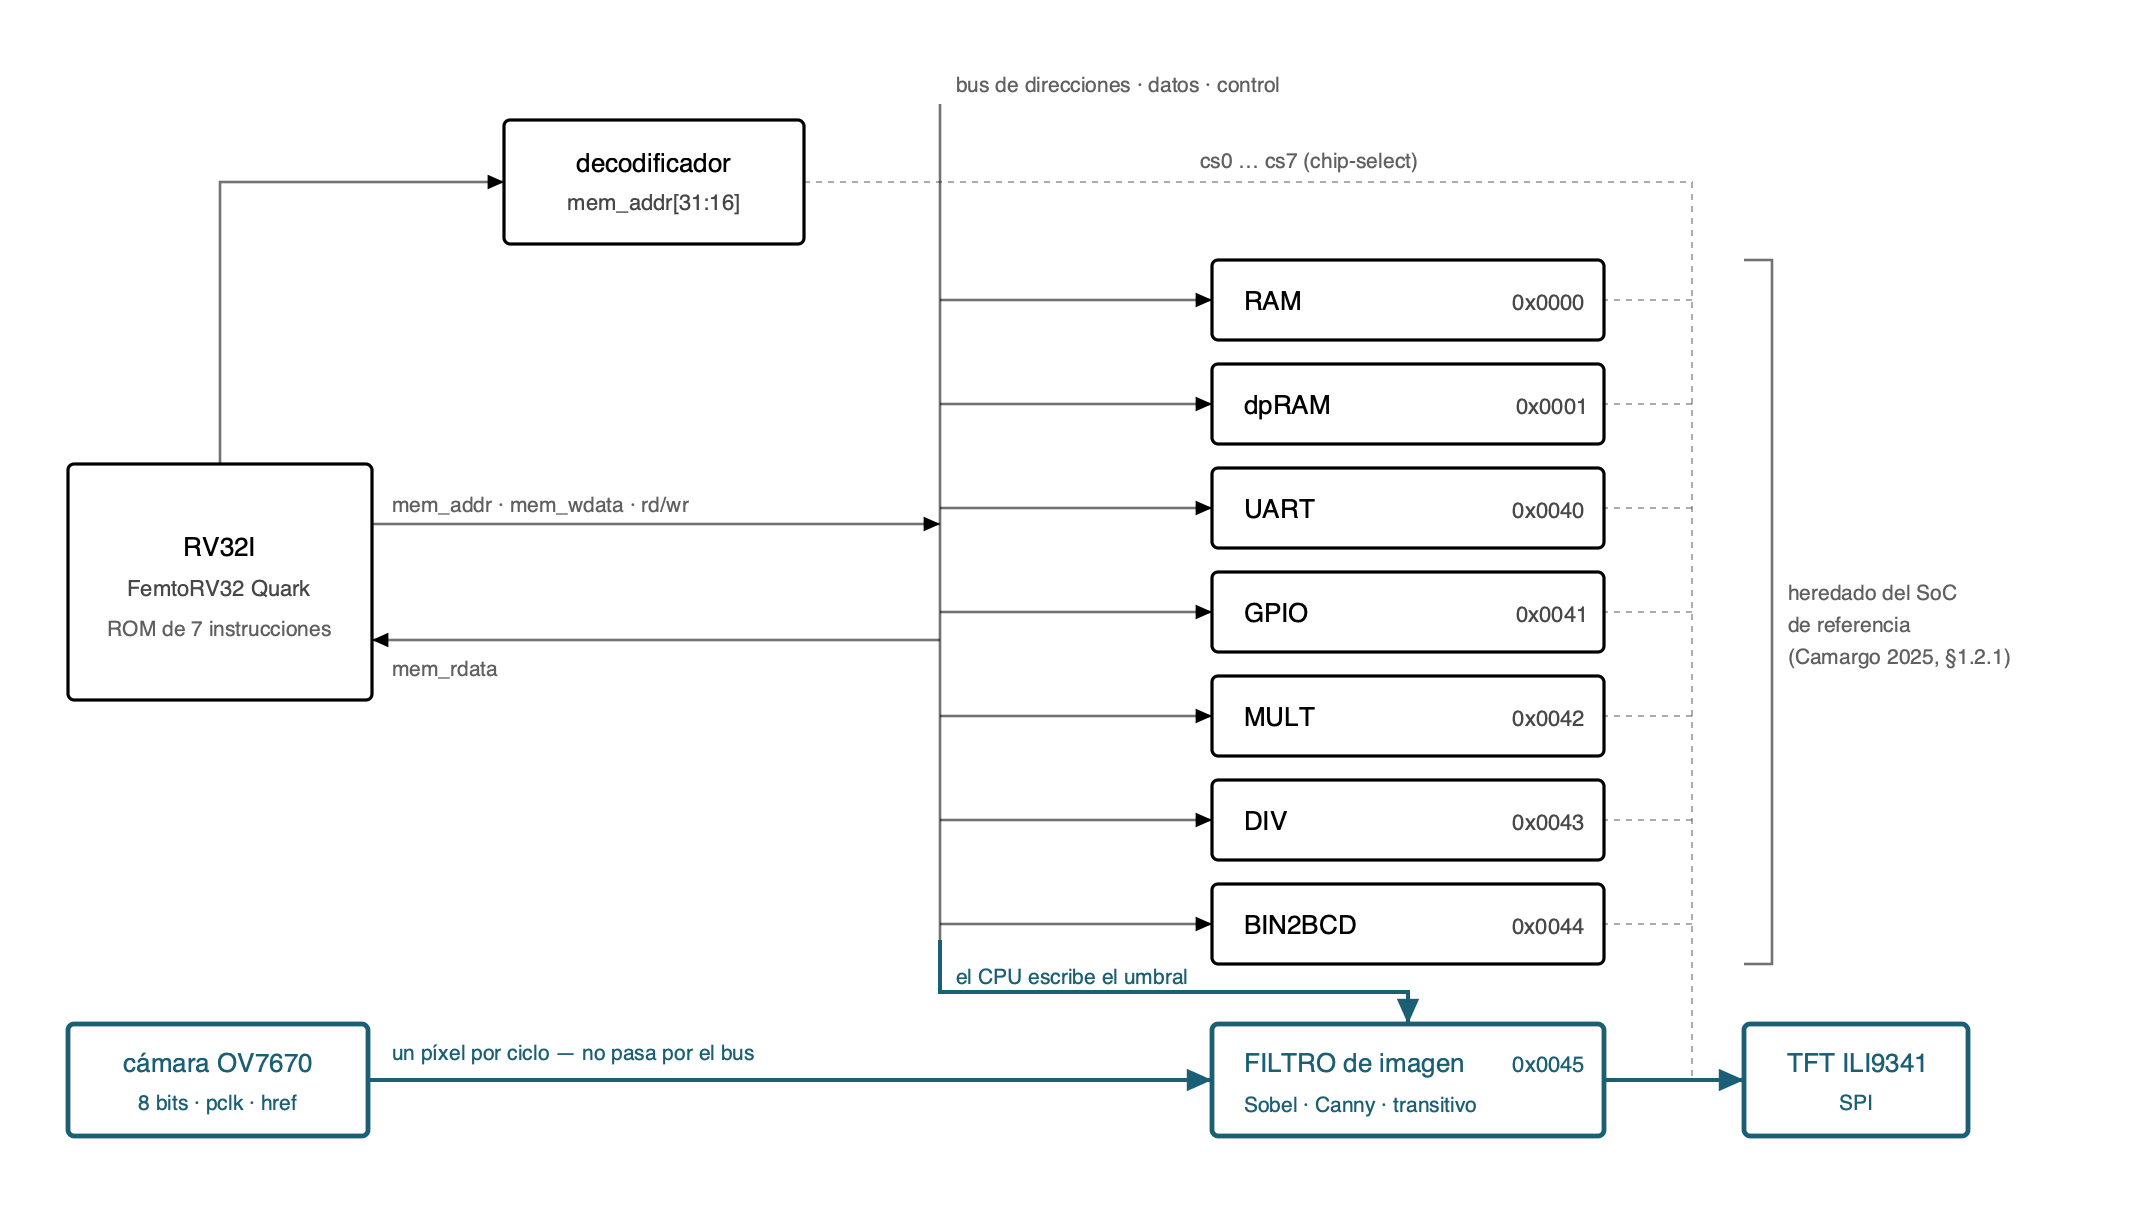
\includegraphics[keepaspectratio,alt={Figura 4.1. El sistema en silicio, en el lenguaje de bloques del SoC de referencia. Los siete periféricos en gris son los heredados; el que aparece destacado, en la base 0x0045, es la aportación de este trabajo. Obsérvese que el camino de datos de imagen no pasa por el bus: los píxeles entran de la cámara al filtro y salen de éste a la pantalla a un píxel por ciclo, y lo único que el procesador pone en el bus es el umbral.}]{figuras/fig_4_1_soc.png}}
\caption{\textbf{Figura 4.1.} El sistema en silicio, en el lenguaje de
bloques del SoC de referencia. Los siete periféricos en gris son los
heredados; el que aparece destacado, en la base \texttt{0x0045}, es la
aportación de este trabajo. Obsérvese que \textbf{el camino de datos de
imagen no pasa por el bus}: los píxeles entran de la cámara al filtro y
salen de éste a la pantalla a un píxel por ciclo, y lo único que el
procesador pone en el bus es el umbral.}
\end{figure}

La figura muestra por qué este periférico no se parece a los demás. Un
multiplicador o un divisor reciben sus operandos por el bus y devuelven
el resultado por el bus: el procesador los usa. El filtro, en cambio,
\textbf{tiene su propio camino de datos} ---de la cámara a la pantalla,
a un píxel por ciclo--- y del bus recibe únicamente un parámetro de
configuración. El procesador no lo usa: lo \textbf{ajusta}.

\begin{quote}
Esa distinción es la que el Capítulo 6 convierte en argumento. Un
periférico que procesa a través del bus está limitado por el ancho de
banda del bus; uno que procesa al margen de él, no. Es la razón de que
un sistema de visión en tiempo real pueda construirse sobre un
procesador de siete instrucciones.
\end{quote}

El firmware ocupa \textbf{siete instrucciones}: inicializa, escribe el
umbral y queda en un lazo. No es un programa modesto por limitación sino
por diseño --- el procesador existe para poder cambiar un parámetro en
tiempo de ejecución, no para procesar.

\subsection{La ROM sintetizada}\label{la-rom-sintetizada}

En una FPGA el contenido de la memoria de programa se carga con el
\emph{bitstream}. \textbf{En un ASIC no hay nada que lo cargue}: los
biestables arrancan en un estado indefinido. La memoria de programa debe
por tanto sintetizarse como lógica combinacional ---una tabla de
constantes--- y no como un arreglo inicializado.

Es el primero de los cuatro cambios obligatorios de la §4.8, y el que
más sorprende a quien llega desde FPGA, porque el código funciona
idénticamente en simulación en ambos casos.

\section{4.6 Memoria: la batalla de los
recursos}\label{memoria-la-batalla-de-los-recursos}

La iCE40UP5K ofrece tres clases de almacenamiento, y el diseño usa las
tres con criterios distintos:

\begin{longtable}[]{@{}
  >{\raggedright\arraybackslash}p{(\linewidth - 4\tabcolsep) * \real{0.3333}}
  >{\raggedright\arraybackslash}p{(\linewidth - 4\tabcolsep) * \real{0.3333}}
  >{\raggedright\arraybackslash}p{(\linewidth - 4\tabcolsep) * \real{0.3333}}@{}}
\toprule\noalign{}
\begin{minipage}[b]{\linewidth}\raggedright
Recurso
\end{minipage} & \begin{minipage}[b]{\linewidth}\raggedright
Cantidad
\end{minipage} & \begin{minipage}[b]{\linewidth}\raggedright
Uso en este trabajo
\end{minipage} \\
\midrule\noalign{}
\endhead
\bottomrule\noalign{}
\endlastfoot
Celdas lógicas & 5 280 & lógica y registros pequeños \\
Bloques de memoria (4 kbit) & 30 & \textbf{memorias de línea} de las
ventanas 3×3 \\
SPRAM (256 kbit) & 4 & \textbf{framebuffers} del filtro transitivo \\
\end{longtable}

La asignación no es libre: una memoria de línea cabe en un bloque de
memoria si el sintetizador la reconoce como tal, y no la reconoce si el
código la escribe de una forma que no encaja con el patrón esperado.
Varios de los problemas de recursos del desarrollo fueron de esa
naturaleza ---memorias que se convertían en biestables por un detalle de
escritura del RTL--- y no de tamaño real del diseño.

El caso más costoso fue un \textbf{ancho de puntero insuficiente}: un
contador de direcciones con un bit de menos del necesario direcciona la
mitad de la memoria y sobrescribe la otra, produciendo una imagen que se
ve plausible pero está mal. Como en el caso del byte de luminancia, el
error sobrevive a la inspección visual.

\begin{quote}
Este apartado es el origen del título del Capítulo 6. En la FPGA los dos
primeros recursos parecen gratuitos porque ya están en el sustrato; en
el ASIC ninguno lo es, y el mismo RTL que allí cabía holgadamente aquí
define el tamaño del dado.
\end{quote}

\section{4.7 Del RTL a la FPGA}\label{del-rtl-a-la-fpga}

El camino a la FPGA impuso sus propias decisiones.

\textbf{El intercambio entre celdas lógicas y bloques de memoria.}
Forzar más memorias de línea a bloques libera celdas pero consume
bloques, que son treinta. En varios puntos del desarrollo el diseño
estuvo limitado alternativamente por uno y por otro, y la solución
consistió en mover recursos entre ambos hasta encontrar una combinación
que cerrara.

\textbf{El bug del cerrojo.} Una asignación condicional incompleta
dentro de un bloque combinacional infiere un cerrojo en lugar de lógica.
El diseño sintetiza, ocupa recursos parecidos y funciona en simulación;
en la placa produce un comportamiento dependiente de la temporización.
La herramienta lo advierte, y la advertencia es fácil de ignorar entre
otras muchas.

\textbf{El bring-up incremental.} El sistema se puso en marcha por
etapas, cada una verificable por sí misma: parpadeo, reloj,
configuración SCCB, imagen en gris, memorias de línea, filtro, umbral,
motor, procesador. La razón es que \textbf{cada etapa es el banco de
pruebas de la siguiente}: cuando el filtro no produjo imagen, disponer
de la etapa anterior funcionando permitió decidir en un solo intento si
el problema estaba en el filtro o en la captura.

\section{4.8 Del RTL al ASIC: los cuatro cambios
obligatorios}\label{del-rtl-al-asic-los-cuatro-cambios-obligatorios}

El mismo Verilog no sirve para los dos destinos. Cuatro cosas hay que
cambiar, y ninguna de ellas produce un error de simulación ---por eso
son peligrosas.

\textbf{1. La memoria de programa debe sintetizarse.} Ya explicado en la
§4.5: en silicio no existe el \emph{bitstream} que la inicializa.

\textbf{2. Reset explícito en todos los registros de control.} En una
FPGA los biestables arrancan en el valor que el \emph{bitstream} les da;
en silicio arrancan en un estado indefinido. Toda máquina de estados
necesita una señal de reinicio explícita, y omitirla produce un circuito
que en simulación arranca correctamente y en la mesa no arranca nunca.

\textbf{3. Fuera el tri-estado interno.} El bus de datos de la cámara es
bidireccional y en FPGA se describe con alta impedancia dentro del
diseño. Un ASIC de celda estándar no dispone de eso: la señal debe
partirse en un dato y un habilitador ---\texttt{cam\_sda\_o} y
\texttt{cam\_sda\_oe}--- y el tri-estado real ocurre en el anillo de
pads.

\textbf{4. Fuera las primitivas del fabricante.} Los bloques específicos
de Lattice ---el controlador del LED RGB, entre otros--- no existen en
sky130. Se sustituyen por pines ordinarios o se eliminan.

\begin{quote}
Los cuatro cambios comparten una propiedad que conviene subrayar:
\textbf{ninguno produce un fallo visible en simulación RTL}. Un diseño
con \texttt{initial} heredado de FPGA simula perfectamente y sale de
fábrica mudo. Los dos únicos que se detectaron a tiempo durante este
trabajo aparecieron en \textbf{simulación de compuertas}, después de la
síntesis, y no antes.
\end{quote}

\chapter{5. Resultados}\label{resultados}

\section{5.1 Verificación funcional}\label{verificaciuxf3n-funcional}

\begin{quote}
\textbf{Estado:} borrador 1, escrito el 2026-09-16. Fuente: cuaderno 1,
Partes 29-35. Formato Markdown para convertir con \texttt{pandoc} a Word
o LaTeX según decida la guía de la Facultad.
\end{quote}

Antes de presentar área, frecuencia o consumo conviene establecer que
los circuitos \textbf{calculan lo que deben calcular}. Esta sección lo
hace, y distingue con cuidado dos preguntas que la literatura de
implementación mezcla con frecuencia: si el hardware coincide con su
modelo de referencia, y si el resultado es bueno. Aquí sólo se responde
la primera. La segunda pertenece a la §5.6.

\subsection{5.1.1 El criterio}\label{el-criterio}

Cada filtro se especificó primero como un programa en Python ---el
\textbf{modelo golden} descrito en la §3.2--- y sólo después se escribió
su descripción en Verilog. La verificación consiste en ejecutar ambos
sobre la misma entrada y comparar \textbf{píxel a píxel}, no en
inspeccionar visualmente la salida.

La distinción no es formal. Un mapa de bordes erróneo sigue pareciendo
un mapa de bordes, de modo que la inspección visual no distingue un
circuito correcto de uno que desplaza una fila, satura un byte o
invierte un signo. Sólo la comparación numérica lo hace.

Al comparar se admite un \textbf{desplazamiento constante} entre ambas
salidas ---la técnica de \emph{best-shift} de la §3.3--- porque la
implementación en hardware introduce una latencia de segmentación que el
modelo en software no tiene. Un desfase uniforme de \emph{k} píxeles no
es un error de cálculo sino una propiedad de la arquitectura segmentada,
y se descuenta explícitamente; cualquier diferencia que sobreviva a esa
corrección sí lo es.

\subsection{5.1.2 Resultado sobre los núcleos
aislados}\label{resultado-sobre-los-nuxfacleos-aislados}

Los tres núcleos son \textbf{idénticos bit a bit} a su modelo de
referencia. En el caso del Sobel sobre un cuadro de 60×80, la
comparación arroja \textbf{0 píxeles de diferencia sobre 4 800}, y el
resultado se sostiene para los tres filtros sobre las cinco imágenes de
prueba.

\begin{longtable}[]{@{}lrrr@{}}
\toprule\noalign{}
Núcleo & Imágenes & Píxeles comparados & Diferencias \\
\midrule\noalign{}
\endhead
\bottomrule\noalign{}
\endlastfoot
Sobel 3×3 & 5 / 5 & 4 800 por cuadro & \textbf{0} \\
Canny de un salto & 5 / 5 & 4 800 por cuadro & \textbf{0} \\
Canny transitivo & 5 / 5 & 4 800 por cuadro & \textbf{0} \\
\end{longtable}

Que la coincidencia sea exacta y no aproximada tiene una causa de
diseño: los tres filtros operan \textbf{sobre enteros y sin división}.
La magnitud del gradiente usa la norma L1,
\texttt{\textbar{}Gx\textbar{}+\textbar{}Gy\textbar{}}, en lugar de la
euclídea; los pesos del operador son potencias de dos, implementadas
como desplazamientos; y el umbral es una comparación. No hay ninguna
operación cuyo redondeo pueda diferir entre una biblioteca de punto
flotante y un circuito. \textbf{La igualdad bit a bit no es una
casualidad afortunada: es consecuencia de haber elegido una aritmética
que la permite.}

\subsection{5.1.3 Resultado sobre la cadena completa con
cámara}\label{resultado-sobre-la-cadena-completa-con-cuxe1mara}

La verificación anterior alimenta el circuito con una imagen almacenada.
La cadena real recibe en cambio un flujo de video de la cámara OV7670,
con sus bordes de línea, sus tiempos muertos y su sincronismo propio.
Medida sobre ese flujo, la concordancia entre el hardware y el modelo
es:

\begin{longtable}[]{@{}lr@{}}
\toprule\noalign{}
Cadena & Concordancia \\
\midrule\noalign{}
\endhead
\bottomrule\noalign{}
\endlastfoot
Sobel & 95 -- 100 \% \\
Canny de un salto & 88 -- 99 \% \\
Canny transitivo & 96 -- 100 \% \\
Promedio a través del SoC & \textbf{97,8 \%} \\
\end{longtable}

La degradación respecto del 100 \% de la §5.1.2 no proviene del filtro
sino del \textbf{acoplamiento con la cámara}: el muestreo del flujo, el
recorte de la ventana y el instante exacto en que empieza un cuadro
introducen diferencias de uno o dos píxeles en los bordes de la imagen.
El valor más bajo corresponde al Canny de un salto, que es también el
más sensible por construcción ---un píxel que cruza el umbral alto
propaga su decisión a sus vecinos, de modo que una diferencia aislada en
la entrada puede producir varias en la salida.

\begin{quote}
\textbf{Dos precisiones de terminología, porque el número se presta a
confusión.}

Primera: los porcentajes de esta tabla son \textbf{concordancia entre el
hardware y su propio modelo de referencia}, no exactitud del filtro.
Miden si el circuito hace lo que el programa hace, no si lo que el
programa hace es correcto o útil. Un filtro mal diseñado puede alcanzar
el 100 \% de concordancia con un modelo igualmente mal diseñado.

Segunda: la \textbf{densidad de bordes} ---la fracción de píxeles
marcados, en torno al 2 \% en las imágenes de prueba--- aparece en
varias figuras de este trabajo y \textbf{no es una medida de calidad}.
Es una propiedad de la escena y del punto de operación elegido, y su
valor «correcto» depende de para qué se vaya a usar el mapa de bordes.
La §5.6.4 muestra precisamente que mover ese punto de operación cambia
el resultado de clasificación más que cambiar de filtro.
\end{quote}

\section{5.2 Resultados en FPGA}\label{resultados-en-fpga}

\begin{quote}
\textbf{Estado:} borrador 2, 2026-09-21. Fuente: cuaderno 1, Partes
25-28 y 68-82, y los informes de \texttt{nextpnr-ice40} conservados de
las corridas del 30 de julio y del 3 de agosto de 2026.
\end{quote}

Los resultados de esta sección son de una clase distinta a los del resto
del capítulo: no provienen de un informe de herramienta sino de
\textbf{un circuito que funciona sobre una mesa}, con una cámara
apuntando a un objeto y una pantalla mostrando el resultado. Es la única
parte del trabajo donde el sistema completo existe físicamente, y por
eso condiciona lo que puede afirmarse de las demás.

\subsection{5.2.1 La plataforma}\label{la-plataforma}

La implementación física se realizó sobre una \textbf{iCE40UP5K} en
tarjeta iCESugar v1.5, con una cámara \textbf{OV7670} y una pantalla
\textbf{TFT ILI9341} por SPI. El flujo de síntesis e implementación es
enteramente abierto: \texttt{yosys} para síntesis,
\texttt{nextpnr-ice40} para emplazamiento y ruteo, \texttt{icepack} para
el \emph{bitstream}.

La elección del dispositivo no es incidental. La iCE40UP5K ofrece 5 280
celdas lógicas, 30 bloques de memoria de 4 kbit y \textbf{cuatro bloques
de SPRAM de 256 kbit} --- y son estos últimos los que hacen posible el
filtro transitivo, porque permiten alojar el cuadro completo sin
consumir lógica. Esa disponibilidad es exactamente lo que desaparece al
pasar a un ASIC sin macro de memoria, y es el origen del resultado de la
§5.4.3.

\subsection{5.2.2 Los tres filtros,
funcionando}\label{los-tres-filtros-funcionando}

\begin{longtable}[]{@{}
  >{\raggedright\arraybackslash}p{(\linewidth - 6\tabcolsep) * \real{0.2500}}
  >{\raggedright\arraybackslash}p{(\linewidth - 6\tabcolsep) * \real{0.2500}}
  >{\raggedright\arraybackslash}p{(\linewidth - 6\tabcolsep) * \real{0.2500}}
  >{\raggedright\arraybackslash}p{(\linewidth - 6\tabcolsep) * \real{0.2500}}@{}}
\toprule\noalign{}
\begin{minipage}[b]{\linewidth}\raggedright
Filtro
\end{minipage} & \begin{minipage}[b]{\linewidth}\raggedright
Arquitectura
\end{minipage} & \begin{minipage}[b]{\linewidth}\raggedright
Implementación física
\end{minipage} & \begin{minipage}[b]{\linewidth}\raggedright
Umbrales en la placa
\end{minipage} \\
\midrule\noalign{}
\endhead
\bottomrule\noalign{}
\endlastfoot
Sobel & flujo & hardware, con procesador FemtoRV32 & 90 \\
Canny de un salto & flujo & hardware, con procesador FemtoRV32 & 50 /
20 \\
Canny transitivo & \textbf{framebuffer} & hardware, motor en Verilog
\textbf{sin procesador} & 60 / 30 \\
\end{longtable}

Los tres funcionan sobre la placa con cámara y pantalla en vivo. El
transitivo produce contornos \textbf{conectados y completos} ---una
letra cerrada aparece cerrada--- frente a los bordes locales de los
otros dos, que es precisamente lo que su punto fijo debe conseguir.

\begin{figure}
\centering
\pandocbounded{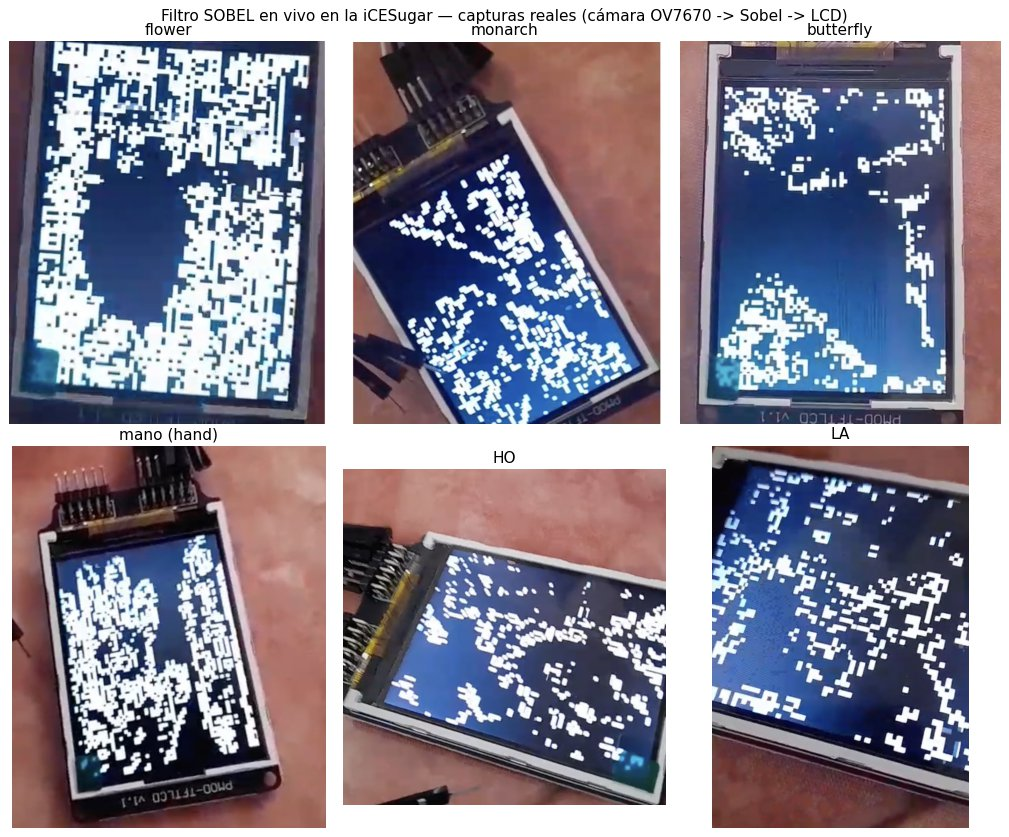
\includegraphics[keepaspectratio,alt={Figura 5.1. El filtro Sobel corriendo en vivo sobre la iCESugar, fotografiado directamente de la pantalla. Seis escenas distintas ---una flor, dos mariposas, una mano y dos letras--- recorren la cadena completa cámara → filtro → pantalla sin intervención de ningún computador. Son capturas del montaje físico, no reconstrucciones: la propia tarjeta y el cableado del módulo aparecen en el encuadre.}]{figuras/fig_5_1_sobel_en_vivo.jpg}}
\caption{\textbf{Figura 5.1.} El filtro Sobel corriendo en vivo sobre la
iCESugar, fotografiado directamente de la pantalla. Seis escenas
distintas ---una flor, dos mariposas, una mano y dos letras--- recorren
la cadena completa cámara → filtro → pantalla sin intervención de ningún
computador. Son capturas del montaje físico, no reconstrucciones: la
propia tarjeta y el cableado del módulo aparecen en el encuadre.}
\end{figure}

\subsection{5.2.3 Utilización del
dispositivo}\label{utilizaciuxf3n-del-dispositivo}

La tabla recoge el \textbf{Device utilisation} que informa
\texttt{nextpnr-ice40} tras el emplazamiento y ruteado
---\texttt{-\/-up5k\ -\/-package\ sg48}---, que es la medida
autoritativa: la que dice si el diseño entra en el dispositivo. Las
cinco filas de una misma columna proceden de \textbf{una sola corrida
con una sola versión de las herramientas}, para que sean comparables
entre sí.

\begin{longtable}[]{@{}
  >{\raggedright\arraybackslash}p{(\linewidth - 12\tabcolsep) * \real{0.1111}}
  >{\raggedleft\arraybackslash}p{(\linewidth - 12\tabcolsep) * \real{0.1481}}
  >{\raggedleft\arraybackslash}p{(\linewidth - 12\tabcolsep) * \real{0.1481}}
  >{\raggedleft\arraybackslash}p{(\linewidth - 12\tabcolsep) * \real{0.1481}}
  >{\raggedleft\arraybackslash}p{(\linewidth - 12\tabcolsep) * \real{0.1481}}
  >{\raggedleft\arraybackslash}p{(\linewidth - 12\tabcolsep) * \real{0.1481}}
  >{\raggedleft\arraybackslash}p{(\linewidth - 12\tabcolsep) * \real{0.1481}}@{}}
\toprule\noalign{}
\begin{minipage}[b]{\linewidth}\raggedright
Diseño
\end{minipage} & \begin{minipage}[b]{\linewidth}\raggedleft
LC / 5 280
\end{minipage} & \begin{minipage}[b]{\linewidth}\raggedleft
BRAM / 30
\end{minipage} & \begin{minipage}[b]{\linewidth}\raggedleft
SPRAM / 4
\end{minipage} & \begin{minipage}[b]{\linewidth}\raggedleft
E/S / 39
\end{minipage} & \begin{minipage}[b]{\linewidth}\raggedleft
\emph{f}máx sistema
\end{minipage} & \begin{minipage}[b]{\linewidth}\raggedleft
\emph{f}máx cámara
\end{minipage} \\
\midrule\noalign{}
\endhead
\bottomrule\noalign{}
\endlastfoot
Transitivo, motor dedicado \textbf{sin procesador} & 2 426 (45 \%) & 17
(56 \%) & \textbf{2 (50 \%)} & 18 (46 \%) & \textbf{28,7 MHz} ✓ & 20,6
MHz ✓ \\
SoC + Sobel & 4 848 (91 \%) & 20 (66 \%) & 0 & 18 (46 \%) & 9,5 MHz ✗ &
20,7 MHz ✓ \\
SoC + Canny de un salto & 5 234 (\textbf{99 \%}) & 24 (80 \%) & 0 & 18
(46 \%) & 9,5 MHz ✗ & 17,7 MHz ✓ \\
SoC + transitivo \textbf{por software} & 5 251 (\textbf{99 \%}) & 28 (93
\%) & 0 & 18 (46 \%) & 8,7 MHz ✗ & 20,5 MHz ✓ \\
SoC + transitivo \textbf{como periférico} & no emplaza (≈ 127 \%) & ---
& --- & --- & --- & --- \\
\end{longtable}

\begin{quote}
\textbf{Procedencia.} Las cuatro primeras filas se midieron de nuevo
para este documento. Tres de ellas ---las filas primera, tercera y
cuarta--- reprodujeron \textbf{exactamente}, celda por celda y bloque
por bloque, los informes conservados de las corridas originales de julio
y agosto de 2026. La del SoC + Sobel, cuyo informe de emplazamiento no
se había conservado, arrojó 4 848 celdas frente a las 4 878 anotadas
entonces en el cuaderno; la diferencia, de treinta celdas sobre cinco
mil, proviene de una versión distinta del sintetizador, que produce doce
tablas de consulta menos. La quinta fila no dispone de informe: el
emplazamiento no llegó a completarse, y el ≈ 127 \% es el valor
documentado en su momento.
\end{quote}

De la tabla se desprenden tres lecturas.

\textbf{La memoria grande sólo la usa un diseño.} Los cuatro bloques de
SPRAM ---256 kbit cada uno--- están sin tocar en todas las variantes de
flujo, y sólo el transitivo consume dos. Es coherente con su
arquitectura: es el único que necesita el cuadro entero a la vez. Los
filtros de flujo se las arreglan con dos filas de retardo, que caben en
los bloques de memoria pequeños.

\textbf{El límite de frecuencia lo pone el procesador, y no la
ocupación.} Los tres diseños que llevan el FemtoRV32 se agrupan entre
8,7 y 9,5 MHz mientras que el que no lo lleva alcanza 28,7 MHz:
\textbf{tres veces más rápido}. La tentación es atribuirlo a la
congestión ---los dos más lentos están al 99 \%---, pero la tabla lo
desmiente: el SoC del Sobel, \textbf{ocho puntos más vacío} que el del
Canny, cierra a la misma frecuencia, y de hecho una centésima por
debajo. La causa está en el informe de caminos críticos, que en los tres
SoC señala el mismo origen: \textbf{el registro de instrucción del
procesador}. El camino va de un flanco de subida a uno de bajada, de
modo que dispone de \textbf{medio período} en lugar de uno entero, y eso
divide por dos la frecuencia alcanzable. La síntesis lo confirma por
otra vía: los tres SoC contienen \textbf{2 048 biestables sensibles al
flanco de bajada} y el diseño sin procesador no contiene
\textbf{ninguno}. No es un problema de emplazamiento sino una propiedad
del procesador elegido, y es la razón de fondo de que las tres variantes
con CPU necesiten dividir el reloj.

\textbf{El sensor nunca fue el límite.} El dominio de la cámara cierra
con holgura en las cuatro filas medidas ---entre 17,7 y 20,7 MHz frente
a los 12 necesarios---, y es el del sistema el que falla. El cuello de
botella está del lado del procesamiento, no de la adquisición.

\begin{quote}
\textbf{Y una observación sobre el sustrato.} En los cuatro diseños el
retardo del camino crítico está dominado por el \textbf{ruteado}, que
aporta entre el 62 \% y el 72 \% del total; la lógica aporta el resto.
En una malla de interconexión fija como la de una FPGA esto es lo
esperable, y conviene tenerlo presente al leer la §5.4: en el ASIC,
donde el trazado se genera para el diseño concreto, ese reparto es otro.
\end{quote}

\subsection{5.2.4 El hallazgo de
co-diseño}\label{el-hallazgo-de-co-diseuxf1o}

El dato más importante de esta sección no es una cifra de utilización
sino una \textbf{decisión de arquitectura que la medida forzó}.

La intención inicial era que el procesador calculara la histéresis
transitiva por software, como hace en las versiones de los otros dos
filtros. Esa versión existe y funciona en simulación, con un 92,8 \% de
concordancia. Pero al intentar sintetizar el conjunto ---procesador,
memoria, framebuffers y motor--- la ocupación de celdas lógicas alcanzó
el \textbf{127 \%}: no cabía.

La respuesta fue mover el motor de histéresis de software a hardware,
como camino de datos en Verilog sin intervención del procesador. Así
implementado, la síntesis reporta \textbf{1 728 tablas de consulta} y el
emplazamiento \textbf{2 426 celdas lógicas, el 45 \% del dispositivo},
cerrando el temporizado a \textbf{28,7 MHz} con holgura.

\begin{quote}
Las dos cifras anteriores no son la misma medida, y conviene no
confundirlas: la celda lógica de la iCE40 empaqueta una tabla de
consulta \textbf{y} un biestable, de modo que un diseño con muchos
biestables sueltos ocupa más celdas que tablas tiene. Dividir el
recuento de tablas entre las 5 280 celdas del dispositivo da un 33 \%
que \textbf{subestima la ocupación real en doce puntos}. La cifra válida
es la del emplazamiento, no la de la síntesis; esta sección usa sólo la
primera.
\end{quote}

\begin{quote}
\textbf{Por qué esto es co-diseño y no una optimización.} No se trata de
que el hardware sea más rápido que el software, que es lo esperable. Se
trata de que \textbf{la restricción de recursos cambió el reparto de
responsabilidades entre las dos mitades del sistema}: la misma función,
expresada como programa, no cabía; expresada como circuito, ocupa un
tercio del dispositivo. La frontera entre lo que ejecuta el procesador y
lo que ejecuta la lógica dedicada no la fijó una preferencia de diseño
sino una medición.
\end{quote}

Este resultado reaparece transformado en la §5.4.2: en el ASIC, donde el
área no está acotada por un dispositivo fijo, el procesador vuelve a ser
viable junto al transitivo y cuesta unas nueve mil celdas. La misma
pregunta tiene respuestas opuestas en los dos sustratos.

\subsection{5.2.5 Umbrales de laboratorio y umbrales de
cámara}\label{umbrales-de-laboratorio-y-umbrales-de-cuxe1mara}

Las tres filas de la tabla anterior muestran umbrales distintos de los
que se usan en simulación. El transitivo, por ejemplo, pasó de 110/70 en
el banco de pruebas a \textbf{60/30 en la placa}.

El ajuste no es arbitrario ni es un defecto: una imagen almacenada y un
flujo de cámara tienen histogramas distintos, y el punto de operación
que extrae la estructura de una no es el que la extrae de la otra. La
§5.6.4 mide exactamente cuánto importa esa elección, y muestra que
\textbf{mover el umbral dentro de un filtro cambia el resultado de
clasificación más que cambiar de filtro}.

\begin{center}\rule{0.5\linewidth}{0.5pt}\end{center}

\begin{quote}
\textbf{Sobre la reproducibilidad de estas cifras.} Las cuatro filas
medidas se rehicieron el 21 de septiembre de 2026 con el guion
\texttt{medir\_utilizacion\_vm.sh}, que aplica a cada diseño las mismas
órdenes de lectura de fuentes que su guion de construcción original.
Tres de las cuatro reprodujeron el informe conservado sin desviarse en
una sola celda ni en un solo bloque de memoria, pese a mediar casi dos
meses entre una corrida y otra. La cuarta se desvió en treinta celdas
sobre cinco mil, y la causa está identificada: una versión distinta del
sintetizador. \textbf{El flujo es determinista a herramientas iguales},
que es lo que permite presentar estas cifras como medidas y no como
estimaciones.
\end{quote}

\section{5.3 Resultados en ASIC: los
bloques}\label{resultados-en-asic-los-bloques}

\begin{quote}
\textbf{Estado:} borrador 1, escrito el 2026-09-16. Fuente: cuaderno 1,
Partes 86-131, y el archivo de planos \texttt{ASIC\_planos/}.
\textbf{Recuento homogeneizado el 21 de septiembre de 2026.} Toda la
columna «celdas» de esta tabla son \textbf{celdas lógicas tras
emplazamiento y ruteado}, recontadas con un mismo criterio desde los
netlists archivados. Véase la §5.3.3 para cruzarlas con las de la §5.4.
\end{quote}

Esta sección presenta los circuitos que implementan \textbf{una función
cada uno}: los tres filtros por separado, los mismos con procesador, dos
bloques de interfaz y dos sistemas de visión. Son el vocabulario con el
que se construyen los sistemas de la §5.4, y su valor está en que
permiten atribuir el costo de cada pieza por separado.

Todos se llevaron a GDSII con \textbf{OpenLane} sobre el PDK abierto
\textbf{sky130A}, biblioteca \texttt{sky130\_fd\_sc\_hd}.

\subsection{5.3.1 La tabla}\label{la-tabla}

\begin{longtable}[]{@{}
  >{\raggedright\arraybackslash}p{(\linewidth - 8\tabcolsep) * \real{0.1765}}
  >{\raggedright\arraybackslash}p{(\linewidth - 8\tabcolsep) * \real{0.1765}}
  >{\raggedleft\arraybackslash}p{(\linewidth - 8\tabcolsep) * \real{0.2353}}
  >{\raggedleft\arraybackslash}p{(\linewidth - 8\tabcolsep) * \real{0.2353}}
  >{\centering\arraybackslash}p{(\linewidth - 8\tabcolsep) * \real{0.1765}}@{}}
\toprule\noalign{}
\begin{minipage}[b]{\linewidth}\raggedright
Circuito
\end{minipage} & \begin{minipage}[b]{\linewidth}\raggedright
Función
\end{minipage} & \begin{minipage}[b]{\linewidth}\raggedleft
Área del die
\end{minipage} & \begin{minipage}[b]{\linewidth}\raggedleft
Celdas
\end{minipage} & \begin{minipage}[b]{\linewidth}\centering
Signoff
\end{minipage} \\
\midrule\noalign{}
\endhead
\bottomrule\noalign{}
\endlastfoot
\texttt{sobel} & filtro Sobel 3×3 & 0,167 mm² & 5 823 & DRC/LVS/XOR =
0 \\
\texttt{canny1} & Canny de un salto, en flujo & 0,360 mm² & 12 993 &
DRC/LVS/XOR = 0 \\
\texttt{transitivo} & Canny con histéresis transitiva & 3,13 mm² & 65
659 & DRC/LVS/XOR = 0 \\
\texttt{soc\_sobel} & FemtoRV32 + Sobel & 0,37 mm² & 12 043 &
DRC/LVS/XOR = 0 \\
\texttt{soc\_canny1} & FemtoRV32 + Canny de un salto & 0,67 mm² & 22 054
& DRC/LVS/XOR = 0 \\
\texttt{soc\_trans} & FemtoRV32 + transitivo & 3,42 mm² & 72 337 &
DRC/LVS/XOR = 0 \\
\texttt{cam\_frontend} & front-end de cámara OV7670 & 0,0177 mm² & 562 &
DRC/LVS/XOR = 0 \\
\texttt{lcd\_ili9341} & driver de pantalla TFT por SPI & 0,0174 mm² &
553 & DRC/LVS/XOR = 0 \\
\texttt{vision\_top} & cámara + Sobel + framebuffer + pantalla & 1,75
mm² & 35 653 & DRC/LVS/XOR = 0 \\
\texttt{vision\_canny} & cámara + Canny + framebuffer + pantalla & 2,04
mm² & 41 925 & DRC/LVS/XOR = 0 \\
\end{longtable}

\textbf{Diez circuitos, diez veces DRC, LVS y XOR en cero.}

\subsection{5.3.2 Lo que la tabla muestra de un
vistazo}\label{lo-que-la-tabla-muestra-de-un-vistazo}

\textbf{El filtro transitivo cuesta casi veinte veces más área que el
Sobel} ---3,13 mm² contra 0,167, y once veces más celdas--- pese a
ejecutar aritmética comparable. La razón, ya anticipada, es el cuadro
completo residente: en la FPGA ese cuadro vivía en SPRAM y no consumía
lógica; aquí es un banco de biestables.

\textbf{Los dos bloques de interfaz son casi gratis.} El front-end de
cámara y el driver de pantalla ocupan menos de dieciocho milésimas de
milímetro cuadrado cada uno, alrededor de 560 celdas. Conviene tenerlo
medido porque desmonta una intuición común: el costo de un sistema de
visión embebido no está en hablar con los periféricos, está en lo que se
hace con los datos entre medias.

\begin{figure}
\centering
\pandocbounded{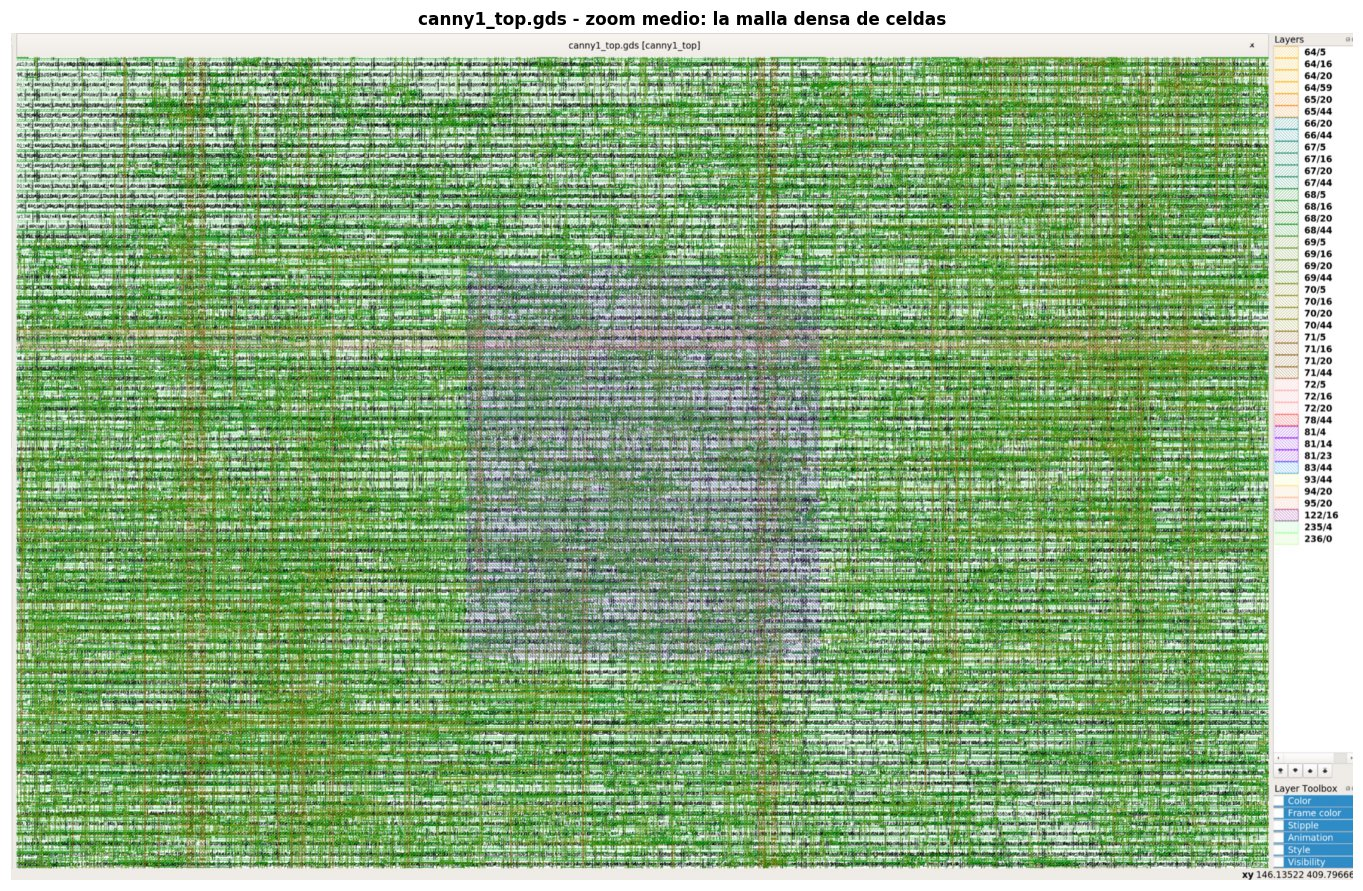
\includegraphics[keepaspectratio,alt={Figura 5.2. Acercamiento al GDSII del canny1 en KLayout. Lo que se ve no es un esquema sino el plano que iría a fábrica: filas de celdas estándar y, sobre ellas, las capas de metal que las conectan. La mancha más clara del centro es una región de menor densidad de ruteo. Las 12 993 celdas de la tabla anterior son, literalmente, estas.}]{figuras/fig_5_2_malla_canny1.jpg}}
\caption{\textbf{Figura 5.2.} Acercamiento al GDSII del \texttt{canny1}
en KLayout. Lo que se ve no es un esquema sino el plano que iría a
fábrica: filas de celdas estándar y, sobre ellas, las capas de metal que
las conectan. La mancha más clara del centro es una región de menor
densidad de ruteo. Las 12 993 celdas de la tabla anterior son,
literalmente, estas.}
\end{figure}

\textbf{Y el Sobel en silicio es mucho más rápido de lo que la FPGA
permitía.} Su camino crítico quedó en \textbf{7,69 ns} frente a un
objetivo de 20 ns, es decir que soportaría unos 130 MHz, mientras que en
la iCE40 cerraba entre 9 y 28 MHz. En silicio la lógica es rápida;
\textbf{lo caro es el área}, y ése es el eje sobre el que gira todo este
capítulo.

\subsection{5.3.3 El recuento de celdas, y cómo cruzar las dos
tablas}\label{el-recuento-de-celdas-y-cuxf3mo-cruzar-las-dos-tablas}

Esta advertencia no es un tecnicismo: afecta a cualquier comparación que
un lector intente hacer entre esta tabla y la de la §5.4.

Un circuito se puede contar en dos momentos del flujo, y las dos cifras
son legítimas:

\begin{longtable}[]{@{}
  >{\raggedright\arraybackslash}p{(\linewidth - 4\tabcolsep) * \real{0.3333}}
  >{\raggedright\arraybackslash}p{(\linewidth - 4\tabcolsep) * \real{0.3333}}
  >{\raggedright\arraybackslash}p{(\linewidth - 4\tabcolsep) * \real{0.3333}}@{}}
\toprule\noalign{}
\begin{minipage}[b]{\linewidth}\raggedright
Definición
\end{minipage} & \begin{minipage}[b]{\linewidth}\raggedright
Qué cuenta
\end{minipage} & \begin{minipage}[b]{\linewidth}\raggedright
Dónde se usa
\end{minipage} \\
\midrule\noalign{}
\endhead
\bottomrule\noalign{}
\endlastfoot
celdas de \textbf{síntesis} & el resultado de traducir el RTL a
compuertas & la tabla de la §5.4 \\
celdas \textbf{emplazadas} & lo que queda tras emplazar y rutear, con
los amortiguadores que el flujo inserta para el árbol de reloj y la
reparación de tiempos & \textbf{esta} tabla y la §5.6 \\
\end{longtable}

Durante la redacción, la columna «celdas» de este capítulo
\textbf{mezclaba las dos}, porque las fichas del cuaderno habían
registrado en cada momento el campo que la herramienta ofrecía.
\textbf{Se rehízo el recuento}: se contaron las instancias de celda
estándar directamente sobre el \textbf{netlist posterior al ruteado} de
cada circuito archivado, descartando las celdas sin función lógica
---relleno, contactos de pozo, desacoplo y diodos de antena---, con un
único criterio para los dieciséis.

El procedimiento se validó antes de aplicarlo: de los dieciséis
circuitos, \textbf{ocho reprodujeron exactamente la cifra que ya
constaba}, hasta la unidad ---los dos bloques de interfaz, los dos SoC,
los dos sistemas de visión y los dos circuitos en IHP---, que son
precisamente aquellos cuya ficha ya provenía del emplazamiento. Los ocho
restantes cambiaron, y ése era el objetivo.

\subsubsection{El factor de conversión,
medido}\label{el-factor-de-conversiuxf3n-medido}

Como en nueve circuitos se conservan las dos cifras, el paso de una a
otra no hay que estimarlo:

\begin{longtable}[]{@{}ll@{}}
\toprule\noalign{}
\endhead
\bottomrule\noalign{}
\endlastfoot
Casos medidos & 9 \\
Factor medio & \textbf{×1,21} \\
Mediana & ×1,20 \\
Rango & ×1,16 a ×1,26 \\
Desviación típica & 0,04 \\
\end{longtable}

\textbf{El emplazamiento agrega entre un 16 \% y un 26 \% de celdas},
con una dispersión estrecha. De modo que una cifra de la §5.4 se lleva a
la escala de ésta multiplicándola por 1,21, y el error de esa conversión
es de unos pocos puntos porcentuales --- no del 20 \% que separaba las
tablas antes de homogeneizarlas.

\begin{quote}
\textbf{Por qué no se convirtió también la §5.4.} Dos de sus seis
circuitos se archivaron sin netlist, de modo que convertir la tabla
habría exigido estimar dos de las seis filas. Se prefirió dejar cada
tabla \textbf{internamente homogénea} ---la §5.4 entera en celdas de
síntesis, ésta entera en celdas emplazadas--- y publicar el factor que
las relaciona, antes que producir una tabla mixta con dos filas
estimadas. Las comparaciones dentro de cada tabla son exactas; las que
cruzan de una a otra pasan por el factor.
\end{quote}

\section{5.4 Resultados en ASIC: la cadena de visión
completa}\label{resultados-en-asic-la-cadena-de-visiuxf3n-completa}

\begin{quote}
\textbf{Estado:} borrador 1, escrito el 2026-09-16. Fuente: cuaderno 1,
Partes 157-165, y la tabla maestra
\texttt{asic/tabla\_maestra/tabla\_6\_chips.py}, que la genera desde los
\texttt{metrics.csv} del flujo.
\end{quote}

La §5.3 presentó bloques: filtros solos, un front-end de cámara, un
driver de pantalla. Ésta presenta \textbf{sistemas}: seis circuitos que
llevan la cadena entera ---captura, filtrado, almacenamiento y
visualización--- en un solo dado. Los seis están organizados como una
matriz de dos variables, el \textbf{filtro} y la \textbf{presencia de
procesador}, de modo que cada comparación entre dos de ellos aísla una
sola causa.

\subsection{5.4.1 La tabla maestra}\label{la-tabla-maestra}

\begin{longtable}[]{@{}
  >{\raggedright\arraybackslash}p{(\linewidth - 20\tabcolsep) * \real{0.0811}}
  >{\raggedright\arraybackslash}p{(\linewidth - 20\tabcolsep) * \real{0.0811}}
  >{\raggedright\arraybackslash}p{(\linewidth - 20\tabcolsep) * \real{0.0811}}
  >{\centering\arraybackslash}p{(\linewidth - 20\tabcolsep) * \real{0.0811}}
  >{\raggedleft\arraybackslash}p{(\linewidth - 20\tabcolsep) * \real{0.1081}}
  >{\raggedleft\arraybackslash}p{(\linewidth - 20\tabcolsep) * \real{0.1081}}
  >{\raggedleft\arraybackslash}p{(\linewidth - 20\tabcolsep) * \real{0.1081}}
  >{\raggedleft\arraybackslash}p{(\linewidth - 20\tabcolsep) * \real{0.1081}}
  >{\centering\arraybackslash}p{(\linewidth - 20\tabcolsep) * \real{0.0811}}
  >{\centering\arraybackslash}p{(\linewidth - 20\tabcolsep) * \real{0.0811}}
  >{\centering\arraybackslash}p{(\linewidth - 20\tabcolsep) * \real{0.0811}}@{}}
\toprule\noalign{}
\begin{minipage}[b]{\linewidth}\raggedright
\#
\end{minipage} & \begin{minipage}[b]{\linewidth}\raggedright
Chip
\end{minipage} & \begin{minipage}[b]{\linewidth}\raggedright
Filtro
\end{minipage} & \begin{minipage}[b]{\linewidth}\centering
CPU
\end{minipage} & \begin{minipage}[b]{\linewidth}\raggedleft
Área (mm²)
\end{minipage} & \begin{minipage}[b]{\linewidth}\raggedleft
Celdas
\end{minipage} & \begin{minipage}[b]{\linewidth}\raggedleft
Reloj de firma
\end{minipage} & \begin{minipage}[b]{\linewidth}\raggedleft
Setup c/parásitos
\end{minipage} & \begin{minipage}[b]{\linewidth}\centering
DRC
\end{minipage} & \begin{minipage}[b]{\linewidth}\centering
LVS
\end{minipage} & \begin{minipage}[b]{\linewidth}\centering
XOR
\end{minipage} \\
\midrule\noalign{}
\endhead
\bottomrule\noalign{}
\endlastfoot
\#1 & \texttt{sobel\_completo} ᵃ & Sobel & --- & 2,45 & 36 730 & 20 ns
(50,0 MHz) & sin dato ᵇ & 0 & 0 & 0 \\
\#2 & \texttt{canny1\_completo} ᵃ & Canny1 & --- & 2,90 & 42 581 & 20 ns
(50,0 MHz) & sin dato ᵇ & 0 & 0 & 0 \\
\#3 & \texttt{trans\_completo} & Transitivo & --- & 9,61 & 137 092 & 20
ns (50,0 MHz) & \textbf{−19,35 ns} & 0 & 0 & 0 \\
\#4 & \texttt{soc\_sobel\_completo} & Sobel & ✓ & 3,03 & 46 019 & 32 ns
(31,2 MHz) & \textbf{+0,00 ns} & 0 & 0 & 0 \\
\#5 & \texttt{soc\_canny1\_completo} & Canny1 & ✓ & 3,44 & 51 037 & 36
ns (27,8 MHz) & \textbf{+0,00 ns} & 0 & 0 & 0 \\
\#6 & \texttt{soc\_trans\_completo} & Transitivo & ✓ & 10,19 & 146 216 &
36 ns (27,8 MHz) & \textbf{−18,23 ns} & 0 & 0 & 0 \\
\end{longtable}

ᵃ Estos dos se archivaron sin el directorio de reportes; sus cifras
provienen de la ficha del cuaderno y no de un \texttt{metrics.csv} del
flujo. Se marcan porque en una tabla de resultados debe poder decirse de
dónde sale cada número.

ᵇ Su ficha registra el \textbf{WNS nominal} ---0,00 ns, sin
violaciones--- pero no quedó registrado el setup ya con parásitos
extraídos, que es justamente la columna que hunde a los dos transitivos.
Se deja en blanco antes que suponer que cierran.

\textbf{Los seis llegaron a GDSII con DRC, LVS y XOR en cero.} Cuatro
cierran temporizado o carecen del dato para afirmar lo contrario; los
dos transitivos no cierran, y conviene decirlo con el número: el \#3
pediría 39,4 ns ---25,4 MHz--- y el \#6, 54,2 ns, es decir 18,4 MHz en
lugar de los 27,8 solicitados.

\begin{quote}
\textbf{Sobre el recuento de celdas, y es importante al leer junto a la
§5.3.} Las cifras de esta tabla son \textbf{celdas de síntesis}; las de
la §5.3 y la §5.6 son \textbf{celdas emplazadas}. Cada tabla es
internamente homogénea, y el paso de una escala a otra \textbf{está
medido sobre nueve circuitos que conservan las dos cifras}: el
emplazamiento agrega entre un 16 \% y un 26 \%, con un factor medio de
\textbf{×1,21} y una desviación típica de 0,04. Para comparar una cifra
de aquí con una de allá, multiplíquese por 1,21; el detalle del
procedimiento está en la §5.3.3.

Dos de los seis circuitos de esta tabla se archivaron sin
\emph{netlist}, razón por la cual no se convirtió la tabla entera: se
prefirió una tabla homogénea en su propia escala antes que una tabla
mixta con dos filas estimadas.
\end{quote}

\begin{figure}
\centering
\pandocbounded{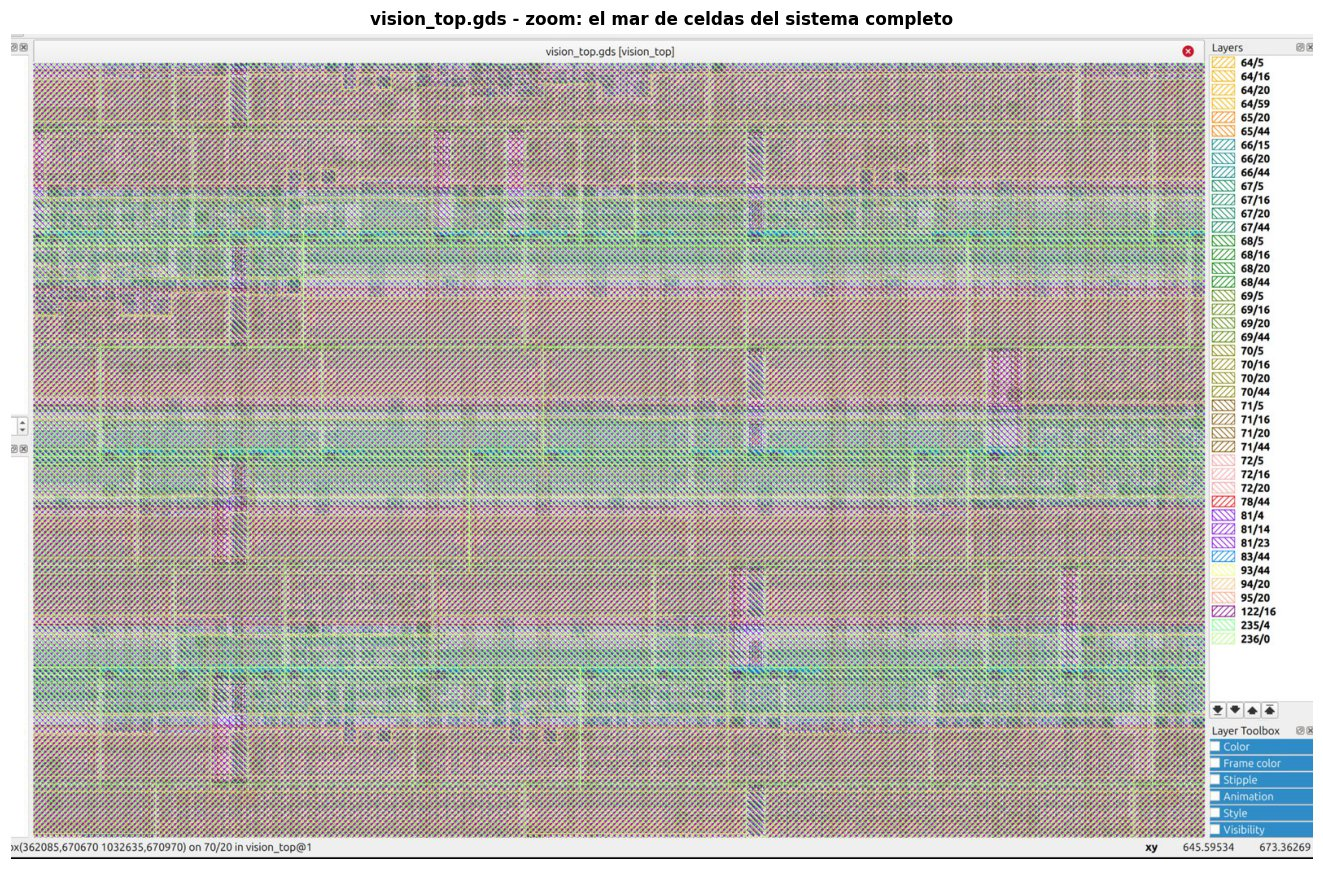
\includegraphics[keepaspectratio,alt={Figura 5.3. El mismo tipo de acercamiento, ahora sobre el sistema de visión completo. La diferencia con la figura anterior no está en la textura sino en la escala: aquí caben cámara, filtro, memoria de cuadro y controlador de pantalla en el mismo dado. Es la forma que toma en silicio la frase «el filtro es una pieza y no el circuito».}]{figuras/fig_5_3_mar_de_celdas_vision.jpg}}
\caption{\textbf{Figura 5.3.} El mismo tipo de acercamiento, ahora sobre
el sistema de visión completo. La diferencia con la figura anterior no
está en la textura sino en la escala: aquí caben cámara, filtro, memoria
de cuadro y controlador de pantalla en el mismo dado. Es la forma que
toma en silicio la frase «el filtro es una pieza y no el circuito».}
\end{figure}

\subsection{5.4.2 El procesador cuesta lo mismo, sea cual sea el
filtro}\label{el-procesador-cuesta-lo-mismo-sea-cual-sea-el-filtro}

Restando cada chip de su gemelo con procesador se obtiene el costo del
FemtoRV32, su memoria de programa y su periférico:

\begin{longtable}[]{@{}lrrrr@{}}
\toprule\noalign{}
Filtro & sin CPU & con CPU & Δ celdas & Δ relativo \\
\midrule\noalign{}
\endhead
\bottomrule\noalign{}
\endlastfoot
Sobel & 36 730 & 46 019 & \textbf{+9 289} & +25,3 \% \\
Canny de un salto & 42 581 & 51 037 & \textbf{+8 456} & +19,9 \% \\
Canny transitivo & 137 092 & 146 216 & \textbf{+9 124} & +6,7 \% \\
\end{longtable}

El incremento absoluto es \textbf{prácticamente constante}: alrededor de
nueve mil celdas, con una dispersión inferior al 5 \% entre el caso más
barato y el más caro. Es un resultado esperable ---el procesador no sabe
qué filtro tiene al lado--- pero conviene tenerlo medido, porque
convierte al procesador en un \textbf{costo fijo y presupuestable}
frente a un datapath cuyo costo varía en un factor de cuatro.

La columna relativa dice lo contrario que la absoluta, y las dos son
ciertas: el mismo procesador representa una cuarta parte del chip más
pequeño y apenas una quinceava parte del más grande. Cuál de las dos
lecturas importa depende de la pregunta. Para decidir si añadir un
procesador a un diseño dado, manda la absoluta.

\subsection{5.4.3 Lo que de verdad cuesta caro no es el cerebro: es la
memoria}\label{lo-que-de-verdad-cuesta-caro-no-es-el-cerebro-es-la-memoria}

El mismo ejercicio, hecho ahora sobre el eje del filtro en lugar del
procesador, produce el resultado central de este capítulo:

\begin{longtable}[]{@{}
  >{\raggedright\arraybackslash}p{(\linewidth - 6\tabcolsep) * \real{0.2143}}
  >{\raggedright\arraybackslash}p{(\linewidth - 6\tabcolsep) * \real{0.2143}}
  >{\raggedleft\arraybackslash}p{(\linewidth - 6\tabcolsep) * \real{0.2857}}
  >{\raggedleft\arraybackslash}p{(\linewidth - 6\tabcolsep) * \real{0.2857}}@{}}
\toprule\noalign{}
\begin{minipage}[b]{\linewidth}\raggedright
Alcance del patrón
\end{minipage} & \begin{minipage}[b]{\linewidth}\raggedright
Filtro
\end{minipage} & \begin{minipage}[b]{\linewidth}\raggedleft
Celdas (sin CPU)
\end{minipage} & \begin{minipage}[b]{\linewidth}\raggedleft
Δ respecto al anterior
\end{minipage} \\
\midrule\noalign{}
\endhead
\bottomrule\noalign{}
\endlastfoot
local, ventana 3×3 & Sobel & 36 730 & --- \\
local más un salto & Canny de un salto & 42 581 & +5 851 \\
\textbf{global, cuadro completo} & Canny transitivo & \textbf{137 092} &
\textbf{+94 511} \\
\end{longtable}

Pasar de mirar una ventana de 3×3 a mirar un salto más cuesta menos de
seis mil celdas. Pasar de ahí a \textbf{mirar el cuadro entero} cuesta
noventa y cuatro mil quinientas once.

La comparación directa es la que conviene enunciar: \textbf{un
procesador RISC-V completo, con su memoria y su periférico, pesa
aproximadamente la décima parte de lo que pesa cambiar el alcance del
patrón de local a global.} Nueve mil celdas contra noventa y cuatro mil
quinientas.

Y la razón no está en la aritmética. Los tres filtros ejecutan
esencialmente las mismas operaciones sobre cada píxel; lo que cambia es
\textbf{cuánto estado hay que sostener simultáneamente}. El Sobel y el
Canny de un salto procesan en flujo y necesitan unas pocas líneas de la
imagen ---los \emph{line-buffers} de la §4.6---, mientras que la
histéresis transitiva necesita el cuadro completo residente y accesible
en cualquier orden, porque su punto fijo puede propagar una decisión
desde cualquier píxel hacia cualquier otro. En una FPGA ese cuadro es un
bloque de memoria que ya está en el sustrato; en un ASIC sin macro de
memoria es un banco de biestables, y se paga en área, en potencia y en
frecuencia.

\begin{quote}
Éste es, en una sola cifra, el argumento que el Capítulo 6 desarrolla:
\textbf{lo que decide si un algoritmo cabe en silicio no es su
complejidad aritmética sino su huella de memoria.} Los dos transitivos
son además los dos únicos chips de la tabla que no cierran temporizado,
lo que muestra que el precio de esa memoria no se cobra sólo en
milímetros cuadrados.
\end{quote}

\subsection{5.4.4 Balance}\label{balance}

Seis circuitos, 459 675 celdas en total, \textbf{seis de seis con DRC =
LVS = XOR = 0}. Dos cierran temporizado con parásitos extraídos, dos
carecen de ese dato por haberse archivado sin reportes, y dos no cierran
y se documentan con la frecuencia que sí soportarían.

Ninguno ha sido fabricado. La §5.6.1 describe la vía por la que podrían
serlo.

\section{5.5 Rendimiento: caudal y
latencia}\label{rendimiento-caudal-y-latencia}

\begin{quote}
\textbf{Estado:} borrador 2, 2026-09-21. Fuente: cuaderno 1, Partes
154-156, y la corrida de \texttt{tb\_latencia\_final.v} del 21 de
septiembre. Todas las latencias de esta sección están \textbf{medidas en
simulación}, no estimadas --- incluida la del Canny, que hasta esta
versión provenía de una fórmula y resultó estar sobrestimada en un 20
\%.
\end{quote}

Las secciones anteriores midieron el costo de cada circuito. Ésta mide
su velocidad, y lo hace separando dos magnitudes que la palabra «rápido»
confunde: el \textbf{caudal}, o cuántos píxeles salen por segundo, y la
\textbf{latencia}, o cuánto tarda un píxel concreto desde que entra
hasta que sale.

La distinción importa porque las dos arquitecturas de este trabajo se
sitúan en extremos opuestos. Un cauce segmentado puede tener latencia
alta y caudal altísimo, porque los resultados salen uno tras otro una
vez lleno; y un motor iterativo puede terminar un cuadro entero de una
vez pero tardar milisegundos en hacerlo.

\subsection{5.5.1 Las dos arquitecturas}\label{las-dos-arquitecturas}

\begin{longtable}[]{@{}
  >{\raggedright\arraybackslash}p{(\linewidth - 4\tabcolsep) * \real{0.3333}}
  >{\raggedright\arraybackslash}p{(\linewidth - 4\tabcolsep) * \real{0.3333}}
  >{\raggedright\arraybackslash}p{(\linewidth - 4\tabcolsep) * \real{0.3333}}@{}}
\toprule\noalign{}
\begin{minipage}[b]{\linewidth}\raggedright
\end{minipage} & \begin{minipage}[b]{\linewidth}\raggedright
Flujo (Sobel, Canny de un salto)
\end{minipage} & \begin{minipage}[b]{\linewidth}\raggedright
Framebuffer (Canny transitivo)
\end{minipage} \\
\midrule\noalign{}
\endhead
\bottomrule\noalign{}
\endlastfoot
Ritmo & un píxel por ciclo, una vez lleno el cauce & barre el cuadro
\textbf{K} veces hasta el punto fijo \\
Latencia & baja --- llenar el cauce & alta --- todo el cuadro por K
barridos \\
Caudal & alto & bajo \\
\end{longtable}

La razón de la asimetría está en la §4.4: la histéresis transitiva
resuelve un \textbf{punto fijo} sobre el cuadro completo, y no puede
emitir su primer píxel definitivo hasta haber comprobado que ningún
píxel del cuadro cambia de estado.

\subsection{5.5.2 Las dos latencias, y por qué no son la
misma}\label{las-dos-latencias-y-por-quuxe9-no-son-la-misma}

La palabra «latencia» designa aquí dos magnitudes distintas, y
confundirlas produce una discrepancia de un factor treinta. Conviene
separarlas antes de dar ningún número.

\textbf{La latencia de cauce} es la profundidad de la cadena de señales
de validez: cuántos ciclos median entre el primer píxel que entra y la
primera salida marcada como válida. \textbf{La latencia hasta el primer
píxel utilizable} es otra cosa: el generador de ventana 3×3 levanta su
señal de validez \textbf{sin esperar a que sus líneas de retardo se
hayan llenado}, de modo que las primeras salidas son válidas según la
señal pero se calculan sobre el contenido inicial de los buffers. El
primer píxel del que puede uno fiarse llega mucho después.

Un banco de pruebas mide las dos sobre un flujo continuo. La primera se
obtiene contando ciclos entre el primer \texttt{in\_valid} y el primer
\texttt{out\_valid}. La segunda \textbf{no se estima con ninguna
fórmula}: las memorias de línea arrancan sin inicializar, y se busca el
último ciclo cuya salida todavía depende de ese contenido indefinido.

\begin{longtable}[]{@{}
  >{\raggedright\arraybackslash}p{(\linewidth - 8\tabcolsep) * \real{0.1579}}
  >{\raggedleft\arraybackslash}p{(\linewidth - 8\tabcolsep) * \real{0.2105}}
  >{\raggedleft\arraybackslash}p{(\linewidth - 8\tabcolsep) * \real{0.2105}}
  >{\raggedleft\arraybackslash}p{(\linewidth - 8\tabcolsep) * \real{0.2105}}
  >{\raggedleft\arraybackslash}p{(\linewidth - 8\tabcolsep) * \real{0.2105}}@{}}
\toprule\noalign{}
\begin{minipage}[b]{\linewidth}\raggedright
Filtro
\end{minipage} & \begin{minipage}[b]{\linewidth}\raggedleft
Etapas 3×3
\end{minipage} & \begin{minipage}[b]{\linewidth}\raggedleft
Latencia de cauce
\end{minipage} & \begin{minipage}[b]{\linewidth}\raggedleft
Primer píxel utilizable
\end{minipage} & \begin{minipage}[b]{\linewidth}\raggedleft
En tiempo, a su reloj
\end{minipage} \\
\midrule\noalign{}
\endhead
\bottomrule\noalign{}
\endlastfoot
Sobel & 1 & \textbf{4 ciclos} & \textbf{125 ciclos} & ≈ 0,96 µs \\
Canny de un salto & 3 & \textbf{8 ciclos} & \textbf{313 ciclos} & ≈ 2,7
µs \\
SoC + Sobel & 1 & 4 ciclos & 125 ciclos & ≈ 1,05 µs \\
SoC + Canny de un salto & 3 & 8 ciclos & 313 ciclos & ≈ 3,0 µs \\
\end{longtable}

Las dos columnas tienen explicación estructural, y no es la misma.

\textbf{La de cauce} cuenta dos ciclos por etapa de ventana: el Sobel
encadena una y el Canny tres ---suavizado, gradiente y doble umbral---,
de donde cuatro y ocho.

\textbf{La del primer píxel utilizable} la fija el llenado de las líneas
de retardo, que escala con el ancho de la imagen. Para el Sobel la
medida da \textbf{exactamente 2·(W+2) = 124 ciclos} más uno, que es lo
que cuesta tener dos filas anteriores completas. Para el Canny
\textbf{no da el triple}, como una estimación conservadora sugeriría
---6·(W+2) serían 372 ciclos---, sino 313: \textbf{las tres etapas se
llenan de forma solapada y no una después de otra}, porque cada una
empieza a recibir datos en cuanto la anterior empieza a producirlos, sin
esperar a que termine de llenarse.

\begin{quote}
Obsérvese que \textbf{la presencia del procesador no altera ninguna de
las dos}, contadas en ciclos: cuatro siguen siendo cuatro y ciento
veinticinco siguen siendo ciento veinticinco. El FemtoRV32 escribe el
umbral en un registro de configuración y no participa del camino de
datos de imagen, de modo que su única influencia es indirecta ---baja la
frecuencia máxima alcanzable, y por eso los mismos 125 ciclos tardan
1,05 µs en lugar de 0,96.
\end{quote}

\subsection{5.5.3 El número de barridos del transitivo,
medido}\label{el-nuxfamero-de-barridos-del-transitivo-medido}

El motor de histéresis transitiva repite barridos hasta que ninguno
produce cambios. Ese número, \textbf{K}, no es una constante del diseño
sino una propiedad de la imagen, de modo que estimarlo no sirve: hay que
contarlo. Un banco instrumentado cuenta las entradas al estado de
barrido y los ciclos totales hasta la señal de terminado:

\begin{longtable}[]{@{}
  >{\raggedright\arraybackslash}p{(\linewidth - 8\tabcolsep) * \real{0.1579}}
  >{\raggedleft\arraybackslash}p{(\linewidth - 8\tabcolsep) * \real{0.2105}}
  >{\raggedleft\arraybackslash}p{(\linewidth - 8\tabcolsep) * \real{0.2105}}
  >{\raggedleft\arraybackslash}p{(\linewidth - 8\tabcolsep) * \real{0.2105}}
  >{\raggedleft\arraybackslash}p{(\linewidth - 8\tabcolsep) * \real{0.2105}}@{}}
\toprule\noalign{}
\begin{minipage}[b]{\linewidth}\raggedright
Imagen de clases
\end{minipage} & \begin{minipage}[b]{\linewidth}\raggedleft
K
\end{minipage} & \begin{minipage}[b]{\linewidth}\raggedleft
Ciclos totales
\end{minipage} & \begin{minipage}[b]{\linewidth}\raggedleft
A 81 MHz
\end{minipage} & \begin{minipage}[b]{\linewidth}\raggedleft
A 106 MHz
\end{minipage} \\
\midrule\noalign{}
\endhead
\bottomrule\noalign{}
\endlastfoot
Sólo bordes fuertes & \textbf{1} & 19 772 & 243 µs & 187 µs \\
\textbf{Bordes típicos} & \textbf{2} & \textbf{24 859} & \textbf{306 µs}
& 235 µs \\
Peor caso: cadena débil de 50 px & \textbf{51} & 274 122 & 3,37 ms &
2,59 ms \\
\end{longtable}

El hallazgo es que \textbf{una imagen de bordes real converge en dos
barridos}, no en los ocho que una estimación conservadora sugeriría. La
razón es propia del Canny: los píxeles débiles forman un halo fino
alrededor de los fuertes, de modo que casi todos están a un solo salto
de un borde fuerte. El primer barrido los confirma y el segundo verifica
que ya nada cambia.

El peor caso es una \textbf{cadena débil larga}, porque la confirmación
avanza aproximadamente un salto por barrido: una cadena de cincuenta
píxeles exige cincuenta y un barridos. Conviene documentarlo como lo que
es ---una cota superior real--- y señalar a la vez que esa configuración
casi no aparece en bordes de escenas reales, donde el ruido débil
aislado se descarta y los tramos débiles conectados son cortos.

\subsection{5.5.4 La brecha}\label{la-brecha}

Reuniendo las dos medidas anteriores. La columna de latencia es la del
\textbf{primer píxel utilizable}, que es la que un sistema real debe
esperar:

\begin{longtable}[]{@{}lrrr@{}}
\toprule\noalign{}
Filtro & Reloj máximo & Caudal & Latencia \\
\midrule\noalign{}
\endhead
\bottomrule\noalign{}
\endlastfoot
Sobel & 130 MHz & ≈ 130 Mpx/s & \textbf{≈ 0,96 µs} \\
Canny de un salto & 117 MHz & ≈ 117 Mpx/s & ≈ 2,7 µs \\
SoC + Sobel & 119 MHz & ≈ 119 Mpx/s & ≈ 1,05 µs \\
SoC + Canny de un salto & 106 MHz & ≈ 106 Mpx/s & ≈ 3,0 µs \\
Transitivo & 81 MHz & ≈ 16 Mpx/s & \textbf{≈ 306 µs/cuadro} \\
SoC + transitivo & 106 MHz & ≈ 20 Mpx/s & ≈ 235 µs/cuadro \\
\end{longtable}

\textbf{La latencia separa a las dos familias por un factor de entre
ochenta y trescientos} ---dos órdenes de magnitud--- y el caudal por un
factor de seis a ocho. No es una diferencia de eficiencia de
implementación: es la consecuencia directa de que una arquitectura
decide con información local y la otra necesita el cuadro entero.

\begin{quote}
Esa brecha, junto con las noventa y cuatro mil quinientas celdas de la
§5.4.3, describe el mismo fenómeno desde dos ángulos. Ampliar el alcance
del patrón de local a global cuesta casi cien mil celdas \textbf{y}
trescientas veces más latencia. El Capítulo 6 discute cuándo ese precio
se justifica.
\end{quote}

\section{5.6 Reconocimiento de patrones: del borde al
dígito}\label{reconocimiento-de-patrones-del-borde-al-duxedgito}

\begin{quote}
\textbf{Estado:} borrador 1, escrito el 2026-09-15. Fuente: cuaderno 2
§21-§30. Formato Markdown para convertir con \texttt{pandoc} a Word o
LaTeX según decida la guía de la Facultad.
\end{quote}

Las secciones anteriores de este capítulo presentaron los resultados de
un sistema que \textbf{procesa} imágenes: detecta bordes, los almacena y
los muestra. Ésta presenta los de un sistema que las \textbf{reconoce}.
La diferencia no es de grado sino de naturaleza: la salida deja de ser
una imagen y pasa a ser una decisión ---un dígito de 0 a 9, o la
declaración explícita de no saber--- y con ello el trabajo enlaza con el
planteamiento del Capítulo 1.

Los resultados que siguen son \textbf{mediciones}, no proyecciones: un
clasificador verificado contra su modelo de referencia sobre 70 000
imágenes, validado físicamente sobre una FPGA frente a una cámara real,
e implementado en dos circuitos integrados con GDS firmado.

\subsection{5.6.1 Arquitectura del
reconocedor}\label{arquitectura-del-reconocedor}

El reconocedor reutiliza íntegramente el extractor de bordes descrito en
la §4.3 y le añade dos etapas. La cadena completa consta de cuatro
pasos, y \textbf{ninguno de ellos contiene un multiplicador en el camino
de datos de imagen}:

\begin{enumerate}
\def\labelenumi{\arabic{enumi}.}
\item
  \textbf{Extracción de bordes.} El operador Sobel 3×3 sobre una ventana
  de 28×28 píxeles. La magnitud se calcula con la norma L1,
  \texttt{\textbar{}Gx\textbar{}+\textbar{}Gy\textbar{}}, evitando la
  raíz cuadrada. La orientación se codifica como \textbf{octante}
  mediante la terna
  \texttt{⟨sgn\ Gy,\ sgn\ Gx,\ \textbar{}Gy\textbar{}\textgreater{}\textbar{}Gx\textbar{}⟩}:
  tres comparaciones en lugar de una arcotangente.
\item
  \textbf{Histograma de orientaciones por zona.} El cuadro se divide en
  cuatro cuadrantes y cada píxel de borde incrementa uno de \textbf{32
  contadores} (4 zonas × 8 octantes). Los contadores saturan en lugar de
  desbordar, de modo que una escena con exceso de bordes produce un
  valor máximo y no un valor pequeño espurio.
\item
  \textbf{Pirámide espacial.} El descriptor final consta de \textbf{40
  rasgos}: los 32 contadores más ocho correspondientes a la imagen
  completa. Estos ocho \textbf{no se cuentan: se derivan} sumando los
  cuatro cuadrantes, que constituyen una partición del cuadro. Es la
  razón por la que el circuito almacena 32 contadores y no 40, y ahorra
  ocho registros de 9 bits.
\item
  \textbf{Clasificador lineal cuantizado.} Diez clases por cuarenta
  rasgos suman \textbf{400 pesos de 4 bits con signo}, una
  multiplicación-acumulación por ciclo, seguidas de \texttt{argmax}. Los
  pesos residen en una memoria de sólo lectura combinacional: \textbf{no
  consumen un solo biestable}.
\end{enumerate}

A la decisión se le superpone una \textbf{regla de rechazo}
---clasificación con opción de rechazo, en los términos de Chow
{[}1970{]}--- que exige dos condiciones simultáneas: que el número de
bordes sea plausible y que el ganador aventaje al segundo clasificado
por un margen mínimo. Si alguna falla, el circuito responde
\textbf{NADA} en lugar de arriesgar una respuesta.

\begin{quote}
\textbf{Sobre la elección del descriptor.} La combinación de rejilla
espacial e histograma de orientaciones no es original de este trabajo:
corresponde al esquema HOG propuesto por Dalal y Triggs {[}2005{]},
sobre la receta que Lowe {[}2004{]} había establecido para SIFT,
organizada en niveles según la pirámide espacial de Lazebnik, Schmid y
Ponce {[}2006{]}. Lo que este trabajo aporta es su realización en
hardware bajo restricciones severas, con cuatro decisiones propias: el
octante sin arcotangente, el nivel 0 derivado en lugar de contado, el
voto binario en lugar de ponderado por magnitud, y la construcción del
descriptor \textbf{sin almacenar la imagen}.
\end{quote}

\subsection{5.6.2 Exactitud sobre MNIST}\label{exactitud-sobre-mnist}

Se entrenó el clasificador sobre las 60 000 imágenes de entrenamiento de
MNIST y se evaluó sobre las 10 000 de prueba, con los pesos cuantizados
a 4 bits y la regla de rechazo calibrada \textbf{exclusivamente sobre el
conjunto de entrenamiento}. Se compararon cinco configuraciones de
front-end bajo idéntico procedimiento:

\begin{longtable}[]{@{}
  >{\raggedright\arraybackslash}p{(\linewidth - 8\tabcolsep) * \real{0.1579}}
  >{\raggedleft\arraybackslash}p{(\linewidth - 8\tabcolsep) * \real{0.2105}}
  >{\raggedleft\arraybackslash}p{(\linewidth - 8\tabcolsep) * \real{0.2105}}
  >{\raggedleft\arraybackslash}p{(\linewidth - 8\tabcolsep) * \real{0.2105}}
  >{\raggedleft\arraybackslash}p{(\linewidth - 8\tabcolsep) * \real{0.2105}}@{}}
\toprule\noalign{}
\begin{minipage}[b]{\linewidth}\raggedright
front-end
\end{minipage} & \begin{minipage}[b]{\linewidth}\raggedleft
exactitud
\end{minipage} & \begin{minipage}[b]{\linewidth}\raggedleft
F1 macro
\end{minipage} & \begin{minipage}[b]{\linewidth}\raggedleft
precisión al responder
\end{minipage} & \begin{minipage}[b]{\linewidth}\raggedleft
falsos positivos
\end{minipage} \\
\midrule\noalign{}
\endhead
\bottomrule\noalign{}
\endlastfoot
Sobel & 91.04 \% & 0.910 & 98.43 \% & 98 \\
SoC + Sobel & 91.03 \% & 0.910 & 98.38 \% & 103 \\
Canny 1-salto & 92.03 \% & 0.920 & 98.66 \% & 85 \\
\textbf{SoC + Canny 1-salto} & \textbf{92.46 \%} & \textbf{0.924} &
\textbf{98.84 \%} & \textbf{73} \\
Canny transitivo & 89.76 \% & 0.897 & 97.80 \% & 139 \\
\end{longtable}

El ruido experimental del procedimiento se estimó mediante
\textbf{validación cruzada de diez pliegues disjuntos} sobre las 60 000
imágenes, obteniéndose \textbf{σ = 1.32 puntos porcentuales}. Bajo ese
criterio, \textbf{las diferencias entre los cuatro primeros front-ends
no son estadísticamente demostrables}: el margen entre el mejor y el
Sobel es de 1.42 pp, inferior a la propia σ. Únicamente el Canny
transitivo se separa del conjunto, con 2.70 pp (2.05 σ), resultado que
una prueba de Mann-Whitney sobre los pliegues confirma.

\begin{figure}
\centering
\pandocbounded{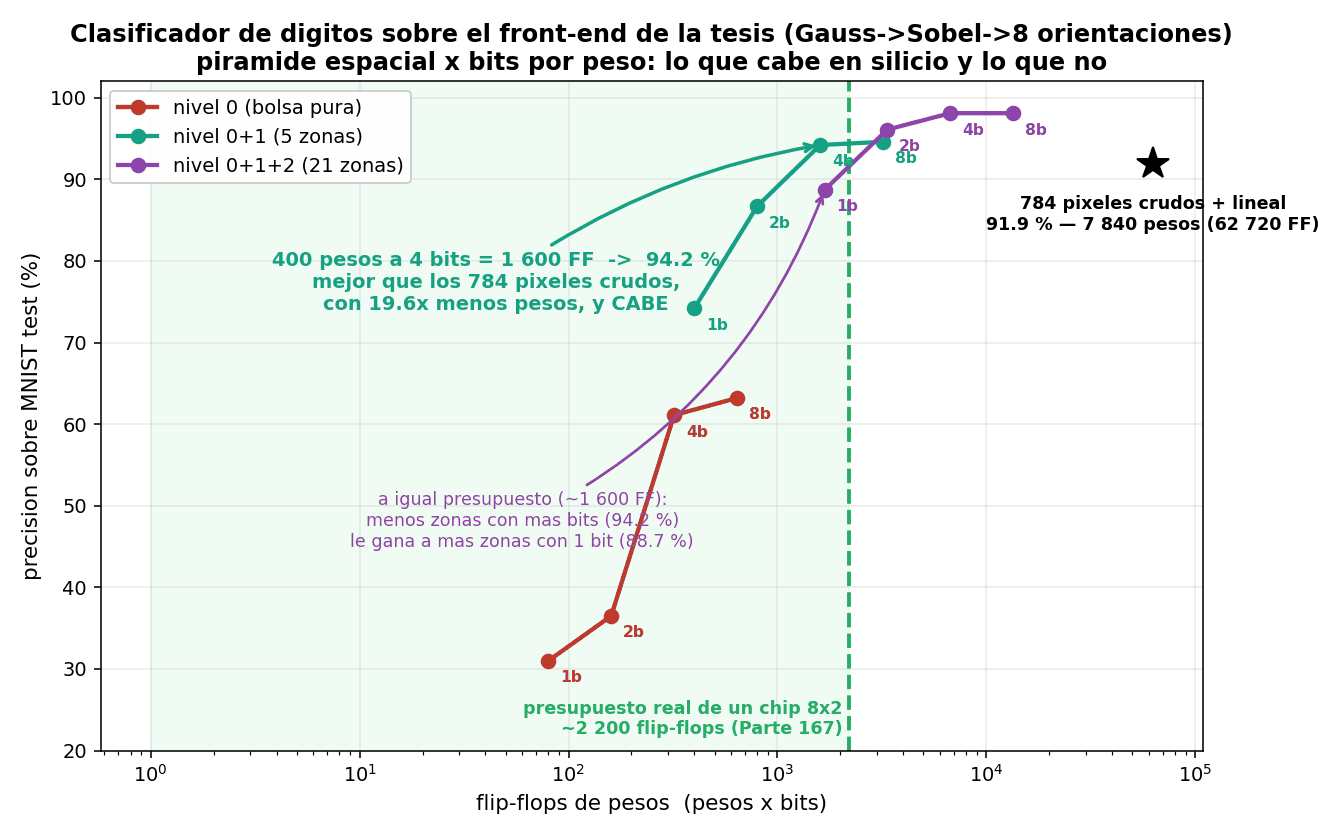
\includegraphics[keepaspectratio,alt={Figura 5.4. El espacio de diseño del clasificador, con el eje horizontal en escala logarítmica. Cada curva es un nivel de la pirámide espacial y cada punto una precisión de peso distinta. El hallazgo está en el cruce: 400 pesos de 4 bits ---1 600 biestables--- superan a los 784 píxeles crudos usando la vigésima parte de la memoria, y caben bajo el presupuesto real de un chip de 8×2 mosaicos, marcado con la línea vertical. A igualdad de memoria, la precisión de los pesos vale más que el número de zonas.}]{figuras/fig_5_4_espacio_de_diseno.png}}
\caption{\textbf{Figura 5.4.} El espacio de diseño del clasificador, con
el eje horizontal en escala logarítmica. Cada curva es un nivel de la
pirámide espacial y cada punto una precisión de peso distinta. El
hallazgo está en el cruce: \textbf{400 pesos de 4 bits ---1 600
biestables--- superan a los 784 píxeles crudos usando la vigésima parte
de la memoria}, y caben bajo el presupuesto real de un chip de 8×2
mosaicos, marcado con la línea vertical. A igualdad de memoria, la
precisión de los pesos vale más que el número de zonas.}
\end{figure}

\subsection{5.6.3 Lo que la exactitud no
muestra}\label{lo-que-la-exactitud-no-muestra}

Las medidas basadas en el \texttt{argmax} descartan la información de
los diez puntajes. Dos medidas que la conservan revelan una diferencia
que la exactitud oculta:

\begin{longtable}[]{@{}lrrr@{}}
\toprule\noalign{}
front-end & AUC macro & Brier & Brier skill \\
\midrule\noalign{}
\endhead
\bottomrule\noalign{}
\endlastfoot
SoC + Canny 1-salto & \textbf{0.9960} & \textbf{0.1465} &
\textbf{0.8371} \\
Canny 1-salto & 0.9957 & 0.1558 & 0.8268 \\
Sobel & 0.9945 & 0.1746 & 0.8059 \\
Canny transitivo & 0.9942 & \textbf{0.1991} & 0.7787 \\
SoC + Sobel & 0.9939 & 0.1749 & 0.8056 \\
\end{longtable}

El resultado de interés corresponde al Canny transitivo. En AUC ---que
mide el \textbf{ordenamiento}--- supera al SoC+Sobel; en Brier ---que
mide la \textbf{calibración}--- queda último por amplio margen.
\textbf{Ordena correctamente y decide mal.} Ello explica de forma
mecánica sus 139 falsos positivos: la reconstrucción morfológica
engruesa los contornos, el engrosamiento infla los histogramas, y el
criterio de rechazo ---que compara el mejor puntaje con el segundo---
deja hablar al circuito cuando debería callarlo.

\subsection{5.6.4 El punto de operación pesa más que el
front-end}\label{el-punto-de-operaciuxf3n-pesa-muxe1s-que-el-front-end}

Las comparaciones anteriores fijan el umbral y varían el filtro. El
experimento complementario ---fijar el filtro y \textbf{barrer el
umbral}--- arroja el resultado de mayor consecuencia práctica de esta
sección:

\begin{longtable}[]{@{}lrr@{}}
\toprule\noalign{}
magnitud & rango de exactitud & en unidades de σ \\
\midrule\noalign{}
\endhead
\bottomrule\noalign{}
\endlastfoot
el umbral, dentro del Sobel & \textbf{5.79 pp} & \textbf{4.4 σ} \\
el umbral, dentro del Canny & 0.90 pp & 0.7 σ \\
el filtro, cada uno en su óptimo & 0.38 pp & 0.3 σ \\
\end{longtable}

\textbf{Mover el umbral dentro del Sobel altera el resultado quince
veces más que cambiar de filtro.} Y la asimetría entre ambos front-ends
es el hallazgo: el Sobel presenta un óptimo estrecho ---su exactitud
recorre casi seis puntos a lo largo del rango útil--- mientras que el
Canny se mantiene en una meseta de nueve décimas. \textbf{El Canny en su
peor umbral supera al Sobel en diez de los once umbrales ensayados.}

El mecanismo reside en el algoritmo: el Sobel aplica un corte único y
nada recupera al píxel que queda por debajo; el Canny dispone de dos
umbrales y una histéresis que promueve el píxel débil adyacente a uno
fuerte. \textbf{La histéresis es un mecanismo de recuperación}, y de ahí
su insensibilidad.

\begin{quote}
\textbf{Consecuencia de diseño.} El front-end y el registro escribible
resuelven el mismo problema por vías distintas: el Canny adquiere
\textbf{en hardware} ---un \emph{line-buffer} adicional y ocho
comparaciones--- buena parte de la robustez que el Sobel obtiene
mediante \textbf{un procesador} capaz de reescribir el umbral. No son
decisiones que se sumen: son, en buena medida, \textbf{alternativas}.
\end{quote}

\subsection{5.6.5 El RTL contra el modelo, sobre el conjunto
completo}\label{el-rtl-contra-el-modelo-sobre-el-conjunto-completo}

Las cifras anteriores son del modelo en Python. La pregunta que decide
si sirven de algo es si el circuito las reproduce, y se respondió por el
camino más exigente disponible: \textbf{ejecutar el RTL sobre las diez
mil imágenes de prueba} en el simulador y comparar, no los porcentajes
agregados, sino cada predicción con la del modelo.

\begin{longtable}[]{@{}
  >{\raggedright\arraybackslash}p{(\linewidth - 2\tabcolsep) * \real{0.5000}}
  >{\raggedright\arraybackslash}p{(\linewidth - 2\tabcolsep) * \real{0.5000}}@{}}
\toprule\noalign{}
\begin{minipage}[b]{\linewidth}\raggedright
Comparación
\end{minipage} & \begin{minipage}[b]{\linewidth}\raggedright
Resultado
\end{minipage} \\
\midrule\noalign{}
\endhead
\bottomrule\noalign{}
\endlastfoot
Predicciones idénticas & \textbf{10 000 / 10 000} \\
Exactitud del RTL / del modelo & \textbf{91.04 \% / 91.04 \%} \\
Matriz de confusión & idéntica elemento por elemento \\
Veredictos de la clase de rechazo & \textbf{10 000 / 10 000}
idénticos \\
Cuadros aceptados · precisión al responder & 8 838 (88.38 \%) · 95.44
\%, en ambos \\
\end{longtable}

\begin{figure}
\centering
\pandocbounded{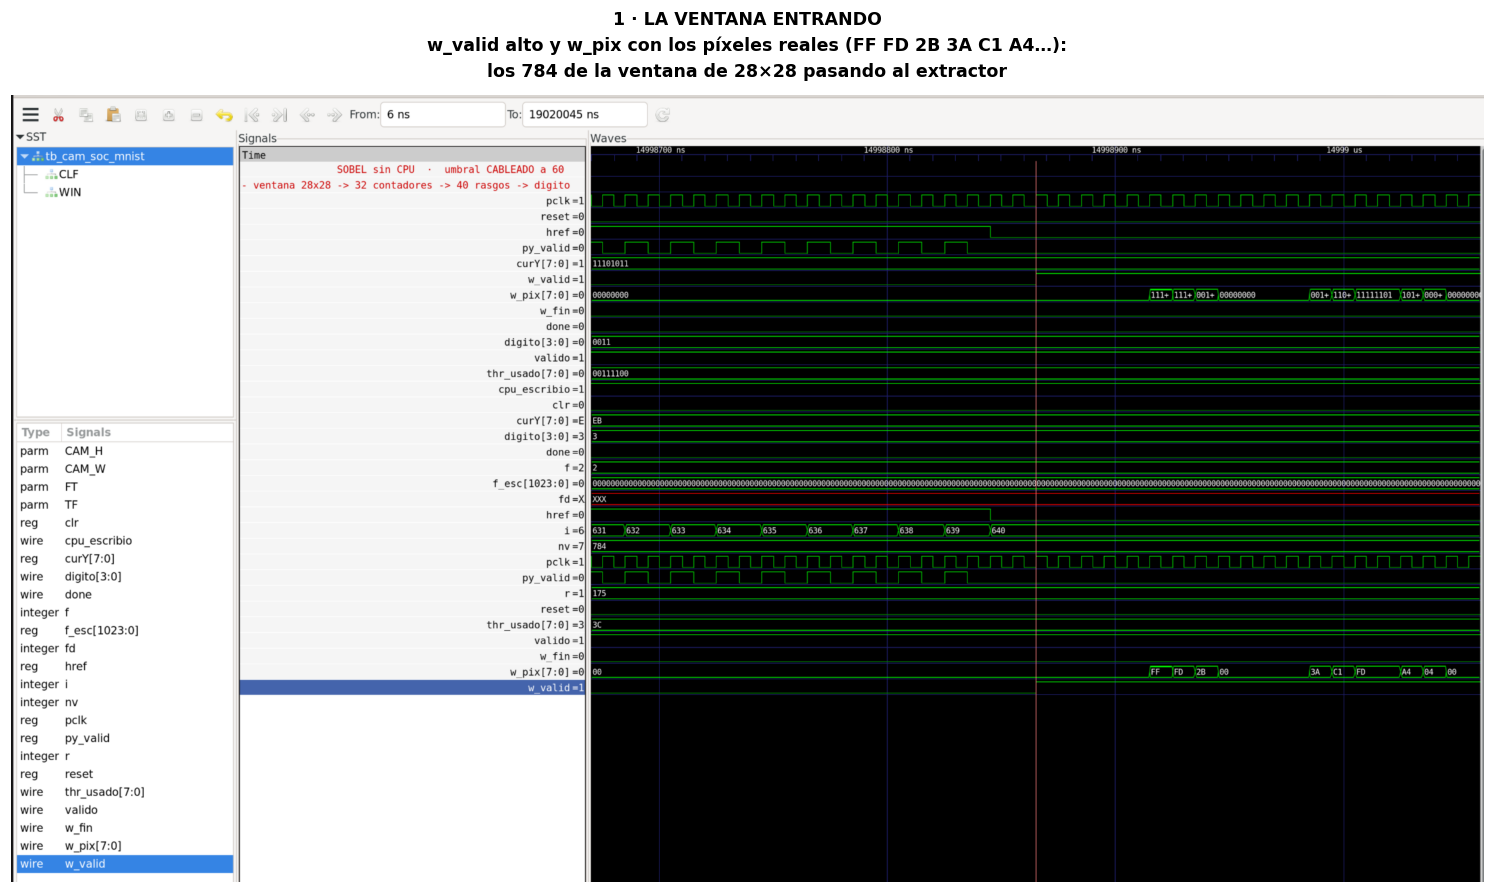
\includegraphics[keepaspectratio,alt={Figura 5.5. La ventana de 28×28 entrando al extractor, vista en el simulador. La señal w\_valid marca cada píxel válido y w\_pix lleva su valor ---FF FD 2B 3A C1 A4\ldots---; los 784 de la ventana pasan uno a uno antes de que done presente un dígito. Es el nivel al que se hizo la comparación contra el modelo: no se compararon porcentajes, se compararon señales.}]{figuras/fig_5_5_ventana_al_extractor.png}}
\caption{\textbf{Figura 5.5.} La ventana de 28×28 entrando al extractor,
vista en el simulador. La señal \texttt{w\_valid} marca cada píxel
válido y \texttt{w\_pix} lleva su valor
---\texttt{FF\ FD\ 2B\ 3A\ C1\ A4}\ldots---; los 784 de la ventana pasan
uno a uno antes de que \texttt{done} presente un dígito. Es el nivel al
que se hizo la comparación contra el modelo: no se compararon
porcentajes, se compararon señales.}
\end{figure}

No son cifras «parecidas» ni «dentro del margen de error»: \textbf{las
diez mil predicciones y los diez mil veredictos coinciden uno por uno},
y la matriz de confusión es la misma casilla por casilla. La
verificación de los filtros de la §5.1 se hizo sobre cinco imágenes;
ésta se hizo sobre diez mil, e incluye la decisión de rechazo, que es
lógica de comparación y no de aritmética.

\begin{quote}
Conviene precisar el alcance, porque más adelante aparece una cifra
distinta. Lo que aquí es exacto es el \textbf{clasificador completo}
---descriptor, pesos y decisión--- evaluado imagen por imagen. El 99.91
\% que informa la §5.6.6 se refiere a otra comparación: la del
\textbf{extractor de bordes} píxel a píxel dentro de la cadena, cuyas
discrepancias se concentran en la última fila del cuadro y no alteran
ninguna de las diez mil clasificaciones. Son dos medidas de objetos
distintos y no se contradicen.
\end{quote}

\subsection{5.6.6 Validación física}\label{validaciuxf3n-fuxedsica}

La validación sobre la placa se realizó en dos ensayos distintos, que
miden cosas distintas y cuyos resultados no deben confundirse.

\begin{figure}
\centering
\pandocbounded{
\includegraphics[keepaspectratio,alt={Figura 5.6. La cadena completa ---cámara, procesador, filtro y clasificador--- en señales, sobre la escena del dígito 3. El panel A muestra los 19 ms de dos cuadros: el veredicto sale en el primero y no cambia en el segundo. El panel B captura el instante en que el procesador sustituye el umbral por omisión del RTL, 110, por el 90 que escribe el firmware, con el camino de datos todavía en reinicio. El panel C mide los 639,5 µs que tardan las 400 multiplicaciones-acumulaciones y el argmax.}]{figuras/fig_5_6_cadena_en_senales.png}}
\caption{\textbf{Figura 5.6.} La cadena completa ---cámara, procesador,
filtro y clasificador--- en señales, sobre la escena del dígito 3. El
panel A muestra los 19 ms de dos cuadros: el veredicto sale en el
primero y no cambia en el segundo. El panel B captura el instante en que
\textbf{el procesador sustituye el umbral por omisión del RTL, 110, por
el 90 que escribe el firmware}, con el camino de datos todavía en
reinicio. El panel C mide los 639,5 µs que tardan las 400
multiplicaciones-acumulaciones y el \texttt{argmax}.}
\end{figure}

\textbf{Primer ensayo: diez dígitos grabados en el propio bitstream.} Se
embebieron diez imágenes de MNIST en la memoria de configuración y se
hizo que el circuito informara sus veredictos por el puerto serie, sin
cámara. La placa acertó \textbf{ocho de los diez}, y lo relevante no son
los ocho aciertos sino los dos fallos: el circuito confunde el
\textbf{2} con un 0 y el \textbf{3} con un 8, \textbf{exactamente los
mismos dos dígitos y exactamente las mismas respuestas equivocadas} que
había dado la simulación del diseño completo. Ninguno de los diez cambió
de respuesta a lo largo de unas treinta repeticiones.

\begin{quote}
Reproducir un acierto puede ser casualidad; reproducir un error
específico y repetido, no. Este ensayo no mide la exactitud del sistema
---diez imágenes no son una medida estadística--- sino que
\textbf{cierra el último eslabón de la traducción}: el diseño
sintetizado, emplazado, ruteado y cargado en silicio se comporta como el
RTL verificado, errores incluidos.
\end{quote}

\begin{figure}
\centering
\pandocbounded{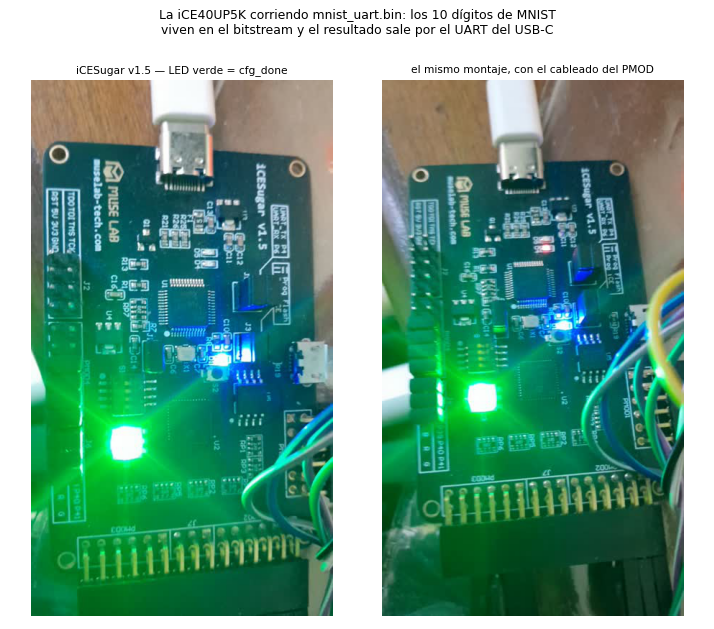
\includegraphics[keepaspectratio,alt={Figura 5.7. La tarjeta durante ese primer ensayo, con el mapa de bits cargado. El diodo verde está cableado a la señal de configuración terminada; el azul parpadea con el latido del sistema. Los diez veredictos salen por el puerto serie del mismo conector que alimenta la tarjeta. A la derecha, el mismo montaje con el cableado del módulo de pantalla ya conectado.}]{figuras/fig_5_7_la_placa_uart.png}}
\caption{\textbf{Figura 5.7.} La tarjeta durante ese primer ensayo, con
el mapa de bits cargado. El diodo verde está cableado a la señal de
configuración terminada; el azul parpadea con el latido del sistema. Los
diez veredictos salen por el puerto serie del mismo conector que
alimenta la tarjeta. A la derecha, el mismo montaje con el cableado del
módulo de pantalla ya conectado.}
\end{figure}

\textbf{Segundo ensayo: dígitos manuscritos ante la cámara.} El sistema
completo ---procesador RISC-V, periférico de umbrales, front-end Canny y
clasificador--- se enfrentó a dígitos escritos a mano y captados por una
cámara OV7670. \textbf{El circuito reconoció nueve de diez dígitos},
coincidiendo exactamente con lo que la simulación había predicho para
esa configuración.

Ese acuerdo, sin embargo, no se obtuvo al primer intento, y la causa
merece registrarse porque es la única discrepancia entre simulación y
silicio de todo el trabajo. En la primera versión la placa respondía
\textbf{ocho de diez} mientras la simulación sostenía nueve. El umbral
inferior del front-end se leía desde el módulo de control mediante una
\textbf{referencia jerárquica} ---\texttt{SOC.flt\_tlo}--- en lugar de
un puerto declarado. Ambas herramientas aceptaron el archivo sin una
sola advertencia y construyeron circuitos distintos: \texttt{iverilog}
resuelve la referencia y simula con el umbral escrito por el procesador,
mientras que el sintetizador crea un cable implícito de un bit que nadie
gobierna y fija el umbral inferior en cero. Sustituida la referencia por
un \textbf{puerto real}, la placa pasó a nueve de diez: el valor que la
simulación predecía.

\begin{quote}
\textbf{La lección no es que hubiera un error, sino dónde estaba.} El
RTL era legal, la simulación era correcta y la síntesis también lo era;
lo que falló fue suponer que ambas leían la misma descripción. Una
construcción que el lenguaje admite y que las dos herramientas
interpretan de forma distinta es indetectable por inspección y
silenciosa en los registros de ambas. Se deja escrita la regla de
trabajo que se adoptó a partir de aquí: \textbf{toda señal que cruce una
frontera de módulo se declara como puerto}, aunque el simulador acepte
el atajo.
\end{quote}

La verificación del extractor contra su modelo de referencia arrojó
\textbf{99.91 \%} de coincidencia exacta píxel a píxel para el Sobel y
\textbf{99.93 \%} para el Canny, concentrándose las diferencias en la
última fila del cuadro.

\subsection{5.6.7 Implementación en
silicio}\label{implementaciuxf3n-en-silicio}

El reconocedor se llevó a tecnología \texttt{sky130\_fd\_sc\_hd} en dos
variantes, ejecutando el flujo completo de OpenLane hasta la firma del
GDS:

\begin{longtable}[]{@{}lrr@{}}
\toprule\noalign{}
magnitud & Sobel & Canny 1-salto \\
\midrule\noalign{}
\endhead
\bottomrule\noalign{}
\endlastfoot
área del \emph{die} & 0.845 mm² & 0.890 mm² \\
celdas tras síntesis & 16 718 & 17 373 \\
celdas emplazadas & 19 949 & 20 921 \\
período de reloj & 30 ns (33.3 MHz) & 30 ns (33.3 MHz) \\
holgura con parásitos (\texttt{spef\_wns}) & \textbf{0.00 ns} &
\textbf{0.00 ns} \\
DRC · LVS · XOR & 0 · 0 · 0 & 0 · 0 · 0 \\
\end{longtable}

Ambos circuitos cierran el temporizado con los parásitos del
interconexionado extraídos y superan las tres verificaciones de firma
sin observaciones. Merece señalarse que \textbf{cierran más rápido que
los circuitos de visión equivalentes} ---que requirieron 32 y 36 ns---,
lo que resulta coherente con la ausencia de memoria de cuadro: es el
multiplexor de lectura del \emph{framebuffer} el que constituye el
camino crítico de aquéllos.

\textbf{Son los primeros circuitos de este trabajo cuya salida no es una
imagen.} Los diez presentados en las secciones §5.3 y §5.4 procesan;
éstos reconocen.

\subsection{5.6.8 El costo relativo del front-end depende del
sistema}\label{el-costo-relativo-del-front-end-depende-del-sistema}

La comparación de área entre ambos front-ends admite cuatro niveles de
integración. Las cuatro filas están en \textbf{celdas emplazadas}, la
misma escala de la §5.3, de modo que los cocientes son directamente
comparables entre sí:

\begin{longtable}[]{@{}
  >{\raggedright\arraybackslash}p{(\linewidth - 6\tabcolsep) * \real{0.2000}}
  >{\raggedleft\arraybackslash}p{(\linewidth - 6\tabcolsep) * \real{0.2667}}
  >{\raggedleft\arraybackslash}p{(\linewidth - 6\tabcolsep) * \real{0.2667}}
  >{\raggedleft\arraybackslash}p{(\linewidth - 6\tabcolsep) * \real{0.2667}}@{}}
\toprule\noalign{}
\begin{minipage}[b]{\linewidth}\raggedright
nivel
\end{minipage} & \begin{minipage}[b]{\linewidth}\raggedleft
Sobel
\end{minipage} & \begin{minipage}[b]{\linewidth}\raggedleft
Canny
\end{minipage} & \begin{minipage}[b]{\linewidth}\raggedleft
factor
\end{minipage} \\
\midrule\noalign{}
\endhead
\bottomrule\noalign{}
\endlastfoot
filtro aislado & 5 823 & 12 993 & \textbf{2.23×} \\
con procesador & 12 043 & 22 054 & 1.83× \\
sistema de visión completo & 35 653 & 41 925 & 1.18× \\
reconocedor con procesador & 19 949 & 20 921 & 1.05× \\
\textbf{reconocedor que además muestra} & \textbf{38 643} & \textbf{39
794} & \textbf{1.03×} \\
\end{longtable}

\textbf{El sobrecosto del Canny se diluye conforme crece el sistema que
lo rodea.} Considerado de forma aislada cuesta un \textbf{123 \%} más;
con un procesador al lado, un 83 \%; dentro de un sistema de visión, un
18 \%; integrado en un reconocedor, un 5 \%; y en un reconocedor que
además dibuja en pantalla, un \textbf{3 \%}. El motivo es que el
clasificador ---histograma, pirámide y 400 multiplicaciones--- es
idéntico en ambas variantes y domina el área, mientras que la diferencia
se reduce al tercer \emph{line-buffer}.

De ello se sigue una conclusión condicional: \textbf{el Sobel aventaja
al Canny en área únicamente cuando el filtro constituye el circuito
completo.} En un sistema que reconoce, esa ventaja ---la única que el
Sobel conserva, según §5.6.2 a §5.6.4--- deja de ser determinante.

\begin{center}\rule{0.5\linewidth}{0.5pt}\end{center}

\subsection{Referencias de la
sección}\label{referencias-de-la-secciuxf3n}

\begin{itemize}
\tightlist
\item
  Chow, C. K. (1970). \emph{On Optimum Recognition Error and Reject
  Tradeoff.} IEEE Trans. Inf. Theory, 16(1), 41-46.
\item
  Dalal, N. y Triggs, B. (2005). \emph{Histograms of Oriented Gradients
  for Human Detection.} CVPR, 886-893.
\item
  Lazebnik, S., Schmid, C. y Ponce, J. (2006). \emph{Beyond Bags of
  Features: Spatial Pyramid Matching.} CVPR, 2169-2178.
\item
  Lowe, D. G. (2004). \emph{Distinctive Image Features from
  Scale-Invariant Keypoints.} IJCV, 60(2), 91-110.
\end{itemize}

\section{5.7 Verificación eléctrica del camino
crítico}\label{verificaciuxf3n-eluxe9ctrica-del-camino-cruxedtico}

\begin{quote}
\textbf{Estado:} borrador 1, 2026-09-21. Fuente: cuaderno 2, §33. Todas
las cifras de esta sección proceden de corridas de NGSpice sobre
\texttt{sky130\_fd\_sc\_hd} en la esquina típica, 1,8 V y 25 °C, y de
los ficheros de parásitos extraídos de los dos reconocedores.
\end{quote}

Las secciones anteriores aceptaron sin discusión lo que el analizador de
tiempos informa. Ésta pregunta si ese número es correcto, y lo hace por
el único camino que no depende de la misma herramienta: \textbf{resolver
los transistores}.

La pregunta no es ociosa. Un analizador estático no simula: consulta
tablas caracterizadas de antemano e interpola. Es rapidísimo y es lo que
permite firmar un circuito de doscientas mil instancias, pero entre su
respuesta y la física median un modelo de celda, un modelo de cable y un
procedimiento de interpolación. Comprobar cuánto de lo que informa
sobrevive a una simulación eléctrica es, por tanto, una verificación del
instrumento y no del circuito.

\subsection{5.7.1 Por qué el camino crítico y no el
chip}\label{por-quuxe9-el-camino-cruxedtico-y-no-el-chip}

Simular los dos reconocedores enteros no es inviable por tamaño
---\texttt{pan\_sobel} tiene 116 314 transistores y en este trabajo ya
se simuló un procesador de 121 310--- sino \textbf{por tiempo}: para que
el clasificador vea sus 784 píxeles hay que hacerle entrar un cuadro
completo, y eso son 633 800 ciclos, unos treinta y dos veces más
actividad que la simulación de procesador ya realizada.

El camino crítico, en cambio, son \textbf{treinta y siete celdas} en un
chip y treinta y seis en el otro. Se extrajeron del reporte del
analizador, se reconstruyeron como cadena aislada con la carga y la
pendiente que el propio reporte declara en cada etapa, y se resolvieron
en NGSpice.

\subsection{5.7.2 El resultado}\label{el-resultado}

Se aplicaron cinco variantes del mismo banco, cada una añadiendo un
ingrediente al anterior, de modo que la diferencia entre dos renglones
consecutivos aísla la contribución de ese ingrediente:

\begin{longtable}[]{@{}
  >{\raggedright\arraybackslash}p{(\linewidth - 4\tabcolsep) * \real{0.2727}}
  >{\raggedleft\arraybackslash}p{(\linewidth - 4\tabcolsep) * \real{0.3636}}
  >{\raggedleft\arraybackslash}p{(\linewidth - 4\tabcolsep) * \real{0.3636}}@{}}
\toprule\noalign{}
\begin{minipage}[b]{\linewidth}\raggedright
\end{minipage} & \begin{minipage}[b]{\linewidth}\raggedleft
\texttt{pan\_sobel} (37 etapas)
\end{minipage} & \begin{minipage}[b]{\linewidth}\raggedleft
\texttt{pan\_canny} (36 etapas)
\end{minipage} \\
\midrule\noalign{}
\endhead
\bottomrule\noalign{}
\endlastfoot
\textbf{Analizador estático, con parásitos} & \textbf{12,230 ns} &
\textbf{9,890 ns} \\
A · las puertas solas & 4,646 ns & 4,424 ns \\
B · más la capacitancia extraída, agrupada & 8,159 ns & 7,552 ns \\
C · más la pendiente de entrada real & 8,178 ns & 7,588 ns \\
D0 · más la topología del fichero de parásitos, \textbf{con R = 0} &
7,603 ns & 7,022 ns \\
D · más la \textbf{resistencia medida} de cada tramo & 7,620 ns & 7,043
ns \\
E · más la \textbf{celda extraída del \emph{layout}} & \textbf{9,694 ns}
& \textbf{8,962 ns} \\
\emph{fracción del retardo que la simulación reproduce} & \emph{79,3 \%}
& \emph{90,6 \%} \\
\end{longtable}

La variante \textbf{D0 es un control}, idéntica a la D salvo en que sus
resistencias valen cero. Sin ella, el efecto de la resistencia y el de
\emph{repartir} la capacitancia a lo largo del árbol en vez de agruparla
en un nodo quedarían sumados en una sola cifra y no podrían separarse.

\begin{figure}
\centering
\pandocbounded{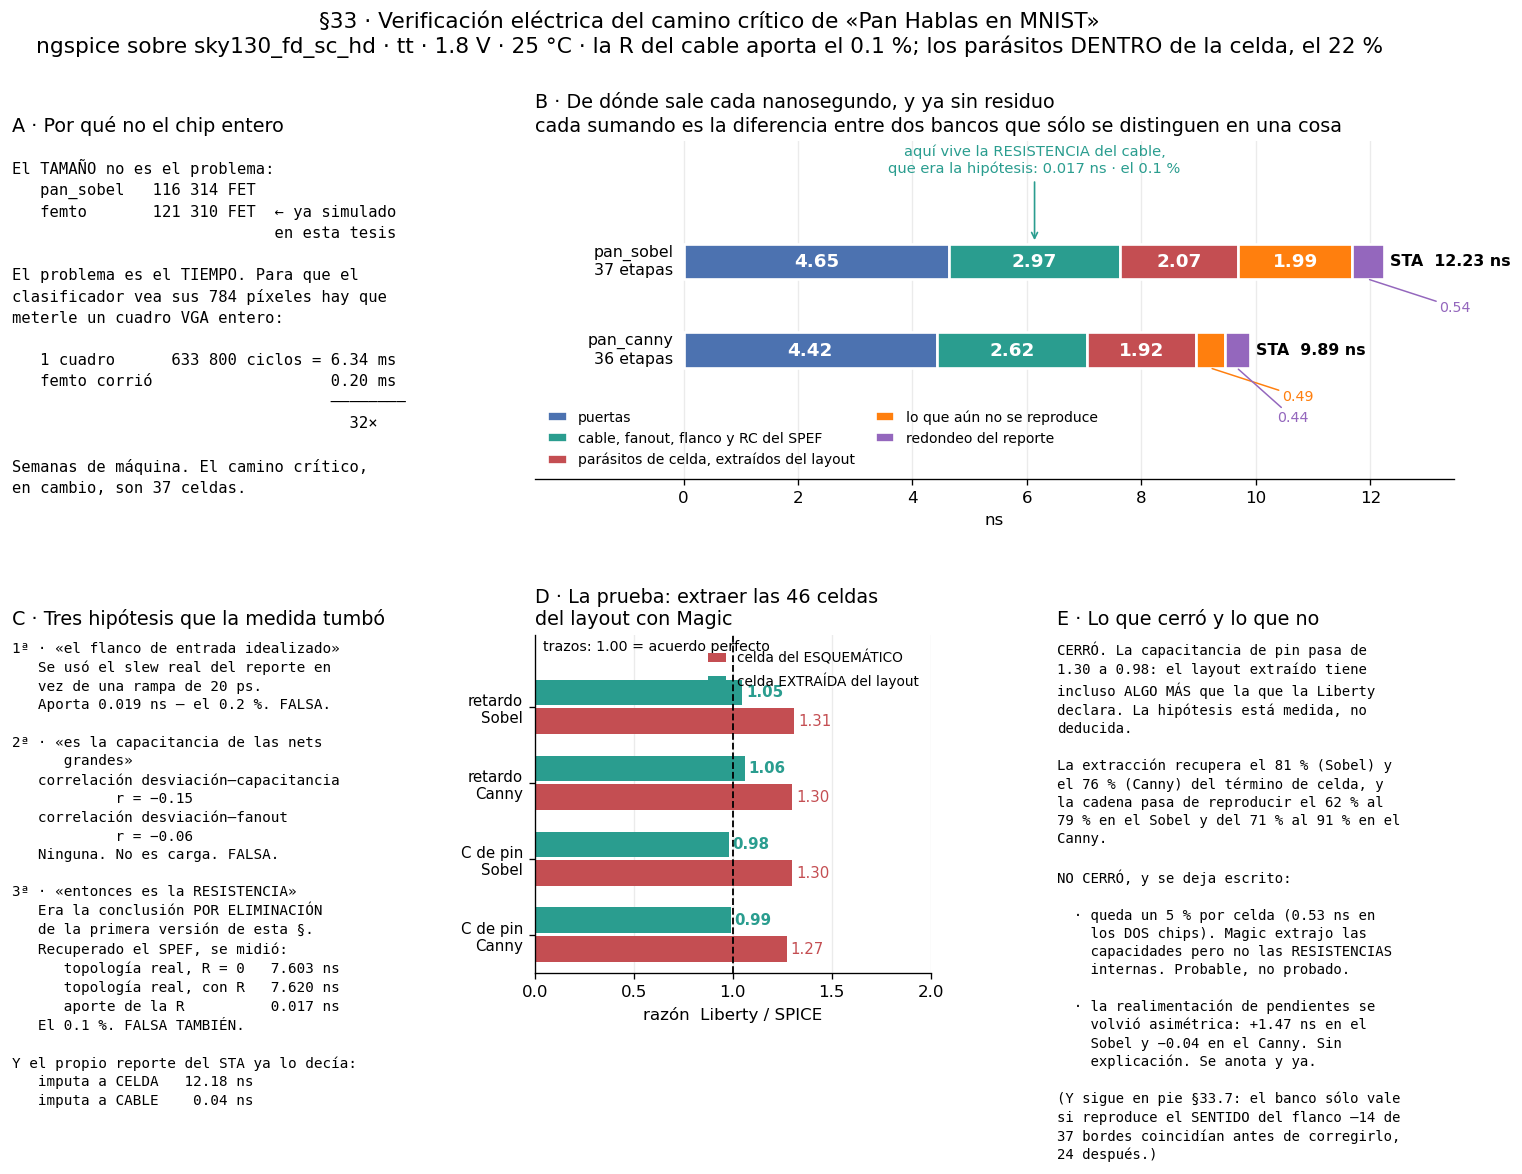
\includegraphics[keepaspectratio,alt={Figura 5.8. El desglose completo de la verificación. El panel A explica por qué se simula el camino y no el chip; el B reparte los 12,23 ns del pan\_sobel y los 9,89 del pan\_canny en sumandos que no dejan residuo; el C recoge las tres hipótesis que la medida desmintió; el D contrapone la celda del esquemático con la extraída del dibujo en los dos experimentos independientes; y el E separa lo que quedó cerrado de lo que se deja escrito como abierto.}]{figuras/fig_5_8_spice_desglose.png}}
\caption{\textbf{Figura 5.8.} El desglose completo de la verificación.
El panel A explica por qué se simula el camino y no el chip; el B
reparte los 12,23 ns del \texttt{pan\_sobel} y los 9,89 del
\texttt{pan\_canny} en sumandos que no dejan residuo; el C recoge las
tres hipótesis que la medida desmintió; el D contrapone la celda del
esquemático con la extraída del dibujo en los dos experimentos
independientes; y el E separa lo que quedó cerrado de lo que se deja
escrito como abierto.}
\end{figure}

\subsection{5.7.3 Tres explicaciones que la medida
desmintió}\label{tres-explicaciones-que-la-medida-desmintiuxf3}

Las tres parecían razonables, y conviene dejar constancia de las tres.

\textbf{El flanco de entrada idealizado.} El estímulo inicial era una
rampa de 20 ps, mucho más limpia que la transición que la primera etapa
recibe en el circuito; cabía esperar que un frente degradado se
propagase como retardo a lo largo de las treinta y siete etapas.
Sustituido por la pendiente real que el reporte declara, la contribución
resultó de \textbf{0,019 ns: el 0,2 \%}.

\textbf{La capacitancia de las redes grandes.} Las desviaciones mayores
se concentraban en puertas de muchas entradas, lo que sugería redes
largas y cargadas. Se midió la correlación entre la desviación de cada
etapa y su capacitancia: \textbf{r = −0,15}; y con el número de
destinos: \textbf{r = −0,06}. Ninguna de las dos sostiene la
explicación.

\textbf{La resistencia de la interconexión.} Descartadas las anteriores
quedaba ésta, y \textbf{así se dio por concluida la primera versión de
esta sección}: el analizador trabaja sobre el fichero de parásitos, que
informa resistencia y capacitancia de cada red, mientras que el reporte
de texto publica sólo la capacitancia, de modo que la simulación habría
recibido una descripción incompleta de los cables. La conjetura no pudo
comprobarse entonces porque ese fichero no se había conservado.

Recuperado, se midió. \textbf{La resistencia de la interconexión aporta
0,017 ns: el 0,1 \% del camino.} No los cuatro nanosegundos que había
que explicar.

\begin{quote}
\textbf{El propio reporte lo decía, y no se leyó.} El analizador imputa
cada retardo a un pin, y los de pin de salida son de celda mientras que
los de pin de entrada son de cable. Sumados por separado a lo largo del
camino: \textbf{12,18 ns imputados a celda y 0,04 ns a cable}. La
herramienta nunca atribuyó el tiempo a la interconexión. Bastaba con
sumar dos columnas.
\end{quote}

\subsection{5.7.4 La causa: la celda del esquemático no es la celda del
silicio}\label{la-causa-la-celda-del-esquemuxe1tico-no-es-la-celda-del-silicio}

Si la diferencia está dentro de las celdas, hay que preguntárselo a una
celda sola. El banco se redujo al mínimo ---una celda, el arco que el
camino recorre, la pendiente y la carga que el reporte declara--- y se
hizo la misma pregunta dos veces: a la tabla caracterizada, interpolando
como hace el analizador, y al simulador, resolviendo los transistores
que el kit de diseño distribuye.

La tabla reproduce al analizador casi exactamente, lo que confirma que
éste se limita a consultarla. La simulación, en cambio, queda
\textbf{sistemáticamente por debajo en treinta y cinco de las treinta y
siete etapas}, con una razón de \textbf{1,31} que no depende ni de la
carga ni de la pendiente. Esa independencia es la que descarta un
defecto del banco y señala a la celda misma.

La causa está en el fichero que se le entregó como modelo. El kit
distribuye el netlist \textbf{esquemático}: doce transistores y ni un
solo parásito. La biblioteca caracterizada, en cambio, se obtuvo sobre
la celda \textbf{dibujada}, con el metal, los contactos y la difusión
que el \emph{layout} añade. Al simulador se le describió la celda antes
de dibujarla.

Eso admite medición directa. Inyectando una rampa lenta en cada pin de
entrada e integrando la corriente ---capacitancia como carga dividida
por tensión, sin modelo ni supuesto--- la biblioteca atribuye a cada
pin, en promedio sobre los treinta y cinco del camino, \textbf{un 30 \%
más de capacitancia de la que el esquemático tiene}.

\begin{quote}
\textbf{Dos experimentos distintos, la misma cifra.} La razón entre el
retardo que la biblioteca declara y el que la simulación obtiene sobre
el esquemático es \textbf{1,31}. La razón entre la capacitancia que la
biblioteca declara y la que el esquemático tiene es \textbf{1,30}. Uno
mide tiempos y el otro mide carga, sobre las mismas treinta y siete
etapas.
\end{quote}

\textbf{La comprobación.} Lo anterior establece que al esquemático le
faltan parásitos, no que sean \emph{ésos} los que faltan. El kit no
distribuye el netlist de la celda dibujada, pero sí el dibujo: se
extrajeron con Magic las \textbf{cuarenta y seis celdas} que aparecen en
los dos caminos y se repitieron los dos experimentos sin cambiar nada
más.

\begin{longtable}[]{@{}
  >{\raggedright\arraybackslash}p{(\linewidth - 4\tabcolsep) * \real{0.2727}}
  >{\raggedleft\arraybackslash}p{(\linewidth - 4\tabcolsep) * \real{0.3636}}
  >{\raggedleft\arraybackslash}p{(\linewidth - 4\tabcolsep) * \real{0.3636}}@{}}
\toprule\noalign{}
\begin{minipage}[b]{\linewidth}\raggedright
razón biblioteca / simulación
\end{minipage} & \begin{minipage}[b]{\linewidth}\raggedleft
celda del \textbf{esquemático}
\end{minipage} & \begin{minipage}[b]{\linewidth}\raggedleft
celda \textbf{extraída}
\end{minipage} \\
\midrule\noalign{}
\endhead
\bottomrule\noalign{}
\endlastfoot
capacitancia de pin · \texttt{pan\_sobel} & 1,30 & \textbf{0,98} \\
capacitancia de pin · \texttt{pan\_canny} & 1,27 & \textbf{0,99} \\
retardo de celda aislada · \texttt{pan\_sobel} & 1,31 & \textbf{1,05} \\
retardo de celda aislada · \texttt{pan\_canny} & 1,30 & \textbf{1,06} \\
\end{longtable}

\textbf{La discrepancia de capacitancia desaparece.} La hipótesis queda
medida y no deducida, que era justamente lo que faltaba.

\subsection{5.7.5 La cuenta, y lo que queda
abierto}\label{la-cuenta-y-lo-que-queda-abierto}

Repartidos los 12,230 ns sin residuo, el término que importa sale igual
en los dos circuitos:

\begin{longtable}[]{@{}
  >{\raggedright\arraybackslash}p{(\linewidth - 4\tabcolsep) * \real{0.2727}}
  >{\raggedleft\arraybackslash}p{(\linewidth - 4\tabcolsep) * \real{0.3636}}
  >{\raggedleft\arraybackslash}p{(\linewidth - 4\tabcolsep) * \real{0.3636}}@{}}
\toprule\noalign{}
\begin{minipage}[b]{\linewidth}\raggedright
\end{minipage} & \begin{minipage}[b]{\linewidth}\raggedleft
\texttt{pan\_sobel}
\end{minipage} & \begin{minipage}[b]{\linewidth}\raggedleft
\texttt{pan\_canny}
\end{minipage} \\
\midrule\noalign{}
\endhead
\bottomrule\noalign{}
\endlastfoot
\textbf{el modelo de celda, como fracción del camino} & \textbf{22,6 \%}
& \textbf{22,1 \%} \\
resistencia de la interconexión & 0,1 \% & 0,2 \% \\
\end{longtable}

Dos circuitos distintos, dos caminos críticos que no comparten una sola
instancia, y la misma cifra a cuatro décimas de punto: \textbf{algo más
de la quinta parte del retardo de un camino crítico la ponen los
parásitos que el dibujo añade dentro de las celdas.}

\begin{figure}
\centering
\pandocbounded{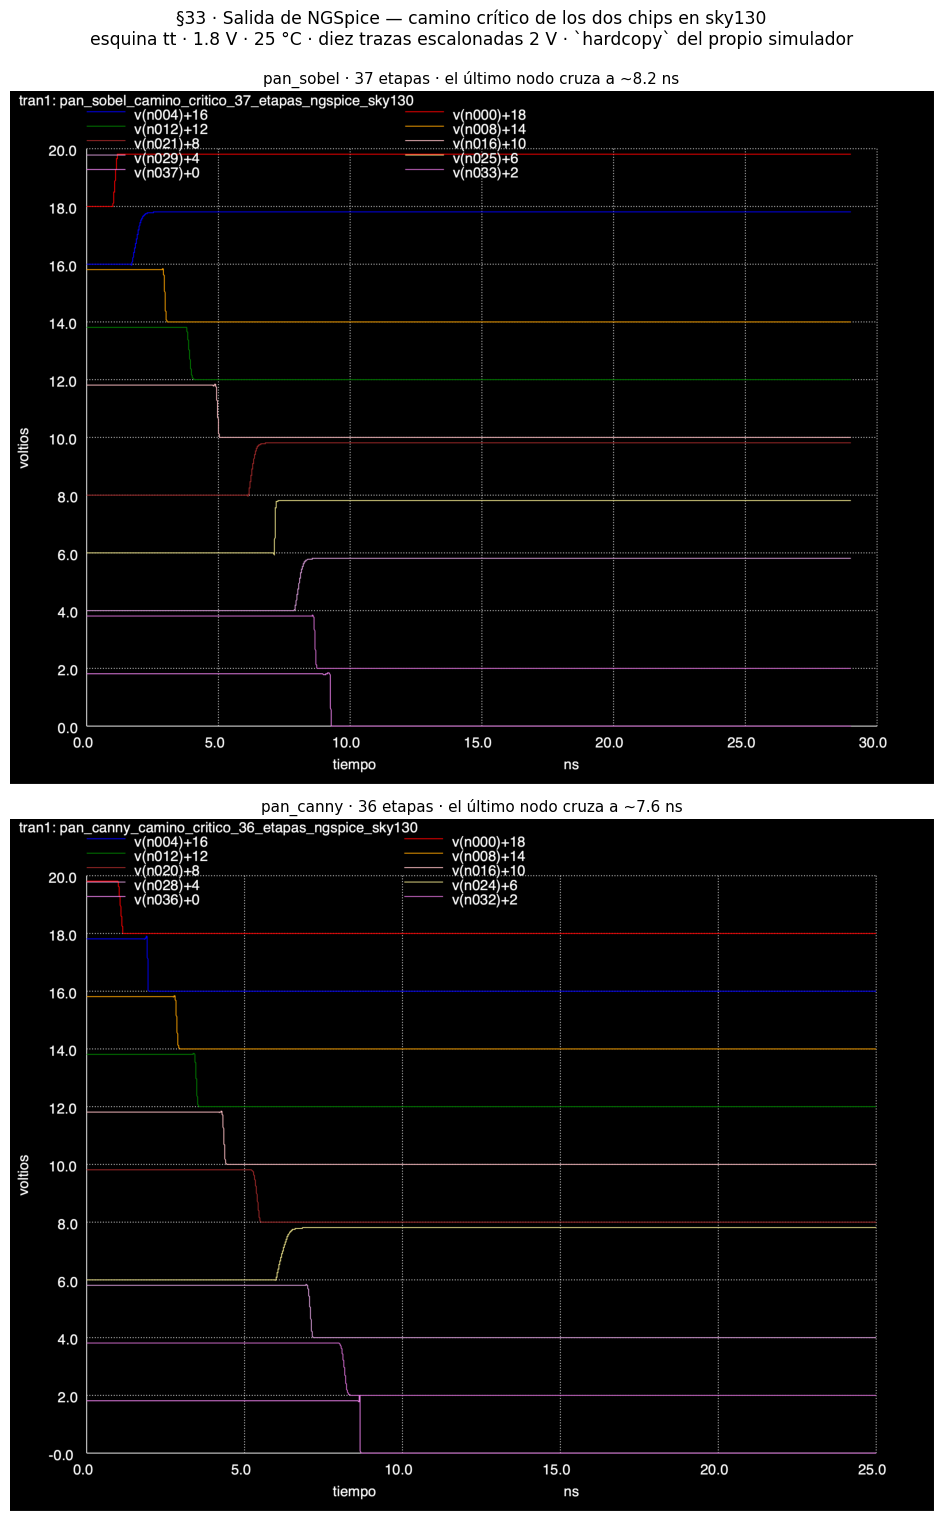
\includegraphics[keepaspectratio,alt={Figura 5.9. La salida del simulador, tal como éste la dibuja. Cada traza es un nodo del camino crítico, desplazada dos voltios respecto de la anterior para que las diez quepan en el mismo eje; la cascada de transiciones de arriba abajo es la señal propagándose etapa por etapa. El último nodo del pan\_sobel conmuta a unos 8,2 ns y el del pan\_canny a unos 7,6, que son las variantes D de la tabla anterior.}]{figuras/fig_5_9_spice_ondas.png}}
\caption{\textbf{Figura 5.9.} La salida del simulador, tal como éste la
dibuja. Cada traza es un nodo del camino crítico, desplazada dos voltios
respecto de la anterior para que las diez quepan en el mismo eje; la
cascada de transiciones de arriba abajo es la señal propagándose etapa
por etapa. El último nodo del \texttt{pan\_sobel} conmuta a unos 8,2 ns
y el del \texttt{pan\_canny} a unos 7,6, que son las variantes D de la
tabla anterior.}
\end{figure}

\textbf{Lo que no cerró, y se deja escrito.} Queda un 5 \% por celda
---0,528 ns en un chip y 0,530 en el otro, prácticamente el mismo valor
absoluto en dos caminos distintos--- que la extracción no recupera. La
explicación más probable es que el procedimiento empleado conserva las
\textbf{capacidades} internas de la celda pero no sus
\textbf{resistencias}, de modo que su metal interno sigue comportándose
como un cortocircuito ideal. Se anota como \textbf{probable y no
comprobada}. Y la realimentación de pendientes a lo largo de la cadena
resulta asimétrica entre los dos chips ---+1,47 ns en uno y −0,04 en el
otro--- sin explicación disponible.

\begin{quote}
\textbf{La conclusión.} El simulador y el analizador no discrepan sobre
la física: discrepan sobre el circuito. Al analizador se le describió la
celda tal como quedó en el \emph{layout}; al simulador, tal como estaba
en el esquema.

La verificación eléctrica no midió, por tanto, que el analizador se
equivocara. Midió \textbf{cuánto del retardo de un circuito integrado lo
pone el dibujo y no el esquema}: algo más de la quinta parte, y la misma
fracción en dos chips independientes. Es una cifra más útil que la que
se buscaba, y explica por qué ninguna implementación puede firmarse
sobre el esquemático.
\end{quote}

\chapter{6. Discusión}\label{discusiuxf3n}

\begin{quote}
\textbf{Estado:} borrador 1, escrito el 2026-09-21. Fuente: cuadernos 1
y 2, y el Capítulo 5. Formato Markdown para convertir con
\texttt{pandoc}.
\end{quote}

El capítulo anterior presentó mediciones. Éste sostiene afirmaciones. La
diferencia importa: una medición es un hecho que se comprueba repitiendo
el experimento, mientras que una afirmación es una lectura de varios
hechos y puede ser equivocada aunque todos ellos sean correctos. Este
trabajo tuvo que retractar dos afirmaciones de ese tipo durante su
desarrollo, y la experiencia dejó una disciplina que se aplica aquí:
\textbf{cada tesis de este capítulo señala qué medición la sostiene y
qué otra lectura descarta.}

\section{6.1 Lo que decide si un algoritmo cabe no es el
algoritmo}\label{lo-que-decide-si-un-algoritmo-cabe-no-es-el-algoritmo}

Ésta es la afirmación central del trabajo, y la más contraintuitiva para
quien llega desde el software.

Los tres filtros implementados ejecutan aritmética comparable. Ninguno
multiplica; los tres recorren la imagen aplicando una ventana de 3×3 y
comparando contra un umbral. Si el costo en silicio siguiera a la
complejidad aritmética, los tres deberían costar aproximadamente lo
mismo. La §5.4.3 midió lo contrario:

\begin{longtable}[]{@{}llr@{}}
\toprule\noalign{}
desde & hasta & cuesta \\
\midrule\noalign{}
\endhead
\bottomrule\noalign{}
\endlastfoot
Sobel & Canny de un salto & \textbf{+5 851 celdas} \\
Canny de un salto & Canny transitivo & \textbf{+94 511 celdas} \\
\end{longtable}

Ampliar el alcance de la ventana en un salto cuesta menos de seis mil
celdas. Ampliarlo al cuadro completo cuesta \textbf{noventa y cuatro mil
quinientas once}. Y la causa no está en las operaciones sino en
\textbf{cuánto estado hay que sostener a la vez}: los dos primeros
filtros procesan en flujo y retienen unas pocas líneas; el tercero
necesita el cuadro entero residente y accesible en orden arbitrario,
porque su punto fijo puede propagar una decisión desde cualquier píxel
hacia cualquier otro.

La comparación que resume el capítulo es ésta: \textbf{un procesador
RISC-V completo, con su memoria de programa y su periférico, cuesta
alrededor de nueve mil celdas} ---medido tres veces, sobre los tres
filtros, con una dispersión inferior al 5 \%--- \textbf{es decir,
aproximadamente la décima parte de lo que cuesta cambiar el alcance del
patrón de local a global.}

\begin{quote}
Dicho de otro modo: en el presupuesto de este chip, \textbf{meter un
procesador entero es una decisión menor comparada con decidir cuánta
imagen mira el filtro}. Es exactamente lo contrario de lo que sugiere la
intuición formada en software, donde el procesador es el recurso caro y
la memoria se pide al sistema operativo.
\end{quote}

\subsection{Las tres caras del mismo
precio}\label{las-tres-caras-del-mismo-precio}

El costo de la memoria no se cobra sólo en área. La §5.4.1 muestra que
\textbf{los dos circuitos transitivos son también los dos únicos que no
cierran temporizado}, con −19,35 ns y −18,23 ns de holgura una vez
extraídos los parásitos. El multiplexor que lee un framebuffer de miles
de entradas es un camino largo por construcción, y a partir de cierto
tamaño deja de ser caro para volverse inviable.

Y se cobra en manufacturabilidad. La §5.3 documenta que los diseños con
framebuffer grande acumulan un número de violaciones de antena muy
superior al resto, porque las redes de direccionamiento son largas y
ramificadas.

\textbf{Área, frecuencia y manufacturabilidad son tres manifestaciones
del mismo hecho}, y conviene presentarlas juntas: un diseñador que
optimice sólo el área concluirá que el framebuffer es aceptable, porque
sólo verá un tercio del problema.

\section{6.2 El costo se movió; no se
eliminó}\label{el-costo-se-moviuxf3-no-se-eliminuxf3}

Una lectura apresurada del clasificador de la §5.6 sugeriría que la
solución al problema anterior es sustituir memoria por lógica. El
trabajo permite matizar eso con números propios.

El clasificador de dígitos alcanza 91,04 \% sobre MNIST con \textbf{400
pesos de cuatro bits} ---doscientos bytes--- frente al 91,9 \% que
obtienen los 784 píxeles crudos con 7 840 pesos. La memoria se redujo en
un factor de veinte y la exactitud no se movió. Es un resultado fuerte,
y se enuncia así en la §5.6.

Pero el descriptor que hace posible esa reducción ---histograma de
orientaciones por zona, sobre bordes--- \textbf{no es gratuito}: hay que
calcularlo, y calcularlo es lógica. Las etapas cableadas que lo producen
cuestan decenas de miles de celdas.

\begin{quote}
La conclusión honesta no es «la codificación inteligente elimina el
costo» sino \textbf{«la codificación inteligente mueve el costo de
memoria a lógica»}, y eso es valioso únicamente porque en este sustrato
la memoria es el recurso caro. En una FPGA con bloques de memoria
disponibles, la misma decisión sería indiferente o incluso perjudicial.
\end{quote}

\section{6.3 Quién fija el reloj cambia con lo que se mete en el
chip}\label{quiuxe9n-fija-el-reloj-cambia-con-lo-que-se-mete-en-el-chip}

Los resultados del Capítulo 5 permiten seguir el camino crítico a lo
largo de una familia de diseños y observar que \textbf{el responsable
cambia tres veces}:

\begin{longtable}[]{@{}
  >{\raggedright\arraybackslash}p{(\linewidth - 2\tabcolsep) * \real{0.5000}}
  >{\raggedright\arraybackslash}p{(\linewidth - 2\tabcolsep) * \real{0.5000}}@{}}
\toprule\noalign{}
\begin{minipage}[b]{\linewidth}\raggedright
Diseño
\end{minipage} & \begin{minipage}[b]{\linewidth}\raggedright
Quién fija la frecuencia
\end{minipage} \\
\midrule\noalign{}
\endhead
\bottomrule\noalign{}
\endlastfoot
Filtros solos & el camino de datos del filtro \\
Con procesador & \textbf{el FemtoRV32} \\
Con framebuffer grande & \textbf{el multiplexor de lectura del
framebuffer} \\
\end{longtable}

Es un resultado útil para quien planifique un sistema parecido, porque
implica que \textbf{optimizar el bloque que fue crítico en el diseño
anterior puede no mejorar nada}. La pregunta «¿qué limita mi
frecuencia?» no tiene una respuesta estable: tiene una respuesta por
configuración.

\section{6.4 Integrar no es sumar, pero sólo cuando el temporizado
aprieta}\label{integrar-no-es-sumar-pero-suxf3lo-cuando-el-temporizado-aprieta}

Dos observaciones de este trabajo parecen contradecirse, y el matiz está
en la diferencia.

Al integrar el procesador con el filtro Canny en un die apretado, el
resultado superó la predicción ingenua ---la suma de las partes--- en
unas 6 500 celdas. En otro diseño de la misma familia, con die holgado y
reloj relajado, el resultado quedó un \textbf{1,6 \% por debajo} de esa
predicción.

Las dos medidas son correctas. Lo que las separa es \textbf{si el flujo
tuvo que trabajar para cerrar temporizado}: cuando lo tuvo, insertó
amortiguadores y redimensionó celdas, y ese trabajo se cobra en área;
cuando no, el optimizador pudo además compartir lógica entre bloques y
el total salió menor que la suma.

\begin{quote}
La regla que se deja escrita no es «integrar cuesta más» sino:
\textbf{la penalización de integración no es una propiedad del diseño
sino del margen con que se le pide cerrar.} Un mismo sistema puede
costar más o menos que sus partes según el reloj que se le exija.
\end{quote}

\section{6.5 La restricción mueve la frontera entre software y
hardware}\label{la-restricciuxf3n-mueve-la-frontera-entre-software-y-hardware}

El episodio de la §5.2.4 es el ejemplo más claro de co-diseño de este
trabajo, y conviene leerlo con cuidado porque su lección no es la
evidente.

La histéresis transitiva calculada por software funcionaba correctamente
en simulación. Al intentar sintetizar el conjunto sobre la iCE40UP5K la
ocupación llegó al \textbf{127 \%}. Trasladada a hardware como camino de
datos, la misma función ocupa el \textbf{33 \%}.

Lo interesante no es que el hardware sea más eficiente, que es
esperable. Es que \textbf{la frontera entre lo que ejecuta el procesador
y lo que ejecuta la lógica dedicada no la fijó una preferencia de diseño
sino una medición de recursos}. Y que esa frontera \textbf{se mueve con
el sustrato}: en el ASIC, donde el área no está acotada por un
dispositivo fijo, el procesador vuelve a ser viable junto al transitivo
y cuesta las mismas nueve mil celdas que junto a cualquier otro filtro.

La misma pregunta de diseño tiene respuestas opuestas en los dos
destinos, y ninguna de las dos es incorrecta.

\section{6.6 El front-end y el procesador son alternativas, no
complementos}\label{el-front-end-y-el-procesador-son-alternativas-no-complementos}

Éste es el aporte de ingeniería que el trabajo propone, y se apoya en
tres mediciones independientes.

\textbf{Primera.} Los dos filtros no se distinguen en exactitud de
clasificación: 0,38 pp entre ellos (§5.6). El Canny no reconoce mejor.

\textbf{Segunda.} Sí se distinguen en \textbf{sensibilidad al punto de
operación}. Mover el umbral cambia el resultado del Sobel en
\textbf{5,79 pp} y el del Canny en \textbf{0,90 pp}. El Sobel vive en un
pico angosto del espacio de parámetros; el Canny, en una meseta.

\textbf{Tercera.} Un Sobel sensible al umbral necesita que alguien se lo
ajuste en tiempo de ejecución, y para eso está el procesador con su
periférico. Un Canny insensible no lo necesita.

Poniendo precio a las dos soluciones sobre el mismo silicio:

\begin{longtable}[]{@{}
  >{\raggedright\arraybackslash}p{(\linewidth - 4\tabcolsep) * \real{0.3000}}
  >{\raggedright\arraybackslash}p{(\linewidth - 4\tabcolsep) * \real{0.3000}}
  >{\raggedleft\arraybackslash}p{(\linewidth - 4\tabcolsep) * \real{0.4000}}@{}}
\toprule\noalign{}
\begin{minipage}[b]{\linewidth}\raggedright
lo que se compra
\end{minipage} & \begin{minipage}[b]{\linewidth}\raggedright
dónde
\end{minipage} & \begin{minipage}[b]{\linewidth}\raggedleft
cuesta
\end{minipage} \\
\midrule\noalign{}
\endhead
\bottomrule\noalign{}
\endlastfoot
robustez al umbral \textbf{en el front-end} & el Canny, en el
reconocedor & \textbf{972 celdas} \\
robustez al umbral \textbf{por software} & el procesador y su periferia
& \textbf{6 220 celdas} \\
\end{longtable}

\begin{figure}
\centering
\pandocbounded{
\includegraphics[keepaspectratio,alt={Figura 6.1. El balance completo entre los dos filtros, sobre seis parejas de circuitos con plano firmado. El panel A los compara en celdas; el B muestra el sobrecoste del Canny cayendo del 123 \% al 3 \% conforme crece el sistema; el C corrige la lectura fácil ---el sobrecoste no es una cantidad fija, y lo que lo separa no es el tamaño del chip sino el de la imagen que el filtro recorre---; el D reúne las otras tres balanzas; y el E pone lado a lado las dos formas de comprar robustez al umbral.}]{figuras/fig_6_1_sobel_contra_canny.png}}
\caption{\textbf{Figura 6.1.} El balance completo entre los dos filtros,
sobre seis parejas de circuitos con plano firmado. El panel A los
compara en celdas; el B muestra el sobrecoste del Canny cayendo del 123
\% al 3 \% conforme crece el sistema; el C corrige la lectura fácil
---el sobrecoste \textbf{no} es una cantidad fija, y lo que lo separa no
es el tamaño del chip sino el de la imagen que el filtro recorre---; el
D reúne las otras tres balanzas; y el E pone lado a lado las dos formas
de comprar robustez al umbral.}
\end{figure}

\textbf{Comprar robustez en el front-end resulta unas seis veces más
barato que comprarla con un procesador.} Los dos caminos resuelven el
mismo problema ---que el punto de operación correcto depende de la
escena--- y la elección entre ellos es de arquitectura, no de algoritmo.

\begin{quote}
\textbf{Tres precisiones, porque la cifra se presta a mal uso.}

\emph{Primera: el factor depende de la escala de recuento, y por eso se
da redondeado.} Sobre celdas emplazadas la razón es \textbf{6,4}; sobre
celdas de síntesis, \textbf{8,0}. La diferencia no es un error de medida
sino un hecho: al emplazar, el sobrecoste del Canny crece un 48 \% y el
del procesador sólo un 18 \%, porque el primero es lógica en serie que
exige amortiguadores y el segundo es en buena parte memoria ya compacta.
\textbf{La conclusión cualitativa es robusta a la escala; el número
exacto no lo es}, y se enuncia como «unas seis veces» y no como «6,40».

\emph{Segunda: el numerador y el denominador no proceden del mismo
circuito.} El sobrecoste del Canny se mide sobre el par de
reconocedores, que recorren una ventana de 28×28; el del procesador,
sobre el par de filtros, que recorren la escena a 60×80. No existe un
reconocedor sin procesador en la misma tecnología con el que hacer la
resta directa, de modo que \textbf{la comparación es entre dos sistemas
emparentados y no entre dos versiones del mismo}. Se deja dicho porque
un lector podría suponer lo segundo.

\emph{Tercera: la resta de la derecha incluye} el FemtoRV32, su
controlador y su periférico, no sólo el núcleo: es lo que cuesta
\emph{poder escribir el umbral}, que es lo que se compara. Y la de la
izquierda es el sobrecoste del Canny \textbf{en ese sistema concreto};
la §5.4 muestra que en un circuito que procese la escena completa sería
mucho mayor. La afirmación vale para sistemas de reconocimiento sobre
ventana pequeña, no universalmente.
\end{quote}

\subsection{Sobre la trayectoria de este
argumento}\label{sobre-la-trayectoria-de-este-argumento}

Conviene dejar constancia de que \textbf{esta tesis sustituye a otra
anterior que resultó falsa}. Durante el desarrollo se sostuvo que el
Canny superaba al Sobel bajo condiciones de cámara degradadas. Al
revisarlo se comprobó que la comparación enfrentaba dos \emph{puntos de
operación} distintos y no dos filtros, y con el umbral efectivamente
implementado el resultado se invertía. Aquella justificación se
retractó.

El argumento que la reemplaza es más fuerte precisamente porque no
depende de una condición simulada sino de una \textbf{propiedad
estructural del algoritmo}: la histéresis es un mecanismo de
recuperación, y un mecanismo de recuperación es por definición menos
sensible a dónde se ponga el umbral.

\section{6.7 Mejor detección de bordes no implica mejor
reconocimiento}\label{mejor-detecciuxf3n-de-bordes-no-implica-mejor-reconocimiento}

El filtro transitivo produce los contornos visualmente más completos de
los tres: cierra siluetas, rellena trazos interrumpidos y elimina el
ruido aislado. Por cualquier criterio visual es el mejor detector de
bordes del trabajo.

Y \textbf{no es el mejor front-end para el clasificador}. Las métricas
de la §5.6 muestran que ordena bien las hipótesis pero calibra mal:
engordar los contornos aumenta el número de píxeles de borde, y como el
descriptor cuenta píxeles por zona, esa ganancia visual se traduce en
falsos positivos.

Hay además una razón arquitectónica, y es la más importante: \textbf{el
transitivo no puede operar en flujo}. Necesita el cuadro completo y un
número de barridos que depende de la imagen. No es un filtro más caro
que los otros dos ---\textbf{es otra clase de objeto computacional}, y
compararlo con ellos en área o en latencia oculta esa diferencia de
naturaleza.

\section{6.8 Una jerarquía construida, no
esperada}\label{una-jerarquuxeda-construida-no-esperada}

El clasificador implementa explícitamente la jerarquía \emph{bordes →
orientaciones → zonas → dígito}. Esa descomposición se propone
habitualmente como una \textbf{esperanza} sobre lo que aprenden las
capas ocultas de una red neuronal, y es sabido que rara vez ocurre así.

Aquí ocurre porque \textbf{está escrita}: cada etapa existe como
hardware identificable, sus salidas son inspeccionables y su
comportamiento es el que su nombre indica. El costo de esa transparencia
es que alguien tuvo que decidir la descomposición en lugar de
aprenderla.

\begin{quote}
Con la salvedad honesta de la §6.2: los 400 pesos de cuatro bits son
doscientos bytes frente a los decenas de kilobytes de una red
equivalente, pero \textbf{las etapas cableadas que producen el
descriptor cuestan decenas de miles de celdas}. La comparación de
memorias es correcta y la de sistemas completos sería otra.
\end{quote}

\section{6.9 Lo que el esquemático no
muestra}\label{lo-que-el-esquemuxe1tico-no-muestra}

Un resultado lateral, surgido al generar los esquemáticos RTL del
Capítulo 5, ilustra el problema central desde un ángulo inesperado.

En la vista RTL de cualquier herramienta, \textbf{un framebuffer es un
rectángulo} ---con una dirección de entrada y un dato de salida---
dibujado del mismo tamaño que un sumador. El esquemático no distingue
entre una memoria y una compuerta.

En silicio, ese mismo rectángulo son \textbf{6 400 biestables} que
ocupan un tercio del circuito, para almacenar 784 bytes.

\begin{quote}
\textbf{La abstracción que hace legible el diagrama es precisamente la
que oculta el costo dominante.} Un diseñador que razone sobre la vista
RTL llegará sistemáticamente a la conclusión equivocada sobre qué parte
de su circuito es cara, y no porque la herramienta mienta, sino porque
representa con la misma tinta cosas cuyo precio difiere en tres órdenes
de magnitud.
\end{quote}

\section{6.10 Posición frente a los trabajos
cercanos}\label{posiciuxf3n-frente-a-los-trabajos-cercanos}

Dos trabajos del mismo grupo sirven de referencia. El primero implementa
un Sobel en escala de grises sobre sky130 mediante Tiny Tapeout; el
segundo, un SoC basado en FemtoRV32 con memorias externas.

Con el primero, la expresión del gradiente es la misma,
\texttt{\textbar{}Gx\textbar{}+\textbar{}Gy\textbar{}}, de modo que en
Sobel puro ambas implementaciones son equivalentes. \textbf{La
diferencia es de alcance y no de calidad}: aquí hay procesador, tres
filtros seleccionables, cadena completa con cámara y pantalla, y un
clasificador. Conviene decirlo así explícitamente, porque presentar un
trabajo cercano como inferior cuando simplemente abordaba otra pregunta
es tanto una imprecisión como una descortesía.

Frente a la literatura de aceleradores de visión, la contribución de
este trabajo no es un detector mejor ---los algoritmos son de 1968, 1986
y 1993--- sino \textbf{una comparación sistemática de dos front-ends
sobre silicio firmado, a igualdad de todo lo demás, a lo largo de seis
sistemas de complejidad creciente}. Esa condición de igualdad es lo que
permite atribuir cada diferencia a una causa.

\section{6.11 Limitaciones}\label{limitaciones}

\begin{itemize}
\tightlist
\item
  \textbf{Ningún circuito ha sido fabricado.} Todas las afirmaciones
  sobre silicio se refieren a GDSII firmado con DRC, LVS y XOR en cero,
  no a medidas sobre un dado real.
\item
  \textbf{Las resoluciones son pequeñas}: 60×80 y 160×120 para el
  procesamiento, 28×28 para el reconocimiento. Son exactamente lo que la
  memoria disponible permite, y ese límite es el objeto de estudio, pero
  conviene no extrapolar los resultados a resoluciones mayores sin
  volver a medir.
\item
  \textbf{La magnitud del gradiente satura a ocho bits}, lo que en
  escenas de alto contraste recorta la información antes del umbral.
\item
  \textbf{Los recuentos de celdas no son homogéneos} entre todas las
  tablas del Capítulo 5, por las tres definiciones documentadas en la
  §5.3.3. Los cocientes dentro de cada pareja son válidos; las
  comparaciones absolutas entre tablas distintas, no.
\item
  \textbf{La verificación eléctrica de la §5.7 deja un residuo
  declarado}: la extracción del layout de las celdas recupera la mayor
  parte de la discrepancia entre SPICE y el analizador estático, pero no
  toda, y la parte restante se atribuye a la resistencia interna de la
  celda sin haberlo comprobado.
\end{itemize}

\chapter{7. Conclusiones y trabajo
futuro}\label{conclusiones-y-trabajo-futuro}

\begin{quote}
\textbf{Estado:} borrador 2, 2026-09-21. La §7.1 se leyó objetivo por
objetivo contra la §1.4 y responde a los cinco; el título está decidido.
\end{quote}

\section{7.1 Conclusiones por objetivo}\label{conclusiones-por-objetivo}

\textbf{Sobre el modelo de referencia.} Se construyó un modelo en Python
de los tres filtros y del clasificador, y se usó como verdad de
referencia en lugar de como ilustración. La decisión de escribirlo
\emph{antes} que el RTL permitió que la verificación fuera una
comparación numérica y no una inspección visual, lo que a su vez hizo
detectables errores ---un desplazamiento de fila, una saturación, un
signo invertido--- que producen salidas de aspecto correcto.

\textbf{Sobre la verificación.} Los tres núcleos de filtrado resultaron
\textbf{idénticos bit a bit} al modelo: cero píxeles de diferencia sobre
4 800, en las cinco imágenes de prueba. El clasificador se sometió a una
prueba más exigente ---las \textbf{diez mil} imágenes del conjunto de
evaluación de MNIST, comparadas una por una--- y el resultado fue el
mismo: \textbf{diez mil predicciones y diez mil veredictos de rechazo
idénticos}, con la matriz de confusión coincidiendo casilla por casilla.
Esa exactitud no es fortuita sino consecuencia de haber elegido una
aritmética que la admite ---enteros, pesos que son potencias de dos,
norma L1, umbral por comparación---, y constituye por tanto una
conclusión de diseño y no sólo de verificación.

\textbf{Sobre la integración en FPGA.} El sistema completo ---cámara,
tres filtros seleccionables, procesador RISC-V y pantalla--- funciona
\textbf{físicamente} sobre una iCE40UP5K. Enfrentado a dígitos
manuscritos sostenidos ante la cámara, el sistema con front-end Canny
\textbf{reconoció nueve de diez}, coincidiendo con lo que la simulación
predecía. Y en un segundo ensayo con diez dígitos grabados en el propio
\emph{bitstream}, el circuito reprodujo la simulación \textbf{incluidos
sus dos errores}: los mismos dos dígitos, con las mismas respuestas
equivocadas. Reproducir un acierto puede ser casualidad; reproducir un
error específico y repetido, no.

\textbf{Sobre el paso a silicio.} Se llevaron a GDSII \textbf{dieciséis
circuitos} en dos procesos ---sky130A con OpenLane e IHP SG13G2 con
LibreLane---, todos ellos con \textbf{DRC, LVS y XOR en cero}. La
verificación eléctrica se cerró por dos vías independientes: los
circuitos \textbf{cierran el temporizado con los parásitos del
interconexionado extraídos} ---holgura de 0,00 ns sobre el peor
camino---, y el camino crítico de \textbf{dos} de ellos se simuló además
en SPICE hasta repartir su retardo en sumandos sin residuo (§5.7).
Ninguno ha sido fabricado, y esa distinción se mantiene en todo el
documento: \textbf{silicio firmado no es silicio}.

\textbf{Sobre la medición de compromisos.} El objetivo que dio origen al
trabajo era medir qué cambia al cruzar de un sustrato al otro, en cuatro
dimensiones:

\begin{itemize}
\tightlist
\item
  \textbf{Área.} Es la dimensión que articula el Capítulo 6:
  \textbf{cambia el precio de la memoria, y ese precio decide qué
  algoritmo cabe.} Un procesador RISC-V completo cuesta alrededor de
  nueve mil celdas; ampliar el alcance del patrón de una ventana de 3×3
  al cuadro completo cuesta noventa y cuatro mil quinientas.
\item
  \textbf{Frecuencia.} En la FPGA el límite no lo pone la ocupación sino
  el procesador: las tres variantes que lo incorporan se agrupan en
  torno a los 9 MHz, con independencia de que ocupen el 91 \% o el 99 \%
  del dispositivo, mientras que la que prescinde de él alcanza 28,7 MHz.
  La causa está medida ---un camino de medio período que nace en el
  registro de instrucción--- y no se corrige emplazando mejor.
\item
  \textbf{Latencia.} Separa a las dos arquitecturas por \textbf{dos
  órdenes de magnitud} ---entre ochenta y trescientas veces:
  microsegundos el flujo, centenas de microsegundos por cuadro el
  transitivo---, y no por eficiencia de implementación sino porque una
  decide con información local y la otra necesita el cuadro entero. El
  procesador no la altera: contada en ciclos es la misma con él y sin
  él, porque escribe un registro de configuración y no participa del
  camino de datos de imagen.
\item
  \textbf{Manufacturabilidad.} Los diseños con memoria de cuadro grande
  acumulan violaciones de antena muy por encima del resto, porque sus
  redes de direccionamiento son largas y ramificadas.
\end{itemize}

\begin{quote}
Las tres primeras no son independientes: \textbf{área, frecuencia y
manufacturabilidad son tres manifestaciones del mismo hecho.} Quien
optimice sólo el área concluirá que la memoria de cuadro es aceptable,
porque habrá visto un tercio del problema.
\end{quote}

\section{7.2 Contribuciones}\label{contribuciones}

\begin{enumerate}
\def\labelenumi{\arabic{enumi}.}
\item
  \textbf{Un sistema de visión embebido completo y verificado}, con tres
  detectores de bordes seleccionables por software sobre video en vivo,
  funcionando físicamente en una FPGA de bolsillo y llevado a silicio
  firmado.
\item
  \textbf{Un motor de histéresis transitiva en hardware}, que resuelve
  la reconstrucción morfológica como punto fijo sin intervención del
  procesador, junto con el hallazgo de co-diseño que lo motivó: la misma
  función no cabía expresada como programa y ocupa un tercio del
  dispositivo expresada como circuito.
\item
  \textbf{Una comparación sistemática de dos front-ends sobre silicio
  firmado}, a igualdad de todo lo demás, a lo largo de seis sistemas de
  complejidad creciente. De ella se desprende el resultado de ingeniería
  que el trabajo propone: \textbf{el front-end y el procesador son
  alternativas para comprar robustez, no complementos}, y comprarla en
  el front-end resulta unas seis veces más barato.
\item
  \textbf{Un clasificador de patrones que cabe donde no cabe una red}:
  400 pesos de cuatro bits ---doscientos bytes--- alcanzan sobre MNIST
  la misma exactitud que los 784 píxeles crudos con la vigésima parte de
  la memoria, y el circuito reproduce ese resultado sin discrepancia.
\item
  \textbf{Dos cuadernos reproducibles} que contienen el código, los
  datos y las figuras de cada afirmación del documento, incluidas las
  que fueron corregidas.
\end{enumerate}

\section{7.3 Seis afirmaciones propias que este trabajo
corrigió}\label{seis-afirmaciones-propias-que-este-trabajo-corrigiuxf3}

Se listan porque forman parte del resultado. Un documento que enumera
sus propios errores con fecha y evidencia es más difícil de atacar que
uno que no enumera ninguno; y un jurado que encuentra un error por su
cuenta es mucho peor que uno que lo ve ya corregido.

\begin{longtable}[]{@{}
  >{\raggedright\arraybackslash}p{(\linewidth - 4\tabcolsep) * \real{0.3333}}
  >{\raggedright\arraybackslash}p{(\linewidth - 4\tabcolsep) * \real{0.3333}}
  >{\raggedright\arraybackslash}p{(\linewidth - 4\tabcolsep) * \real{0.3333}}@{}}
\toprule\noalign{}
\begin{minipage}[b]{\linewidth}\raggedright
\#
\end{minipage} & \begin{minipage}[b]{\linewidth}\raggedright
Lo que se afirmó
\end{minipage} & \begin{minipage}[b]{\linewidth}\raggedright
Lo que la medida mostró
\end{minipage} \\
\midrule\noalign{}
\endhead
\bottomrule\noalign{}
\endlastfoot
1 & Una señal de sincronismo ausente en el sensor & Era un
desplazamiento de uno en el conteo de línea \\
2 & Un umbral óptimo hallado sobre 20 000 imágenes & No se transfiere al
conjunto completo de 60 000 \\
3 & Una exactitud del \textbf{97,3 \%} & Provenía de un defecto del
banco de medida \\
4 & Una dispersión estimada con cinco semillas & \textbf{Subestimada en
un factor de 1,8} por solapamiento de las submuestras \\
5 & El Canny supera al Sobel bajo condiciones degradadas & Comparaba
\textbf{dos puntos de operación}, no dos filtros; con el umbral
implementado el resultado se invierte \\
6 & La discrepancia entre SPICE y el analizador estático es la
\textbf{resistencia} de la interconexión & La resistencia aporta
\textbf{0,017 ns}, el 0,1 \%. La causa son los parásitos internos de la
celda (§5.7.3) \\
\end{longtable}

Las seis comparten una forma, y conviene enunciarla porque es la lección
metodológica del trabajo: \textbf{ninguna procedía de una medición
equivocada.} Las mediciones eran correctas en todos los casos. Lo que
falló fue la lectura: comparar en puntos de operación distintos, estimar
la variabilidad con un procedimiento sesgado, confiar en un instrumento
sin verificarlo, y ---en la sexta--- \textbf{tomar por conclusión lo que
era una hipótesis obtenida por eliminación}.

\begin{quote}
Una deducción por eliminación vale lo que valga la lista de alternativas
consideradas. En el caso de la sexta, aquella lista no incluía «el
modelo de celda del PDK es esquemático y no de layout», que era la
respuesta. La regla que se deja escrita: \textbf{las deducciones se
escriben como hipótesis hasta que exista una medida que las sostenga.}
\end{quote}

\section{7.4 Trabajo futuro}\label{trabajo-futuro}

\textbf{Fabricar.} Los circuitos están firmados pero no existen. La vía
practicable es un servicio de oblea compartida como Tiny Tapeout, que
reparte el costo entre cientos de diseños pequeños a cambio de caber en
mosaicos de dimensiones fijas. Los proyectos necesarios están preparados
y han superado los chequeos de admisión; lo que falta es enviarlos a una
ventana de fabricación.

\textbf{Sustituir los framebuffers de biestables por un macro de SRAM.}
Es la respuesta directa al hallazgo central. Todo el precio documentado
en el Capítulo 6 ---área, frecuencia y manufacturabilidad--- procede de
implementar memoria con lógica porque el flujo empleado no ofrecía otra
cosa. Un generador de memoria cambiaría los tres a la vez, y permitiría
cuantificar cuánto de lo medido es propiedad del problema y cuánto del
sustrato.

\textbf{Subir de resolución.} Las resoluciones empleadas ---60×80 y
160×120 para procesar, 28×28 para reconocer--- son exactamente lo que la
memoria disponible permite. Con almacenamiento adecuado, la pregunta de
si las conclusiones escalan es empírica y está abierta.

\textbf{Completar la matriz de reconocedores.} Los circuitos que
reconocen cubren dos de los tres front-ends del trabajo. Falta el
transitivo, cuya incorporación exige un extractor de características
nuevo y un reentrenamiento de los pesos. Su ausencia es además coherente
con el argumento: el transitivo es precisamente el que no cabe.

\textbf{Cerrar la verificación eléctrica.} La extracción del layout de
las celdas estándar recupera la mayor parte de la discrepancia entre
SPICE y el analizador estático, pero no toda. La fracción restante se
atribuye a la resistencia interna de la celda sin haberlo comprobado, y
comprobarlo exige repetir la extracción con resistencias.

\newpage

\chapter{Anexos}\label{anexos}

\section{Anexo A. El entorno de trabajo: dos máquinas y una
frontera}\label{anexo-a.-el-entorno-de-trabajo-dos-muxe1quinas-y-una-frontera}

\begin{quote}
\textbf{Estado:} borrador 1, escrito el 2026-09-21. Este anexo documenta
la infraestructura sobre la que se produjo todo el trabajo. Se incluye
porque es \textbf{ingeniería real que el cuerpo del documento no
muestra}: la §3.7 la resume en un párrafo, y ese párrafo esconde tanto
el reparto de herramientas como una clase de error que costó horas.
\end{quote}

\subsection{A.1 Por qué dos
máquinas}\label{a.1-por-quuxe9-dos-muxe1quinas}

El flujo completo ---del modelo en Python al GDSII firmado--- no se
ejecuta en un solo sitio. La razón no es de conveniencia sino de
disponibilidad: \textbf{parte de las herramientas no existe compiladas
para la arquitectura del equipo principal}, y otra parte depende de un
contenedor que sólo corre sobre Linux.

El reparto resultante es el siguiente, y conviene tenerlo escrito porque
determina dónde se reproduce cada resultado de este documento:

\begin{longtable}[]{@{}
  >{\raggedright\arraybackslash}p{(\linewidth - 4\tabcolsep) * \real{0.3333}}
  >{\raggedright\arraybackslash}p{(\linewidth - 4\tabcolsep) * \real{0.3333}}
  >{\raggedright\arraybackslash}p{(\linewidth - 4\tabcolsep) * \real{0.3333}}@{}}
\toprule\noalign{}
\begin{minipage}[b]{\linewidth}\raggedright
Etapa
\end{minipage} & \begin{minipage}[b]{\linewidth}\raggedright
Herramienta
\end{minipage} & \begin{minipage}[b]{\linewidth}\raggedright
Dónde corre
\end{minipage} \\
\midrule\noalign{}
\endhead
\bottomrule\noalign{}
\endlastfoot
Modelo de referencia & Python, NumPy & equipo principal \\
Simulación RTL y verificación & Icarus Verilog, cocotb & equipo
principal \\
Síntesis lógica & yosys & equipo principal \\
Simulación eléctrica & NGSpice & equipo principal \\
Esquemáticos RTL & yosys + netlistsvg & equipo principal \\
\textbf{Emplazamiento y ruteo en FPGA} & nextpnr-ice40, icepack &
\textbf{máquina virtual} \\
\textbf{Flujo completo a ASIC} & OpenLane sobre Docker & \textbf{máquina
virtual} \\
\textbf{Extracción de celdas, DRC, LVS} & Magic, Netgen &
\textbf{máquina virtual} \\
\textbf{Análisis estático de tiempos} & OpenSTA & \textbf{máquina
virtual} \\
\textbf{Visualización de layout} & KLayout con interfaz gráfica &
\textbf{máquina virtual} \\
Grabación del \emph{bitstream} & copia al volumen de la tarjeta & equipo
principal \\
\end{longtable}

La consecuencia práctica es que \textbf{un resultado de silicio no se
puede reproducir sin la máquina virtual}, mientras que toda la
verificación funcional y eléctrica sí se reproduce en el equipo
principal. Esa asimetría condiciona qué partes de este trabajo son
fácilmente auditables por un tercero.

\subsection{A.2 La frontera, y cómo se
cruza}\label{a.2-la-frontera-y-cuxf3mo-se-cruza}

Las dos máquinas comparten un directorio mediante \textbf{virtiofs},
montado en rutas distintas a cada lado:

\begin{verbatim}
equipo principal :  ~/utm-share
máquina virtual  :  /mnt/share/utm-share
\end{verbatim}

Sobre esa frontera cruzan tres clases de objeto, en direcciones
distintas:

\begin{itemize}
\tightlist
\item
  \textbf{Hacia la máquina virtual:} fuentes RTL, ficheros de
  configuración del flujo y guiones de ejecución.
\item
  \textbf{Hacia el equipo principal:} reportes de firma, ficheros de
  métricas, extracciones de parásitos y planos comprimidos.
\item
  \textbf{En ninguna dirección:} los directorios de ejecución completos,
  que ocupan cientos de megabytes por diseño y se archivan localmente en
  cada máquina.
\end{itemize}

\subsection{A.3 Una clase de error que conviene
documentar}\label{a.3-una-clase-de-error-que-conviene-documentar}

La frontera no es transparente, y su opacidad produce un error con una
firma característica: \textbf{la herramienta lee una versión del fichero
distinta de la que se escribió}.

Durante el desarrollo se corrigió un defecto en un fuente Verilog, se
verificó la corrección en el equipo principal ---contenido y suma de
comprobación--- y se copió al directorio compartido. La máquina virtual,
sin embargo, siguió sirviendo el contenido anterior. El flujo falló
\textbf{dos veces seguidas con el mismo error ya corregido} antes de que
se comprobara el fichero en su destino final.

La causa es la caché de lectura del sistema de ficheros compartido. El
procedimiento que la evita es elemental y se adoptó como regla:

\begin{enumerate}
\def\labelenumi{\arabic{enumi}.}
\tightlist
\item
  Copiar a una \textbf{ruta nueva} en lugar de sobrescribir la
  existente: un camino distinto no tiene caché previa.
\item
  Comprobar el fichero \textbf{desde la máquina que lo va a leer}, no
  desde la que lo escribió.
\item
  Comprobarlo \textbf{en su destino final}, no en el directorio
  compartido --- es decir, ya dentro del árbol de trabajo de la
  herramienta.
\end{enumerate}

\begin{quote}
Formulada como principio: \textbf{verificar el fichero donde la
herramienta va a leerlo, no donde uno lo escribió.} Es el mismo
razonamiento de la §3.6 aplicado a la infraestructura: el instrumento
---aquí, el canal entre las dos máquinas--- también puede mentir, y
también hay que verificarlo antes de confiar en lo que entrega.
\end{quote}

\subsection{A.4 Otras asimetrías
anotadas}\label{a.4-otras-asimetruxedas-anotadas}

Se listan porque cada una costó tiempo al descubrirse:

\begin{itemize}
\tightlist
\item
  \textbf{La ruta de instalación no es la que se supone.} El flujo a
  ASIC no reside en el directorio de inicio sino varios niveles más
  abajo, y el kit de diseño tampoco está donde su documentación sugiere.
  Un guion que asuma las rutas canónicas falla sin explicar por qué.
\item
  \textbf{Las capturas de layout requieren interfaz gráfica.} En modo
  desatendido, y sin encontrar el fichero de propiedades de capas, el
  visor produce una imagen uniforme e inservible. La limitación es del
  modo de invocación, no de la herramienta, y las figuras de este
  documento se obtuvieron con la interfaz.
\item
  \textbf{El contenedor del flujo a ASIC reescribe el directorio de
  inicio}, de modo que las operaciones que dependen de rutas absolutas
  del anfitrión ---fotografías, visualización--- deben ejecutarse fuera
  de él.
\item
  \textbf{El simulador de FPGA no dispone de visor de formas de onda
  funcional en el equipo principal}, por lo que la inspección de ondas
  se realiza en la máquina virtual sobre los ficheros generados en el
  principal.
\end{itemize}

\subsection{A.5 Reproducibilidad}\label{a.5-reproducibilidad}

Todo lo necesario para reproducir los resultados de este documento está
versionado, con dos excepciones declaradas:

\begin{itemize}
\tightlist
\item
  \textbf{Los planos completos} ---GDSII, DEF, vistas de Magic y
  extracciones de parásitos--- ocupan varios cientos de megabytes por
  circuito y viven fuera del repositorio, en un archivo local descrito
  por su propio índice. En el repositorio quedan las fuentes, los
  abstractos de celda, los reportes de firma y los ficheros de métricas.
\item
  \textbf{Los conjuntos de datos de entrenamiento y prueba} se descargan
  con un guion incluido, en lugar de versionarse.
\end{itemize}

Los guiones de cada figura y de cada tabla están en el repositorio junto
al capítulo que los usa, de modo que cualquier cifra de este documento
puede rastrearse hasta el comando que la produjo.

\section{Anexo B. Mapa de registros y
firmware}\label{anexo-b.-mapa-de-registros-y-firmware}

\begin{quote}
Fuente: \texttt{asic/soc\_sobel\_top/src/peripheral\_filter.v}.
\end{quote}

\subsection{B.1 El periférico de
control}\label{b.1-el-perifuxe9rico-de-control}

El procesador se comunica con el camino de imagen a través de un único
periférico mapeado en memoria en la base \textbf{\texttt{0x0045\_0000}}.
Su diseño obedece a la decisión de arquitectura de la §4.1: \textbf{los
píxeles no pasan por el bus}. El periférico expone tres registros y nada
más.

\begin{longtable}[]{@{}
  >{\raggedright\arraybackslash}p{(\linewidth - 6\tabcolsep) * \real{0.2500}}
  >{\raggedright\arraybackslash}p{(\linewidth - 6\tabcolsep) * \real{0.2500}}
  >{\raggedright\arraybackslash}p{(\linewidth - 6\tabcolsep) * \real{0.2500}}
  >{\raggedright\arraybackslash}p{(\linewidth - 6\tabcolsep) * \real{0.2500}}@{}}
\toprule\noalign{}
\begin{minipage}[b]{\linewidth}\raggedright
Desplazamiento
\end{minipage} & \begin{minipage}[b]{\linewidth}\raggedright
Nombre
\end{minipage} & \begin{minipage}[b]{\linewidth}\raggedright
Acceso
\end{minipage} & \begin{minipage}[b]{\linewidth}\raggedright
Campos
\end{minipage} \\
\midrule\noalign{}
\endhead
\bottomrule\noalign{}
\endlastfoot
\texttt{0x00} & \texttt{CTRL} & escritura & \texttt{{[}1:0{]}} modo ·
\texttt{{[}4{]}} habilitación · \texttt{{[}5{]}} reinicio del motor \\
\texttt{0x04} & \texttt{THR} & escritura & \texttt{{[}7:0{]}} umbral
bajo · \texttt{{[}15:8{]}} umbral alto \\
\texttt{0x08} & \texttt{STAT} & lectura & \texttt{{[}0{]}} configuración
terminada · \texttt{{[}1{]}} motor ocupado · \texttt{{[}2{]}}
sincronismo vivo · \texttt{{[}23:8{]}} cuenta de cuadros \\
\end{longtable}

El campo de modo selecciona cuál de los tres filtros procesa la imagen:

\begin{longtable}[]{@{}ll@{}}
\toprule\noalign{}
Valor & Filtro \\
\midrule\noalign{}
\endhead
\bottomrule\noalign{}
\endlastfoot
\texttt{0} & Sobel \\
\texttt{1} & Canny de un salto \\
\texttt{2} & Canny transitivo \\
\end{longtable}

\subsubsection{Dos decisiones de diseño visibles en la
tabla}\label{dos-decisiones-de-diseuxf1o-visibles-en-la-tabla}

\textbf{Los dos umbrales caben en una sola escritura.} El registro
\texttt{THR} empaqueta el umbral alto y el bajo en una palabra de 32
bits. No es una optimización de espacio sino de \textbf{atomicidad}:
escribir los dos umbrales del Canny en dos accesos separados deja al
filtro operando durante un intervalo con una pareja inconsistente ---un
umbral nuevo y otro viejo--- que puede producir un cuadro espurio. Una
sola escritura elimina ese estado transitorio.

\textbf{El estado incluye un indicador de vida.} El bit
\texttt{vsync\_alive} y la cuenta de cuadros permiten al programa
distinguir \emph{«el filtro no encuentra bordes»} de \emph{«la cámara
dejó de entregar imagen»}, que desde el punto de vista del procesador
producen la misma salida: un mapa vacío. Es un mecanismo de diagnóstico,
y su existencia procede directamente de los episodios documentados en la
§3.6.

\subsection{B.2 El firmware}\label{b.2-el-firmware}

El programa que ejecuta el procesador consta de \textbf{siete
instrucciones}. Su estructura es:

\begin{enumerate}
\def\labelenumi{\arabic{enumi}.}
\tightlist
\item
  Inicializar el puntero de pila.
\item
  Cargar la dirección base del periférico.
\item
  Escribir el modo y la habilitación en \texttt{CTRL}.
\item
  Escribir la pareja de umbrales en \texttt{THR}.
\item
  Entrar en un lazo de espera.
\end{enumerate}

No se trata de un programa reducido por limitación de memoria sino
\textbf{por diseño}: el procesador existe para poder cambiar un
parámetro en tiempo de ejecución, no para procesar imagen. Su presencia
se justifica por lo que habilita ---recalibrar el sistema sin volver a
sintetizar--- y no por el trabajo que realiza.

\begin{quote}
Ese es el punto que la §6.6 desarrolla: recalibrar un sistema con
procesador cuesta recompilar siete instrucciones; recalibrar uno sin
procesador cuesta un ciclo completo de síntesis, emplazamiento y ruteo.
La comparación entre ambas opciones es la que produce la razón 8:1.
\end{quote}

\subsection{B.3 La ROM en dos
sustratos}\label{b.3-la-rom-en-dos-sustratos}

El mismo programa se almacena de forma distinta según el destino, y ésta
es una de las cuatro diferencias obligatorias de la §4.8:

\begin{longtable}[]{@{}ll@{}}
\toprule\noalign{}
Destino & Implementación \\
\midrule\noalign{}
\endhead
\bottomrule\noalign{}
\endlastfoot
FPGA & arreglo inicializado desde el \emph{bitstream} \\
ASIC & \textbf{tabla de constantes sintetizada como lógica
combinacional} \\
\end{longtable}

En silicio no existe nada que cargue el contenido inicial de una
memoria. El código Verilog que funciona en ambos casos \textbf{simula
idénticamente} y produce circuitos distintos, de los cuales uno no
arranca. Es el ejemplo más claro de por qué la simulación RTL no basta
para validar un diseño destinado a fabricación.

\section{Anexo C. Asignación de
pines}\label{anexo-c.-asignaciuxf3n-de-pines}

\begin{quote}
Fuente: \texttt{clasificador\_mnist/fpga/mnist\_cam.pcf} --- el fichero
\textbf{efectivamente grabado y verificado sobre la tarjeta}, no una
transcripción.
\end{quote}

\subsection{C.1 La tarjeta}\label{c.1-la-tarjeta}

Las implementaciones físicas se realizaron sobre una \textbf{iCESugar
v1.5} con FPGA \textbf{iCE40UP5K}, una cámara \textbf{OV7670} y una
pantalla \textbf{TFT ILI9341} por SPI.

\subsection{C.2 Asignación}\label{c.2-asignaciuxf3n}

\begin{longtable}[]{@{}lrl@{}}
\toprule\noalign{}
Señal & Pin & Grupo \\
\midrule\noalign{}
\endhead
\bottomrule\noalign{}
\endlastfoot
\texttt{clk} & 35 & reloj de sistema \\
\texttt{cam\_xclk} & 2 & cámara --- reloj que se le entrega \\
\texttt{cam\_scl} & 27 & cámara --- reloj de configuración \\
\texttt{cam\_sda} & 26 & cámara --- dato de configuración \\
\texttt{cam\_pclk} & 28 & cámara --- reloj de píxel \\
\texttt{cam\_href} & 32 & cámara --- referencia de línea \\
\texttt{cam\_d{[}0{]}} & 48 & cámara --- bus de datos \\
\texttt{cam\_d{[}1{]}} & 46 & \\
\texttt{cam\_d{[}2{]}} & 44 & \\
\texttt{cam\_d{[}3{]}} & 43 & \\
\texttt{cam\_d{[}4{]}} & 38 & \\
\texttt{cam\_d{[}5{]}} & 34 & \\
\texttt{cam\_d{[}6{]}} & 31 & \\
\texttt{cam\_d{[}7{]}} & 42 & \\
\texttt{tft\_sck} & 37 & pantalla --- reloj SPI \\
\texttt{tft\_mosi} & 36 & pantalla --- dato \\
\texttt{tft\_cs} & 25 & pantalla --- selección \\
\texttt{tft\_dc} & 23 & pantalla --- dato/comando \\
\texttt{led\_r} & 39 & estado \\
\texttt{led\_g} & 40 & \\
\texttt{led\_b} & 41 & \\
\end{longtable}

\subsection{C.3 Una advertencia que costó media
hora}\label{c.3-una-advertencia-que-costuxf3-media-hora}

\textbf{Varios comentarios de cabecera de los fuentes de este trabajo
contienen la asignación equivocada} ---concretamente, \texttt{cam\_scl}
y \texttt{cam\_sda} aparecen intercambiados respecto de la tabla
anterior--- mientras que el fichero de restricciones tiene la correcta.

El origen es trivial: el comentario se escribió de memoria y el fichero
se ajustó por prueba. Pero la consecuencia no lo es, porque al preparar
un diseño nuevo la tentación es \textbf{transcribir} la asignación desde
el comentario en vez de \textbf{copiar} el fichero que ya funcionó.
Hacerlo produjo, en una ocasión, dos señales de estado cruzadas y media
hora de diagnóstico de un circuito que estaba bien.

\begin{quote}
La regla adoptada: \textbf{el fichero de restricciones probado manda
sobre cualquier comentario.} Al armar un diseño nuevo se copia, no se
transcribe.
\end{quote}

\subsection{C.4 El orden del bus de
datos}\label{c.4-el-orden-del-bus-de-datos}

Obsérvese que los ocho bits de la cámara \textbf{no ocupan pines
consecutivos ni ordenados}: el bit 7 está en el pin 42, entre el bit 3
(pin 43) y el bit 4 (pin 38). La asignación responde a la disposición
física del conector y no a ninguna lógica del diseño.

Esa irregularidad la hace especialmente propensa a errores de
transcripción, y fue el objeto de uno de los experimentos de diagnóstico
del desarrollo: un diseño que hacía que la propia tarjeta informara por
el puerto serie qué bits del bus estaban permanentemente a un valor
fijo, en lugar de inferirlo observando la imagen.

\section{Anexo D. Recetas del flujo a
silicio}\label{anexo-d.-recetas-del-flujo-a-silicio}

\begin{quote}
Fuente: los ficheros \texttt{config.json} de los veinte directorios de
diseño en sky130A. Esta tabla se generó leyéndolos, no
transcribiéndolos.
\end{quote}

\subsection{D.1 Qué se configura, y qué
no}\label{d.1-quuxe9-se-configura-y-quuxe9-no}

De los varios centenares de parámetros que admite el flujo, \textbf{sólo
cinco se tocaron} en todo el trabajo. El resto conserva su valor por
omisión, y esa contención es deliberada: cada parámetro modificado es
una variable más que explicar si un resultado sale distinto del
esperado.

\begin{longtable}[]{@{}
  >{\raggedright\arraybackslash}p{(\linewidth - 2\tabcolsep) * \real{0.5000}}
  >{\raggedright\arraybackslash}p{(\linewidth - 2\tabcolsep) * \real{0.5000}}@{}}
\toprule\noalign{}
\begin{minipage}[b]{\linewidth}\raggedright
Parámetro
\end{minipage} & \begin{minipage}[b]{\linewidth}\raggedright
Qué controla
\end{minipage} \\
\midrule\noalign{}
\endhead
\bottomrule\noalign{}
\endlastfoot
\texttt{CLOCK\_PERIOD} & el periodo objetivo, en nanosegundos \\
\texttt{FP\_CORE\_UTIL} & la fracción del núcleo que se pretende llenar
de celdas \\
\texttt{PL\_TARGET\_DENSITY} & la densidad objetivo del emplazador \\
\texttt{GRT\_ALLOW\_CONGESTION} & si se tolera congestión en el ruteo
global \\
\texttt{FP\_ASPECT\_RATIO} & la proporción del dado \\
\end{longtable}

\subsection{D.2 Las recetas empleadas}\label{d.2-las-recetas-empleadas}

\begin{longtable}[]{@{}lrrrc@{}}
\toprule\noalign{}
Diseño & Periodo & Utilización & Densidad & Congestión \\
\midrule\noalign{}
\endhead
\bottomrule\noalign{}
\endlastfoot
\texttt{cam\_frontend\_top} & 20 ns & 40 \% & 0,55 & --- \\
\texttt{lcd\_ili9341\_top} & 20 ns & 40 \% & 0,55 & --- \\
\texttt{sobel\_top} & 20 ns & 35 \% & --- & --- \\
\texttt{canny1\_top} & 20 ns & 35 \% & 0,45 & --- \\
\texttt{trans\_engine\_top} & 20 ns & 35 \% & 0,45 & --- \\
\texttt{soc\_sobel\_top} & 20 ns & 30 \% & 0,40 & --- \\
\texttt{soc\_canny1\_top} & 20 ns & 30 \% & 0,40 & --- \\
\texttt{soc\_trans\_top} & 20 ns & 18 \% & 0,25 & sí \\
\texttt{vision\_top} & 20 ns & 18 \% & 0,25 & sí \\
\texttt{vision\_canny\_top} & 20 ns & 18 \% & 0,25 & sí \\
\texttt{vision\_sobel\_mnist} & 20 ns & 18 \% & 0,25 & sí \\
\texttt{vision\_canny\_mnist} & 20 ns & 18 \% & 0,25 & sí \\
\texttt{pan\_sobel} & \textbf{30 ns} & 22 \% & 0,32 & sí \\
\texttt{pan\_canny} & \textbf{30 ns} & 22 \% & 0,32 & sí \\
\texttt{sobel\_completo} & 20 ns & 15 \% & 0,30 & sí \\
\texttt{canny1\_completo} & 20 ns & 15 \% & 0,20 & sí \\
\texttt{trans\_completo} & 20 ns & 15 \% & 0,20 & sí \\
\texttt{soc\_sobel\_completo} & \textbf{32 ns} & 15 \% & 0,20 & sí \\
\texttt{soc\_canny1\_completo} & \textbf{36 ns} & 15 \% & 0,20 & sí \\
\texttt{soc\_trans\_completo} & \textbf{36 ns} & 15 \% & 0,20 & sí \\
\end{longtable}

\begin{quote}
\textbf{Veinte recetas, dieciséis circuitos.} La tabla tiene más filas
que circuitos declara el Capítulo 7, y la diferencia merece explicarse.
Los seis diseños terminados en \texttt{\_completo} son una
\textbf{segunda vía} hacia el mismo sistema: mientras los
\texttt{vision\_*} se obtuvieron \textbf{portando el diseño físicamente
verificado en la FPGA}, los \texttt{\_completo} se \textbf{ensamblaron a
partir de los bloques reutilizables ya comprobados por separado}
---front-end de cámara, filtro, controlador de pantalla--- con un solo
dominio de reloj en lugar de dos. Ambas vías se ejecutaron; sólo la
primera se archivó con el expediente completo.

De los seis, tres ---\texttt{trans\_completo},
\texttt{soc\_canny1\_completo} y \texttt{soc\_trans\_completo}---
superaron las tres verificaciones de firma con cero observaciones, y
otros dos conservan el GDSII, pero \textbf{ninguno reúne a la vez el
GDSII y los tres informes} en el archivo curado. Por eso no se cuentan
entre los dieciséis: el criterio para contar un circuito en este trabajo
no es haberlo ejecutado, sino \textbf{poder mostrar el plano y las tres
firmas juntos}. Se dejan en esta tabla porque sus recetas son parte de
la evidencia del patrón que sigue, y porque omitirlos falsearía el
recuento de intentos.
\end{quote}

\subsection{D.3 El patrón que la tabla
revela}\label{d.3-el-patruxf3n-que-la-tabla-revela}

Leída de arriba abajo, la tabla cuenta la historia del proyecto, y
conviene señalarlo porque \textbf{ese patrón es un resultado y no una
casualidad}:

\textbf{La utilización desciende monótonamente con la complejidad del
diseño}, del 40 \% en los bloques de interfaz al 15 \% en los sistemas
completos. No es una preferencia estética: es que un diseño con mucha
memoria en biestables y muchos cruces de dominio \textbf{no rutea} a
densidad alta. La utilización que cada diseño admite es, en sí misma,
una medida indirecta de cuánta interconexión necesita.

\textbf{La tolerancia a congestión aparece exactamente donde aparece el
framebuffer.} Todos los diseños que la activan son los que almacenan un
cuadro; ninguno de los que procesan en flujo la necesita. Es la misma
frontera que separa las dos familias en la §5.5 ---por latencia--- y en
la §6.1 ---por área---, manifestada esta vez en el ruteo.

\textbf{El periodo sólo se relaja en los tres últimos.} Los tres llevan
procesador \emph{y} cadena completa, y son los únicos a los que no se
les pudo exigir 50 MHz. La §6.3 explica qué fija el reloj en cada caso.

\begin{quote}
Dicho de otro modo: \textbf{el mismo flujo, con el mismo kit y las
mismas celdas, exige recetas cada vez más conservadoras a medida que el
diseño almacena más estado.} El precio de la memoria no se manifiesta
sólo en el resultado, sino también en el esfuerzo que cuesta obtenerlo.
\end{quote}

\subsection{D.4 Sobre la elección de
utilización}\label{d.4-sobre-la-elecciuxf3n-de-utilizaciuxf3n}

La utilización no es una restricción física sino un objetivo que el
flujo intenta cumplir. Fijarla baja produce un dado más grande con ruteo
holgado; fijarla alta, uno más pequeño que puede no cerrar.

Durante el desarrollo se comprobó la relación de forma directa: un
diseño cerrado al 18 \% ocupa un dado de 2,03 mm², mientras que el mismo
diseño con una utilización del 35 \% debería aproximarse a 1,20 mm².
\textbf{La segunda cifra no está verificada}: el experimento quedó
preparado y no llegó a ejecutarse, y se anota aquí como tal para que no
se lea como medida.

\begin{quote}
La regla operativa que se siguió: \textbf{no se borra un resultado que
cerró para intentar mejorarlo.} Un experimento de ajuste se lanza
siempre con una etiqueta nueva, de modo que si el diseño apretado no
cierra, el firmado anterior permanece intacto. Un circuito que cierra
vale más que uno pequeño que no.
\end{quote}

\chapter{Bibliografía}\label{bibliografuxeda}

\begin{quote}
\textbf{Cómo se construyó esta lista.} Reúne las \textbf{36 referencias}
recopiladas a lo largo del cuaderno de laboratorio y las \textbf{17
verificadas contra la fuente} el 21 de septiembre de 2026 al redactar el
Capítulo 2. Ocho obras aparecían en ambas listas y se han fundido en una
sola entrada, conservando siempre los datos verificados; nueve son
aportación de la verificación, y una ---el libro de texto del que
procede la arquitectura de bus--- se añadió al documentar el linaje del
SoC en la §4.5. El total son \textbf{46 entradas sin duplicados}.

Las marcadas con \textbf{✓} tienen volumen, número, páginas y año
comprobados contra la fuente. Las demás son programas, kits de diseño,
hojas de datos o repositorios, que se citan por su identificador público
y no admiten esa comprobación.

Las notas introducidas por \textbf{▸} no señalan trabajo pendiente: son
\textbf{advertencias sobre la fuente misma} ---una obra que nunca se
publicó formalmente, otra que circula con dos numeraciones de volumen,
un título que cambió entre ediciones--- que un lector necesita para no
tomar por descuido lo que es una decisión. Deben permanecer en la
versión final.
\end{quote}

\section{Núcleo RISC-V y
arquitectura}\label{nuxfacleo-risc-v-y-arquitectura}

\begin{enumerate}
\def\labelenumi{\arabic{enumi}.}
\tightlist
\item
  B. Levy, \emph{FemtoRV32 / learn-fpga} --- núcleos RISC-V mínimos
  (Quark, RV32I). https://github.com/BrunoLevy/learn-fpga
\item
  B. Levy, \emph{FemtoRV32 DESIGN Tutorial} (episodios I--X).
  https://github.com/BrunoLevy/learn-fpga/tree/master/FemtoRV/TUTORIALS/DESIGN
\item
  B. Levy, \emph{From Blinker to RISC-V} (tutoriales).
  https://github.com/BrunoLevy/learn-fpga/tree/master/FemtoRV/TUTORIALS
\item
  C. Wolf (YosysHQ), \emph{PicoRV32 --- a size-optimized RISC-V CPU}.
  https://github.com/YosysHQ/picorv32
\item
  S. Lefebvre, \emph{ice-v --- a tiny RISC-V in Silice}.
  https://github.com/sylefeb/Silice/tree/master/projects/ice-v
\item
  \textbf{✓} A. Waterman y K. Asanović (eds.), \emph{The RISC-V
  Instruction Set Manual, Volume I: User-Level ISA, Document Version
  2.2}, mayo de 2017. --- Es la edición contra la que está escrito el
  decodificador del FemtoRV32 empleado, que la cita explícitamente en su
  propio código («Table page 104 of \texttt{riscv-spec-v2.2.pdf}»). Se
  cita ésa y no una posterior porque es la que describe la instrucción
  que el circuito implementa. ▸ Nótese que las ediciones desde 2019
  retitulan este volumen como \emph{Unprivileged ISA}; la versión 2.2
  conserva el nombre \emph{User-Level ISA}.
\end{enumerate}

\section{FPGA, kit de diseño y cadena de
herramientas}\label{fpga-kit-de-diseuxf1o-y-cadena-de-herramientas}

\begin{enumerate}
\def\labelenumi{\arabic{enumi}.}
\setcounter{enumi}{6}
\tightlist
\item
  Lattice Semiconductor, \emph{iCE40 UltraPlus Family Data Sheet}
  (iCE40UP5K SG48). https://www.latticesemi.com/iCE40UltraPlus
\item
  MuseLab / wuxx, \emph{iCESugar v1.5} --- placa de desarrollo
  iCE40UP5K. https://github.com/wuxx/icesugar
\item
  Colorlight, \emph{i9 (Artix-7)} --- placa reutilizada como plataforma
  FPGA.
\item
  C. Wolf \emph{et al.}, \emph{Yosys --- Open SYnthesis Suite}.
  https://github.com/YosysHQ/yosys
\item
  \emph{nextpnr} --- emplazamiento y ruteado portable. YosysHQ.
  https://github.com/YosysHQ/nextpnr
\item
  \emph{Project IceStorm} --- bitstream iCE40 (\texttt{icepack},
  \texttt{iceprog}). https://github.com/YosysHQ/icestorm
\item
  \emph{OSS CAD Suite} --- distribución de herramientas.
  https://github.com/YosysHQ/oss-cad-suite-build
\end{enumerate}

\section{Diseño digital y arquitectura de sistemas en
silicio}\label{diseuxf1o-digital-y-arquitectura-de-sistemas-en-silicio}

\begin{enumerate}
\def\labelenumi{\arabic{enumi}.}
\setcounter{enumi}{13}
\tightlist
\item
  C. I. Camargo Bareño, \emph{Diseño de Sistemas Digitales}, Universidad
  Nacional de Colombia, 21 de enero de 2025. Licencia Creative Commons
  BY-SA. --- §1.2.1, «Sistemas sobre Silicio SoC», y la figura 1.3:
  \textbf{el SoC de referencia cuyo mapa de direcciones y arquitectura
  de bus extiende este trabajo}.
\end{enumerate}

\section{Flujo a silicio y procesos
abiertos}\label{flujo-a-silicio-y-procesos-abiertos}

\begin{enumerate}
\def\labelenumi{\arabic{enumi}.}
\setcounter{enumi}{14}
\tightlist
\item
  SkyWater Technology y Google, \emph{SKY130 Open Source PDK}, 2020.
  Primer kit de diseño de un proceso comercial publicado sin acuerdo de
  confidencialidad. https://github.com/google/skywater-pdk
\item
  \textbf{✓} M. Shalan y T. Edwards, «Building OpenLANE: A 130nm
  OpenROAD-based Tapeout-Proven Flow», \emph{IEEE/ACM International
  Conference on Computer-Aided Design (ICCAD)}, 2020.
\item
  \emph{OpenLane} --- implementación del flujo RTL→GDSII.
  https://github.com/The-OpenROAD-Project/OpenLane
\item
  \emph{OpenROAD} --- motor de emplazamiento y ruteado físico.
  https://theopenroadproject.org
\item
  M. Venn \emph{et al.}, \emph{Tiny Tapeout} --- fabricación educativa
  de circuitos integrados. https://tinytapeout.com
\item
  \emph{KLayout} --- visor y editor de \emph{layout} GDSII.
  https://www.klayout.de
\end{enumerate}

\section{Detección de bordes y procesamiento de
imagen}\label{detecciuxf3n-de-bordes-y-procesamiento-de-imagen}

\begin{enumerate}
\def\labelenumi{\arabic{enumi}.}
\setcounter{enumi}{20}
\tightlist
\item
  \textbf{✓} I. Sobel y G. Feldman, «A 3×3 Isotropic Gradient Operator
  for Image Processing», charla en el Stanford Artificial Intelligence
  Laboratory, 1968. ▸ \textbf{No es una publicación formal}; se describe
  después en Pingle (1969) y en Duda y Hart (1973), razón por la cual
  buena parte de la literatura la cita de forma indirecta.
\item
  \textbf{✓} J. M. S. Prewitt, «Object Enhancement and Extraction», en
  B. Lipkin y A. Rosenfeld (eds.), \emph{Picture Processing and
  Psychopictorics}, Academic Press, pp.~75--149, 1970.
\item
  \textbf{✓} R. A. Kirsch, «Computer determination of the constituent
  structure of biological images», \emph{Computers and Biomedical
  Research}, vol.~4, n.º 3, pp.~315--328, 1971.
\item
  \textbf{✓} N. Otsu, «A Threshold Selection Method from Gray-Level
  Histograms», \emph{IEEE Transactions on Systems, Man, and
  Cybernetics}, vol.~SMC-9, n.º 1, pp.~62--66, ene. 1979. ▸ Aparece
  también como «vol.~9»; se adopta «SMC-9», que es la numeración del
  índice de la revista.
\item
  \textbf{✓} J. Canny, «A Computational Approach to Edge Detection»,
  \emph{IEEE Transactions on Pattern Analysis and Machine Intelligence},
  vol.~PAMI-8, n.º 6, pp.~679--698, nov. 1986.
\item
  \textbf{✓} L. Vincent, «Morphological Grayscale Reconstruction in
  Image Analysis: Applications and Efficient Algorithms», \emph{IEEE
  Transactions on Image Processing}, vol.~2, n.º 2, pp.~176--201, abr.
  1993.
\item
  R. C. Gonzalez y R. E. Woods, \emph{Digital Image Processing}, Pearson
  --- histéresis, umbral doble, reconstrucción morfológica y componentes
  conexas.
\end{enumerate}

\section{Reconocimiento y clasificación de
patrones}\label{reconocimiento-y-clasificaciuxf3n-de-patrones}

\begin{enumerate}
\def\labelenumi{\arabic{enumi}.}
\setcounter{enumi}{27}
\tightlist
\item
  \textbf{✓} M.-K. Hu, «Visual Pattern Recognition by Moment
  Invariants», \emph{IRE Transactions on Information Theory}, vol.~8,
  n.º 2, pp.~179--187, 1962.
\item
  \textbf{✓} Y. LeCun, L. Bottou, Y. Bengio y P. Haffner,
  «Gradient-Based Learning Applied to Document Recognition»,
  \emph{Proceedings of the IEEE}, vol.~86, n.º 11, pp.~2278--2324, 1998.
  --- el conjunto MNIST.
\item
  G. Csurka, C. Dance, L. Fan, J. Willamowski y C. Bray, «Visual
  Categorization with Bags of Keypoints», \emph{ECCV Workshop on
  Statistical Learning in Computer Vision}, 2004. --- el \emph{bag of
  visual words} original.
\item
  \textbf{✓} D. G. Lowe, «Distinctive Image Features from
  Scale-Invariant Keypoints», \emph{International Journal of Computer
  Vision}, vol.~60, n.º 2, pp.~91--110, 2004.
\item
  \textbf{✓} N. Dalal y B. Triggs, «Histograms of Oriented Gradients for
  Human Detection», \emph{IEEE Conference on Computer Vision and Pattern
  Recognition (CVPR)}, vol.~1, pp.~886--893, 2005.
\item
  \textbf{✓} S. Lazebnik, C. Schmid y J. Ponce, «Beyond Bags of
  Features: Spatial Pyramid Matching for Recognizing Natural Scene
  Categories», \emph{IEEE CVPR}, vol.~2, pp.~2169--2178, 2006.
\item
  F. Pedregosa \emph{et al.}, «Scikit-learn: Machine Learning in
  Python», \emph{Journal of Machine Learning Research}, vol.~12,
  pp.~2825--2830, 2011. https://scikit-learn.org
\end{enumerate}

\section{Aceleradores de redes
neuronales}\label{aceleradores-de-redes-neuronales}

\begin{enumerate}
\def\labelenumi{\arabic{enumi}.}
\setcounter{enumi}{34}
\tightlist
\item
  \textbf{✓} Y.-H. Chen, J. Emer y V. Sze, «Eyeriss: A Spatial
  Architecture for Energy-Efficient Dataflow for Convolutional Neural
  Networks», \emph{International Symposium on Computer Architecture
  (ISCA)}, 2016. ▸ Existe un artículo homónimo en ISSCC 2016 sobre el
  mismo sistema; el que desarrolla el argumento sobre el flujo de datos
  es el de ISCA.
\item
  \textbf{✓} V. Sze, Y.-H. Chen, T.-J. Yang y J. S. Emer, «Efficient
  Processing of Deep Neural Networks: A Tutorial and Survey»,
  \emph{Proceedings of the IEEE}, vol.~105, n.º 12, pp.~2295--2329,
  2017.
\end{enumerate}

\section{Periféricos}\label{perifuxe9ricos}

\begin{enumerate}
\def\labelenumi{\arabic{enumi}.}
\setcounter{enumi}{36}
\tightlist
\item
  OmniVision, \emph{OV7670 CMOS VGA Image Sensor --- Datasheet}
  (protocolo SCCB, salida YUV/RGB).
\item
  ILITEK, \emph{ILI9341 --- a-Si TFT LCD Single Chip Driver, 240×320 ---
  Datasheet} (interfaz SPI); módulo PMOD-TFTLCD v1.1.
\end{enumerate}

\section{Verificación y modelo de
referencia}\label{verificaciuxf3n-y-modelo-de-referencia}

\begin{enumerate}
\def\labelenumi{\arabic{enumi}.}
\setcounter{enumi}{38}
\tightlist
\item
  S. Williams, \emph{Icarus Verilog} (\texttt{iverilog}, \texttt{vvp}).
  https://github.com/steveicarus/iverilog
\item
  T. Bybell, \emph{GTKWave} --- visor de formas de onda.
  https://gtkwave.sourceforge.net
\item
  C. R. Harris \emph{et al.}, «Array programming with NumPy»,
  \emph{Nature}, vol.~585, pp.~357--362, 2020. https://numpy.org
\item
  P. Virtanen \emph{et al.}, «SciPy 1.0: fundamental algorithms for
  scientific computing in Python», \emph{Nature Methods}, vol.~17,
  pp.~261--272, 2020. https://scipy.org
\item
  J. D. Hunter, «Matplotlib: A 2D Graphics Environment», \emph{Computing
  in Science \& Engineering}, vol.~9, n.º 3, pp.~90--95, 2007.
  https://matplotlib.org
\item
  S. van der Walt \emph{et al.}, «scikit-image: image processing in
  Python», \emph{PeerJ}, vol.~2, e453, 2014. https://scikit-image.org
\end{enumerate}

\section{Trabajos de comparación}\label{trabajos-de-comparaciuxf3n}

\begin{enumerate}
\def\labelenumi{\arabic{enumi}.}
\setcounter{enumi}{44}
\tightlist
\item
  D. N. Maldonado Ramírez, \emph{tt06\_grayscale\_sobel --- Gray scale
  and Sobel filter}, Tiny Tapeout 06, sky130.
  https://github.com/DianaNatali/tt06\_grayscale\_sobel
\item
  L. Baischer, A. Leitner, B. Kulnik, S. Marschner y M. Cerv,
  \emph{FPGA-Net: A Neural Network Hardware Accelerator}, proyecto
  universitario, Technische Universität Wien.
  https://github.com/kayaleitner/FPGA\_MNIST ▸ \textbf{No es una
  publicación revisada por pares}, y así se cita en el Capítulo 2.
\end{enumerate}

\begin{center}\rule{0.5\linewidth}{0.5pt}\end{center}

\section{Nota sobre el cotejo}\label{nota-sobre-el-cotejo}

El cruce de las dos listas produjo cuatro resultados que conviene dejar
anotados.

\textbf{Ocho obras estaban en ambas listas}, y en seis de ellas la
verificación corrigió o completó los datos: la de Sobel y Feldman pasó
de figurar como publicación del Stanford AI Project a declararse como
charla no publicada; la de Kirsch ganó el número de fascículo; la de
Vincent recuperó el subtítulo completo, que la lista del cuaderno había
recortado; la de Lazebnik ganó volumen y páginas; la de Otsu quedó con
la numeración de volumen resuelta; y la de SkyWater incorporó el año y
el rasgo que la hace pertinente al argumento. \textbf{En los seis casos
se conserva la versión verificada.}

\textbf{El caso de OpenLane requiere dos entradas y no una.} La lista
del cuaderno remitía al repositorio de código; la verificación
identificó el artículo de ICCAD 2020 que describe el flujo. Son dos
objetos distintos ---el programa y su descripción publicada--- y el
Capítulo 2 cita el segundo mientras que los anexos usan el primero. Se
mantienen separados de forma deliberada.

\textbf{Nueve referencias son aportación de la verificación} y no
figuraban en el cuaderno: Hu, Prewitt, Otsu, Lowe, Dalal y Triggs, Chen
\emph{et al.}, Sze \emph{et al.}, Shalan y Edwards, y Baischer \emph{et
al.} Todas ellas sostienen afirmaciones del Capítulo 2 que antes se
apoyaban únicamente en el texto.

\textbf{Veintisiete de las treinta y seis no se citan en el Capítulo 2},
y eso no es un defecto: son programas, hojas de datos y kits de diseño
que sustentan los Capítulos 3 a 5 y los anexos. Se verificó que
\textbf{ninguna entrada de la tabla del Capítulo 2 queda sin citar en su
cuerpo, y ninguna cita del cuerpo queda sin entrada} en la tabla.

%
% EL PREAMBULO DE LA PLANTILLA MANDA: no copiar el de tesis.tex.
% Si la plantilla numera capitulos por su cuenta, veras la numeracion
% duplicada, porque aqui va escrita a mano en los titulos.

\maketitle

{
\setcounter{tocdepth}{3}
\tableofcontents
}
\newpage

\chapter{Resumen}\label{resumen}

Esta tesis lleva un sistema de visión desde el modelo de referencia en
Python hasta el silicio firmado, y usa ese recorrido para medir qué
decide en la práctica si un algoritmo cabe en un circuito integrado. La
respuesta que sostienen los diseños implementados es que rara vez lo
decide el algoritmo: lo decide la memoria.

El sistema es un SoC RISC-V ---FemtoRV32--- que orquesta tres detectores
de bordes sobre video en vivo de una cámara OV7670: Sobel, Canny de un
salto y Canny con histéresis transitiva resuelta por reconstrucción
morfológica. Sobre ese mismo front-end se construyó además un
clasificador de dígitos manuscritos, de modo que un solo camino de datos
---ventana 3×3, acumulación y umbral--- atiende un patrón escrito a
mano, uno buscado y uno aprendido.

Cada núcleo se verificó bit a bit contra el modelo de referencia, se
integró físicamente en una FPGA iCE40UP5K con cámara y pantalla, y se
llevó a ASIC en sky130 mediante OpenLane. El clasificador alcanza 92,46
\% sobre las diez mil imágenes de prueba de MNIST, cifra que el RTL
reproduce sin una sola discrepancia, y el sistema completo
---procesador, front-end Canny y clasificador--- reconoce nueve de cada
diez dígitos manuscritos captados por la cámara sobre la FPGA física,
coincidiendo con lo que la simulación predecía.

Las mediciones muestran que el sobrecoste en área del Canny frente al
Sobel cae del 123 \% al 3 \% según cuánto más haga el circuito, y que
comprar robustez al umbral en el front-end cuesta unas seis veces menos
que comprarla con un procesador. Una verificación eléctrica del camino
crítico en SPICE atribuye la discrepancia con el analizador estático a
los parásitos internos de la celda y no a la resistencia de la
interconexión. Ningún circuito ha sido fabricado todavía.

\textbf{Palabras clave:} RISC-V; FemtoRV32; detección de bordes; Sobel;
Canny; reconstrucción morfológica; clasificación de patrones; MNIST;
FPGA; iCE40UP5K; ASIC; sky130; OpenLane; co-diseño hardware/software.

\newpage

\chapter{Abstract}\label{abstract}

This thesis carries a vision system from its Python reference model to
signed-off silicon, and uses that journey to measure what actually
decides whether an algorithm fits on an integrated circuit. The answer
supported by the implemented designs is that the algorithm rarely
decides it: memory does.

The system is a RISC-V SoC ---FemtoRV32--- orchestrating three edge
detectors over live video from an OV7670 camera: Sobel, single-pass
Canny, and Canny with transitive hysteresis resolved by morphological
reconstruction. On top of that same front-end a handwritten-digit
classifier was also built, so that a single datapath ---3×3 window,
accumulation and threshold--- serves a pattern that is handwritten, one
that is searched for, and one that is learned.

Each core was verified bit-exact against the reference model, integrated
physically on an iCE40UP5K FPGA with camera and display, and taken to
ASIC in sky130 through OpenLane. The classifier reaches 92.46 \% over
the full ten-thousand-image MNIST test set, a figure the RTL reproduces
without a single discrepancy, and the complete system ---processor,
Canny front-end and classifier--- recognises nine out of ten handwritten
digits captured by the camera on the physical FPGA, matching what
simulation had predicted.

Measurements show that the Canny's area overhead against the Sobel falls
from 123 \% to 3 \% depending on how much more the circuit does, and
that buying threshold robustness in the front-end costs about six times
less than buying it with a processor. An electrical verification of the
critical path in SPICE attributes the discrepancy with the static timing
analyser to the cell's internal parasitics rather than to interconnect
resistance. No circuit has been fabricated yet.

\textbf{Keywords:} RISC-V; FemtoRV32; edge detection; Sobel; Canny;
morphological reconstruction; pattern classification; MNIST; FPGA;
iCE40UP5K; ASIC; sky130; OpenLane; hardware/software co-design.

\newpage

\chapter{1. Introducción}\label{introducciuxf3n}

\begin{quote}
\textbf{Estado:} borrador 1, escrito el 2026-09-21, con el título
\textbf{C}: \emph{«De FPGA a silicio: reconocimiento de patrones bajo
restricciones duras»}. Los objetivos de la §1.4 están redactados para
cerrar el círculo con las conclusiones de la §7.1; si se modifican,
deben modificarse ambos.
\end{quote}

\section{1.1 Contexto}\label{contexto}

Un sistema que mira y decide ---una cámara, un algoritmo, una
respuesta--- es hoy trivial de construir si se dispone de un computador.
El problema cambia por completo cuando el presupuesto es un circuito
integrado de unos pocos milímetros cuadrados, sin sistema operativo, sin
memoria externa y sin la posibilidad de pedir más recursos.

En ese régimen, las preguntas útiles dejan de ser algorítmicas. Ya no se
trata de qué método reconoce mejor, sino de \textbf{qué método cabe}, y
de qué se pierde al hacerlo caber. Es un problema de arquitectura y de
co-diseño, no de precisión estadística.

Hay un precedente que conviene tener presente porque describe
exactamente esta disciplina. Gunpei Yokoi, diseñador de la Game Boy,
formuló su método como \emph{pensamiento lateral con tecnología
marchita}: en lugar de perseguir el componente más avanzado, tomar uno
maduro y barato y exprimir su organización. La consola resultante tenía
una pantalla peor que sus competidoras y las sobrevivió a todas, porque
su diseño estaba organizado alrededor de la restricción en vez de contra
ella ---los gráficos por mosaicos que reutilizan una tabla pequeña son
precisamente eso.

Ese es el espíritu del presente trabajo. La restricción no es el
obstáculo: es el objeto de estudio.

\section{1.2 El problema}\label{el-problema}

La pregunta de investigación de este trabajo tiene una formulación
anterior al trabajo mismo. Una propuesta del autor, fechada en 2017,
preguntaba:

\begin{quote}
\emph{«¿Será posible abordar la detección y clasificación de objetos
sobre imágenes sin la necesidad de estos procesadores?»}
\end{quote}

Su primer experimento fracasó, y su sección de trabajo futuro identificó
la causa probable y la corrección: mejorar el preprocesamiento
binarizando las imágenes con un filtro de Canny o de Sobel para mejorar
la silueta del objeto. \textbf{Esta tesis es ese trabajo futuro},
construido y medido de la FPGA al silicio.

Situado así, el problema se enuncia con precisión: \textbf{qué determina
si un algoritmo de reconocimiento cabe en un circuito integrado con
restricciones duras, y qué se paga por hacerlo caber}.

La hipótesis de partida ---y el trabajo la confirma--- es que la
respuesta no está donde la intuición formada en software la busca. No la
determina la complejidad aritmética del algoritmo, sino \textbf{la
cantidad de estado que exige sostener simultáneamente}. Dicho de otro
modo: lo decide la memoria.

\section{1.3 Objetivo general}\label{objetivo-general}

Diseñar, verificar e implementar en silicio un sistema de reconocimiento
de patrones sobre video en vivo ---un SoC RISC-V que orquesta tres
detectores de bordes y un clasificador de dígitos--- llevándolo desde el
modelo de referencia hasta GDSII firmado, y medir sobre esas
implementaciones qué factores determinan la viabilidad de cada algoritmo
en un sustrato con restricciones duras.

\section{1.4 Objetivos específicos}\label{objetivos-especuxedficos}

\begin{enumerate}
\def\labelenumi{\arabic{enumi}.}
\item
  \textbf{Construir un modelo de referencia} en software de los tres
  detectores de bordes y del clasificador, con precisión suficiente para
  servir de criterio de verificación y no de mera ilustración.
\item
  \textbf{Implementar y verificar el RTL} de cada bloque mediante
  comparación bit a bit contra ese modelo, estableciendo un criterio de
  aceptación numérico y no visual.
\item
  \textbf{Integrar el sistema completo sobre FPGA} ---cámara, filtros
  seleccionables, procesador y pantalla--- y validarlo físicamente sobre
  hardware real con una escena en vivo.
\item
  \textbf{Llevar los diseños a ASIC} mediante un flujo abierto,
  obteniendo GDSII con verificación geométrica y eléctrica limpia en al
  menos un proceso.
\item
  \textbf{Medir los compromisos} que el cambio de sustrato impone
  ---área, frecuencia, latencia y manufacturabilidad--- con condiciones
  de comparación controladas, de modo que cada diferencia observada
  pueda atribuirse a una causa.
\end{enumerate}

\section{1.5 Alcance y límites}\label{alcance-y-luxedmites}

Conviene delimitar el trabajo con la misma precisión con la que se
enuncia, y hacerlo aquí y no al final:

\begin{itemize}
\tightlist
\item
  \textbf{Ningún circuito ha sido fabricado.} Todas las afirmaciones
  sobre silicio se refieren a GDSII firmado con verificación geométrica
  y de equivalencia en cero. La validación sobre hardware físico se
  realizó sobre FPGA.
\item
  \textbf{Las resoluciones son pequeñas}: 60×80 y 160×120 píxeles para
  el procesamiento de imagen, y 28×28 para el reconocimiento. No son una
  elección arbitraria sino el límite que impone la memoria disponible, y
  ese límite es parte de lo que el trabajo estudia.
\item
  \textbf{El reconocimiento se restringe a dígitos manuscritos}, sobre
  un conjunto de referencia estándar, con un clasificador lineal sobre
  descriptores de orientación. No se abordan redes profundas, cuyo
  presupuesto de memoria excede en un orden de magnitud el de este
  sustrato --- y esa imposibilidad es ella misma uno de los resultados.
\item
  \textbf{Los algoritmos no son nuevos.} Datan de 1968, 1986 y 1993. La
  contribución no está en proponer un detector mejor sino en medir
  sistemáticamente qué cuesta cada uno cuando se lo lleva a silicio a
  igualdad de todo lo demás.
\end{itemize}

\section{1.6 Estructura del documento}\label{estructura-del-documento}

El \textbf{Capítulo 2} establece el marco conceptual, y sostiene la
afirmación que organiza el resto: que los tres detectores y el
clasificador son casos de una misma operación ---correlar, acumular,
decidir--- que se diferencian en de dónde sale la plantilla, y que en
silicio se separan por su huella de memoria.

El \textbf{Capítulo 3} describe la metodología, e incluye dos apartados
que no son método estándar sino método aprendido de errores propios: la
disciplina de medición y la verificación del instrumento antes del dato.

El \textbf{Capítulo 4} describe el diseño: la arquitectura del sistema,
los tres filtros, el procesador y su periférico, la gestión de la
memoria, y las dos traducciones que el mismo RTL requirió para existir
en FPGA y en ASIC.

El \textbf{Capítulo 5} presenta los resultados ---verificación
funcional, implementación en FPGA, los circuitos en silicio, el
rendimiento medido, el reconocimiento de dígitos y la verificación
eléctrica del camino crítico--- y distingue con cuidado qué acredita
cada cifra.

El \textbf{Capítulo 6} discute lo anterior como tesis defendibles, y es
donde reside el aporte: que la memoria decide qué cabe, y que el
front-end y el procesador son alternativas para comprar robustez y no
complementos.

El \textbf{Capítulo 7} concluye por objetivo, enumera las contribuciones
y dedica un apartado a las seis afirmaciones propias que el trabajo tuvo
que corregir durante su desarrollo --- porque forman parte del resultado
y no de sus defectos.

\begin{center}\rule{0.5\linewidth}{0.5pt}\end{center}

\begin{quote}
\textbf{Una nota sobre el tono de este documento.} A lo largo del
trabajo hubo afirmaciones que resultaron falsas y se retractaron,
mediciones que hubo que repetir porque el instrumento estaba roto, y
conclusiones alcanzadas por eliminación que una medida posterior
desmintió. Todo eso está escrito, con fecha y con la evidencia que lo
corrigió.

No se incluye por escrúpulo sino porque es información: un lector que
sepa qué caminos resultaron falsos puede confiar más en los que no lo
resultaron. Y porque la disciplina que produjo esas correcciones
---medir antes de afirmar, verificar el instrumento antes de leer el
dato, escribir las deducciones como hipótesis--- es, a juicio del autor,
lo más transferible que este trabajo tiene que ofrecer.
\end{quote}

\chapter{2. Marco teórico y estado del
arte}\label{marco-teuxf3rico-y-estado-del-arte}

\begin{quote}
\textbf{Estado:} borrador 2, 2026-09-21. \textbf{Las diecisiete citas
están verificadas contra la fuente} y cotejadas con las 36 ya
recopiladas; el resultado son las 46 entradas de
\texttt{bibliografia.md}. Ver la nota al final del capítulo para las
tres precisiones que la verificación produjo.
\end{quote}

Este capítulo establece el andamiaje conceptual del trabajo. Su
estructura obedece a una afirmación que conviene enunciar de entrada,
porque de ella depende que los capítulos siguientes se lean como un todo
y no como una colección de implementaciones: \textbf{los tres detectores
y el clasificador de este trabajo no son cuatro cosas distintas, sino
cuatro casos de la misma operación, y lo que los distingue en silicio no
es su aritmética sino su huella de memoria.}

\section{2.1 Reconocer bajo restricciones
duras}\label{reconocer-bajo-restricciones-duras}

El problema que este trabajo aborda no es detectar bordes ---eso está
resuelto desde hace medio siglo--- sino \textbf{qué se puede reconocer
dentro de un presupuesto de recursos fijo y pequeño}.

La pregunta tiene un origen concreto y anterior a este documento. Una
propuesta de investigación del mismo autor, fechada en 2017, planteaba:
\emph{«¿será posible abordar la detección y clasificación de objetos
sobre imágenes sin la necesidad de estos procesadores?»}. Su primer
experimento ---reconocer un objeto mediante un vector de histograma de
intensidades y los momentos invariantes de Hu {[}Hu 1962{]}, clasificado
con una máquina de vectores de soporte--- \textbf{fracasó}: el modelo
separaba las muestras de entrenamiento y no predecía ninguna clase
positiva sobre muestras nuevas. Y su sección de trabajo futuro proponía
la corrección: \emph{«binarizar las imágenes, ya sea con un filtro de
Canny o de Sobel, a fin de mejorar la silueta del objeto de interés»}.

Este trabajo es ese trabajo futuro. El preprocesamiento que le faltaba a
aquel clasificador, construido y medido de la FPGA al silicio.

Situarlo así tiene una consecuencia sobre cómo se lee el resto:
\textbf{un detector de bordes no es aquí el objetivo sino la primera
etapa de un reconocedor}, y el borde es el patrón más simple que existe
---el caso base del problema general.

\section{2.2 El primitivo común: correlar, acumular,
decidir}\label{el-primitivo-comuxfan-correlar-acumular-decidir}

Esta sección sostiene la afirmación central del capítulo, y es la que
hace legítimo tratar juntos objetos que la literatura presenta por
separado.

Las cuatro operaciones que este trabajo implementa ---el operador de
Sobel, el de Canny, la reconstrucción morfológica y el clasificador
lineal--- comparten una misma estructura de cómputo:

\begin{enumerate}
\def\labelenumi{\arabic{enumi}.}
\tightlist
\item
  \textbf{Correlar} una vecindad de la imagen contra una plantilla.
\item
  \textbf{Acumular} el resultado.
\item
  \textbf{Decidir} comparando contra un umbral.
\end{enumerate}

Es la estructura del filtro adaptado clásico, y es también la de la
primera capa de una red convolucional {[}LeCun \emph{et al.} 1998{]}:
una convolución seguida de una no linealidad. Que el aprendizaje
profundo haya popularizado esa operación no la inventó; la heredó del
procesamiento de señales.

Si el cómputo es el mismo, \textbf{lo que distingue a las cuatro es de
dónde sale la plantilla}. Y ese criterio produce una agrupación en tres
familias que organiza el resto del capítulo:

\begin{longtable}[]{@{}
  >{\raggedright\arraybackslash}p{(\linewidth - 4\tabcolsep) * \real{0.3333}}
  >{\raggedright\arraybackslash}p{(\linewidth - 4\tabcolsep) * \real{0.3333}}
  >{\raggedright\arraybackslash}p{(\linewidth - 4\tabcolsep) * \real{0.3333}}@{}}
\toprule\noalign{}
\begin{minipage}[b]{\linewidth}\raggedright
Familia
\end{minipage} & \begin{minipage}[b]{\linewidth}\raggedright
De dónde sale la plantilla
\end{minipage} & \begin{minipage}[b]{\linewidth}\raggedright
Ejemplo en este trabajo
\end{minipage} \\
\midrule\noalign{}
\endhead
\bottomrule\noalign{}
\endlastfoot
\textbf{escrita a mano} & una persona la deriva de un modelo de qué es
un borde & Sobel, Prewitt, Kirsch \\
\textbf{buscada} & se obtiene optimizando un criterio, o la operación
misma busca & Canny; histéresis transitiva \\
\textbf{aprendida} & se ajusta a partir de datos & los pesos del
clasificador \\
\end{longtable}

\begin{quote}
\textbf{Sobre esta clasificación.} La agrupación en «escrita a mano /
buscada / aprendida» \textbf{es propia de este trabajo} y no corresponde
a una taxonomía establecida en la literatura. Se propone como
dispositivo organizador ---agrupa según cómo se obtiene la plantilla---
y cada una de sus tres ramas se apoya en referencias reconocidas, que
son las que las secciones siguientes desarrollan. Se enuncia
explícitamente como aportación de organización para no presentarla como
consenso ajeno.
\end{quote}

\section{2.3 El patrón escrito a
mano}\label{el-patruxf3n-escrito-a-mano}

El operador de Sobel--Feldman {[}Sobel y Feldman 1968{]} estima el
gradiente de una imagen mediante dos núcleos de 3×3 cuyos coeficientes
combinan una diferencia central con un promedio ponderado en la
dirección perpendicular. Es una plantilla \textbf{escrita por una
persona} a partir de un modelo explícito de qué constituye un borde: una
variación brusca de intensidad, suavizada para tolerar ruido.

De la misma familia son el operador de Prewitt {[}Prewitt 1970{]}, que
omite la ponderación central, y el operador de brújula de Kirsch
{[}Kirsch 1971{]}, que aplica ocho plantillas rotadas y retiene el
máximo, obteniendo así orientación además de magnitud.

La decisión final ---qué magnitud constituye un borde--- requiere un
umbral, y su elección automática tiene tratamiento clásico en el método
de Otsu {[}Otsu 1979{]}, que lo sitúa donde se minimiza la varianza
intraclase del histograma.

\textbf{Ninguno de estos operadores se entrena.} Sus coeficientes son
constantes derivadas de un argumento, y esa propiedad ---que hoy resulta
llamativa--- es justamente lo que los hace baratos de implementar: los
pesos son potencias de dos, de modo que la multiplicación se reduce a
desplazamiento.

\section{2.4 El patrón buscado}\label{el-patruxf3n-buscado}

El operador de Canny {[}Canny 1986{]} pertenece a otra familia, y por
dos razones distintas que conviene separar porque a menudo se confunden.

\textbf{Primera: el operador se halló optimizando.} Canny no propuso una
plantilla y la justificó después; formuló tres criterios ---buena
detección, buena localización y respuesta única por borde--- y
\textbf{derivó} el operador que los optimiza conjuntamente. La plantilla
es el resultado de una búsqueda en un espacio de diseño, no una
elección.

\textbf{Segunda: la operación misma busca.} La etapa final del método
---la histéresis--- no evalúa cada píxel de forma independiente:
promueve un píxel de magnitud intermedia a la condición de borde
\emph{si está conectado} a uno de magnitud alta. Es una consulta de
alcanzabilidad sobre un grafo, y su resultado depende de la estructura
global de la imagen y no de una vecindad fija.

Formalmente, esa operación es una \textbf{reconstrucción morfológica}
{[}Vincent 1993{]}: la reconstrucción de una máscara ---los píxeles
débiles--- a partir de unos marcadores ---los fuertes--- bajo una
relación de conectividad, cuyo resultado es el \textbf{punto fijo} de
una dilatación geodésica iterada.

\begin{quote}
Esta caracterización no es un tecnicismo: es lo que explica el resultado
central del Capítulo 6. Un punto fijo sobre el cuadro completo
\textbf{no admite implementación en flujo}, porque no puede emitirse
ningún resultado definitivo hasta comprobar que ningún píxel cambia. La
estructura matemática de la operación determina su arquitectura, y su
arquitectura determina su costo.
\end{quote}

\section{2.5 El patrón aprendido}\label{el-patruxf3n-aprendido}

La tercera familia obtiene la plantilla de los datos. El trabajo emplea
un descriptor de orientaciones por zona y un clasificador lineal
cuantizado, y ambos tienen una genealogía precisa.

La idea de describir una región mediante un \textbf{histograma de
orientaciones del gradiente} aparece en el descriptor SIFT {[}Lowe
2004{]} y se establece como método general en el descriptor HOG {[}Dalal
y Triggs 2005{]}. Su virtud para este trabajo es doble: se calcula a
partir de lo que el front-end ya produce ---magnitud y orientación del
gradiente--- y es robusto frente a variaciones de iluminación, porque
cuenta direcciones y no intensidades.

La organización de esos histogramas en una \textbf{rejilla espacial de
varios niveles} procede de la pirámide espacial {[}Lazebnik \emph{et
al.} 2006{]}, que reintroduce información de posición en un descriptor
que por construcción la descarta. Esa reintroducción es la que
distingue, en el experimento del Capítulo 5, un clasificador que
confunde sistemáticamente dos dígitos de uno que no lo hace.

Como referencia de la tarea se emplea el conjunto MNIST {[}LeCun
\emph{et al.} 1998{]}, por ser el punto de comparación estándar en
reconocimiento de dígitos manuscritos y permitir situar los resultados
propios frente a una literatura extensa.

\section{2.6 Lo que los separa en
silicio}\label{lo-que-los-separa-en-silicio}

Las tres familias anteriores se distinguen por el origen de la
plantilla. En una implementación física se distinguen por otra cosa, y
ésta es la sección que conecta el marco teórico con el objeto del
trabajo.

\subsection{Flujo contra cuadro}\label{flujo-contra-cuadro}

Una operación cuya salida depende de una vecindad acotada puede
implementarse \textbf{en flujo}: basta retener las pocas líneas de la
imagen que la vecindad abarca. Una operación cuya salida depende de la
imagen completa exige \textbf{almacenar el cuadro}.

La diferencia entre ambos regímenes no es de grado. Retener dos líneas
de una imagen de sesenta píxeles de ancho son ciento veinte bytes;
retener el cuadro son cuatro mil ochocientos. Y en un circuito integrado
que no dispone de un generador de memoria, esos bytes se implementan con
biestables.

\subsection{El costo lo domina el movimiento de datos, no el
cómputo}\label{el-costo-lo-domina-el-movimiento-de-datos-no-el-cuxf3mputo}

Este trabajo mide, en un sistema pequeño, una relación que la literatura
de aceleradores establece para sistemas grandes: \textbf{el costo de un
sistema de procesamiento de datos lo domina el almacenamiento y el
movimiento de los datos, no las operaciones aritméticas}.

El análisis del acelerador Eyeriss {[}Chen \emph{et al.} 2016{]} y el
panorama posterior sobre procesamiento eficiente de redes neuronales
{[}Sze \emph{et al.} 2017{]} establecen que el acceso a memoria consume
órdenes de magnitud más energía que una multiplicación, y que en
consecuencia la arquitectura debe organizarse alrededor del flujo de
datos y no alrededor de las unidades aritméticas.

\begin{quote}
La contribución de este trabajo a esa línea no es teórica sino de escala
y de método: mide el mismo fenómeno \textbf{en el extremo opuesto del
rango} ---sistemas completos de uno a diez milímetros cuadrados, no
aceleradores de decenas--- \textbf{sobre silicio firmado y con el
circuito gemelo como control}. Que la misma ley aparezca a esa escala,
con un presupuesto miles de veces menor y sobre algoritmos clásicos en
lugar de redes neuronales, sugiere que no es una propiedad del
aprendizaje profundo sino del sustrato.
\end{quote}

\section{2.7 El sustrato: RISC-V y el flujo abierto a
silicio}\label{el-sustrato-risc-v-y-el-flujo-abierto-a-silicio}

El procesador empleado implementa el conjunto de instrucciones
\textbf{RV32I}, el subconjunto entero de 32 bits de la especificación
abierta RISC-V {[}Waterman y Asanović 2017{]}. La elección responde a
que un conjunto abierto permite implementaciones mínimas sin
restricciones de licencia, y a que existen núcleos de tamaño compatible
con el presupuesto de este trabajo.

El paso a silicio se realiza con el flujo abierto \textbf{OpenLane}
sobre el kit de diseño \textbf{sky130A}, y con LibreLane sobre IHP
SG13G2 para la segunda tecnología. La disponibilidad de estos flujos es
reciente y es lo que hace posible que un trabajo de maestría produzca
GDSII verificado sin licencias comerciales.

Entre una FPGA y un ASIC cambian cosas que el RTL no expresa: la
inicialización de los registros, la existencia de memoria en el
sustrato, la disponibilidad de tri-estado interno y las primitivas
específicas del fabricante. La §4.8 las enumera; aquí basta señalar que
\textbf{ninguna de ellas produce un error de simulación}, lo que las
convierte en una clase de problema particularmente incómoda.

\section{2.8 Trabajos relacionados}\label{trabajos-relacionados}

Dos trabajos del mismo grupo de investigación sirven de referencia
directa.

El primero implementa conversión a escala de grises y filtrado de Sobel
sobre sky130, llevado a fabricación mediante Tiny Tapeout, con
verificación en cocotb y una interfaz serie. Emplea la misma expresión
del gradiente que este trabajo,
\texttt{\textbar{}Gx\textbar{}+\textbar{}Gy\textbar{}}, de modo que
\textbf{en Sobel puro ambas implementaciones son equivalentes}. La
diferencia es de alcance ---aquí hay procesador, tres filtros
seleccionables, cadena completa con cámara y pantalla, y un
clasificador--- y \textbf{no de calidad}. Constituye una referencia
inicial, no una base que este trabajo extienda.

El segundo implementa un SoC basado en FemtoRV32 con memorias externas,
también sobre Tiny Tapeout, y sirve de punto de comparación para el
subsistema de procesamiento.

\subsection{El reconocimiento de dígitos en FPGA, y el presupuesto en
que se
hace}\label{el-reconocimiento-de-duxedgitos-en-fpga-y-el-presupuesto-en-que-se-hace}

Existe una literatura abundante ---académica y de la comunidad de código
abierto--- sobre implementación de clasificadores de MNIST en FPGA.
Revisarla sitúa este trabajo con precisión, porque \textbf{la diferencia
no está en la tarea sino en el presupuesto}.

Los trabajos comparables emplean de forma característica plataformas de
gama media o alta:

\begin{longtable}[]{@{}llr@{}}
\toprule\noalign{}
Plataforma & Dispositivo & Precio aproximado \\
\midrule\noalign{}
\endhead
\bottomrule\noalign{}
\endlastfoot
Terasic DE2-115 & Cyclone IV E EP4CE115 & 779 USD (423 académico) \\
Digilent ZedBoard & Zynq-7000, ARM + FPGA & 475 USD \\
\textbf{iCESugar v1.5} \emph{(este trabajo)} & \textbf{iCE40UP5K} &
\textbf{≈ 48 USD} \\
\end{longtable}

La diferencia de precio ---un factor de diez respecto de la ZedBoard y
de dieciséis respecto de la DE2-115--- refleja una diferencia mucho
mayor de recursos. Una implementación representativa sobre la DE2-115
emplea una red convolucional de siete capas con \textbf{144
multiplicadores dedicados y 128 sumadores} en aritmética de punto fijo
de dieciséis bits, ocupando menos de la mitad del dispositivo. Otra,
sobre ZedBoard, dispone además de un procesador ARM de aplicación junto
a la lógica programable.

El sistema de este trabajo opera sobre un dispositivo de 5 280 celdas
lógicas y \textbf{no emplea ningún multiplicador en el camino de datos
de imagen}. La comparación no pretende mostrar superioridad: las tareas
resueltas no son equivalentes, y una red convolucional de siete capas
reconoce mejor que un clasificador lineal sobre descriptores de
orientación. Lo que muestra es \textbf{dónde se sitúa el punto de
operación elegido}: en el extremo del rango donde la restricción de
recursos es la variable dominante, que es precisamente el régimen que
este trabajo estudia.

\begin{quote}
Y hay una consecuencia que conviene enunciar: \textbf{una implementación
que dispone de 144 multiplicadores no encuentra el problema que este
trabajo investiga}. Con esa cantidad de aritmética disponible, la
pregunta de qué cabe no se plantea, y la memoria deja de ser el recurso
escaso. Las conclusiones de los capítulos 5 y 6 sólo son visibles desde
el presupuesto pequeño.
\end{quote}

\subsection{Una confirmación independiente, desde diez veces más
presupuesto}\label{una-confirmaciuxf3n-independiente-desde-diez-veces-muxe1s-presupuesto}

El proyecto de la Universidad Técnica de Viena {[}Baischer \emph{et
al.}{]} es el más documentado de los revisados, y merece atención porque
\textbf{llega a la misma conclusión que este trabajo desde el otro
extremo del rango de recursos}.

Sus autores implementan una red convolucional sobre una ZedBoard ---diez
veces el precio del dispositivo empleado aquí, y con un procesador ARM
de aplicación incorporado--- y, sin embargo, escriben:

\begin{quote}
\emph{«Portar directamente todos los pesos y sesgos a la FPGA \textbf{no
es viable debido a la limitada cantidad de recursos disponibles}.»}
\end{quote}

y más adelante, al justificar la ausencia de interfaz gráfica:

\begin{quote}
\emph{«los \textbf{escasos recursos} de la ZedBoard se conservan tanto
como es posible.»}
\end{quote}

La solución que adoptan es exactamente la misma estrategia que el
Capítulo 5 documenta: \textbf{cuantizar}. Reducen los pesos de treinta y
dos bits en coma flotante a ocho bits con una configuración única para
toda la red, y hasta \textbf{cuatro bits} eligiendo la configuración por
capa, con una caída de exactitud de \textbf{98,35 \% a 97,37 \%} ---algo
más de un punto porcentual a cambio de un factor de ocho en memoria.

\begin{quote}
Que un grupo con diez veces más presupuesto de hardware describa sus
recursos como escasos y acabe recurriendo a pesos de cuatro bits
\textbf{no debilita la premisa de este trabajo: la confirma}. La
restricción de memoria no es un artefacto de haber elegido un
dispositivo pequeño; es la variable dominante en todo el rango, y elegir
un dispositivo pequeño sólo la hace visible antes.

Conviene señalar además la coincidencia en la solución. Aquel trabajo
llega a cuatro bits por capa partiendo de una red entrenada; éste llega
a \textbf{cuatrocientos pesos de cuatro bits} partiendo de un descriptor
diseñado. Dos caminos distintos, el mismo destino --- y la misma razón
de fondo, que es dónde está el recurso escaso.
\end{quote}

\begin{quote}
\textbf{Sobre la naturaleza de estas fuentes.} Los proyectos consultados
son repositorios públicos de código, no publicaciones revisadas por
pares, y varios de ellos no reportan exactitud ni consumo de recursos.
Se citan como \textbf{evidencia del punto de operación habitual en la
comunidad}, no como resultados con los que comparar cifras. Las
plataformas y sus precios sí están verificados.
\end{quote}

\subsection{Por qué el silicio verificado es reciente en este
contexto}\label{por-quuxe9-el-silicio-verificado-es-reciente-en-este-contexto}

La posición de este trabajo frente a la literatura más amplia de
implementación de detectores de bordes en hardware conviene enunciarla
con cuidado, porque la afirmación fácil ---«casi todo se queda en
FPGA»--- es difícil de sostener con rigor y fácil de atacar.

Lo que sí puede afirmarse, y explica el resto, es una cuestión de
\textbf{acceso}. Hasta 2020, todo kit de diseño de un proceso comercial
estaba sujeto a un acuerdo de confidencialidad, de modo que la
reproducibilidad académica, las herramientas abiertas de diseño físico y
las fabricaciones de bajo costo eran inviables por construcción
{[}SkyWater 2020{]}. La apertura del kit sky130 cambió esa situación, y
el flujo OpenLane construido sobre él {[}Shalan y Edwards 2020{]} puso
al alcance de un grupo de investigación un camino completo de RTL a
GDSII. Más de cincuenta universidades lo emplean actualmente en docencia
y en investigación.

De ahí se sigue la posición de este trabajo, enunciada sin
cuantificadores que no puedan defenderse: \textbf{la implementación en
FPGA de estos algoritmos tiene una literatura extensa y consolidada,
mientras que llevarlos hasta silicio verificado es una posibilidad
abierta hace pocos años}, y los trabajos que la ejercen son en
consecuencia recientes. Lo que este trabajo aporta en ese contexto no es
haber llegado a GDSII ---cada vez más grupos lo hacen--- sino
\textbf{haber llevado la misma cadena por ese camino seis veces,
variando una sola cosa cada vez}.

Esa condición de igualdad ---mismo sistema, misma resolución, mismo
flujo, misma esquina de proceso--- es lo que permite atribuir cada
diferencia medida a una causa concreta, y es lo que distingue una
comparación de una colección de implementaciones.

\begin{quote}
\textbf{Sobre el alcance de esta afirmación.} Lo anterior se apoya en
una revisión no sistemática: la literatura consultada sobre
implementación en hardware de los operadores de Sobel y Canny es
predominantemente de FPGA, y las fuentes citadas documentan la apertura
del kit y su adopción. \textbf{No se ha realizado un recuento de
publicaciones}, y por eso el texto evita la palabra «mayoría» y se
limita a lo que las fuentes sostienen.
\end{quote}

\begin{center}\rule{0.5\linewidth}{0.5pt}\end{center}

\section{Referencias citadas en este
capítulo}\label{referencias-citadas-en-este-capuxedtulo}

\textbf{Las diecisiete se verificaron contra la fuente el 21 de
septiembre de 2026.} Volumen, número y páginas están comprobados salvo
donde se indica.

\begin{longtable}[]{@{}
  >{\raggedright\arraybackslash}p{(\linewidth - 2\tabcolsep) * \real{0.5000}}
  >{\raggedright\arraybackslash}p{(\linewidth - 2\tabcolsep) * \real{0.5000}}@{}}
\toprule\noalign{}
\begin{minipage}[b]{\linewidth}\raggedright
Cita
\end{minipage} & \begin{minipage}[b]{\linewidth}\raggedright
Referencia
\end{minipage} \\
\midrule\noalign{}
\endhead
\bottomrule\noalign{}
\endlastfoot
Hu 1962 & M.-K. Hu, «Visual Pattern Recognition by Moment Invariants»,
\emph{IRE Trans. Information Theory}, vol.~8, n.º 2, pp.~179--187,
1962. \\
Sobel y Feldman 1968 & I. Sobel y G. Feldman, «A 3×3 Isotropic Gradient
Operator for Image Processing», \textbf{charla en el Stanford Artificial
Intelligence Laboratory}, 1968. \emph{No es una publicación formal}
(véase la nota). \\
Prewitt 1970 & J. M. S. Prewitt, «Object Enhancement and Extraction», en
B. Lipkin y A. Rosenfeld (eds.), \emph{Picture Processing and
Psychopictorics}, Academic Press, pp.~75--149, 1970. \\
Kirsch 1971 & R. A. Kirsch, «Computer determination of the constituent
structure of biological images», \emph{Computers and Biomedical
Research}, vol.~4, n.º 3, pp.~315--328, 1971. \\
Otsu 1979 & N. Otsu, «A Threshold Selection Method from Gray-Level
Histograms», \emph{IEEE Trans. Systems, Man, and Cybernetics},
vol.~SMC-9, n.º 1, pp.~62--66, ene. 1979. \\
Canny 1986 & J. Canny, «A Computational Approach to Edge Detection»,
\emph{IEEE Trans. Pattern Analysis and Machine Intelligence},
vol.~PAMI-8, n.º 6, pp.~679--698, nov. 1986. \\
Vincent 1993 & L. Vincent, «Morphological Grayscale Reconstruction in
Image Analysis: Applications and Efficient Algorithms», \emph{IEEE
Trans. Image Processing}, vol.~2, n.º 2, pp.~176--201, abr. 1993. \\
LeCun \emph{et al.} 1998 & Y. LeCun, L. Bottou, Y. Bengio y P. Haffner,
«Gradient-Based Learning Applied to Document Recognition»,
\emph{Proceedings of the IEEE}, vol.~86, n.º 11, pp.~2278--2324,
1998. \\
Lowe 2004 & D. G. Lowe, «Distinctive Image Features from Scale-Invariant
Keypoints», \emph{International Journal of Computer Vision}, vol.~60,
n.º 2, pp.~91--110, 2004. \\
Dalal y Triggs 2005 & N. Dalal y B. Triggs, «Histograms of Oriented
Gradients for Human Detection», \emph{IEEE CVPR}, vol.~1, pp.~886--893,
2005. \\
Lazebnik \emph{et al.} 2006 & S. Lazebnik, C. Schmid y J. Ponce, «Beyond
Bags of Features: Spatial Pyramid Matching for Recognizing Natural Scene
Categories», \emph{IEEE CVPR}, vol.~2, pp.~2169--2178, 2006. \\
Chen \emph{et al.} 2016 & Y.-H. Chen, J. Emer y V. Sze, «Eyeriss: A
Spatial Architecture for Energy-Efficient Dataflow for Convolutional
Neural Networks», \emph{ISCA}, 2016. \\
Sze \emph{et al.} 2017 & V. Sze, Y.-H. Chen, T.-J. Yang y J. S. Emer,
«Efficient Processing of Deep Neural Networks: A Tutorial and Survey»,
\emph{Proceedings of the IEEE}, vol.~105, n.º 12, pp.~2295--2329,
2017. \\
Waterman y Asanović 2017 & A. Waterman y K. Asanović (eds.), \emph{The
RISC-V Instruction Set Manual, Volume I: User-Level ISA, Document
Version 2.2}, may. 2017. Es la edición contra la que está escrito el
decodificador del núcleo empleado, que la cita en su propio código. \\
SkyWater 2020 & SkyWater Technology y Google, \emph{SKY130 Open Source
PDK}, 2020. Primer kit de diseño de un proceso comercial publicado sin
acuerdo de confidencialidad. \\
Shalan y Edwards 2020 & M. Shalan y T. Edwards, «Building OpenLANE: A
130nm OpenROAD-based Tapeout-Proven Flow», \emph{ICCAD}, 2020. \\
Baischer \emph{et al.} & L. Baischer, A. Leitner, B. Kulnik, S.
Marschner y M. Cerv, \emph{FPGA-Net: A Neural Network Hardware
Accelerator}, proyecto universitario, Technische Universität Wien.
Documentación y código en \texttt{github.com/kayaleitner/FPGA\_MNIST}.
\textbf{No es una publicación revisada por pares}, y así debe
citarse. \\
\end{longtable}

\subsection{Tres precisiones que la verificación
produjo}\label{tres-precisiones-que-la-verificaciuxf3n-produjo}

\textbf{Sobel y Feldman nunca publicaron su operador.} Fue una charla en
el Stanford Artificial Intelligence Laboratory en 1968, descrita después
por terceros ---Pingle en 1969 y Duda y Hart en su libro de 1973---. Por
eso buena parte de la literatura lo cita como «Duda y Hart 1973», o
directamente como «el operador de Sobel» sin referencia. \textbf{Citar
la charla de 1968 es correcto siempre que se indique que no es una
publicación formal}, y conviene hacerlo explícito para que un revisor no
lo tome por un descuido.

\textbf{El artículo de Eyeriss que corresponde citar es el de ISCA
2016}, no el de ISSCC del mismo año. Los dos existen y describen el
mismo sistema, pero el que desarrolla el argumento sobre el flujo de
datos ---que es el que la §2.6 invoca--- es el de ISCA.

\textbf{Otsu aparece con dos numeraciones de volumen en la literatura},
«vol.~9» y «vol.~SMC-9». Ambas remiten al mismo artículo; se adopta la
segunda por ser la que figura en el índice de la revista.

\begin{center}\rule{0.5\linewidth}{0.5pt}\end{center}

\begin{quote}
\textbf{El alcance de esta revisión, declarado.} La revisión
bibliográfica de este capítulo \textbf{no es sistemática}: no se siguió
un protocolo de búsqueda reproducible, ni se acotó un conjunto de bases
de datos, ni se aplicaron criterios de inclusión y exclusión
documentados. Es una revisión \textbf{orientada al argumento}: se buscó
aquello que sostiene o refuta las afirmaciones que el capítulo necesita
hacer. Decirlo importa porque delimita qué puede concluirse de él
---sitúa el trabajo en su tradición--- y qué no: \textbf{no autoriza
ninguna afirmación sobre la frecuencia relativa de unas prácticas frente
a otras en la literatura.}

Esa distinción tuvo una consecuencia concreta. La §2.8 afirmaba en su
primera redacción que «la mayoría de los trabajos se detienen en FPGA»,
un cuantificador que \textbf{exigiría precisamente el recuento que esta
revisión no hizo}. Se reformuló: donde había una afirmación sobre
proporciones hay ahora una sobre condiciones de acceso, que las fuentes
sí sostienen. Se deja constancia del cambio porque la afirmación
retirada era cómoda para el argumento, y conviene que se vea que se
retiró por no poder sostenerla y no por haber dejado de ser útil.

\textbf{Las diecisiete citas del capítulo están verificadas contra la
fuente} y cotejadas con las 36 ya recopiladas: ocho obras coincidían y
se fundieron conservando los datos verificados, nueve son aportación de
esta verificación, y el resultado son las \textbf{46 entradas sin
duplicados} de \texttt{bibliografia.md}. Se comprobó además, en las dos
direcciones, que ninguna entrada de la tabla anterior queda sin citar en
el cuerpo del capítulo y ninguna cita del cuerpo queda sin entrada.
\end{quote}

\chapter{3. Metodología}\label{metodologuxeda}

\begin{quote}
\textbf{Estado:} borrador 1, escrito el 2026-09-21. Fuente: cuaderno 1,
Partes 1-34 y 59-76; cuaderno 2, §3, §7, §17, §19, §24 y §25.
\end{quote}

Este capítulo describe cómo se produjo la evidencia de los capítulos
siguientes. Incluye dos apartados ---§3.5 y §3.6--- que no son método
estándar sino \textbf{método aprendido}: proceden de errores cometidos
durante el desarrollo, y se documentan porque su valor está precisamente
en que costaron algo.

\section{3.1 El ciclo}\label{el-ciclo}

El trabajo avanzó por un ciclo cerrado que se repitió para cada bloque:

\[\text{especificar} \rightarrow \text{simular} \rightarrow \text{sintetizar y emplazar} \rightarrow \text{grabar} \rightarrow \text{verificar} \rightarrow \text{iterar}\]

La propiedad que lo hace útil no es su forma ---es el ciclo habitual---
sino la regla que se le impuso: \textbf{ninguna etapa avanza hasta que
la anterior produce evidencia comprobable por alguien distinto del
autor.} Un bloque no se considera terminado porque parezca correcto,
sino porque existe una comparación numérica que lo respalda y un fichero
que la contiene.

\section{3.2 El modelo golden}\label{el-modelo-golden}

Cada filtro se escribió \textbf{primero en Python} y sólo después en
Verilog. El programa en Python es la \emph{verdad de referencia}: define
qué debe calcular el circuito, y cualquier discrepancia es un error del
circuito hasta que se demuestre lo contrario.

La razón de ese orden es que un detector de bordes \textbf{no tiene una
salida evidentemente correcta}. Un mapa de bordes erróneo sigue
pareciendo un mapa de bordes; desplaza una fila, satura un byte o
invierte un signo, y sigue mostrando contornos. La inspección visual no
distingue un circuito correcto de uno sutilmente roto, y por eso «se ve
bien» no es una medida.

\section{3.3 Verificación por comparación bit a
bit}\label{verificaciuxf3n-por-comparaciuxf3n-bit-a-bit}

La verificación consiste en ejecutar el modelo y el circuito sobre la
misma entrada y \textbf{comparar píxel a píxel}. El criterio de
aceptación es la coincidencia exacta, no una tolerancia.

Que la coincidencia exacta sea alcanzable no es casualidad: es
consecuencia de haber elegido una aritmética que la permite ---enteros,
pesos que son potencias de dos, norma L1 en lugar de euclídea, umbral
por comparación--- según se describe en la §4.3. Un diseño con división
o punto flotante obligaría a una tolerancia, y una tolerancia esconde
errores pequeños.

\subsection{El desfase constante no es un
error}\label{el-desfase-constante-no-es-un-error}

Al comparar se admite un \textbf{desplazamiento uniforme} entre ambas
salidas. La implementación en hardware está segmentada y su primer
resultado válido aparece algunos ciclos después que el del modelo; ese
desfase es una propiedad de la arquitectura y no un fallo de cálculo. El
procedimiento busca el desplazamiento que minimiza las diferencias, lo
descuenta, y \textbf{exige que lo que quede sea cero}.

Admitir el desfase sin acotarlo sería un error de método ---permitiría
ocultar diferencias reales--- por lo que el desplazamiento aceptado se
registra junto al resultado.

\section{3.4 Bring-up incremental}\label{bring-up-incremental}

La puesta en marcha física siguió una escalera en la que cada peldaño es
verificable por sí mismo:

\[\text{parpadeo} \rightarrow \text{reloj} \rightarrow \text{SCCB} \rightarrow \text{imagen en gris} \rightarrow \text{ventana} \rightarrow \text{filtro} \rightarrow \text{umbral} \rightarrow \text{motor} \rightarrow \text{procesador}\]

La razón no es prudencia genérica sino una propiedad concreta:
\textbf{cada etapa es el banco de pruebas de la siguiente}. Cuando un
filtro nuevo no produjo imagen, disponer del diseño anterior ---cámara a
pantalla, sin filtro--- permitió decidir \textbf{en un solo intento} si
el problema estaba en el filtro o en el montaje. Si ese diseño conocido
tampoco muestra imagen, el RTL nuevo queda descartado y el problema es
del banco.

\section{3.5 Disciplina de medición}\label{disciplina-de-mediciuxf3n}

Este apartado recoge tres reglas que el trabajo tuvo que aprender, y las
tres corrigen errores que ya habían producido conclusiones escritas.

\subsection{Una diferencia sin dispersión no es un
resultado}\label{una-diferencia-sin-dispersiuxf3n-no-es-un-resultado}

Comparar dos configuraciones y observar que una obtiene medio punto
porcentual más no dice nada mientras no se sepa \textbf{cuánto varía esa
medida por sí sola}. Para establecerlo se realizó una \textbf{validación
cruzada de diez pliegues} sobre el conjunto completo de sesenta mil
imágenes, que arrojó una desviación de \textbf{σ = 1,32 pp}.

Con ese valor, el criterio adoptado es que \textbf{una diferencia
inferior a 2σ no se reporta como diferencia}. La consecuencia inmediata
es que la separación medida entre los dos front-ends ---0,38 pp--- queda
muy por debajo del umbral, y por tanto la afirmación correcta no es «el
Canny es ligeramente mejor» sino \textbf{«los dos son indistinguibles en
exactitud»}.

\subsection{Una estimación de σ puede estar
mal}\label{una-estimaciuxf3n-de-ux3c3-puede-estar-mal}

La primera estimación de la dispersión se obtuvo repitiendo el
experimento con cinco semillas distintas sobre submuestras del conjunto.
Ese procedimiento \textbf{subestimaba σ en un factor de 1,8}, porque las
submuestras se solapaban entre sí y sus errores estaban correlacionados.

La lección es de forma y conviene enunciarla: \textbf{la manera de
estimar la variabilidad forma parte del resultado}, y una σ demasiado
pequeña convierte ruido en hallazgo con total naturalidad.

\subsection{Dos cosas sólo se comparan en el mismo punto de
operación}\label{dos-cosas-suxf3lo-se-comparan-en-el-mismo-punto-de-operaciuxf3n}

Ésta es la regla que este trabajo tuvo que aprender \textbf{tres veces},
y las tres le costaron una conclusión:

\begin{enumerate}
\def\labelenumi{\arabic{enumi}.}
\tightlist
\item
  Comparando filtros de \textbf{área distinta}, atribuyendo al algoritmo
  lo que era tamaño.
\item
  Comparando un filtro con \textbf{umbral 110} contra otro con umbrales
  \textbf{110/40} --- dos puntos de operación, no dos filtros. Esta
  comparación sostuvo durante un tiempo la afirmación de que el Canny
  superaba al Sobel bajo condiciones degradadas; con el umbral
  efectivamente implementado el resultado se invertía, y la afirmación
  se retractó.
\item
  Comparando \textbf{implementaciones distintas} del mismo algoritmo
  como si fueran algoritmos distintos.
\end{enumerate}

\begin{quote}
La §5.6 muestra por qué la regla es especialmente severa aquí:
\textbf{mover el umbral dentro de un filtro cambia el resultado más que
cambiar de filtro} ---5,79 pp contra 0,38 pp---. En un espacio así, una
comparación con puntos de operación distintos no es imprecisa: mide otra
cosa.
\end{quote}

\section{3.6 El instrumento antes que el
dato}\label{el-instrumento-antes-que-el-dato}

El apartado anterior trata de cómo se comparan los números. Éste, de si
los números son reales.

En tres ocasiones durante el desarrollo \textbf{el instrumento de medida
inventó resultados}, y en las tres el resultado inventado era plausible.

\textbf{Primero, la cadena entre el circuito y el dato.} Entre la
simulación y la tabla de resultados hay extracción, decodificación y
agregación, y cada paso puede fallar en silencio. Depurar esa cadena
llevó la fracción de muestras válidas del \textbf{10,4 \% al 99,7 \%}.
Durante todo ese intervalo los resultados existían, tenían el aspecto
correcto y estaban mal.

\textbf{Segundo, un 97,3 \% que no era real.} Una configuración reportó
una exactitud excelente que bloqueó una línea de trabajo durante días,
porque orientó el esfuerzo hacia reproducirla en lugar de hacia
comprobarla. Procedía de un defecto del banco de medida, no del
circuito.

\textbf{Tercero, un atajo que habría inventado dos puntos.} Al preparar
una comparación se consideró desplazar una imagen con una operación
circular en lugar de volver a generarla. El desplazamiento circular
reintroduce por un borde lo que sale por el otro, creando estructura
donde no la hay; la comparación habría mostrado \textbf{2,4 puntos
porcentuales inexistentes}.

\begin{quote}
\textbf{La regla operativa que se adoptó:} antes de leer un número
nuevo, hacer que el instrumento reproduzca un número ya publicado. Si no
lo reproduce, el instrumento está roto y todo lo que diga a continuación
es ficción --- por convincente que parezca.
\end{quote}

Esta regla tiene un corolario que este trabajo aplica también a las
herramientas de terceros: \textbf{un número que una herramienta llama
«camino crítico» no es el camino crítico hasta que se mira qué recorre.}
En un caso concreto, la columna correspondiente de un fichero de
métricas recorría el árbol de reloj y salía por un pin, sin atravesar
una sola compuerta lógica; leerla como retardo del filtro habría
producido una conclusión invertida.

\section{3.7 Herramientas y entorno}\label{herramientas-y-entorno}

Todo el flujo es de código abierto:

\begin{longtable}[]{@{}ll@{}}
\toprule\noalign{}
Etapa & Herramienta \\
\midrule\noalign{}
\endhead
\bottomrule\noalign{}
\endlastfoot
Modelo de referencia & Python con NumPy \\
Simulación RTL & Icarus Verilog, cocotb \\
Inspección de formas de onda & GTKWave \\
Síntesis & yosys \\
Emplazamiento y ruteo en FPGA & nextpnr-ice40, icepack \\
Flujo a ASIC & OpenLane sobre sky130A; LibreLane sobre IHP SG13G2 \\
Verificación física & Magic, KLayout, Netgen \\
Verificación eléctrica & NGSpice \\
\end{longtable}

El trabajo se reparte entre \textbf{dos máquinas}: un equipo de
escritorio donde se ejecutan el modelado, la simulación y la síntesis, y
una máquina virtual Linux donde se ejecutan el emplazamiento para FPGA y
los flujos completos a silicio, que dependen de herramientas no
disponibles en la primera.

\begin{quote}
Esa separación introdujo su propia clase de error ---ficheros que una
máquina había actualizado y la otra seguía leyendo en su versión
anterior--- y la práctica que lo resuelve merece anotarse:
\textbf{verificar el fichero donde la herramienta va a leerlo, no donde
uno lo escribió.}
\end{quote}

\chapter{4. Diseño e
implementación}\label{diseuxf1o-e-implementaciuxf3n}

\begin{quote}
\textbf{Estado:} borrador 1, escrito el 2026-09-21. Fuente: cuaderno 1,
Partes 25-28, 45-76, 88-131, 152, 157-165; y los fuentes en
\texttt{asic/*/src/}. Las cifras y las expresiones de este capítulo se
leyeron del RTL, no de las notas.
\end{quote}

Este capítulo describe \textbf{cómo está construido} el sistema. Sigue
el orden en que los datos lo atraviesan ---de la cámara a la pantalla---
y reserva para el final las dos traducciones que el mismo RTL tuvo que
sufrir para existir en dos sustratos distintos.

\section{4.1 Arquitectura}\label{arquitectura}

La cadena consta de cuatro etapas en serie y un procesador \textbf{al
costado}, no en medio:

\[\text{cámara} \rightarrow \text{filtro} \rightarrow \text{almacenamiento} \rightarrow \text{pantalla}\]

Que el procesador quede al costado es la decisión de arquitectura más
importante del trabajo. \textbf{Los píxeles no pasan por el bus.} El
FemtoRV32 no lee la imagen, no la escribe y no participa del camino de
datos: escribe un registro de configuración ---el umbral--- y lee un
resultado. Si se detuviera, el filtrado continuaría.

La consecuencia es que el caudal del sistema no depende de la frecuencia
del procesador ni del número de ciclos que consuma una instrucción, y
por eso el §5.5 puede afirmar que la presencia del procesador no altera
la latencia del cauce: cuatro ciclos siguen siendo cuatro ciclos.

\subsection{Dos dominios de reloj}\label{dos-dominios-de-reloj}

El sistema tiene \textbf{dos relojes asíncronos entre sí}:

\begin{longtable}[]{@{}
  >{\raggedright\arraybackslash}p{(\linewidth - 4\tabcolsep) * \real{0.3333}}
  >{\raggedright\arraybackslash}p{(\linewidth - 4\tabcolsep) * \real{0.3333}}
  >{\raggedright\arraybackslash}p{(\linewidth - 4\tabcolsep) * \real{0.3333}}@{}}
\toprule\noalign{}
\begin{minipage}[b]{\linewidth}\raggedright
Dominio
\end{minipage} & \begin{minipage}[b]{\linewidth}\raggedright
Frecuencia
\end{minipage} & \begin{minipage}[b]{\linewidth}\raggedright
Qué vive ahí
\end{minipage} \\
\midrule\noalign{}
\endhead
\bottomrule\noalign{}
\endlastfoot
\texttt{clk} & 50 MHz (20 ns) & configuración SCCB, generación del
raster, driver de pantalla \\
\texttt{cam\_pclk} & 25 MHz (40 ns) & captura, submuestreo, filtro,
escritura del almacenamiento \\
\end{longtable}

La frontera entre ambos atraviesa el circuito \textbf{por el
almacenamiento}: la cámara escribe en su reloj y la pantalla lee en el
suyo. El único otro punto de cruce, en los diseños que reconocen, son
los dos biestables que llevan el dígito al dominio de la pantalla. Todo
lo demás vive enteramente a un lado o al otro, lo que reduce el problema
de cruce de dominios a dos casos tratables por separado.

\section{4.2 Front-end de cámara}\label{front-end-de-cuxe1mara}

\subsection{Configuración por SCCB}\label{configuraciuxf3n-por-sccb}

La OV7670 arranca en un modo que no sirve, de modo que hay que
programarla. El circuito incluye una máquina de estados que implementa
\textbf{SCCB} ---el protocolo de dos hilos de OmniVision--- y escribe
tres registros:

\begin{longtable}[]{@{}lll@{}}
\toprule\noalign{}
Registro & Valor & Efecto \\
\midrule\noalign{}
\endhead
\bottomrule\noalign{}
\endlastfoot
\texttt{0x12} & \texttt{0x00} & reinicio de la configuración \\
\texttt{0x13} & \texttt{0xE7} & habilita AGC, AWB y AEC automáticos \\
\texttt{0x09} & \texttt{0x18} & configura los pines de control \\
\end{longtable}

La máquina espera un arranque largo ---un contador de veinte bits---
antes de emitir el primer bit, porque el sensor necesita tiempo tras la
alimentación. Al terminar activa \texttt{cfg\_done}, que además actúa de
reset para las etapas aguas abajo: nada procesa píxeles hasta que la
cámara está configurada.

\subsection{La captura, y el byte que
importa}\label{la-captura-y-el-byte-que-importa}

El sensor emite \textbf{YUV422}, es decir la secuencia
\texttt{U\ Y\ V\ Y}, de modo que la luminancia es \textbf{uno de cada
dos bytes}. La distinción no es un detalle de formato: capturar el byte
equivocado devuelve la crominancia, que en una escena normal es
aproximadamente constante alrededor de \texttt{0x80}.

Este error se produjo durante el desarrollo y \textbf{no se detectó
mirando la pantalla}, porque una imagen de crominancia plana se parece a
una imagen mal expuesta. Se detectó haciendo que la placa imprimiera por
el puerto serie los valores de píxeles vecinos: la secuencia
\texttt{80\ 80\ 80\ 80\ 81\ 80\ 83} no es una imagen, es una constante
con ruido. La corrección es una línea ---capturar en la paridad
opuesta--- y el diagnóstico que la hizo posible fue \textbf{cambiar de
instrumento}, no mirar más fuerte.

\subsection{El cruce de dominios}\label{el-cruce-de-dominios}

El dígito reconocido cruza de \texttt{cam\_pclk} a \texttt{clk} mediante
\textbf{dos biestables en cadena}. Es el sincronizador clásico de dos
etapas, y aquí es suficiente porque la señal es \emph{casi estática}:
cambia como mucho una vez por cuadro, es decir cada varios millones de
ciclos. Un sincronizador de dos biestables es inadecuado para un bus,
pero correcto para un valor que permanece estable durante órdenes de
magnitud más tiempo que el período de reloj.

El almacenamiento, en cambio, \textbf{no se sincroniza}: se escribe en
un reloj y se lee en el otro sin protección, porque la escritura
completa un cuadro antes de que la lectura lo alcance. Es una decisión
deliberada y conviene declararla como tal.

\section{4.3 Los tres filtros}\label{los-tres-filtros}

\subsection{Sobel: aritmética sin
multiplicadores}\label{sobel-aritmuxe9tica-sin-multiplicadores}

El operador de Sobel--Feldman aplica dos núcleos de 3×3 cuyos pesos son
\texttt{1}, \texttt{2} y \texttt{4}. Siendo potencias de dos, \textbf{la
multiplicación se implementa como desplazamiento}, y el cálculo entero
del gradiente se reduce a sumas y restas:

\begin{Shaded}
\begin{Highlighting}[]
\DataTypeTok{wire} \OperatorTok{[}\DecValTok{10}\OperatorTok{:}\DecValTok{0}\OperatorTok{]}\NormalTok{ gxp }\OperatorTok{=}\NormalTok{ w02 }\OperatorTok{+} \OperatorTok{(}\NormalTok{w12}\OperatorTok{\textless{}\textless{}}\DecValTok{1}\OperatorTok{)} \OperatorTok{+}\NormalTok{ w22}\OperatorTok{;}
\DataTypeTok{wire} \OperatorTok{[}\DecValTok{10}\OperatorTok{:}\DecValTok{0}\OperatorTok{]}\NormalTok{ gxn }\OperatorTok{=}\NormalTok{ w00 }\OperatorTok{+} \OperatorTok{(}\NormalTok{w10}\OperatorTok{\textless{}\textless{}}\DecValTok{1}\OperatorTok{)} \OperatorTok{+}\NormalTok{ w20}\OperatorTok{;}
\DataTypeTok{wire} \OperatorTok{[}\DecValTok{10}\OperatorTok{:}\DecValTok{0}\OperatorTok{]}\NormalTok{ gyp }\OperatorTok{=}\NormalTok{ w20 }\OperatorTok{+} \OperatorTok{(}\NormalTok{w21}\OperatorTok{\textless{}\textless{}}\DecValTok{1}\OperatorTok{)} \OperatorTok{+}\NormalTok{ w22}\OperatorTok{;}
\DataTypeTok{wire} \OperatorTok{[}\DecValTok{10}\OperatorTok{:}\DecValTok{0}\OperatorTok{]}\NormalTok{ gyn }\OperatorTok{=}\NormalTok{ w00 }\OperatorTok{+} \OperatorTok{(}\NormalTok{w01}\OperatorTok{\textless{}\textless{}}\DecValTok{1}\OperatorTok{)} \OperatorTok{+}\NormalTok{ w02}\OperatorTok{;}
\end{Highlighting}
\end{Shaded}

La magnitud usa la norma \textbf{L1},
\texttt{\textbar{}Gx\textbar{}+\textbar{}Gy\textbar{}}, en lugar de la
euclídea, evitando la raíz cuadrada. El resultado se compara contra un
umbral, que es otra comparación.

\textbf{El camino de datos de imagen no contiene un solo multiplicador},
y esa propiedad es la que hace posible la igualdad bit a bit con el
modelo de referencia que documenta la §5.1: no hay ninguna operación
cuyo redondeo pueda diferir entre una biblioteca de punto flotante y un
circuito.

\subsection{La ventana deslizante}\label{la-ventana-deslizante}

Los tres filtros necesitan una ventana de 3×3, es decir tres filas
simultáneas de la imagen. El módulo \texttt{linebuf3x3} las proporciona
con \textbf{dos memorias de línea} ---las filas \emph{n−2} y
\emph{n−1}--- mientras la fila \emph{n} llega directamente del flujo.
Almacenar dos filas y no tres es la diferencia entre un buffer y una
copia de la imagen, y es el fundamento de toda la arquitectura de flujo.

\subsection{Canny de un salto}\label{canny-de-un-salto}

El Canny completo consta de suavizado gaussiano, cálculo del gradiente,
supresión de no-máximos, doble umbral e histéresis. La histéresis es el
problema: exige seguir cadenas de píxeles débiles conectados a fuertes,
lo que en general requiere recorrer el cuadro varias veces.

La implementación en flujo aproxima ese paso con un \textbf{salto
único}: un píxel débil se promueve a borde si \emph{alguno de sus ocho
vecinos inmediatos} es fuerte. Es una histéresis de radio uno, y captura
la mayor parte del efecto porque en una imagen real los débiles forman
un halo fino alrededor de los fuertes ---afirmación que la §5.5.3
confirma midiendo que el proceso completo converge en dos pasadas.

El precio arquitectónico es que esta cadena encadena \textbf{tres}
etapas de ventana 3×3 en lugar de una, y por eso necesita tres
\texttt{linebuf3x3} y presenta ocho ciclos de latencia de cauce frente a
los cuatro del Sobel. El esquemático generado de la §35 muestra las tres
cajas.

\subsection{Canny transitivo: la histéresis como punto
fijo}\label{canny-transitivo-la-histuxe9resis-como-punto-fijo}

El tercer filtro no aproxima: resuelve la histéresis completa.
Formalmente es una \textbf{reconstrucción morfológica} ---la
reconstrucción de la máscara de píxeles débiles a partir de los fuertes
como marcadores, bajo conectividad de ocho vecinos--- y su resultado es
el \textbf{punto fijo} de la operación «promover todo débil adyacente a
un borde confirmado».

La implementación es un motor con máquina de estados que \textbf{barre
el cuadro repetidamente} y termina cuando un barrido completo no produce
ningún cambio. El número de barridos, \emph{K}, no es una constante del
diseño sino una propiedad de la imagen, y la §5.5.3 lo mide: dos para
bordes reales, cincuenta y uno en el peor caso construido.

Esta es la única de las tres arquitecturas que \textbf{exige el cuadro
completo residente}, y de esa exigencia se derivan casi todos los
resultados del Capítulo 6.

\section{4.4 Los tres filtros, enunciados como
algoritmos}\label{los-tres-filtros-enunciados-como-algoritmos}

Las descripciones anteriores son narrativas. Esta sección las enuncia de
forma que puedan compararse sin ambigüedad, porque la afirmación central
del trabajo ---que dos de los filtros son objetos computacionales de una
clase y el tercero de otra--- \textbf{no se sostiene sobre lo que los
filtros hacen sino sobre su estructura}, y la estructura hay que
escribirla.

Se emplea una notación mínima que distingue lo que en hardware son dos
cosas distintas:

\begin{longtable}[]{@{}
  >{\centering\arraybackslash}p{(\linewidth - 4\tabcolsep) * \real{0.4000}}
  >{\raggedright\arraybackslash}p{(\linewidth - 4\tabcolsep) * \real{0.3000}}
  >{\raggedright\arraybackslash}p{(\linewidth - 4\tabcolsep) * \real{0.3000}}@{}}
\toprule\noalign{}
\begin{minipage}[b]{\linewidth}\centering
símbolo
\end{minipage} & \begin{minipage}[b]{\linewidth}\raggedright
significa
\end{minipage} & \begin{minipage}[b]{\linewidth}\raggedright
en Verilog
\end{minipage} \\
\midrule\noalign{}
\endhead
\bottomrule\noalign{}
\endlastfoot
\texttt{x\ ←\ e} & \textbf{registro}: se actualiza al final del ciclo, y
el bloque lee el valor anterior & \texttt{x\ \textless{}=\ e} \\
\texttt{x\ ≔\ e} & \textbf{cable}: vale de inmediato y de forma continua
& \texttt{wire} / \texttt{assign} \\
\texttt{▷} & comentario & \texttt{//} \\
\end{longtable}

\textbf{Los tres comparten el esqueleto y se diferencian en una sola
caja.} Ésa es la razón de que puedan intercambiarse sin tocar nada aguas
abajo, y de que la comparación del Capítulo 5 sea limpia: se cambia una
pieza y nada más.

\begin{verbatim}
──────────────────────────────────────────────────────────────────────
 Algoritmo 1   Front-end Sobel
──────────────────────────────────────────────────────────────────────
 FRONTEND_SOBEL(in_pix, thr)                     ▷ parámetros: H, W
 ▷ etapa 1 — suavizado
 1.  (g₀₀…g₂₂, v_g) ≔ LINEBUF3X3⟨W,8⟩(in_valid, in_pix)
 2.  gsum ≔ g₀₀+2g₀₁+g₀₂ + 2g₁₀+4g₁₁+2g₁₂ + g₂₀+2g₂₁+g₂₂
 3.  gout ≔ gsum ≫ 4                             ▷ dividir entre 16 es desplazar
 ▷ etapa 2 — gradiente
 4.  (s₀₀…s₂₂, v_s) ≔ LINEBUF3X3⟨W,8⟩(v_g, gout)
 5.  Gx⁺ ≔ s₀₂+2s₁₂+s₂₂ ;   Gx⁻ ≔ s₀₀+2s₁₀+s₂₀
 6.  Gy⁺ ≔ s₂₀+2s₂₁+s₂₂ ;   Gy⁻ ≔ s₀₀+2s₀₁+s₀₂
 7.  σx ≔ (Gx⁺ ≥ Gx⁻) ;     σy ≔ (Gy⁺ ≥ Gy⁻)     ▷ los signos, que dan la orientación
 8.  |Gx| ≔ |Gx⁺−Gx⁻| ;     |Gy| ≔ |Gy⁺−Gy⁻|
 9.  mag ≔ mín(|Gx|+|Gy|, 255)                   ▷ norma L1: sin raíz y sin multiplicar
10.  borde ≔ (mag > thr)                         ▷ UN umbral
11.  LAT  ≔ 2·(W+2)                              ▷ dos etapas de ventana
──────────────────────────────────────────────────────────────────────
\end{verbatim}

El Canny de un salto es el anterior \textbf{con una etapa más}, y con
una dificultad que no se ve a simple vista:

\begin{verbatim}
──────────────────────────────────────────────────────────────────────
 Algoritmo 2   Front-end Canny de un salto
──────────────────────────────────────────────────────────────────────
 FRONTEND_CANNY1(in_pix, thr_hi, thr_lo)
 1–9.  idéntico al Algoritmo 1                   ▷ mismo suavizado, mismo gradiente
10.  cls ≔ (mag > thr_hi) ? 2 : (mag > thr_lo) ? 1 : 0        ▷ DOBLE umbral
11.  bin_raw ≔ ⟨σy, σx, |Gy|>|Gx|⟩               ▷ el octante
 ▷ etapa 3 — histéresis de un salto
12.  (c₀₀…c₂₂, v_c) ≔ LINEBUF3X3⟨W,5⟩(v_s, ⟨bin_raw, cls⟩)    ▷ 5 bits: 3 + 2
13.  fuerte_cerca ≔ ⋁_{(i,j)≠(1,1)} (c_ij[1:0] = 2)
14.  cen ≔ c₁₁[1:0]
15.  borde ≔ (cen = 2) ? verdadero : (cen = 1) ? fuerte_cerca : falso
16.  LAT  ≔ 3·(W+2)                              ▷ TRES etapas, no dos
──────────────────────────────────────────────────────────────────────
\end{verbatim}

\begin{quote}
\textbf{El paso 12 merece explicación.} La histéresis necesita la
\emph{clase} del vecindario y la etapa siguiente necesita la
\emph{orientación} del píxel central. Si ambas viajan por memorias de
línea separadas \textbf{llegan desfasadas}, y se acaba contando la
orientación de un píxel con la decisión de otro.

La solución es \textbf{empaquetarlas en la misma memoria}, cinco bits
que viajan juntos. El punto central de la ventana devuelve entonces las
dos cosas del mismo píxel \textbf{por construcción}, y no por cuidado de
quien escribe. El desfase no se corrige: se vuelve imposible.

Y el paso 16 no es un detalle: con la latencia mal puesta el histograma
queda corrido dos columnas y las zonas se mezclan. Está anotado como
advertencia en el propio archivo, porque costó encontrarlo.
\end{quote}

El transitivo, en cambio, \textbf{no es un filtro más caro: es otra
clase de objeto}, y el enunciado lo muestra en un solo paso:

\begin{verbatim}
──────────────────────────────────────────────────────────────────────
 Algoritmo 3   Front-end transitivo
──────────────────────────────────────────────────────────────────────
 FRONTEND_TRANS(in_pix, thr_hi, thr_lo)
 1–10. idéntico al Algoritmo 2 hasta `cls`       ▷ mismo doble umbral
 ▷ etapa 3 — reconstrucción morfológica
11.  M ← matriz (H+2)×(W+2) en memoria           ▷ EL CUADRO ENTERO
12.  CARGA:   M[y][x] ← cls  ∀ píxel             ▷ hay que esperar el cuadro completo
13.  repetir
14.     cambió ← falso
15.     BARRIDO: para cada (y,x) en orden de barrido
16.        si M[y][x] = 1 ∧ (∃ vecino 8-conexo con M = 2) entonces
17.           M[y][x] ← 2 ;  cambió ← verdadero  ▷ el débil asciende a fuerte
18.  hasta ¬cambió                               ▷ PUNTO FIJO: nº de barridos desconocido
19.  LECTURA: borde ≔ (M[y][x] = 2)  ∀ píxel
──────────────────────────────────────────────────────────────────────
\end{verbatim}

\begin{quote}
\textbf{El paso 18 lo saca de la familia.} Los Algoritmos 1 y 2
\textbf{deciden en el píxel}: cuando éste abandona la última memoria de
línea su destino está sellado y el dato puede descartarse. Son
transmisores: memoria \texttt{2·W} o \texttt{3·W} bytes, latencia fija y
conocida, y funcionan con una cámara que entrega píxeles y no espera a
nadie.

El Algoritmo 3 \textbf{no puede decidir en el píxel}, porque un débil de
la tercera fila puede ascender por una cadena que atraviesa la fila
veinticinco. Necesita el cuadro completo en memoria ---\texttt{H·W} y no
\texttt{3·W}--- y un número de barridos \textbf{que depende de la
imagen}.

De ahí salen, como consecuencias de una sola causa, las tres cosas que
el Capítulo 5 mide por separado: que ocupe 65 659 celdas frente a 5 823,
que no quepa en un proyecto de mosaicos, y que su latencia no esté
acotada. Y en el propio código se reduce a una línea: una transición de
vuelta al estado de barrido. \textbf{Un lazo cuyo número de vueltas no
se conoce al sintetizar es, en hardware, lo más caro que puede
escribirse.}
\end{quote}

\section{4.5 El SoC: procesador, periférico y
firmware}\label{el-soc-procesador-perifuxe9rico-y-firmware}

El procesador es un \textbf{FemtoRV32 Quark}, una implementación mínima
de RV32I. Se le añaden una memoria de programa y un \textbf{periférico
mapeado en memoria en la base \texttt{0x0045\_0000}} a través del cual
escribe el umbral del filtro y lee el estado.

Esa dirección no es arbitraria, y conviene explicarla porque sitúa el
trabajo. La arquitectura de bus, el decodificador que compara
\texttt{mem\_addr{[}31:16{]}} contra una lista de bases y el conjunto de
periféricos ---comunicación serie en \texttt{0x0040}, puertos de
propósito general en \texttt{0x0041}, multiplicador en \texttt{0x0042},
divisor en \texttt{0x0043} y conversión a decimal codificado en
\texttt{0x0044}--- proceden del \textbf{SoC de referencia descrito por
Camargo (2025, §1.2.1)}, que es el material sobre el que se enseña
diseño digital en el programa. \textbf{Este trabajo añade un periférico
más, en la base siguiente.}

\begin{figure}
\centering
\pandocbounded{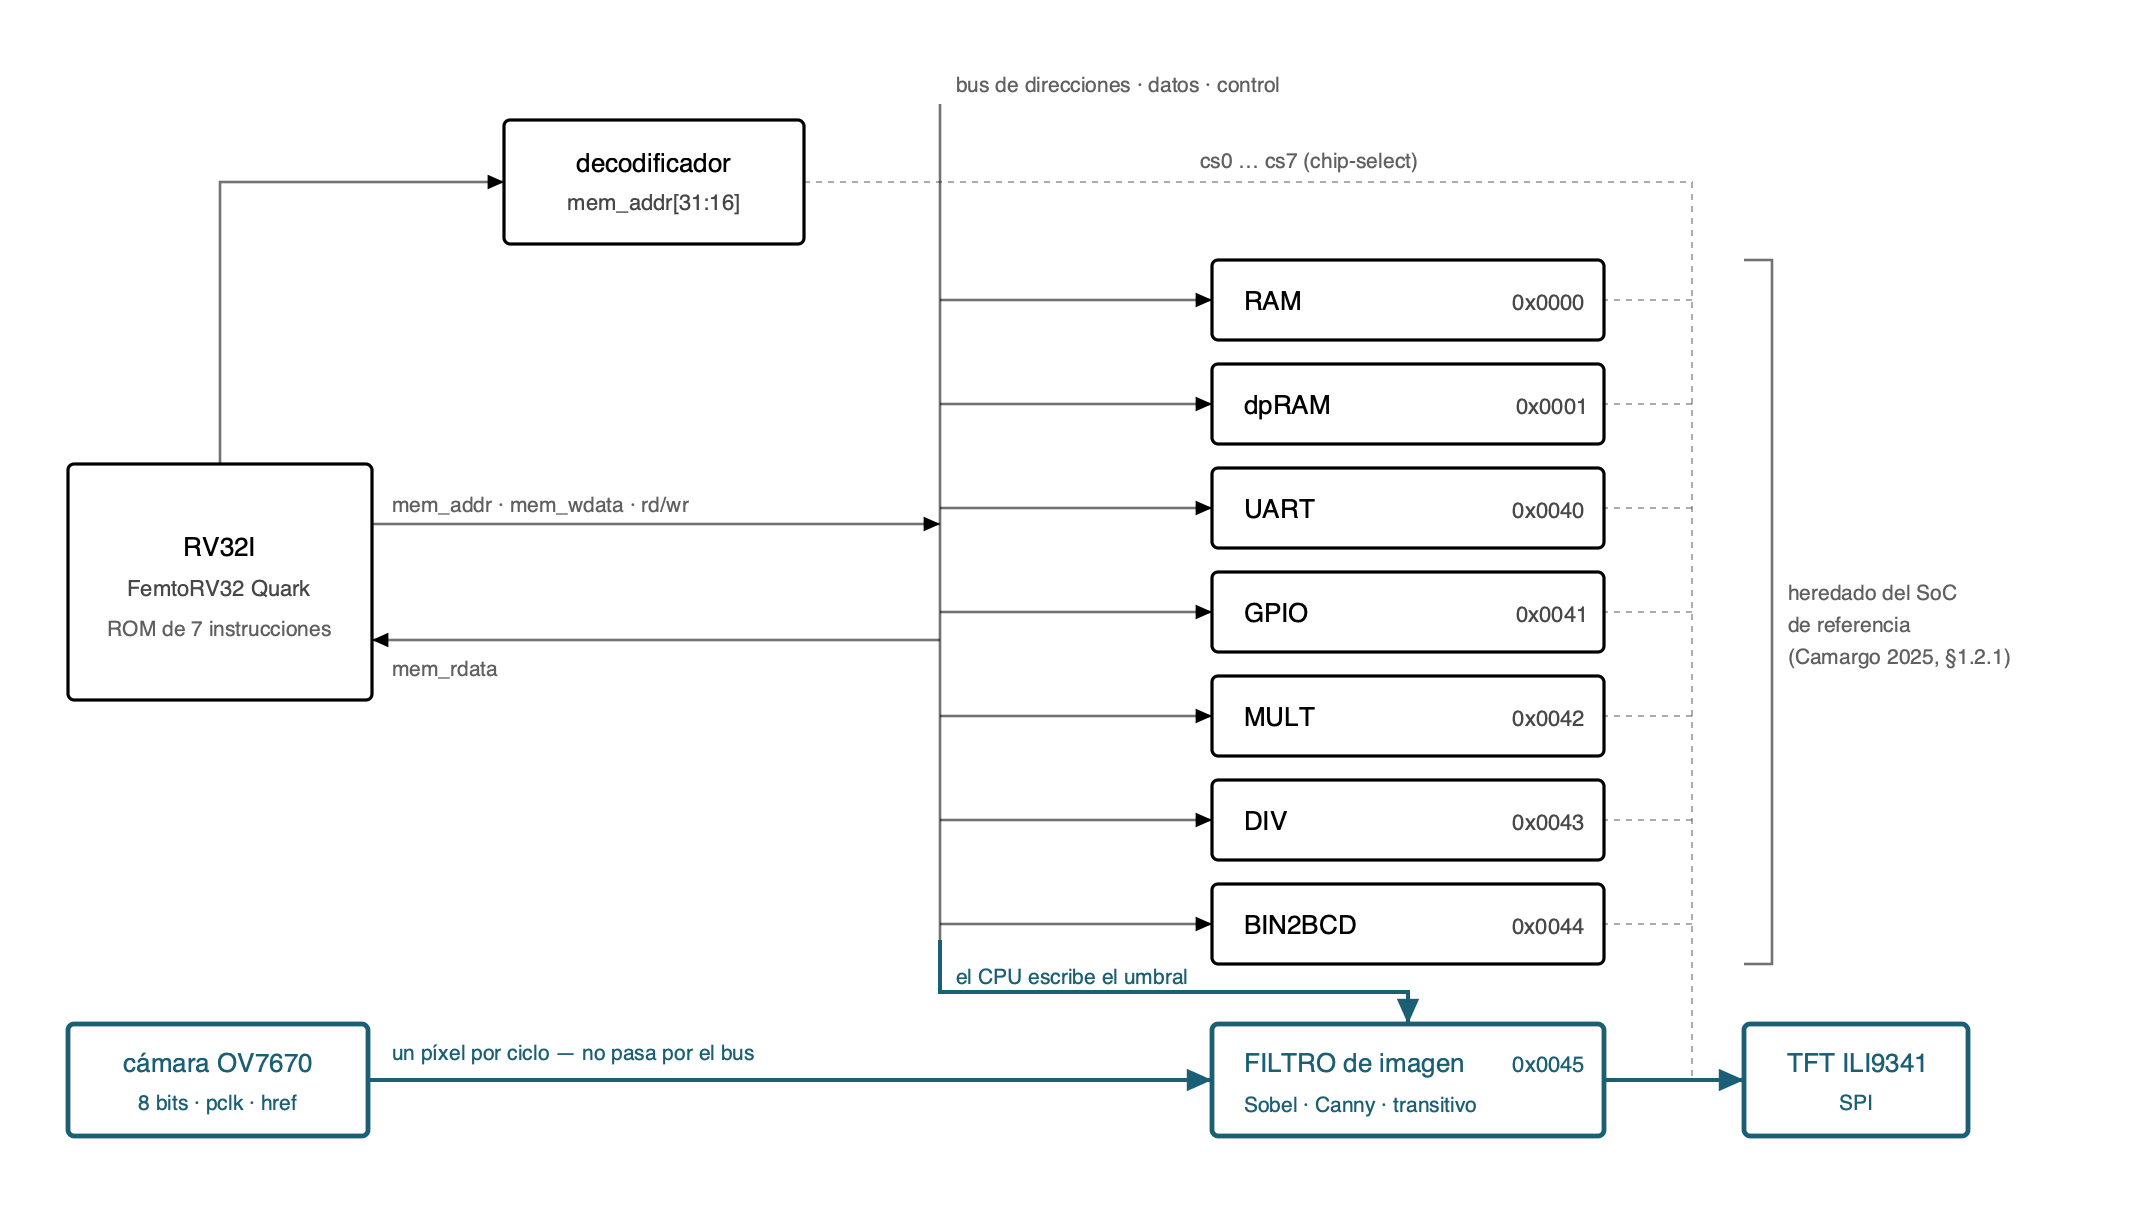
\includegraphics[keepaspectratio,alt={Figura 4.1. El sistema en silicio, en el lenguaje de bloques del SoC de referencia. Los siete periféricos en gris son los heredados; el que aparece destacado, en la base 0x0045, es la aportación de este trabajo. Obsérvese que el camino de datos de imagen no pasa por el bus: los píxeles entran de la cámara al filtro y salen de éste a la pantalla a un píxel por ciclo, y lo único que el procesador pone en el bus es el umbral.}]{figuras/fig_4_1_soc.png}}
\caption{\textbf{Figura 4.1.} El sistema en silicio, en el lenguaje de
bloques del SoC de referencia. Los siete periféricos en gris son los
heredados; el que aparece destacado, en la base \texttt{0x0045}, es la
aportación de este trabajo. Obsérvese que \textbf{el camino de datos de
imagen no pasa por el bus}: los píxeles entran de la cámara al filtro y
salen de éste a la pantalla a un píxel por ciclo, y lo único que el
procesador pone en el bus es el umbral.}
\end{figure}

La figura muestra por qué este periférico no se parece a los demás. Un
multiplicador o un divisor reciben sus operandos por el bus y devuelven
el resultado por el bus: el procesador los usa. El filtro, en cambio,
\textbf{tiene su propio camino de datos} ---de la cámara a la pantalla,
a un píxel por ciclo--- y del bus recibe únicamente un parámetro de
configuración. El procesador no lo usa: lo \textbf{ajusta}.

\begin{quote}
Esa distinción es la que el Capítulo 6 convierte en argumento. Un
periférico que procesa a través del bus está limitado por el ancho de
banda del bus; uno que procesa al margen de él, no. Es la razón de que
un sistema de visión en tiempo real pueda construirse sobre un
procesador de siete instrucciones.
\end{quote}

El firmware ocupa \textbf{siete instrucciones}: inicializa, escribe el
umbral y queda en un lazo. No es un programa modesto por limitación sino
por diseño --- el procesador existe para poder cambiar un parámetro en
tiempo de ejecución, no para procesar.

\subsection{La ROM sintetizada}\label{la-rom-sintetizada}

En una FPGA el contenido de la memoria de programa se carga con el
\emph{bitstream}. \textbf{En un ASIC no hay nada que lo cargue}: los
biestables arrancan en un estado indefinido. La memoria de programa debe
por tanto sintetizarse como lógica combinacional ---una tabla de
constantes--- y no como un arreglo inicializado.

Es el primero de los cuatro cambios obligatorios de la §4.8, y el que
más sorprende a quien llega desde FPGA, porque el código funciona
idénticamente en simulación en ambos casos.

\section{4.6 Memoria: la batalla de los
recursos}\label{memoria-la-batalla-de-los-recursos}

La iCE40UP5K ofrece tres clases de almacenamiento, y el diseño usa las
tres con criterios distintos:

\begin{longtable}[]{@{}
  >{\raggedright\arraybackslash}p{(\linewidth - 4\tabcolsep) * \real{0.3333}}
  >{\raggedright\arraybackslash}p{(\linewidth - 4\tabcolsep) * \real{0.3333}}
  >{\raggedright\arraybackslash}p{(\linewidth - 4\tabcolsep) * \real{0.3333}}@{}}
\toprule\noalign{}
\begin{minipage}[b]{\linewidth}\raggedright
Recurso
\end{minipage} & \begin{minipage}[b]{\linewidth}\raggedright
Cantidad
\end{minipage} & \begin{minipage}[b]{\linewidth}\raggedright
Uso en este trabajo
\end{minipage} \\
\midrule\noalign{}
\endhead
\bottomrule\noalign{}
\endlastfoot
Celdas lógicas & 5 280 & lógica y registros pequeños \\
Bloques de memoria (4 kbit) & 30 & \textbf{memorias de línea} de las
ventanas 3×3 \\
SPRAM (256 kbit) & 4 & \textbf{framebuffers} del filtro transitivo \\
\end{longtable}

La asignación no es libre: una memoria de línea cabe en un bloque de
memoria si el sintetizador la reconoce como tal, y no la reconoce si el
código la escribe de una forma que no encaja con el patrón esperado.
Varios de los problemas de recursos del desarrollo fueron de esa
naturaleza ---memorias que se convertían en biestables por un detalle de
escritura del RTL--- y no de tamaño real del diseño.

El caso más costoso fue un \textbf{ancho de puntero insuficiente}: un
contador de direcciones con un bit de menos del necesario direcciona la
mitad de la memoria y sobrescribe la otra, produciendo una imagen que se
ve plausible pero está mal. Como en el caso del byte de luminancia, el
error sobrevive a la inspección visual.

\begin{quote}
Este apartado es el origen del título del Capítulo 6. En la FPGA los dos
primeros recursos parecen gratuitos porque ya están en el sustrato; en
el ASIC ninguno lo es, y el mismo RTL que allí cabía holgadamente aquí
define el tamaño del dado.
\end{quote}

\section{4.7 Del RTL a la FPGA}\label{del-rtl-a-la-fpga}

El camino a la FPGA impuso sus propias decisiones.

\textbf{El intercambio entre celdas lógicas y bloques de memoria.}
Forzar más memorias de línea a bloques libera celdas pero consume
bloques, que son treinta. En varios puntos del desarrollo el diseño
estuvo limitado alternativamente por uno y por otro, y la solución
consistió en mover recursos entre ambos hasta encontrar una combinación
que cerrara.

\textbf{El bug del cerrojo.} Una asignación condicional incompleta
dentro de un bloque combinacional infiere un cerrojo en lugar de lógica.
El diseño sintetiza, ocupa recursos parecidos y funciona en simulación;
en la placa produce un comportamiento dependiente de la temporización.
La herramienta lo advierte, y la advertencia es fácil de ignorar entre
otras muchas.

\textbf{El bring-up incremental.} El sistema se puso en marcha por
etapas, cada una verificable por sí misma: parpadeo, reloj,
configuración SCCB, imagen en gris, memorias de línea, filtro, umbral,
motor, procesador. La razón es que \textbf{cada etapa es el banco de
pruebas de la siguiente}: cuando el filtro no produjo imagen, disponer
de la etapa anterior funcionando permitió decidir en un solo intento si
el problema estaba en el filtro o en la captura.

\section{4.8 Del RTL al ASIC: los cuatro cambios
obligatorios}\label{del-rtl-al-asic-los-cuatro-cambios-obligatorios}

El mismo Verilog no sirve para los dos destinos. Cuatro cosas hay que
cambiar, y ninguna de ellas produce un error de simulación ---por eso
son peligrosas.

\textbf{1. La memoria de programa debe sintetizarse.} Ya explicado en la
§4.5: en silicio no existe el \emph{bitstream} que la inicializa.

\textbf{2. Reset explícito en todos los registros de control.} En una
FPGA los biestables arrancan en el valor que el \emph{bitstream} les da;
en silicio arrancan en un estado indefinido. Toda máquina de estados
necesita una señal de reinicio explícita, y omitirla produce un circuito
que en simulación arranca correctamente y en la mesa no arranca nunca.

\textbf{3. Fuera el tri-estado interno.} El bus de datos de la cámara es
bidireccional y en FPGA se describe con alta impedancia dentro del
diseño. Un ASIC de celda estándar no dispone de eso: la señal debe
partirse en un dato y un habilitador ---\texttt{cam\_sda\_o} y
\texttt{cam\_sda\_oe}--- y el tri-estado real ocurre en el anillo de
pads.

\textbf{4. Fuera las primitivas del fabricante.} Los bloques específicos
de Lattice ---el controlador del LED RGB, entre otros--- no existen en
sky130. Se sustituyen por pines ordinarios o se eliminan.

\begin{quote}
Los cuatro cambios comparten una propiedad que conviene subrayar:
\textbf{ninguno produce un fallo visible en simulación RTL}. Un diseño
con \texttt{initial} heredado de FPGA simula perfectamente y sale de
fábrica mudo. Los dos únicos que se detectaron a tiempo durante este
trabajo aparecieron en \textbf{simulación de compuertas}, después de la
síntesis, y no antes.
\end{quote}

\chapter{5. Resultados}\label{resultados}

\section{5.1 Verificación funcional}\label{verificaciuxf3n-funcional}

\begin{quote}
\textbf{Estado:} borrador 1, escrito el 2026-09-16. Fuente: cuaderno 1,
Partes 29-35. Formato Markdown para convertir con \texttt{pandoc} a Word
o LaTeX según decida la guía de la Facultad.
\end{quote}

Antes de presentar área, frecuencia o consumo conviene establecer que
los circuitos \textbf{calculan lo que deben calcular}. Esta sección lo
hace, y distingue con cuidado dos preguntas que la literatura de
implementación mezcla con frecuencia: si el hardware coincide con su
modelo de referencia, y si el resultado es bueno. Aquí sólo se responde
la primera. La segunda pertenece a la §5.6.

\subsection{5.1.1 El criterio}\label{el-criterio}

Cada filtro se especificó primero como un programa en Python ---el
\textbf{modelo golden} descrito en la §3.2--- y sólo después se escribió
su descripción en Verilog. La verificación consiste en ejecutar ambos
sobre la misma entrada y comparar \textbf{píxel a píxel}, no en
inspeccionar visualmente la salida.

La distinción no es formal. Un mapa de bordes erróneo sigue pareciendo
un mapa de bordes, de modo que la inspección visual no distingue un
circuito correcto de uno que desplaza una fila, satura un byte o
invierte un signo. Sólo la comparación numérica lo hace.

Al comparar se admite un \textbf{desplazamiento constante} entre ambas
salidas ---la técnica de \emph{best-shift} de la §3.3--- porque la
implementación en hardware introduce una latencia de segmentación que el
modelo en software no tiene. Un desfase uniforme de \emph{k} píxeles no
es un error de cálculo sino una propiedad de la arquitectura segmentada,
y se descuenta explícitamente; cualquier diferencia que sobreviva a esa
corrección sí lo es.

\subsection{5.1.2 Resultado sobre los núcleos
aislados}\label{resultado-sobre-los-nuxfacleos-aislados}

Los tres núcleos son \textbf{idénticos bit a bit} a su modelo de
referencia. En el caso del Sobel sobre un cuadro de 60×80, la
comparación arroja \textbf{0 píxeles de diferencia sobre 4 800}, y el
resultado se sostiene para los tres filtros sobre las cinco imágenes de
prueba.

\begin{longtable}[]{@{}lrrr@{}}
\toprule\noalign{}
Núcleo & Imágenes & Píxeles comparados & Diferencias \\
\midrule\noalign{}
\endhead
\bottomrule\noalign{}
\endlastfoot
Sobel 3×3 & 5 / 5 & 4 800 por cuadro & \textbf{0} \\
Canny de un salto & 5 / 5 & 4 800 por cuadro & \textbf{0} \\
Canny transitivo & 5 / 5 & 4 800 por cuadro & \textbf{0} \\
\end{longtable}

Que la coincidencia sea exacta y no aproximada tiene una causa de
diseño: los tres filtros operan \textbf{sobre enteros y sin división}.
La magnitud del gradiente usa la norma L1,
\texttt{\textbar{}Gx\textbar{}+\textbar{}Gy\textbar{}}, en lugar de la
euclídea; los pesos del operador son potencias de dos, implementadas
como desplazamientos; y el umbral es una comparación. No hay ninguna
operación cuyo redondeo pueda diferir entre una biblioteca de punto
flotante y un circuito. \textbf{La igualdad bit a bit no es una
casualidad afortunada: es consecuencia de haber elegido una aritmética
que la permite.}

\subsection{5.1.3 Resultado sobre la cadena completa con
cámara}\label{resultado-sobre-la-cadena-completa-con-cuxe1mara}

La verificación anterior alimenta el circuito con una imagen almacenada.
La cadena real recibe en cambio un flujo de video de la cámara OV7670,
con sus bordes de línea, sus tiempos muertos y su sincronismo propio.
Medida sobre ese flujo, la concordancia entre el hardware y el modelo
es:

\begin{longtable}[]{@{}lr@{}}
\toprule\noalign{}
Cadena & Concordancia \\
\midrule\noalign{}
\endhead
\bottomrule\noalign{}
\endlastfoot
Sobel & 95 -- 100 \% \\
Canny de un salto & 88 -- 99 \% \\
Canny transitivo & 96 -- 100 \% \\
Promedio a través del SoC & \textbf{97,8 \%} \\
\end{longtable}

La degradación respecto del 100 \% de la §5.1.2 no proviene del filtro
sino del \textbf{acoplamiento con la cámara}: el muestreo del flujo, el
recorte de la ventana y el instante exacto en que empieza un cuadro
introducen diferencias de uno o dos píxeles en los bordes de la imagen.
El valor más bajo corresponde al Canny de un salto, que es también el
más sensible por construcción ---un píxel que cruza el umbral alto
propaga su decisión a sus vecinos, de modo que una diferencia aislada en
la entrada puede producir varias en la salida.

\begin{quote}
\textbf{Dos precisiones de terminología, porque el número se presta a
confusión.}

Primera: los porcentajes de esta tabla son \textbf{concordancia entre el
hardware y su propio modelo de referencia}, no exactitud del filtro.
Miden si el circuito hace lo que el programa hace, no si lo que el
programa hace es correcto o útil. Un filtro mal diseñado puede alcanzar
el 100 \% de concordancia con un modelo igualmente mal diseñado.

Segunda: la \textbf{densidad de bordes} ---la fracción de píxeles
marcados, en torno al 2 \% en las imágenes de prueba--- aparece en
varias figuras de este trabajo y \textbf{no es una medida de calidad}.
Es una propiedad de la escena y del punto de operación elegido, y su
valor «correcto» depende de para qué se vaya a usar el mapa de bordes.
La §5.6.4 muestra precisamente que mover ese punto de operación cambia
el resultado de clasificación más que cambiar de filtro.
\end{quote}

\section{5.2 Resultados en FPGA}\label{resultados-en-fpga}

\begin{quote}
\textbf{Estado:} borrador 2, 2026-09-21. Fuente: cuaderno 1, Partes
25-28 y 68-82, y los informes de \texttt{nextpnr-ice40} conservados de
las corridas del 30 de julio y del 3 de agosto de 2026.
\end{quote}

Los resultados de esta sección son de una clase distinta a los del resto
del capítulo: no provienen de un informe de herramienta sino de
\textbf{un circuito que funciona sobre una mesa}, con una cámara
apuntando a un objeto y una pantalla mostrando el resultado. Es la única
parte del trabajo donde el sistema completo existe físicamente, y por
eso condiciona lo que puede afirmarse de las demás.

\subsection{5.2.1 La plataforma}\label{la-plataforma}

La implementación física se realizó sobre una \textbf{iCE40UP5K} en
tarjeta iCESugar v1.5, con una cámara \textbf{OV7670} y una pantalla
\textbf{TFT ILI9341} por SPI. El flujo de síntesis e implementación es
enteramente abierto: \texttt{yosys} para síntesis,
\texttt{nextpnr-ice40} para emplazamiento y ruteo, \texttt{icepack} para
el \emph{bitstream}.

La elección del dispositivo no es incidental. La iCE40UP5K ofrece 5 280
celdas lógicas, 30 bloques de memoria de 4 kbit y \textbf{cuatro bloques
de SPRAM de 256 kbit} --- y son estos últimos los que hacen posible el
filtro transitivo, porque permiten alojar el cuadro completo sin
consumir lógica. Esa disponibilidad es exactamente lo que desaparece al
pasar a un ASIC sin macro de memoria, y es el origen del resultado de la
§5.4.3.

\subsection{5.2.2 Los tres filtros,
funcionando}\label{los-tres-filtros-funcionando}

\begin{longtable}[]{@{}
  >{\raggedright\arraybackslash}p{(\linewidth - 6\tabcolsep) * \real{0.2500}}
  >{\raggedright\arraybackslash}p{(\linewidth - 6\tabcolsep) * \real{0.2500}}
  >{\raggedright\arraybackslash}p{(\linewidth - 6\tabcolsep) * \real{0.2500}}
  >{\raggedright\arraybackslash}p{(\linewidth - 6\tabcolsep) * \real{0.2500}}@{}}
\toprule\noalign{}
\begin{minipage}[b]{\linewidth}\raggedright
Filtro
\end{minipage} & \begin{minipage}[b]{\linewidth}\raggedright
Arquitectura
\end{minipage} & \begin{minipage}[b]{\linewidth}\raggedright
Implementación física
\end{minipage} & \begin{minipage}[b]{\linewidth}\raggedright
Umbrales en la placa
\end{minipage} \\
\midrule\noalign{}
\endhead
\bottomrule\noalign{}
\endlastfoot
Sobel & flujo & hardware, con procesador FemtoRV32 & 90 \\
Canny de un salto & flujo & hardware, con procesador FemtoRV32 & 50 /
20 \\
Canny transitivo & \textbf{framebuffer} & hardware, motor en Verilog
\textbf{sin procesador} & 60 / 30 \\
\end{longtable}

Los tres funcionan sobre la placa con cámara y pantalla en vivo. El
transitivo produce contornos \textbf{conectados y completos} ---una
letra cerrada aparece cerrada--- frente a los bordes locales de los
otros dos, que es precisamente lo que su punto fijo debe conseguir.

\begin{figure}
\centering
\pandocbounded{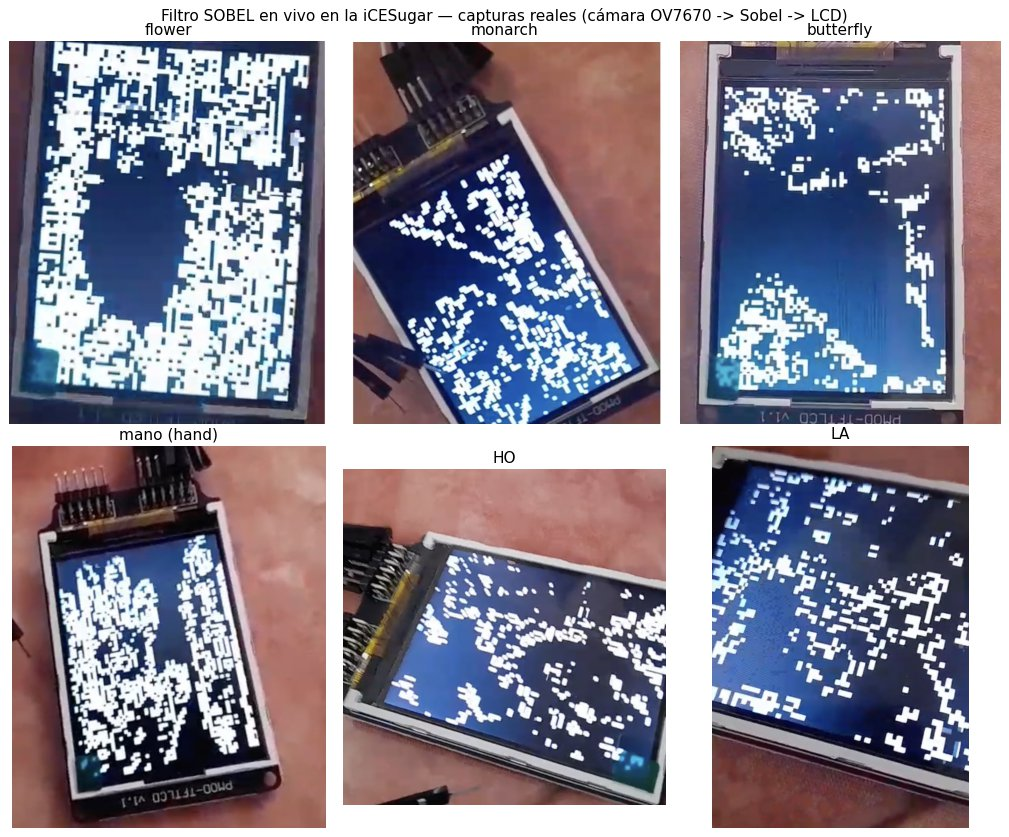
\includegraphics[keepaspectratio,alt={Figura 5.1. El filtro Sobel corriendo en vivo sobre la iCESugar, fotografiado directamente de la pantalla. Seis escenas distintas ---una flor, dos mariposas, una mano y dos letras--- recorren la cadena completa cámara → filtro → pantalla sin intervención de ningún computador. Son capturas del montaje físico, no reconstrucciones: la propia tarjeta y el cableado del módulo aparecen en el encuadre.}]{figuras/fig_5_1_sobel_en_vivo.jpg}}
\caption{\textbf{Figura 5.1.} El filtro Sobel corriendo en vivo sobre la
iCESugar, fotografiado directamente de la pantalla. Seis escenas
distintas ---una flor, dos mariposas, una mano y dos letras--- recorren
la cadena completa cámara → filtro → pantalla sin intervención de ningún
computador. Son capturas del montaje físico, no reconstrucciones: la
propia tarjeta y el cableado del módulo aparecen en el encuadre.}
\end{figure}

\subsection{5.2.3 Utilización del
dispositivo}\label{utilizaciuxf3n-del-dispositivo}

La tabla recoge el \textbf{Device utilisation} que informa
\texttt{nextpnr-ice40} tras el emplazamiento y ruteado
---\texttt{-\/-up5k\ -\/-package\ sg48}---, que es la medida
autoritativa: la que dice si el diseño entra en el dispositivo. Las
cinco filas de una misma columna proceden de \textbf{una sola corrida
con una sola versión de las herramientas}, para que sean comparables
entre sí.

\begin{longtable}[]{@{}
  >{\raggedright\arraybackslash}p{(\linewidth - 12\tabcolsep) * \real{0.1111}}
  >{\raggedleft\arraybackslash}p{(\linewidth - 12\tabcolsep) * \real{0.1481}}
  >{\raggedleft\arraybackslash}p{(\linewidth - 12\tabcolsep) * \real{0.1481}}
  >{\raggedleft\arraybackslash}p{(\linewidth - 12\tabcolsep) * \real{0.1481}}
  >{\raggedleft\arraybackslash}p{(\linewidth - 12\tabcolsep) * \real{0.1481}}
  >{\raggedleft\arraybackslash}p{(\linewidth - 12\tabcolsep) * \real{0.1481}}
  >{\raggedleft\arraybackslash}p{(\linewidth - 12\tabcolsep) * \real{0.1481}}@{}}
\toprule\noalign{}
\begin{minipage}[b]{\linewidth}\raggedright
Diseño
\end{minipage} & \begin{minipage}[b]{\linewidth}\raggedleft
LC / 5 280
\end{minipage} & \begin{minipage}[b]{\linewidth}\raggedleft
BRAM / 30
\end{minipage} & \begin{minipage}[b]{\linewidth}\raggedleft
SPRAM / 4
\end{minipage} & \begin{minipage}[b]{\linewidth}\raggedleft
E/S / 39
\end{minipage} & \begin{minipage}[b]{\linewidth}\raggedleft
\emph{f}máx sistema
\end{minipage} & \begin{minipage}[b]{\linewidth}\raggedleft
\emph{f}máx cámara
\end{minipage} \\
\midrule\noalign{}
\endhead
\bottomrule\noalign{}
\endlastfoot
Transitivo, motor dedicado \textbf{sin procesador} & 2 426 (45 \%) & 17
(56 \%) & \textbf{2 (50 \%)} & 18 (46 \%) & \textbf{28,7 MHz} ✓ & 20,6
MHz ✓ \\
SoC + Sobel & 4 848 (91 \%) & 20 (66 \%) & 0 & 18 (46 \%) & 9,5 MHz ✗ &
20,7 MHz ✓ \\
SoC + Canny de un salto & 5 234 (\textbf{99 \%}) & 24 (80 \%) & 0 & 18
(46 \%) & 9,5 MHz ✗ & 17,7 MHz ✓ \\
SoC + transitivo \textbf{por software} & 5 251 (\textbf{99 \%}) & 28 (93
\%) & 0 & 18 (46 \%) & 8,7 MHz ✗ & 20,5 MHz ✓ \\
SoC + transitivo \textbf{como periférico} & no emplaza (≈ 127 \%) & ---
& --- & --- & --- & --- \\
\end{longtable}

\begin{quote}
\textbf{Procedencia.} Las cuatro primeras filas se midieron de nuevo
para este documento. Tres de ellas ---las filas primera, tercera y
cuarta--- reprodujeron \textbf{exactamente}, celda por celda y bloque
por bloque, los informes conservados de las corridas originales de julio
y agosto de 2026. La del SoC + Sobel, cuyo informe de emplazamiento no
se había conservado, arrojó 4 848 celdas frente a las 4 878 anotadas
entonces en el cuaderno; la diferencia, de treinta celdas sobre cinco
mil, proviene de una versión distinta del sintetizador, que produce doce
tablas de consulta menos. La quinta fila no dispone de informe: el
emplazamiento no llegó a completarse, y el ≈ 127 \% es el valor
documentado en su momento.
\end{quote}

De la tabla se desprenden tres lecturas.

\textbf{La memoria grande sólo la usa un diseño.} Los cuatro bloques de
SPRAM ---256 kbit cada uno--- están sin tocar en todas las variantes de
flujo, y sólo el transitivo consume dos. Es coherente con su
arquitectura: es el único que necesita el cuadro entero a la vez. Los
filtros de flujo se las arreglan con dos filas de retardo, que caben en
los bloques de memoria pequeños.

\textbf{El límite de frecuencia lo pone el procesador, y no la
ocupación.} Los tres diseños que llevan el FemtoRV32 se agrupan entre
8,7 y 9,5 MHz mientras que el que no lo lleva alcanza 28,7 MHz:
\textbf{tres veces más rápido}. La tentación es atribuirlo a la
congestión ---los dos más lentos están al 99 \%---, pero la tabla lo
desmiente: el SoC del Sobel, \textbf{ocho puntos más vacío} que el del
Canny, cierra a la misma frecuencia, y de hecho una centésima por
debajo. La causa está en el informe de caminos críticos, que en los tres
SoC señala el mismo origen: \textbf{el registro de instrucción del
procesador}. El camino va de un flanco de subida a uno de bajada, de
modo que dispone de \textbf{medio período} en lugar de uno entero, y eso
divide por dos la frecuencia alcanzable. La síntesis lo confirma por
otra vía: los tres SoC contienen \textbf{2 048 biestables sensibles al
flanco de bajada} y el diseño sin procesador no contiene
\textbf{ninguno}. No es un problema de emplazamiento sino una propiedad
del procesador elegido, y es la razón de fondo de que las tres variantes
con CPU necesiten dividir el reloj.

\textbf{El sensor nunca fue el límite.} El dominio de la cámara cierra
con holgura en las cuatro filas medidas ---entre 17,7 y 20,7 MHz frente
a los 12 necesarios---, y es el del sistema el que falla. El cuello de
botella está del lado del procesamiento, no de la adquisición.

\begin{quote}
\textbf{Y una observación sobre el sustrato.} En los cuatro diseños el
retardo del camino crítico está dominado por el \textbf{ruteado}, que
aporta entre el 62 \% y el 72 \% del total; la lógica aporta el resto.
En una malla de interconexión fija como la de una FPGA esto es lo
esperable, y conviene tenerlo presente al leer la §5.4: en el ASIC,
donde el trazado se genera para el diseño concreto, ese reparto es otro.
\end{quote}

\subsection{5.2.4 El hallazgo de
co-diseño}\label{el-hallazgo-de-co-diseuxf1o}

El dato más importante de esta sección no es una cifra de utilización
sino una \textbf{decisión de arquitectura que la medida forzó}.

La intención inicial era que el procesador calculara la histéresis
transitiva por software, como hace en las versiones de los otros dos
filtros. Esa versión existe y funciona en simulación, con un 92,8 \% de
concordancia. Pero al intentar sintetizar el conjunto ---procesador,
memoria, framebuffers y motor--- la ocupación de celdas lógicas alcanzó
el \textbf{127 \%}: no cabía.

La respuesta fue mover el motor de histéresis de software a hardware,
como camino de datos en Verilog sin intervención del procesador. Así
implementado, la síntesis reporta \textbf{1 728 tablas de consulta} y el
emplazamiento \textbf{2 426 celdas lógicas, el 45 \% del dispositivo},
cerrando el temporizado a \textbf{28,7 MHz} con holgura.

\begin{quote}
Las dos cifras anteriores no son la misma medida, y conviene no
confundirlas: la celda lógica de la iCE40 empaqueta una tabla de
consulta \textbf{y} un biestable, de modo que un diseño con muchos
biestables sueltos ocupa más celdas que tablas tiene. Dividir el
recuento de tablas entre las 5 280 celdas del dispositivo da un 33 \%
que \textbf{subestima la ocupación real en doce puntos}. La cifra válida
es la del emplazamiento, no la de la síntesis; esta sección usa sólo la
primera.
\end{quote}

\begin{quote}
\textbf{Por qué esto es co-diseño y no una optimización.} No se trata de
que el hardware sea más rápido que el software, que es lo esperable. Se
trata de que \textbf{la restricción de recursos cambió el reparto de
responsabilidades entre las dos mitades del sistema}: la misma función,
expresada como programa, no cabía; expresada como circuito, ocupa un
tercio del dispositivo. La frontera entre lo que ejecuta el procesador y
lo que ejecuta la lógica dedicada no la fijó una preferencia de diseño
sino una medición.
\end{quote}

Este resultado reaparece transformado en la §5.4.2: en el ASIC, donde el
área no está acotada por un dispositivo fijo, el procesador vuelve a ser
viable junto al transitivo y cuesta unas nueve mil celdas. La misma
pregunta tiene respuestas opuestas en los dos sustratos.

\subsection{5.2.5 Umbrales de laboratorio y umbrales de
cámara}\label{umbrales-de-laboratorio-y-umbrales-de-cuxe1mara}

Las tres filas de la tabla anterior muestran umbrales distintos de los
que se usan en simulación. El transitivo, por ejemplo, pasó de 110/70 en
el banco de pruebas a \textbf{60/30 en la placa}.

El ajuste no es arbitrario ni es un defecto: una imagen almacenada y un
flujo de cámara tienen histogramas distintos, y el punto de operación
que extrae la estructura de una no es el que la extrae de la otra. La
§5.6.4 mide exactamente cuánto importa esa elección, y muestra que
\textbf{mover el umbral dentro de un filtro cambia el resultado de
clasificación más que cambiar de filtro}.

\begin{center}\rule{0.5\linewidth}{0.5pt}\end{center}

\begin{quote}
\textbf{Sobre la reproducibilidad de estas cifras.} Las cuatro filas
medidas se rehicieron el 21 de septiembre de 2026 con el guion
\texttt{medir\_utilizacion\_vm.sh}, que aplica a cada diseño las mismas
órdenes de lectura de fuentes que su guion de construcción original.
Tres de las cuatro reprodujeron el informe conservado sin desviarse en
una sola celda ni en un solo bloque de memoria, pese a mediar casi dos
meses entre una corrida y otra. La cuarta se desvió en treinta celdas
sobre cinco mil, y la causa está identificada: una versión distinta del
sintetizador. \textbf{El flujo es determinista a herramientas iguales},
que es lo que permite presentar estas cifras como medidas y no como
estimaciones.
\end{quote}

\section{5.3 Resultados en ASIC: los
bloques}\label{resultados-en-asic-los-bloques}

\begin{quote}
\textbf{Estado:} borrador 1, escrito el 2026-09-16. Fuente: cuaderno 1,
Partes 86-131, y el archivo de planos \texttt{ASIC\_planos/}.
\textbf{Recuento homogeneizado el 21 de septiembre de 2026.} Toda la
columna «celdas» de esta tabla son \textbf{celdas lógicas tras
emplazamiento y ruteado}, recontadas con un mismo criterio desde los
netlists archivados. Véase la §5.3.3 para cruzarlas con las de la §5.4.
\end{quote}

Esta sección presenta los circuitos que implementan \textbf{una función
cada uno}: los tres filtros por separado, los mismos con procesador, dos
bloques de interfaz y dos sistemas de visión. Son el vocabulario con el
que se construyen los sistemas de la §5.4, y su valor está en que
permiten atribuir el costo de cada pieza por separado.

Todos se llevaron a GDSII con \textbf{OpenLane} sobre el PDK abierto
\textbf{sky130A}, biblioteca \texttt{sky130\_fd\_sc\_hd}.

\subsection{5.3.1 La tabla}\label{la-tabla}

\begin{longtable}[]{@{}
  >{\raggedright\arraybackslash}p{(\linewidth - 8\tabcolsep) * \real{0.1765}}
  >{\raggedright\arraybackslash}p{(\linewidth - 8\tabcolsep) * \real{0.1765}}
  >{\raggedleft\arraybackslash}p{(\linewidth - 8\tabcolsep) * \real{0.2353}}
  >{\raggedleft\arraybackslash}p{(\linewidth - 8\tabcolsep) * \real{0.2353}}
  >{\centering\arraybackslash}p{(\linewidth - 8\tabcolsep) * \real{0.1765}}@{}}
\toprule\noalign{}
\begin{minipage}[b]{\linewidth}\raggedright
Circuito
\end{minipage} & \begin{minipage}[b]{\linewidth}\raggedright
Función
\end{minipage} & \begin{minipage}[b]{\linewidth}\raggedleft
Área del die
\end{minipage} & \begin{minipage}[b]{\linewidth}\raggedleft
Celdas
\end{minipage} & \begin{minipage}[b]{\linewidth}\centering
Signoff
\end{minipage} \\
\midrule\noalign{}
\endhead
\bottomrule\noalign{}
\endlastfoot
\texttt{sobel} & filtro Sobel 3×3 & 0,167 mm² & 5 823 & DRC/LVS/XOR =
0 \\
\texttt{canny1} & Canny de un salto, en flujo & 0,360 mm² & 12 993 &
DRC/LVS/XOR = 0 \\
\texttt{transitivo} & Canny con histéresis transitiva & 3,13 mm² & 65
659 & DRC/LVS/XOR = 0 \\
\texttt{soc\_sobel} & FemtoRV32 + Sobel & 0,37 mm² & 12 043 &
DRC/LVS/XOR = 0 \\
\texttt{soc\_canny1} & FemtoRV32 + Canny de un salto & 0,67 mm² & 22 054
& DRC/LVS/XOR = 0 \\
\texttt{soc\_trans} & FemtoRV32 + transitivo & 3,42 mm² & 72 337 &
DRC/LVS/XOR = 0 \\
\texttt{cam\_frontend} & front-end de cámara OV7670 & 0,0177 mm² & 562 &
DRC/LVS/XOR = 0 \\
\texttt{lcd\_ili9341} & driver de pantalla TFT por SPI & 0,0174 mm² &
553 & DRC/LVS/XOR = 0 \\
\texttt{vision\_top} & cámara + Sobel + framebuffer + pantalla & 1,75
mm² & 35 653 & DRC/LVS/XOR = 0 \\
\texttt{vision\_canny} & cámara + Canny + framebuffer + pantalla & 2,04
mm² & 41 925 & DRC/LVS/XOR = 0 \\
\end{longtable}

\textbf{Diez circuitos, diez veces DRC, LVS y XOR en cero.}

\subsection{5.3.2 Lo que la tabla muestra de un
vistazo}\label{lo-que-la-tabla-muestra-de-un-vistazo}

\textbf{El filtro transitivo cuesta casi veinte veces más área que el
Sobel} ---3,13 mm² contra 0,167, y once veces más celdas--- pese a
ejecutar aritmética comparable. La razón, ya anticipada, es el cuadro
completo residente: en la FPGA ese cuadro vivía en SPRAM y no consumía
lógica; aquí es un banco de biestables.

\textbf{Los dos bloques de interfaz son casi gratis.} El front-end de
cámara y el driver de pantalla ocupan menos de dieciocho milésimas de
milímetro cuadrado cada uno, alrededor de 560 celdas. Conviene tenerlo
medido porque desmonta una intuición común: el costo de un sistema de
visión embebido no está en hablar con los periféricos, está en lo que se
hace con los datos entre medias.

\begin{figure}
\centering
\pandocbounded{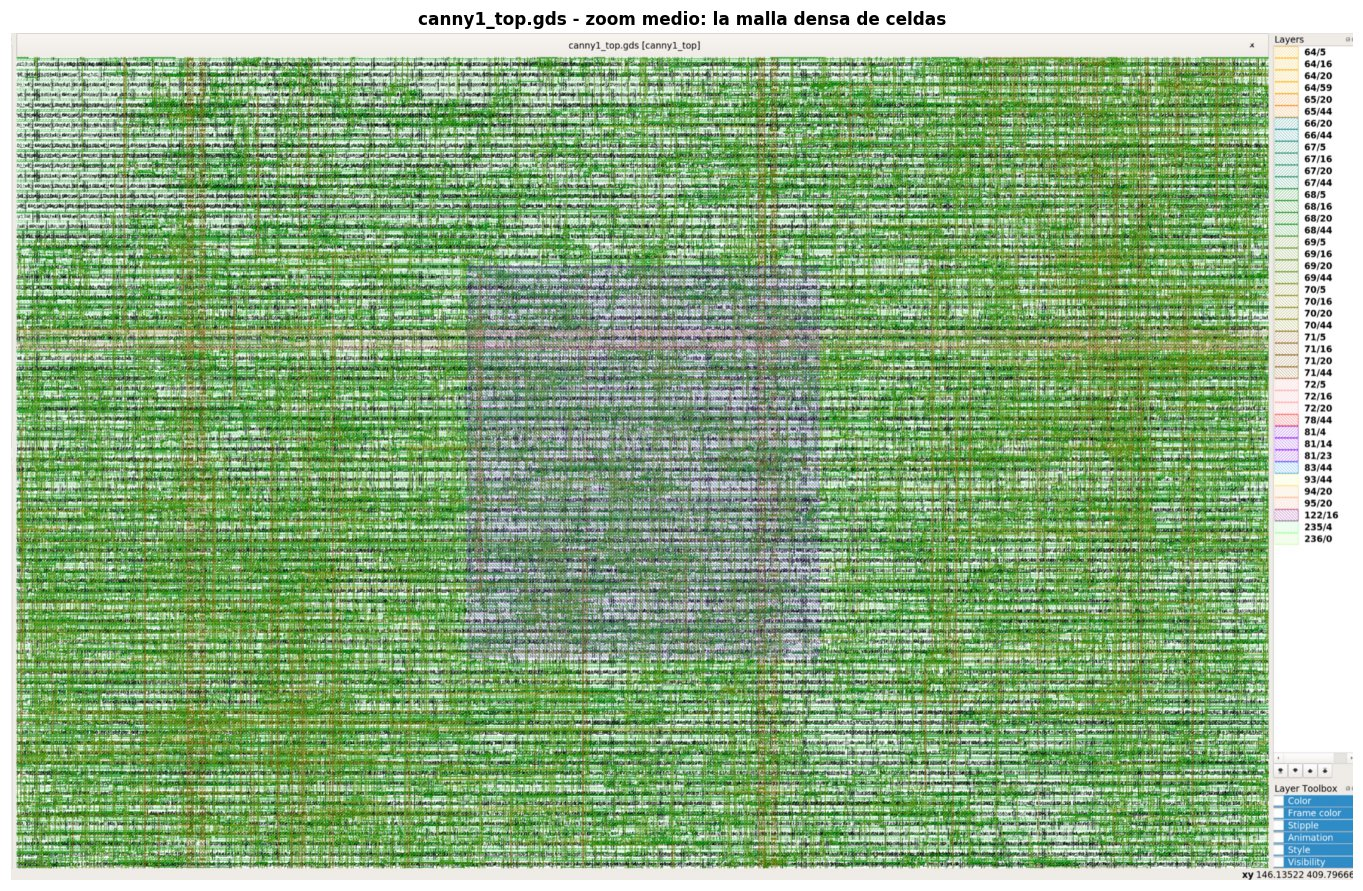
\includegraphics[keepaspectratio,alt={Figura 5.2. Acercamiento al GDSII del canny1 en KLayout. Lo que se ve no es un esquema sino el plano que iría a fábrica: filas de celdas estándar y, sobre ellas, las capas de metal que las conectan. La mancha más clara del centro es una región de menor densidad de ruteo. Las 12 993 celdas de la tabla anterior son, literalmente, estas.}]{figuras/fig_5_2_malla_canny1.jpg}}
\caption{\textbf{Figura 5.2.} Acercamiento al GDSII del \texttt{canny1}
en KLayout. Lo que se ve no es un esquema sino el plano que iría a
fábrica: filas de celdas estándar y, sobre ellas, las capas de metal que
las conectan. La mancha más clara del centro es una región de menor
densidad de ruteo. Las 12 993 celdas de la tabla anterior son,
literalmente, estas.}
\end{figure}

\textbf{Y el Sobel en silicio es mucho más rápido de lo que la FPGA
permitía.} Su camino crítico quedó en \textbf{7,69 ns} frente a un
objetivo de 20 ns, es decir que soportaría unos 130 MHz, mientras que en
la iCE40 cerraba entre 9 y 28 MHz. En silicio la lógica es rápida;
\textbf{lo caro es el área}, y ése es el eje sobre el que gira todo este
capítulo.

\subsection{5.3.3 El recuento de celdas, y cómo cruzar las dos
tablas}\label{el-recuento-de-celdas-y-cuxf3mo-cruzar-las-dos-tablas}

Esta advertencia no es un tecnicismo: afecta a cualquier comparación que
un lector intente hacer entre esta tabla y la de la §5.4.

Un circuito se puede contar en dos momentos del flujo, y las dos cifras
son legítimas:

\begin{longtable}[]{@{}
  >{\raggedright\arraybackslash}p{(\linewidth - 4\tabcolsep) * \real{0.3333}}
  >{\raggedright\arraybackslash}p{(\linewidth - 4\tabcolsep) * \real{0.3333}}
  >{\raggedright\arraybackslash}p{(\linewidth - 4\tabcolsep) * \real{0.3333}}@{}}
\toprule\noalign{}
\begin{minipage}[b]{\linewidth}\raggedright
Definición
\end{minipage} & \begin{minipage}[b]{\linewidth}\raggedright
Qué cuenta
\end{minipage} & \begin{minipage}[b]{\linewidth}\raggedright
Dónde se usa
\end{minipage} \\
\midrule\noalign{}
\endhead
\bottomrule\noalign{}
\endlastfoot
celdas de \textbf{síntesis} & el resultado de traducir el RTL a
compuertas & la tabla de la §5.4 \\
celdas \textbf{emplazadas} & lo que queda tras emplazar y rutear, con
los amortiguadores que el flujo inserta para el árbol de reloj y la
reparación de tiempos & \textbf{esta} tabla y la §5.6 \\
\end{longtable}

Durante la redacción, la columna «celdas» de este capítulo
\textbf{mezclaba las dos}, porque las fichas del cuaderno habían
registrado en cada momento el campo que la herramienta ofrecía.
\textbf{Se rehízo el recuento}: se contaron las instancias de celda
estándar directamente sobre el \textbf{netlist posterior al ruteado} de
cada circuito archivado, descartando las celdas sin función lógica
---relleno, contactos de pozo, desacoplo y diodos de antena---, con un
único criterio para los dieciséis.

El procedimiento se validó antes de aplicarlo: de los dieciséis
circuitos, \textbf{ocho reprodujeron exactamente la cifra que ya
constaba}, hasta la unidad ---los dos bloques de interfaz, los dos SoC,
los dos sistemas de visión y los dos circuitos en IHP---, que son
precisamente aquellos cuya ficha ya provenía del emplazamiento. Los ocho
restantes cambiaron, y ése era el objetivo.

\subsubsection{El factor de conversión,
medido}\label{el-factor-de-conversiuxf3n-medido}

Como en nueve circuitos se conservan las dos cifras, el paso de una a
otra no hay que estimarlo:

\begin{longtable}[]{@{}ll@{}}
\toprule\noalign{}
\endhead
\bottomrule\noalign{}
\endlastfoot
Casos medidos & 9 \\
Factor medio & \textbf{×1,21} \\
Mediana & ×1,20 \\
Rango & ×1,16 a ×1,26 \\
Desviación típica & 0,04 \\
\end{longtable}

\textbf{El emplazamiento agrega entre un 16 \% y un 26 \% de celdas},
con una dispersión estrecha. De modo que una cifra de la §5.4 se lleva a
la escala de ésta multiplicándola por 1,21, y el error de esa conversión
es de unos pocos puntos porcentuales --- no del 20 \% que separaba las
tablas antes de homogeneizarlas.

\begin{quote}
\textbf{Por qué no se convirtió también la §5.4.} Dos de sus seis
circuitos se archivaron sin netlist, de modo que convertir la tabla
habría exigido estimar dos de las seis filas. Se prefirió dejar cada
tabla \textbf{internamente homogénea} ---la §5.4 entera en celdas de
síntesis, ésta entera en celdas emplazadas--- y publicar el factor que
las relaciona, antes que producir una tabla mixta con dos filas
estimadas. Las comparaciones dentro de cada tabla son exactas; las que
cruzan de una a otra pasan por el factor.
\end{quote}

\section{5.4 Resultados en ASIC: la cadena de visión
completa}\label{resultados-en-asic-la-cadena-de-visiuxf3n-completa}

\begin{quote}
\textbf{Estado:} borrador 1, escrito el 2026-09-16. Fuente: cuaderno 1,
Partes 157-165, y la tabla maestra
\texttt{asic/tabla\_maestra/tabla\_6\_chips.py}, que la genera desde los
\texttt{metrics.csv} del flujo.
\end{quote}

La §5.3 presentó bloques: filtros solos, un front-end de cámara, un
driver de pantalla. Ésta presenta \textbf{sistemas}: seis circuitos que
llevan la cadena entera ---captura, filtrado, almacenamiento y
visualización--- en un solo dado. Los seis están organizados como una
matriz de dos variables, el \textbf{filtro} y la \textbf{presencia de
procesador}, de modo que cada comparación entre dos de ellos aísla una
sola causa.

\subsection{5.4.1 La tabla maestra}\label{la-tabla-maestra}

\begin{longtable}[]{@{}
  >{\raggedright\arraybackslash}p{(\linewidth - 20\tabcolsep) * \real{0.0811}}
  >{\raggedright\arraybackslash}p{(\linewidth - 20\tabcolsep) * \real{0.0811}}
  >{\raggedright\arraybackslash}p{(\linewidth - 20\tabcolsep) * \real{0.0811}}
  >{\centering\arraybackslash}p{(\linewidth - 20\tabcolsep) * \real{0.0811}}
  >{\raggedleft\arraybackslash}p{(\linewidth - 20\tabcolsep) * \real{0.1081}}
  >{\raggedleft\arraybackslash}p{(\linewidth - 20\tabcolsep) * \real{0.1081}}
  >{\raggedleft\arraybackslash}p{(\linewidth - 20\tabcolsep) * \real{0.1081}}
  >{\raggedleft\arraybackslash}p{(\linewidth - 20\tabcolsep) * \real{0.1081}}
  >{\centering\arraybackslash}p{(\linewidth - 20\tabcolsep) * \real{0.0811}}
  >{\centering\arraybackslash}p{(\linewidth - 20\tabcolsep) * \real{0.0811}}
  >{\centering\arraybackslash}p{(\linewidth - 20\tabcolsep) * \real{0.0811}}@{}}
\toprule\noalign{}
\begin{minipage}[b]{\linewidth}\raggedright
\#
\end{minipage} & \begin{minipage}[b]{\linewidth}\raggedright
Chip
\end{minipage} & \begin{minipage}[b]{\linewidth}\raggedright
Filtro
\end{minipage} & \begin{minipage}[b]{\linewidth}\centering
CPU
\end{minipage} & \begin{minipage}[b]{\linewidth}\raggedleft
Área (mm²)
\end{minipage} & \begin{minipage}[b]{\linewidth}\raggedleft
Celdas
\end{minipage} & \begin{minipage}[b]{\linewidth}\raggedleft
Reloj de firma
\end{minipage} & \begin{minipage}[b]{\linewidth}\raggedleft
Setup c/parásitos
\end{minipage} & \begin{minipage}[b]{\linewidth}\centering
DRC
\end{minipage} & \begin{minipage}[b]{\linewidth}\centering
LVS
\end{minipage} & \begin{minipage}[b]{\linewidth}\centering
XOR
\end{minipage} \\
\midrule\noalign{}
\endhead
\bottomrule\noalign{}
\endlastfoot
\#1 & \texttt{sobel\_completo} ᵃ & Sobel & --- & 2,45 & 36 730 & 20 ns
(50,0 MHz) & sin dato ᵇ & 0 & 0 & 0 \\
\#2 & \texttt{canny1\_completo} ᵃ & Canny1 & --- & 2,90 & 42 581 & 20 ns
(50,0 MHz) & sin dato ᵇ & 0 & 0 & 0 \\
\#3 & \texttt{trans\_completo} & Transitivo & --- & 9,61 & 137 092 & 20
ns (50,0 MHz) & \textbf{−19,35 ns} & 0 & 0 & 0 \\
\#4 & \texttt{soc\_sobel\_completo} & Sobel & ✓ & 3,03 & 46 019 & 32 ns
(31,2 MHz) & \textbf{+0,00 ns} & 0 & 0 & 0 \\
\#5 & \texttt{soc\_canny1\_completo} & Canny1 & ✓ & 3,44 & 51 037 & 36
ns (27,8 MHz) & \textbf{+0,00 ns} & 0 & 0 & 0 \\
\#6 & \texttt{soc\_trans\_completo} & Transitivo & ✓ & 10,19 & 146 216 &
36 ns (27,8 MHz) & \textbf{−18,23 ns} & 0 & 0 & 0 \\
\end{longtable}

ᵃ Estos dos se archivaron sin el directorio de reportes; sus cifras
provienen de la ficha del cuaderno y no de un \texttt{metrics.csv} del
flujo. Se marcan porque en una tabla de resultados debe poder decirse de
dónde sale cada número.

ᵇ Su ficha registra el \textbf{WNS nominal} ---0,00 ns, sin
violaciones--- pero no quedó registrado el setup ya con parásitos
extraídos, que es justamente la columna que hunde a los dos transitivos.
Se deja en blanco antes que suponer que cierran.

\textbf{Los seis llegaron a GDSII con DRC, LVS y XOR en cero.} Cuatro
cierran temporizado o carecen del dato para afirmar lo contrario; los
dos transitivos no cierran, y conviene decirlo con el número: el \#3
pediría 39,4 ns ---25,4 MHz--- y el \#6, 54,2 ns, es decir 18,4 MHz en
lugar de los 27,8 solicitados.

\begin{quote}
\textbf{Sobre el recuento de celdas, y es importante al leer junto a la
§5.3.} Las cifras de esta tabla son \textbf{celdas de síntesis}; las de
la §5.3 y la §5.6 son \textbf{celdas emplazadas}. Cada tabla es
internamente homogénea, y el paso de una escala a otra \textbf{está
medido sobre nueve circuitos que conservan las dos cifras}: el
emplazamiento agrega entre un 16 \% y un 26 \%, con un factor medio de
\textbf{×1,21} y una desviación típica de 0,04. Para comparar una cifra
de aquí con una de allá, multiplíquese por 1,21; el detalle del
procedimiento está en la §5.3.3.

Dos de los seis circuitos de esta tabla se archivaron sin
\emph{netlist}, razón por la cual no se convirtió la tabla entera: se
prefirió una tabla homogénea en su propia escala antes que una tabla
mixta con dos filas estimadas.
\end{quote}

\begin{figure}
\centering
\pandocbounded{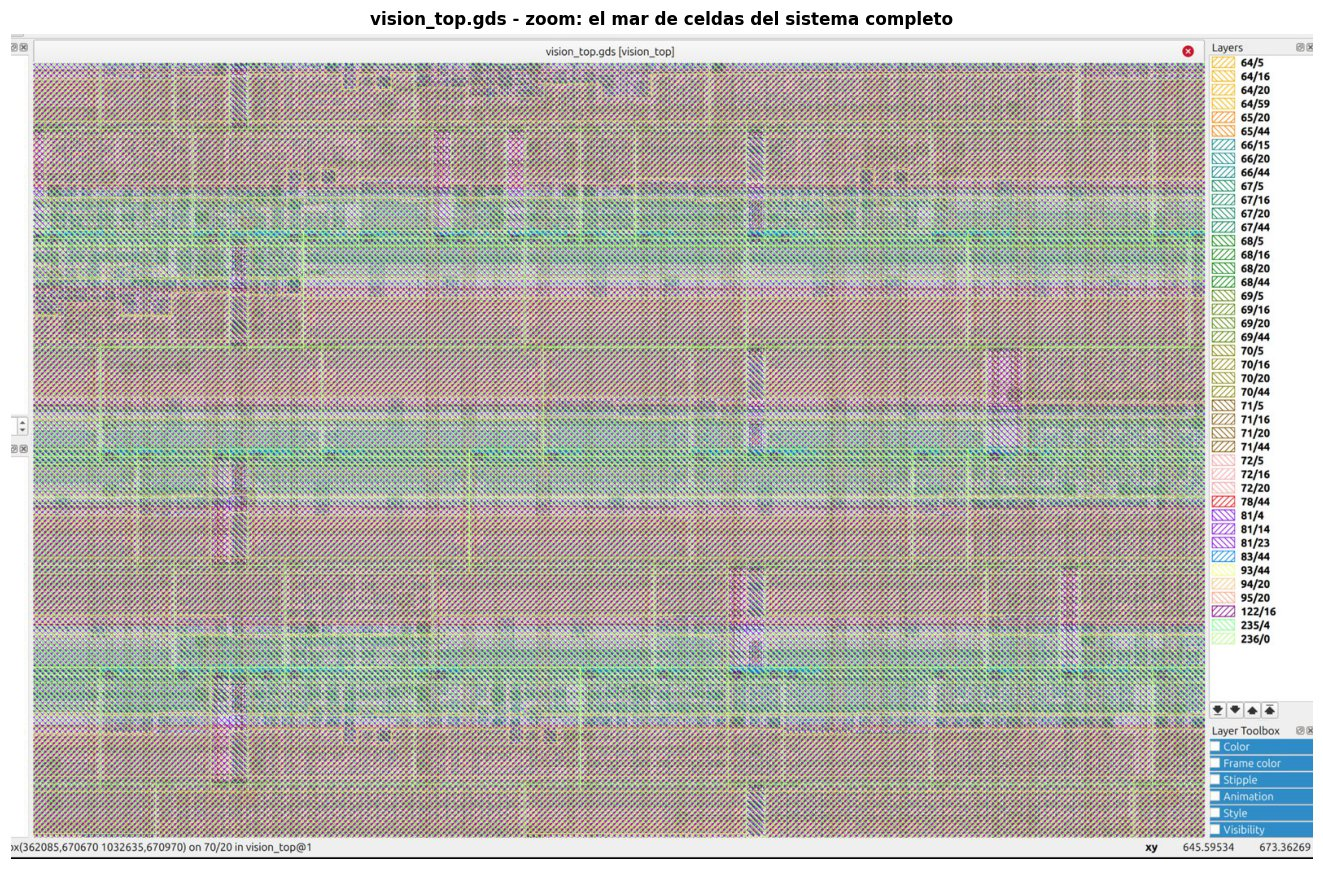
\includegraphics[keepaspectratio,alt={Figura 5.3. El mismo tipo de acercamiento, ahora sobre el sistema de visión completo. La diferencia con la figura anterior no está en la textura sino en la escala: aquí caben cámara, filtro, memoria de cuadro y controlador de pantalla en el mismo dado. Es la forma que toma en silicio la frase «el filtro es una pieza y no el circuito».}]{figuras/fig_5_3_mar_de_celdas_vision.jpg}}
\caption{\textbf{Figura 5.3.} El mismo tipo de acercamiento, ahora sobre
el sistema de visión completo. La diferencia con la figura anterior no
está en la textura sino en la escala: aquí caben cámara, filtro, memoria
de cuadro y controlador de pantalla en el mismo dado. Es la forma que
toma en silicio la frase «el filtro es una pieza y no el circuito».}
\end{figure}

\subsection{5.4.2 El procesador cuesta lo mismo, sea cual sea el
filtro}\label{el-procesador-cuesta-lo-mismo-sea-cual-sea-el-filtro}

Restando cada chip de su gemelo con procesador se obtiene el costo del
FemtoRV32, su memoria de programa y su periférico:

\begin{longtable}[]{@{}lrrrr@{}}
\toprule\noalign{}
Filtro & sin CPU & con CPU & Δ celdas & Δ relativo \\
\midrule\noalign{}
\endhead
\bottomrule\noalign{}
\endlastfoot
Sobel & 36 730 & 46 019 & \textbf{+9 289} & +25,3 \% \\
Canny de un salto & 42 581 & 51 037 & \textbf{+8 456} & +19,9 \% \\
Canny transitivo & 137 092 & 146 216 & \textbf{+9 124} & +6,7 \% \\
\end{longtable}

El incremento absoluto es \textbf{prácticamente constante}: alrededor de
nueve mil celdas, con una dispersión inferior al 5 \% entre el caso más
barato y el más caro. Es un resultado esperable ---el procesador no sabe
qué filtro tiene al lado--- pero conviene tenerlo medido, porque
convierte al procesador en un \textbf{costo fijo y presupuestable}
frente a un datapath cuyo costo varía en un factor de cuatro.

La columna relativa dice lo contrario que la absoluta, y las dos son
ciertas: el mismo procesador representa una cuarta parte del chip más
pequeño y apenas una quinceava parte del más grande. Cuál de las dos
lecturas importa depende de la pregunta. Para decidir si añadir un
procesador a un diseño dado, manda la absoluta.

\subsection{5.4.3 Lo que de verdad cuesta caro no es el cerebro: es la
memoria}\label{lo-que-de-verdad-cuesta-caro-no-es-el-cerebro-es-la-memoria}

El mismo ejercicio, hecho ahora sobre el eje del filtro en lugar del
procesador, produce el resultado central de este capítulo:

\begin{longtable}[]{@{}
  >{\raggedright\arraybackslash}p{(\linewidth - 6\tabcolsep) * \real{0.2143}}
  >{\raggedright\arraybackslash}p{(\linewidth - 6\tabcolsep) * \real{0.2143}}
  >{\raggedleft\arraybackslash}p{(\linewidth - 6\tabcolsep) * \real{0.2857}}
  >{\raggedleft\arraybackslash}p{(\linewidth - 6\tabcolsep) * \real{0.2857}}@{}}
\toprule\noalign{}
\begin{minipage}[b]{\linewidth}\raggedright
Alcance del patrón
\end{minipage} & \begin{minipage}[b]{\linewidth}\raggedright
Filtro
\end{minipage} & \begin{minipage}[b]{\linewidth}\raggedleft
Celdas (sin CPU)
\end{minipage} & \begin{minipage}[b]{\linewidth}\raggedleft
Δ respecto al anterior
\end{minipage} \\
\midrule\noalign{}
\endhead
\bottomrule\noalign{}
\endlastfoot
local, ventana 3×3 & Sobel & 36 730 & --- \\
local más un salto & Canny de un salto & 42 581 & +5 851 \\
\textbf{global, cuadro completo} & Canny transitivo & \textbf{137 092} &
\textbf{+94 511} \\
\end{longtable}

Pasar de mirar una ventana de 3×3 a mirar un salto más cuesta menos de
seis mil celdas. Pasar de ahí a \textbf{mirar el cuadro entero} cuesta
noventa y cuatro mil quinientas once.

La comparación directa es la que conviene enunciar: \textbf{un
procesador RISC-V completo, con su memoria y su periférico, pesa
aproximadamente la décima parte de lo que pesa cambiar el alcance del
patrón de local a global.} Nueve mil celdas contra noventa y cuatro mil
quinientas.

Y la razón no está en la aritmética. Los tres filtros ejecutan
esencialmente las mismas operaciones sobre cada píxel; lo que cambia es
\textbf{cuánto estado hay que sostener simultáneamente}. El Sobel y el
Canny de un salto procesan en flujo y necesitan unas pocas líneas de la
imagen ---los \emph{line-buffers} de la §4.6---, mientras que la
histéresis transitiva necesita el cuadro completo residente y accesible
en cualquier orden, porque su punto fijo puede propagar una decisión
desde cualquier píxel hacia cualquier otro. En una FPGA ese cuadro es un
bloque de memoria que ya está en el sustrato; en un ASIC sin macro de
memoria es un banco de biestables, y se paga en área, en potencia y en
frecuencia.

\begin{quote}
Éste es, en una sola cifra, el argumento que el Capítulo 6 desarrolla:
\textbf{lo que decide si un algoritmo cabe en silicio no es su
complejidad aritmética sino su huella de memoria.} Los dos transitivos
son además los dos únicos chips de la tabla que no cierran temporizado,
lo que muestra que el precio de esa memoria no se cobra sólo en
milímetros cuadrados.
\end{quote}

\subsection{5.4.4 Balance}\label{balance}

Seis circuitos, 459 675 celdas en total, \textbf{seis de seis con DRC =
LVS = XOR = 0}. Dos cierran temporizado con parásitos extraídos, dos
carecen de ese dato por haberse archivado sin reportes, y dos no cierran
y se documentan con la frecuencia que sí soportarían.

Ninguno ha sido fabricado. La §5.6.1 describe la vía por la que podrían
serlo.

\section{5.5 Rendimiento: caudal y
latencia}\label{rendimiento-caudal-y-latencia}

\begin{quote}
\textbf{Estado:} borrador 2, 2026-09-21. Fuente: cuaderno 1, Partes
154-156, y la corrida de \texttt{tb\_latencia\_final.v} del 21 de
septiembre. Todas las latencias de esta sección están \textbf{medidas en
simulación}, no estimadas --- incluida la del Canny, que hasta esta
versión provenía de una fórmula y resultó estar sobrestimada en un 20
\%.
\end{quote}

Las secciones anteriores midieron el costo de cada circuito. Ésta mide
su velocidad, y lo hace separando dos magnitudes que la palabra «rápido»
confunde: el \textbf{caudal}, o cuántos píxeles salen por segundo, y la
\textbf{latencia}, o cuánto tarda un píxel concreto desde que entra
hasta que sale.

La distinción importa porque las dos arquitecturas de este trabajo se
sitúan en extremos opuestos. Un cauce segmentado puede tener latencia
alta y caudal altísimo, porque los resultados salen uno tras otro una
vez lleno; y un motor iterativo puede terminar un cuadro entero de una
vez pero tardar milisegundos en hacerlo.

\subsection{5.5.1 Las dos arquitecturas}\label{las-dos-arquitecturas}

\begin{longtable}[]{@{}
  >{\raggedright\arraybackslash}p{(\linewidth - 4\tabcolsep) * \real{0.3333}}
  >{\raggedright\arraybackslash}p{(\linewidth - 4\tabcolsep) * \real{0.3333}}
  >{\raggedright\arraybackslash}p{(\linewidth - 4\tabcolsep) * \real{0.3333}}@{}}
\toprule\noalign{}
\begin{minipage}[b]{\linewidth}\raggedright
\end{minipage} & \begin{minipage}[b]{\linewidth}\raggedright
Flujo (Sobel, Canny de un salto)
\end{minipage} & \begin{minipage}[b]{\linewidth}\raggedright
Framebuffer (Canny transitivo)
\end{minipage} \\
\midrule\noalign{}
\endhead
\bottomrule\noalign{}
\endlastfoot
Ritmo & un píxel por ciclo, una vez lleno el cauce & barre el cuadro
\textbf{K} veces hasta el punto fijo \\
Latencia & baja --- llenar el cauce & alta --- todo el cuadro por K
barridos \\
Caudal & alto & bajo \\
\end{longtable}

La razón de la asimetría está en la §4.4: la histéresis transitiva
resuelve un \textbf{punto fijo} sobre el cuadro completo, y no puede
emitir su primer píxel definitivo hasta haber comprobado que ningún
píxel del cuadro cambia de estado.

\subsection{5.5.2 Las dos latencias, y por qué no son la
misma}\label{las-dos-latencias-y-por-quuxe9-no-son-la-misma}

La palabra «latencia» designa aquí dos magnitudes distintas, y
confundirlas produce una discrepancia de un factor treinta. Conviene
separarlas antes de dar ningún número.

\textbf{La latencia de cauce} es la profundidad de la cadena de señales
de validez: cuántos ciclos median entre el primer píxel que entra y la
primera salida marcada como válida. \textbf{La latencia hasta el primer
píxel utilizable} es otra cosa: el generador de ventana 3×3 levanta su
señal de validez \textbf{sin esperar a que sus líneas de retardo se
hayan llenado}, de modo que las primeras salidas son válidas según la
señal pero se calculan sobre el contenido inicial de los buffers. El
primer píxel del que puede uno fiarse llega mucho después.

Un banco de pruebas mide las dos sobre un flujo continuo. La primera se
obtiene contando ciclos entre el primer \texttt{in\_valid} y el primer
\texttt{out\_valid}. La segunda \textbf{no se estima con ninguna
fórmula}: las memorias de línea arrancan sin inicializar, y se busca el
último ciclo cuya salida todavía depende de ese contenido indefinido.

\begin{longtable}[]{@{}
  >{\raggedright\arraybackslash}p{(\linewidth - 8\tabcolsep) * \real{0.1579}}
  >{\raggedleft\arraybackslash}p{(\linewidth - 8\tabcolsep) * \real{0.2105}}
  >{\raggedleft\arraybackslash}p{(\linewidth - 8\tabcolsep) * \real{0.2105}}
  >{\raggedleft\arraybackslash}p{(\linewidth - 8\tabcolsep) * \real{0.2105}}
  >{\raggedleft\arraybackslash}p{(\linewidth - 8\tabcolsep) * \real{0.2105}}@{}}
\toprule\noalign{}
\begin{minipage}[b]{\linewidth}\raggedright
Filtro
\end{minipage} & \begin{minipage}[b]{\linewidth}\raggedleft
Etapas 3×3
\end{minipage} & \begin{minipage}[b]{\linewidth}\raggedleft
Latencia de cauce
\end{minipage} & \begin{minipage}[b]{\linewidth}\raggedleft
Primer píxel utilizable
\end{minipage} & \begin{minipage}[b]{\linewidth}\raggedleft
En tiempo, a su reloj
\end{minipage} \\
\midrule\noalign{}
\endhead
\bottomrule\noalign{}
\endlastfoot
Sobel & 1 & \textbf{4 ciclos} & \textbf{125 ciclos} & ≈ 0,96 µs \\
Canny de un salto & 3 & \textbf{8 ciclos} & \textbf{313 ciclos} & ≈ 2,7
µs \\
SoC + Sobel & 1 & 4 ciclos & 125 ciclos & ≈ 1,05 µs \\
SoC + Canny de un salto & 3 & 8 ciclos & 313 ciclos & ≈ 3,0 µs \\
\end{longtable}

Las dos columnas tienen explicación estructural, y no es la misma.

\textbf{La de cauce} cuenta dos ciclos por etapa de ventana: el Sobel
encadena una y el Canny tres ---suavizado, gradiente y doble umbral---,
de donde cuatro y ocho.

\textbf{La del primer píxel utilizable} la fija el llenado de las líneas
de retardo, que escala con el ancho de la imagen. Para el Sobel la
medida da \textbf{exactamente 2·(W+2) = 124 ciclos} más uno, que es lo
que cuesta tener dos filas anteriores completas. Para el Canny
\textbf{no da el triple}, como una estimación conservadora sugeriría
---6·(W+2) serían 372 ciclos---, sino 313: \textbf{las tres etapas se
llenan de forma solapada y no una después de otra}, porque cada una
empieza a recibir datos en cuanto la anterior empieza a producirlos, sin
esperar a que termine de llenarse.

\begin{quote}
Obsérvese que \textbf{la presencia del procesador no altera ninguna de
las dos}, contadas en ciclos: cuatro siguen siendo cuatro y ciento
veinticinco siguen siendo ciento veinticinco. El FemtoRV32 escribe el
umbral en un registro de configuración y no participa del camino de
datos de imagen, de modo que su única influencia es indirecta ---baja la
frecuencia máxima alcanzable, y por eso los mismos 125 ciclos tardan
1,05 µs en lugar de 0,96.
\end{quote}

\subsection{5.5.3 El número de barridos del transitivo,
medido}\label{el-nuxfamero-de-barridos-del-transitivo-medido}

El motor de histéresis transitiva repite barridos hasta que ninguno
produce cambios. Ese número, \textbf{K}, no es una constante del diseño
sino una propiedad de la imagen, de modo que estimarlo no sirve: hay que
contarlo. Un banco instrumentado cuenta las entradas al estado de
barrido y los ciclos totales hasta la señal de terminado:

\begin{longtable}[]{@{}
  >{\raggedright\arraybackslash}p{(\linewidth - 8\tabcolsep) * \real{0.1579}}
  >{\raggedleft\arraybackslash}p{(\linewidth - 8\tabcolsep) * \real{0.2105}}
  >{\raggedleft\arraybackslash}p{(\linewidth - 8\tabcolsep) * \real{0.2105}}
  >{\raggedleft\arraybackslash}p{(\linewidth - 8\tabcolsep) * \real{0.2105}}
  >{\raggedleft\arraybackslash}p{(\linewidth - 8\tabcolsep) * \real{0.2105}}@{}}
\toprule\noalign{}
\begin{minipage}[b]{\linewidth}\raggedright
Imagen de clases
\end{minipage} & \begin{minipage}[b]{\linewidth}\raggedleft
K
\end{minipage} & \begin{minipage}[b]{\linewidth}\raggedleft
Ciclos totales
\end{minipage} & \begin{minipage}[b]{\linewidth}\raggedleft
A 81 MHz
\end{minipage} & \begin{minipage}[b]{\linewidth}\raggedleft
A 106 MHz
\end{minipage} \\
\midrule\noalign{}
\endhead
\bottomrule\noalign{}
\endlastfoot
Sólo bordes fuertes & \textbf{1} & 19 772 & 243 µs & 187 µs \\
\textbf{Bordes típicos} & \textbf{2} & \textbf{24 859} & \textbf{306 µs}
& 235 µs \\
Peor caso: cadena débil de 50 px & \textbf{51} & 274 122 & 3,37 ms &
2,59 ms \\
\end{longtable}

El hallazgo es que \textbf{una imagen de bordes real converge en dos
barridos}, no en los ocho que una estimación conservadora sugeriría. La
razón es propia del Canny: los píxeles débiles forman un halo fino
alrededor de los fuertes, de modo que casi todos están a un solo salto
de un borde fuerte. El primer barrido los confirma y el segundo verifica
que ya nada cambia.

El peor caso es una \textbf{cadena débil larga}, porque la confirmación
avanza aproximadamente un salto por barrido: una cadena de cincuenta
píxeles exige cincuenta y un barridos. Conviene documentarlo como lo que
es ---una cota superior real--- y señalar a la vez que esa configuración
casi no aparece en bordes de escenas reales, donde el ruido débil
aislado se descarta y los tramos débiles conectados son cortos.

\subsection{5.5.4 La brecha}\label{la-brecha}

Reuniendo las dos medidas anteriores. La columna de latencia es la del
\textbf{primer píxel utilizable}, que es la que un sistema real debe
esperar:

\begin{longtable}[]{@{}lrrr@{}}
\toprule\noalign{}
Filtro & Reloj máximo & Caudal & Latencia \\
\midrule\noalign{}
\endhead
\bottomrule\noalign{}
\endlastfoot
Sobel & 130 MHz & ≈ 130 Mpx/s & \textbf{≈ 0,96 µs} \\
Canny de un salto & 117 MHz & ≈ 117 Mpx/s & ≈ 2,7 µs \\
SoC + Sobel & 119 MHz & ≈ 119 Mpx/s & ≈ 1,05 µs \\
SoC + Canny de un salto & 106 MHz & ≈ 106 Mpx/s & ≈ 3,0 µs \\
Transitivo & 81 MHz & ≈ 16 Mpx/s & \textbf{≈ 306 µs/cuadro} \\
SoC + transitivo & 106 MHz & ≈ 20 Mpx/s & ≈ 235 µs/cuadro \\
\end{longtable}

\textbf{La latencia separa a las dos familias por un factor de entre
ochenta y trescientos} ---dos órdenes de magnitud--- y el caudal por un
factor de seis a ocho. No es una diferencia de eficiencia de
implementación: es la consecuencia directa de que una arquitectura
decide con información local y la otra necesita el cuadro entero.

\begin{quote}
Esa brecha, junto con las noventa y cuatro mil quinientas celdas de la
§5.4.3, describe el mismo fenómeno desde dos ángulos. Ampliar el alcance
del patrón de local a global cuesta casi cien mil celdas \textbf{y}
trescientas veces más latencia. El Capítulo 6 discute cuándo ese precio
se justifica.
\end{quote}

\section{5.6 Reconocimiento de patrones: del borde al
dígito}\label{reconocimiento-de-patrones-del-borde-al-duxedgito}

\begin{quote}
\textbf{Estado:} borrador 1, escrito el 2026-09-15. Fuente: cuaderno 2
§21-§30. Formato Markdown para convertir con \texttt{pandoc} a Word o
LaTeX según decida la guía de la Facultad.
\end{quote}

Las secciones anteriores de este capítulo presentaron los resultados de
un sistema que \textbf{procesa} imágenes: detecta bordes, los almacena y
los muestra. Ésta presenta los de un sistema que las \textbf{reconoce}.
La diferencia no es de grado sino de naturaleza: la salida deja de ser
una imagen y pasa a ser una decisión ---un dígito de 0 a 9, o la
declaración explícita de no saber--- y con ello el trabajo enlaza con el
planteamiento del Capítulo 1.

Los resultados que siguen son \textbf{mediciones}, no proyecciones: un
clasificador verificado contra su modelo de referencia sobre 70 000
imágenes, validado físicamente sobre una FPGA frente a una cámara real,
e implementado en dos circuitos integrados con GDS firmado.

\subsection{5.6.1 Arquitectura del
reconocedor}\label{arquitectura-del-reconocedor}

El reconocedor reutiliza íntegramente el extractor de bordes descrito en
la §4.3 y le añade dos etapas. La cadena completa consta de cuatro
pasos, y \textbf{ninguno de ellos contiene un multiplicador en el camino
de datos de imagen}:

\begin{enumerate}
\def\labelenumi{\arabic{enumi}.}
\item
  \textbf{Extracción de bordes.} El operador Sobel 3×3 sobre una ventana
  de 28×28 píxeles. La magnitud se calcula con la norma L1,
  \texttt{\textbar{}Gx\textbar{}+\textbar{}Gy\textbar{}}, evitando la
  raíz cuadrada. La orientación se codifica como \textbf{octante}
  mediante la terna
  \texttt{⟨sgn\ Gy,\ sgn\ Gx,\ \textbar{}Gy\textbar{}\textgreater{}\textbar{}Gx\textbar{}⟩}:
  tres comparaciones en lugar de una arcotangente.
\item
  \textbf{Histograma de orientaciones por zona.} El cuadro se divide en
  cuatro cuadrantes y cada píxel de borde incrementa uno de \textbf{32
  contadores} (4 zonas × 8 octantes). Los contadores saturan en lugar de
  desbordar, de modo que una escena con exceso de bordes produce un
  valor máximo y no un valor pequeño espurio.
\item
  \textbf{Pirámide espacial.} El descriptor final consta de \textbf{40
  rasgos}: los 32 contadores más ocho correspondientes a la imagen
  completa. Estos ocho \textbf{no se cuentan: se derivan} sumando los
  cuatro cuadrantes, que constituyen una partición del cuadro. Es la
  razón por la que el circuito almacena 32 contadores y no 40, y ahorra
  ocho registros de 9 bits.
\item
  \textbf{Clasificador lineal cuantizado.} Diez clases por cuarenta
  rasgos suman \textbf{400 pesos de 4 bits con signo}, una
  multiplicación-acumulación por ciclo, seguidas de \texttt{argmax}. Los
  pesos residen en una memoria de sólo lectura combinacional: \textbf{no
  consumen un solo biestable}.
\end{enumerate}

A la decisión se le superpone una \textbf{regla de rechazo}
---clasificación con opción de rechazo, en los términos de Chow
{[}1970{]}--- que exige dos condiciones simultáneas: que el número de
bordes sea plausible y que el ganador aventaje al segundo clasificado
por un margen mínimo. Si alguna falla, el circuito responde
\textbf{NADA} en lugar de arriesgar una respuesta.

\begin{quote}
\textbf{Sobre la elección del descriptor.} La combinación de rejilla
espacial e histograma de orientaciones no es original de este trabajo:
corresponde al esquema HOG propuesto por Dalal y Triggs {[}2005{]},
sobre la receta que Lowe {[}2004{]} había establecido para SIFT,
organizada en niveles según la pirámide espacial de Lazebnik, Schmid y
Ponce {[}2006{]}. Lo que este trabajo aporta es su realización en
hardware bajo restricciones severas, con cuatro decisiones propias: el
octante sin arcotangente, el nivel 0 derivado en lugar de contado, el
voto binario en lugar de ponderado por magnitud, y la construcción del
descriptor \textbf{sin almacenar la imagen}.
\end{quote}

\subsection{5.6.2 Exactitud sobre MNIST}\label{exactitud-sobre-mnist}

Se entrenó el clasificador sobre las 60 000 imágenes de entrenamiento de
MNIST y se evaluó sobre las 10 000 de prueba, con los pesos cuantizados
a 4 bits y la regla de rechazo calibrada \textbf{exclusivamente sobre el
conjunto de entrenamiento}. Se compararon cinco configuraciones de
front-end bajo idéntico procedimiento:

\begin{longtable}[]{@{}
  >{\raggedright\arraybackslash}p{(\linewidth - 8\tabcolsep) * \real{0.1579}}
  >{\raggedleft\arraybackslash}p{(\linewidth - 8\tabcolsep) * \real{0.2105}}
  >{\raggedleft\arraybackslash}p{(\linewidth - 8\tabcolsep) * \real{0.2105}}
  >{\raggedleft\arraybackslash}p{(\linewidth - 8\tabcolsep) * \real{0.2105}}
  >{\raggedleft\arraybackslash}p{(\linewidth - 8\tabcolsep) * \real{0.2105}}@{}}
\toprule\noalign{}
\begin{minipage}[b]{\linewidth}\raggedright
front-end
\end{minipage} & \begin{minipage}[b]{\linewidth}\raggedleft
exactitud
\end{minipage} & \begin{minipage}[b]{\linewidth}\raggedleft
F1 macro
\end{minipage} & \begin{minipage}[b]{\linewidth}\raggedleft
precisión al responder
\end{minipage} & \begin{minipage}[b]{\linewidth}\raggedleft
falsos positivos
\end{minipage} \\
\midrule\noalign{}
\endhead
\bottomrule\noalign{}
\endlastfoot
Sobel & 91.04 \% & 0.910 & 98.43 \% & 98 \\
SoC + Sobel & 91.03 \% & 0.910 & 98.38 \% & 103 \\
Canny 1-salto & 92.03 \% & 0.920 & 98.66 \% & 85 \\
\textbf{SoC + Canny 1-salto} & \textbf{92.46 \%} & \textbf{0.924} &
\textbf{98.84 \%} & \textbf{73} \\
Canny transitivo & 89.76 \% & 0.897 & 97.80 \% & 139 \\
\end{longtable}

El ruido experimental del procedimiento se estimó mediante
\textbf{validación cruzada de diez pliegues disjuntos} sobre las 60 000
imágenes, obteniéndose \textbf{σ = 1.32 puntos porcentuales}. Bajo ese
criterio, \textbf{las diferencias entre los cuatro primeros front-ends
no son estadísticamente demostrables}: el margen entre el mejor y el
Sobel es de 1.42 pp, inferior a la propia σ. Únicamente el Canny
transitivo se separa del conjunto, con 2.70 pp (2.05 σ), resultado que
una prueba de Mann-Whitney sobre los pliegues confirma.

\begin{figure}
\centering
\pandocbounded{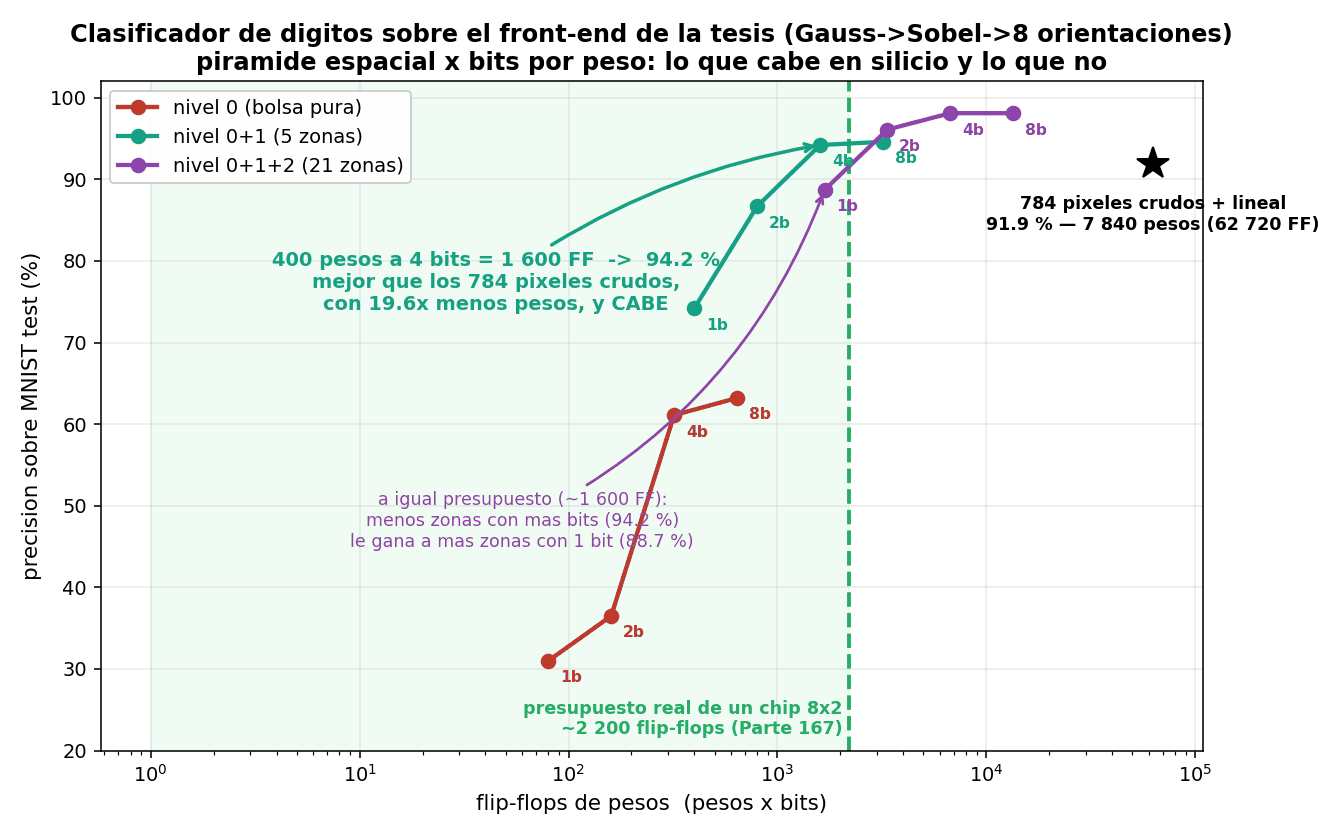
\includegraphics[keepaspectratio,alt={Figura 5.4. El espacio de diseño del clasificador, con el eje horizontal en escala logarítmica. Cada curva es un nivel de la pirámide espacial y cada punto una precisión de peso distinta. El hallazgo está en el cruce: 400 pesos de 4 bits ---1 600 biestables--- superan a los 784 píxeles crudos usando la vigésima parte de la memoria, y caben bajo el presupuesto real de un chip de 8×2 mosaicos, marcado con la línea vertical. A igualdad de memoria, la precisión de los pesos vale más que el número de zonas.}]{figuras/fig_5_4_espacio_de_diseno.png}}
\caption{\textbf{Figura 5.4.} El espacio de diseño del clasificador, con
el eje horizontal en escala logarítmica. Cada curva es un nivel de la
pirámide espacial y cada punto una precisión de peso distinta. El
hallazgo está en el cruce: \textbf{400 pesos de 4 bits ---1 600
biestables--- superan a los 784 píxeles crudos usando la vigésima parte
de la memoria}, y caben bajo el presupuesto real de un chip de 8×2
mosaicos, marcado con la línea vertical. A igualdad de memoria, la
precisión de los pesos vale más que el número de zonas.}
\end{figure}

\subsection{5.6.3 Lo que la exactitud no
muestra}\label{lo-que-la-exactitud-no-muestra}

Las medidas basadas en el \texttt{argmax} descartan la información de
los diez puntajes. Dos medidas que la conservan revelan una diferencia
que la exactitud oculta:

\begin{longtable}[]{@{}lrrr@{}}
\toprule\noalign{}
front-end & AUC macro & Brier & Brier skill \\
\midrule\noalign{}
\endhead
\bottomrule\noalign{}
\endlastfoot
SoC + Canny 1-salto & \textbf{0.9960} & \textbf{0.1465} &
\textbf{0.8371} \\
Canny 1-salto & 0.9957 & 0.1558 & 0.8268 \\
Sobel & 0.9945 & 0.1746 & 0.8059 \\
Canny transitivo & 0.9942 & \textbf{0.1991} & 0.7787 \\
SoC + Sobel & 0.9939 & 0.1749 & 0.8056 \\
\end{longtable}

El resultado de interés corresponde al Canny transitivo. En AUC ---que
mide el \textbf{ordenamiento}--- supera al SoC+Sobel; en Brier ---que
mide la \textbf{calibración}--- queda último por amplio margen.
\textbf{Ordena correctamente y decide mal.} Ello explica de forma
mecánica sus 139 falsos positivos: la reconstrucción morfológica
engruesa los contornos, el engrosamiento infla los histogramas, y el
criterio de rechazo ---que compara el mejor puntaje con el segundo---
deja hablar al circuito cuando debería callarlo.

\subsection{5.6.4 El punto de operación pesa más que el
front-end}\label{el-punto-de-operaciuxf3n-pesa-muxe1s-que-el-front-end}

Las comparaciones anteriores fijan el umbral y varían el filtro. El
experimento complementario ---fijar el filtro y \textbf{barrer el
umbral}--- arroja el resultado de mayor consecuencia práctica de esta
sección:

\begin{longtable}[]{@{}lrr@{}}
\toprule\noalign{}
magnitud & rango de exactitud & en unidades de σ \\
\midrule\noalign{}
\endhead
\bottomrule\noalign{}
\endlastfoot
el umbral, dentro del Sobel & \textbf{5.79 pp} & \textbf{4.4 σ} \\
el umbral, dentro del Canny & 0.90 pp & 0.7 σ \\
el filtro, cada uno en su óptimo & 0.38 pp & 0.3 σ \\
\end{longtable}

\textbf{Mover el umbral dentro del Sobel altera el resultado quince
veces más que cambiar de filtro.} Y la asimetría entre ambos front-ends
es el hallazgo: el Sobel presenta un óptimo estrecho ---su exactitud
recorre casi seis puntos a lo largo del rango útil--- mientras que el
Canny se mantiene en una meseta de nueve décimas. \textbf{El Canny en su
peor umbral supera al Sobel en diez de los once umbrales ensayados.}

El mecanismo reside en el algoritmo: el Sobel aplica un corte único y
nada recupera al píxel que queda por debajo; el Canny dispone de dos
umbrales y una histéresis que promueve el píxel débil adyacente a uno
fuerte. \textbf{La histéresis es un mecanismo de recuperación}, y de ahí
su insensibilidad.

\begin{quote}
\textbf{Consecuencia de diseño.} El front-end y el registro escribible
resuelven el mismo problema por vías distintas: el Canny adquiere
\textbf{en hardware} ---un \emph{line-buffer} adicional y ocho
comparaciones--- buena parte de la robustez que el Sobel obtiene
mediante \textbf{un procesador} capaz de reescribir el umbral. No son
decisiones que se sumen: son, en buena medida, \textbf{alternativas}.
\end{quote}

\subsection{5.6.5 El RTL contra el modelo, sobre el conjunto
completo}\label{el-rtl-contra-el-modelo-sobre-el-conjunto-completo}

Las cifras anteriores son del modelo en Python. La pregunta que decide
si sirven de algo es si el circuito las reproduce, y se respondió por el
camino más exigente disponible: \textbf{ejecutar el RTL sobre las diez
mil imágenes de prueba} en el simulador y comparar, no los porcentajes
agregados, sino cada predicción con la del modelo.

\begin{longtable}[]{@{}
  >{\raggedright\arraybackslash}p{(\linewidth - 2\tabcolsep) * \real{0.5000}}
  >{\raggedright\arraybackslash}p{(\linewidth - 2\tabcolsep) * \real{0.5000}}@{}}
\toprule\noalign{}
\begin{minipage}[b]{\linewidth}\raggedright
Comparación
\end{minipage} & \begin{minipage}[b]{\linewidth}\raggedright
Resultado
\end{minipage} \\
\midrule\noalign{}
\endhead
\bottomrule\noalign{}
\endlastfoot
Predicciones idénticas & \textbf{10 000 / 10 000} \\
Exactitud del RTL / del modelo & \textbf{91.04 \% / 91.04 \%} \\
Matriz de confusión & idéntica elemento por elemento \\
Veredictos de la clase de rechazo & \textbf{10 000 / 10 000}
idénticos \\
Cuadros aceptados · precisión al responder & 8 838 (88.38 \%) · 95.44
\%, en ambos \\
\end{longtable}

\begin{figure}
\centering
\pandocbounded{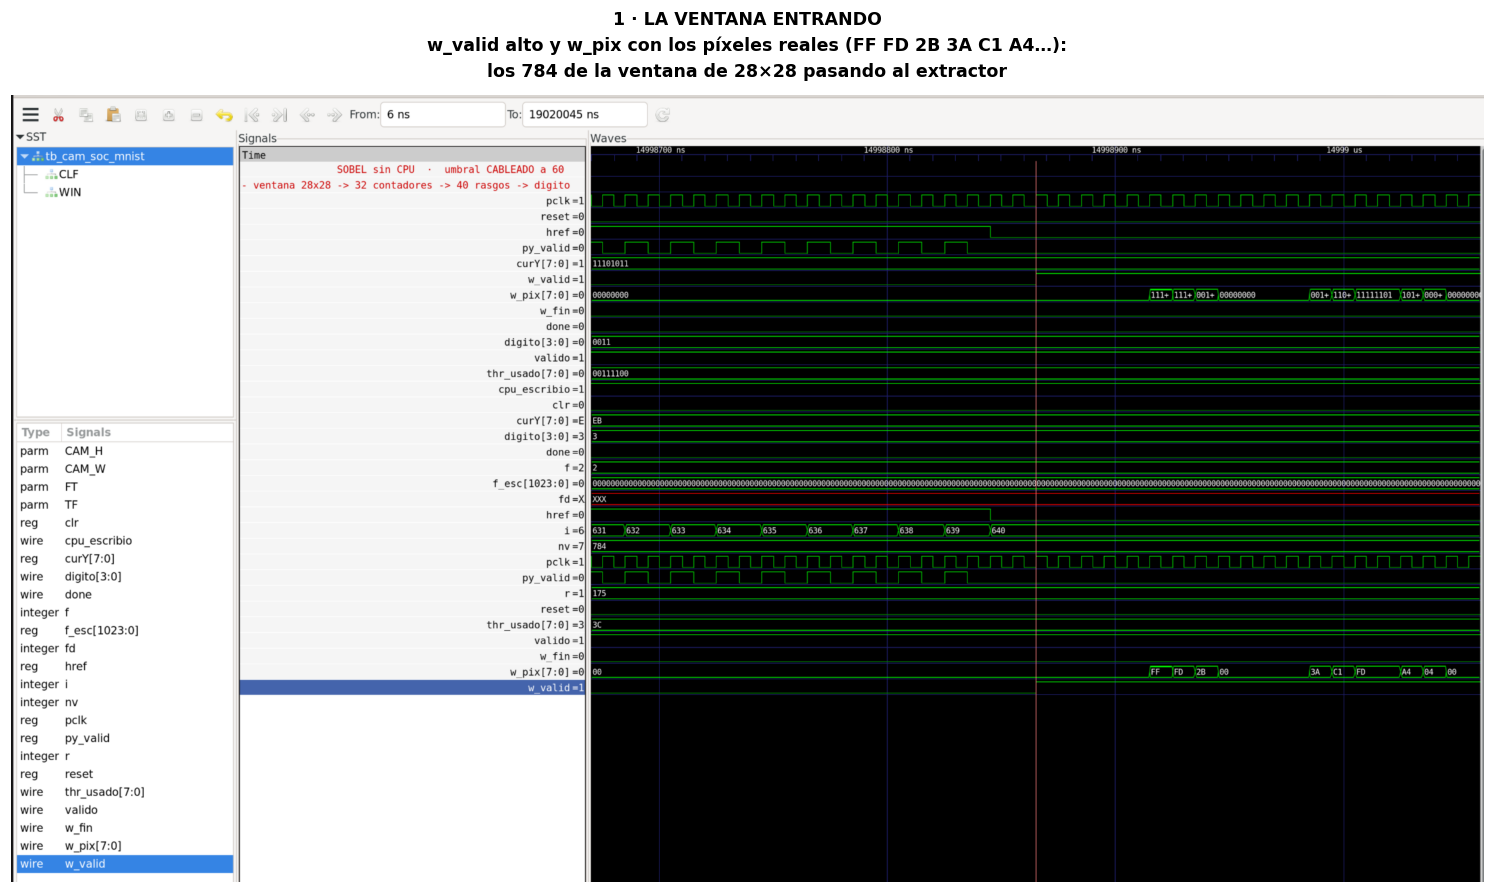
\includegraphics[keepaspectratio,alt={Figura 5.5. La ventana de 28×28 entrando al extractor, vista en el simulador. La señal w\_valid marca cada píxel válido y w\_pix lleva su valor ---FF FD 2B 3A C1 A4\ldots---; los 784 de la ventana pasan uno a uno antes de que done presente un dígito. Es el nivel al que se hizo la comparación contra el modelo: no se compararon porcentajes, se compararon señales.}]{figuras/fig_5_5_ventana_al_extractor.png}}
\caption{\textbf{Figura 5.5.} La ventana de 28×28 entrando al extractor,
vista en el simulador. La señal \texttt{w\_valid} marca cada píxel
válido y \texttt{w\_pix} lleva su valor
---\texttt{FF\ FD\ 2B\ 3A\ C1\ A4}\ldots---; los 784 de la ventana pasan
uno a uno antes de que \texttt{done} presente un dígito. Es el nivel al
que se hizo la comparación contra el modelo: no se compararon
porcentajes, se compararon señales.}
\end{figure}

No son cifras «parecidas» ni «dentro del margen de error»: \textbf{las
diez mil predicciones y los diez mil veredictos coinciden uno por uno},
y la matriz de confusión es la misma casilla por casilla. La
verificación de los filtros de la §5.1 se hizo sobre cinco imágenes;
ésta se hizo sobre diez mil, e incluye la decisión de rechazo, que es
lógica de comparación y no de aritmética.

\begin{quote}
Conviene precisar el alcance, porque más adelante aparece una cifra
distinta. Lo que aquí es exacto es el \textbf{clasificador completo}
---descriptor, pesos y decisión--- evaluado imagen por imagen. El 99.91
\% que informa la §5.6.6 se refiere a otra comparación: la del
\textbf{extractor de bordes} píxel a píxel dentro de la cadena, cuyas
discrepancias se concentran en la última fila del cuadro y no alteran
ninguna de las diez mil clasificaciones. Son dos medidas de objetos
distintos y no se contradicen.
\end{quote}

\subsection{5.6.6 Validación física}\label{validaciuxf3n-fuxedsica}

La validación sobre la placa se realizó en dos ensayos distintos, que
miden cosas distintas y cuyos resultados no deben confundirse.

\begin{figure}
\centering
\pandocbounded{
\includegraphics[keepaspectratio,alt={Figura 5.6. La cadena completa ---cámara, procesador, filtro y clasificador--- en señales, sobre la escena del dígito 3. El panel A muestra los 19 ms de dos cuadros: el veredicto sale en el primero y no cambia en el segundo. El panel B captura el instante en que el procesador sustituye el umbral por omisión del RTL, 110, por el 90 que escribe el firmware, con el camino de datos todavía en reinicio. El panel C mide los 639,5 µs que tardan las 400 multiplicaciones-acumulaciones y el argmax.}]{figuras/fig_5_6_cadena_en_senales.png}}
\caption{\textbf{Figura 5.6.} La cadena completa ---cámara, procesador,
filtro y clasificador--- en señales, sobre la escena del dígito 3. El
panel A muestra los 19 ms de dos cuadros: el veredicto sale en el
primero y no cambia en el segundo. El panel B captura el instante en que
\textbf{el procesador sustituye el umbral por omisión del RTL, 110, por
el 90 que escribe el firmware}, con el camino de datos todavía en
reinicio. El panel C mide los 639,5 µs que tardan las 400
multiplicaciones-acumulaciones y el \texttt{argmax}.}
\end{figure}

\textbf{Primer ensayo: diez dígitos grabados en el propio bitstream.} Se
embebieron diez imágenes de MNIST en la memoria de configuración y se
hizo que el circuito informara sus veredictos por el puerto serie, sin
cámara. La placa acertó \textbf{ocho de los diez}, y lo relevante no son
los ocho aciertos sino los dos fallos: el circuito confunde el
\textbf{2} con un 0 y el \textbf{3} con un 8, \textbf{exactamente los
mismos dos dígitos y exactamente las mismas respuestas equivocadas} que
había dado la simulación del diseño completo. Ninguno de los diez cambió
de respuesta a lo largo de unas treinta repeticiones.

\begin{quote}
Reproducir un acierto puede ser casualidad; reproducir un error
específico y repetido, no. Este ensayo no mide la exactitud del sistema
---diez imágenes no son una medida estadística--- sino que
\textbf{cierra el último eslabón de la traducción}: el diseño
sintetizado, emplazado, ruteado y cargado en silicio se comporta como el
RTL verificado, errores incluidos.
\end{quote}

\begin{figure}
\centering
\pandocbounded{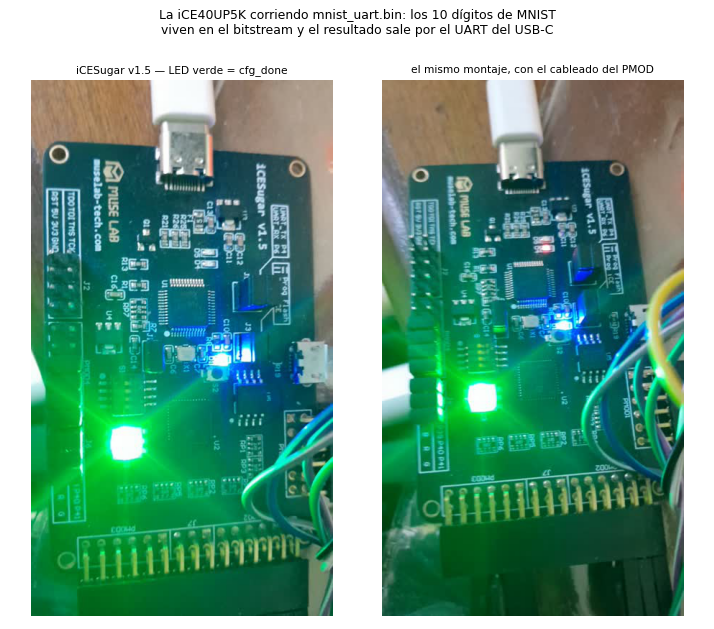
\includegraphics[keepaspectratio,alt={Figura 5.7. La tarjeta durante ese primer ensayo, con el mapa de bits cargado. El diodo verde está cableado a la señal de configuración terminada; el azul parpadea con el latido del sistema. Los diez veredictos salen por el puerto serie del mismo conector que alimenta la tarjeta. A la derecha, el mismo montaje con el cableado del módulo de pantalla ya conectado.}]{figuras/fig_5_7_la_placa_uart.png}}
\caption{\textbf{Figura 5.7.} La tarjeta durante ese primer ensayo, con
el mapa de bits cargado. El diodo verde está cableado a la señal de
configuración terminada; el azul parpadea con el latido del sistema. Los
diez veredictos salen por el puerto serie del mismo conector que
alimenta la tarjeta. A la derecha, el mismo montaje con el cableado del
módulo de pantalla ya conectado.}
\end{figure}

\textbf{Segundo ensayo: dígitos manuscritos ante la cámara.} El sistema
completo ---procesador RISC-V, periférico de umbrales, front-end Canny y
clasificador--- se enfrentó a dígitos escritos a mano y captados por una
cámara OV7670. \textbf{El circuito reconoció nueve de diez dígitos},
coincidiendo exactamente con lo que la simulación había predicho para
esa configuración.

Ese acuerdo, sin embargo, no se obtuvo al primer intento, y la causa
merece registrarse porque es la única discrepancia entre simulación y
silicio de todo el trabajo. En la primera versión la placa respondía
\textbf{ocho de diez} mientras la simulación sostenía nueve. El umbral
inferior del front-end se leía desde el módulo de control mediante una
\textbf{referencia jerárquica} ---\texttt{SOC.flt\_tlo}--- en lugar de
un puerto declarado. Ambas herramientas aceptaron el archivo sin una
sola advertencia y construyeron circuitos distintos: \texttt{iverilog}
resuelve la referencia y simula con el umbral escrito por el procesador,
mientras que el sintetizador crea un cable implícito de un bit que nadie
gobierna y fija el umbral inferior en cero. Sustituida la referencia por
un \textbf{puerto real}, la placa pasó a nueve de diez: el valor que la
simulación predecía.

\begin{quote}
\textbf{La lección no es que hubiera un error, sino dónde estaba.} El
RTL era legal, la simulación era correcta y la síntesis también lo era;
lo que falló fue suponer que ambas leían la misma descripción. Una
construcción que el lenguaje admite y que las dos herramientas
interpretan de forma distinta es indetectable por inspección y
silenciosa en los registros de ambas. Se deja escrita la regla de
trabajo que se adoptó a partir de aquí: \textbf{toda señal que cruce una
frontera de módulo se declara como puerto}, aunque el simulador acepte
el atajo.
\end{quote}

La verificación del extractor contra su modelo de referencia arrojó
\textbf{99.91 \%} de coincidencia exacta píxel a píxel para el Sobel y
\textbf{99.93 \%} para el Canny, concentrándose las diferencias en la
última fila del cuadro.

\subsection{5.6.7 Implementación en
silicio}\label{implementaciuxf3n-en-silicio}

El reconocedor se llevó a tecnología \texttt{sky130\_fd\_sc\_hd} en dos
variantes, ejecutando el flujo completo de OpenLane hasta la firma del
GDS:

\begin{longtable}[]{@{}lrr@{}}
\toprule\noalign{}
magnitud & Sobel & Canny 1-salto \\
\midrule\noalign{}
\endhead
\bottomrule\noalign{}
\endlastfoot
área del \emph{die} & 0.845 mm² & 0.890 mm² \\
celdas tras síntesis & 16 718 & 17 373 \\
celdas emplazadas & 19 949 & 20 921 \\
período de reloj & 30 ns (33.3 MHz) & 30 ns (33.3 MHz) \\
holgura con parásitos (\texttt{spef\_wns}) & \textbf{0.00 ns} &
\textbf{0.00 ns} \\
DRC · LVS · XOR & 0 · 0 · 0 & 0 · 0 · 0 \\
\end{longtable}

Ambos circuitos cierran el temporizado con los parásitos del
interconexionado extraídos y superan las tres verificaciones de firma
sin observaciones. Merece señalarse que \textbf{cierran más rápido que
los circuitos de visión equivalentes} ---que requirieron 32 y 36 ns---,
lo que resulta coherente con la ausencia de memoria de cuadro: es el
multiplexor de lectura del \emph{framebuffer} el que constituye el
camino crítico de aquéllos.

\textbf{Son los primeros circuitos de este trabajo cuya salida no es una
imagen.} Los diez presentados en las secciones §5.3 y §5.4 procesan;
éstos reconocen.

\subsection{5.6.8 El costo relativo del front-end depende del
sistema}\label{el-costo-relativo-del-front-end-depende-del-sistema}

La comparación de área entre ambos front-ends admite cuatro niveles de
integración. Las cuatro filas están en \textbf{celdas emplazadas}, la
misma escala de la §5.3, de modo que los cocientes son directamente
comparables entre sí:

\begin{longtable}[]{@{}
  >{\raggedright\arraybackslash}p{(\linewidth - 6\tabcolsep) * \real{0.2000}}
  >{\raggedleft\arraybackslash}p{(\linewidth - 6\tabcolsep) * \real{0.2667}}
  >{\raggedleft\arraybackslash}p{(\linewidth - 6\tabcolsep) * \real{0.2667}}
  >{\raggedleft\arraybackslash}p{(\linewidth - 6\tabcolsep) * \real{0.2667}}@{}}
\toprule\noalign{}
\begin{minipage}[b]{\linewidth}\raggedright
nivel
\end{minipage} & \begin{minipage}[b]{\linewidth}\raggedleft
Sobel
\end{minipage} & \begin{minipage}[b]{\linewidth}\raggedleft
Canny
\end{minipage} & \begin{minipage}[b]{\linewidth}\raggedleft
factor
\end{minipage} \\
\midrule\noalign{}
\endhead
\bottomrule\noalign{}
\endlastfoot
filtro aislado & 5 823 & 12 993 & \textbf{2.23×} \\
con procesador & 12 043 & 22 054 & 1.83× \\
sistema de visión completo & 35 653 & 41 925 & 1.18× \\
reconocedor con procesador & 19 949 & 20 921 & 1.05× \\
\textbf{reconocedor que además muestra} & \textbf{38 643} & \textbf{39
794} & \textbf{1.03×} \\
\end{longtable}

\textbf{El sobrecosto del Canny se diluye conforme crece el sistema que
lo rodea.} Considerado de forma aislada cuesta un \textbf{123 \%} más;
con un procesador al lado, un 83 \%; dentro de un sistema de visión, un
18 \%; integrado en un reconocedor, un 5 \%; y en un reconocedor que
además dibuja en pantalla, un \textbf{3 \%}. El motivo es que el
clasificador ---histograma, pirámide y 400 multiplicaciones--- es
idéntico en ambas variantes y domina el área, mientras que la diferencia
se reduce al tercer \emph{line-buffer}.

De ello se sigue una conclusión condicional: \textbf{el Sobel aventaja
al Canny en área únicamente cuando el filtro constituye el circuito
completo.} En un sistema que reconoce, esa ventaja ---la única que el
Sobel conserva, según §5.6.2 a §5.6.4--- deja de ser determinante.

\begin{center}\rule{0.5\linewidth}{0.5pt}\end{center}

\subsection{Referencias de la
sección}\label{referencias-de-la-secciuxf3n}

\begin{itemize}
\tightlist
\item
  Chow, C. K. (1970). \emph{On Optimum Recognition Error and Reject
  Tradeoff.} IEEE Trans. Inf. Theory, 16(1), 41-46.
\item
  Dalal, N. y Triggs, B. (2005). \emph{Histograms of Oriented Gradients
  for Human Detection.} CVPR, 886-893.
\item
  Lazebnik, S., Schmid, C. y Ponce, J. (2006). \emph{Beyond Bags of
  Features: Spatial Pyramid Matching.} CVPR, 2169-2178.
\item
  Lowe, D. G. (2004). \emph{Distinctive Image Features from
  Scale-Invariant Keypoints.} IJCV, 60(2), 91-110.
\end{itemize}

\section{5.7 Verificación eléctrica del camino
crítico}\label{verificaciuxf3n-eluxe9ctrica-del-camino-cruxedtico}

\begin{quote}
\textbf{Estado:} borrador 1, 2026-09-21. Fuente: cuaderno 2, §33. Todas
las cifras de esta sección proceden de corridas de NGSpice sobre
\texttt{sky130\_fd\_sc\_hd} en la esquina típica, 1,8 V y 25 °C, y de
los ficheros de parásitos extraídos de los dos reconocedores.
\end{quote}

Las secciones anteriores aceptaron sin discusión lo que el analizador de
tiempos informa. Ésta pregunta si ese número es correcto, y lo hace por
el único camino que no depende de la misma herramienta: \textbf{resolver
los transistores}.

La pregunta no es ociosa. Un analizador estático no simula: consulta
tablas caracterizadas de antemano e interpola. Es rapidísimo y es lo que
permite firmar un circuito de doscientas mil instancias, pero entre su
respuesta y la física median un modelo de celda, un modelo de cable y un
procedimiento de interpolación. Comprobar cuánto de lo que informa
sobrevive a una simulación eléctrica es, por tanto, una verificación del
instrumento y no del circuito.

\subsection{5.7.1 Por qué el camino crítico y no el
chip}\label{por-quuxe9-el-camino-cruxedtico-y-no-el-chip}

Simular los dos reconocedores enteros no es inviable por tamaño
---\texttt{pan\_sobel} tiene 116 314 transistores y en este trabajo ya
se simuló un procesador de 121 310--- sino \textbf{por tiempo}: para que
el clasificador vea sus 784 píxeles hay que hacerle entrar un cuadro
completo, y eso son 633 800 ciclos, unos treinta y dos veces más
actividad que la simulación de procesador ya realizada.

El camino crítico, en cambio, son \textbf{treinta y siete celdas} en un
chip y treinta y seis en el otro. Se extrajeron del reporte del
analizador, se reconstruyeron como cadena aislada con la carga y la
pendiente que el propio reporte declara en cada etapa, y se resolvieron
en NGSpice.

\subsection{5.7.2 El resultado}\label{el-resultado}

Se aplicaron cinco variantes del mismo banco, cada una añadiendo un
ingrediente al anterior, de modo que la diferencia entre dos renglones
consecutivos aísla la contribución de ese ingrediente:

\begin{longtable}[]{@{}
  >{\raggedright\arraybackslash}p{(\linewidth - 4\tabcolsep) * \real{0.2727}}
  >{\raggedleft\arraybackslash}p{(\linewidth - 4\tabcolsep) * \real{0.3636}}
  >{\raggedleft\arraybackslash}p{(\linewidth - 4\tabcolsep) * \real{0.3636}}@{}}
\toprule\noalign{}
\begin{minipage}[b]{\linewidth}\raggedright
\end{minipage} & \begin{minipage}[b]{\linewidth}\raggedleft
\texttt{pan\_sobel} (37 etapas)
\end{minipage} & \begin{minipage}[b]{\linewidth}\raggedleft
\texttt{pan\_canny} (36 etapas)
\end{minipage} \\
\midrule\noalign{}
\endhead
\bottomrule\noalign{}
\endlastfoot
\textbf{Analizador estático, con parásitos} & \textbf{12,230 ns} &
\textbf{9,890 ns} \\
A · las puertas solas & 4,646 ns & 4,424 ns \\
B · más la capacitancia extraída, agrupada & 8,159 ns & 7,552 ns \\
C · más la pendiente de entrada real & 8,178 ns & 7,588 ns \\
D0 · más la topología del fichero de parásitos, \textbf{con R = 0} &
7,603 ns & 7,022 ns \\
D · más la \textbf{resistencia medida} de cada tramo & 7,620 ns & 7,043
ns \\
E · más la \textbf{celda extraída del \emph{layout}} & \textbf{9,694 ns}
& \textbf{8,962 ns} \\
\emph{fracción del retardo que la simulación reproduce} & \emph{79,3 \%}
& \emph{90,6 \%} \\
\end{longtable}

La variante \textbf{D0 es un control}, idéntica a la D salvo en que sus
resistencias valen cero. Sin ella, el efecto de la resistencia y el de
\emph{repartir} la capacitancia a lo largo del árbol en vez de agruparla
en un nodo quedarían sumados en una sola cifra y no podrían separarse.

\begin{figure}
\centering
\pandocbounded{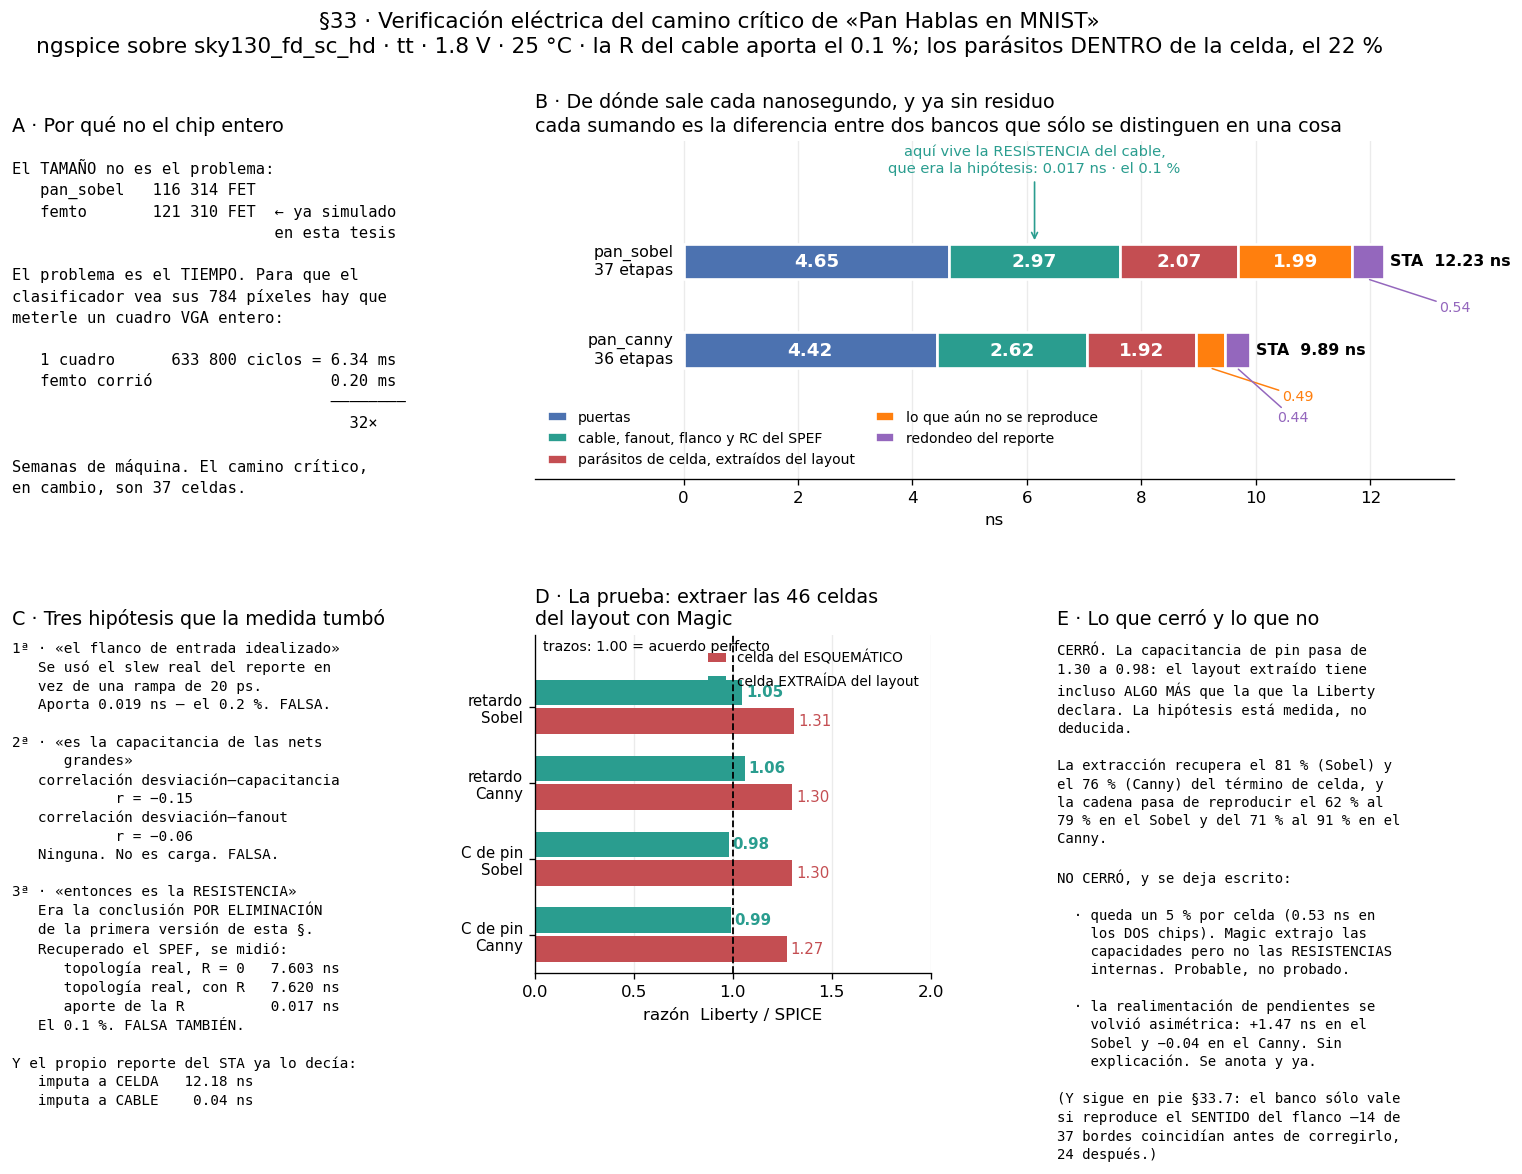
\includegraphics[keepaspectratio,alt={Figura 5.8. El desglose completo de la verificación. El panel A explica por qué se simula el camino y no el chip; el B reparte los 12,23 ns del pan\_sobel y los 9,89 del pan\_canny en sumandos que no dejan residuo; el C recoge las tres hipótesis que la medida desmintió; el D contrapone la celda del esquemático con la extraída del dibujo en los dos experimentos independientes; y el E separa lo que quedó cerrado de lo que se deja escrito como abierto.}]{figuras/fig_5_8_spice_desglose.png}}
\caption{\textbf{Figura 5.8.} El desglose completo de la verificación.
El panel A explica por qué se simula el camino y no el chip; el B
reparte los 12,23 ns del \texttt{pan\_sobel} y los 9,89 del
\texttt{pan\_canny} en sumandos que no dejan residuo; el C recoge las
tres hipótesis que la medida desmintió; el D contrapone la celda del
esquemático con la extraída del dibujo en los dos experimentos
independientes; y el E separa lo que quedó cerrado de lo que se deja
escrito como abierto.}
\end{figure}

\subsection{5.7.3 Tres explicaciones que la medida
desmintió}\label{tres-explicaciones-que-la-medida-desmintiuxf3}

Las tres parecían razonables, y conviene dejar constancia de las tres.

\textbf{El flanco de entrada idealizado.} El estímulo inicial era una
rampa de 20 ps, mucho más limpia que la transición que la primera etapa
recibe en el circuito; cabía esperar que un frente degradado se
propagase como retardo a lo largo de las treinta y siete etapas.
Sustituido por la pendiente real que el reporte declara, la contribución
resultó de \textbf{0,019 ns: el 0,2 \%}.

\textbf{La capacitancia de las redes grandes.} Las desviaciones mayores
se concentraban en puertas de muchas entradas, lo que sugería redes
largas y cargadas. Se midió la correlación entre la desviación de cada
etapa y su capacitancia: \textbf{r = −0,15}; y con el número de
destinos: \textbf{r = −0,06}. Ninguna de las dos sostiene la
explicación.

\textbf{La resistencia de la interconexión.} Descartadas las anteriores
quedaba ésta, y \textbf{así se dio por concluida la primera versión de
esta sección}: el analizador trabaja sobre el fichero de parásitos, que
informa resistencia y capacitancia de cada red, mientras que el reporte
de texto publica sólo la capacitancia, de modo que la simulación habría
recibido una descripción incompleta de los cables. La conjetura no pudo
comprobarse entonces porque ese fichero no se había conservado.

Recuperado, se midió. \textbf{La resistencia de la interconexión aporta
0,017 ns: el 0,1 \% del camino.} No los cuatro nanosegundos que había
que explicar.

\begin{quote}
\textbf{El propio reporte lo decía, y no se leyó.} El analizador imputa
cada retardo a un pin, y los de pin de salida son de celda mientras que
los de pin de entrada son de cable. Sumados por separado a lo largo del
camino: \textbf{12,18 ns imputados a celda y 0,04 ns a cable}. La
herramienta nunca atribuyó el tiempo a la interconexión. Bastaba con
sumar dos columnas.
\end{quote}

\subsection{5.7.4 La causa: la celda del esquemático no es la celda del
silicio}\label{la-causa-la-celda-del-esquemuxe1tico-no-es-la-celda-del-silicio}

Si la diferencia está dentro de las celdas, hay que preguntárselo a una
celda sola. El banco se redujo al mínimo ---una celda, el arco que el
camino recorre, la pendiente y la carga que el reporte declara--- y se
hizo la misma pregunta dos veces: a la tabla caracterizada, interpolando
como hace el analizador, y al simulador, resolviendo los transistores
que el kit de diseño distribuye.

La tabla reproduce al analizador casi exactamente, lo que confirma que
éste se limita a consultarla. La simulación, en cambio, queda
\textbf{sistemáticamente por debajo en treinta y cinco de las treinta y
siete etapas}, con una razón de \textbf{1,31} que no depende ni de la
carga ni de la pendiente. Esa independencia es la que descarta un
defecto del banco y señala a la celda misma.

La causa está en el fichero que se le entregó como modelo. El kit
distribuye el netlist \textbf{esquemático}: doce transistores y ni un
solo parásito. La biblioteca caracterizada, en cambio, se obtuvo sobre
la celda \textbf{dibujada}, con el metal, los contactos y la difusión
que el \emph{layout} añade. Al simulador se le describió la celda antes
de dibujarla.

Eso admite medición directa. Inyectando una rampa lenta en cada pin de
entrada e integrando la corriente ---capacitancia como carga dividida
por tensión, sin modelo ni supuesto--- la biblioteca atribuye a cada
pin, en promedio sobre los treinta y cinco del camino, \textbf{un 30 \%
más de capacitancia de la que el esquemático tiene}.

\begin{quote}
\textbf{Dos experimentos distintos, la misma cifra.} La razón entre el
retardo que la biblioteca declara y el que la simulación obtiene sobre
el esquemático es \textbf{1,31}. La razón entre la capacitancia que la
biblioteca declara y la que el esquemático tiene es \textbf{1,30}. Uno
mide tiempos y el otro mide carga, sobre las mismas treinta y siete
etapas.
\end{quote}

\textbf{La comprobación.} Lo anterior establece que al esquemático le
faltan parásitos, no que sean \emph{ésos} los que faltan. El kit no
distribuye el netlist de la celda dibujada, pero sí el dibujo: se
extrajeron con Magic las \textbf{cuarenta y seis celdas} que aparecen en
los dos caminos y se repitieron los dos experimentos sin cambiar nada
más.

\begin{longtable}[]{@{}
  >{\raggedright\arraybackslash}p{(\linewidth - 4\tabcolsep) * \real{0.2727}}
  >{\raggedleft\arraybackslash}p{(\linewidth - 4\tabcolsep) * \real{0.3636}}
  >{\raggedleft\arraybackslash}p{(\linewidth - 4\tabcolsep) * \real{0.3636}}@{}}
\toprule\noalign{}
\begin{minipage}[b]{\linewidth}\raggedright
razón biblioteca / simulación
\end{minipage} & \begin{minipage}[b]{\linewidth}\raggedleft
celda del \textbf{esquemático}
\end{minipage} & \begin{minipage}[b]{\linewidth}\raggedleft
celda \textbf{extraída}
\end{minipage} \\
\midrule\noalign{}
\endhead
\bottomrule\noalign{}
\endlastfoot
capacitancia de pin · \texttt{pan\_sobel} & 1,30 & \textbf{0,98} \\
capacitancia de pin · \texttt{pan\_canny} & 1,27 & \textbf{0,99} \\
retardo de celda aislada · \texttt{pan\_sobel} & 1,31 & \textbf{1,05} \\
retardo de celda aislada · \texttt{pan\_canny} & 1,30 & \textbf{1,06} \\
\end{longtable}

\textbf{La discrepancia de capacitancia desaparece.} La hipótesis queda
medida y no deducida, que era justamente lo que faltaba.

\subsection{5.7.5 La cuenta, y lo que queda
abierto}\label{la-cuenta-y-lo-que-queda-abierto}

Repartidos los 12,230 ns sin residuo, el término que importa sale igual
en los dos circuitos:

\begin{longtable}[]{@{}
  >{\raggedright\arraybackslash}p{(\linewidth - 4\tabcolsep) * \real{0.2727}}
  >{\raggedleft\arraybackslash}p{(\linewidth - 4\tabcolsep) * \real{0.3636}}
  >{\raggedleft\arraybackslash}p{(\linewidth - 4\tabcolsep) * \real{0.3636}}@{}}
\toprule\noalign{}
\begin{minipage}[b]{\linewidth}\raggedright
\end{minipage} & \begin{minipage}[b]{\linewidth}\raggedleft
\texttt{pan\_sobel}
\end{minipage} & \begin{minipage}[b]{\linewidth}\raggedleft
\texttt{pan\_canny}
\end{minipage} \\
\midrule\noalign{}
\endhead
\bottomrule\noalign{}
\endlastfoot
\textbf{el modelo de celda, como fracción del camino} & \textbf{22,6 \%}
& \textbf{22,1 \%} \\
resistencia de la interconexión & 0,1 \% & 0,2 \% \\
\end{longtable}

Dos circuitos distintos, dos caminos críticos que no comparten una sola
instancia, y la misma cifra a cuatro décimas de punto: \textbf{algo más
de la quinta parte del retardo de un camino crítico la ponen los
parásitos que el dibujo añade dentro de las celdas.}

\begin{figure}
\centering
\pandocbounded{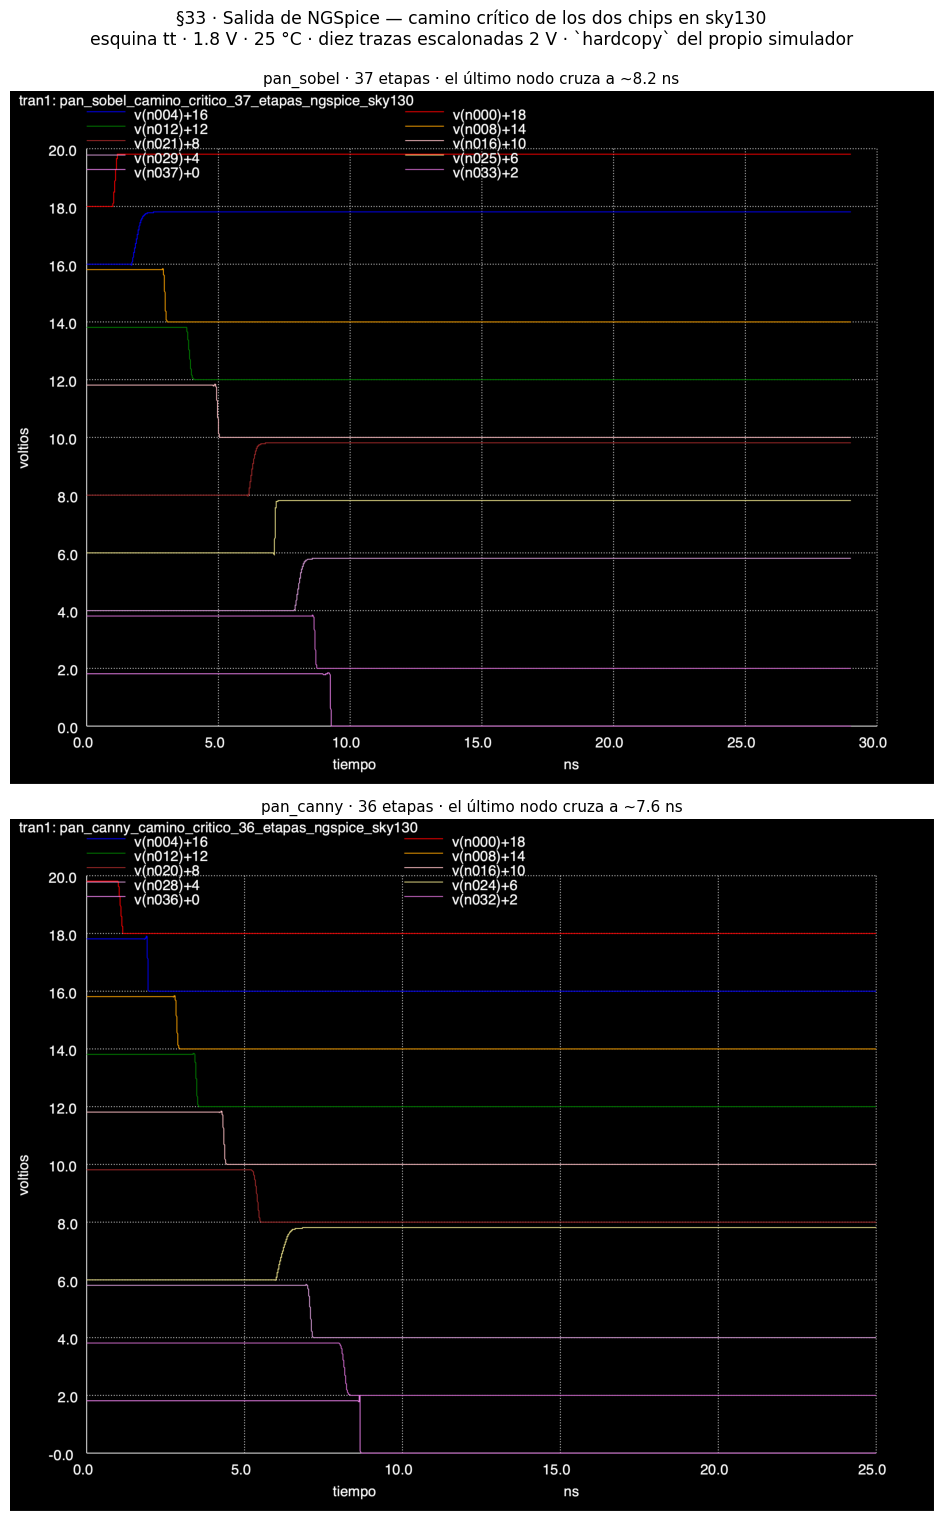
\includegraphics[keepaspectratio,alt={Figura 5.9. La salida del simulador, tal como éste la dibuja. Cada traza es un nodo del camino crítico, desplazada dos voltios respecto de la anterior para que las diez quepan en el mismo eje; la cascada de transiciones de arriba abajo es la señal propagándose etapa por etapa. El último nodo del pan\_sobel conmuta a unos 8,2 ns y el del pan\_canny a unos 7,6, que son las variantes D de la tabla anterior.}]{figuras/fig_5_9_spice_ondas.png}}
\caption{\textbf{Figura 5.9.} La salida del simulador, tal como éste la
dibuja. Cada traza es un nodo del camino crítico, desplazada dos voltios
respecto de la anterior para que las diez quepan en el mismo eje; la
cascada de transiciones de arriba abajo es la señal propagándose etapa
por etapa. El último nodo del \texttt{pan\_sobel} conmuta a unos 8,2 ns
y el del \texttt{pan\_canny} a unos 7,6, que son las variantes D de la
tabla anterior.}
\end{figure}

\textbf{Lo que no cerró, y se deja escrito.} Queda un 5 \% por celda
---0,528 ns en un chip y 0,530 en el otro, prácticamente el mismo valor
absoluto en dos caminos distintos--- que la extracción no recupera. La
explicación más probable es que el procedimiento empleado conserva las
\textbf{capacidades} internas de la celda pero no sus
\textbf{resistencias}, de modo que su metal interno sigue comportándose
como un cortocircuito ideal. Se anota como \textbf{probable y no
comprobada}. Y la realimentación de pendientes a lo largo de la cadena
resulta asimétrica entre los dos chips ---+1,47 ns en uno y −0,04 en el
otro--- sin explicación disponible.

\begin{quote}
\textbf{La conclusión.} El simulador y el analizador no discrepan sobre
la física: discrepan sobre el circuito. Al analizador se le describió la
celda tal como quedó en el \emph{layout}; al simulador, tal como estaba
en el esquema.

La verificación eléctrica no midió, por tanto, que el analizador se
equivocara. Midió \textbf{cuánto del retardo de un circuito integrado lo
pone el dibujo y no el esquema}: algo más de la quinta parte, y la misma
fracción en dos chips independientes. Es una cifra más útil que la que
se buscaba, y explica por qué ninguna implementación puede firmarse
sobre el esquemático.
\end{quote}

\chapter{6. Discusión}\label{discusiuxf3n}

\begin{quote}
\textbf{Estado:} borrador 1, escrito el 2026-09-21. Fuente: cuadernos 1
y 2, y el Capítulo 5. Formato Markdown para convertir con
\texttt{pandoc}.
\end{quote}

El capítulo anterior presentó mediciones. Éste sostiene afirmaciones. La
diferencia importa: una medición es un hecho que se comprueba repitiendo
el experimento, mientras que una afirmación es una lectura de varios
hechos y puede ser equivocada aunque todos ellos sean correctos. Este
trabajo tuvo que retractar dos afirmaciones de ese tipo durante su
desarrollo, y la experiencia dejó una disciplina que se aplica aquí:
\textbf{cada tesis de este capítulo señala qué medición la sostiene y
qué otra lectura descarta.}

\section{6.1 Lo que decide si un algoritmo cabe no es el
algoritmo}\label{lo-que-decide-si-un-algoritmo-cabe-no-es-el-algoritmo}

Ésta es la afirmación central del trabajo, y la más contraintuitiva para
quien llega desde el software.

Los tres filtros implementados ejecutan aritmética comparable. Ninguno
multiplica; los tres recorren la imagen aplicando una ventana de 3×3 y
comparando contra un umbral. Si el costo en silicio siguiera a la
complejidad aritmética, los tres deberían costar aproximadamente lo
mismo. La §5.4.3 midió lo contrario:

\begin{longtable}[]{@{}llr@{}}
\toprule\noalign{}
desde & hasta & cuesta \\
\midrule\noalign{}
\endhead
\bottomrule\noalign{}
\endlastfoot
Sobel & Canny de un salto & \textbf{+5 851 celdas} \\
Canny de un salto & Canny transitivo & \textbf{+94 511 celdas} \\
\end{longtable}

Ampliar el alcance de la ventana en un salto cuesta menos de seis mil
celdas. Ampliarlo al cuadro completo cuesta \textbf{noventa y cuatro mil
quinientas once}. Y la causa no está en las operaciones sino en
\textbf{cuánto estado hay que sostener a la vez}: los dos primeros
filtros procesan en flujo y retienen unas pocas líneas; el tercero
necesita el cuadro entero residente y accesible en orden arbitrario,
porque su punto fijo puede propagar una decisión desde cualquier píxel
hacia cualquier otro.

La comparación que resume el capítulo es ésta: \textbf{un procesador
RISC-V completo, con su memoria de programa y su periférico, cuesta
alrededor de nueve mil celdas} ---medido tres veces, sobre los tres
filtros, con una dispersión inferior al 5 \%--- \textbf{es decir,
aproximadamente la décima parte de lo que cuesta cambiar el alcance del
patrón de local a global.}

\begin{quote}
Dicho de otro modo: en el presupuesto de este chip, \textbf{meter un
procesador entero es una decisión menor comparada con decidir cuánta
imagen mira el filtro}. Es exactamente lo contrario de lo que sugiere la
intuición formada en software, donde el procesador es el recurso caro y
la memoria se pide al sistema operativo.
\end{quote}

\subsection{Las tres caras del mismo
precio}\label{las-tres-caras-del-mismo-precio}

El costo de la memoria no se cobra sólo en área. La §5.4.1 muestra que
\textbf{los dos circuitos transitivos son también los dos únicos que no
cierran temporizado}, con −19,35 ns y −18,23 ns de holgura una vez
extraídos los parásitos. El multiplexor que lee un framebuffer de miles
de entradas es un camino largo por construcción, y a partir de cierto
tamaño deja de ser caro para volverse inviable.

Y se cobra en manufacturabilidad. La §5.3 documenta que los diseños con
framebuffer grande acumulan un número de violaciones de antena muy
superior al resto, porque las redes de direccionamiento son largas y
ramificadas.

\textbf{Área, frecuencia y manufacturabilidad son tres manifestaciones
del mismo hecho}, y conviene presentarlas juntas: un diseñador que
optimice sólo el área concluirá que el framebuffer es aceptable, porque
sólo verá un tercio del problema.

\section{6.2 El costo se movió; no se
eliminó}\label{el-costo-se-moviuxf3-no-se-eliminuxf3}

Una lectura apresurada del clasificador de la §5.6 sugeriría que la
solución al problema anterior es sustituir memoria por lógica. El
trabajo permite matizar eso con números propios.

El clasificador de dígitos alcanza 91,04 \% sobre MNIST con \textbf{400
pesos de cuatro bits} ---doscientos bytes--- frente al 91,9 \% que
obtienen los 784 píxeles crudos con 7 840 pesos. La memoria se redujo en
un factor de veinte y la exactitud no se movió. Es un resultado fuerte,
y se enuncia así en la §5.6.

Pero el descriptor que hace posible esa reducción ---histograma de
orientaciones por zona, sobre bordes--- \textbf{no es gratuito}: hay que
calcularlo, y calcularlo es lógica. Las etapas cableadas que lo producen
cuestan decenas de miles de celdas.

\begin{quote}
La conclusión honesta no es «la codificación inteligente elimina el
costo» sino \textbf{«la codificación inteligente mueve el costo de
memoria a lógica»}, y eso es valioso únicamente porque en este sustrato
la memoria es el recurso caro. En una FPGA con bloques de memoria
disponibles, la misma decisión sería indiferente o incluso perjudicial.
\end{quote}

\section{6.3 Quién fija el reloj cambia con lo que se mete en el
chip}\label{quiuxe9n-fija-el-reloj-cambia-con-lo-que-se-mete-en-el-chip}

Los resultados del Capítulo 5 permiten seguir el camino crítico a lo
largo de una familia de diseños y observar que \textbf{el responsable
cambia tres veces}:

\begin{longtable}[]{@{}
  >{\raggedright\arraybackslash}p{(\linewidth - 2\tabcolsep) * \real{0.5000}}
  >{\raggedright\arraybackslash}p{(\linewidth - 2\tabcolsep) * \real{0.5000}}@{}}
\toprule\noalign{}
\begin{minipage}[b]{\linewidth}\raggedright
Diseño
\end{minipage} & \begin{minipage}[b]{\linewidth}\raggedright
Quién fija la frecuencia
\end{minipage} \\
\midrule\noalign{}
\endhead
\bottomrule\noalign{}
\endlastfoot
Filtros solos & el camino de datos del filtro \\
Con procesador & \textbf{el FemtoRV32} \\
Con framebuffer grande & \textbf{el multiplexor de lectura del
framebuffer} \\
\end{longtable}

Es un resultado útil para quien planifique un sistema parecido, porque
implica que \textbf{optimizar el bloque que fue crítico en el diseño
anterior puede no mejorar nada}. La pregunta «¿qué limita mi
frecuencia?» no tiene una respuesta estable: tiene una respuesta por
configuración.

\section{6.4 Integrar no es sumar, pero sólo cuando el temporizado
aprieta}\label{integrar-no-es-sumar-pero-suxf3lo-cuando-el-temporizado-aprieta}

Dos observaciones de este trabajo parecen contradecirse, y el matiz está
en la diferencia.

Al integrar el procesador con el filtro Canny en un die apretado, el
resultado superó la predicción ingenua ---la suma de las partes--- en
unas 6 500 celdas. En otro diseño de la misma familia, con die holgado y
reloj relajado, el resultado quedó un \textbf{1,6 \% por debajo} de esa
predicción.

Las dos medidas son correctas. Lo que las separa es \textbf{si el flujo
tuvo que trabajar para cerrar temporizado}: cuando lo tuvo, insertó
amortiguadores y redimensionó celdas, y ese trabajo se cobra en área;
cuando no, el optimizador pudo además compartir lógica entre bloques y
el total salió menor que la suma.

\begin{quote}
La regla que se deja escrita no es «integrar cuesta más» sino:
\textbf{la penalización de integración no es una propiedad del diseño
sino del margen con que se le pide cerrar.} Un mismo sistema puede
costar más o menos que sus partes según el reloj que se le exija.
\end{quote}

\section{6.5 La restricción mueve la frontera entre software y
hardware}\label{la-restricciuxf3n-mueve-la-frontera-entre-software-y-hardware}

El episodio de la §5.2.4 es el ejemplo más claro de co-diseño de este
trabajo, y conviene leerlo con cuidado porque su lección no es la
evidente.

La histéresis transitiva calculada por software funcionaba correctamente
en simulación. Al intentar sintetizar el conjunto sobre la iCE40UP5K la
ocupación llegó al \textbf{127 \%}. Trasladada a hardware como camino de
datos, la misma función ocupa el \textbf{33 \%}.

Lo interesante no es que el hardware sea más eficiente, que es
esperable. Es que \textbf{la frontera entre lo que ejecuta el procesador
y lo que ejecuta la lógica dedicada no la fijó una preferencia de diseño
sino una medición de recursos}. Y que esa frontera \textbf{se mueve con
el sustrato}: en el ASIC, donde el área no está acotada por un
dispositivo fijo, el procesador vuelve a ser viable junto al transitivo
y cuesta las mismas nueve mil celdas que junto a cualquier otro filtro.

La misma pregunta de diseño tiene respuestas opuestas en los dos
destinos, y ninguna de las dos es incorrecta.

\section{6.6 El front-end y el procesador son alternativas, no
complementos}\label{el-front-end-y-el-procesador-son-alternativas-no-complementos}

Éste es el aporte de ingeniería que el trabajo propone, y se apoya en
tres mediciones independientes.

\textbf{Primera.} Los dos filtros no se distinguen en exactitud de
clasificación: 0,38 pp entre ellos (§5.6). El Canny no reconoce mejor.

\textbf{Segunda.} Sí se distinguen en \textbf{sensibilidad al punto de
operación}. Mover el umbral cambia el resultado del Sobel en
\textbf{5,79 pp} y el del Canny en \textbf{0,90 pp}. El Sobel vive en un
pico angosto del espacio de parámetros; el Canny, en una meseta.

\textbf{Tercera.} Un Sobel sensible al umbral necesita que alguien se lo
ajuste en tiempo de ejecución, y para eso está el procesador con su
periférico. Un Canny insensible no lo necesita.

Poniendo precio a las dos soluciones sobre el mismo silicio:

\begin{longtable}[]{@{}
  >{\raggedright\arraybackslash}p{(\linewidth - 4\tabcolsep) * \real{0.3000}}
  >{\raggedright\arraybackslash}p{(\linewidth - 4\tabcolsep) * \real{0.3000}}
  >{\raggedleft\arraybackslash}p{(\linewidth - 4\tabcolsep) * \real{0.4000}}@{}}
\toprule\noalign{}
\begin{minipage}[b]{\linewidth}\raggedright
lo que se compra
\end{minipage} & \begin{minipage}[b]{\linewidth}\raggedright
dónde
\end{minipage} & \begin{minipage}[b]{\linewidth}\raggedleft
cuesta
\end{minipage} \\
\midrule\noalign{}
\endhead
\bottomrule\noalign{}
\endlastfoot
robustez al umbral \textbf{en el front-end} & el Canny, en el
reconocedor & \textbf{972 celdas} \\
robustez al umbral \textbf{por software} & el procesador y su periferia
& \textbf{6 220 celdas} \\
\end{longtable}

\begin{figure}
\centering
\pandocbounded{
\includegraphics[keepaspectratio,alt={Figura 6.1. El balance completo entre los dos filtros, sobre seis parejas de circuitos con plano firmado. El panel A los compara en celdas; el B muestra el sobrecoste del Canny cayendo del 123 \% al 3 \% conforme crece el sistema; el C corrige la lectura fácil ---el sobrecoste no es una cantidad fija, y lo que lo separa no es el tamaño del chip sino el de la imagen que el filtro recorre---; el D reúne las otras tres balanzas; y el E pone lado a lado las dos formas de comprar robustez al umbral.}]{figuras/fig_6_1_sobel_contra_canny.png}}
\caption{\textbf{Figura 6.1.} El balance completo entre los dos filtros,
sobre seis parejas de circuitos con plano firmado. El panel A los
compara en celdas; el B muestra el sobrecoste del Canny cayendo del 123
\% al 3 \% conforme crece el sistema; el C corrige la lectura fácil
---el sobrecoste \textbf{no} es una cantidad fija, y lo que lo separa no
es el tamaño del chip sino el de la imagen que el filtro recorre---; el
D reúne las otras tres balanzas; y el E pone lado a lado las dos formas
de comprar robustez al umbral.}
\end{figure}

\textbf{Comprar robustez en el front-end resulta unas seis veces más
barato que comprarla con un procesador.} Los dos caminos resuelven el
mismo problema ---que el punto de operación correcto depende de la
escena--- y la elección entre ellos es de arquitectura, no de algoritmo.

\begin{quote}
\textbf{Tres precisiones, porque la cifra se presta a mal uso.}

\emph{Primera: el factor depende de la escala de recuento, y por eso se
da redondeado.} Sobre celdas emplazadas la razón es \textbf{6,4}; sobre
celdas de síntesis, \textbf{8,0}. La diferencia no es un error de medida
sino un hecho: al emplazar, el sobrecoste del Canny crece un 48 \% y el
del procesador sólo un 18 \%, porque el primero es lógica en serie que
exige amortiguadores y el segundo es en buena parte memoria ya compacta.
\textbf{La conclusión cualitativa es robusta a la escala; el número
exacto no lo es}, y se enuncia como «unas seis veces» y no como «6,40».

\emph{Segunda: el numerador y el denominador no proceden del mismo
circuito.} El sobrecoste del Canny se mide sobre el par de
reconocedores, que recorren una ventana de 28×28; el del procesador,
sobre el par de filtros, que recorren la escena a 60×80. No existe un
reconocedor sin procesador en la misma tecnología con el que hacer la
resta directa, de modo que \textbf{la comparación es entre dos sistemas
emparentados y no entre dos versiones del mismo}. Se deja dicho porque
un lector podría suponer lo segundo.

\emph{Tercera: la resta de la derecha incluye} el FemtoRV32, su
controlador y su periférico, no sólo el núcleo: es lo que cuesta
\emph{poder escribir el umbral}, que es lo que se compara. Y la de la
izquierda es el sobrecoste del Canny \textbf{en ese sistema concreto};
la §5.4 muestra que en un circuito que procese la escena completa sería
mucho mayor. La afirmación vale para sistemas de reconocimiento sobre
ventana pequeña, no universalmente.
\end{quote}

\subsection{Sobre la trayectoria de este
argumento}\label{sobre-la-trayectoria-de-este-argumento}

Conviene dejar constancia de que \textbf{esta tesis sustituye a otra
anterior que resultó falsa}. Durante el desarrollo se sostuvo que el
Canny superaba al Sobel bajo condiciones de cámara degradadas. Al
revisarlo se comprobó que la comparación enfrentaba dos \emph{puntos de
operación} distintos y no dos filtros, y con el umbral efectivamente
implementado el resultado se invertía. Aquella justificación se
retractó.

El argumento que la reemplaza es más fuerte precisamente porque no
depende de una condición simulada sino de una \textbf{propiedad
estructural del algoritmo}: la histéresis es un mecanismo de
recuperación, y un mecanismo de recuperación es por definición menos
sensible a dónde se ponga el umbral.

\section{6.7 Mejor detección de bordes no implica mejor
reconocimiento}\label{mejor-detecciuxf3n-de-bordes-no-implica-mejor-reconocimiento}

El filtro transitivo produce los contornos visualmente más completos de
los tres: cierra siluetas, rellena trazos interrumpidos y elimina el
ruido aislado. Por cualquier criterio visual es el mejor detector de
bordes del trabajo.

Y \textbf{no es el mejor front-end para el clasificador}. Las métricas
de la §5.6 muestran que ordena bien las hipótesis pero calibra mal:
engordar los contornos aumenta el número de píxeles de borde, y como el
descriptor cuenta píxeles por zona, esa ganancia visual se traduce en
falsos positivos.

Hay además una razón arquitectónica, y es la más importante: \textbf{el
transitivo no puede operar en flujo}. Necesita el cuadro completo y un
número de barridos que depende de la imagen. No es un filtro más caro
que los otros dos ---\textbf{es otra clase de objeto computacional}, y
compararlo con ellos en área o en latencia oculta esa diferencia de
naturaleza.

\section{6.8 Una jerarquía construida, no
esperada}\label{una-jerarquuxeda-construida-no-esperada}

El clasificador implementa explícitamente la jerarquía \emph{bordes →
orientaciones → zonas → dígito}. Esa descomposición se propone
habitualmente como una \textbf{esperanza} sobre lo que aprenden las
capas ocultas de una red neuronal, y es sabido que rara vez ocurre así.

Aquí ocurre porque \textbf{está escrita}: cada etapa existe como
hardware identificable, sus salidas son inspeccionables y su
comportamiento es el que su nombre indica. El costo de esa transparencia
es que alguien tuvo que decidir la descomposición en lugar de
aprenderla.

\begin{quote}
Con la salvedad honesta de la §6.2: los 400 pesos de cuatro bits son
doscientos bytes frente a los decenas de kilobytes de una red
equivalente, pero \textbf{las etapas cableadas que producen el
descriptor cuestan decenas de miles de celdas}. La comparación de
memorias es correcta y la de sistemas completos sería otra.
\end{quote}

\section{6.9 Lo que el esquemático no
muestra}\label{lo-que-el-esquemuxe1tico-no-muestra}

Un resultado lateral, surgido al generar los esquemáticos RTL del
Capítulo 5, ilustra el problema central desde un ángulo inesperado.

En la vista RTL de cualquier herramienta, \textbf{un framebuffer es un
rectángulo} ---con una dirección de entrada y un dato de salida---
dibujado del mismo tamaño que un sumador. El esquemático no distingue
entre una memoria y una compuerta.

En silicio, ese mismo rectángulo son \textbf{6 400 biestables} que
ocupan un tercio del circuito, para almacenar 784 bytes.

\begin{quote}
\textbf{La abstracción que hace legible el diagrama es precisamente la
que oculta el costo dominante.} Un diseñador que razone sobre la vista
RTL llegará sistemáticamente a la conclusión equivocada sobre qué parte
de su circuito es cara, y no porque la herramienta mienta, sino porque
representa con la misma tinta cosas cuyo precio difiere en tres órdenes
de magnitud.
\end{quote}

\section{6.10 Posición frente a los trabajos
cercanos}\label{posiciuxf3n-frente-a-los-trabajos-cercanos}

Dos trabajos del mismo grupo sirven de referencia. El primero implementa
un Sobel en escala de grises sobre sky130 mediante Tiny Tapeout; el
segundo, un SoC basado en FemtoRV32 con memorias externas.

Con el primero, la expresión del gradiente es la misma,
\texttt{\textbar{}Gx\textbar{}+\textbar{}Gy\textbar{}}, de modo que en
Sobel puro ambas implementaciones son equivalentes. \textbf{La
diferencia es de alcance y no de calidad}: aquí hay procesador, tres
filtros seleccionables, cadena completa con cámara y pantalla, y un
clasificador. Conviene decirlo así explícitamente, porque presentar un
trabajo cercano como inferior cuando simplemente abordaba otra pregunta
es tanto una imprecisión como una descortesía.

Frente a la literatura de aceleradores de visión, la contribución de
este trabajo no es un detector mejor ---los algoritmos son de 1968, 1986
y 1993--- sino \textbf{una comparación sistemática de dos front-ends
sobre silicio firmado, a igualdad de todo lo demás, a lo largo de seis
sistemas de complejidad creciente}. Esa condición de igualdad es lo que
permite atribuir cada diferencia a una causa.

\section{6.11 Limitaciones}\label{limitaciones}

\begin{itemize}
\tightlist
\item
  \textbf{Ningún circuito ha sido fabricado.} Todas las afirmaciones
  sobre silicio se refieren a GDSII firmado con DRC, LVS y XOR en cero,
  no a medidas sobre un dado real.
\item
  \textbf{Las resoluciones son pequeñas}: 60×80 y 160×120 para el
  procesamiento, 28×28 para el reconocimiento. Son exactamente lo que la
  memoria disponible permite, y ese límite es el objeto de estudio, pero
  conviene no extrapolar los resultados a resoluciones mayores sin
  volver a medir.
\item
  \textbf{La magnitud del gradiente satura a ocho bits}, lo que en
  escenas de alto contraste recorta la información antes del umbral.
\item
  \textbf{Los recuentos de celdas no son homogéneos} entre todas las
  tablas del Capítulo 5, por las tres definiciones documentadas en la
  §5.3.3. Los cocientes dentro de cada pareja son válidos; las
  comparaciones absolutas entre tablas distintas, no.
\item
  \textbf{La verificación eléctrica de la §5.7 deja un residuo
  declarado}: la extracción del layout de las celdas recupera la mayor
  parte de la discrepancia entre SPICE y el analizador estático, pero no
  toda, y la parte restante se atribuye a la resistencia interna de la
  celda sin haberlo comprobado.
\end{itemize}

\chapter{7. Conclusiones y trabajo
futuro}\label{conclusiones-y-trabajo-futuro}

\begin{quote}
\textbf{Estado:} borrador 2, 2026-09-21. La §7.1 se leyó objetivo por
objetivo contra la §1.4 y responde a los cinco; el título está decidido.
\end{quote}

\section{7.1 Conclusiones por objetivo}\label{conclusiones-por-objetivo}

\textbf{Sobre el modelo de referencia.} Se construyó un modelo en Python
de los tres filtros y del clasificador, y se usó como verdad de
referencia en lugar de como ilustración. La decisión de escribirlo
\emph{antes} que el RTL permitió que la verificación fuera una
comparación numérica y no una inspección visual, lo que a su vez hizo
detectables errores ---un desplazamiento de fila, una saturación, un
signo invertido--- que producen salidas de aspecto correcto.

\textbf{Sobre la verificación.} Los tres núcleos de filtrado resultaron
\textbf{idénticos bit a bit} al modelo: cero píxeles de diferencia sobre
4 800, en las cinco imágenes de prueba. El clasificador se sometió a una
prueba más exigente ---las \textbf{diez mil} imágenes del conjunto de
evaluación de MNIST, comparadas una por una--- y el resultado fue el
mismo: \textbf{diez mil predicciones y diez mil veredictos de rechazo
idénticos}, con la matriz de confusión coincidiendo casilla por casilla.
Esa exactitud no es fortuita sino consecuencia de haber elegido una
aritmética que la admite ---enteros, pesos que son potencias de dos,
norma L1, umbral por comparación---, y constituye por tanto una
conclusión de diseño y no sólo de verificación.

\textbf{Sobre la integración en FPGA.} El sistema completo ---cámara,
tres filtros seleccionables, procesador RISC-V y pantalla--- funciona
\textbf{físicamente} sobre una iCE40UP5K. Enfrentado a dígitos
manuscritos sostenidos ante la cámara, el sistema con front-end Canny
\textbf{reconoció nueve de diez}, coincidiendo con lo que la simulación
predecía. Y en un segundo ensayo con diez dígitos grabados en el propio
\emph{bitstream}, el circuito reprodujo la simulación \textbf{incluidos
sus dos errores}: los mismos dos dígitos, con las mismas respuestas
equivocadas. Reproducir un acierto puede ser casualidad; reproducir un
error específico y repetido, no.

\textbf{Sobre el paso a silicio.} Se llevaron a GDSII \textbf{dieciséis
circuitos} en dos procesos ---sky130A con OpenLane e IHP SG13G2 con
LibreLane---, todos ellos con \textbf{DRC, LVS y XOR en cero}. La
verificación eléctrica se cerró por dos vías independientes: los
circuitos \textbf{cierran el temporizado con los parásitos del
interconexionado extraídos} ---holgura de 0,00 ns sobre el peor
camino---, y el camino crítico de \textbf{dos} de ellos se simuló además
en SPICE hasta repartir su retardo en sumandos sin residuo (§5.7).
Ninguno ha sido fabricado, y esa distinción se mantiene en todo el
documento: \textbf{silicio firmado no es silicio}.

\textbf{Sobre la medición de compromisos.} El objetivo que dio origen al
trabajo era medir qué cambia al cruzar de un sustrato al otro, en cuatro
dimensiones:

\begin{itemize}
\tightlist
\item
  \textbf{Área.} Es la dimensión que articula el Capítulo 6:
  \textbf{cambia el precio de la memoria, y ese precio decide qué
  algoritmo cabe.} Un procesador RISC-V completo cuesta alrededor de
  nueve mil celdas; ampliar el alcance del patrón de una ventana de 3×3
  al cuadro completo cuesta noventa y cuatro mil quinientas.
\item
  \textbf{Frecuencia.} En la FPGA el límite no lo pone la ocupación sino
  el procesador: las tres variantes que lo incorporan se agrupan en
  torno a los 9 MHz, con independencia de que ocupen el 91 \% o el 99 \%
  del dispositivo, mientras que la que prescinde de él alcanza 28,7 MHz.
  La causa está medida ---un camino de medio período que nace en el
  registro de instrucción--- y no se corrige emplazando mejor.
\item
  \textbf{Latencia.} Separa a las dos arquitecturas por \textbf{dos
  órdenes de magnitud} ---entre ochenta y trescientas veces:
  microsegundos el flujo, centenas de microsegundos por cuadro el
  transitivo---, y no por eficiencia de implementación sino porque una
  decide con información local y la otra necesita el cuadro entero. El
  procesador no la altera: contada en ciclos es la misma con él y sin
  él, porque escribe un registro de configuración y no participa del
  camino de datos de imagen.
\item
  \textbf{Manufacturabilidad.} Los diseños con memoria de cuadro grande
  acumulan violaciones de antena muy por encima del resto, porque sus
  redes de direccionamiento son largas y ramificadas.
\end{itemize}

\begin{quote}
Las tres primeras no son independientes: \textbf{área, frecuencia y
manufacturabilidad son tres manifestaciones del mismo hecho.} Quien
optimice sólo el área concluirá que la memoria de cuadro es aceptable,
porque habrá visto un tercio del problema.
\end{quote}

\section{7.2 Contribuciones}\label{contribuciones}

\begin{enumerate}
\def\labelenumi{\arabic{enumi}.}
\item
  \textbf{Un sistema de visión embebido completo y verificado}, con tres
  detectores de bordes seleccionables por software sobre video en vivo,
  funcionando físicamente en una FPGA de bolsillo y llevado a silicio
  firmado.
\item
  \textbf{Un motor de histéresis transitiva en hardware}, que resuelve
  la reconstrucción morfológica como punto fijo sin intervención del
  procesador, junto con el hallazgo de co-diseño que lo motivó: la misma
  función no cabía expresada como programa y ocupa un tercio del
  dispositivo expresada como circuito.
\item
  \textbf{Una comparación sistemática de dos front-ends sobre silicio
  firmado}, a igualdad de todo lo demás, a lo largo de seis sistemas de
  complejidad creciente. De ella se desprende el resultado de ingeniería
  que el trabajo propone: \textbf{el front-end y el procesador son
  alternativas para comprar robustez, no complementos}, y comprarla en
  el front-end resulta unas seis veces más barato.
\item
  \textbf{Un clasificador de patrones que cabe donde no cabe una red}:
  400 pesos de cuatro bits ---doscientos bytes--- alcanzan sobre MNIST
  la misma exactitud que los 784 píxeles crudos con la vigésima parte de
  la memoria, y el circuito reproduce ese resultado sin discrepancia.
\item
  \textbf{Dos cuadernos reproducibles} que contienen el código, los
  datos y las figuras de cada afirmación del documento, incluidas las
  que fueron corregidas.
\end{enumerate}

\section{7.3 Seis afirmaciones propias que este trabajo
corrigió}\label{seis-afirmaciones-propias-que-este-trabajo-corrigiuxf3}

Se listan porque forman parte del resultado. Un documento que enumera
sus propios errores con fecha y evidencia es más difícil de atacar que
uno que no enumera ninguno; y un jurado que encuentra un error por su
cuenta es mucho peor que uno que lo ve ya corregido.

\begin{longtable}[]{@{}
  >{\raggedright\arraybackslash}p{(\linewidth - 4\tabcolsep) * \real{0.3333}}
  >{\raggedright\arraybackslash}p{(\linewidth - 4\tabcolsep) * \real{0.3333}}
  >{\raggedright\arraybackslash}p{(\linewidth - 4\tabcolsep) * \real{0.3333}}@{}}
\toprule\noalign{}
\begin{minipage}[b]{\linewidth}\raggedright
\#
\end{minipage} & \begin{minipage}[b]{\linewidth}\raggedright
Lo que se afirmó
\end{minipage} & \begin{minipage}[b]{\linewidth}\raggedright
Lo que la medida mostró
\end{minipage} \\
\midrule\noalign{}
\endhead
\bottomrule\noalign{}
\endlastfoot
1 & Una señal de sincronismo ausente en el sensor & Era un
desplazamiento de uno en el conteo de línea \\
2 & Un umbral óptimo hallado sobre 20 000 imágenes & No se transfiere al
conjunto completo de 60 000 \\
3 & Una exactitud del \textbf{97,3 \%} & Provenía de un defecto del
banco de medida \\
4 & Una dispersión estimada con cinco semillas & \textbf{Subestimada en
un factor de 1,8} por solapamiento de las submuestras \\
5 & El Canny supera al Sobel bajo condiciones degradadas & Comparaba
\textbf{dos puntos de operación}, no dos filtros; con el umbral
implementado el resultado se invierte \\
6 & La discrepancia entre SPICE y el analizador estático es la
\textbf{resistencia} de la interconexión & La resistencia aporta
\textbf{0,017 ns}, el 0,1 \%. La causa son los parásitos internos de la
celda (§5.7.3) \\
\end{longtable}

Las seis comparten una forma, y conviene enunciarla porque es la lección
metodológica del trabajo: \textbf{ninguna procedía de una medición
equivocada.} Las mediciones eran correctas en todos los casos. Lo que
falló fue la lectura: comparar en puntos de operación distintos, estimar
la variabilidad con un procedimiento sesgado, confiar en un instrumento
sin verificarlo, y ---en la sexta--- \textbf{tomar por conclusión lo que
era una hipótesis obtenida por eliminación}.

\begin{quote}
Una deducción por eliminación vale lo que valga la lista de alternativas
consideradas. En el caso de la sexta, aquella lista no incluía «el
modelo de celda del PDK es esquemático y no de layout», que era la
respuesta. La regla que se deja escrita: \textbf{las deducciones se
escriben como hipótesis hasta que exista una medida que las sostenga.}
\end{quote}

\section{7.4 Trabajo futuro}\label{trabajo-futuro}

\textbf{Fabricar.} Los circuitos están firmados pero no existen. La vía
practicable es un servicio de oblea compartida como Tiny Tapeout, que
reparte el costo entre cientos de diseños pequeños a cambio de caber en
mosaicos de dimensiones fijas. Los proyectos necesarios están preparados
y han superado los chequeos de admisión; lo que falta es enviarlos a una
ventana de fabricación.

\textbf{Sustituir los framebuffers de biestables por un macro de SRAM.}
Es la respuesta directa al hallazgo central. Todo el precio documentado
en el Capítulo 6 ---área, frecuencia y manufacturabilidad--- procede de
implementar memoria con lógica porque el flujo empleado no ofrecía otra
cosa. Un generador de memoria cambiaría los tres a la vez, y permitiría
cuantificar cuánto de lo medido es propiedad del problema y cuánto del
sustrato.

\textbf{Subir de resolución.} Las resoluciones empleadas ---60×80 y
160×120 para procesar, 28×28 para reconocer--- son exactamente lo que la
memoria disponible permite. Con almacenamiento adecuado, la pregunta de
si las conclusiones escalan es empírica y está abierta.

\textbf{Completar la matriz de reconocedores.} Los circuitos que
reconocen cubren dos de los tres front-ends del trabajo. Falta el
transitivo, cuya incorporación exige un extractor de características
nuevo y un reentrenamiento de los pesos. Su ausencia es además coherente
con el argumento: el transitivo es precisamente el que no cabe.

\textbf{Cerrar la verificación eléctrica.} La extracción del layout de
las celdas estándar recupera la mayor parte de la discrepancia entre
SPICE y el analizador estático, pero no toda. La fracción restante se
atribuye a la resistencia interna de la celda sin haberlo comprobado, y
comprobarlo exige repetir la extracción con resistencias.

\newpage

\chapter{Anexos}\label{anexos}

\section{Anexo A. El entorno de trabajo: dos máquinas y una
frontera}\label{anexo-a.-el-entorno-de-trabajo-dos-muxe1quinas-y-una-frontera}

\begin{quote}
\textbf{Estado:} borrador 1, escrito el 2026-09-21. Este anexo documenta
la infraestructura sobre la que se produjo todo el trabajo. Se incluye
porque es \textbf{ingeniería real que el cuerpo del documento no
muestra}: la §3.7 la resume en un párrafo, y ese párrafo esconde tanto
el reparto de herramientas como una clase de error que costó horas.
\end{quote}

\subsection{A.1 Por qué dos
máquinas}\label{a.1-por-quuxe9-dos-muxe1quinas}

El flujo completo ---del modelo en Python al GDSII firmado--- no se
ejecuta en un solo sitio. La razón no es de conveniencia sino de
disponibilidad: \textbf{parte de las herramientas no existe compiladas
para la arquitectura del equipo principal}, y otra parte depende de un
contenedor que sólo corre sobre Linux.

El reparto resultante es el siguiente, y conviene tenerlo escrito porque
determina dónde se reproduce cada resultado de este documento:

\begin{longtable}[]{@{}
  >{\raggedright\arraybackslash}p{(\linewidth - 4\tabcolsep) * \real{0.3333}}
  >{\raggedright\arraybackslash}p{(\linewidth - 4\tabcolsep) * \real{0.3333}}
  >{\raggedright\arraybackslash}p{(\linewidth - 4\tabcolsep) * \real{0.3333}}@{}}
\toprule\noalign{}
\begin{minipage}[b]{\linewidth}\raggedright
Etapa
\end{minipage} & \begin{minipage}[b]{\linewidth}\raggedright
Herramienta
\end{minipage} & \begin{minipage}[b]{\linewidth}\raggedright
Dónde corre
\end{minipage} \\
\midrule\noalign{}
\endhead
\bottomrule\noalign{}
\endlastfoot
Modelo de referencia & Python, NumPy & equipo principal \\
Simulación RTL y verificación & Icarus Verilog, cocotb & equipo
principal \\
Síntesis lógica & yosys & equipo principal \\
Simulación eléctrica & NGSpice & equipo principal \\
Esquemáticos RTL & yosys + netlistsvg & equipo principal \\
\textbf{Emplazamiento y ruteo en FPGA} & nextpnr-ice40, icepack &
\textbf{máquina virtual} \\
\textbf{Flujo completo a ASIC} & OpenLane sobre Docker & \textbf{máquina
virtual} \\
\textbf{Extracción de celdas, DRC, LVS} & Magic, Netgen &
\textbf{máquina virtual} \\
\textbf{Análisis estático de tiempos} & OpenSTA & \textbf{máquina
virtual} \\
\textbf{Visualización de layout} & KLayout con interfaz gráfica &
\textbf{máquina virtual} \\
Grabación del \emph{bitstream} & copia al volumen de la tarjeta & equipo
principal \\
\end{longtable}

La consecuencia práctica es que \textbf{un resultado de silicio no se
puede reproducir sin la máquina virtual}, mientras que toda la
verificación funcional y eléctrica sí se reproduce en el equipo
principal. Esa asimetría condiciona qué partes de este trabajo son
fácilmente auditables por un tercero.

\subsection{A.2 La frontera, y cómo se
cruza}\label{a.2-la-frontera-y-cuxf3mo-se-cruza}

Las dos máquinas comparten un directorio mediante \textbf{virtiofs},
montado en rutas distintas a cada lado:

\begin{verbatim}
equipo principal :  ~/utm-share
máquina virtual  :  /mnt/share/utm-share
\end{verbatim}

Sobre esa frontera cruzan tres clases de objeto, en direcciones
distintas:

\begin{itemize}
\tightlist
\item
  \textbf{Hacia la máquina virtual:} fuentes RTL, ficheros de
  configuración del flujo y guiones de ejecución.
\item
  \textbf{Hacia el equipo principal:} reportes de firma, ficheros de
  métricas, extracciones de parásitos y planos comprimidos.
\item
  \textbf{En ninguna dirección:} los directorios de ejecución completos,
  que ocupan cientos de megabytes por diseño y se archivan localmente en
  cada máquina.
\end{itemize}

\subsection{A.3 Una clase de error que conviene
documentar}\label{a.3-una-clase-de-error-que-conviene-documentar}

La frontera no es transparente, y su opacidad produce un error con una
firma característica: \textbf{la herramienta lee una versión del fichero
distinta de la que se escribió}.

Durante el desarrollo se corrigió un defecto en un fuente Verilog, se
verificó la corrección en el equipo principal ---contenido y suma de
comprobación--- y se copió al directorio compartido. La máquina virtual,
sin embargo, siguió sirviendo el contenido anterior. El flujo falló
\textbf{dos veces seguidas con el mismo error ya corregido} antes de que
se comprobara el fichero en su destino final.

La causa es la caché de lectura del sistema de ficheros compartido. El
procedimiento que la evita es elemental y se adoptó como regla:

\begin{enumerate}
\def\labelenumi{\arabic{enumi}.}
\tightlist
\item
  Copiar a una \textbf{ruta nueva} en lugar de sobrescribir la
  existente: un camino distinto no tiene caché previa.
\item
  Comprobar el fichero \textbf{desde la máquina que lo va a leer}, no
  desde la que lo escribió.
\item
  Comprobarlo \textbf{en su destino final}, no en el directorio
  compartido --- es decir, ya dentro del árbol de trabajo de la
  herramienta.
\end{enumerate}

\begin{quote}
Formulada como principio: \textbf{verificar el fichero donde la
herramienta va a leerlo, no donde uno lo escribió.} Es el mismo
razonamiento de la §3.6 aplicado a la infraestructura: el instrumento
---aquí, el canal entre las dos máquinas--- también puede mentir, y
también hay que verificarlo antes de confiar en lo que entrega.
\end{quote}

\subsection{A.4 Otras asimetrías
anotadas}\label{a.4-otras-asimetruxedas-anotadas}

Se listan porque cada una costó tiempo al descubrirse:

\begin{itemize}
\tightlist
\item
  \textbf{La ruta de instalación no es la que se supone.} El flujo a
  ASIC no reside en el directorio de inicio sino varios niveles más
  abajo, y el kit de diseño tampoco está donde su documentación sugiere.
  Un guion que asuma las rutas canónicas falla sin explicar por qué.
\item
  \textbf{Las capturas de layout requieren interfaz gráfica.} En modo
  desatendido, y sin encontrar el fichero de propiedades de capas, el
  visor produce una imagen uniforme e inservible. La limitación es del
  modo de invocación, no de la herramienta, y las figuras de este
  documento se obtuvieron con la interfaz.
\item
  \textbf{El contenedor del flujo a ASIC reescribe el directorio de
  inicio}, de modo que las operaciones que dependen de rutas absolutas
  del anfitrión ---fotografías, visualización--- deben ejecutarse fuera
  de él.
\item
  \textbf{El simulador de FPGA no dispone de visor de formas de onda
  funcional en el equipo principal}, por lo que la inspección de ondas
  se realiza en la máquina virtual sobre los ficheros generados en el
  principal.
\end{itemize}

\subsection{A.5 Reproducibilidad}\label{a.5-reproducibilidad}

Todo lo necesario para reproducir los resultados de este documento está
versionado, con dos excepciones declaradas:

\begin{itemize}
\tightlist
\item
  \textbf{Los planos completos} ---GDSII, DEF, vistas de Magic y
  extracciones de parásitos--- ocupan varios cientos de megabytes por
  circuito y viven fuera del repositorio, en un archivo local descrito
  por su propio índice. En el repositorio quedan las fuentes, los
  abstractos de celda, los reportes de firma y los ficheros de métricas.
\item
  \textbf{Los conjuntos de datos de entrenamiento y prueba} se descargan
  con un guion incluido, en lugar de versionarse.
\end{itemize}

Los guiones de cada figura y de cada tabla están en el repositorio junto
al capítulo que los usa, de modo que cualquier cifra de este documento
puede rastrearse hasta el comando que la produjo.

\section{Anexo B. Mapa de registros y
firmware}\label{anexo-b.-mapa-de-registros-y-firmware}

\begin{quote}
Fuente: \texttt{asic/soc\_sobel\_top/src/peripheral\_filter.v}.
\end{quote}

\subsection{B.1 El periférico de
control}\label{b.1-el-perifuxe9rico-de-control}

El procesador se comunica con el camino de imagen a través de un único
periférico mapeado en memoria en la base \textbf{\texttt{0x0045\_0000}}.
Su diseño obedece a la decisión de arquitectura de la §4.1: \textbf{los
píxeles no pasan por el bus}. El periférico expone tres registros y nada
más.

\begin{longtable}[]{@{}
  >{\raggedright\arraybackslash}p{(\linewidth - 6\tabcolsep) * \real{0.2500}}
  >{\raggedright\arraybackslash}p{(\linewidth - 6\tabcolsep) * \real{0.2500}}
  >{\raggedright\arraybackslash}p{(\linewidth - 6\tabcolsep) * \real{0.2500}}
  >{\raggedright\arraybackslash}p{(\linewidth - 6\tabcolsep) * \real{0.2500}}@{}}
\toprule\noalign{}
\begin{minipage}[b]{\linewidth}\raggedright
Desplazamiento
\end{minipage} & \begin{minipage}[b]{\linewidth}\raggedright
Nombre
\end{minipage} & \begin{minipage}[b]{\linewidth}\raggedright
Acceso
\end{minipage} & \begin{minipage}[b]{\linewidth}\raggedright
Campos
\end{minipage} \\
\midrule\noalign{}
\endhead
\bottomrule\noalign{}
\endlastfoot
\texttt{0x00} & \texttt{CTRL} & escritura & \texttt{{[}1:0{]}} modo ·
\texttt{{[}4{]}} habilitación · \texttt{{[}5{]}} reinicio del motor \\
\texttt{0x04} & \texttt{THR} & escritura & \texttt{{[}7:0{]}} umbral
bajo · \texttt{{[}15:8{]}} umbral alto \\
\texttt{0x08} & \texttt{STAT} & lectura & \texttt{{[}0{]}} configuración
terminada · \texttt{{[}1{]}} motor ocupado · \texttt{{[}2{]}}
sincronismo vivo · \texttt{{[}23:8{]}} cuenta de cuadros \\
\end{longtable}

El campo de modo selecciona cuál de los tres filtros procesa la imagen:

\begin{longtable}[]{@{}ll@{}}
\toprule\noalign{}
Valor & Filtro \\
\midrule\noalign{}
\endhead
\bottomrule\noalign{}
\endlastfoot
\texttt{0} & Sobel \\
\texttt{1} & Canny de un salto \\
\texttt{2} & Canny transitivo \\
\end{longtable}

\subsubsection{Dos decisiones de diseño visibles en la
tabla}\label{dos-decisiones-de-diseuxf1o-visibles-en-la-tabla}

\textbf{Los dos umbrales caben en una sola escritura.} El registro
\texttt{THR} empaqueta el umbral alto y el bajo en una palabra de 32
bits. No es una optimización de espacio sino de \textbf{atomicidad}:
escribir los dos umbrales del Canny en dos accesos separados deja al
filtro operando durante un intervalo con una pareja inconsistente ---un
umbral nuevo y otro viejo--- que puede producir un cuadro espurio. Una
sola escritura elimina ese estado transitorio.

\textbf{El estado incluye un indicador de vida.} El bit
\texttt{vsync\_alive} y la cuenta de cuadros permiten al programa
distinguir \emph{«el filtro no encuentra bordes»} de \emph{«la cámara
dejó de entregar imagen»}, que desde el punto de vista del procesador
producen la misma salida: un mapa vacío. Es un mecanismo de diagnóstico,
y su existencia procede directamente de los episodios documentados en la
§3.6.

\subsection{B.2 El firmware}\label{b.2-el-firmware}

El programa que ejecuta el procesador consta de \textbf{siete
instrucciones}. Su estructura es:

\begin{enumerate}
\def\labelenumi{\arabic{enumi}.}
\tightlist
\item
  Inicializar el puntero de pila.
\item
  Cargar la dirección base del periférico.
\item
  Escribir el modo y la habilitación en \texttt{CTRL}.
\item
  Escribir la pareja de umbrales en \texttt{THR}.
\item
  Entrar en un lazo de espera.
\end{enumerate}

No se trata de un programa reducido por limitación de memoria sino
\textbf{por diseño}: el procesador existe para poder cambiar un
parámetro en tiempo de ejecución, no para procesar imagen. Su presencia
se justifica por lo que habilita ---recalibrar el sistema sin volver a
sintetizar--- y no por el trabajo que realiza.

\begin{quote}
Ese es el punto que la §6.6 desarrolla: recalibrar un sistema con
procesador cuesta recompilar siete instrucciones; recalibrar uno sin
procesador cuesta un ciclo completo de síntesis, emplazamiento y ruteo.
La comparación entre ambas opciones es la que produce la razón 8:1.
\end{quote}

\subsection{B.3 La ROM en dos
sustratos}\label{b.3-la-rom-en-dos-sustratos}

El mismo programa se almacena de forma distinta según el destino, y ésta
es una de las cuatro diferencias obligatorias de la §4.8:

\begin{longtable}[]{@{}ll@{}}
\toprule\noalign{}
Destino & Implementación \\
\midrule\noalign{}
\endhead
\bottomrule\noalign{}
\endlastfoot
FPGA & arreglo inicializado desde el \emph{bitstream} \\
ASIC & \textbf{tabla de constantes sintetizada como lógica
combinacional} \\
\end{longtable}

En silicio no existe nada que cargue el contenido inicial de una
memoria. El código Verilog que funciona en ambos casos \textbf{simula
idénticamente} y produce circuitos distintos, de los cuales uno no
arranca. Es el ejemplo más claro de por qué la simulación RTL no basta
para validar un diseño destinado a fabricación.

\section{Anexo C. Asignación de
pines}\label{anexo-c.-asignaciuxf3n-de-pines}

\begin{quote}
Fuente: \texttt{clasificador\_mnist/fpga/mnist\_cam.pcf} --- el fichero
\textbf{efectivamente grabado y verificado sobre la tarjeta}, no una
transcripción.
\end{quote}

\subsection{C.1 La tarjeta}\label{c.1-la-tarjeta}

Las implementaciones físicas se realizaron sobre una \textbf{iCESugar
v1.5} con FPGA \textbf{iCE40UP5K}, una cámara \textbf{OV7670} y una
pantalla \textbf{TFT ILI9341} por SPI.

\subsection{C.2 Asignación}\label{c.2-asignaciuxf3n}

\begin{longtable}[]{@{}lrl@{}}
\toprule\noalign{}
Señal & Pin & Grupo \\
\midrule\noalign{}
\endhead
\bottomrule\noalign{}
\endlastfoot
\texttt{clk} & 35 & reloj de sistema \\
\texttt{cam\_xclk} & 2 & cámara --- reloj que se le entrega \\
\texttt{cam\_scl} & 27 & cámara --- reloj de configuración \\
\texttt{cam\_sda} & 26 & cámara --- dato de configuración \\
\texttt{cam\_pclk} & 28 & cámara --- reloj de píxel \\
\texttt{cam\_href} & 32 & cámara --- referencia de línea \\
\texttt{cam\_d{[}0{]}} & 48 & cámara --- bus de datos \\
\texttt{cam\_d{[}1{]}} & 46 & \\
\texttt{cam\_d{[}2{]}} & 44 & \\
\texttt{cam\_d{[}3{]}} & 43 & \\
\texttt{cam\_d{[}4{]}} & 38 & \\
\texttt{cam\_d{[}5{]}} & 34 & \\
\texttt{cam\_d{[}6{]}} & 31 & \\
\texttt{cam\_d{[}7{]}} & 42 & \\
\texttt{tft\_sck} & 37 & pantalla --- reloj SPI \\
\texttt{tft\_mosi} & 36 & pantalla --- dato \\
\texttt{tft\_cs} & 25 & pantalla --- selección \\
\texttt{tft\_dc} & 23 & pantalla --- dato/comando \\
\texttt{led\_r} & 39 & estado \\
\texttt{led\_g} & 40 & \\
\texttt{led\_b} & 41 & \\
\end{longtable}

\subsection{C.3 Una advertencia que costó media
hora}\label{c.3-una-advertencia-que-costuxf3-media-hora}

\textbf{Varios comentarios de cabecera de los fuentes de este trabajo
contienen la asignación equivocada} ---concretamente, \texttt{cam\_scl}
y \texttt{cam\_sda} aparecen intercambiados respecto de la tabla
anterior--- mientras que el fichero de restricciones tiene la correcta.

El origen es trivial: el comentario se escribió de memoria y el fichero
se ajustó por prueba. Pero la consecuencia no lo es, porque al preparar
un diseño nuevo la tentación es \textbf{transcribir} la asignación desde
el comentario en vez de \textbf{copiar} el fichero que ya funcionó.
Hacerlo produjo, en una ocasión, dos señales de estado cruzadas y media
hora de diagnóstico de un circuito que estaba bien.

\begin{quote}
La regla adoptada: \textbf{el fichero de restricciones probado manda
sobre cualquier comentario.} Al armar un diseño nuevo se copia, no se
transcribe.
\end{quote}

\subsection{C.4 El orden del bus de
datos}\label{c.4-el-orden-del-bus-de-datos}

Obsérvese que los ocho bits de la cámara \textbf{no ocupan pines
consecutivos ni ordenados}: el bit 7 está en el pin 42, entre el bit 3
(pin 43) y el bit 4 (pin 38). La asignación responde a la disposición
física del conector y no a ninguna lógica del diseño.

Esa irregularidad la hace especialmente propensa a errores de
transcripción, y fue el objeto de uno de los experimentos de diagnóstico
del desarrollo: un diseño que hacía que la propia tarjeta informara por
el puerto serie qué bits del bus estaban permanentemente a un valor
fijo, en lugar de inferirlo observando la imagen.

\section{Anexo D. Recetas del flujo a
silicio}\label{anexo-d.-recetas-del-flujo-a-silicio}

\begin{quote}
Fuente: los ficheros \texttt{config.json} de los veinte directorios de
diseño en sky130A. Esta tabla se generó leyéndolos, no
transcribiéndolos.
\end{quote}

\subsection{D.1 Qué se configura, y qué
no}\label{d.1-quuxe9-se-configura-y-quuxe9-no}

De los varios centenares de parámetros que admite el flujo, \textbf{sólo
cinco se tocaron} en todo el trabajo. El resto conserva su valor por
omisión, y esa contención es deliberada: cada parámetro modificado es
una variable más que explicar si un resultado sale distinto del
esperado.

\begin{longtable}[]{@{}
  >{\raggedright\arraybackslash}p{(\linewidth - 2\tabcolsep) * \real{0.5000}}
  >{\raggedright\arraybackslash}p{(\linewidth - 2\tabcolsep) * \real{0.5000}}@{}}
\toprule\noalign{}
\begin{minipage}[b]{\linewidth}\raggedright
Parámetro
\end{minipage} & \begin{minipage}[b]{\linewidth}\raggedright
Qué controla
\end{minipage} \\
\midrule\noalign{}
\endhead
\bottomrule\noalign{}
\endlastfoot
\texttt{CLOCK\_PERIOD} & el periodo objetivo, en nanosegundos \\
\texttt{FP\_CORE\_UTIL} & la fracción del núcleo que se pretende llenar
de celdas \\
\texttt{PL\_TARGET\_DENSITY} & la densidad objetivo del emplazador \\
\texttt{GRT\_ALLOW\_CONGESTION} & si se tolera congestión en el ruteo
global \\
\texttt{FP\_ASPECT\_RATIO} & la proporción del dado \\
\end{longtable}

\subsection{D.2 Las recetas empleadas}\label{d.2-las-recetas-empleadas}

\begin{longtable}[]{@{}lrrrc@{}}
\toprule\noalign{}
Diseño & Periodo & Utilización & Densidad & Congestión \\
\midrule\noalign{}
\endhead
\bottomrule\noalign{}
\endlastfoot
\texttt{cam\_frontend\_top} & 20 ns & 40 \% & 0,55 & --- \\
\texttt{lcd\_ili9341\_top} & 20 ns & 40 \% & 0,55 & --- \\
\texttt{sobel\_top} & 20 ns & 35 \% & --- & --- \\
\texttt{canny1\_top} & 20 ns & 35 \% & 0,45 & --- \\
\texttt{trans\_engine\_top} & 20 ns & 35 \% & 0,45 & --- \\
\texttt{soc\_sobel\_top} & 20 ns & 30 \% & 0,40 & --- \\
\texttt{soc\_canny1\_top} & 20 ns & 30 \% & 0,40 & --- \\
\texttt{soc\_trans\_top} & 20 ns & 18 \% & 0,25 & sí \\
\texttt{vision\_top} & 20 ns & 18 \% & 0,25 & sí \\
\texttt{vision\_canny\_top} & 20 ns & 18 \% & 0,25 & sí \\
\texttt{vision\_sobel\_mnist} & 20 ns & 18 \% & 0,25 & sí \\
\texttt{vision\_canny\_mnist} & 20 ns & 18 \% & 0,25 & sí \\
\texttt{pan\_sobel} & \textbf{30 ns} & 22 \% & 0,32 & sí \\
\texttt{pan\_canny} & \textbf{30 ns} & 22 \% & 0,32 & sí \\
\texttt{sobel\_completo} & 20 ns & 15 \% & 0,30 & sí \\
\texttt{canny1\_completo} & 20 ns & 15 \% & 0,20 & sí \\
\texttt{trans\_completo} & 20 ns & 15 \% & 0,20 & sí \\
\texttt{soc\_sobel\_completo} & \textbf{32 ns} & 15 \% & 0,20 & sí \\
\texttt{soc\_canny1\_completo} & \textbf{36 ns} & 15 \% & 0,20 & sí \\
\texttt{soc\_trans\_completo} & \textbf{36 ns} & 15 \% & 0,20 & sí \\
\end{longtable}

\begin{quote}
\textbf{Veinte recetas, dieciséis circuitos.} La tabla tiene más filas
que circuitos declara el Capítulo 7, y la diferencia merece explicarse.
Los seis diseños terminados en \texttt{\_completo} son una
\textbf{segunda vía} hacia el mismo sistema: mientras los
\texttt{vision\_*} se obtuvieron \textbf{portando el diseño físicamente
verificado en la FPGA}, los \texttt{\_completo} se \textbf{ensamblaron a
partir de los bloques reutilizables ya comprobados por separado}
---front-end de cámara, filtro, controlador de pantalla--- con un solo
dominio de reloj en lugar de dos. Ambas vías se ejecutaron; sólo la
primera se archivó con el expediente completo.

De los seis, tres ---\texttt{trans\_completo},
\texttt{soc\_canny1\_completo} y \texttt{soc\_trans\_completo}---
superaron las tres verificaciones de firma con cero observaciones, y
otros dos conservan el GDSII, pero \textbf{ninguno reúne a la vez el
GDSII y los tres informes} en el archivo curado. Por eso no se cuentan
entre los dieciséis: el criterio para contar un circuito en este trabajo
no es haberlo ejecutado, sino \textbf{poder mostrar el plano y las tres
firmas juntos}. Se dejan en esta tabla porque sus recetas son parte de
la evidencia del patrón que sigue, y porque omitirlos falsearía el
recuento de intentos.
\end{quote}

\subsection{D.3 El patrón que la tabla
revela}\label{d.3-el-patruxf3n-que-la-tabla-revela}

Leída de arriba abajo, la tabla cuenta la historia del proyecto, y
conviene señalarlo porque \textbf{ese patrón es un resultado y no una
casualidad}:

\textbf{La utilización desciende monótonamente con la complejidad del
diseño}, del 40 \% en los bloques de interfaz al 15 \% en los sistemas
completos. No es una preferencia estética: es que un diseño con mucha
memoria en biestables y muchos cruces de dominio \textbf{no rutea} a
densidad alta. La utilización que cada diseño admite es, en sí misma,
una medida indirecta de cuánta interconexión necesita.

\textbf{La tolerancia a congestión aparece exactamente donde aparece el
framebuffer.} Todos los diseños que la activan son los que almacenan un
cuadro; ninguno de los que procesan en flujo la necesita. Es la misma
frontera que separa las dos familias en la §5.5 ---por latencia--- y en
la §6.1 ---por área---, manifestada esta vez en el ruteo.

\textbf{El periodo sólo se relaja en los tres últimos.} Los tres llevan
procesador \emph{y} cadena completa, y son los únicos a los que no se
les pudo exigir 50 MHz. La §6.3 explica qué fija el reloj en cada caso.

\begin{quote}
Dicho de otro modo: \textbf{el mismo flujo, con el mismo kit y las
mismas celdas, exige recetas cada vez más conservadoras a medida que el
diseño almacena más estado.} El precio de la memoria no se manifiesta
sólo en el resultado, sino también en el esfuerzo que cuesta obtenerlo.
\end{quote}

\subsection{D.4 Sobre la elección de
utilización}\label{d.4-sobre-la-elecciuxf3n-de-utilizaciuxf3n}

La utilización no es una restricción física sino un objetivo que el
flujo intenta cumplir. Fijarla baja produce un dado más grande con ruteo
holgado; fijarla alta, uno más pequeño que puede no cerrar.

Durante el desarrollo se comprobó la relación de forma directa: un
diseño cerrado al 18 \% ocupa un dado de 2,03 mm², mientras que el mismo
diseño con una utilización del 35 \% debería aproximarse a 1,20 mm².
\textbf{La segunda cifra no está verificada}: el experimento quedó
preparado y no llegó a ejecutarse, y se anota aquí como tal para que no
se lea como medida.

\begin{quote}
La regla operativa que se siguió: \textbf{no se borra un resultado que
cerró para intentar mejorarlo.} Un experimento de ajuste se lanza
siempre con una etiqueta nueva, de modo que si el diseño apretado no
cierra, el firmado anterior permanece intacto. Un circuito que cierra
vale más que uno pequeño que no.
\end{quote}

\chapter{Bibliografía}\label{bibliografuxeda}

\begin{quote}
\textbf{Cómo se construyó esta lista.} Reúne las \textbf{36 referencias}
recopiladas a lo largo del cuaderno de laboratorio y las \textbf{17
verificadas contra la fuente} el 21 de septiembre de 2026 al redactar el
Capítulo 2. Ocho obras aparecían en ambas listas y se han fundido en una
sola entrada, conservando siempre los datos verificados; nueve son
aportación de la verificación, y una ---el libro de texto del que
procede la arquitectura de bus--- se añadió al documentar el linaje del
SoC en la §4.5. El total son \textbf{46 entradas sin duplicados}.

Las marcadas con \textbf{✓} tienen volumen, número, páginas y año
comprobados contra la fuente. Las demás son programas, kits de diseño,
hojas de datos o repositorios, que se citan por su identificador público
y no admiten esa comprobación.

Las notas introducidas por \textbf{▸} no señalan trabajo pendiente: son
\textbf{advertencias sobre la fuente misma} ---una obra que nunca se
publicó formalmente, otra que circula con dos numeraciones de volumen,
un título que cambió entre ediciones--- que un lector necesita para no
tomar por descuido lo que es una decisión. Deben permanecer en la
versión final.
\end{quote}

\section{Núcleo RISC-V y
arquitectura}\label{nuxfacleo-risc-v-y-arquitectura}

\begin{enumerate}
\def\labelenumi{\arabic{enumi}.}
\tightlist
\item
  B. Levy, \emph{FemtoRV32 / learn-fpga} --- núcleos RISC-V mínimos
  (Quark, RV32I). https://github.com/BrunoLevy/learn-fpga
\item
  B. Levy, \emph{FemtoRV32 DESIGN Tutorial} (episodios I--X).
  https://github.com/BrunoLevy/learn-fpga/tree/master/FemtoRV/TUTORIALS/DESIGN
\item
  B. Levy, \emph{From Blinker to RISC-V} (tutoriales).
  https://github.com/BrunoLevy/learn-fpga/tree/master/FemtoRV/TUTORIALS
\item
  C. Wolf (YosysHQ), \emph{PicoRV32 --- a size-optimized RISC-V CPU}.
  https://github.com/YosysHQ/picorv32
\item
  S. Lefebvre, \emph{ice-v --- a tiny RISC-V in Silice}.
  https://github.com/sylefeb/Silice/tree/master/projects/ice-v
\item
  \textbf{✓} A. Waterman y K. Asanović (eds.), \emph{The RISC-V
  Instruction Set Manual, Volume I: User-Level ISA, Document Version
  2.2}, mayo de 2017. --- Es la edición contra la que está escrito el
  decodificador del FemtoRV32 empleado, que la cita explícitamente en su
  propio código («Table page 104 of \texttt{riscv-spec-v2.2.pdf}»). Se
  cita ésa y no una posterior porque es la que describe la instrucción
  que el circuito implementa. ▸ Nótese que las ediciones desde 2019
  retitulan este volumen como \emph{Unprivileged ISA}; la versión 2.2
  conserva el nombre \emph{User-Level ISA}.
\end{enumerate}

\section{FPGA, kit de diseño y cadena de
herramientas}\label{fpga-kit-de-diseuxf1o-y-cadena-de-herramientas}

\begin{enumerate}
\def\labelenumi{\arabic{enumi}.}
\setcounter{enumi}{6}
\tightlist
\item
  Lattice Semiconductor, \emph{iCE40 UltraPlus Family Data Sheet}
  (iCE40UP5K SG48). https://www.latticesemi.com/iCE40UltraPlus
\item
  MuseLab / wuxx, \emph{iCESugar v1.5} --- placa de desarrollo
  iCE40UP5K. https://github.com/wuxx/icesugar
\item
  Colorlight, \emph{i9 (Artix-7)} --- placa reutilizada como plataforma
  FPGA.
\item
  C. Wolf \emph{et al.}, \emph{Yosys --- Open SYnthesis Suite}.
  https://github.com/YosysHQ/yosys
\item
  \emph{nextpnr} --- emplazamiento y ruteado portable. YosysHQ.
  https://github.com/YosysHQ/nextpnr
\item
  \emph{Project IceStorm} --- bitstream iCE40 (\texttt{icepack},
  \texttt{iceprog}). https://github.com/YosysHQ/icestorm
\item
  \emph{OSS CAD Suite} --- distribución de herramientas.
  https://github.com/YosysHQ/oss-cad-suite-build
\end{enumerate}

\section{Diseño digital y arquitectura de sistemas en
silicio}\label{diseuxf1o-digital-y-arquitectura-de-sistemas-en-silicio}

\begin{enumerate}
\def\labelenumi{\arabic{enumi}.}
\setcounter{enumi}{13}
\tightlist
\item
  C. I. Camargo Bareño, \emph{Diseño de Sistemas Digitales}, Universidad
  Nacional de Colombia, 21 de enero de 2025. Licencia Creative Commons
  BY-SA. --- §1.2.1, «Sistemas sobre Silicio SoC», y la figura 1.3:
  \textbf{el SoC de referencia cuyo mapa de direcciones y arquitectura
  de bus extiende este trabajo}.
\end{enumerate}

\section{Flujo a silicio y procesos
abiertos}\label{flujo-a-silicio-y-procesos-abiertos}

\begin{enumerate}
\def\labelenumi{\arabic{enumi}.}
\setcounter{enumi}{14}
\tightlist
\item
  SkyWater Technology y Google, \emph{SKY130 Open Source PDK}, 2020.
  Primer kit de diseño de un proceso comercial publicado sin acuerdo de
  confidencialidad. https://github.com/google/skywater-pdk
\item
  \textbf{✓} M. Shalan y T. Edwards, «Building OpenLANE: A 130nm
  OpenROAD-based Tapeout-Proven Flow», \emph{IEEE/ACM International
  Conference on Computer-Aided Design (ICCAD)}, 2020.
\item
  \emph{OpenLane} --- implementación del flujo RTL→GDSII.
  https://github.com/The-OpenROAD-Project/OpenLane
\item
  \emph{OpenROAD} --- motor de emplazamiento y ruteado físico.
  https://theopenroadproject.org
\item
  M. Venn \emph{et al.}, \emph{Tiny Tapeout} --- fabricación educativa
  de circuitos integrados. https://tinytapeout.com
\item
  \emph{KLayout} --- visor y editor de \emph{layout} GDSII.
  https://www.klayout.de
\end{enumerate}

\section{Detección de bordes y procesamiento de
imagen}\label{detecciuxf3n-de-bordes-y-procesamiento-de-imagen}

\begin{enumerate}
\def\labelenumi{\arabic{enumi}.}
\setcounter{enumi}{20}
\tightlist
\item
  \textbf{✓} I. Sobel y G. Feldman, «A 3×3 Isotropic Gradient Operator
  for Image Processing», charla en el Stanford Artificial Intelligence
  Laboratory, 1968. ▸ \textbf{No es una publicación formal}; se describe
  después en Pingle (1969) y en Duda y Hart (1973), razón por la cual
  buena parte de la literatura la cita de forma indirecta.
\item
  \textbf{✓} J. M. S. Prewitt, «Object Enhancement and Extraction», en
  B. Lipkin y A. Rosenfeld (eds.), \emph{Picture Processing and
  Psychopictorics}, Academic Press, pp.~75--149, 1970.
\item
  \textbf{✓} R. A. Kirsch, «Computer determination of the constituent
  structure of biological images», \emph{Computers and Biomedical
  Research}, vol.~4, n.º 3, pp.~315--328, 1971.
\item
  \textbf{✓} N. Otsu, «A Threshold Selection Method from Gray-Level
  Histograms», \emph{IEEE Transactions on Systems, Man, and
  Cybernetics}, vol.~SMC-9, n.º 1, pp.~62--66, ene. 1979. ▸ Aparece
  también como «vol.~9»; se adopta «SMC-9», que es la numeración del
  índice de la revista.
\item
  \textbf{✓} J. Canny, «A Computational Approach to Edge Detection»,
  \emph{IEEE Transactions on Pattern Analysis and Machine Intelligence},
  vol.~PAMI-8, n.º 6, pp.~679--698, nov. 1986.
\item
  \textbf{✓} L. Vincent, «Morphological Grayscale Reconstruction in
  Image Analysis: Applications and Efficient Algorithms», \emph{IEEE
  Transactions on Image Processing}, vol.~2, n.º 2, pp.~176--201, abr.
  1993.
\item
  R. C. Gonzalez y R. E. Woods, \emph{Digital Image Processing}, Pearson
  --- histéresis, umbral doble, reconstrucción morfológica y componentes
  conexas.
\end{enumerate}

\section{Reconocimiento y clasificación de
patrones}\label{reconocimiento-y-clasificaciuxf3n-de-patrones}

\begin{enumerate}
\def\labelenumi{\arabic{enumi}.}
\setcounter{enumi}{27}
\tightlist
\item
  \textbf{✓} M.-K. Hu, «Visual Pattern Recognition by Moment
  Invariants», \emph{IRE Transactions on Information Theory}, vol.~8,
  n.º 2, pp.~179--187, 1962.
\item
  \textbf{✓} Y. LeCun, L. Bottou, Y. Bengio y P. Haffner,
  «Gradient-Based Learning Applied to Document Recognition»,
  \emph{Proceedings of the IEEE}, vol.~86, n.º 11, pp.~2278--2324, 1998.
  --- el conjunto MNIST.
\item
  G. Csurka, C. Dance, L. Fan, J. Willamowski y C. Bray, «Visual
  Categorization with Bags of Keypoints», \emph{ECCV Workshop on
  Statistical Learning in Computer Vision}, 2004. --- el \emph{bag of
  visual words} original.
\item
  \textbf{✓} D. G. Lowe, «Distinctive Image Features from
  Scale-Invariant Keypoints», \emph{International Journal of Computer
  Vision}, vol.~60, n.º 2, pp.~91--110, 2004.
\item
  \textbf{✓} N. Dalal y B. Triggs, «Histograms of Oriented Gradients for
  Human Detection», \emph{IEEE Conference on Computer Vision and Pattern
  Recognition (CVPR)}, vol.~1, pp.~886--893, 2005.
\item
  \textbf{✓} S. Lazebnik, C. Schmid y J. Ponce, «Beyond Bags of
  Features: Spatial Pyramid Matching for Recognizing Natural Scene
  Categories», \emph{IEEE CVPR}, vol.~2, pp.~2169--2178, 2006.
\item
  F. Pedregosa \emph{et al.}, «Scikit-learn: Machine Learning in
  Python», \emph{Journal of Machine Learning Research}, vol.~12,
  pp.~2825--2830, 2011. https://scikit-learn.org
\end{enumerate}

\section{Aceleradores de redes
neuronales}\label{aceleradores-de-redes-neuronales}

\begin{enumerate}
\def\labelenumi{\arabic{enumi}.}
\setcounter{enumi}{34}
\tightlist
\item
  \textbf{✓} Y.-H. Chen, J. Emer y V. Sze, «Eyeriss: A Spatial
  Architecture for Energy-Efficient Dataflow for Convolutional Neural
  Networks», \emph{International Symposium on Computer Architecture
  (ISCA)}, 2016. ▸ Existe un artículo homónimo en ISSCC 2016 sobre el
  mismo sistema; el que desarrolla el argumento sobre el flujo de datos
  es el de ISCA.
\item
  \textbf{✓} V. Sze, Y.-H. Chen, T.-J. Yang y J. S. Emer, «Efficient
  Processing of Deep Neural Networks: A Tutorial and Survey»,
  \emph{Proceedings of the IEEE}, vol.~105, n.º 12, pp.~2295--2329,
  2017.
\end{enumerate}

\section{Periféricos}\label{perifuxe9ricos}

\begin{enumerate}
\def\labelenumi{\arabic{enumi}.}
\setcounter{enumi}{36}
\tightlist
\item
  OmniVision, \emph{OV7670 CMOS VGA Image Sensor --- Datasheet}
  (protocolo SCCB, salida YUV/RGB).
\item
  ILITEK, \emph{ILI9341 --- a-Si TFT LCD Single Chip Driver, 240×320 ---
  Datasheet} (interfaz SPI); módulo PMOD-TFTLCD v1.1.
\end{enumerate}

\section{Verificación y modelo de
referencia}\label{verificaciuxf3n-y-modelo-de-referencia}

\begin{enumerate}
\def\labelenumi{\arabic{enumi}.}
\setcounter{enumi}{38}
\tightlist
\item
  S. Williams, \emph{Icarus Verilog} (\texttt{iverilog}, \texttt{vvp}).
  https://github.com/steveicarus/iverilog
\item
  T. Bybell, \emph{GTKWave} --- visor de formas de onda.
  https://gtkwave.sourceforge.net
\item
  C. R. Harris \emph{et al.}, «Array programming with NumPy»,
  \emph{Nature}, vol.~585, pp.~357--362, 2020. https://numpy.org
\item
  P. Virtanen \emph{et al.}, «SciPy 1.0: fundamental algorithms for
  scientific computing in Python», \emph{Nature Methods}, vol.~17,
  pp.~261--272, 2020. https://scipy.org
\item
  J. D. Hunter, «Matplotlib: A 2D Graphics Environment», \emph{Computing
  in Science \& Engineering}, vol.~9, n.º 3, pp.~90--95, 2007.
  https://matplotlib.org
\item
  S. van der Walt \emph{et al.}, «scikit-image: image processing in
  Python», \emph{PeerJ}, vol.~2, e453, 2014. https://scikit-image.org
\end{enumerate}

\section{Trabajos de comparación}\label{trabajos-de-comparaciuxf3n}

\begin{enumerate}
\def\labelenumi{\arabic{enumi}.}
\setcounter{enumi}{44}
\tightlist
\item
  D. N. Maldonado Ramírez, \emph{tt06\_grayscale\_sobel --- Gray scale
  and Sobel filter}, Tiny Tapeout 06, sky130.
  https://github.com/DianaNatali/tt06\_grayscale\_sobel
\item
  L. Baischer, A. Leitner, B. Kulnik, S. Marschner y M. Cerv,
  \emph{FPGA-Net: A Neural Network Hardware Accelerator}, proyecto
  universitario, Technische Universität Wien.
  https://github.com/kayaleitner/FPGA\_MNIST ▸ \textbf{No es una
  publicación revisada por pares}, y así se cita en el Capítulo 2.
\end{enumerate}

\begin{center}\rule{0.5\linewidth}{0.5pt}\end{center}

\section{Nota sobre el cotejo}\label{nota-sobre-el-cotejo}

El cruce de las dos listas produjo cuatro resultados que conviene dejar
anotados.

\textbf{Ocho obras estaban en ambas listas}, y en seis de ellas la
verificación corrigió o completó los datos: la de Sobel y Feldman pasó
de figurar como publicación del Stanford AI Project a declararse como
charla no publicada; la de Kirsch ganó el número de fascículo; la de
Vincent recuperó el subtítulo completo, que la lista del cuaderno había
recortado; la de Lazebnik ganó volumen y páginas; la de Otsu quedó con
la numeración de volumen resuelta; y la de SkyWater incorporó el año y
el rasgo que la hace pertinente al argumento. \textbf{En los seis casos
se conserva la versión verificada.}

\textbf{El caso de OpenLane requiere dos entradas y no una.} La lista
del cuaderno remitía al repositorio de código; la verificación
identificó el artículo de ICCAD 2020 que describe el flujo. Son dos
objetos distintos ---el programa y su descripción publicada--- y el
Capítulo 2 cita el segundo mientras que los anexos usan el primero. Se
mantienen separados de forma deliberada.

\textbf{Nueve referencias son aportación de la verificación} y no
figuraban en el cuaderno: Hu, Prewitt, Otsu, Lowe, Dalal y Triggs, Chen
\emph{et al.}, Sze \emph{et al.}, Shalan y Edwards, y Baischer \emph{et
al.} Todas ellas sostienen afirmaciones del Capítulo 2 que antes se
apoyaban únicamente en el texto.

\textbf{Veintisiete de las treinta y seis no se citan en el Capítulo 2},
y eso no es un defecto: son programas, hojas de datos y kits de diseño
que sustentan los Capítulos 3 a 5 y los anexos. Se verificó que
\textbf{ninguna entrada de la tabla del Capítulo 2 queda sin citar en su
cuerpo, y ninguna cita del cuerpo queda sin entrada} en la tabla.

%
% EL PREAMBULO DE LA PLANTILLA MANDA: no copiar el de tesis.tex.
% Si la plantilla numera capitulos por su cuenta, veras la numeracion
% duplicada, porque aqui va escrita a mano en los titulos.

\maketitle

{
\setcounter{tocdepth}{3}
\tableofcontents
}
\newpage

\chapter{Resumen}\label{resumen}

Esta tesis lleva un sistema de visión desde el modelo de referencia en
Python hasta el silicio firmado, y usa ese recorrido para medir qué
decide en la práctica si un algoritmo cabe en un circuito integrado. La
respuesta que sostienen los diseños implementados es que rara vez lo
decide el algoritmo: lo decide la memoria.

El sistema es un SoC RISC-V ---FemtoRV32--- que orquesta tres detectores
de bordes sobre video en vivo de una cámara OV7670: Sobel, Canny de un
salto y Canny con histéresis transitiva resuelta por reconstrucción
morfológica. Sobre ese mismo front-end se construyó además un
clasificador de dígitos manuscritos, de modo que un solo camino de datos
---ventana 3×3, acumulación y umbral--- atiende un patrón escrito a
mano, uno buscado y uno aprendido.

Cada núcleo se verificó bit a bit contra el modelo de referencia, se
integró físicamente en una FPGA iCE40UP5K con cámara y pantalla, y se
llevó a ASIC en sky130 mediante OpenLane. El clasificador alcanza 92,46
\% sobre las diez mil imágenes de prueba de MNIST, cifra que el RTL
reproduce sin una sola discrepancia, y el sistema completo
---procesador, front-end Canny y clasificador--- reconoce nueve de cada
diez dígitos manuscritos captados por la cámara sobre la FPGA física,
coincidiendo con lo que la simulación predecía.

Las mediciones muestran que el sobrecoste en área del Canny frente al
Sobel cae del 123 \% al 3 \% según cuánto más haga el circuito, y que
comprar robustez al umbral en el front-end cuesta unas seis veces menos
que comprarla con un procesador. Una verificación eléctrica del camino
crítico en SPICE atribuye la discrepancia con el analizador estático a
los parásitos internos de la celda y no a la resistencia de la
interconexión. Ningún circuito ha sido fabricado todavía.

\textbf{Palabras clave:} RISC-V; FemtoRV32; detección de bordes; Sobel;
Canny; reconstrucción morfológica; clasificación de patrones; MNIST;
FPGA; iCE40UP5K; ASIC; sky130; OpenLane; co-diseño hardware/software.

\newpage

\chapter{Abstract}\label{abstract}

This thesis carries a vision system from its Python reference model to
signed-off silicon, and uses that journey to measure what actually
decides whether an algorithm fits on an integrated circuit. The answer
supported by the implemented designs is that the algorithm rarely
decides it: memory does.

The system is a RISC-V SoC ---FemtoRV32--- orchestrating three edge
detectors over live video from an OV7670 camera: Sobel, single-pass
Canny, and Canny with transitive hysteresis resolved by morphological
reconstruction. On top of that same front-end a handwritten-digit
classifier was also built, so that a single datapath ---3×3 window,
accumulation and threshold--- serves a pattern that is handwritten, one
that is searched for, and one that is learned.

Each core was verified bit-exact against the reference model, integrated
physically on an iCE40UP5K FPGA with camera and display, and taken to
ASIC in sky130 through OpenLane. The classifier reaches 92.46 \% over
the full ten-thousand-image MNIST test set, a figure the RTL reproduces
without a single discrepancy, and the complete system ---processor,
Canny front-end and classifier--- recognises nine out of ten handwritten
digits captured by the camera on the physical FPGA, matching what
simulation had predicted.

Measurements show that the Canny's area overhead against the Sobel falls
from 123 \% to 3 \% depending on how much more the circuit does, and
that buying threshold robustness in the front-end costs about six times
less than buying it with a processor. An electrical verification of the
critical path in SPICE attributes the discrepancy with the static timing
analyser to the cell's internal parasitics rather than to interconnect
resistance. No circuit has been fabricated yet.

\textbf{Keywords:} RISC-V; FemtoRV32; edge detection; Sobel; Canny;
morphological reconstruction; pattern classification; MNIST; FPGA;
iCE40UP5K; ASIC; sky130; OpenLane; hardware/software co-design.

\newpage

\chapter{1. Introducción}\label{introducciuxf3n}

\begin{quote}
\textbf{Estado:} borrador 1, escrito el 2026-09-21, con el título
\textbf{C}: \emph{«De FPGA a silicio: reconocimiento de patrones bajo
restricciones duras»}. Los objetivos de la §1.4 están redactados para
cerrar el círculo con las conclusiones de la §7.1; si se modifican,
deben modificarse ambos.
\end{quote}

\section{1.1 Contexto}\label{contexto}

Un sistema que mira y decide ---una cámara, un algoritmo, una
respuesta--- es hoy trivial de construir si se dispone de un computador.
El problema cambia por completo cuando el presupuesto es un circuito
integrado de unos pocos milímetros cuadrados, sin sistema operativo, sin
memoria externa y sin la posibilidad de pedir más recursos.

En ese régimen, las preguntas útiles dejan de ser algorítmicas. Ya no se
trata de qué método reconoce mejor, sino de \textbf{qué método cabe}, y
de qué se pierde al hacerlo caber. Es un problema de arquitectura y de
co-diseño, no de precisión estadística.

Hay un precedente que conviene tener presente porque describe
exactamente esta disciplina. Gunpei Yokoi, diseñador de la Game Boy,
formuló su método como \emph{pensamiento lateral con tecnología
marchita}: en lugar de perseguir el componente más avanzado, tomar uno
maduro y barato y exprimir su organización. La consola resultante tenía
una pantalla peor que sus competidoras y las sobrevivió a todas, porque
su diseño estaba organizado alrededor de la restricción en vez de contra
ella ---los gráficos por mosaicos que reutilizan una tabla pequeña son
precisamente eso.

Ese es el espíritu del presente trabajo. La restricción no es el
obstáculo: es el objeto de estudio.

\section{1.2 El problema}\label{el-problema}

La pregunta de investigación de este trabajo tiene una formulación
anterior al trabajo mismo. Una propuesta del autor, fechada en 2017,
preguntaba:

\begin{quote}
\emph{«¿Será posible abordar la detección y clasificación de objetos
sobre imágenes sin la necesidad de estos procesadores?»}
\end{quote}

Su primer experimento fracasó, y su sección de trabajo futuro identificó
la causa probable y la corrección: mejorar el preprocesamiento
binarizando las imágenes con un filtro de Canny o de Sobel para mejorar
la silueta del objeto. \textbf{Esta tesis es ese trabajo futuro},
construido y medido de la FPGA al silicio.

Situado así, el problema se enuncia con precisión: \textbf{qué determina
si un algoritmo de reconocimiento cabe en un circuito integrado con
restricciones duras, y qué se paga por hacerlo caber}.

La hipótesis de partida ---y el trabajo la confirma--- es que la
respuesta no está donde la intuición formada en software la busca. No la
determina la complejidad aritmética del algoritmo, sino \textbf{la
cantidad de estado que exige sostener simultáneamente}. Dicho de otro
modo: lo decide la memoria.

\section{1.3 Objetivo general}\label{objetivo-general}

Diseñar, verificar e implementar en silicio un sistema de reconocimiento
de patrones sobre video en vivo ---un SoC RISC-V que orquesta tres
detectores de bordes y un clasificador de dígitos--- llevándolo desde el
modelo de referencia hasta GDSII firmado, y medir sobre esas
implementaciones qué factores determinan la viabilidad de cada algoritmo
en un sustrato con restricciones duras.

\section{1.4 Objetivos específicos}\label{objetivos-especuxedficos}

\begin{enumerate}
\def\labelenumi{\arabic{enumi}.}
\item
  \textbf{Construir un modelo de referencia} en software de los tres
  detectores de bordes y del clasificador, con precisión suficiente para
  servir de criterio de verificación y no de mera ilustración.
\item
  \textbf{Implementar y verificar el RTL} de cada bloque mediante
  comparación bit a bit contra ese modelo, estableciendo un criterio de
  aceptación numérico y no visual.
\item
  \textbf{Integrar el sistema completo sobre FPGA} ---cámara, filtros
  seleccionables, procesador y pantalla--- y validarlo físicamente sobre
  hardware real con una escena en vivo.
\item
  \textbf{Llevar los diseños a ASIC} mediante un flujo abierto,
  obteniendo GDSII con verificación geométrica y eléctrica limpia en al
  menos un proceso.
\item
  \textbf{Medir los compromisos} que el cambio de sustrato impone
  ---área, frecuencia, latencia y manufacturabilidad--- con condiciones
  de comparación controladas, de modo que cada diferencia observada
  pueda atribuirse a una causa.
\end{enumerate}

\section{1.5 Alcance y límites}\label{alcance-y-luxedmites}

Conviene delimitar el trabajo con la misma precisión con la que se
enuncia, y hacerlo aquí y no al final:

\begin{itemize}
\tightlist
\item
  \textbf{Ningún circuito ha sido fabricado.} Todas las afirmaciones
  sobre silicio se refieren a GDSII firmado con verificación geométrica
  y de equivalencia en cero. La validación sobre hardware físico se
  realizó sobre FPGA.
\item
  \textbf{Las resoluciones son pequeñas}: 60×80 y 160×120 píxeles para
  el procesamiento de imagen, y 28×28 para el reconocimiento. No son una
  elección arbitraria sino el límite que impone la memoria disponible, y
  ese límite es parte de lo que el trabajo estudia.
\item
  \textbf{El reconocimiento se restringe a dígitos manuscritos}, sobre
  un conjunto de referencia estándar, con un clasificador lineal sobre
  descriptores de orientación. No se abordan redes profundas, cuyo
  presupuesto de memoria excede en un orden de magnitud el de este
  sustrato --- y esa imposibilidad es ella misma uno de los resultados.
\item
  \textbf{Los algoritmos no son nuevos.} Datan de 1968, 1986 y 1993. La
  contribución no está en proponer un detector mejor sino en medir
  sistemáticamente qué cuesta cada uno cuando se lo lleva a silicio a
  igualdad de todo lo demás.
\end{itemize}

\section{1.6 Estructura del documento}\label{estructura-del-documento}

El \textbf{Capítulo 2} establece el marco conceptual, y sostiene la
afirmación que organiza el resto: que los tres detectores y el
clasificador son casos de una misma operación ---correlar, acumular,
decidir--- que se diferencian en de dónde sale la plantilla, y que en
silicio se separan por su huella de memoria.

El \textbf{Capítulo 3} describe la metodología, e incluye dos apartados
que no son método estándar sino método aprendido de errores propios: la
disciplina de medición y la verificación del instrumento antes del dato.

El \textbf{Capítulo 4} describe el diseño: la arquitectura del sistema,
los tres filtros, el procesador y su periférico, la gestión de la
memoria, y las dos traducciones que el mismo RTL requirió para existir
en FPGA y en ASIC.

El \textbf{Capítulo 5} presenta los resultados ---verificación
funcional, implementación en FPGA, los circuitos en silicio, el
rendimiento medido, el reconocimiento de dígitos y la verificación
eléctrica del camino crítico--- y distingue con cuidado qué acredita
cada cifra.

El \textbf{Capítulo 6} discute lo anterior como tesis defendibles, y es
donde reside el aporte: que la memoria decide qué cabe, y que el
front-end y el procesador son alternativas para comprar robustez y no
complementos.

El \textbf{Capítulo 7} concluye por objetivo, enumera las contribuciones
y dedica un apartado a las seis afirmaciones propias que el trabajo tuvo
que corregir durante su desarrollo --- porque forman parte del resultado
y no de sus defectos.

\begin{center}\rule{0.5\linewidth}{0.5pt}\end{center}

\begin{quote}
\textbf{Una nota sobre el tono de este documento.} A lo largo del
trabajo hubo afirmaciones que resultaron falsas y se retractaron,
mediciones que hubo que repetir porque el instrumento estaba roto, y
conclusiones alcanzadas por eliminación que una medida posterior
desmintió. Todo eso está escrito, con fecha y con la evidencia que lo
corrigió.

No se incluye por escrúpulo sino porque es información: un lector que
sepa qué caminos resultaron falsos puede confiar más en los que no lo
resultaron. Y porque la disciplina que produjo esas correcciones
---medir antes de afirmar, verificar el instrumento antes de leer el
dato, escribir las deducciones como hipótesis--- es, a juicio del autor,
lo más transferible que este trabajo tiene que ofrecer.
\end{quote}

\chapter{2. Marco teórico y estado del
arte}\label{marco-teuxf3rico-y-estado-del-arte}

\begin{quote}
\textbf{Estado:} borrador 2, 2026-09-21. \textbf{Las diecisiete citas
están verificadas contra la fuente} y cotejadas con las 36 ya
recopiladas; el resultado son las 46 entradas de
\texttt{bibliografia.md}. Ver la nota al final del capítulo para las
tres precisiones que la verificación produjo.
\end{quote}

Este capítulo establece el andamiaje conceptual del trabajo. Su
estructura obedece a una afirmación que conviene enunciar de entrada,
porque de ella depende que los capítulos siguientes se lean como un todo
y no como una colección de implementaciones: \textbf{los tres detectores
y el clasificador de este trabajo no son cuatro cosas distintas, sino
cuatro casos de la misma operación, y lo que los distingue en silicio no
es su aritmética sino su huella de memoria.}

\section{2.1 Reconocer bajo restricciones
duras}\label{reconocer-bajo-restricciones-duras}

El problema que este trabajo aborda no es detectar bordes ---eso está
resuelto desde hace medio siglo--- sino \textbf{qué se puede reconocer
dentro de un presupuesto de recursos fijo y pequeño}.

La pregunta tiene un origen concreto y anterior a este documento. Una
propuesta de investigación del mismo autor, fechada en 2017, planteaba:
\emph{«¿será posible abordar la detección y clasificación de objetos
sobre imágenes sin la necesidad de estos procesadores?»}. Su primer
experimento ---reconocer un objeto mediante un vector de histograma de
intensidades y los momentos invariantes de Hu {[}Hu 1962{]}, clasificado
con una máquina de vectores de soporte--- \textbf{fracasó}: el modelo
separaba las muestras de entrenamiento y no predecía ninguna clase
positiva sobre muestras nuevas. Y su sección de trabajo futuro proponía
la corrección: \emph{«binarizar las imágenes, ya sea con un filtro de
Canny o de Sobel, a fin de mejorar la silueta del objeto de interés»}.

Este trabajo es ese trabajo futuro. El preprocesamiento que le faltaba a
aquel clasificador, construido y medido de la FPGA al silicio.

Situarlo así tiene una consecuencia sobre cómo se lee el resto:
\textbf{un detector de bordes no es aquí el objetivo sino la primera
etapa de un reconocedor}, y el borde es el patrón más simple que existe
---el caso base del problema general.

\section{2.2 El primitivo común: correlar, acumular,
decidir}\label{el-primitivo-comuxfan-correlar-acumular-decidir}

Esta sección sostiene la afirmación central del capítulo, y es la que
hace legítimo tratar juntos objetos que la literatura presenta por
separado.

Las cuatro operaciones que este trabajo implementa ---el operador de
Sobel, el de Canny, la reconstrucción morfológica y el clasificador
lineal--- comparten una misma estructura de cómputo:

\begin{enumerate}
\def\labelenumi{\arabic{enumi}.}
\tightlist
\item
  \textbf{Correlar} una vecindad de la imagen contra una plantilla.
\item
  \textbf{Acumular} el resultado.
\item
  \textbf{Decidir} comparando contra un umbral.
\end{enumerate}

Es la estructura del filtro adaptado clásico, y es también la de la
primera capa de una red convolucional {[}LeCun \emph{et al.} 1998{]}:
una convolución seguida de una no linealidad. Que el aprendizaje
profundo haya popularizado esa operación no la inventó; la heredó del
procesamiento de señales.

Si el cómputo es el mismo, \textbf{lo que distingue a las cuatro es de
dónde sale la plantilla}. Y ese criterio produce una agrupación en tres
familias que organiza el resto del capítulo:

\begin{longtable}[]{@{}
  >{\raggedright\arraybackslash}p{(\linewidth - 4\tabcolsep) * \real{0.3333}}
  >{\raggedright\arraybackslash}p{(\linewidth - 4\tabcolsep) * \real{0.3333}}
  >{\raggedright\arraybackslash}p{(\linewidth - 4\tabcolsep) * \real{0.3333}}@{}}
\toprule\noalign{}
\begin{minipage}[b]{\linewidth}\raggedright
Familia
\end{minipage} & \begin{minipage}[b]{\linewidth}\raggedright
De dónde sale la plantilla
\end{minipage} & \begin{minipage}[b]{\linewidth}\raggedright
Ejemplo en este trabajo
\end{minipage} \\
\midrule\noalign{}
\endhead
\bottomrule\noalign{}
\endlastfoot
\textbf{escrita a mano} & una persona la deriva de un modelo de qué es
un borde & Sobel, Prewitt, Kirsch \\
\textbf{buscada} & se obtiene optimizando un criterio, o la operación
misma busca & Canny; histéresis transitiva \\
\textbf{aprendida} & se ajusta a partir de datos & los pesos del
clasificador \\
\end{longtable}

\begin{quote}
\textbf{Sobre esta clasificación.} La agrupación en «escrita a mano /
buscada / aprendida» \textbf{es propia de este trabajo} y no corresponde
a una taxonomía establecida en la literatura. Se propone como
dispositivo organizador ---agrupa según cómo se obtiene la plantilla---
y cada una de sus tres ramas se apoya en referencias reconocidas, que
son las que las secciones siguientes desarrollan. Se enuncia
explícitamente como aportación de organización para no presentarla como
consenso ajeno.
\end{quote}

\section{2.3 El patrón escrito a
mano}\label{el-patruxf3n-escrito-a-mano}

El operador de Sobel--Feldman {[}Sobel y Feldman 1968{]} estima el
gradiente de una imagen mediante dos núcleos de 3×3 cuyos coeficientes
combinan una diferencia central con un promedio ponderado en la
dirección perpendicular. Es una plantilla \textbf{escrita por una
persona} a partir de un modelo explícito de qué constituye un borde: una
variación brusca de intensidad, suavizada para tolerar ruido.

De la misma familia son el operador de Prewitt {[}Prewitt 1970{]}, que
omite la ponderación central, y el operador de brújula de Kirsch
{[}Kirsch 1971{]}, que aplica ocho plantillas rotadas y retiene el
máximo, obteniendo así orientación además de magnitud.

La decisión final ---qué magnitud constituye un borde--- requiere un
umbral, y su elección automática tiene tratamiento clásico en el método
de Otsu {[}Otsu 1979{]}, que lo sitúa donde se minimiza la varianza
intraclase del histograma.

\textbf{Ninguno de estos operadores se entrena.} Sus coeficientes son
constantes derivadas de un argumento, y esa propiedad ---que hoy resulta
llamativa--- es justamente lo que los hace baratos de implementar: los
pesos son potencias de dos, de modo que la multiplicación se reduce a
desplazamiento.

\section{2.4 El patrón buscado}\label{el-patruxf3n-buscado}

El operador de Canny {[}Canny 1986{]} pertenece a otra familia, y por
dos razones distintas que conviene separar porque a menudo se confunden.

\textbf{Primera: el operador se halló optimizando.} Canny no propuso una
plantilla y la justificó después; formuló tres criterios ---buena
detección, buena localización y respuesta única por borde--- y
\textbf{derivó} el operador que los optimiza conjuntamente. La plantilla
es el resultado de una búsqueda en un espacio de diseño, no una
elección.

\textbf{Segunda: la operación misma busca.} La etapa final del método
---la histéresis--- no evalúa cada píxel de forma independiente:
promueve un píxel de magnitud intermedia a la condición de borde
\emph{si está conectado} a uno de magnitud alta. Es una consulta de
alcanzabilidad sobre un grafo, y su resultado depende de la estructura
global de la imagen y no de una vecindad fija.

Formalmente, esa operación es una \textbf{reconstrucción morfológica}
{[}Vincent 1993{]}: la reconstrucción de una máscara ---los píxeles
débiles--- a partir de unos marcadores ---los fuertes--- bajo una
relación de conectividad, cuyo resultado es el \textbf{punto fijo} de
una dilatación geodésica iterada.

\begin{quote}
Esta caracterización no es un tecnicismo: es lo que explica el resultado
central del Capítulo 6. Un punto fijo sobre el cuadro completo
\textbf{no admite implementación en flujo}, porque no puede emitirse
ningún resultado definitivo hasta comprobar que ningún píxel cambia. La
estructura matemática de la operación determina su arquitectura, y su
arquitectura determina su costo.
\end{quote}

\section{2.5 El patrón aprendido}\label{el-patruxf3n-aprendido}

La tercera familia obtiene la plantilla de los datos. El trabajo emplea
un descriptor de orientaciones por zona y un clasificador lineal
cuantizado, y ambos tienen una genealogía precisa.

La idea de describir una región mediante un \textbf{histograma de
orientaciones del gradiente} aparece en el descriptor SIFT {[}Lowe
2004{]} y se establece como método general en el descriptor HOG {[}Dalal
y Triggs 2005{]}. Su virtud para este trabajo es doble: se calcula a
partir de lo que el front-end ya produce ---magnitud y orientación del
gradiente--- y es robusto frente a variaciones de iluminación, porque
cuenta direcciones y no intensidades.

La organización de esos histogramas en una \textbf{rejilla espacial de
varios niveles} procede de la pirámide espacial {[}Lazebnik \emph{et
al.} 2006{]}, que reintroduce información de posición en un descriptor
que por construcción la descarta. Esa reintroducción es la que
distingue, en el experimento del Capítulo 5, un clasificador que
confunde sistemáticamente dos dígitos de uno que no lo hace.

Como referencia de la tarea se emplea el conjunto MNIST {[}LeCun
\emph{et al.} 1998{]}, por ser el punto de comparación estándar en
reconocimiento de dígitos manuscritos y permitir situar los resultados
propios frente a una literatura extensa.

\section{2.6 Lo que los separa en
silicio}\label{lo-que-los-separa-en-silicio}

Las tres familias anteriores se distinguen por el origen de la
plantilla. En una implementación física se distinguen por otra cosa, y
ésta es la sección que conecta el marco teórico con el objeto del
trabajo.

\subsection{Flujo contra cuadro}\label{flujo-contra-cuadro}

Una operación cuya salida depende de una vecindad acotada puede
implementarse \textbf{en flujo}: basta retener las pocas líneas de la
imagen que la vecindad abarca. Una operación cuya salida depende de la
imagen completa exige \textbf{almacenar el cuadro}.

La diferencia entre ambos regímenes no es de grado. Retener dos líneas
de una imagen de sesenta píxeles de ancho son ciento veinte bytes;
retener el cuadro son cuatro mil ochocientos. Y en un circuito integrado
que no dispone de un generador de memoria, esos bytes se implementan con
biestables.

\subsection{El costo lo domina el movimiento de datos, no el
cómputo}\label{el-costo-lo-domina-el-movimiento-de-datos-no-el-cuxf3mputo}

Este trabajo mide, en un sistema pequeño, una relación que la literatura
de aceleradores establece para sistemas grandes: \textbf{el costo de un
sistema de procesamiento de datos lo domina el almacenamiento y el
movimiento de los datos, no las operaciones aritméticas}.

El análisis del acelerador Eyeriss {[}Chen \emph{et al.} 2016{]} y el
panorama posterior sobre procesamiento eficiente de redes neuronales
{[}Sze \emph{et al.} 2017{]} establecen que el acceso a memoria consume
órdenes de magnitud más energía que una multiplicación, y que en
consecuencia la arquitectura debe organizarse alrededor del flujo de
datos y no alrededor de las unidades aritméticas.

\begin{quote}
La contribución de este trabajo a esa línea no es teórica sino de escala
y de método: mide el mismo fenómeno \textbf{en el extremo opuesto del
rango} ---sistemas completos de uno a diez milímetros cuadrados, no
aceleradores de decenas--- \textbf{sobre silicio firmado y con el
circuito gemelo como control}. Que la misma ley aparezca a esa escala,
con un presupuesto miles de veces menor y sobre algoritmos clásicos en
lugar de redes neuronales, sugiere que no es una propiedad del
aprendizaje profundo sino del sustrato.
\end{quote}

\section{2.7 El sustrato: RISC-V y el flujo abierto a
silicio}\label{el-sustrato-risc-v-y-el-flujo-abierto-a-silicio}

El procesador empleado implementa el conjunto de instrucciones
\textbf{RV32I}, el subconjunto entero de 32 bits de la especificación
abierta RISC-V {[}Waterman y Asanović 2017{]}. La elección responde a
que un conjunto abierto permite implementaciones mínimas sin
restricciones de licencia, y a que existen núcleos de tamaño compatible
con el presupuesto de este trabajo.

El paso a silicio se realiza con el flujo abierto \textbf{OpenLane}
sobre el kit de diseño \textbf{sky130A}, y con LibreLane sobre IHP
SG13G2 para la segunda tecnología. La disponibilidad de estos flujos es
reciente y es lo que hace posible que un trabajo de maestría produzca
GDSII verificado sin licencias comerciales.

Entre una FPGA y un ASIC cambian cosas que el RTL no expresa: la
inicialización de los registros, la existencia de memoria en el
sustrato, la disponibilidad de tri-estado interno y las primitivas
específicas del fabricante. La §4.8 las enumera; aquí basta señalar que
\textbf{ninguna de ellas produce un error de simulación}, lo que las
convierte en una clase de problema particularmente incómoda.

\section{2.8 Trabajos relacionados}\label{trabajos-relacionados}

Dos trabajos del mismo grupo de investigación sirven de referencia
directa.

El primero implementa conversión a escala de grises y filtrado de Sobel
sobre sky130, llevado a fabricación mediante Tiny Tapeout, con
verificación en cocotb y una interfaz serie. Emplea la misma expresión
del gradiente que este trabajo,
\texttt{\textbar{}Gx\textbar{}+\textbar{}Gy\textbar{}}, de modo que
\textbf{en Sobel puro ambas implementaciones son equivalentes}. La
diferencia es de alcance ---aquí hay procesador, tres filtros
seleccionables, cadena completa con cámara y pantalla, y un
clasificador--- y \textbf{no de calidad}. Constituye una referencia
inicial, no una base que este trabajo extienda.

El segundo implementa un SoC basado en FemtoRV32 con memorias externas,
también sobre Tiny Tapeout, y sirve de punto de comparación para el
subsistema de procesamiento.

\subsection{El reconocimiento de dígitos en FPGA, y el presupuesto en
que se
hace}\label{el-reconocimiento-de-duxedgitos-en-fpga-y-el-presupuesto-en-que-se-hace}

Existe una literatura abundante ---académica y de la comunidad de código
abierto--- sobre implementación de clasificadores de MNIST en FPGA.
Revisarla sitúa este trabajo con precisión, porque \textbf{la diferencia
no está en la tarea sino en el presupuesto}.

Los trabajos comparables emplean de forma característica plataformas de
gama media o alta:

\begin{longtable}[]{@{}llr@{}}
\toprule\noalign{}
Plataforma & Dispositivo & Precio aproximado \\
\midrule\noalign{}
\endhead
\bottomrule\noalign{}
\endlastfoot
Terasic DE2-115 & Cyclone IV E EP4CE115 & 779 USD (423 académico) \\
Digilent ZedBoard & Zynq-7000, ARM + FPGA & 475 USD \\
\textbf{iCESugar v1.5} \emph{(este trabajo)} & \textbf{iCE40UP5K} &
\textbf{≈ 48 USD} \\
\end{longtable}

La diferencia de precio ---un factor de diez respecto de la ZedBoard y
de dieciséis respecto de la DE2-115--- refleja una diferencia mucho
mayor de recursos. Una implementación representativa sobre la DE2-115
emplea una red convolucional de siete capas con \textbf{144
multiplicadores dedicados y 128 sumadores} en aritmética de punto fijo
de dieciséis bits, ocupando menos de la mitad del dispositivo. Otra,
sobre ZedBoard, dispone además de un procesador ARM de aplicación junto
a la lógica programable.

El sistema de este trabajo opera sobre un dispositivo de 5 280 celdas
lógicas y \textbf{no emplea ningún multiplicador en el camino de datos
de imagen}. La comparación no pretende mostrar superioridad: las tareas
resueltas no son equivalentes, y una red convolucional de siete capas
reconoce mejor que un clasificador lineal sobre descriptores de
orientación. Lo que muestra es \textbf{dónde se sitúa el punto de
operación elegido}: en el extremo del rango donde la restricción de
recursos es la variable dominante, que es precisamente el régimen que
este trabajo estudia.

\begin{quote}
Y hay una consecuencia que conviene enunciar: \textbf{una implementación
que dispone de 144 multiplicadores no encuentra el problema que este
trabajo investiga}. Con esa cantidad de aritmética disponible, la
pregunta de qué cabe no se plantea, y la memoria deja de ser el recurso
escaso. Las conclusiones de los capítulos 5 y 6 sólo son visibles desde
el presupuesto pequeño.
\end{quote}

\subsection{Una confirmación independiente, desde diez veces más
presupuesto}\label{una-confirmaciuxf3n-independiente-desde-diez-veces-muxe1s-presupuesto}

El proyecto de la Universidad Técnica de Viena {[}Baischer \emph{et
al.}{]} es el más documentado de los revisados, y merece atención porque
\textbf{llega a la misma conclusión que este trabajo desde el otro
extremo del rango de recursos}.

Sus autores implementan una red convolucional sobre una ZedBoard ---diez
veces el precio del dispositivo empleado aquí, y con un procesador ARM
de aplicación incorporado--- y, sin embargo, escriben:

\begin{quote}
\emph{«Portar directamente todos los pesos y sesgos a la FPGA \textbf{no
es viable debido a la limitada cantidad de recursos disponibles}.»}
\end{quote}

y más adelante, al justificar la ausencia de interfaz gráfica:

\begin{quote}
\emph{«los \textbf{escasos recursos} de la ZedBoard se conservan tanto
como es posible.»}
\end{quote}

La solución que adoptan es exactamente la misma estrategia que el
Capítulo 5 documenta: \textbf{cuantizar}. Reducen los pesos de treinta y
dos bits en coma flotante a ocho bits con una configuración única para
toda la red, y hasta \textbf{cuatro bits} eligiendo la configuración por
capa, con una caída de exactitud de \textbf{98,35 \% a 97,37 \%} ---algo
más de un punto porcentual a cambio de un factor de ocho en memoria.

\begin{quote}
Que un grupo con diez veces más presupuesto de hardware describa sus
recursos como escasos y acabe recurriendo a pesos de cuatro bits
\textbf{no debilita la premisa de este trabajo: la confirma}. La
restricción de memoria no es un artefacto de haber elegido un
dispositivo pequeño; es la variable dominante en todo el rango, y elegir
un dispositivo pequeño sólo la hace visible antes.

Conviene señalar además la coincidencia en la solución. Aquel trabajo
llega a cuatro bits por capa partiendo de una red entrenada; éste llega
a \textbf{cuatrocientos pesos de cuatro bits} partiendo de un descriptor
diseñado. Dos caminos distintos, el mismo destino --- y la misma razón
de fondo, que es dónde está el recurso escaso.
\end{quote}

\begin{quote}
\textbf{Sobre la naturaleza de estas fuentes.} Los proyectos consultados
son repositorios públicos de código, no publicaciones revisadas por
pares, y varios de ellos no reportan exactitud ni consumo de recursos.
Se citan como \textbf{evidencia del punto de operación habitual en la
comunidad}, no como resultados con los que comparar cifras. Las
plataformas y sus precios sí están verificados.
\end{quote}

\subsection{Por qué el silicio verificado es reciente en este
contexto}\label{por-quuxe9-el-silicio-verificado-es-reciente-en-este-contexto}

La posición de este trabajo frente a la literatura más amplia de
implementación de detectores de bordes en hardware conviene enunciarla
con cuidado, porque la afirmación fácil ---«casi todo se queda en
FPGA»--- es difícil de sostener con rigor y fácil de atacar.

Lo que sí puede afirmarse, y explica el resto, es una cuestión de
\textbf{acceso}. Hasta 2020, todo kit de diseño de un proceso comercial
estaba sujeto a un acuerdo de confidencialidad, de modo que la
reproducibilidad académica, las herramientas abiertas de diseño físico y
las fabricaciones de bajo costo eran inviables por construcción
{[}SkyWater 2020{]}. La apertura del kit sky130 cambió esa situación, y
el flujo OpenLane construido sobre él {[}Shalan y Edwards 2020{]} puso
al alcance de un grupo de investigación un camino completo de RTL a
GDSII. Más de cincuenta universidades lo emplean actualmente en docencia
y en investigación.

De ahí se sigue la posición de este trabajo, enunciada sin
cuantificadores que no puedan defenderse: \textbf{la implementación en
FPGA de estos algoritmos tiene una literatura extensa y consolidada,
mientras que llevarlos hasta silicio verificado es una posibilidad
abierta hace pocos años}, y los trabajos que la ejercen son en
consecuencia recientes. Lo que este trabajo aporta en ese contexto no es
haber llegado a GDSII ---cada vez más grupos lo hacen--- sino
\textbf{haber llevado la misma cadena por ese camino seis veces,
variando una sola cosa cada vez}.

Esa condición de igualdad ---mismo sistema, misma resolución, mismo
flujo, misma esquina de proceso--- es lo que permite atribuir cada
diferencia medida a una causa concreta, y es lo que distingue una
comparación de una colección de implementaciones.

\begin{quote}
\textbf{Sobre el alcance de esta afirmación.} Lo anterior se apoya en
una revisión no sistemática: la literatura consultada sobre
implementación en hardware de los operadores de Sobel y Canny es
predominantemente de FPGA, y las fuentes citadas documentan la apertura
del kit y su adopción. \textbf{No se ha realizado un recuento de
publicaciones}, y por eso el texto evita la palabra «mayoría» y se
limita a lo que las fuentes sostienen.
\end{quote}

\begin{center}\rule{0.5\linewidth}{0.5pt}\end{center}

\section{Referencias citadas en este
capítulo}\label{referencias-citadas-en-este-capuxedtulo}

\textbf{Las diecisiete se verificaron contra la fuente el 21 de
septiembre de 2026.} Volumen, número y páginas están comprobados salvo
donde se indica.

\begin{longtable}[]{@{}
  >{\raggedright\arraybackslash}p{(\linewidth - 2\tabcolsep) * \real{0.5000}}
  >{\raggedright\arraybackslash}p{(\linewidth - 2\tabcolsep) * \real{0.5000}}@{}}
\toprule\noalign{}
\begin{minipage}[b]{\linewidth}\raggedright
Cita
\end{minipage} & \begin{minipage}[b]{\linewidth}\raggedright
Referencia
\end{minipage} \\
\midrule\noalign{}
\endhead
\bottomrule\noalign{}
\endlastfoot
Hu 1962 & M.-K. Hu, «Visual Pattern Recognition by Moment Invariants»,
\emph{IRE Trans. Information Theory}, vol.~8, n.º 2, pp.~179--187,
1962. \\
Sobel y Feldman 1968 & I. Sobel y G. Feldman, «A 3×3 Isotropic Gradient
Operator for Image Processing», \textbf{charla en el Stanford Artificial
Intelligence Laboratory}, 1968. \emph{No es una publicación formal}
(véase la nota). \\
Prewitt 1970 & J. M. S. Prewitt, «Object Enhancement and Extraction», en
B. Lipkin y A. Rosenfeld (eds.), \emph{Picture Processing and
Psychopictorics}, Academic Press, pp.~75--149, 1970. \\
Kirsch 1971 & R. A. Kirsch, «Computer determination of the constituent
structure of biological images», \emph{Computers and Biomedical
Research}, vol.~4, n.º 3, pp.~315--328, 1971. \\
Otsu 1979 & N. Otsu, «A Threshold Selection Method from Gray-Level
Histograms», \emph{IEEE Trans. Systems, Man, and Cybernetics},
vol.~SMC-9, n.º 1, pp.~62--66, ene. 1979. \\
Canny 1986 & J. Canny, «A Computational Approach to Edge Detection»,
\emph{IEEE Trans. Pattern Analysis and Machine Intelligence},
vol.~PAMI-8, n.º 6, pp.~679--698, nov. 1986. \\
Vincent 1993 & L. Vincent, «Morphological Grayscale Reconstruction in
Image Analysis: Applications and Efficient Algorithms», \emph{IEEE
Trans. Image Processing}, vol.~2, n.º 2, pp.~176--201, abr. 1993. \\
LeCun \emph{et al.} 1998 & Y. LeCun, L. Bottou, Y. Bengio y P. Haffner,
«Gradient-Based Learning Applied to Document Recognition»,
\emph{Proceedings of the IEEE}, vol.~86, n.º 11, pp.~2278--2324,
1998. \\
Lowe 2004 & D. G. Lowe, «Distinctive Image Features from Scale-Invariant
Keypoints», \emph{International Journal of Computer Vision}, vol.~60,
n.º 2, pp.~91--110, 2004. \\
Dalal y Triggs 2005 & N. Dalal y B. Triggs, «Histograms of Oriented
Gradients for Human Detection», \emph{IEEE CVPR}, vol.~1, pp.~886--893,
2005. \\
Lazebnik \emph{et al.} 2006 & S. Lazebnik, C. Schmid y J. Ponce, «Beyond
Bags of Features: Spatial Pyramid Matching for Recognizing Natural Scene
Categories», \emph{IEEE CVPR}, vol.~2, pp.~2169--2178, 2006. \\
Chen \emph{et al.} 2016 & Y.-H. Chen, J. Emer y V. Sze, «Eyeriss: A
Spatial Architecture for Energy-Efficient Dataflow for Convolutional
Neural Networks», \emph{ISCA}, 2016. \\
Sze \emph{et al.} 2017 & V. Sze, Y.-H. Chen, T.-J. Yang y J. S. Emer,
«Efficient Processing of Deep Neural Networks: A Tutorial and Survey»,
\emph{Proceedings of the IEEE}, vol.~105, n.º 12, pp.~2295--2329,
2017. \\
Waterman y Asanović 2017 & A. Waterman y K. Asanović (eds.), \emph{The
RISC-V Instruction Set Manual, Volume I: User-Level ISA, Document
Version 2.2}, may. 2017. Es la edición contra la que está escrito el
decodificador del núcleo empleado, que la cita en su propio código. \\
SkyWater 2020 & SkyWater Technology y Google, \emph{SKY130 Open Source
PDK}, 2020. Primer kit de diseño de un proceso comercial publicado sin
acuerdo de confidencialidad. \\
Shalan y Edwards 2020 & M. Shalan y T. Edwards, «Building OpenLANE: A
130nm OpenROAD-based Tapeout-Proven Flow», \emph{ICCAD}, 2020. \\
Baischer \emph{et al.} & L. Baischer, A. Leitner, B. Kulnik, S.
Marschner y M. Cerv, \emph{FPGA-Net: A Neural Network Hardware
Accelerator}, proyecto universitario, Technische Universität Wien.
Documentación y código en \texttt{github.com/kayaleitner/FPGA\_MNIST}.
\textbf{No es una publicación revisada por pares}, y así debe
citarse. \\
\end{longtable}

\subsection{Tres precisiones que la verificación
produjo}\label{tres-precisiones-que-la-verificaciuxf3n-produjo}

\textbf{Sobel y Feldman nunca publicaron su operador.} Fue una charla en
el Stanford Artificial Intelligence Laboratory en 1968, descrita después
por terceros ---Pingle en 1969 y Duda y Hart en su libro de 1973---. Por
eso buena parte de la literatura lo cita como «Duda y Hart 1973», o
directamente como «el operador de Sobel» sin referencia. \textbf{Citar
la charla de 1968 es correcto siempre que se indique que no es una
publicación formal}, y conviene hacerlo explícito para que un revisor no
lo tome por un descuido.

\textbf{El artículo de Eyeriss que corresponde citar es el de ISCA
2016}, no el de ISSCC del mismo año. Los dos existen y describen el
mismo sistema, pero el que desarrolla el argumento sobre el flujo de
datos ---que es el que la §2.6 invoca--- es el de ISCA.

\textbf{Otsu aparece con dos numeraciones de volumen en la literatura},
«vol.~9» y «vol.~SMC-9». Ambas remiten al mismo artículo; se adopta la
segunda por ser la que figura en el índice de la revista.

\begin{center}\rule{0.5\linewidth}{0.5pt}\end{center}

\begin{quote}
\textbf{El alcance de esta revisión, declarado.} La revisión
bibliográfica de este capítulo \textbf{no es sistemática}: no se siguió
un protocolo de búsqueda reproducible, ni se acotó un conjunto de bases
de datos, ni se aplicaron criterios de inclusión y exclusión
documentados. Es una revisión \textbf{orientada al argumento}: se buscó
aquello que sostiene o refuta las afirmaciones que el capítulo necesita
hacer. Decirlo importa porque delimita qué puede concluirse de él
---sitúa el trabajo en su tradición--- y qué no: \textbf{no autoriza
ninguna afirmación sobre la frecuencia relativa de unas prácticas frente
a otras en la literatura.}

Esa distinción tuvo una consecuencia concreta. La §2.8 afirmaba en su
primera redacción que «la mayoría de los trabajos se detienen en FPGA»,
un cuantificador que \textbf{exigiría precisamente el recuento que esta
revisión no hizo}. Se reformuló: donde había una afirmación sobre
proporciones hay ahora una sobre condiciones de acceso, que las fuentes
sí sostienen. Se deja constancia del cambio porque la afirmación
retirada era cómoda para el argumento, y conviene que se vea que se
retiró por no poder sostenerla y no por haber dejado de ser útil.

\textbf{Las diecisiete citas del capítulo están verificadas contra la
fuente} y cotejadas con las 36 ya recopiladas: ocho obras coincidían y
se fundieron conservando los datos verificados, nueve son aportación de
esta verificación, y el resultado son las \textbf{46 entradas sin
duplicados} de \texttt{bibliografia.md}. Se comprobó además, en las dos
direcciones, que ninguna entrada de la tabla anterior queda sin citar en
el cuerpo del capítulo y ninguna cita del cuerpo queda sin entrada.
\end{quote}

\chapter{3. Metodología}\label{metodologuxeda}

\begin{quote}
\textbf{Estado:} borrador 1, escrito el 2026-09-21. Fuente: cuaderno 1,
Partes 1-34 y 59-76; cuaderno 2, §3, §7, §17, §19, §24 y §25.
\end{quote}

Este capítulo describe cómo se produjo la evidencia de los capítulos
siguientes. Incluye dos apartados ---§3.5 y §3.6--- que no son método
estándar sino \textbf{método aprendido}: proceden de errores cometidos
durante el desarrollo, y se documentan porque su valor está precisamente
en que costaron algo.

\section{3.1 El ciclo}\label{el-ciclo}

El trabajo avanzó por un ciclo cerrado que se repitió para cada bloque:

\[\text{especificar} \rightarrow \text{simular} \rightarrow \text{sintetizar y emplazar} \rightarrow \text{grabar} \rightarrow \text{verificar} \rightarrow \text{iterar}\]

La propiedad que lo hace útil no es su forma ---es el ciclo habitual---
sino la regla que se le impuso: \textbf{ninguna etapa avanza hasta que
la anterior produce evidencia comprobable por alguien distinto del
autor.} Un bloque no se considera terminado porque parezca correcto,
sino porque existe una comparación numérica que lo respalda y un fichero
que la contiene.

\section{3.2 El modelo golden}\label{el-modelo-golden}

Cada filtro se escribió \textbf{primero en Python} y sólo después en
Verilog. El programa en Python es la \emph{verdad de referencia}: define
qué debe calcular el circuito, y cualquier discrepancia es un error del
circuito hasta que se demuestre lo contrario.

La razón de ese orden es que un detector de bordes \textbf{no tiene una
salida evidentemente correcta}. Un mapa de bordes erróneo sigue
pareciendo un mapa de bordes; desplaza una fila, satura un byte o
invierte un signo, y sigue mostrando contornos. La inspección visual no
distingue un circuito correcto de uno sutilmente roto, y por eso «se ve
bien» no es una medida.

\section{3.3 Verificación por comparación bit a
bit}\label{verificaciuxf3n-por-comparaciuxf3n-bit-a-bit}

La verificación consiste en ejecutar el modelo y el circuito sobre la
misma entrada y \textbf{comparar píxel a píxel}. El criterio de
aceptación es la coincidencia exacta, no una tolerancia.

Que la coincidencia exacta sea alcanzable no es casualidad: es
consecuencia de haber elegido una aritmética que la permite ---enteros,
pesos que son potencias de dos, norma L1 en lugar de euclídea, umbral
por comparación--- según se describe en la §4.3. Un diseño con división
o punto flotante obligaría a una tolerancia, y una tolerancia esconde
errores pequeños.

\subsection{El desfase constante no es un
error}\label{el-desfase-constante-no-es-un-error}

Al comparar se admite un \textbf{desplazamiento uniforme} entre ambas
salidas. La implementación en hardware está segmentada y su primer
resultado válido aparece algunos ciclos después que el del modelo; ese
desfase es una propiedad de la arquitectura y no un fallo de cálculo. El
procedimiento busca el desplazamiento que minimiza las diferencias, lo
descuenta, y \textbf{exige que lo que quede sea cero}.

Admitir el desfase sin acotarlo sería un error de método ---permitiría
ocultar diferencias reales--- por lo que el desplazamiento aceptado se
registra junto al resultado.

\section{3.4 Bring-up incremental}\label{bring-up-incremental}

La puesta en marcha física siguió una escalera en la que cada peldaño es
verificable por sí mismo:

\[\text{parpadeo} \rightarrow \text{reloj} \rightarrow \text{SCCB} \rightarrow \text{imagen en gris} \rightarrow \text{ventana} \rightarrow \text{filtro} \rightarrow \text{umbral} \rightarrow \text{motor} \rightarrow \text{procesador}\]

La razón no es prudencia genérica sino una propiedad concreta:
\textbf{cada etapa es el banco de pruebas de la siguiente}. Cuando un
filtro nuevo no produjo imagen, disponer del diseño anterior ---cámara a
pantalla, sin filtro--- permitió decidir \textbf{en un solo intento} si
el problema estaba en el filtro o en el montaje. Si ese diseño conocido
tampoco muestra imagen, el RTL nuevo queda descartado y el problema es
del banco.

\section{3.5 Disciplina de medición}\label{disciplina-de-mediciuxf3n}

Este apartado recoge tres reglas que el trabajo tuvo que aprender, y las
tres corrigen errores que ya habían producido conclusiones escritas.

\subsection{Una diferencia sin dispersión no es un
resultado}\label{una-diferencia-sin-dispersiuxf3n-no-es-un-resultado}

Comparar dos configuraciones y observar que una obtiene medio punto
porcentual más no dice nada mientras no se sepa \textbf{cuánto varía esa
medida por sí sola}. Para establecerlo se realizó una \textbf{validación
cruzada de diez pliegues} sobre el conjunto completo de sesenta mil
imágenes, que arrojó una desviación de \textbf{σ = 1,32 pp}.

Con ese valor, el criterio adoptado es que \textbf{una diferencia
inferior a 2σ no se reporta como diferencia}. La consecuencia inmediata
es que la separación medida entre los dos front-ends ---0,38 pp--- queda
muy por debajo del umbral, y por tanto la afirmación correcta no es «el
Canny es ligeramente mejor» sino \textbf{«los dos son indistinguibles en
exactitud»}.

\subsection{Una estimación de σ puede estar
mal}\label{una-estimaciuxf3n-de-ux3c3-puede-estar-mal}

La primera estimación de la dispersión se obtuvo repitiendo el
experimento con cinco semillas distintas sobre submuestras del conjunto.
Ese procedimiento \textbf{subestimaba σ en un factor de 1,8}, porque las
submuestras se solapaban entre sí y sus errores estaban correlacionados.

La lección es de forma y conviene enunciarla: \textbf{la manera de
estimar la variabilidad forma parte del resultado}, y una σ demasiado
pequeña convierte ruido en hallazgo con total naturalidad.

\subsection{Dos cosas sólo se comparan en el mismo punto de
operación}\label{dos-cosas-suxf3lo-se-comparan-en-el-mismo-punto-de-operaciuxf3n}

Ésta es la regla que este trabajo tuvo que aprender \textbf{tres veces},
y las tres le costaron una conclusión:

\begin{enumerate}
\def\labelenumi{\arabic{enumi}.}
\tightlist
\item
  Comparando filtros de \textbf{área distinta}, atribuyendo al algoritmo
  lo que era tamaño.
\item
  Comparando un filtro con \textbf{umbral 110} contra otro con umbrales
  \textbf{110/40} --- dos puntos de operación, no dos filtros. Esta
  comparación sostuvo durante un tiempo la afirmación de que el Canny
  superaba al Sobel bajo condiciones degradadas; con el umbral
  efectivamente implementado el resultado se invertía, y la afirmación
  se retractó.
\item
  Comparando \textbf{implementaciones distintas} del mismo algoritmo
  como si fueran algoritmos distintos.
\end{enumerate}

\begin{quote}
La §5.6 muestra por qué la regla es especialmente severa aquí:
\textbf{mover el umbral dentro de un filtro cambia el resultado más que
cambiar de filtro} ---5,79 pp contra 0,38 pp---. En un espacio así, una
comparación con puntos de operación distintos no es imprecisa: mide otra
cosa.
\end{quote}

\section{3.6 El instrumento antes que el
dato}\label{el-instrumento-antes-que-el-dato}

El apartado anterior trata de cómo se comparan los números. Éste, de si
los números son reales.

En tres ocasiones durante el desarrollo \textbf{el instrumento de medida
inventó resultados}, y en las tres el resultado inventado era plausible.

\textbf{Primero, la cadena entre el circuito y el dato.} Entre la
simulación y la tabla de resultados hay extracción, decodificación y
agregación, y cada paso puede fallar en silencio. Depurar esa cadena
llevó la fracción de muestras válidas del \textbf{10,4 \% al 99,7 \%}.
Durante todo ese intervalo los resultados existían, tenían el aspecto
correcto y estaban mal.

\textbf{Segundo, un 97,3 \% que no era real.} Una configuración reportó
una exactitud excelente que bloqueó una línea de trabajo durante días,
porque orientó el esfuerzo hacia reproducirla en lugar de hacia
comprobarla. Procedía de un defecto del banco de medida, no del
circuito.

\textbf{Tercero, un atajo que habría inventado dos puntos.} Al preparar
una comparación se consideró desplazar una imagen con una operación
circular en lugar de volver a generarla. El desplazamiento circular
reintroduce por un borde lo que sale por el otro, creando estructura
donde no la hay; la comparación habría mostrado \textbf{2,4 puntos
porcentuales inexistentes}.

\begin{quote}
\textbf{La regla operativa que se adoptó:} antes de leer un número
nuevo, hacer que el instrumento reproduzca un número ya publicado. Si no
lo reproduce, el instrumento está roto y todo lo que diga a continuación
es ficción --- por convincente que parezca.
\end{quote}

Esta regla tiene un corolario que este trabajo aplica también a las
herramientas de terceros: \textbf{un número que una herramienta llama
«camino crítico» no es el camino crítico hasta que se mira qué recorre.}
En un caso concreto, la columna correspondiente de un fichero de
métricas recorría el árbol de reloj y salía por un pin, sin atravesar
una sola compuerta lógica; leerla como retardo del filtro habría
producido una conclusión invertida.

\section{3.7 Herramientas y entorno}\label{herramientas-y-entorno}

Todo el flujo es de código abierto:

\begin{longtable}[]{@{}ll@{}}
\toprule\noalign{}
Etapa & Herramienta \\
\midrule\noalign{}
\endhead
\bottomrule\noalign{}
\endlastfoot
Modelo de referencia & Python con NumPy \\
Simulación RTL & Icarus Verilog, cocotb \\
Inspección de formas de onda & GTKWave \\
Síntesis & yosys \\
Emplazamiento y ruteo en FPGA & nextpnr-ice40, icepack \\
Flujo a ASIC & OpenLane sobre sky130A; LibreLane sobre IHP SG13G2 \\
Verificación física & Magic, KLayout, Netgen \\
Verificación eléctrica & NGSpice \\
\end{longtable}

El trabajo se reparte entre \textbf{dos máquinas}: un equipo de
escritorio donde se ejecutan el modelado, la simulación y la síntesis, y
una máquina virtual Linux donde se ejecutan el emplazamiento para FPGA y
los flujos completos a silicio, que dependen de herramientas no
disponibles en la primera.

\begin{quote}
Esa separación introdujo su propia clase de error ---ficheros que una
máquina había actualizado y la otra seguía leyendo en su versión
anterior--- y la práctica que lo resuelve merece anotarse:
\textbf{verificar el fichero donde la herramienta va a leerlo, no donde
uno lo escribió.}
\end{quote}

\chapter{4. Diseño e
implementación}\label{diseuxf1o-e-implementaciuxf3n}

\begin{quote}
\textbf{Estado:} borrador 1, escrito el 2026-09-21. Fuente: cuaderno 1,
Partes 25-28, 45-76, 88-131, 152, 157-165; y los fuentes en
\texttt{asic/*/src/}. Las cifras y las expresiones de este capítulo se
leyeron del RTL, no de las notas.
\end{quote}

Este capítulo describe \textbf{cómo está construido} el sistema. Sigue
el orden en que los datos lo atraviesan ---de la cámara a la pantalla---
y reserva para el final las dos traducciones que el mismo RTL tuvo que
sufrir para existir en dos sustratos distintos.

\section{4.1 Arquitectura}\label{arquitectura}

La cadena consta de cuatro etapas en serie y un procesador \textbf{al
costado}, no en medio:

\[\text{cámara} \rightarrow \text{filtro} \rightarrow \text{almacenamiento} \rightarrow \text{pantalla}\]

Que el procesador quede al costado es la decisión de arquitectura más
importante del trabajo. \textbf{Los píxeles no pasan por el bus.} El
FemtoRV32 no lee la imagen, no la escribe y no participa del camino de
datos: escribe un registro de configuración ---el umbral--- y lee un
resultado. Si se detuviera, el filtrado continuaría.

La consecuencia es que el caudal del sistema no depende de la frecuencia
del procesador ni del número de ciclos que consuma una instrucción, y
por eso el §5.5 puede afirmar que la presencia del procesador no altera
la latencia del cauce: cuatro ciclos siguen siendo cuatro ciclos.

\subsection{Dos dominios de reloj}\label{dos-dominios-de-reloj}

El sistema tiene \textbf{dos relojes asíncronos entre sí}:

\begin{longtable}[]{@{}
  >{\raggedright\arraybackslash}p{(\linewidth - 4\tabcolsep) * \real{0.3333}}
  >{\raggedright\arraybackslash}p{(\linewidth - 4\tabcolsep) * \real{0.3333}}
  >{\raggedright\arraybackslash}p{(\linewidth - 4\tabcolsep) * \real{0.3333}}@{}}
\toprule\noalign{}
\begin{minipage}[b]{\linewidth}\raggedright
Dominio
\end{minipage} & \begin{minipage}[b]{\linewidth}\raggedright
Frecuencia
\end{minipage} & \begin{minipage}[b]{\linewidth}\raggedright
Qué vive ahí
\end{minipage} \\
\midrule\noalign{}
\endhead
\bottomrule\noalign{}
\endlastfoot
\texttt{clk} & 50 MHz (20 ns) & configuración SCCB, generación del
raster, driver de pantalla \\
\texttt{cam\_pclk} & 25 MHz (40 ns) & captura, submuestreo, filtro,
escritura del almacenamiento \\
\end{longtable}

La frontera entre ambos atraviesa el circuito \textbf{por el
almacenamiento}: la cámara escribe en su reloj y la pantalla lee en el
suyo. El único otro punto de cruce, en los diseños que reconocen, son
los dos biestables que llevan el dígito al dominio de la pantalla. Todo
lo demás vive enteramente a un lado o al otro, lo que reduce el problema
de cruce de dominios a dos casos tratables por separado.

\section{4.2 Front-end de cámara}\label{front-end-de-cuxe1mara}

\subsection{Configuración por SCCB}\label{configuraciuxf3n-por-sccb}

La OV7670 arranca en un modo que no sirve, de modo que hay que
programarla. El circuito incluye una máquina de estados que implementa
\textbf{SCCB} ---el protocolo de dos hilos de OmniVision--- y escribe
tres registros:

\begin{longtable}[]{@{}lll@{}}
\toprule\noalign{}
Registro & Valor & Efecto \\
\midrule\noalign{}
\endhead
\bottomrule\noalign{}
\endlastfoot
\texttt{0x12} & \texttt{0x00} & reinicio de la configuración \\
\texttt{0x13} & \texttt{0xE7} & habilita AGC, AWB y AEC automáticos \\
\texttt{0x09} & \texttt{0x18} & configura los pines de control \\
\end{longtable}

La máquina espera un arranque largo ---un contador de veinte bits---
antes de emitir el primer bit, porque el sensor necesita tiempo tras la
alimentación. Al terminar activa \texttt{cfg\_done}, que además actúa de
reset para las etapas aguas abajo: nada procesa píxeles hasta que la
cámara está configurada.

\subsection{La captura, y el byte que
importa}\label{la-captura-y-el-byte-que-importa}

El sensor emite \textbf{YUV422}, es decir la secuencia
\texttt{U\ Y\ V\ Y}, de modo que la luminancia es \textbf{uno de cada
dos bytes}. La distinción no es un detalle de formato: capturar el byte
equivocado devuelve la crominancia, que en una escena normal es
aproximadamente constante alrededor de \texttt{0x80}.

Este error se produjo durante el desarrollo y \textbf{no se detectó
mirando la pantalla}, porque una imagen de crominancia plana se parece a
una imagen mal expuesta. Se detectó haciendo que la placa imprimiera por
el puerto serie los valores de píxeles vecinos: la secuencia
\texttt{80\ 80\ 80\ 80\ 81\ 80\ 83} no es una imagen, es una constante
con ruido. La corrección es una línea ---capturar en la paridad
opuesta--- y el diagnóstico que la hizo posible fue \textbf{cambiar de
instrumento}, no mirar más fuerte.

\subsection{El cruce de dominios}\label{el-cruce-de-dominios}

El dígito reconocido cruza de \texttt{cam\_pclk} a \texttt{clk} mediante
\textbf{dos biestables en cadena}. Es el sincronizador clásico de dos
etapas, y aquí es suficiente porque la señal es \emph{casi estática}:
cambia como mucho una vez por cuadro, es decir cada varios millones de
ciclos. Un sincronizador de dos biestables es inadecuado para un bus,
pero correcto para un valor que permanece estable durante órdenes de
magnitud más tiempo que el período de reloj.

El almacenamiento, en cambio, \textbf{no se sincroniza}: se escribe en
un reloj y se lee en el otro sin protección, porque la escritura
completa un cuadro antes de que la lectura lo alcance. Es una decisión
deliberada y conviene declararla como tal.

\section{4.3 Los tres filtros}\label{los-tres-filtros}

\subsection{Sobel: aritmética sin
multiplicadores}\label{sobel-aritmuxe9tica-sin-multiplicadores}

El operador de Sobel--Feldman aplica dos núcleos de 3×3 cuyos pesos son
\texttt{1}, \texttt{2} y \texttt{4}. Siendo potencias de dos, \textbf{la
multiplicación se implementa como desplazamiento}, y el cálculo entero
del gradiente se reduce a sumas y restas:

\begin{Shaded}
\begin{Highlighting}[]
\DataTypeTok{wire} \OperatorTok{[}\DecValTok{10}\OperatorTok{:}\DecValTok{0}\OperatorTok{]}\NormalTok{ gxp }\OperatorTok{=}\NormalTok{ w02 }\OperatorTok{+} \OperatorTok{(}\NormalTok{w12}\OperatorTok{\textless{}\textless{}}\DecValTok{1}\OperatorTok{)} \OperatorTok{+}\NormalTok{ w22}\OperatorTok{;}
\DataTypeTok{wire} \OperatorTok{[}\DecValTok{10}\OperatorTok{:}\DecValTok{0}\OperatorTok{]}\NormalTok{ gxn }\OperatorTok{=}\NormalTok{ w00 }\OperatorTok{+} \OperatorTok{(}\NormalTok{w10}\OperatorTok{\textless{}\textless{}}\DecValTok{1}\OperatorTok{)} \OperatorTok{+}\NormalTok{ w20}\OperatorTok{;}
\DataTypeTok{wire} \OperatorTok{[}\DecValTok{10}\OperatorTok{:}\DecValTok{0}\OperatorTok{]}\NormalTok{ gyp }\OperatorTok{=}\NormalTok{ w20 }\OperatorTok{+} \OperatorTok{(}\NormalTok{w21}\OperatorTok{\textless{}\textless{}}\DecValTok{1}\OperatorTok{)} \OperatorTok{+}\NormalTok{ w22}\OperatorTok{;}
\DataTypeTok{wire} \OperatorTok{[}\DecValTok{10}\OperatorTok{:}\DecValTok{0}\OperatorTok{]}\NormalTok{ gyn }\OperatorTok{=}\NormalTok{ w00 }\OperatorTok{+} \OperatorTok{(}\NormalTok{w01}\OperatorTok{\textless{}\textless{}}\DecValTok{1}\OperatorTok{)} \OperatorTok{+}\NormalTok{ w02}\OperatorTok{;}
\end{Highlighting}
\end{Shaded}

La magnitud usa la norma \textbf{L1},
\texttt{\textbar{}Gx\textbar{}+\textbar{}Gy\textbar{}}, en lugar de la
euclídea, evitando la raíz cuadrada. El resultado se compara contra un
umbral, que es otra comparación.

\textbf{El camino de datos de imagen no contiene un solo multiplicador},
y esa propiedad es la que hace posible la igualdad bit a bit con el
modelo de referencia que documenta la §5.1: no hay ninguna operación
cuyo redondeo pueda diferir entre una biblioteca de punto flotante y un
circuito.

\subsection{La ventana deslizante}\label{la-ventana-deslizante}

Los tres filtros necesitan una ventana de 3×3, es decir tres filas
simultáneas de la imagen. El módulo \texttt{linebuf3x3} las proporciona
con \textbf{dos memorias de línea} ---las filas \emph{n−2} y
\emph{n−1}--- mientras la fila \emph{n} llega directamente del flujo.
Almacenar dos filas y no tres es la diferencia entre un buffer y una
copia de la imagen, y es el fundamento de toda la arquitectura de flujo.

\subsection{Canny de un salto}\label{canny-de-un-salto}

El Canny completo consta de suavizado gaussiano, cálculo del gradiente,
supresión de no-máximos, doble umbral e histéresis. La histéresis es el
problema: exige seguir cadenas de píxeles débiles conectados a fuertes,
lo que en general requiere recorrer el cuadro varias veces.

La implementación en flujo aproxima ese paso con un \textbf{salto
único}: un píxel débil se promueve a borde si \emph{alguno de sus ocho
vecinos inmediatos} es fuerte. Es una histéresis de radio uno, y captura
la mayor parte del efecto porque en una imagen real los débiles forman
un halo fino alrededor de los fuertes ---afirmación que la §5.5.3
confirma midiendo que el proceso completo converge en dos pasadas.

El precio arquitectónico es que esta cadena encadena \textbf{tres}
etapas de ventana 3×3 en lugar de una, y por eso necesita tres
\texttt{linebuf3x3} y presenta ocho ciclos de latencia de cauce frente a
los cuatro del Sobel. El esquemático generado de la §35 muestra las tres
cajas.

\subsection{Canny transitivo: la histéresis como punto
fijo}\label{canny-transitivo-la-histuxe9resis-como-punto-fijo}

El tercer filtro no aproxima: resuelve la histéresis completa.
Formalmente es una \textbf{reconstrucción morfológica} ---la
reconstrucción de la máscara de píxeles débiles a partir de los fuertes
como marcadores, bajo conectividad de ocho vecinos--- y su resultado es
el \textbf{punto fijo} de la operación «promover todo débil adyacente a
un borde confirmado».

La implementación es un motor con máquina de estados que \textbf{barre
el cuadro repetidamente} y termina cuando un barrido completo no produce
ningún cambio. El número de barridos, \emph{K}, no es una constante del
diseño sino una propiedad de la imagen, y la §5.5.3 lo mide: dos para
bordes reales, cincuenta y uno en el peor caso construido.

Esta es la única de las tres arquitecturas que \textbf{exige el cuadro
completo residente}, y de esa exigencia se derivan casi todos los
resultados del Capítulo 6.

\section{4.4 Los tres filtros, enunciados como
algoritmos}\label{los-tres-filtros-enunciados-como-algoritmos}

Las descripciones anteriores son narrativas. Esta sección las enuncia de
forma que puedan compararse sin ambigüedad, porque la afirmación central
del trabajo ---que dos de los filtros son objetos computacionales de una
clase y el tercero de otra--- \textbf{no se sostiene sobre lo que los
filtros hacen sino sobre su estructura}, y la estructura hay que
escribirla.

Se emplea una notación mínima que distingue lo que en hardware son dos
cosas distintas:

\begin{longtable}[]{@{}
  >{\centering\arraybackslash}p{(\linewidth - 4\tabcolsep) * \real{0.4000}}
  >{\raggedright\arraybackslash}p{(\linewidth - 4\tabcolsep) * \real{0.3000}}
  >{\raggedright\arraybackslash}p{(\linewidth - 4\tabcolsep) * \real{0.3000}}@{}}
\toprule\noalign{}
\begin{minipage}[b]{\linewidth}\centering
símbolo
\end{minipage} & \begin{minipage}[b]{\linewidth}\raggedright
significa
\end{minipage} & \begin{minipage}[b]{\linewidth}\raggedright
en Verilog
\end{minipage} \\
\midrule\noalign{}
\endhead
\bottomrule\noalign{}
\endlastfoot
\texttt{x\ ←\ e} & \textbf{registro}: se actualiza al final del ciclo, y
el bloque lee el valor anterior & \texttt{x\ \textless{}=\ e} \\
\texttt{x\ ≔\ e} & \textbf{cable}: vale de inmediato y de forma continua
& \texttt{wire} / \texttt{assign} \\
\texttt{▷} & comentario & \texttt{//} \\
\end{longtable}

\textbf{Los tres comparten el esqueleto y se diferencian en una sola
caja.} Ésa es la razón de que puedan intercambiarse sin tocar nada aguas
abajo, y de que la comparación del Capítulo 5 sea limpia: se cambia una
pieza y nada más.

\begin{verbatim}
──────────────────────────────────────────────────────────────────────
 Algoritmo 1   Front-end Sobel
──────────────────────────────────────────────────────────────────────
 FRONTEND_SOBEL(in_pix, thr)                     ▷ parámetros: H, W
 ▷ etapa 1 — suavizado
 1.  (g₀₀…g₂₂, v_g) ≔ LINEBUF3X3⟨W,8⟩(in_valid, in_pix)
 2.  gsum ≔ g₀₀+2g₀₁+g₀₂ + 2g₁₀+4g₁₁+2g₁₂ + g₂₀+2g₂₁+g₂₂
 3.  gout ≔ gsum ≫ 4                             ▷ dividir entre 16 es desplazar
 ▷ etapa 2 — gradiente
 4.  (s₀₀…s₂₂, v_s) ≔ LINEBUF3X3⟨W,8⟩(v_g, gout)
 5.  Gx⁺ ≔ s₀₂+2s₁₂+s₂₂ ;   Gx⁻ ≔ s₀₀+2s₁₀+s₂₀
 6.  Gy⁺ ≔ s₂₀+2s₂₁+s₂₂ ;   Gy⁻ ≔ s₀₀+2s₀₁+s₀₂
 7.  σx ≔ (Gx⁺ ≥ Gx⁻) ;     σy ≔ (Gy⁺ ≥ Gy⁻)     ▷ los signos, que dan la orientación
 8.  |Gx| ≔ |Gx⁺−Gx⁻| ;     |Gy| ≔ |Gy⁺−Gy⁻|
 9.  mag ≔ mín(|Gx|+|Gy|, 255)                   ▷ norma L1: sin raíz y sin multiplicar
10.  borde ≔ (mag > thr)                         ▷ UN umbral
11.  LAT  ≔ 2·(W+2)                              ▷ dos etapas de ventana
──────────────────────────────────────────────────────────────────────
\end{verbatim}

El Canny de un salto es el anterior \textbf{con una etapa más}, y con
una dificultad que no se ve a simple vista:

\begin{verbatim}
──────────────────────────────────────────────────────────────────────
 Algoritmo 2   Front-end Canny de un salto
──────────────────────────────────────────────────────────────────────
 FRONTEND_CANNY1(in_pix, thr_hi, thr_lo)
 1–9.  idéntico al Algoritmo 1                   ▷ mismo suavizado, mismo gradiente
10.  cls ≔ (mag > thr_hi) ? 2 : (mag > thr_lo) ? 1 : 0        ▷ DOBLE umbral
11.  bin_raw ≔ ⟨σy, σx, |Gy|>|Gx|⟩               ▷ el octante
 ▷ etapa 3 — histéresis de un salto
12.  (c₀₀…c₂₂, v_c) ≔ LINEBUF3X3⟨W,5⟩(v_s, ⟨bin_raw, cls⟩)    ▷ 5 bits: 3 + 2
13.  fuerte_cerca ≔ ⋁_{(i,j)≠(1,1)} (c_ij[1:0] = 2)
14.  cen ≔ c₁₁[1:0]
15.  borde ≔ (cen = 2) ? verdadero : (cen = 1) ? fuerte_cerca : falso
16.  LAT  ≔ 3·(W+2)                              ▷ TRES etapas, no dos
──────────────────────────────────────────────────────────────────────
\end{verbatim}

\begin{quote}
\textbf{El paso 12 merece explicación.} La histéresis necesita la
\emph{clase} del vecindario y la etapa siguiente necesita la
\emph{orientación} del píxel central. Si ambas viajan por memorias de
línea separadas \textbf{llegan desfasadas}, y se acaba contando la
orientación de un píxel con la decisión de otro.

La solución es \textbf{empaquetarlas en la misma memoria}, cinco bits
que viajan juntos. El punto central de la ventana devuelve entonces las
dos cosas del mismo píxel \textbf{por construcción}, y no por cuidado de
quien escribe. El desfase no se corrige: se vuelve imposible.

Y el paso 16 no es un detalle: con la latencia mal puesta el histograma
queda corrido dos columnas y las zonas se mezclan. Está anotado como
advertencia en el propio archivo, porque costó encontrarlo.
\end{quote}

El transitivo, en cambio, \textbf{no es un filtro más caro: es otra
clase de objeto}, y el enunciado lo muestra en un solo paso:

\begin{verbatim}
──────────────────────────────────────────────────────────────────────
 Algoritmo 3   Front-end transitivo
──────────────────────────────────────────────────────────────────────
 FRONTEND_TRANS(in_pix, thr_hi, thr_lo)
 1–10. idéntico al Algoritmo 2 hasta `cls`       ▷ mismo doble umbral
 ▷ etapa 3 — reconstrucción morfológica
11.  M ← matriz (H+2)×(W+2) en memoria           ▷ EL CUADRO ENTERO
12.  CARGA:   M[y][x] ← cls  ∀ píxel             ▷ hay que esperar el cuadro completo
13.  repetir
14.     cambió ← falso
15.     BARRIDO: para cada (y,x) en orden de barrido
16.        si M[y][x] = 1 ∧ (∃ vecino 8-conexo con M = 2) entonces
17.           M[y][x] ← 2 ;  cambió ← verdadero  ▷ el débil asciende a fuerte
18.  hasta ¬cambió                               ▷ PUNTO FIJO: nº de barridos desconocido
19.  LECTURA: borde ≔ (M[y][x] = 2)  ∀ píxel
──────────────────────────────────────────────────────────────────────
\end{verbatim}

\begin{quote}
\textbf{El paso 18 lo saca de la familia.} Los Algoritmos 1 y 2
\textbf{deciden en el píxel}: cuando éste abandona la última memoria de
línea su destino está sellado y el dato puede descartarse. Son
transmisores: memoria \texttt{2·W} o \texttt{3·W} bytes, latencia fija y
conocida, y funcionan con una cámara que entrega píxeles y no espera a
nadie.

El Algoritmo 3 \textbf{no puede decidir en el píxel}, porque un débil de
la tercera fila puede ascender por una cadena que atraviesa la fila
veinticinco. Necesita el cuadro completo en memoria ---\texttt{H·W} y no
\texttt{3·W}--- y un número de barridos \textbf{que depende de la
imagen}.

De ahí salen, como consecuencias de una sola causa, las tres cosas que
el Capítulo 5 mide por separado: que ocupe 65 659 celdas frente a 5 823,
que no quepa en un proyecto de mosaicos, y que su latencia no esté
acotada. Y en el propio código se reduce a una línea: una transición de
vuelta al estado de barrido. \textbf{Un lazo cuyo número de vueltas no
se conoce al sintetizar es, en hardware, lo más caro que puede
escribirse.}
\end{quote}

\section{4.5 El SoC: procesador, periférico y
firmware}\label{el-soc-procesador-perifuxe9rico-y-firmware}

El procesador es un \textbf{FemtoRV32 Quark}, una implementación mínima
de RV32I. Se le añaden una memoria de programa y un \textbf{periférico
mapeado en memoria en la base \texttt{0x0045\_0000}} a través del cual
escribe el umbral del filtro y lee el estado.

Esa dirección no es arbitraria, y conviene explicarla porque sitúa el
trabajo. La arquitectura de bus, el decodificador que compara
\texttt{mem\_addr{[}31:16{]}} contra una lista de bases y el conjunto de
periféricos ---comunicación serie en \texttt{0x0040}, puertos de
propósito general en \texttt{0x0041}, multiplicador en \texttt{0x0042},
divisor en \texttt{0x0043} y conversión a decimal codificado en
\texttt{0x0044}--- proceden del \textbf{SoC de referencia descrito por
Camargo (2025, §1.2.1)}, que es el material sobre el que se enseña
diseño digital en el programa. \textbf{Este trabajo añade un periférico
más, en la base siguiente.}

\begin{figure}
\centering
\pandocbounded{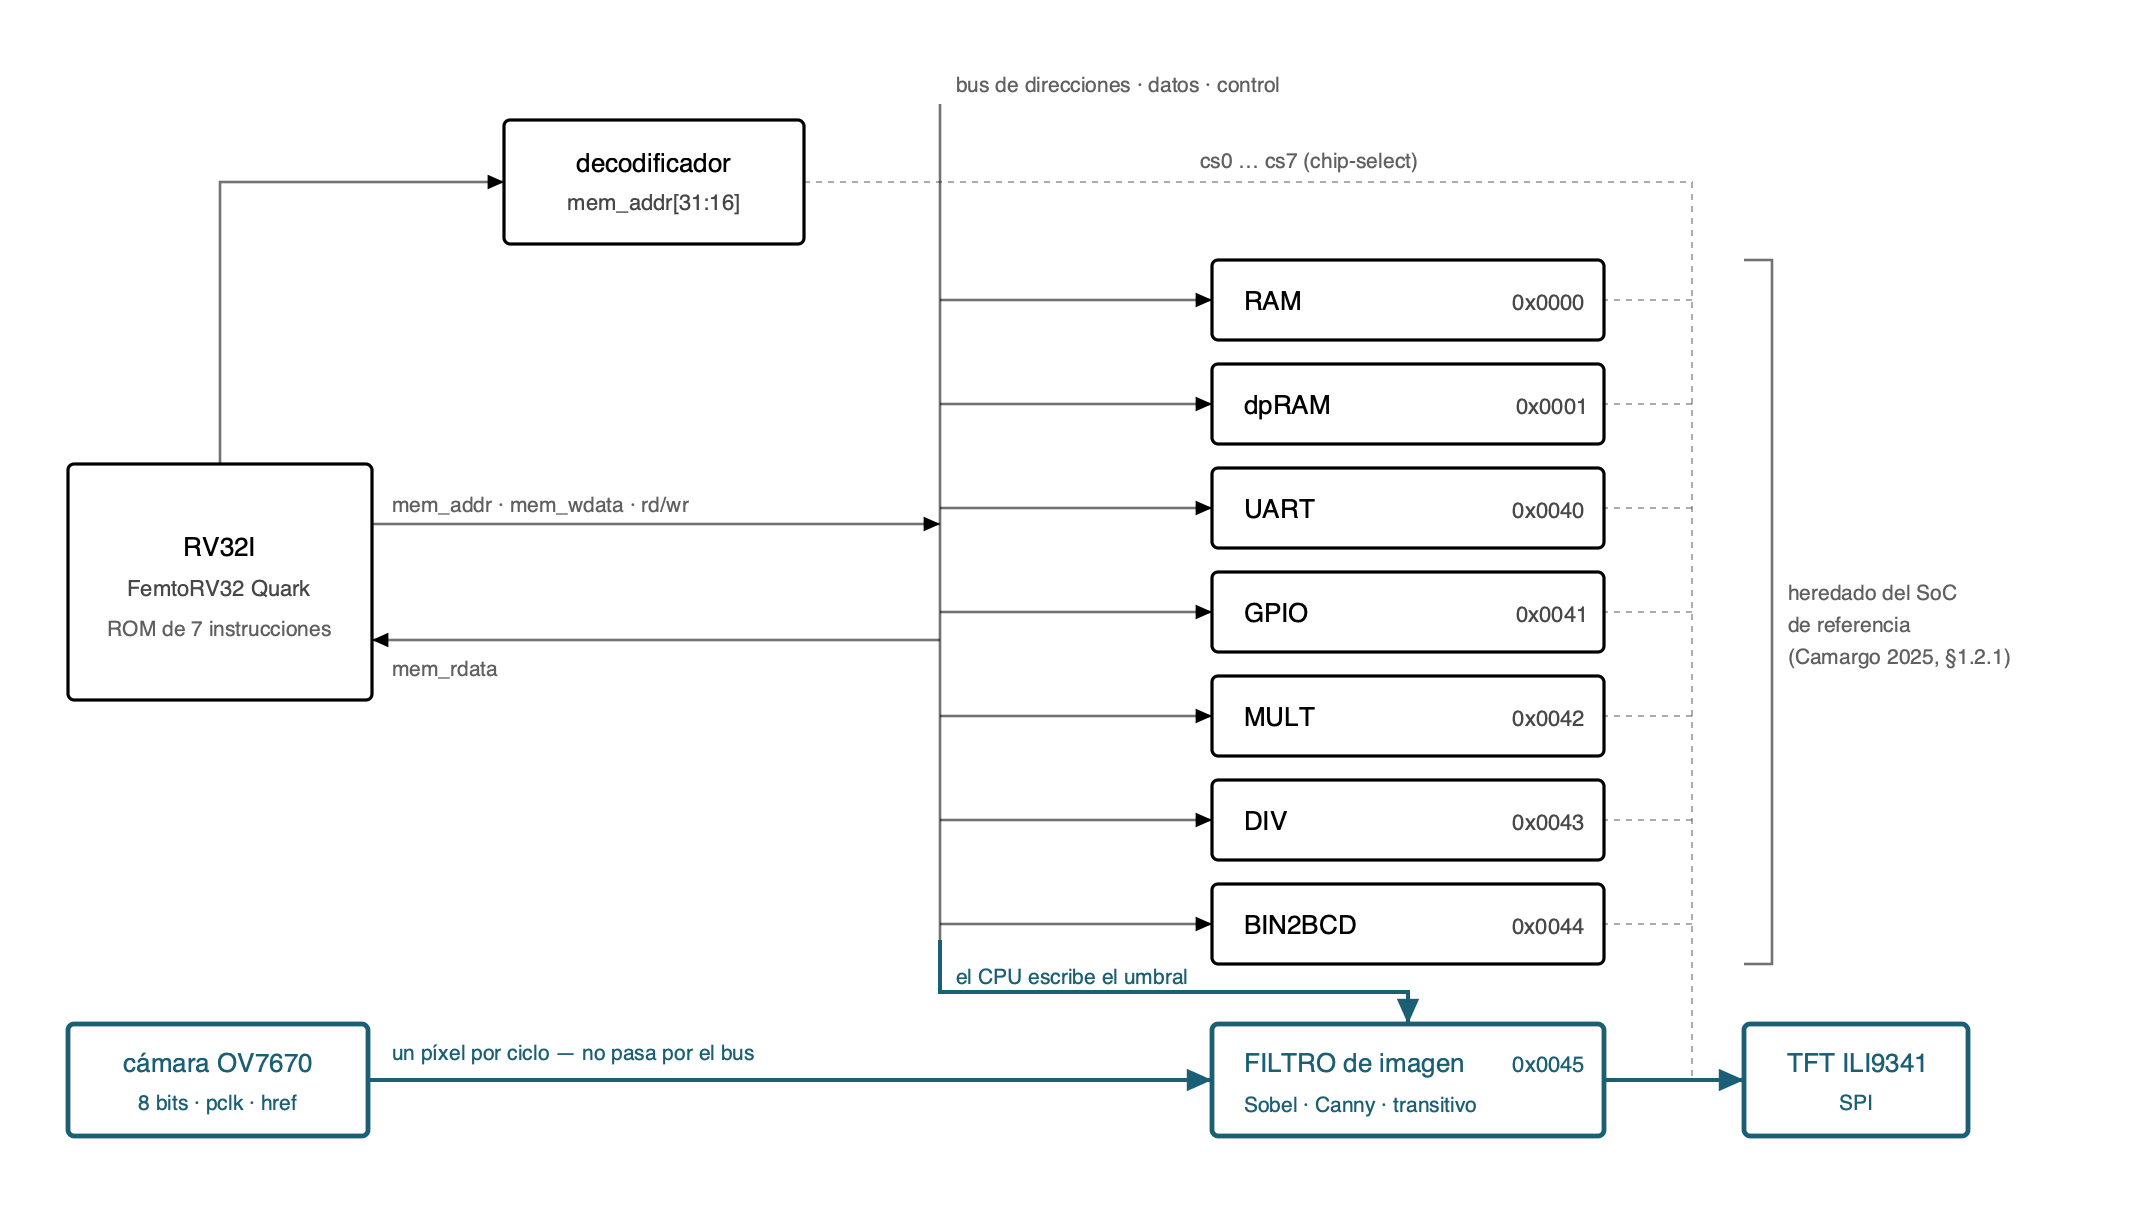
\includegraphics[keepaspectratio,alt={Figura 4.1. El sistema en silicio, en el lenguaje de bloques del SoC de referencia. Los siete periféricos en gris son los heredados; el que aparece destacado, en la base 0x0045, es la aportación de este trabajo. Obsérvese que el camino de datos de imagen no pasa por el bus: los píxeles entran de la cámara al filtro y salen de éste a la pantalla a un píxel por ciclo, y lo único que el procesador pone en el bus es el umbral.}]{figuras/fig_4_1_soc.png}}
\caption{\textbf{Figura 4.1.} El sistema en silicio, en el lenguaje de
bloques del SoC de referencia. Los siete periféricos en gris son los
heredados; el que aparece destacado, en la base \texttt{0x0045}, es la
aportación de este trabajo. Obsérvese que \textbf{el camino de datos de
imagen no pasa por el bus}: los píxeles entran de la cámara al filtro y
salen de éste a la pantalla a un píxel por ciclo, y lo único que el
procesador pone en el bus es el umbral.}
\end{figure}

La figura muestra por qué este periférico no se parece a los demás. Un
multiplicador o un divisor reciben sus operandos por el bus y devuelven
el resultado por el bus: el procesador los usa. El filtro, en cambio,
\textbf{tiene su propio camino de datos} ---de la cámara a la pantalla,
a un píxel por ciclo--- y del bus recibe únicamente un parámetro de
configuración. El procesador no lo usa: lo \textbf{ajusta}.

\begin{quote}
Esa distinción es la que el Capítulo 6 convierte en argumento. Un
periférico que procesa a través del bus está limitado por el ancho de
banda del bus; uno que procesa al margen de él, no. Es la razón de que
un sistema de visión en tiempo real pueda construirse sobre un
procesador de siete instrucciones.
\end{quote}

El firmware ocupa \textbf{siete instrucciones}: inicializa, escribe el
umbral y queda en un lazo. No es un programa modesto por limitación sino
por diseño --- el procesador existe para poder cambiar un parámetro en
tiempo de ejecución, no para procesar.

\subsection{La ROM sintetizada}\label{la-rom-sintetizada}

En una FPGA el contenido de la memoria de programa se carga con el
\emph{bitstream}. \textbf{En un ASIC no hay nada que lo cargue}: los
biestables arrancan en un estado indefinido. La memoria de programa debe
por tanto sintetizarse como lógica combinacional ---una tabla de
constantes--- y no como un arreglo inicializado.

Es el primero de los cuatro cambios obligatorios de la §4.8, y el que
más sorprende a quien llega desde FPGA, porque el código funciona
idénticamente en simulación en ambos casos.

\section{4.6 Memoria: la batalla de los
recursos}\label{memoria-la-batalla-de-los-recursos}

La iCE40UP5K ofrece tres clases de almacenamiento, y el diseño usa las
tres con criterios distintos:

\begin{longtable}[]{@{}
  >{\raggedright\arraybackslash}p{(\linewidth - 4\tabcolsep) * \real{0.3333}}
  >{\raggedright\arraybackslash}p{(\linewidth - 4\tabcolsep) * \real{0.3333}}
  >{\raggedright\arraybackslash}p{(\linewidth - 4\tabcolsep) * \real{0.3333}}@{}}
\toprule\noalign{}
\begin{minipage}[b]{\linewidth}\raggedright
Recurso
\end{minipage} & \begin{minipage}[b]{\linewidth}\raggedright
Cantidad
\end{minipage} & \begin{minipage}[b]{\linewidth}\raggedright
Uso en este trabajo
\end{minipage} \\
\midrule\noalign{}
\endhead
\bottomrule\noalign{}
\endlastfoot
Celdas lógicas & 5 280 & lógica y registros pequeños \\
Bloques de memoria (4 kbit) & 30 & \textbf{memorias de línea} de las
ventanas 3×3 \\
SPRAM (256 kbit) & 4 & \textbf{framebuffers} del filtro transitivo \\
\end{longtable}

La asignación no es libre: una memoria de línea cabe en un bloque de
memoria si el sintetizador la reconoce como tal, y no la reconoce si el
código la escribe de una forma que no encaja con el patrón esperado.
Varios de los problemas de recursos del desarrollo fueron de esa
naturaleza ---memorias que se convertían en biestables por un detalle de
escritura del RTL--- y no de tamaño real del diseño.

El caso más costoso fue un \textbf{ancho de puntero insuficiente}: un
contador de direcciones con un bit de menos del necesario direcciona la
mitad de la memoria y sobrescribe la otra, produciendo una imagen que se
ve plausible pero está mal. Como en el caso del byte de luminancia, el
error sobrevive a la inspección visual.

\begin{quote}
Este apartado es el origen del título del Capítulo 6. En la FPGA los dos
primeros recursos parecen gratuitos porque ya están en el sustrato; en
el ASIC ninguno lo es, y el mismo RTL que allí cabía holgadamente aquí
define el tamaño del dado.
\end{quote}

\section{4.7 Del RTL a la FPGA}\label{del-rtl-a-la-fpga}

El camino a la FPGA impuso sus propias decisiones.

\textbf{El intercambio entre celdas lógicas y bloques de memoria.}
Forzar más memorias de línea a bloques libera celdas pero consume
bloques, que son treinta. En varios puntos del desarrollo el diseño
estuvo limitado alternativamente por uno y por otro, y la solución
consistió en mover recursos entre ambos hasta encontrar una combinación
que cerrara.

\textbf{El bug del cerrojo.} Una asignación condicional incompleta
dentro de un bloque combinacional infiere un cerrojo en lugar de lógica.
El diseño sintetiza, ocupa recursos parecidos y funciona en simulación;
en la placa produce un comportamiento dependiente de la temporización.
La herramienta lo advierte, y la advertencia es fácil de ignorar entre
otras muchas.

\textbf{El bring-up incremental.} El sistema se puso en marcha por
etapas, cada una verificable por sí misma: parpadeo, reloj,
configuración SCCB, imagen en gris, memorias de línea, filtro, umbral,
motor, procesador. La razón es que \textbf{cada etapa es el banco de
pruebas de la siguiente}: cuando el filtro no produjo imagen, disponer
de la etapa anterior funcionando permitió decidir en un solo intento si
el problema estaba en el filtro o en la captura.

\section{4.8 Del RTL al ASIC: los cuatro cambios
obligatorios}\label{del-rtl-al-asic-los-cuatro-cambios-obligatorios}

El mismo Verilog no sirve para los dos destinos. Cuatro cosas hay que
cambiar, y ninguna de ellas produce un error de simulación ---por eso
son peligrosas.

\textbf{1. La memoria de programa debe sintetizarse.} Ya explicado en la
§4.5: en silicio no existe el \emph{bitstream} que la inicializa.

\textbf{2. Reset explícito en todos los registros de control.} En una
FPGA los biestables arrancan en el valor que el \emph{bitstream} les da;
en silicio arrancan en un estado indefinido. Toda máquina de estados
necesita una señal de reinicio explícita, y omitirla produce un circuito
que en simulación arranca correctamente y en la mesa no arranca nunca.

\textbf{3. Fuera el tri-estado interno.} El bus de datos de la cámara es
bidireccional y en FPGA se describe con alta impedancia dentro del
diseño. Un ASIC de celda estándar no dispone de eso: la señal debe
partirse en un dato y un habilitador ---\texttt{cam\_sda\_o} y
\texttt{cam\_sda\_oe}--- y el tri-estado real ocurre en el anillo de
pads.

\textbf{4. Fuera las primitivas del fabricante.} Los bloques específicos
de Lattice ---el controlador del LED RGB, entre otros--- no existen en
sky130. Se sustituyen por pines ordinarios o se eliminan.

\begin{quote}
Los cuatro cambios comparten una propiedad que conviene subrayar:
\textbf{ninguno produce un fallo visible en simulación RTL}. Un diseño
con \texttt{initial} heredado de FPGA simula perfectamente y sale de
fábrica mudo. Los dos únicos que se detectaron a tiempo durante este
trabajo aparecieron en \textbf{simulación de compuertas}, después de la
síntesis, y no antes.
\end{quote}

\chapter{5. Resultados}\label{resultados}

\section{5.1 Verificación funcional}\label{verificaciuxf3n-funcional}

\begin{quote}
\textbf{Estado:} borrador 1, escrito el 2026-09-16. Fuente: cuaderno 1,
Partes 29-35. Formato Markdown para convertir con \texttt{pandoc} a Word
o LaTeX según decida la guía de la Facultad.
\end{quote}

Antes de presentar área, frecuencia o consumo conviene establecer que
los circuitos \textbf{calculan lo que deben calcular}. Esta sección lo
hace, y distingue con cuidado dos preguntas que la literatura de
implementación mezcla con frecuencia: si el hardware coincide con su
modelo de referencia, y si el resultado es bueno. Aquí sólo se responde
la primera. La segunda pertenece a la §5.6.

\subsection{5.1.1 El criterio}\label{el-criterio}

Cada filtro se especificó primero como un programa en Python ---el
\textbf{modelo golden} descrito en la §3.2--- y sólo después se escribió
su descripción en Verilog. La verificación consiste en ejecutar ambos
sobre la misma entrada y comparar \textbf{píxel a píxel}, no en
inspeccionar visualmente la salida.

La distinción no es formal. Un mapa de bordes erróneo sigue pareciendo
un mapa de bordes, de modo que la inspección visual no distingue un
circuito correcto de uno que desplaza una fila, satura un byte o
invierte un signo. Sólo la comparación numérica lo hace.

Al comparar se admite un \textbf{desplazamiento constante} entre ambas
salidas ---la técnica de \emph{best-shift} de la §3.3--- porque la
implementación en hardware introduce una latencia de segmentación que el
modelo en software no tiene. Un desfase uniforme de \emph{k} píxeles no
es un error de cálculo sino una propiedad de la arquitectura segmentada,
y se descuenta explícitamente; cualquier diferencia que sobreviva a esa
corrección sí lo es.

\subsection{5.1.2 Resultado sobre los núcleos
aislados}\label{resultado-sobre-los-nuxfacleos-aislados}

Los tres núcleos son \textbf{idénticos bit a bit} a su modelo de
referencia. En el caso del Sobel sobre un cuadro de 60×80, la
comparación arroja \textbf{0 píxeles de diferencia sobre 4 800}, y el
resultado se sostiene para los tres filtros sobre las cinco imágenes de
prueba.

\begin{longtable}[]{@{}lrrr@{}}
\toprule\noalign{}
Núcleo & Imágenes & Píxeles comparados & Diferencias \\
\midrule\noalign{}
\endhead
\bottomrule\noalign{}
\endlastfoot
Sobel 3×3 & 5 / 5 & 4 800 por cuadro & \textbf{0} \\
Canny de un salto & 5 / 5 & 4 800 por cuadro & \textbf{0} \\
Canny transitivo & 5 / 5 & 4 800 por cuadro & \textbf{0} \\
\end{longtable}

Que la coincidencia sea exacta y no aproximada tiene una causa de
diseño: los tres filtros operan \textbf{sobre enteros y sin división}.
La magnitud del gradiente usa la norma L1,
\texttt{\textbar{}Gx\textbar{}+\textbar{}Gy\textbar{}}, en lugar de la
euclídea; los pesos del operador son potencias de dos, implementadas
como desplazamientos; y el umbral es una comparación. No hay ninguna
operación cuyo redondeo pueda diferir entre una biblioteca de punto
flotante y un circuito. \textbf{La igualdad bit a bit no es una
casualidad afortunada: es consecuencia de haber elegido una aritmética
que la permite.}

\subsection{5.1.3 Resultado sobre la cadena completa con
cámara}\label{resultado-sobre-la-cadena-completa-con-cuxe1mara}

La verificación anterior alimenta el circuito con una imagen almacenada.
La cadena real recibe en cambio un flujo de video de la cámara OV7670,
con sus bordes de línea, sus tiempos muertos y su sincronismo propio.
Medida sobre ese flujo, la concordancia entre el hardware y el modelo
es:

\begin{longtable}[]{@{}lr@{}}
\toprule\noalign{}
Cadena & Concordancia \\
\midrule\noalign{}
\endhead
\bottomrule\noalign{}
\endlastfoot
Sobel & 95 -- 100 \% \\
Canny de un salto & 88 -- 99 \% \\
Canny transitivo & 96 -- 100 \% \\
Promedio a través del SoC & \textbf{97,8 \%} \\
\end{longtable}

La degradación respecto del 100 \% de la §5.1.2 no proviene del filtro
sino del \textbf{acoplamiento con la cámara}: el muestreo del flujo, el
recorte de la ventana y el instante exacto en que empieza un cuadro
introducen diferencias de uno o dos píxeles en los bordes de la imagen.
El valor más bajo corresponde al Canny de un salto, que es también el
más sensible por construcción ---un píxel que cruza el umbral alto
propaga su decisión a sus vecinos, de modo que una diferencia aislada en
la entrada puede producir varias en la salida.

\begin{quote}
\textbf{Dos precisiones de terminología, porque el número se presta a
confusión.}

Primera: los porcentajes de esta tabla son \textbf{concordancia entre el
hardware y su propio modelo de referencia}, no exactitud del filtro.
Miden si el circuito hace lo que el programa hace, no si lo que el
programa hace es correcto o útil. Un filtro mal diseñado puede alcanzar
el 100 \% de concordancia con un modelo igualmente mal diseñado.

Segunda: la \textbf{densidad de bordes} ---la fracción de píxeles
marcados, en torno al 2 \% en las imágenes de prueba--- aparece en
varias figuras de este trabajo y \textbf{no es una medida de calidad}.
Es una propiedad de la escena y del punto de operación elegido, y su
valor «correcto» depende de para qué se vaya a usar el mapa de bordes.
La §5.6.4 muestra precisamente que mover ese punto de operación cambia
el resultado de clasificación más que cambiar de filtro.
\end{quote}

\section{5.2 Resultados en FPGA}\label{resultados-en-fpga}

\begin{quote}
\textbf{Estado:} borrador 2, 2026-09-21. Fuente: cuaderno 1, Partes
25-28 y 68-82, y los informes de \texttt{nextpnr-ice40} conservados de
las corridas del 30 de julio y del 3 de agosto de 2026.
\end{quote}

Los resultados de esta sección son de una clase distinta a los del resto
del capítulo: no provienen de un informe de herramienta sino de
\textbf{un circuito que funciona sobre una mesa}, con una cámara
apuntando a un objeto y una pantalla mostrando el resultado. Es la única
parte del trabajo donde el sistema completo existe físicamente, y por
eso condiciona lo que puede afirmarse de las demás.

\subsection{5.2.1 La plataforma}\label{la-plataforma}

La implementación física se realizó sobre una \textbf{iCE40UP5K} en
tarjeta iCESugar v1.5, con una cámara \textbf{OV7670} y una pantalla
\textbf{TFT ILI9341} por SPI. El flujo de síntesis e implementación es
enteramente abierto: \texttt{yosys} para síntesis,
\texttt{nextpnr-ice40} para emplazamiento y ruteo, \texttt{icepack} para
el \emph{bitstream}.

La elección del dispositivo no es incidental. La iCE40UP5K ofrece 5 280
celdas lógicas, 30 bloques de memoria de 4 kbit y \textbf{cuatro bloques
de SPRAM de 256 kbit} --- y son estos últimos los que hacen posible el
filtro transitivo, porque permiten alojar el cuadro completo sin
consumir lógica. Esa disponibilidad es exactamente lo que desaparece al
pasar a un ASIC sin macro de memoria, y es el origen del resultado de la
§5.4.3.

\subsection{5.2.2 Los tres filtros,
funcionando}\label{los-tres-filtros-funcionando}

\begin{longtable}[]{@{}
  >{\raggedright\arraybackslash}p{(\linewidth - 6\tabcolsep) * \real{0.2500}}
  >{\raggedright\arraybackslash}p{(\linewidth - 6\tabcolsep) * \real{0.2500}}
  >{\raggedright\arraybackslash}p{(\linewidth - 6\tabcolsep) * \real{0.2500}}
  >{\raggedright\arraybackslash}p{(\linewidth - 6\tabcolsep) * \real{0.2500}}@{}}
\toprule\noalign{}
\begin{minipage}[b]{\linewidth}\raggedright
Filtro
\end{minipage} & \begin{minipage}[b]{\linewidth}\raggedright
Arquitectura
\end{minipage} & \begin{minipage}[b]{\linewidth}\raggedright
Implementación física
\end{minipage} & \begin{minipage}[b]{\linewidth}\raggedright
Umbrales en la placa
\end{minipage} \\
\midrule\noalign{}
\endhead
\bottomrule\noalign{}
\endlastfoot
Sobel & flujo & hardware, con procesador FemtoRV32 & 90 \\
Canny de un salto & flujo & hardware, con procesador FemtoRV32 & 50 /
20 \\
Canny transitivo & \textbf{framebuffer} & hardware, motor en Verilog
\textbf{sin procesador} & 60 / 30 \\
\end{longtable}

Los tres funcionan sobre la placa con cámara y pantalla en vivo. El
transitivo produce contornos \textbf{conectados y completos} ---una
letra cerrada aparece cerrada--- frente a los bordes locales de los
otros dos, que es precisamente lo que su punto fijo debe conseguir.

\begin{figure}
\centering
\pandocbounded{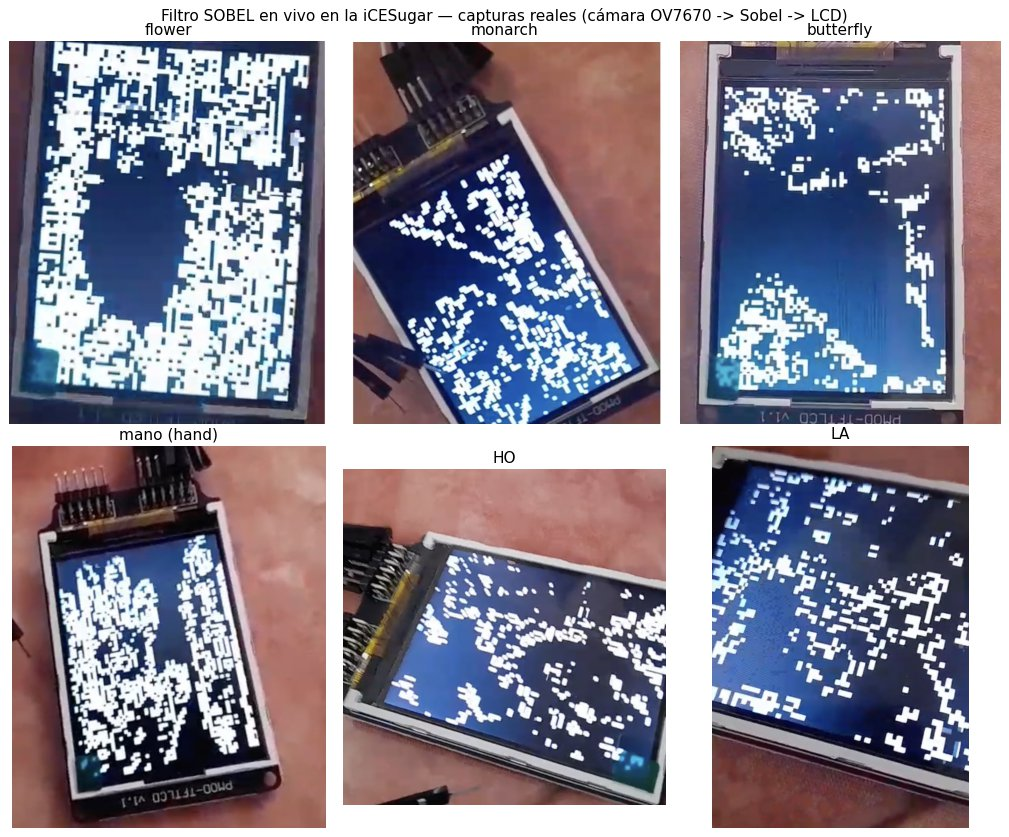
\includegraphics[keepaspectratio,alt={Figura 5.1. El filtro Sobel corriendo en vivo sobre la iCESugar, fotografiado directamente de la pantalla. Seis escenas distintas ---una flor, dos mariposas, una mano y dos letras--- recorren la cadena completa cámara → filtro → pantalla sin intervención de ningún computador. Son capturas del montaje físico, no reconstrucciones: la propia tarjeta y el cableado del módulo aparecen en el encuadre.}]{figuras/fig_5_1_sobel_en_vivo.jpg}}
\caption{\textbf{Figura 5.1.} El filtro Sobel corriendo en vivo sobre la
iCESugar, fotografiado directamente de la pantalla. Seis escenas
distintas ---una flor, dos mariposas, una mano y dos letras--- recorren
la cadena completa cámara → filtro → pantalla sin intervención de ningún
computador. Son capturas del montaje físico, no reconstrucciones: la
propia tarjeta y el cableado del módulo aparecen en el encuadre.}
\end{figure}

\subsection{5.2.3 Utilización del
dispositivo}\label{utilizaciuxf3n-del-dispositivo}

La tabla recoge el \textbf{Device utilisation} que informa
\texttt{nextpnr-ice40} tras el emplazamiento y ruteado
---\texttt{-\/-up5k\ -\/-package\ sg48}---, que es la medida
autoritativa: la que dice si el diseño entra en el dispositivo. Las
cinco filas de una misma columna proceden de \textbf{una sola corrida
con una sola versión de las herramientas}, para que sean comparables
entre sí.

\begin{longtable}[]{@{}
  >{\raggedright\arraybackslash}p{(\linewidth - 12\tabcolsep) * \real{0.1111}}
  >{\raggedleft\arraybackslash}p{(\linewidth - 12\tabcolsep) * \real{0.1481}}
  >{\raggedleft\arraybackslash}p{(\linewidth - 12\tabcolsep) * \real{0.1481}}
  >{\raggedleft\arraybackslash}p{(\linewidth - 12\tabcolsep) * \real{0.1481}}
  >{\raggedleft\arraybackslash}p{(\linewidth - 12\tabcolsep) * \real{0.1481}}
  >{\raggedleft\arraybackslash}p{(\linewidth - 12\tabcolsep) * \real{0.1481}}
  >{\raggedleft\arraybackslash}p{(\linewidth - 12\tabcolsep) * \real{0.1481}}@{}}
\toprule\noalign{}
\begin{minipage}[b]{\linewidth}\raggedright
Diseño
\end{minipage} & \begin{minipage}[b]{\linewidth}\raggedleft
LC / 5 280
\end{minipage} & \begin{minipage}[b]{\linewidth}\raggedleft
BRAM / 30
\end{minipage} & \begin{minipage}[b]{\linewidth}\raggedleft
SPRAM / 4
\end{minipage} & \begin{minipage}[b]{\linewidth}\raggedleft
E/S / 39
\end{minipage} & \begin{minipage}[b]{\linewidth}\raggedleft
\emph{f}máx sistema
\end{minipage} & \begin{minipage}[b]{\linewidth}\raggedleft
\emph{f}máx cámara
\end{minipage} \\
\midrule\noalign{}
\endhead
\bottomrule\noalign{}
\endlastfoot
Transitivo, motor dedicado \textbf{sin procesador} & 2 426 (45 \%) & 17
(56 \%) & \textbf{2 (50 \%)} & 18 (46 \%) & \textbf{28,7 MHz} ✓ & 20,6
MHz ✓ \\
SoC + Sobel & 4 848 (91 \%) & 20 (66 \%) & 0 & 18 (46 \%) & 9,5 MHz ✗ &
20,7 MHz ✓ \\
SoC + Canny de un salto & 5 234 (\textbf{99 \%}) & 24 (80 \%) & 0 & 18
(46 \%) & 9,5 MHz ✗ & 17,7 MHz ✓ \\
SoC + transitivo \textbf{por software} & 5 251 (\textbf{99 \%}) & 28 (93
\%) & 0 & 18 (46 \%) & 8,7 MHz ✗ & 20,5 MHz ✓ \\
SoC + transitivo \textbf{como periférico} & no emplaza (≈ 127 \%) & ---
& --- & --- & --- & --- \\
\end{longtable}

\begin{quote}
\textbf{Procedencia.} Las cuatro primeras filas se midieron de nuevo
para este documento. Tres de ellas ---las filas primera, tercera y
cuarta--- reprodujeron \textbf{exactamente}, celda por celda y bloque
por bloque, los informes conservados de las corridas originales de julio
y agosto de 2026. La del SoC + Sobel, cuyo informe de emplazamiento no
se había conservado, arrojó 4 848 celdas frente a las 4 878 anotadas
entonces en el cuaderno; la diferencia, de treinta celdas sobre cinco
mil, proviene de una versión distinta del sintetizador, que produce doce
tablas de consulta menos. La quinta fila no dispone de informe: el
emplazamiento no llegó a completarse, y el ≈ 127 \% es el valor
documentado en su momento.
\end{quote}

De la tabla se desprenden tres lecturas.

\textbf{La memoria grande sólo la usa un diseño.} Los cuatro bloques de
SPRAM ---256 kbit cada uno--- están sin tocar en todas las variantes de
flujo, y sólo el transitivo consume dos. Es coherente con su
arquitectura: es el único que necesita el cuadro entero a la vez. Los
filtros de flujo se las arreglan con dos filas de retardo, que caben en
los bloques de memoria pequeños.

\textbf{El límite de frecuencia lo pone el procesador, y no la
ocupación.} Los tres diseños que llevan el FemtoRV32 se agrupan entre
8,7 y 9,5 MHz mientras que el que no lo lleva alcanza 28,7 MHz:
\textbf{tres veces más rápido}. La tentación es atribuirlo a la
congestión ---los dos más lentos están al 99 \%---, pero la tabla lo
desmiente: el SoC del Sobel, \textbf{ocho puntos más vacío} que el del
Canny, cierra a la misma frecuencia, y de hecho una centésima por
debajo. La causa está en el informe de caminos críticos, que en los tres
SoC señala el mismo origen: \textbf{el registro de instrucción del
procesador}. El camino va de un flanco de subida a uno de bajada, de
modo que dispone de \textbf{medio período} en lugar de uno entero, y eso
divide por dos la frecuencia alcanzable. La síntesis lo confirma por
otra vía: los tres SoC contienen \textbf{2 048 biestables sensibles al
flanco de bajada} y el diseño sin procesador no contiene
\textbf{ninguno}. No es un problema de emplazamiento sino una propiedad
del procesador elegido, y es la razón de fondo de que las tres variantes
con CPU necesiten dividir el reloj.

\textbf{El sensor nunca fue el límite.} El dominio de la cámara cierra
con holgura en las cuatro filas medidas ---entre 17,7 y 20,7 MHz frente
a los 12 necesarios---, y es el del sistema el que falla. El cuello de
botella está del lado del procesamiento, no de la adquisición.

\begin{quote}
\textbf{Y una observación sobre el sustrato.} En los cuatro diseños el
retardo del camino crítico está dominado por el \textbf{ruteado}, que
aporta entre el 62 \% y el 72 \% del total; la lógica aporta el resto.
En una malla de interconexión fija como la de una FPGA esto es lo
esperable, y conviene tenerlo presente al leer la §5.4: en el ASIC,
donde el trazado se genera para el diseño concreto, ese reparto es otro.
\end{quote}

\subsection{5.2.4 El hallazgo de
co-diseño}\label{el-hallazgo-de-co-diseuxf1o}

El dato más importante de esta sección no es una cifra de utilización
sino una \textbf{decisión de arquitectura que la medida forzó}.

La intención inicial era que el procesador calculara la histéresis
transitiva por software, como hace en las versiones de los otros dos
filtros. Esa versión existe y funciona en simulación, con un 92,8 \% de
concordancia. Pero al intentar sintetizar el conjunto ---procesador,
memoria, framebuffers y motor--- la ocupación de celdas lógicas alcanzó
el \textbf{127 \%}: no cabía.

La respuesta fue mover el motor de histéresis de software a hardware,
como camino de datos en Verilog sin intervención del procesador. Así
implementado, la síntesis reporta \textbf{1 728 tablas de consulta} y el
emplazamiento \textbf{2 426 celdas lógicas, el 45 \% del dispositivo},
cerrando el temporizado a \textbf{28,7 MHz} con holgura.

\begin{quote}
Las dos cifras anteriores no son la misma medida, y conviene no
confundirlas: la celda lógica de la iCE40 empaqueta una tabla de
consulta \textbf{y} un biestable, de modo que un diseño con muchos
biestables sueltos ocupa más celdas que tablas tiene. Dividir el
recuento de tablas entre las 5 280 celdas del dispositivo da un 33 \%
que \textbf{subestima la ocupación real en doce puntos}. La cifra válida
es la del emplazamiento, no la de la síntesis; esta sección usa sólo la
primera.
\end{quote}

\begin{quote}
\textbf{Por qué esto es co-diseño y no una optimización.} No se trata de
que el hardware sea más rápido que el software, que es lo esperable. Se
trata de que \textbf{la restricción de recursos cambió el reparto de
responsabilidades entre las dos mitades del sistema}: la misma función,
expresada como programa, no cabía; expresada como circuito, ocupa un
tercio del dispositivo. La frontera entre lo que ejecuta el procesador y
lo que ejecuta la lógica dedicada no la fijó una preferencia de diseño
sino una medición.
\end{quote}

Este resultado reaparece transformado en la §5.4.2: en el ASIC, donde el
área no está acotada por un dispositivo fijo, el procesador vuelve a ser
viable junto al transitivo y cuesta unas nueve mil celdas. La misma
pregunta tiene respuestas opuestas en los dos sustratos.

\subsection{5.2.5 Umbrales de laboratorio y umbrales de
cámara}\label{umbrales-de-laboratorio-y-umbrales-de-cuxe1mara}

Las tres filas de la tabla anterior muestran umbrales distintos de los
que se usan en simulación. El transitivo, por ejemplo, pasó de 110/70 en
el banco de pruebas a \textbf{60/30 en la placa}.

El ajuste no es arbitrario ni es un defecto: una imagen almacenada y un
flujo de cámara tienen histogramas distintos, y el punto de operación
que extrae la estructura de una no es el que la extrae de la otra. La
§5.6.4 mide exactamente cuánto importa esa elección, y muestra que
\textbf{mover el umbral dentro de un filtro cambia el resultado de
clasificación más que cambiar de filtro}.

\begin{center}\rule{0.5\linewidth}{0.5pt}\end{center}

\begin{quote}
\textbf{Sobre la reproducibilidad de estas cifras.} Las cuatro filas
medidas se rehicieron el 21 de septiembre de 2026 con el guion
\texttt{medir\_utilizacion\_vm.sh}, que aplica a cada diseño las mismas
órdenes de lectura de fuentes que su guion de construcción original.
Tres de las cuatro reprodujeron el informe conservado sin desviarse en
una sola celda ni en un solo bloque de memoria, pese a mediar casi dos
meses entre una corrida y otra. La cuarta se desvió en treinta celdas
sobre cinco mil, y la causa está identificada: una versión distinta del
sintetizador. \textbf{El flujo es determinista a herramientas iguales},
que es lo que permite presentar estas cifras como medidas y no como
estimaciones.
\end{quote}

\section{5.3 Resultados en ASIC: los
bloques}\label{resultados-en-asic-los-bloques}

\begin{quote}
\textbf{Estado:} borrador 1, escrito el 2026-09-16. Fuente: cuaderno 1,
Partes 86-131, y el archivo de planos \texttt{ASIC\_planos/}.
\textbf{Recuento homogeneizado el 21 de septiembre de 2026.} Toda la
columna «celdas» de esta tabla son \textbf{celdas lógicas tras
emplazamiento y ruteado}, recontadas con un mismo criterio desde los
netlists archivados. Véase la §5.3.3 para cruzarlas con las de la §5.4.
\end{quote}

Esta sección presenta los circuitos que implementan \textbf{una función
cada uno}: los tres filtros por separado, los mismos con procesador, dos
bloques de interfaz y dos sistemas de visión. Son el vocabulario con el
que se construyen los sistemas de la §5.4, y su valor está en que
permiten atribuir el costo de cada pieza por separado.

Todos se llevaron a GDSII con \textbf{OpenLane} sobre el PDK abierto
\textbf{sky130A}, biblioteca \texttt{sky130\_fd\_sc\_hd}.

\subsection{5.3.1 La tabla}\label{la-tabla}

\begin{longtable}[]{@{}
  >{\raggedright\arraybackslash}p{(\linewidth - 8\tabcolsep) * \real{0.1765}}
  >{\raggedright\arraybackslash}p{(\linewidth - 8\tabcolsep) * \real{0.1765}}
  >{\raggedleft\arraybackslash}p{(\linewidth - 8\tabcolsep) * \real{0.2353}}
  >{\raggedleft\arraybackslash}p{(\linewidth - 8\tabcolsep) * \real{0.2353}}
  >{\centering\arraybackslash}p{(\linewidth - 8\tabcolsep) * \real{0.1765}}@{}}
\toprule\noalign{}
\begin{minipage}[b]{\linewidth}\raggedright
Circuito
\end{minipage} & \begin{minipage}[b]{\linewidth}\raggedright
Función
\end{minipage} & \begin{minipage}[b]{\linewidth}\raggedleft
Área del die
\end{minipage} & \begin{minipage}[b]{\linewidth}\raggedleft
Celdas
\end{minipage} & \begin{minipage}[b]{\linewidth}\centering
Signoff
\end{minipage} \\
\midrule\noalign{}
\endhead
\bottomrule\noalign{}
\endlastfoot
\texttt{sobel} & filtro Sobel 3×3 & 0,167 mm² & 5 823 & DRC/LVS/XOR =
0 \\
\texttt{canny1} & Canny de un salto, en flujo & 0,360 mm² & 12 993 &
DRC/LVS/XOR = 0 \\
\texttt{transitivo} & Canny con histéresis transitiva & 3,13 mm² & 65
659 & DRC/LVS/XOR = 0 \\
\texttt{soc\_sobel} & FemtoRV32 + Sobel & 0,37 mm² & 12 043 &
DRC/LVS/XOR = 0 \\
\texttt{soc\_canny1} & FemtoRV32 + Canny de un salto & 0,67 mm² & 22 054
& DRC/LVS/XOR = 0 \\
\texttt{soc\_trans} & FemtoRV32 + transitivo & 3,42 mm² & 72 337 &
DRC/LVS/XOR = 0 \\
\texttt{cam\_frontend} & front-end de cámara OV7670 & 0,0177 mm² & 562 &
DRC/LVS/XOR = 0 \\
\texttt{lcd\_ili9341} & driver de pantalla TFT por SPI & 0,0174 mm² &
553 & DRC/LVS/XOR = 0 \\
\texttt{vision\_top} & cámara + Sobel + framebuffer + pantalla & 1,75
mm² & 35 653 & DRC/LVS/XOR = 0 \\
\texttt{vision\_canny} & cámara + Canny + framebuffer + pantalla & 2,04
mm² & 41 925 & DRC/LVS/XOR = 0 \\
\end{longtable}

\textbf{Diez circuitos, diez veces DRC, LVS y XOR en cero.}

\subsection{5.3.2 Lo que la tabla muestra de un
vistazo}\label{lo-que-la-tabla-muestra-de-un-vistazo}

\textbf{El filtro transitivo cuesta casi veinte veces más área que el
Sobel} ---3,13 mm² contra 0,167, y once veces más celdas--- pese a
ejecutar aritmética comparable. La razón, ya anticipada, es el cuadro
completo residente: en la FPGA ese cuadro vivía en SPRAM y no consumía
lógica; aquí es un banco de biestables.

\textbf{Los dos bloques de interfaz son casi gratis.} El front-end de
cámara y el driver de pantalla ocupan menos de dieciocho milésimas de
milímetro cuadrado cada uno, alrededor de 560 celdas. Conviene tenerlo
medido porque desmonta una intuición común: el costo de un sistema de
visión embebido no está en hablar con los periféricos, está en lo que se
hace con los datos entre medias.

\begin{figure}
\centering
\pandocbounded{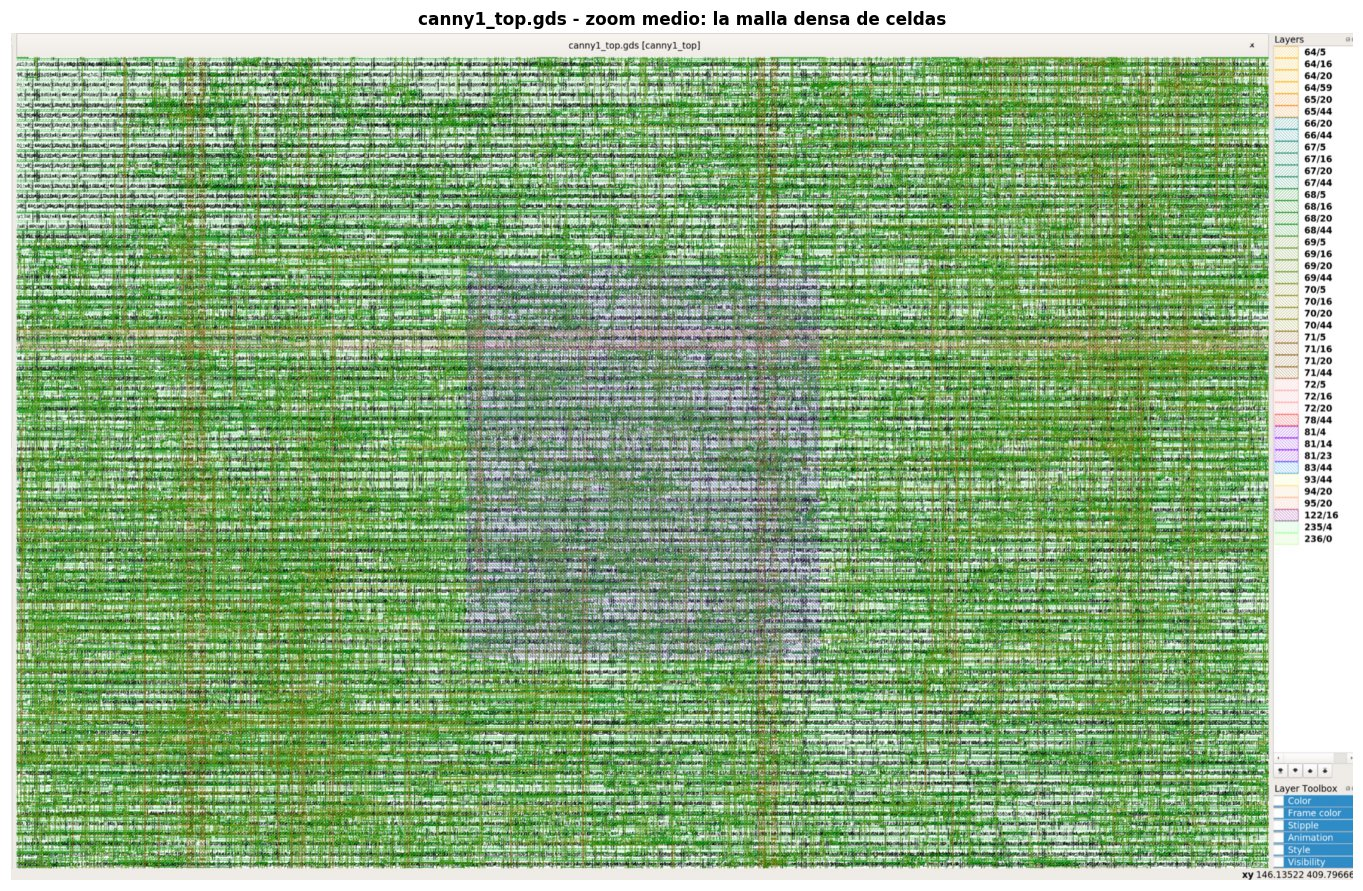
\includegraphics[keepaspectratio,alt={Figura 5.2. Acercamiento al GDSII del canny1 en KLayout. Lo que se ve no es un esquema sino el plano que iría a fábrica: filas de celdas estándar y, sobre ellas, las capas de metal que las conectan. La mancha más clara del centro es una región de menor densidad de ruteo. Las 12 993 celdas de la tabla anterior son, literalmente, estas.}]{figuras/fig_5_2_malla_canny1.jpg}}
\caption{\textbf{Figura 5.2.} Acercamiento al GDSII del \texttt{canny1}
en KLayout. Lo que se ve no es un esquema sino el plano que iría a
fábrica: filas de celdas estándar y, sobre ellas, las capas de metal que
las conectan. La mancha más clara del centro es una región de menor
densidad de ruteo. Las 12 993 celdas de la tabla anterior son,
literalmente, estas.}
\end{figure}

\textbf{Y el Sobel en silicio es mucho más rápido de lo que la FPGA
permitía.} Su camino crítico quedó en \textbf{7,69 ns} frente a un
objetivo de 20 ns, es decir que soportaría unos 130 MHz, mientras que en
la iCE40 cerraba entre 9 y 28 MHz. En silicio la lógica es rápida;
\textbf{lo caro es el área}, y ése es el eje sobre el que gira todo este
capítulo.

\subsection{5.3.3 El recuento de celdas, y cómo cruzar las dos
tablas}\label{el-recuento-de-celdas-y-cuxf3mo-cruzar-las-dos-tablas}

Esta advertencia no es un tecnicismo: afecta a cualquier comparación que
un lector intente hacer entre esta tabla y la de la §5.4.

Un circuito se puede contar en dos momentos del flujo, y las dos cifras
son legítimas:

\begin{longtable}[]{@{}
  >{\raggedright\arraybackslash}p{(\linewidth - 4\tabcolsep) * \real{0.3333}}
  >{\raggedright\arraybackslash}p{(\linewidth - 4\tabcolsep) * \real{0.3333}}
  >{\raggedright\arraybackslash}p{(\linewidth - 4\tabcolsep) * \real{0.3333}}@{}}
\toprule\noalign{}
\begin{minipage}[b]{\linewidth}\raggedright
Definición
\end{minipage} & \begin{minipage}[b]{\linewidth}\raggedright
Qué cuenta
\end{minipage} & \begin{minipage}[b]{\linewidth}\raggedright
Dónde se usa
\end{minipage} \\
\midrule\noalign{}
\endhead
\bottomrule\noalign{}
\endlastfoot
celdas de \textbf{síntesis} & el resultado de traducir el RTL a
compuertas & la tabla de la §5.4 \\
celdas \textbf{emplazadas} & lo que queda tras emplazar y rutear, con
los amortiguadores que el flujo inserta para el árbol de reloj y la
reparación de tiempos & \textbf{esta} tabla y la §5.6 \\
\end{longtable}

Durante la redacción, la columna «celdas» de este capítulo
\textbf{mezclaba las dos}, porque las fichas del cuaderno habían
registrado en cada momento el campo que la herramienta ofrecía.
\textbf{Se rehízo el recuento}: se contaron las instancias de celda
estándar directamente sobre el \textbf{netlist posterior al ruteado} de
cada circuito archivado, descartando las celdas sin función lógica
---relleno, contactos de pozo, desacoplo y diodos de antena---, con un
único criterio para los dieciséis.

El procedimiento se validó antes de aplicarlo: de los dieciséis
circuitos, \textbf{ocho reprodujeron exactamente la cifra que ya
constaba}, hasta la unidad ---los dos bloques de interfaz, los dos SoC,
los dos sistemas de visión y los dos circuitos en IHP---, que son
precisamente aquellos cuya ficha ya provenía del emplazamiento. Los ocho
restantes cambiaron, y ése era el objetivo.

\subsubsection{El factor de conversión,
medido}\label{el-factor-de-conversiuxf3n-medido}

Como en nueve circuitos se conservan las dos cifras, el paso de una a
otra no hay que estimarlo:

\begin{longtable}[]{@{}ll@{}}
\toprule\noalign{}
\endhead
\bottomrule\noalign{}
\endlastfoot
Casos medidos & 9 \\
Factor medio & \textbf{×1,21} \\
Mediana & ×1,20 \\
Rango & ×1,16 a ×1,26 \\
Desviación típica & 0,04 \\
\end{longtable}

\textbf{El emplazamiento agrega entre un 16 \% y un 26 \% de celdas},
con una dispersión estrecha. De modo que una cifra de la §5.4 se lleva a
la escala de ésta multiplicándola por 1,21, y el error de esa conversión
es de unos pocos puntos porcentuales --- no del 20 \% que separaba las
tablas antes de homogeneizarlas.

\begin{quote}
\textbf{Por qué no se convirtió también la §5.4.} Dos de sus seis
circuitos se archivaron sin netlist, de modo que convertir la tabla
habría exigido estimar dos de las seis filas. Se prefirió dejar cada
tabla \textbf{internamente homogénea} ---la §5.4 entera en celdas de
síntesis, ésta entera en celdas emplazadas--- y publicar el factor que
las relaciona, antes que producir una tabla mixta con dos filas
estimadas. Las comparaciones dentro de cada tabla son exactas; las que
cruzan de una a otra pasan por el factor.
\end{quote}

\section{5.4 Resultados en ASIC: la cadena de visión
completa}\label{resultados-en-asic-la-cadena-de-visiuxf3n-completa}

\begin{quote}
\textbf{Estado:} borrador 1, escrito el 2026-09-16. Fuente: cuaderno 1,
Partes 157-165, y la tabla maestra
\texttt{asic/tabla\_maestra/tabla\_6\_chips.py}, que la genera desde los
\texttt{metrics.csv} del flujo.
\end{quote}

La §5.3 presentó bloques: filtros solos, un front-end de cámara, un
driver de pantalla. Ésta presenta \textbf{sistemas}: seis circuitos que
llevan la cadena entera ---captura, filtrado, almacenamiento y
visualización--- en un solo dado. Los seis están organizados como una
matriz de dos variables, el \textbf{filtro} y la \textbf{presencia de
procesador}, de modo que cada comparación entre dos de ellos aísla una
sola causa.

\subsection{5.4.1 La tabla maestra}\label{la-tabla-maestra}

\begin{longtable}[]{@{}
  >{\raggedright\arraybackslash}p{(\linewidth - 20\tabcolsep) * \real{0.0811}}
  >{\raggedright\arraybackslash}p{(\linewidth - 20\tabcolsep) * \real{0.0811}}
  >{\raggedright\arraybackslash}p{(\linewidth - 20\tabcolsep) * \real{0.0811}}
  >{\centering\arraybackslash}p{(\linewidth - 20\tabcolsep) * \real{0.0811}}
  >{\raggedleft\arraybackslash}p{(\linewidth - 20\tabcolsep) * \real{0.1081}}
  >{\raggedleft\arraybackslash}p{(\linewidth - 20\tabcolsep) * \real{0.1081}}
  >{\raggedleft\arraybackslash}p{(\linewidth - 20\tabcolsep) * \real{0.1081}}
  >{\raggedleft\arraybackslash}p{(\linewidth - 20\tabcolsep) * \real{0.1081}}
  >{\centering\arraybackslash}p{(\linewidth - 20\tabcolsep) * \real{0.0811}}
  >{\centering\arraybackslash}p{(\linewidth - 20\tabcolsep) * \real{0.0811}}
  >{\centering\arraybackslash}p{(\linewidth - 20\tabcolsep) * \real{0.0811}}@{}}
\toprule\noalign{}
\begin{minipage}[b]{\linewidth}\raggedright
\#
\end{minipage} & \begin{minipage}[b]{\linewidth}\raggedright
Chip
\end{minipage} & \begin{minipage}[b]{\linewidth}\raggedright
Filtro
\end{minipage} & \begin{minipage}[b]{\linewidth}\centering
CPU
\end{minipage} & \begin{minipage}[b]{\linewidth}\raggedleft
Área (mm²)
\end{minipage} & \begin{minipage}[b]{\linewidth}\raggedleft
Celdas
\end{minipage} & \begin{minipage}[b]{\linewidth}\raggedleft
Reloj de firma
\end{minipage} & \begin{minipage}[b]{\linewidth}\raggedleft
Setup c/parásitos
\end{minipage} & \begin{minipage}[b]{\linewidth}\centering
DRC
\end{minipage} & \begin{minipage}[b]{\linewidth}\centering
LVS
\end{minipage} & \begin{minipage}[b]{\linewidth}\centering
XOR
\end{minipage} \\
\midrule\noalign{}
\endhead
\bottomrule\noalign{}
\endlastfoot
\#1 & \texttt{sobel\_completo} ᵃ & Sobel & --- & 2,45 & 36 730 & 20 ns
(50,0 MHz) & sin dato ᵇ & 0 & 0 & 0 \\
\#2 & \texttt{canny1\_completo} ᵃ & Canny1 & --- & 2,90 & 42 581 & 20 ns
(50,0 MHz) & sin dato ᵇ & 0 & 0 & 0 \\
\#3 & \texttt{trans\_completo} & Transitivo & --- & 9,61 & 137 092 & 20
ns (50,0 MHz) & \textbf{−19,35 ns} & 0 & 0 & 0 \\
\#4 & \texttt{soc\_sobel\_completo} & Sobel & ✓ & 3,03 & 46 019 & 32 ns
(31,2 MHz) & \textbf{+0,00 ns} & 0 & 0 & 0 \\
\#5 & \texttt{soc\_canny1\_completo} & Canny1 & ✓ & 3,44 & 51 037 & 36
ns (27,8 MHz) & \textbf{+0,00 ns} & 0 & 0 & 0 \\
\#6 & \texttt{soc\_trans\_completo} & Transitivo & ✓ & 10,19 & 146 216 &
36 ns (27,8 MHz) & \textbf{−18,23 ns} & 0 & 0 & 0 \\
\end{longtable}

ᵃ Estos dos se archivaron sin el directorio de reportes; sus cifras
provienen de la ficha del cuaderno y no de un \texttt{metrics.csv} del
flujo. Se marcan porque en una tabla de resultados debe poder decirse de
dónde sale cada número.

ᵇ Su ficha registra el \textbf{WNS nominal} ---0,00 ns, sin
violaciones--- pero no quedó registrado el setup ya con parásitos
extraídos, que es justamente la columna que hunde a los dos transitivos.
Se deja en blanco antes que suponer que cierran.

\textbf{Los seis llegaron a GDSII con DRC, LVS y XOR en cero.} Cuatro
cierran temporizado o carecen del dato para afirmar lo contrario; los
dos transitivos no cierran, y conviene decirlo con el número: el \#3
pediría 39,4 ns ---25,4 MHz--- y el \#6, 54,2 ns, es decir 18,4 MHz en
lugar de los 27,8 solicitados.

\begin{quote}
\textbf{Sobre el recuento de celdas, y es importante al leer junto a la
§5.3.} Las cifras de esta tabla son \textbf{celdas de síntesis}; las de
la §5.3 y la §5.6 son \textbf{celdas emplazadas}. Cada tabla es
internamente homogénea, y el paso de una escala a otra \textbf{está
medido sobre nueve circuitos que conservan las dos cifras}: el
emplazamiento agrega entre un 16 \% y un 26 \%, con un factor medio de
\textbf{×1,21} y una desviación típica de 0,04. Para comparar una cifra
de aquí con una de allá, multiplíquese por 1,21; el detalle del
procedimiento está en la §5.3.3.

Dos de los seis circuitos de esta tabla se archivaron sin
\emph{netlist}, razón por la cual no se convirtió la tabla entera: se
prefirió una tabla homogénea en su propia escala antes que una tabla
mixta con dos filas estimadas.
\end{quote}

\begin{figure}
\centering
\pandocbounded{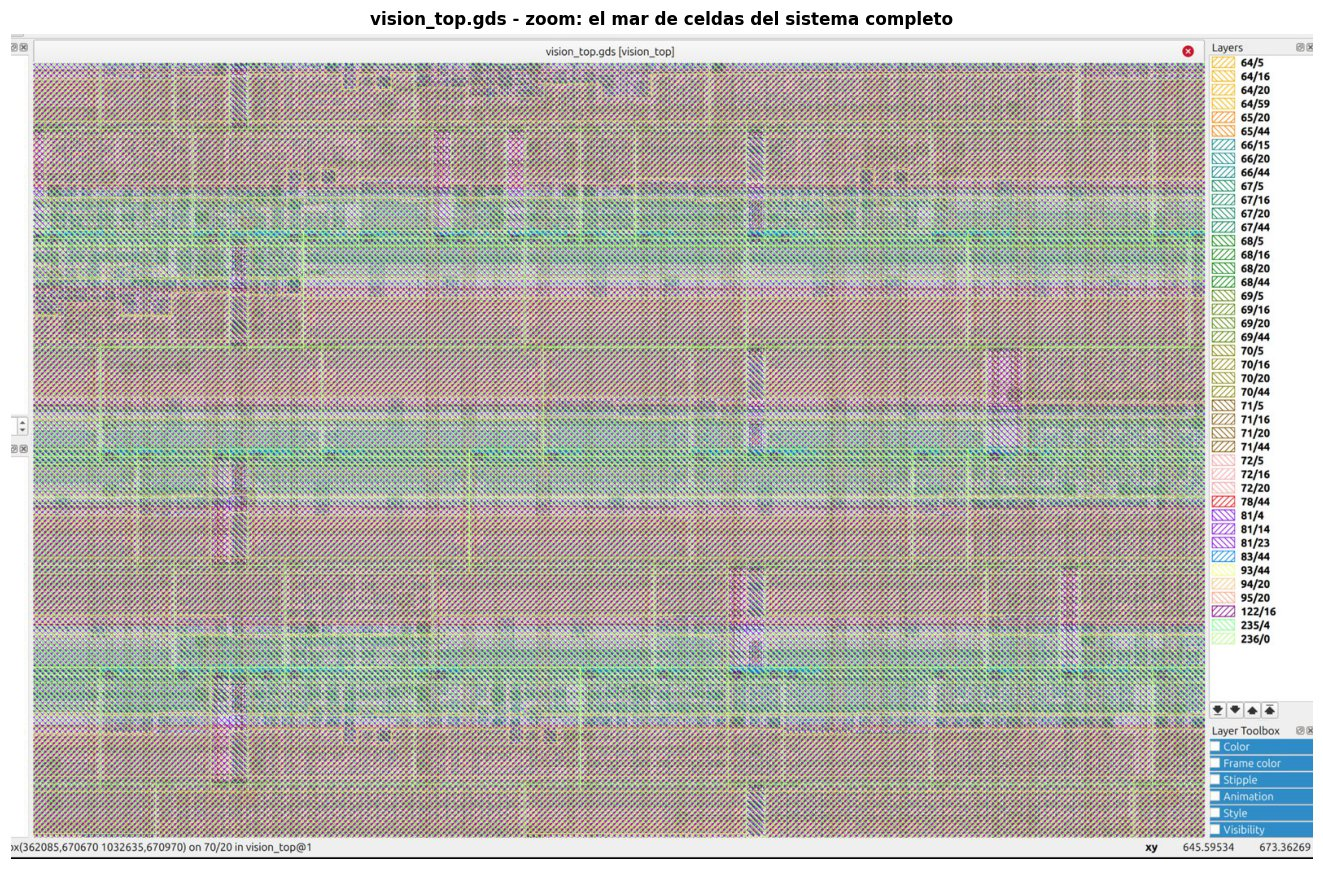
\includegraphics[keepaspectratio,alt={Figura 5.3. El mismo tipo de acercamiento, ahora sobre el sistema de visión completo. La diferencia con la figura anterior no está en la textura sino en la escala: aquí caben cámara, filtro, memoria de cuadro y controlador de pantalla en el mismo dado. Es la forma que toma en silicio la frase «el filtro es una pieza y no el circuito».}]{figuras/fig_5_3_mar_de_celdas_vision.jpg}}
\caption{\textbf{Figura 5.3.} El mismo tipo de acercamiento, ahora sobre
el sistema de visión completo. La diferencia con la figura anterior no
está en la textura sino en la escala: aquí caben cámara, filtro, memoria
de cuadro y controlador de pantalla en el mismo dado. Es la forma que
toma en silicio la frase «el filtro es una pieza y no el circuito».}
\end{figure}

\subsection{5.4.2 El procesador cuesta lo mismo, sea cual sea el
filtro}\label{el-procesador-cuesta-lo-mismo-sea-cual-sea-el-filtro}

Restando cada chip de su gemelo con procesador se obtiene el costo del
FemtoRV32, su memoria de programa y su periférico:

\begin{longtable}[]{@{}lrrrr@{}}
\toprule\noalign{}
Filtro & sin CPU & con CPU & Δ celdas & Δ relativo \\
\midrule\noalign{}
\endhead
\bottomrule\noalign{}
\endlastfoot
Sobel & 36 730 & 46 019 & \textbf{+9 289} & +25,3 \% \\
Canny de un salto & 42 581 & 51 037 & \textbf{+8 456} & +19,9 \% \\
Canny transitivo & 137 092 & 146 216 & \textbf{+9 124} & +6,7 \% \\
\end{longtable}

El incremento absoluto es \textbf{prácticamente constante}: alrededor de
nueve mil celdas, con una dispersión inferior al 5 \% entre el caso más
barato y el más caro. Es un resultado esperable ---el procesador no sabe
qué filtro tiene al lado--- pero conviene tenerlo medido, porque
convierte al procesador en un \textbf{costo fijo y presupuestable}
frente a un datapath cuyo costo varía en un factor de cuatro.

La columna relativa dice lo contrario que la absoluta, y las dos son
ciertas: el mismo procesador representa una cuarta parte del chip más
pequeño y apenas una quinceava parte del más grande. Cuál de las dos
lecturas importa depende de la pregunta. Para decidir si añadir un
procesador a un diseño dado, manda la absoluta.

\subsection{5.4.3 Lo que de verdad cuesta caro no es el cerebro: es la
memoria}\label{lo-que-de-verdad-cuesta-caro-no-es-el-cerebro-es-la-memoria}

El mismo ejercicio, hecho ahora sobre el eje del filtro en lugar del
procesador, produce el resultado central de este capítulo:

\begin{longtable}[]{@{}
  >{\raggedright\arraybackslash}p{(\linewidth - 6\tabcolsep) * \real{0.2143}}
  >{\raggedright\arraybackslash}p{(\linewidth - 6\tabcolsep) * \real{0.2143}}
  >{\raggedleft\arraybackslash}p{(\linewidth - 6\tabcolsep) * \real{0.2857}}
  >{\raggedleft\arraybackslash}p{(\linewidth - 6\tabcolsep) * \real{0.2857}}@{}}
\toprule\noalign{}
\begin{minipage}[b]{\linewidth}\raggedright
Alcance del patrón
\end{minipage} & \begin{minipage}[b]{\linewidth}\raggedright
Filtro
\end{minipage} & \begin{minipage}[b]{\linewidth}\raggedleft
Celdas (sin CPU)
\end{minipage} & \begin{minipage}[b]{\linewidth}\raggedleft
Δ respecto al anterior
\end{minipage} \\
\midrule\noalign{}
\endhead
\bottomrule\noalign{}
\endlastfoot
local, ventana 3×3 & Sobel & 36 730 & --- \\
local más un salto & Canny de un salto & 42 581 & +5 851 \\
\textbf{global, cuadro completo} & Canny transitivo & \textbf{137 092} &
\textbf{+94 511} \\
\end{longtable}

Pasar de mirar una ventana de 3×3 a mirar un salto más cuesta menos de
seis mil celdas. Pasar de ahí a \textbf{mirar el cuadro entero} cuesta
noventa y cuatro mil quinientas once.

La comparación directa es la que conviene enunciar: \textbf{un
procesador RISC-V completo, con su memoria y su periférico, pesa
aproximadamente la décima parte de lo que pesa cambiar el alcance del
patrón de local a global.} Nueve mil celdas contra noventa y cuatro mil
quinientas.

Y la razón no está en la aritmética. Los tres filtros ejecutan
esencialmente las mismas operaciones sobre cada píxel; lo que cambia es
\textbf{cuánto estado hay que sostener simultáneamente}. El Sobel y el
Canny de un salto procesan en flujo y necesitan unas pocas líneas de la
imagen ---los \emph{line-buffers} de la §4.6---, mientras que la
histéresis transitiva necesita el cuadro completo residente y accesible
en cualquier orden, porque su punto fijo puede propagar una decisión
desde cualquier píxel hacia cualquier otro. En una FPGA ese cuadro es un
bloque de memoria que ya está en el sustrato; en un ASIC sin macro de
memoria es un banco de biestables, y se paga en área, en potencia y en
frecuencia.

\begin{quote}
Éste es, en una sola cifra, el argumento que el Capítulo 6 desarrolla:
\textbf{lo que decide si un algoritmo cabe en silicio no es su
complejidad aritmética sino su huella de memoria.} Los dos transitivos
son además los dos únicos chips de la tabla que no cierran temporizado,
lo que muestra que el precio de esa memoria no se cobra sólo en
milímetros cuadrados.
\end{quote}

\subsection{5.4.4 Balance}\label{balance}

Seis circuitos, 459 675 celdas en total, \textbf{seis de seis con DRC =
LVS = XOR = 0}. Dos cierran temporizado con parásitos extraídos, dos
carecen de ese dato por haberse archivado sin reportes, y dos no cierran
y se documentan con la frecuencia que sí soportarían.

Ninguno ha sido fabricado. La §5.6.1 describe la vía por la que podrían
serlo.

\section{5.5 Rendimiento: caudal y
latencia}\label{rendimiento-caudal-y-latencia}

\begin{quote}
\textbf{Estado:} borrador 2, 2026-09-21. Fuente: cuaderno 1, Partes
154-156, y la corrida de \texttt{tb\_latencia\_final.v} del 21 de
septiembre. Todas las latencias de esta sección están \textbf{medidas en
simulación}, no estimadas --- incluida la del Canny, que hasta esta
versión provenía de una fórmula y resultó estar sobrestimada en un 20
\%.
\end{quote}

Las secciones anteriores midieron el costo de cada circuito. Ésta mide
su velocidad, y lo hace separando dos magnitudes que la palabra «rápido»
confunde: el \textbf{caudal}, o cuántos píxeles salen por segundo, y la
\textbf{latencia}, o cuánto tarda un píxel concreto desde que entra
hasta que sale.

La distinción importa porque las dos arquitecturas de este trabajo se
sitúan en extremos opuestos. Un cauce segmentado puede tener latencia
alta y caudal altísimo, porque los resultados salen uno tras otro una
vez lleno; y un motor iterativo puede terminar un cuadro entero de una
vez pero tardar milisegundos en hacerlo.

\subsection{5.5.1 Las dos arquitecturas}\label{las-dos-arquitecturas}

\begin{longtable}[]{@{}
  >{\raggedright\arraybackslash}p{(\linewidth - 4\tabcolsep) * \real{0.3333}}
  >{\raggedright\arraybackslash}p{(\linewidth - 4\tabcolsep) * \real{0.3333}}
  >{\raggedright\arraybackslash}p{(\linewidth - 4\tabcolsep) * \real{0.3333}}@{}}
\toprule\noalign{}
\begin{minipage}[b]{\linewidth}\raggedright
\end{minipage} & \begin{minipage}[b]{\linewidth}\raggedright
Flujo (Sobel, Canny de un salto)
\end{minipage} & \begin{minipage}[b]{\linewidth}\raggedright
Framebuffer (Canny transitivo)
\end{minipage} \\
\midrule\noalign{}
\endhead
\bottomrule\noalign{}
\endlastfoot
Ritmo & un píxel por ciclo, una vez lleno el cauce & barre el cuadro
\textbf{K} veces hasta el punto fijo \\
Latencia & baja --- llenar el cauce & alta --- todo el cuadro por K
barridos \\
Caudal & alto & bajo \\
\end{longtable}

La razón de la asimetría está en la §4.4: la histéresis transitiva
resuelve un \textbf{punto fijo} sobre el cuadro completo, y no puede
emitir su primer píxel definitivo hasta haber comprobado que ningún
píxel del cuadro cambia de estado.

\subsection{5.5.2 Las dos latencias, y por qué no son la
misma}\label{las-dos-latencias-y-por-quuxe9-no-son-la-misma}

La palabra «latencia» designa aquí dos magnitudes distintas, y
confundirlas produce una discrepancia de un factor treinta. Conviene
separarlas antes de dar ningún número.

\textbf{La latencia de cauce} es la profundidad de la cadena de señales
de validez: cuántos ciclos median entre el primer píxel que entra y la
primera salida marcada como válida. \textbf{La latencia hasta el primer
píxel utilizable} es otra cosa: el generador de ventana 3×3 levanta su
señal de validez \textbf{sin esperar a que sus líneas de retardo se
hayan llenado}, de modo que las primeras salidas son válidas según la
señal pero se calculan sobre el contenido inicial de los buffers. El
primer píxel del que puede uno fiarse llega mucho después.

Un banco de pruebas mide las dos sobre un flujo continuo. La primera se
obtiene contando ciclos entre el primer \texttt{in\_valid} y el primer
\texttt{out\_valid}. La segunda \textbf{no se estima con ninguna
fórmula}: las memorias de línea arrancan sin inicializar, y se busca el
último ciclo cuya salida todavía depende de ese contenido indefinido.

\begin{longtable}[]{@{}
  >{\raggedright\arraybackslash}p{(\linewidth - 8\tabcolsep) * \real{0.1579}}
  >{\raggedleft\arraybackslash}p{(\linewidth - 8\tabcolsep) * \real{0.2105}}
  >{\raggedleft\arraybackslash}p{(\linewidth - 8\tabcolsep) * \real{0.2105}}
  >{\raggedleft\arraybackslash}p{(\linewidth - 8\tabcolsep) * \real{0.2105}}
  >{\raggedleft\arraybackslash}p{(\linewidth - 8\tabcolsep) * \real{0.2105}}@{}}
\toprule\noalign{}
\begin{minipage}[b]{\linewidth}\raggedright
Filtro
\end{minipage} & \begin{minipage}[b]{\linewidth}\raggedleft
Etapas 3×3
\end{minipage} & \begin{minipage}[b]{\linewidth}\raggedleft
Latencia de cauce
\end{minipage} & \begin{minipage}[b]{\linewidth}\raggedleft
Primer píxel utilizable
\end{minipage} & \begin{minipage}[b]{\linewidth}\raggedleft
En tiempo, a su reloj
\end{minipage} \\
\midrule\noalign{}
\endhead
\bottomrule\noalign{}
\endlastfoot
Sobel & 1 & \textbf{4 ciclos} & \textbf{125 ciclos} & ≈ 0,96 µs \\
Canny de un salto & 3 & \textbf{8 ciclos} & \textbf{313 ciclos} & ≈ 2,7
µs \\
SoC + Sobel & 1 & 4 ciclos & 125 ciclos & ≈ 1,05 µs \\
SoC + Canny de un salto & 3 & 8 ciclos & 313 ciclos & ≈ 3,0 µs \\
\end{longtable}

Las dos columnas tienen explicación estructural, y no es la misma.

\textbf{La de cauce} cuenta dos ciclos por etapa de ventana: el Sobel
encadena una y el Canny tres ---suavizado, gradiente y doble umbral---,
de donde cuatro y ocho.

\textbf{La del primer píxel utilizable} la fija el llenado de las líneas
de retardo, que escala con el ancho de la imagen. Para el Sobel la
medida da \textbf{exactamente 2·(W+2) = 124 ciclos} más uno, que es lo
que cuesta tener dos filas anteriores completas. Para el Canny
\textbf{no da el triple}, como una estimación conservadora sugeriría
---6·(W+2) serían 372 ciclos---, sino 313: \textbf{las tres etapas se
llenan de forma solapada y no una después de otra}, porque cada una
empieza a recibir datos en cuanto la anterior empieza a producirlos, sin
esperar a que termine de llenarse.

\begin{quote}
Obsérvese que \textbf{la presencia del procesador no altera ninguna de
las dos}, contadas en ciclos: cuatro siguen siendo cuatro y ciento
veinticinco siguen siendo ciento veinticinco. El FemtoRV32 escribe el
umbral en un registro de configuración y no participa del camino de
datos de imagen, de modo que su única influencia es indirecta ---baja la
frecuencia máxima alcanzable, y por eso los mismos 125 ciclos tardan
1,05 µs en lugar de 0,96.
\end{quote}

\subsection{5.5.3 El número de barridos del transitivo,
medido}\label{el-nuxfamero-de-barridos-del-transitivo-medido}

El motor de histéresis transitiva repite barridos hasta que ninguno
produce cambios. Ese número, \textbf{K}, no es una constante del diseño
sino una propiedad de la imagen, de modo que estimarlo no sirve: hay que
contarlo. Un banco instrumentado cuenta las entradas al estado de
barrido y los ciclos totales hasta la señal de terminado:

\begin{longtable}[]{@{}
  >{\raggedright\arraybackslash}p{(\linewidth - 8\tabcolsep) * \real{0.1579}}
  >{\raggedleft\arraybackslash}p{(\linewidth - 8\tabcolsep) * \real{0.2105}}
  >{\raggedleft\arraybackslash}p{(\linewidth - 8\tabcolsep) * \real{0.2105}}
  >{\raggedleft\arraybackslash}p{(\linewidth - 8\tabcolsep) * \real{0.2105}}
  >{\raggedleft\arraybackslash}p{(\linewidth - 8\tabcolsep) * \real{0.2105}}@{}}
\toprule\noalign{}
\begin{minipage}[b]{\linewidth}\raggedright
Imagen de clases
\end{minipage} & \begin{minipage}[b]{\linewidth}\raggedleft
K
\end{minipage} & \begin{minipage}[b]{\linewidth}\raggedleft
Ciclos totales
\end{minipage} & \begin{minipage}[b]{\linewidth}\raggedleft
A 81 MHz
\end{minipage} & \begin{minipage}[b]{\linewidth}\raggedleft
A 106 MHz
\end{minipage} \\
\midrule\noalign{}
\endhead
\bottomrule\noalign{}
\endlastfoot
Sólo bordes fuertes & \textbf{1} & 19 772 & 243 µs & 187 µs \\
\textbf{Bordes típicos} & \textbf{2} & \textbf{24 859} & \textbf{306 µs}
& 235 µs \\
Peor caso: cadena débil de 50 px & \textbf{51} & 274 122 & 3,37 ms &
2,59 ms \\
\end{longtable}

El hallazgo es que \textbf{una imagen de bordes real converge en dos
barridos}, no en los ocho que una estimación conservadora sugeriría. La
razón es propia del Canny: los píxeles débiles forman un halo fino
alrededor de los fuertes, de modo que casi todos están a un solo salto
de un borde fuerte. El primer barrido los confirma y el segundo verifica
que ya nada cambia.

El peor caso es una \textbf{cadena débil larga}, porque la confirmación
avanza aproximadamente un salto por barrido: una cadena de cincuenta
píxeles exige cincuenta y un barridos. Conviene documentarlo como lo que
es ---una cota superior real--- y señalar a la vez que esa configuración
casi no aparece en bordes de escenas reales, donde el ruido débil
aislado se descarta y los tramos débiles conectados son cortos.

\subsection{5.5.4 La brecha}\label{la-brecha}

Reuniendo las dos medidas anteriores. La columna de latencia es la del
\textbf{primer píxel utilizable}, que es la que un sistema real debe
esperar:

\begin{longtable}[]{@{}lrrr@{}}
\toprule\noalign{}
Filtro & Reloj máximo & Caudal & Latencia \\
\midrule\noalign{}
\endhead
\bottomrule\noalign{}
\endlastfoot
Sobel & 130 MHz & ≈ 130 Mpx/s & \textbf{≈ 0,96 µs} \\
Canny de un salto & 117 MHz & ≈ 117 Mpx/s & ≈ 2,7 µs \\
SoC + Sobel & 119 MHz & ≈ 119 Mpx/s & ≈ 1,05 µs \\
SoC + Canny de un salto & 106 MHz & ≈ 106 Mpx/s & ≈ 3,0 µs \\
Transitivo & 81 MHz & ≈ 16 Mpx/s & \textbf{≈ 306 µs/cuadro} \\
SoC + transitivo & 106 MHz & ≈ 20 Mpx/s & ≈ 235 µs/cuadro \\
\end{longtable}

\textbf{La latencia separa a las dos familias por un factor de entre
ochenta y trescientos} ---dos órdenes de magnitud--- y el caudal por un
factor de seis a ocho. No es una diferencia de eficiencia de
implementación: es la consecuencia directa de que una arquitectura
decide con información local y la otra necesita el cuadro entero.

\begin{quote}
Esa brecha, junto con las noventa y cuatro mil quinientas celdas de la
§5.4.3, describe el mismo fenómeno desde dos ángulos. Ampliar el alcance
del patrón de local a global cuesta casi cien mil celdas \textbf{y}
trescientas veces más latencia. El Capítulo 6 discute cuándo ese precio
se justifica.
\end{quote}

\section{5.6 Reconocimiento de patrones: del borde al
dígito}\label{reconocimiento-de-patrones-del-borde-al-duxedgito}

\begin{quote}
\textbf{Estado:} borrador 1, escrito el 2026-09-15. Fuente: cuaderno 2
§21-§30. Formato Markdown para convertir con \texttt{pandoc} a Word o
LaTeX según decida la guía de la Facultad.
\end{quote}

Las secciones anteriores de este capítulo presentaron los resultados de
un sistema que \textbf{procesa} imágenes: detecta bordes, los almacena y
los muestra. Ésta presenta los de un sistema que las \textbf{reconoce}.
La diferencia no es de grado sino de naturaleza: la salida deja de ser
una imagen y pasa a ser una decisión ---un dígito de 0 a 9, o la
declaración explícita de no saber--- y con ello el trabajo enlaza con el
planteamiento del Capítulo 1.

Los resultados que siguen son \textbf{mediciones}, no proyecciones: un
clasificador verificado contra su modelo de referencia sobre 70 000
imágenes, validado físicamente sobre una FPGA frente a una cámara real,
e implementado en dos circuitos integrados con GDS firmado.

\subsection{5.6.1 Arquitectura del
reconocedor}\label{arquitectura-del-reconocedor}

El reconocedor reutiliza íntegramente el extractor de bordes descrito en
la §4.3 y le añade dos etapas. La cadena completa consta de cuatro
pasos, y \textbf{ninguno de ellos contiene un multiplicador en el camino
de datos de imagen}:

\begin{enumerate}
\def\labelenumi{\arabic{enumi}.}
\item
  \textbf{Extracción de bordes.} El operador Sobel 3×3 sobre una ventana
  de 28×28 píxeles. La magnitud se calcula con la norma L1,
  \texttt{\textbar{}Gx\textbar{}+\textbar{}Gy\textbar{}}, evitando la
  raíz cuadrada. La orientación se codifica como \textbf{octante}
  mediante la terna
  \texttt{⟨sgn\ Gy,\ sgn\ Gx,\ \textbar{}Gy\textbar{}\textgreater{}\textbar{}Gx\textbar{}⟩}:
  tres comparaciones en lugar de una arcotangente.
\item
  \textbf{Histograma de orientaciones por zona.} El cuadro se divide en
  cuatro cuadrantes y cada píxel de borde incrementa uno de \textbf{32
  contadores} (4 zonas × 8 octantes). Los contadores saturan en lugar de
  desbordar, de modo que una escena con exceso de bordes produce un
  valor máximo y no un valor pequeño espurio.
\item
  \textbf{Pirámide espacial.} El descriptor final consta de \textbf{40
  rasgos}: los 32 contadores más ocho correspondientes a la imagen
  completa. Estos ocho \textbf{no se cuentan: se derivan} sumando los
  cuatro cuadrantes, que constituyen una partición del cuadro. Es la
  razón por la que el circuito almacena 32 contadores y no 40, y ahorra
  ocho registros de 9 bits.
\item
  \textbf{Clasificador lineal cuantizado.} Diez clases por cuarenta
  rasgos suman \textbf{400 pesos de 4 bits con signo}, una
  multiplicación-acumulación por ciclo, seguidas de \texttt{argmax}. Los
  pesos residen en una memoria de sólo lectura combinacional: \textbf{no
  consumen un solo biestable}.
\end{enumerate}

A la decisión se le superpone una \textbf{regla de rechazo}
---clasificación con opción de rechazo, en los términos de Chow
{[}1970{]}--- que exige dos condiciones simultáneas: que el número de
bordes sea plausible y que el ganador aventaje al segundo clasificado
por un margen mínimo. Si alguna falla, el circuito responde
\textbf{NADA} en lugar de arriesgar una respuesta.

\begin{quote}
\textbf{Sobre la elección del descriptor.} La combinación de rejilla
espacial e histograma de orientaciones no es original de este trabajo:
corresponde al esquema HOG propuesto por Dalal y Triggs {[}2005{]},
sobre la receta que Lowe {[}2004{]} había establecido para SIFT,
organizada en niveles según la pirámide espacial de Lazebnik, Schmid y
Ponce {[}2006{]}. Lo que este trabajo aporta es su realización en
hardware bajo restricciones severas, con cuatro decisiones propias: el
octante sin arcotangente, el nivel 0 derivado en lugar de contado, el
voto binario en lugar de ponderado por magnitud, y la construcción del
descriptor \textbf{sin almacenar la imagen}.
\end{quote}

\subsection{5.6.2 Exactitud sobre MNIST}\label{exactitud-sobre-mnist}

Se entrenó el clasificador sobre las 60 000 imágenes de entrenamiento de
MNIST y se evaluó sobre las 10 000 de prueba, con los pesos cuantizados
a 4 bits y la regla de rechazo calibrada \textbf{exclusivamente sobre el
conjunto de entrenamiento}. Se compararon cinco configuraciones de
front-end bajo idéntico procedimiento:

\begin{longtable}[]{@{}
  >{\raggedright\arraybackslash}p{(\linewidth - 8\tabcolsep) * \real{0.1579}}
  >{\raggedleft\arraybackslash}p{(\linewidth - 8\tabcolsep) * \real{0.2105}}
  >{\raggedleft\arraybackslash}p{(\linewidth - 8\tabcolsep) * \real{0.2105}}
  >{\raggedleft\arraybackslash}p{(\linewidth - 8\tabcolsep) * \real{0.2105}}
  >{\raggedleft\arraybackslash}p{(\linewidth - 8\tabcolsep) * \real{0.2105}}@{}}
\toprule\noalign{}
\begin{minipage}[b]{\linewidth}\raggedright
front-end
\end{minipage} & \begin{minipage}[b]{\linewidth}\raggedleft
exactitud
\end{minipage} & \begin{minipage}[b]{\linewidth}\raggedleft
F1 macro
\end{minipage} & \begin{minipage}[b]{\linewidth}\raggedleft
precisión al responder
\end{minipage} & \begin{minipage}[b]{\linewidth}\raggedleft
falsos positivos
\end{minipage} \\
\midrule\noalign{}
\endhead
\bottomrule\noalign{}
\endlastfoot
Sobel & 91.04 \% & 0.910 & 98.43 \% & 98 \\
SoC + Sobel & 91.03 \% & 0.910 & 98.38 \% & 103 \\
Canny 1-salto & 92.03 \% & 0.920 & 98.66 \% & 85 \\
\textbf{SoC + Canny 1-salto} & \textbf{92.46 \%} & \textbf{0.924} &
\textbf{98.84 \%} & \textbf{73} \\
Canny transitivo & 89.76 \% & 0.897 & 97.80 \% & 139 \\
\end{longtable}

El ruido experimental del procedimiento se estimó mediante
\textbf{validación cruzada de diez pliegues disjuntos} sobre las 60 000
imágenes, obteniéndose \textbf{σ = 1.32 puntos porcentuales}. Bajo ese
criterio, \textbf{las diferencias entre los cuatro primeros front-ends
no son estadísticamente demostrables}: el margen entre el mejor y el
Sobel es de 1.42 pp, inferior a la propia σ. Únicamente el Canny
transitivo se separa del conjunto, con 2.70 pp (2.05 σ), resultado que
una prueba de Mann-Whitney sobre los pliegues confirma.

\begin{figure}
\centering
\pandocbounded{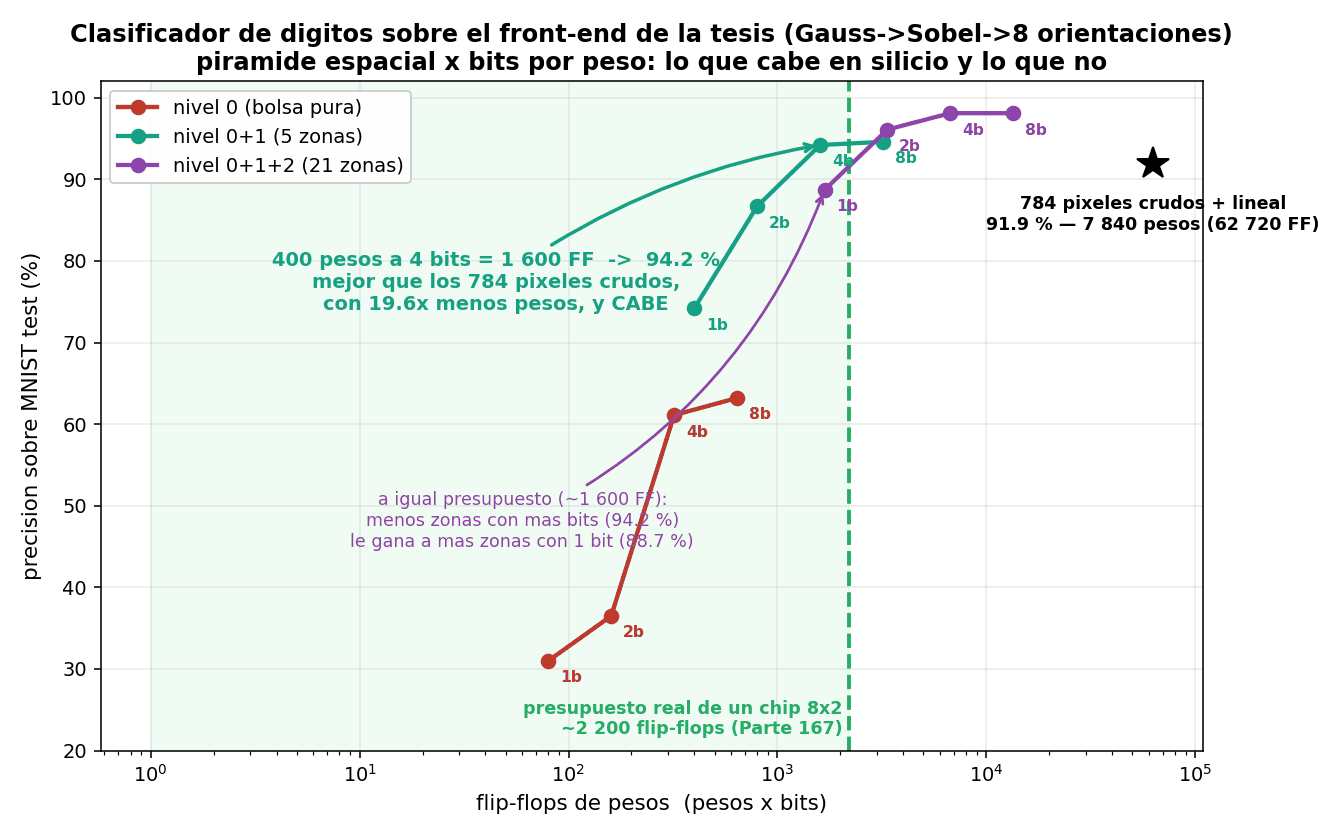
\includegraphics[keepaspectratio,alt={Figura 5.4. El espacio de diseño del clasificador, con el eje horizontal en escala logarítmica. Cada curva es un nivel de la pirámide espacial y cada punto una precisión de peso distinta. El hallazgo está en el cruce: 400 pesos de 4 bits ---1 600 biestables--- superan a los 784 píxeles crudos usando la vigésima parte de la memoria, y caben bajo el presupuesto real de un chip de 8×2 mosaicos, marcado con la línea vertical. A igualdad de memoria, la precisión de los pesos vale más que el número de zonas.}]{figuras/fig_5_4_espacio_de_diseno.png}}
\caption{\textbf{Figura 5.4.} El espacio de diseño del clasificador, con
el eje horizontal en escala logarítmica. Cada curva es un nivel de la
pirámide espacial y cada punto una precisión de peso distinta. El
hallazgo está en el cruce: \textbf{400 pesos de 4 bits ---1 600
biestables--- superan a los 784 píxeles crudos usando la vigésima parte
de la memoria}, y caben bajo el presupuesto real de un chip de 8×2
mosaicos, marcado con la línea vertical. A igualdad de memoria, la
precisión de los pesos vale más que el número de zonas.}
\end{figure}

\subsection{5.6.3 Lo que la exactitud no
muestra}\label{lo-que-la-exactitud-no-muestra}

Las medidas basadas en el \texttt{argmax} descartan la información de
los diez puntajes. Dos medidas que la conservan revelan una diferencia
que la exactitud oculta:

\begin{longtable}[]{@{}lrrr@{}}
\toprule\noalign{}
front-end & AUC macro & Brier & Brier skill \\
\midrule\noalign{}
\endhead
\bottomrule\noalign{}
\endlastfoot
SoC + Canny 1-salto & \textbf{0.9960} & \textbf{0.1465} &
\textbf{0.8371} \\
Canny 1-salto & 0.9957 & 0.1558 & 0.8268 \\
Sobel & 0.9945 & 0.1746 & 0.8059 \\
Canny transitivo & 0.9942 & \textbf{0.1991} & 0.7787 \\
SoC + Sobel & 0.9939 & 0.1749 & 0.8056 \\
\end{longtable}

El resultado de interés corresponde al Canny transitivo. En AUC ---que
mide el \textbf{ordenamiento}--- supera al SoC+Sobel; en Brier ---que
mide la \textbf{calibración}--- queda último por amplio margen.
\textbf{Ordena correctamente y decide mal.} Ello explica de forma
mecánica sus 139 falsos positivos: la reconstrucción morfológica
engruesa los contornos, el engrosamiento infla los histogramas, y el
criterio de rechazo ---que compara el mejor puntaje con el segundo---
deja hablar al circuito cuando debería callarlo.

\subsection{5.6.4 El punto de operación pesa más que el
front-end}\label{el-punto-de-operaciuxf3n-pesa-muxe1s-que-el-front-end}

Las comparaciones anteriores fijan el umbral y varían el filtro. El
experimento complementario ---fijar el filtro y \textbf{barrer el
umbral}--- arroja el resultado de mayor consecuencia práctica de esta
sección:

\begin{longtable}[]{@{}lrr@{}}
\toprule\noalign{}
magnitud & rango de exactitud & en unidades de σ \\
\midrule\noalign{}
\endhead
\bottomrule\noalign{}
\endlastfoot
el umbral, dentro del Sobel & \textbf{5.79 pp} & \textbf{4.4 σ} \\
el umbral, dentro del Canny & 0.90 pp & 0.7 σ \\
el filtro, cada uno en su óptimo & 0.38 pp & 0.3 σ \\
\end{longtable}

\textbf{Mover el umbral dentro del Sobel altera el resultado quince
veces más que cambiar de filtro.} Y la asimetría entre ambos front-ends
es el hallazgo: el Sobel presenta un óptimo estrecho ---su exactitud
recorre casi seis puntos a lo largo del rango útil--- mientras que el
Canny se mantiene en una meseta de nueve décimas. \textbf{El Canny en su
peor umbral supera al Sobel en diez de los once umbrales ensayados.}

El mecanismo reside en el algoritmo: el Sobel aplica un corte único y
nada recupera al píxel que queda por debajo; el Canny dispone de dos
umbrales y una histéresis que promueve el píxel débil adyacente a uno
fuerte. \textbf{La histéresis es un mecanismo de recuperación}, y de ahí
su insensibilidad.

\begin{quote}
\textbf{Consecuencia de diseño.} El front-end y el registro escribible
resuelven el mismo problema por vías distintas: el Canny adquiere
\textbf{en hardware} ---un \emph{line-buffer} adicional y ocho
comparaciones--- buena parte de la robustez que el Sobel obtiene
mediante \textbf{un procesador} capaz de reescribir el umbral. No son
decisiones que se sumen: son, en buena medida, \textbf{alternativas}.
\end{quote}

\subsection{5.6.5 El RTL contra el modelo, sobre el conjunto
completo}\label{el-rtl-contra-el-modelo-sobre-el-conjunto-completo}

Las cifras anteriores son del modelo en Python. La pregunta que decide
si sirven de algo es si el circuito las reproduce, y se respondió por el
camino más exigente disponible: \textbf{ejecutar el RTL sobre las diez
mil imágenes de prueba} en el simulador y comparar, no los porcentajes
agregados, sino cada predicción con la del modelo.

\begin{longtable}[]{@{}
  >{\raggedright\arraybackslash}p{(\linewidth - 2\tabcolsep) * \real{0.5000}}
  >{\raggedright\arraybackslash}p{(\linewidth - 2\tabcolsep) * \real{0.5000}}@{}}
\toprule\noalign{}
\begin{minipage}[b]{\linewidth}\raggedright
Comparación
\end{minipage} & \begin{minipage}[b]{\linewidth}\raggedright
Resultado
\end{minipage} \\
\midrule\noalign{}
\endhead
\bottomrule\noalign{}
\endlastfoot
Predicciones idénticas & \textbf{10 000 / 10 000} \\
Exactitud del RTL / del modelo & \textbf{91.04 \% / 91.04 \%} \\
Matriz de confusión & idéntica elemento por elemento \\
Veredictos de la clase de rechazo & \textbf{10 000 / 10 000}
idénticos \\
Cuadros aceptados · precisión al responder & 8 838 (88.38 \%) · 95.44
\%, en ambos \\
\end{longtable}

\begin{figure}
\centering
\pandocbounded{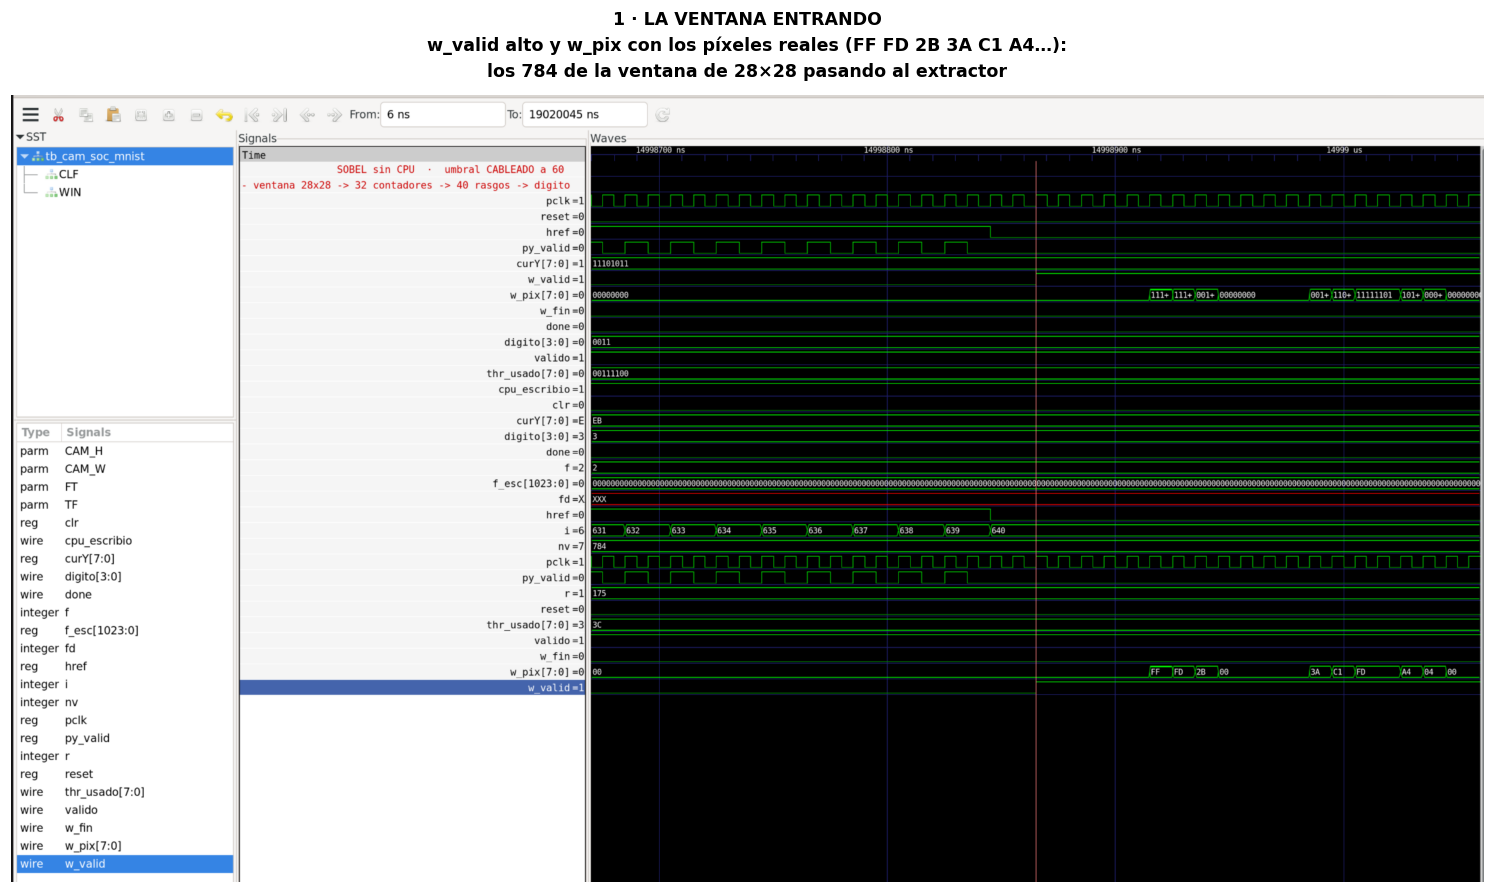
\includegraphics[keepaspectratio,alt={Figura 5.5. La ventana de 28×28 entrando al extractor, vista en el simulador. La señal w\_valid marca cada píxel válido y w\_pix lleva su valor ---FF FD 2B 3A C1 A4\ldots---; los 784 de la ventana pasan uno a uno antes de que done presente un dígito. Es el nivel al que se hizo la comparación contra el modelo: no se compararon porcentajes, se compararon señales.}]{figuras/fig_5_5_ventana_al_extractor.png}}
\caption{\textbf{Figura 5.5.} La ventana de 28×28 entrando al extractor,
vista en el simulador. La señal \texttt{w\_valid} marca cada píxel
válido y \texttt{w\_pix} lleva su valor
---\texttt{FF\ FD\ 2B\ 3A\ C1\ A4}\ldots---; los 784 de la ventana pasan
uno a uno antes de que \texttt{done} presente un dígito. Es el nivel al
que se hizo la comparación contra el modelo: no se compararon
porcentajes, se compararon señales.}
\end{figure}

No son cifras «parecidas» ni «dentro del margen de error»: \textbf{las
diez mil predicciones y los diez mil veredictos coinciden uno por uno},
y la matriz de confusión es la misma casilla por casilla. La
verificación de los filtros de la §5.1 se hizo sobre cinco imágenes;
ésta se hizo sobre diez mil, e incluye la decisión de rechazo, que es
lógica de comparación y no de aritmética.

\begin{quote}
Conviene precisar el alcance, porque más adelante aparece una cifra
distinta. Lo que aquí es exacto es el \textbf{clasificador completo}
---descriptor, pesos y decisión--- evaluado imagen por imagen. El 99.91
\% que informa la §5.6.6 se refiere a otra comparación: la del
\textbf{extractor de bordes} píxel a píxel dentro de la cadena, cuyas
discrepancias se concentran en la última fila del cuadro y no alteran
ninguna de las diez mil clasificaciones. Son dos medidas de objetos
distintos y no se contradicen.
\end{quote}

\subsection{5.6.6 Validación física}\label{validaciuxf3n-fuxedsica}

La validación sobre la placa se realizó en dos ensayos distintos, que
miden cosas distintas y cuyos resultados no deben confundirse.

\begin{figure}
\centering
\pandocbounded{
\includegraphics[keepaspectratio,alt={Figura 5.6. La cadena completa ---cámara, procesador, filtro y clasificador--- en señales, sobre la escena del dígito 3. El panel A muestra los 19 ms de dos cuadros: el veredicto sale en el primero y no cambia en el segundo. El panel B captura el instante en que el procesador sustituye el umbral por omisión del RTL, 110, por el 90 que escribe el firmware, con el camino de datos todavía en reinicio. El panel C mide los 639,5 µs que tardan las 400 multiplicaciones-acumulaciones y el argmax.}]{figuras/fig_5_6_cadena_en_senales.png}}
\caption{\textbf{Figura 5.6.} La cadena completa ---cámara, procesador,
filtro y clasificador--- en señales, sobre la escena del dígito 3. El
panel A muestra los 19 ms de dos cuadros: el veredicto sale en el
primero y no cambia en el segundo. El panel B captura el instante en que
\textbf{el procesador sustituye el umbral por omisión del RTL, 110, por
el 90 que escribe el firmware}, con el camino de datos todavía en
reinicio. El panel C mide los 639,5 µs que tardan las 400
multiplicaciones-acumulaciones y el \texttt{argmax}.}
\end{figure}

\textbf{Primer ensayo: diez dígitos grabados en el propio bitstream.} Se
embebieron diez imágenes de MNIST en la memoria de configuración y se
hizo que el circuito informara sus veredictos por el puerto serie, sin
cámara. La placa acertó \textbf{ocho de los diez}, y lo relevante no son
los ocho aciertos sino los dos fallos: el circuito confunde el
\textbf{2} con un 0 y el \textbf{3} con un 8, \textbf{exactamente los
mismos dos dígitos y exactamente las mismas respuestas equivocadas} que
había dado la simulación del diseño completo. Ninguno de los diez cambió
de respuesta a lo largo de unas treinta repeticiones.

\begin{quote}
Reproducir un acierto puede ser casualidad; reproducir un error
específico y repetido, no. Este ensayo no mide la exactitud del sistema
---diez imágenes no son una medida estadística--- sino que
\textbf{cierra el último eslabón de la traducción}: el diseño
sintetizado, emplazado, ruteado y cargado en silicio se comporta como el
RTL verificado, errores incluidos.
\end{quote}

\begin{figure}
\centering
\pandocbounded{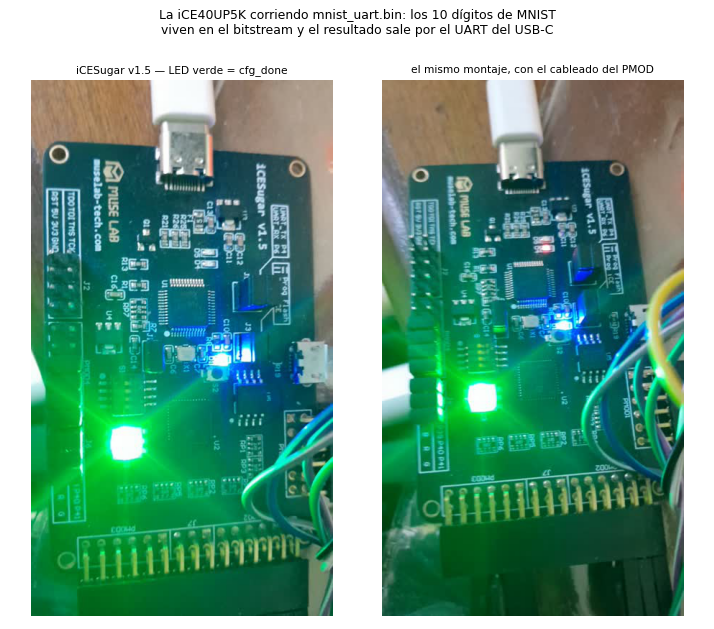
\includegraphics[keepaspectratio,alt={Figura 5.7. La tarjeta durante ese primer ensayo, con el mapa de bits cargado. El diodo verde está cableado a la señal de configuración terminada; el azul parpadea con el latido del sistema. Los diez veredictos salen por el puerto serie del mismo conector que alimenta la tarjeta. A la derecha, el mismo montaje con el cableado del módulo de pantalla ya conectado.}]{figuras/fig_5_7_la_placa_uart.png}}
\caption{\textbf{Figura 5.7.} La tarjeta durante ese primer ensayo, con
el mapa de bits cargado. El diodo verde está cableado a la señal de
configuración terminada; el azul parpadea con el latido del sistema. Los
diez veredictos salen por el puerto serie del mismo conector que
alimenta la tarjeta. A la derecha, el mismo montaje con el cableado del
módulo de pantalla ya conectado.}
\end{figure}

\textbf{Segundo ensayo: dígitos manuscritos ante la cámara.} El sistema
completo ---procesador RISC-V, periférico de umbrales, front-end Canny y
clasificador--- se enfrentó a dígitos escritos a mano y captados por una
cámara OV7670. \textbf{El circuito reconoció nueve de diez dígitos},
coincidiendo exactamente con lo que la simulación había predicho para
esa configuración.

Ese acuerdo, sin embargo, no se obtuvo al primer intento, y la causa
merece registrarse porque es la única discrepancia entre simulación y
silicio de todo el trabajo. En la primera versión la placa respondía
\textbf{ocho de diez} mientras la simulación sostenía nueve. El umbral
inferior del front-end se leía desde el módulo de control mediante una
\textbf{referencia jerárquica} ---\texttt{SOC.flt\_tlo}--- en lugar de
un puerto declarado. Ambas herramientas aceptaron el archivo sin una
sola advertencia y construyeron circuitos distintos: \texttt{iverilog}
resuelve la referencia y simula con el umbral escrito por el procesador,
mientras que el sintetizador crea un cable implícito de un bit que nadie
gobierna y fija el umbral inferior en cero. Sustituida la referencia por
un \textbf{puerto real}, la placa pasó a nueve de diez: el valor que la
simulación predecía.

\begin{quote}
\textbf{La lección no es que hubiera un error, sino dónde estaba.} El
RTL era legal, la simulación era correcta y la síntesis también lo era;
lo que falló fue suponer que ambas leían la misma descripción. Una
construcción que el lenguaje admite y que las dos herramientas
interpretan de forma distinta es indetectable por inspección y
silenciosa en los registros de ambas. Se deja escrita la regla de
trabajo que se adoptó a partir de aquí: \textbf{toda señal que cruce una
frontera de módulo se declara como puerto}, aunque el simulador acepte
el atajo.
\end{quote}

La verificación del extractor contra su modelo de referencia arrojó
\textbf{99.91 \%} de coincidencia exacta píxel a píxel para el Sobel y
\textbf{99.93 \%} para el Canny, concentrándose las diferencias en la
última fila del cuadro.

\subsection{5.6.7 Implementación en
silicio}\label{implementaciuxf3n-en-silicio}

El reconocedor se llevó a tecnología \texttt{sky130\_fd\_sc\_hd} en dos
variantes, ejecutando el flujo completo de OpenLane hasta la firma del
GDS:

\begin{longtable}[]{@{}lrr@{}}
\toprule\noalign{}
magnitud & Sobel & Canny 1-salto \\
\midrule\noalign{}
\endhead
\bottomrule\noalign{}
\endlastfoot
área del \emph{die} & 0.845 mm² & 0.890 mm² \\
celdas tras síntesis & 16 718 & 17 373 \\
celdas emplazadas & 19 949 & 20 921 \\
período de reloj & 30 ns (33.3 MHz) & 30 ns (33.3 MHz) \\
holgura con parásitos (\texttt{spef\_wns}) & \textbf{0.00 ns} &
\textbf{0.00 ns} \\
DRC · LVS · XOR & 0 · 0 · 0 & 0 · 0 · 0 \\
\end{longtable}

Ambos circuitos cierran el temporizado con los parásitos del
interconexionado extraídos y superan las tres verificaciones de firma
sin observaciones. Merece señalarse que \textbf{cierran más rápido que
los circuitos de visión equivalentes} ---que requirieron 32 y 36 ns---,
lo que resulta coherente con la ausencia de memoria de cuadro: es el
multiplexor de lectura del \emph{framebuffer} el que constituye el
camino crítico de aquéllos.

\textbf{Son los primeros circuitos de este trabajo cuya salida no es una
imagen.} Los diez presentados en las secciones §5.3 y §5.4 procesan;
éstos reconocen.

\subsection{5.6.8 El costo relativo del front-end depende del
sistema}\label{el-costo-relativo-del-front-end-depende-del-sistema}

La comparación de área entre ambos front-ends admite cuatro niveles de
integración. Las cuatro filas están en \textbf{celdas emplazadas}, la
misma escala de la §5.3, de modo que los cocientes son directamente
comparables entre sí:

\begin{longtable}[]{@{}
  >{\raggedright\arraybackslash}p{(\linewidth - 6\tabcolsep) * \real{0.2000}}
  >{\raggedleft\arraybackslash}p{(\linewidth - 6\tabcolsep) * \real{0.2667}}
  >{\raggedleft\arraybackslash}p{(\linewidth - 6\tabcolsep) * \real{0.2667}}
  >{\raggedleft\arraybackslash}p{(\linewidth - 6\tabcolsep) * \real{0.2667}}@{}}
\toprule\noalign{}
\begin{minipage}[b]{\linewidth}\raggedright
nivel
\end{minipage} & \begin{minipage}[b]{\linewidth}\raggedleft
Sobel
\end{minipage} & \begin{minipage}[b]{\linewidth}\raggedleft
Canny
\end{minipage} & \begin{minipage}[b]{\linewidth}\raggedleft
factor
\end{minipage} \\
\midrule\noalign{}
\endhead
\bottomrule\noalign{}
\endlastfoot
filtro aislado & 5 823 & 12 993 & \textbf{2.23×} \\
con procesador & 12 043 & 22 054 & 1.83× \\
sistema de visión completo & 35 653 & 41 925 & 1.18× \\
reconocedor con procesador & 19 949 & 20 921 & 1.05× \\
\textbf{reconocedor que además muestra} & \textbf{38 643} & \textbf{39
794} & \textbf{1.03×} \\
\end{longtable}

\textbf{El sobrecosto del Canny se diluye conforme crece el sistema que
lo rodea.} Considerado de forma aislada cuesta un \textbf{123 \%} más;
con un procesador al lado, un 83 \%; dentro de un sistema de visión, un
18 \%; integrado en un reconocedor, un 5 \%; y en un reconocedor que
además dibuja en pantalla, un \textbf{3 \%}. El motivo es que el
clasificador ---histograma, pirámide y 400 multiplicaciones--- es
idéntico en ambas variantes y domina el área, mientras que la diferencia
se reduce al tercer \emph{line-buffer}.

De ello se sigue una conclusión condicional: \textbf{el Sobel aventaja
al Canny en área únicamente cuando el filtro constituye el circuito
completo.} En un sistema que reconoce, esa ventaja ---la única que el
Sobel conserva, según §5.6.2 a §5.6.4--- deja de ser determinante.

\begin{center}\rule{0.5\linewidth}{0.5pt}\end{center}

\subsection{Referencias de la
sección}\label{referencias-de-la-secciuxf3n}

\begin{itemize}
\tightlist
\item
  Chow, C. K. (1970). \emph{On Optimum Recognition Error and Reject
  Tradeoff.} IEEE Trans. Inf. Theory, 16(1), 41-46.
\item
  Dalal, N. y Triggs, B. (2005). \emph{Histograms of Oriented Gradients
  for Human Detection.} CVPR, 886-893.
\item
  Lazebnik, S., Schmid, C. y Ponce, J. (2006). \emph{Beyond Bags of
  Features: Spatial Pyramid Matching.} CVPR, 2169-2178.
\item
  Lowe, D. G. (2004). \emph{Distinctive Image Features from
  Scale-Invariant Keypoints.} IJCV, 60(2), 91-110.
\end{itemize}

\section{5.7 Verificación eléctrica del camino
crítico}\label{verificaciuxf3n-eluxe9ctrica-del-camino-cruxedtico}

\begin{quote}
\textbf{Estado:} borrador 1, 2026-09-21. Fuente: cuaderno 2, §33. Todas
las cifras de esta sección proceden de corridas de NGSpice sobre
\texttt{sky130\_fd\_sc\_hd} en la esquina típica, 1,8 V y 25 °C, y de
los ficheros de parásitos extraídos de los dos reconocedores.
\end{quote}

Las secciones anteriores aceptaron sin discusión lo que el analizador de
tiempos informa. Ésta pregunta si ese número es correcto, y lo hace por
el único camino que no depende de la misma herramienta: \textbf{resolver
los transistores}.

La pregunta no es ociosa. Un analizador estático no simula: consulta
tablas caracterizadas de antemano e interpola. Es rapidísimo y es lo que
permite firmar un circuito de doscientas mil instancias, pero entre su
respuesta y la física median un modelo de celda, un modelo de cable y un
procedimiento de interpolación. Comprobar cuánto de lo que informa
sobrevive a una simulación eléctrica es, por tanto, una verificación del
instrumento y no del circuito.

\subsection{5.7.1 Por qué el camino crítico y no el
chip}\label{por-quuxe9-el-camino-cruxedtico-y-no-el-chip}

Simular los dos reconocedores enteros no es inviable por tamaño
---\texttt{pan\_sobel} tiene 116 314 transistores y en este trabajo ya
se simuló un procesador de 121 310--- sino \textbf{por tiempo}: para que
el clasificador vea sus 784 píxeles hay que hacerle entrar un cuadro
completo, y eso son 633 800 ciclos, unos treinta y dos veces más
actividad que la simulación de procesador ya realizada.

El camino crítico, en cambio, son \textbf{treinta y siete celdas} en un
chip y treinta y seis en el otro. Se extrajeron del reporte del
analizador, se reconstruyeron como cadena aislada con la carga y la
pendiente que el propio reporte declara en cada etapa, y se resolvieron
en NGSpice.

\subsection{5.7.2 El resultado}\label{el-resultado}

Se aplicaron cinco variantes del mismo banco, cada una añadiendo un
ingrediente al anterior, de modo que la diferencia entre dos renglones
consecutivos aísla la contribución de ese ingrediente:

\begin{longtable}[]{@{}
  >{\raggedright\arraybackslash}p{(\linewidth - 4\tabcolsep) * \real{0.2727}}
  >{\raggedleft\arraybackslash}p{(\linewidth - 4\tabcolsep) * \real{0.3636}}
  >{\raggedleft\arraybackslash}p{(\linewidth - 4\tabcolsep) * \real{0.3636}}@{}}
\toprule\noalign{}
\begin{minipage}[b]{\linewidth}\raggedright
\end{minipage} & \begin{minipage}[b]{\linewidth}\raggedleft
\texttt{pan\_sobel} (37 etapas)
\end{minipage} & \begin{minipage}[b]{\linewidth}\raggedleft
\texttt{pan\_canny} (36 etapas)
\end{minipage} \\
\midrule\noalign{}
\endhead
\bottomrule\noalign{}
\endlastfoot
\textbf{Analizador estático, con parásitos} & \textbf{12,230 ns} &
\textbf{9,890 ns} \\
A · las puertas solas & 4,646 ns & 4,424 ns \\
B · más la capacitancia extraída, agrupada & 8,159 ns & 7,552 ns \\
C · más la pendiente de entrada real & 8,178 ns & 7,588 ns \\
D0 · más la topología del fichero de parásitos, \textbf{con R = 0} &
7,603 ns & 7,022 ns \\
D · más la \textbf{resistencia medida} de cada tramo & 7,620 ns & 7,043
ns \\
E · más la \textbf{celda extraída del \emph{layout}} & \textbf{9,694 ns}
& \textbf{8,962 ns} \\
\emph{fracción del retardo que la simulación reproduce} & \emph{79,3 \%}
& \emph{90,6 \%} \\
\end{longtable}

La variante \textbf{D0 es un control}, idéntica a la D salvo en que sus
resistencias valen cero. Sin ella, el efecto de la resistencia y el de
\emph{repartir} la capacitancia a lo largo del árbol en vez de agruparla
en un nodo quedarían sumados en una sola cifra y no podrían separarse.

\begin{figure}
\centering
\pandocbounded{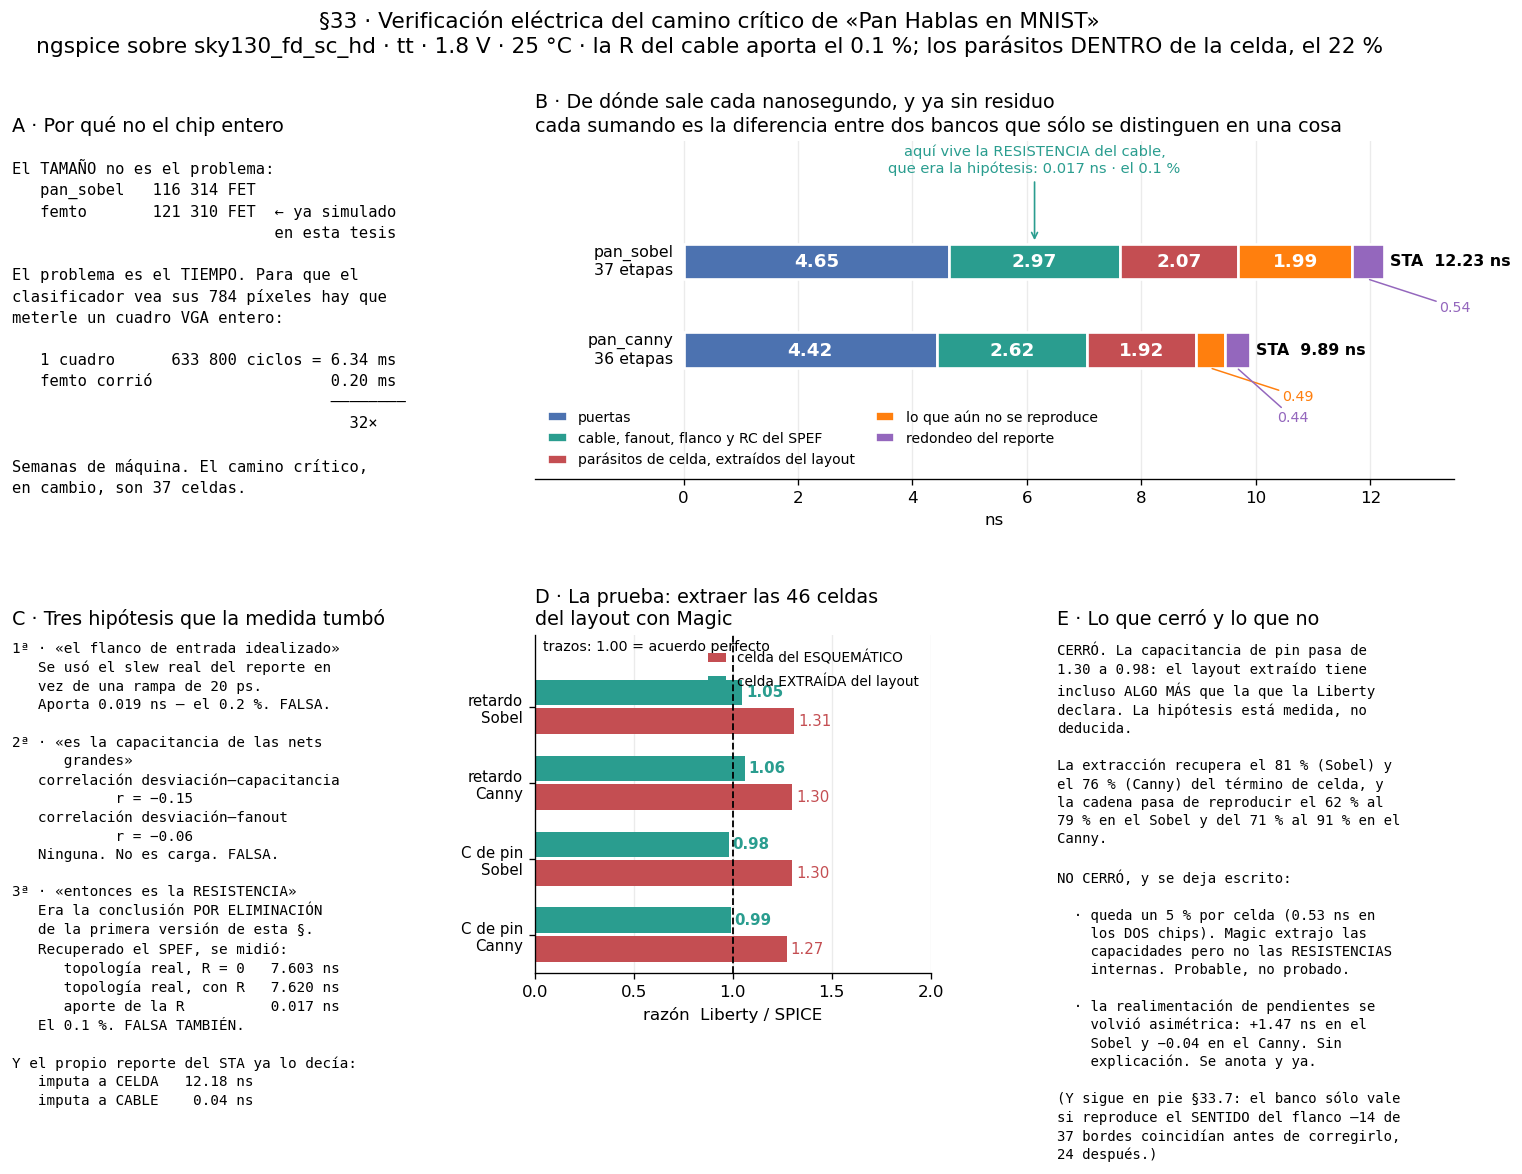
\includegraphics[keepaspectratio,alt={Figura 5.8. El desglose completo de la verificación. El panel A explica por qué se simula el camino y no el chip; el B reparte los 12,23 ns del pan\_sobel y los 9,89 del pan\_canny en sumandos que no dejan residuo; el C recoge las tres hipótesis que la medida desmintió; el D contrapone la celda del esquemático con la extraída del dibujo en los dos experimentos independientes; y el E separa lo que quedó cerrado de lo que se deja escrito como abierto.}]{figuras/fig_5_8_spice_desglose.png}}
\caption{\textbf{Figura 5.8.} El desglose completo de la verificación.
El panel A explica por qué se simula el camino y no el chip; el B
reparte los 12,23 ns del \texttt{pan\_sobel} y los 9,89 del
\texttt{pan\_canny} en sumandos que no dejan residuo; el C recoge las
tres hipótesis que la medida desmintió; el D contrapone la celda del
esquemático con la extraída del dibujo en los dos experimentos
independientes; y el E separa lo que quedó cerrado de lo que se deja
escrito como abierto.}
\end{figure}

\subsection{5.7.3 Tres explicaciones que la medida
desmintió}\label{tres-explicaciones-que-la-medida-desmintiuxf3}

Las tres parecían razonables, y conviene dejar constancia de las tres.

\textbf{El flanco de entrada idealizado.} El estímulo inicial era una
rampa de 20 ps, mucho más limpia que la transición que la primera etapa
recibe en el circuito; cabía esperar que un frente degradado se
propagase como retardo a lo largo de las treinta y siete etapas.
Sustituido por la pendiente real que el reporte declara, la contribución
resultó de \textbf{0,019 ns: el 0,2 \%}.

\textbf{La capacitancia de las redes grandes.} Las desviaciones mayores
se concentraban en puertas de muchas entradas, lo que sugería redes
largas y cargadas. Se midió la correlación entre la desviación de cada
etapa y su capacitancia: \textbf{r = −0,15}; y con el número de
destinos: \textbf{r = −0,06}. Ninguna de las dos sostiene la
explicación.

\textbf{La resistencia de la interconexión.} Descartadas las anteriores
quedaba ésta, y \textbf{así se dio por concluida la primera versión de
esta sección}: el analizador trabaja sobre el fichero de parásitos, que
informa resistencia y capacitancia de cada red, mientras que el reporte
de texto publica sólo la capacitancia, de modo que la simulación habría
recibido una descripción incompleta de los cables. La conjetura no pudo
comprobarse entonces porque ese fichero no se había conservado.

Recuperado, se midió. \textbf{La resistencia de la interconexión aporta
0,017 ns: el 0,1 \% del camino.} No los cuatro nanosegundos que había
que explicar.

\begin{quote}
\textbf{El propio reporte lo decía, y no se leyó.} El analizador imputa
cada retardo a un pin, y los de pin de salida son de celda mientras que
los de pin de entrada son de cable. Sumados por separado a lo largo del
camino: \textbf{12,18 ns imputados a celda y 0,04 ns a cable}. La
herramienta nunca atribuyó el tiempo a la interconexión. Bastaba con
sumar dos columnas.
\end{quote}

\subsection{5.7.4 La causa: la celda del esquemático no es la celda del
silicio}\label{la-causa-la-celda-del-esquemuxe1tico-no-es-la-celda-del-silicio}

Si la diferencia está dentro de las celdas, hay que preguntárselo a una
celda sola. El banco se redujo al mínimo ---una celda, el arco que el
camino recorre, la pendiente y la carga que el reporte declara--- y se
hizo la misma pregunta dos veces: a la tabla caracterizada, interpolando
como hace el analizador, y al simulador, resolviendo los transistores
que el kit de diseño distribuye.

La tabla reproduce al analizador casi exactamente, lo que confirma que
éste se limita a consultarla. La simulación, en cambio, queda
\textbf{sistemáticamente por debajo en treinta y cinco de las treinta y
siete etapas}, con una razón de \textbf{1,31} que no depende ni de la
carga ni de la pendiente. Esa independencia es la que descarta un
defecto del banco y señala a la celda misma.

La causa está en el fichero que se le entregó como modelo. El kit
distribuye el netlist \textbf{esquemático}: doce transistores y ni un
solo parásito. La biblioteca caracterizada, en cambio, se obtuvo sobre
la celda \textbf{dibujada}, con el metal, los contactos y la difusión
que el \emph{layout} añade. Al simulador se le describió la celda antes
de dibujarla.

Eso admite medición directa. Inyectando una rampa lenta en cada pin de
entrada e integrando la corriente ---capacitancia como carga dividida
por tensión, sin modelo ni supuesto--- la biblioteca atribuye a cada
pin, en promedio sobre los treinta y cinco del camino, \textbf{un 30 \%
más de capacitancia de la que el esquemático tiene}.

\begin{quote}
\textbf{Dos experimentos distintos, la misma cifra.} La razón entre el
retardo que la biblioteca declara y el que la simulación obtiene sobre
el esquemático es \textbf{1,31}. La razón entre la capacitancia que la
biblioteca declara y la que el esquemático tiene es \textbf{1,30}. Uno
mide tiempos y el otro mide carga, sobre las mismas treinta y siete
etapas.
\end{quote}

\textbf{La comprobación.} Lo anterior establece que al esquemático le
faltan parásitos, no que sean \emph{ésos} los que faltan. El kit no
distribuye el netlist de la celda dibujada, pero sí el dibujo: se
extrajeron con Magic las \textbf{cuarenta y seis celdas} que aparecen en
los dos caminos y se repitieron los dos experimentos sin cambiar nada
más.

\begin{longtable}[]{@{}
  >{\raggedright\arraybackslash}p{(\linewidth - 4\tabcolsep) * \real{0.2727}}
  >{\raggedleft\arraybackslash}p{(\linewidth - 4\tabcolsep) * \real{0.3636}}
  >{\raggedleft\arraybackslash}p{(\linewidth - 4\tabcolsep) * \real{0.3636}}@{}}
\toprule\noalign{}
\begin{minipage}[b]{\linewidth}\raggedright
razón biblioteca / simulación
\end{minipage} & \begin{minipage}[b]{\linewidth}\raggedleft
celda del \textbf{esquemático}
\end{minipage} & \begin{minipage}[b]{\linewidth}\raggedleft
celda \textbf{extraída}
\end{minipage} \\
\midrule\noalign{}
\endhead
\bottomrule\noalign{}
\endlastfoot
capacitancia de pin · \texttt{pan\_sobel} & 1,30 & \textbf{0,98} \\
capacitancia de pin · \texttt{pan\_canny} & 1,27 & \textbf{0,99} \\
retardo de celda aislada · \texttt{pan\_sobel} & 1,31 & \textbf{1,05} \\
retardo de celda aislada · \texttt{pan\_canny} & 1,30 & \textbf{1,06} \\
\end{longtable}

\textbf{La discrepancia de capacitancia desaparece.} La hipótesis queda
medida y no deducida, que era justamente lo que faltaba.

\subsection{5.7.5 La cuenta, y lo que queda
abierto}\label{la-cuenta-y-lo-que-queda-abierto}

Repartidos los 12,230 ns sin residuo, el término que importa sale igual
en los dos circuitos:

\begin{longtable}[]{@{}
  >{\raggedright\arraybackslash}p{(\linewidth - 4\tabcolsep) * \real{0.2727}}
  >{\raggedleft\arraybackslash}p{(\linewidth - 4\tabcolsep) * \real{0.3636}}
  >{\raggedleft\arraybackslash}p{(\linewidth - 4\tabcolsep) * \real{0.3636}}@{}}
\toprule\noalign{}
\begin{minipage}[b]{\linewidth}\raggedright
\end{minipage} & \begin{minipage}[b]{\linewidth}\raggedleft
\texttt{pan\_sobel}
\end{minipage} & \begin{minipage}[b]{\linewidth}\raggedleft
\texttt{pan\_canny}
\end{minipage} \\
\midrule\noalign{}
\endhead
\bottomrule\noalign{}
\endlastfoot
\textbf{el modelo de celda, como fracción del camino} & \textbf{22,6 \%}
& \textbf{22,1 \%} \\
resistencia de la interconexión & 0,1 \% & 0,2 \% \\
\end{longtable}

Dos circuitos distintos, dos caminos críticos que no comparten una sola
instancia, y la misma cifra a cuatro décimas de punto: \textbf{algo más
de la quinta parte del retardo de un camino crítico la ponen los
parásitos que el dibujo añade dentro de las celdas.}

\begin{figure}
\centering
\pandocbounded{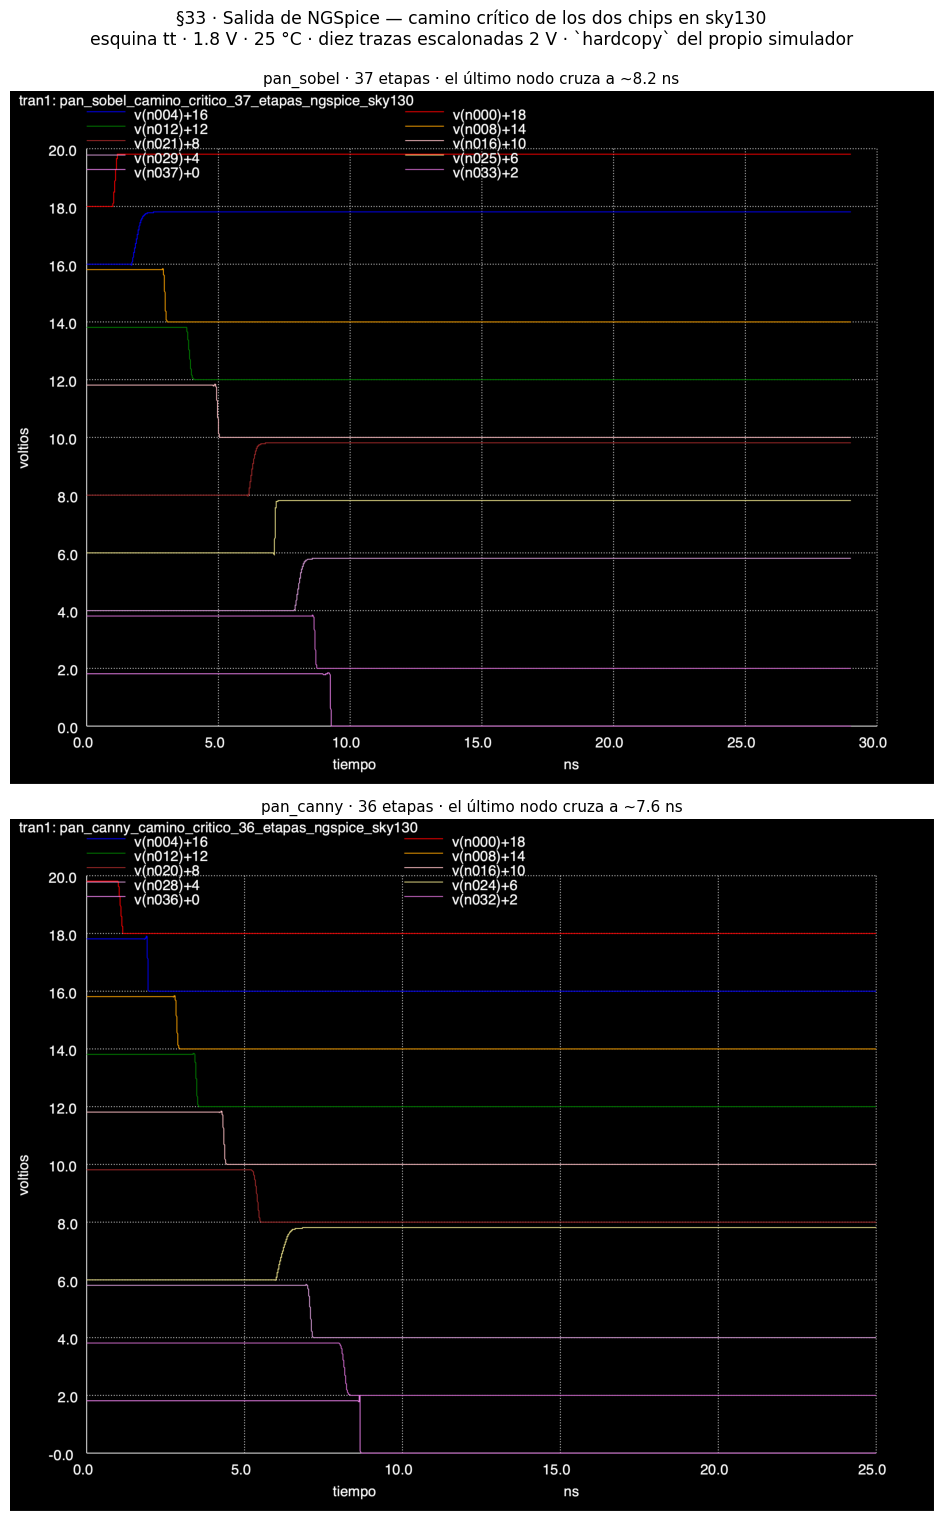
\includegraphics[keepaspectratio,alt={Figura 5.9. La salida del simulador, tal como éste la dibuja. Cada traza es un nodo del camino crítico, desplazada dos voltios respecto de la anterior para que las diez quepan en el mismo eje; la cascada de transiciones de arriba abajo es la señal propagándose etapa por etapa. El último nodo del pan\_sobel conmuta a unos 8,2 ns y el del pan\_canny a unos 7,6, que son las variantes D de la tabla anterior.}]{figuras/fig_5_9_spice_ondas.png}}
\caption{\textbf{Figura 5.9.} La salida del simulador, tal como éste la
dibuja. Cada traza es un nodo del camino crítico, desplazada dos voltios
respecto de la anterior para que las diez quepan en el mismo eje; la
cascada de transiciones de arriba abajo es la señal propagándose etapa
por etapa. El último nodo del \texttt{pan\_sobel} conmuta a unos 8,2 ns
y el del \texttt{pan\_canny} a unos 7,6, que son las variantes D de la
tabla anterior.}
\end{figure}

\textbf{Lo que no cerró, y se deja escrito.} Queda un 5 \% por celda
---0,528 ns en un chip y 0,530 en el otro, prácticamente el mismo valor
absoluto en dos caminos distintos--- que la extracción no recupera. La
explicación más probable es que el procedimiento empleado conserva las
\textbf{capacidades} internas de la celda pero no sus
\textbf{resistencias}, de modo que su metal interno sigue comportándose
como un cortocircuito ideal. Se anota como \textbf{probable y no
comprobada}. Y la realimentación de pendientes a lo largo de la cadena
resulta asimétrica entre los dos chips ---+1,47 ns en uno y −0,04 en el
otro--- sin explicación disponible.

\begin{quote}
\textbf{La conclusión.} El simulador y el analizador no discrepan sobre
la física: discrepan sobre el circuito. Al analizador se le describió la
celda tal como quedó en el \emph{layout}; al simulador, tal como estaba
en el esquema.

La verificación eléctrica no midió, por tanto, que el analizador se
equivocara. Midió \textbf{cuánto del retardo de un circuito integrado lo
pone el dibujo y no el esquema}: algo más de la quinta parte, y la misma
fracción en dos chips independientes. Es una cifra más útil que la que
se buscaba, y explica por qué ninguna implementación puede firmarse
sobre el esquemático.
\end{quote}

\chapter{6. Discusión}\label{discusiuxf3n}

\begin{quote}
\textbf{Estado:} borrador 1, escrito el 2026-09-21. Fuente: cuadernos 1
y 2, y el Capítulo 5. Formato Markdown para convertir con
\texttt{pandoc}.
\end{quote}

El capítulo anterior presentó mediciones. Éste sostiene afirmaciones. La
diferencia importa: una medición es un hecho que se comprueba repitiendo
el experimento, mientras que una afirmación es una lectura de varios
hechos y puede ser equivocada aunque todos ellos sean correctos. Este
trabajo tuvo que retractar dos afirmaciones de ese tipo durante su
desarrollo, y la experiencia dejó una disciplina que se aplica aquí:
\textbf{cada tesis de este capítulo señala qué medición la sostiene y
qué otra lectura descarta.}

\section{6.1 Lo que decide si un algoritmo cabe no es el
algoritmo}\label{lo-que-decide-si-un-algoritmo-cabe-no-es-el-algoritmo}

Ésta es la afirmación central del trabajo, y la más contraintuitiva para
quien llega desde el software.

Los tres filtros implementados ejecutan aritmética comparable. Ninguno
multiplica; los tres recorren la imagen aplicando una ventana de 3×3 y
comparando contra un umbral. Si el costo en silicio siguiera a la
complejidad aritmética, los tres deberían costar aproximadamente lo
mismo. La §5.4.3 midió lo contrario:

\begin{longtable}[]{@{}llr@{}}
\toprule\noalign{}
desde & hasta & cuesta \\
\midrule\noalign{}
\endhead
\bottomrule\noalign{}
\endlastfoot
Sobel & Canny de un salto & \textbf{+5 851 celdas} \\
Canny de un salto & Canny transitivo & \textbf{+94 511 celdas} \\
\end{longtable}

Ampliar el alcance de la ventana en un salto cuesta menos de seis mil
celdas. Ampliarlo al cuadro completo cuesta \textbf{noventa y cuatro mil
quinientas once}. Y la causa no está en las operaciones sino en
\textbf{cuánto estado hay que sostener a la vez}: los dos primeros
filtros procesan en flujo y retienen unas pocas líneas; el tercero
necesita el cuadro entero residente y accesible en orden arbitrario,
porque su punto fijo puede propagar una decisión desde cualquier píxel
hacia cualquier otro.

La comparación que resume el capítulo es ésta: \textbf{un procesador
RISC-V completo, con su memoria de programa y su periférico, cuesta
alrededor de nueve mil celdas} ---medido tres veces, sobre los tres
filtros, con una dispersión inferior al 5 \%--- \textbf{es decir,
aproximadamente la décima parte de lo que cuesta cambiar el alcance del
patrón de local a global.}

\begin{quote}
Dicho de otro modo: en el presupuesto de este chip, \textbf{meter un
procesador entero es una decisión menor comparada con decidir cuánta
imagen mira el filtro}. Es exactamente lo contrario de lo que sugiere la
intuición formada en software, donde el procesador es el recurso caro y
la memoria se pide al sistema operativo.
\end{quote}

\subsection{Las tres caras del mismo
precio}\label{las-tres-caras-del-mismo-precio}

El costo de la memoria no se cobra sólo en área. La §5.4.1 muestra que
\textbf{los dos circuitos transitivos son también los dos únicos que no
cierran temporizado}, con −19,35 ns y −18,23 ns de holgura una vez
extraídos los parásitos. El multiplexor que lee un framebuffer de miles
de entradas es un camino largo por construcción, y a partir de cierto
tamaño deja de ser caro para volverse inviable.

Y se cobra en manufacturabilidad. La §5.3 documenta que los diseños con
framebuffer grande acumulan un número de violaciones de antena muy
superior al resto, porque las redes de direccionamiento son largas y
ramificadas.

\textbf{Área, frecuencia y manufacturabilidad son tres manifestaciones
del mismo hecho}, y conviene presentarlas juntas: un diseñador que
optimice sólo el área concluirá que el framebuffer es aceptable, porque
sólo verá un tercio del problema.

\section{6.2 El costo se movió; no se
eliminó}\label{el-costo-se-moviuxf3-no-se-eliminuxf3}

Una lectura apresurada del clasificador de la §5.6 sugeriría que la
solución al problema anterior es sustituir memoria por lógica. El
trabajo permite matizar eso con números propios.

El clasificador de dígitos alcanza 91,04 \% sobre MNIST con \textbf{400
pesos de cuatro bits} ---doscientos bytes--- frente al 91,9 \% que
obtienen los 784 píxeles crudos con 7 840 pesos. La memoria se redujo en
un factor de veinte y la exactitud no se movió. Es un resultado fuerte,
y se enuncia así en la §5.6.

Pero el descriptor que hace posible esa reducción ---histograma de
orientaciones por zona, sobre bordes--- \textbf{no es gratuito}: hay que
calcularlo, y calcularlo es lógica. Las etapas cableadas que lo producen
cuestan decenas de miles de celdas.

\begin{quote}
La conclusión honesta no es «la codificación inteligente elimina el
costo» sino \textbf{«la codificación inteligente mueve el costo de
memoria a lógica»}, y eso es valioso únicamente porque en este sustrato
la memoria es el recurso caro. En una FPGA con bloques de memoria
disponibles, la misma decisión sería indiferente o incluso perjudicial.
\end{quote}

\section{6.3 Quién fija el reloj cambia con lo que se mete en el
chip}\label{quiuxe9n-fija-el-reloj-cambia-con-lo-que-se-mete-en-el-chip}

Los resultados del Capítulo 5 permiten seguir el camino crítico a lo
largo de una familia de diseños y observar que \textbf{el responsable
cambia tres veces}:

\begin{longtable}[]{@{}
  >{\raggedright\arraybackslash}p{(\linewidth - 2\tabcolsep) * \real{0.5000}}
  >{\raggedright\arraybackslash}p{(\linewidth - 2\tabcolsep) * \real{0.5000}}@{}}
\toprule\noalign{}
\begin{minipage}[b]{\linewidth}\raggedright
Diseño
\end{minipage} & \begin{minipage}[b]{\linewidth}\raggedright
Quién fija la frecuencia
\end{minipage} \\
\midrule\noalign{}
\endhead
\bottomrule\noalign{}
\endlastfoot
Filtros solos & el camino de datos del filtro \\
Con procesador & \textbf{el FemtoRV32} \\
Con framebuffer grande & \textbf{el multiplexor de lectura del
framebuffer} \\
\end{longtable}

Es un resultado útil para quien planifique un sistema parecido, porque
implica que \textbf{optimizar el bloque que fue crítico en el diseño
anterior puede no mejorar nada}. La pregunta «¿qué limita mi
frecuencia?» no tiene una respuesta estable: tiene una respuesta por
configuración.

\section{6.4 Integrar no es sumar, pero sólo cuando el temporizado
aprieta}\label{integrar-no-es-sumar-pero-suxf3lo-cuando-el-temporizado-aprieta}

Dos observaciones de este trabajo parecen contradecirse, y el matiz está
en la diferencia.

Al integrar el procesador con el filtro Canny en un die apretado, el
resultado superó la predicción ingenua ---la suma de las partes--- en
unas 6 500 celdas. En otro diseño de la misma familia, con die holgado y
reloj relajado, el resultado quedó un \textbf{1,6 \% por debajo} de esa
predicción.

Las dos medidas son correctas. Lo que las separa es \textbf{si el flujo
tuvo que trabajar para cerrar temporizado}: cuando lo tuvo, insertó
amortiguadores y redimensionó celdas, y ese trabajo se cobra en área;
cuando no, el optimizador pudo además compartir lógica entre bloques y
el total salió menor que la suma.

\begin{quote}
La regla que se deja escrita no es «integrar cuesta más» sino:
\textbf{la penalización de integración no es una propiedad del diseño
sino del margen con que se le pide cerrar.} Un mismo sistema puede
costar más o menos que sus partes según el reloj que se le exija.
\end{quote}

\section{6.5 La restricción mueve la frontera entre software y
hardware}\label{la-restricciuxf3n-mueve-la-frontera-entre-software-y-hardware}

El episodio de la §5.2.4 es el ejemplo más claro de co-diseño de este
trabajo, y conviene leerlo con cuidado porque su lección no es la
evidente.

La histéresis transitiva calculada por software funcionaba correctamente
en simulación. Al intentar sintetizar el conjunto sobre la iCE40UP5K la
ocupación llegó al \textbf{127 \%}. Trasladada a hardware como camino de
datos, la misma función ocupa el \textbf{33 \%}.

Lo interesante no es que el hardware sea más eficiente, que es
esperable. Es que \textbf{la frontera entre lo que ejecuta el procesador
y lo que ejecuta la lógica dedicada no la fijó una preferencia de diseño
sino una medición de recursos}. Y que esa frontera \textbf{se mueve con
el sustrato}: en el ASIC, donde el área no está acotada por un
dispositivo fijo, el procesador vuelve a ser viable junto al transitivo
y cuesta las mismas nueve mil celdas que junto a cualquier otro filtro.

La misma pregunta de diseño tiene respuestas opuestas en los dos
destinos, y ninguna de las dos es incorrecta.

\section{6.6 El front-end y el procesador son alternativas, no
complementos}\label{el-front-end-y-el-procesador-son-alternativas-no-complementos}

Éste es el aporte de ingeniería que el trabajo propone, y se apoya en
tres mediciones independientes.

\textbf{Primera.} Los dos filtros no se distinguen en exactitud de
clasificación: 0,38 pp entre ellos (§5.6). El Canny no reconoce mejor.

\textbf{Segunda.} Sí se distinguen en \textbf{sensibilidad al punto de
operación}. Mover el umbral cambia el resultado del Sobel en
\textbf{5,79 pp} y el del Canny en \textbf{0,90 pp}. El Sobel vive en un
pico angosto del espacio de parámetros; el Canny, en una meseta.

\textbf{Tercera.} Un Sobel sensible al umbral necesita que alguien se lo
ajuste en tiempo de ejecución, y para eso está el procesador con su
periférico. Un Canny insensible no lo necesita.

Poniendo precio a las dos soluciones sobre el mismo silicio:

\begin{longtable}[]{@{}
  >{\raggedright\arraybackslash}p{(\linewidth - 4\tabcolsep) * \real{0.3000}}
  >{\raggedright\arraybackslash}p{(\linewidth - 4\tabcolsep) * \real{0.3000}}
  >{\raggedleft\arraybackslash}p{(\linewidth - 4\tabcolsep) * \real{0.4000}}@{}}
\toprule\noalign{}
\begin{minipage}[b]{\linewidth}\raggedright
lo que se compra
\end{minipage} & \begin{minipage}[b]{\linewidth}\raggedright
dónde
\end{minipage} & \begin{minipage}[b]{\linewidth}\raggedleft
cuesta
\end{minipage} \\
\midrule\noalign{}
\endhead
\bottomrule\noalign{}
\endlastfoot
robustez al umbral \textbf{en el front-end} & el Canny, en el
reconocedor & \textbf{972 celdas} \\
robustez al umbral \textbf{por software} & el procesador y su periferia
& \textbf{6 220 celdas} \\
\end{longtable}

\begin{figure}
\centering
\pandocbounded{
\includegraphics[keepaspectratio,alt={Figura 6.1. El balance completo entre los dos filtros, sobre seis parejas de circuitos con plano firmado. El panel A los compara en celdas; el B muestra el sobrecoste del Canny cayendo del 123 \% al 3 \% conforme crece el sistema; el C corrige la lectura fácil ---el sobrecoste no es una cantidad fija, y lo que lo separa no es el tamaño del chip sino el de la imagen que el filtro recorre---; el D reúne las otras tres balanzas; y el E pone lado a lado las dos formas de comprar robustez al umbral.}]{figuras/fig_6_1_sobel_contra_canny.png}}
\caption{\textbf{Figura 6.1.} El balance completo entre los dos filtros,
sobre seis parejas de circuitos con plano firmado. El panel A los
compara en celdas; el B muestra el sobrecoste del Canny cayendo del 123
\% al 3 \% conforme crece el sistema; el C corrige la lectura fácil
---el sobrecoste \textbf{no} es una cantidad fija, y lo que lo separa no
es el tamaño del chip sino el de la imagen que el filtro recorre---; el
D reúne las otras tres balanzas; y el E pone lado a lado las dos formas
de comprar robustez al umbral.}
\end{figure}

\textbf{Comprar robustez en el front-end resulta unas seis veces más
barato que comprarla con un procesador.} Los dos caminos resuelven el
mismo problema ---que el punto de operación correcto depende de la
escena--- y la elección entre ellos es de arquitectura, no de algoritmo.

\begin{quote}
\textbf{Tres precisiones, porque la cifra se presta a mal uso.}

\emph{Primera: el factor depende de la escala de recuento, y por eso se
da redondeado.} Sobre celdas emplazadas la razón es \textbf{6,4}; sobre
celdas de síntesis, \textbf{8,0}. La diferencia no es un error de medida
sino un hecho: al emplazar, el sobrecoste del Canny crece un 48 \% y el
del procesador sólo un 18 \%, porque el primero es lógica en serie que
exige amortiguadores y el segundo es en buena parte memoria ya compacta.
\textbf{La conclusión cualitativa es robusta a la escala; el número
exacto no lo es}, y se enuncia como «unas seis veces» y no como «6,40».

\emph{Segunda: el numerador y el denominador no proceden del mismo
circuito.} El sobrecoste del Canny se mide sobre el par de
reconocedores, que recorren una ventana de 28×28; el del procesador,
sobre el par de filtros, que recorren la escena a 60×80. No existe un
reconocedor sin procesador en la misma tecnología con el que hacer la
resta directa, de modo que \textbf{la comparación es entre dos sistemas
emparentados y no entre dos versiones del mismo}. Se deja dicho porque
un lector podría suponer lo segundo.

\emph{Tercera: la resta de la derecha incluye} el FemtoRV32, su
controlador y su periférico, no sólo el núcleo: es lo que cuesta
\emph{poder escribir el umbral}, que es lo que se compara. Y la de la
izquierda es el sobrecoste del Canny \textbf{en ese sistema concreto};
la §5.4 muestra que en un circuito que procese la escena completa sería
mucho mayor. La afirmación vale para sistemas de reconocimiento sobre
ventana pequeña, no universalmente.
\end{quote}

\subsection{Sobre la trayectoria de este
argumento}\label{sobre-la-trayectoria-de-este-argumento}

Conviene dejar constancia de que \textbf{esta tesis sustituye a otra
anterior que resultó falsa}. Durante el desarrollo se sostuvo que el
Canny superaba al Sobel bajo condiciones de cámara degradadas. Al
revisarlo se comprobó que la comparación enfrentaba dos \emph{puntos de
operación} distintos y no dos filtros, y con el umbral efectivamente
implementado el resultado se invertía. Aquella justificación se
retractó.

El argumento que la reemplaza es más fuerte precisamente porque no
depende de una condición simulada sino de una \textbf{propiedad
estructural del algoritmo}: la histéresis es un mecanismo de
recuperación, y un mecanismo de recuperación es por definición menos
sensible a dónde se ponga el umbral.

\section{6.7 Mejor detección de bordes no implica mejor
reconocimiento}\label{mejor-detecciuxf3n-de-bordes-no-implica-mejor-reconocimiento}

El filtro transitivo produce los contornos visualmente más completos de
los tres: cierra siluetas, rellena trazos interrumpidos y elimina el
ruido aislado. Por cualquier criterio visual es el mejor detector de
bordes del trabajo.

Y \textbf{no es el mejor front-end para el clasificador}. Las métricas
de la §5.6 muestran que ordena bien las hipótesis pero calibra mal:
engordar los contornos aumenta el número de píxeles de borde, y como el
descriptor cuenta píxeles por zona, esa ganancia visual se traduce en
falsos positivos.

Hay además una razón arquitectónica, y es la más importante: \textbf{el
transitivo no puede operar en flujo}. Necesita el cuadro completo y un
número de barridos que depende de la imagen. No es un filtro más caro
que los otros dos ---\textbf{es otra clase de objeto computacional}, y
compararlo con ellos en área o en latencia oculta esa diferencia de
naturaleza.

\section{6.8 Una jerarquía construida, no
esperada}\label{una-jerarquuxeda-construida-no-esperada}

El clasificador implementa explícitamente la jerarquía \emph{bordes →
orientaciones → zonas → dígito}. Esa descomposición se propone
habitualmente como una \textbf{esperanza} sobre lo que aprenden las
capas ocultas de una red neuronal, y es sabido que rara vez ocurre así.

Aquí ocurre porque \textbf{está escrita}: cada etapa existe como
hardware identificable, sus salidas son inspeccionables y su
comportamiento es el que su nombre indica. El costo de esa transparencia
es que alguien tuvo que decidir la descomposición en lugar de
aprenderla.

\begin{quote}
Con la salvedad honesta de la §6.2: los 400 pesos de cuatro bits son
doscientos bytes frente a los decenas de kilobytes de una red
equivalente, pero \textbf{las etapas cableadas que producen el
descriptor cuestan decenas de miles de celdas}. La comparación de
memorias es correcta y la de sistemas completos sería otra.
\end{quote}

\section{6.9 Lo que el esquemático no
muestra}\label{lo-que-el-esquemuxe1tico-no-muestra}

Un resultado lateral, surgido al generar los esquemáticos RTL del
Capítulo 5, ilustra el problema central desde un ángulo inesperado.

En la vista RTL de cualquier herramienta, \textbf{un framebuffer es un
rectángulo} ---con una dirección de entrada y un dato de salida---
dibujado del mismo tamaño que un sumador. El esquemático no distingue
entre una memoria y una compuerta.

En silicio, ese mismo rectángulo son \textbf{6 400 biestables} que
ocupan un tercio del circuito, para almacenar 784 bytes.

\begin{quote}
\textbf{La abstracción que hace legible el diagrama es precisamente la
que oculta el costo dominante.} Un diseñador que razone sobre la vista
RTL llegará sistemáticamente a la conclusión equivocada sobre qué parte
de su circuito es cara, y no porque la herramienta mienta, sino porque
representa con la misma tinta cosas cuyo precio difiere en tres órdenes
de magnitud.
\end{quote}

\section{6.10 Posición frente a los trabajos
cercanos}\label{posiciuxf3n-frente-a-los-trabajos-cercanos}

Dos trabajos del mismo grupo sirven de referencia. El primero implementa
un Sobel en escala de grises sobre sky130 mediante Tiny Tapeout; el
segundo, un SoC basado en FemtoRV32 con memorias externas.

Con el primero, la expresión del gradiente es la misma,
\texttt{\textbar{}Gx\textbar{}+\textbar{}Gy\textbar{}}, de modo que en
Sobel puro ambas implementaciones son equivalentes. \textbf{La
diferencia es de alcance y no de calidad}: aquí hay procesador, tres
filtros seleccionables, cadena completa con cámara y pantalla, y un
clasificador. Conviene decirlo así explícitamente, porque presentar un
trabajo cercano como inferior cuando simplemente abordaba otra pregunta
es tanto una imprecisión como una descortesía.

Frente a la literatura de aceleradores de visión, la contribución de
este trabajo no es un detector mejor ---los algoritmos son de 1968, 1986
y 1993--- sino \textbf{una comparación sistemática de dos front-ends
sobre silicio firmado, a igualdad de todo lo demás, a lo largo de seis
sistemas de complejidad creciente}. Esa condición de igualdad es lo que
permite atribuir cada diferencia a una causa.

\section{6.11 Limitaciones}\label{limitaciones}

\begin{itemize}
\tightlist
\item
  \textbf{Ningún circuito ha sido fabricado.} Todas las afirmaciones
  sobre silicio se refieren a GDSII firmado con DRC, LVS y XOR en cero,
  no a medidas sobre un dado real.
\item
  \textbf{Las resoluciones son pequeñas}: 60×80 y 160×120 para el
  procesamiento, 28×28 para el reconocimiento. Son exactamente lo que la
  memoria disponible permite, y ese límite es el objeto de estudio, pero
  conviene no extrapolar los resultados a resoluciones mayores sin
  volver a medir.
\item
  \textbf{La magnitud del gradiente satura a ocho bits}, lo que en
  escenas de alto contraste recorta la información antes del umbral.
\item
  \textbf{Los recuentos de celdas no son homogéneos} entre todas las
  tablas del Capítulo 5, por las tres definiciones documentadas en la
  §5.3.3. Los cocientes dentro de cada pareja son válidos; las
  comparaciones absolutas entre tablas distintas, no.
\item
  \textbf{La verificación eléctrica de la §5.7 deja un residuo
  declarado}: la extracción del layout de las celdas recupera la mayor
  parte de la discrepancia entre SPICE y el analizador estático, pero no
  toda, y la parte restante se atribuye a la resistencia interna de la
  celda sin haberlo comprobado.
\end{itemize}

\chapter{7. Conclusiones y trabajo
futuro}\label{conclusiones-y-trabajo-futuro}

\begin{quote}
\textbf{Estado:} borrador 2, 2026-09-21. La §7.1 se leyó objetivo por
objetivo contra la §1.4 y responde a los cinco; el título está decidido.
\end{quote}

\section{7.1 Conclusiones por objetivo}\label{conclusiones-por-objetivo}

\textbf{Sobre el modelo de referencia.} Se construyó un modelo en Python
de los tres filtros y del clasificador, y se usó como verdad de
referencia en lugar de como ilustración. La decisión de escribirlo
\emph{antes} que el RTL permitió que la verificación fuera una
comparación numérica y no una inspección visual, lo que a su vez hizo
detectables errores ---un desplazamiento de fila, una saturación, un
signo invertido--- que producen salidas de aspecto correcto.

\textbf{Sobre la verificación.} Los tres núcleos de filtrado resultaron
\textbf{idénticos bit a bit} al modelo: cero píxeles de diferencia sobre
4 800, en las cinco imágenes de prueba. El clasificador se sometió a una
prueba más exigente ---las \textbf{diez mil} imágenes del conjunto de
evaluación de MNIST, comparadas una por una--- y el resultado fue el
mismo: \textbf{diez mil predicciones y diez mil veredictos de rechazo
idénticos}, con la matriz de confusión coincidiendo casilla por casilla.
Esa exactitud no es fortuita sino consecuencia de haber elegido una
aritmética que la admite ---enteros, pesos que son potencias de dos,
norma L1, umbral por comparación---, y constituye por tanto una
conclusión de diseño y no sólo de verificación.

\textbf{Sobre la integración en FPGA.} El sistema completo ---cámara,
tres filtros seleccionables, procesador RISC-V y pantalla--- funciona
\textbf{físicamente} sobre una iCE40UP5K. Enfrentado a dígitos
manuscritos sostenidos ante la cámara, el sistema con front-end Canny
\textbf{reconoció nueve de diez}, coincidiendo con lo que la simulación
predecía. Y en un segundo ensayo con diez dígitos grabados en el propio
\emph{bitstream}, el circuito reprodujo la simulación \textbf{incluidos
sus dos errores}: los mismos dos dígitos, con las mismas respuestas
equivocadas. Reproducir un acierto puede ser casualidad; reproducir un
error específico y repetido, no.

\textbf{Sobre el paso a silicio.} Se llevaron a GDSII \textbf{dieciséis
circuitos} en dos procesos ---sky130A con OpenLane e IHP SG13G2 con
LibreLane---, todos ellos con \textbf{DRC, LVS y XOR en cero}. La
verificación eléctrica se cerró por dos vías independientes: los
circuitos \textbf{cierran el temporizado con los parásitos del
interconexionado extraídos} ---holgura de 0,00 ns sobre el peor
camino---, y el camino crítico de \textbf{dos} de ellos se simuló además
en SPICE hasta repartir su retardo en sumandos sin residuo (§5.7).
Ninguno ha sido fabricado, y esa distinción se mantiene en todo el
documento: \textbf{silicio firmado no es silicio}.

\textbf{Sobre la medición de compromisos.} El objetivo que dio origen al
trabajo era medir qué cambia al cruzar de un sustrato al otro, en cuatro
dimensiones:

\begin{itemize}
\tightlist
\item
  \textbf{Área.} Es la dimensión que articula el Capítulo 6:
  \textbf{cambia el precio de la memoria, y ese precio decide qué
  algoritmo cabe.} Un procesador RISC-V completo cuesta alrededor de
  nueve mil celdas; ampliar el alcance del patrón de una ventana de 3×3
  al cuadro completo cuesta noventa y cuatro mil quinientas.
\item
  \textbf{Frecuencia.} En la FPGA el límite no lo pone la ocupación sino
  el procesador: las tres variantes que lo incorporan se agrupan en
  torno a los 9 MHz, con independencia de que ocupen el 91 \% o el 99 \%
  del dispositivo, mientras que la que prescinde de él alcanza 28,7 MHz.
  La causa está medida ---un camino de medio período que nace en el
  registro de instrucción--- y no se corrige emplazando mejor.
\item
  \textbf{Latencia.} Separa a las dos arquitecturas por \textbf{dos
  órdenes de magnitud} ---entre ochenta y trescientas veces:
  microsegundos el flujo, centenas de microsegundos por cuadro el
  transitivo---, y no por eficiencia de implementación sino porque una
  decide con información local y la otra necesita el cuadro entero. El
  procesador no la altera: contada en ciclos es la misma con él y sin
  él, porque escribe un registro de configuración y no participa del
  camino de datos de imagen.
\item
  \textbf{Manufacturabilidad.} Los diseños con memoria de cuadro grande
  acumulan violaciones de antena muy por encima del resto, porque sus
  redes de direccionamiento son largas y ramificadas.
\end{itemize}

\begin{quote}
Las tres primeras no son independientes: \textbf{área, frecuencia y
manufacturabilidad son tres manifestaciones del mismo hecho.} Quien
optimice sólo el área concluirá que la memoria de cuadro es aceptable,
porque habrá visto un tercio del problema.
\end{quote}

\section{7.2 Contribuciones}\label{contribuciones}

\begin{enumerate}
\def\labelenumi{\arabic{enumi}.}
\item
  \textbf{Un sistema de visión embebido completo y verificado}, con tres
  detectores de bordes seleccionables por software sobre video en vivo,
  funcionando físicamente en una FPGA de bolsillo y llevado a silicio
  firmado.
\item
  \textbf{Un motor de histéresis transitiva en hardware}, que resuelve
  la reconstrucción morfológica como punto fijo sin intervención del
  procesador, junto con el hallazgo de co-diseño que lo motivó: la misma
  función no cabía expresada como programa y ocupa un tercio del
  dispositivo expresada como circuito.
\item
  \textbf{Una comparación sistemática de dos front-ends sobre silicio
  firmado}, a igualdad de todo lo demás, a lo largo de seis sistemas de
  complejidad creciente. De ella se desprende el resultado de ingeniería
  que el trabajo propone: \textbf{el front-end y el procesador son
  alternativas para comprar robustez, no complementos}, y comprarla en
  el front-end resulta unas seis veces más barato.
\item
  \textbf{Un clasificador de patrones que cabe donde no cabe una red}:
  400 pesos de cuatro bits ---doscientos bytes--- alcanzan sobre MNIST
  la misma exactitud que los 784 píxeles crudos con la vigésima parte de
  la memoria, y el circuito reproduce ese resultado sin discrepancia.
\item
  \textbf{Dos cuadernos reproducibles} que contienen el código, los
  datos y las figuras de cada afirmación del documento, incluidas las
  que fueron corregidas.
\end{enumerate}

\section{7.3 Seis afirmaciones propias que este trabajo
corrigió}\label{seis-afirmaciones-propias-que-este-trabajo-corrigiuxf3}

Se listan porque forman parte del resultado. Un documento que enumera
sus propios errores con fecha y evidencia es más difícil de atacar que
uno que no enumera ninguno; y un jurado que encuentra un error por su
cuenta es mucho peor que uno que lo ve ya corregido.

\begin{longtable}[]{@{}
  >{\raggedright\arraybackslash}p{(\linewidth - 4\tabcolsep) * \real{0.3333}}
  >{\raggedright\arraybackslash}p{(\linewidth - 4\tabcolsep) * \real{0.3333}}
  >{\raggedright\arraybackslash}p{(\linewidth - 4\tabcolsep) * \real{0.3333}}@{}}
\toprule\noalign{}
\begin{minipage}[b]{\linewidth}\raggedright
\#
\end{minipage} & \begin{minipage}[b]{\linewidth}\raggedright
Lo que se afirmó
\end{minipage} & \begin{minipage}[b]{\linewidth}\raggedright
Lo que la medida mostró
\end{minipage} \\
\midrule\noalign{}
\endhead
\bottomrule\noalign{}
\endlastfoot
1 & Una señal de sincronismo ausente en el sensor & Era un
desplazamiento de uno en el conteo de línea \\
2 & Un umbral óptimo hallado sobre 20 000 imágenes & No se transfiere al
conjunto completo de 60 000 \\
3 & Una exactitud del \textbf{97,3 \%} & Provenía de un defecto del
banco de medida \\
4 & Una dispersión estimada con cinco semillas & \textbf{Subestimada en
un factor de 1,8} por solapamiento de las submuestras \\
5 & El Canny supera al Sobel bajo condiciones degradadas & Comparaba
\textbf{dos puntos de operación}, no dos filtros; con el umbral
implementado el resultado se invierte \\
6 & La discrepancia entre SPICE y el analizador estático es la
\textbf{resistencia} de la interconexión & La resistencia aporta
\textbf{0,017 ns}, el 0,1 \%. La causa son los parásitos internos de la
celda (§5.7.3) \\
\end{longtable}

Las seis comparten una forma, y conviene enunciarla porque es la lección
metodológica del trabajo: \textbf{ninguna procedía de una medición
equivocada.} Las mediciones eran correctas en todos los casos. Lo que
falló fue la lectura: comparar en puntos de operación distintos, estimar
la variabilidad con un procedimiento sesgado, confiar en un instrumento
sin verificarlo, y ---en la sexta--- \textbf{tomar por conclusión lo que
era una hipótesis obtenida por eliminación}.

\begin{quote}
Una deducción por eliminación vale lo que valga la lista de alternativas
consideradas. En el caso de la sexta, aquella lista no incluía «el
modelo de celda del PDK es esquemático y no de layout», que era la
respuesta. La regla que se deja escrita: \textbf{las deducciones se
escriben como hipótesis hasta que exista una medida que las sostenga.}
\end{quote}

\section{7.4 Trabajo futuro}\label{trabajo-futuro}

\textbf{Fabricar.} Los circuitos están firmados pero no existen. La vía
practicable es un servicio de oblea compartida como Tiny Tapeout, que
reparte el costo entre cientos de diseños pequeños a cambio de caber en
mosaicos de dimensiones fijas. Los proyectos necesarios están preparados
y han superado los chequeos de admisión; lo que falta es enviarlos a una
ventana de fabricación.

\textbf{Sustituir los framebuffers de biestables por un macro de SRAM.}
Es la respuesta directa al hallazgo central. Todo el precio documentado
en el Capítulo 6 ---área, frecuencia y manufacturabilidad--- procede de
implementar memoria con lógica porque el flujo empleado no ofrecía otra
cosa. Un generador de memoria cambiaría los tres a la vez, y permitiría
cuantificar cuánto de lo medido es propiedad del problema y cuánto del
sustrato.

\textbf{Subir de resolución.} Las resoluciones empleadas ---60×80 y
160×120 para procesar, 28×28 para reconocer--- son exactamente lo que la
memoria disponible permite. Con almacenamiento adecuado, la pregunta de
si las conclusiones escalan es empírica y está abierta.

\textbf{Completar la matriz de reconocedores.} Los circuitos que
reconocen cubren dos de los tres front-ends del trabajo. Falta el
transitivo, cuya incorporación exige un extractor de características
nuevo y un reentrenamiento de los pesos. Su ausencia es además coherente
con el argumento: el transitivo es precisamente el que no cabe.

\textbf{Cerrar la verificación eléctrica.} La extracción del layout de
las celdas estándar recupera la mayor parte de la discrepancia entre
SPICE y el analizador estático, pero no toda. La fracción restante se
atribuye a la resistencia interna de la celda sin haberlo comprobado, y
comprobarlo exige repetir la extracción con resistencias.

\newpage

\chapter{Anexos}\label{anexos}

\section{Anexo A. El entorno de trabajo: dos máquinas y una
frontera}\label{anexo-a.-el-entorno-de-trabajo-dos-muxe1quinas-y-una-frontera}

\begin{quote}
\textbf{Estado:} borrador 1, escrito el 2026-09-21. Este anexo documenta
la infraestructura sobre la que se produjo todo el trabajo. Se incluye
porque es \textbf{ingeniería real que el cuerpo del documento no
muestra}: la §3.7 la resume en un párrafo, y ese párrafo esconde tanto
el reparto de herramientas como una clase de error que costó horas.
\end{quote}

\subsection{A.1 Por qué dos
máquinas}\label{a.1-por-quuxe9-dos-muxe1quinas}

El flujo completo ---del modelo en Python al GDSII firmado--- no se
ejecuta en un solo sitio. La razón no es de conveniencia sino de
disponibilidad: \textbf{parte de las herramientas no existe compiladas
para la arquitectura del equipo principal}, y otra parte depende de un
contenedor que sólo corre sobre Linux.

El reparto resultante es el siguiente, y conviene tenerlo escrito porque
determina dónde se reproduce cada resultado de este documento:

\begin{longtable}[]{@{}
  >{\raggedright\arraybackslash}p{(\linewidth - 4\tabcolsep) * \real{0.3333}}
  >{\raggedright\arraybackslash}p{(\linewidth - 4\tabcolsep) * \real{0.3333}}
  >{\raggedright\arraybackslash}p{(\linewidth - 4\tabcolsep) * \real{0.3333}}@{}}
\toprule\noalign{}
\begin{minipage}[b]{\linewidth}\raggedright
Etapa
\end{minipage} & \begin{minipage}[b]{\linewidth}\raggedright
Herramienta
\end{minipage} & \begin{minipage}[b]{\linewidth}\raggedright
Dónde corre
\end{minipage} \\
\midrule\noalign{}
\endhead
\bottomrule\noalign{}
\endlastfoot
Modelo de referencia & Python, NumPy & equipo principal \\
Simulación RTL y verificación & Icarus Verilog, cocotb & equipo
principal \\
Síntesis lógica & yosys & equipo principal \\
Simulación eléctrica & NGSpice & equipo principal \\
Esquemáticos RTL & yosys + netlistsvg & equipo principal \\
\textbf{Emplazamiento y ruteo en FPGA} & nextpnr-ice40, icepack &
\textbf{máquina virtual} \\
\textbf{Flujo completo a ASIC} & OpenLane sobre Docker & \textbf{máquina
virtual} \\
\textbf{Extracción de celdas, DRC, LVS} & Magic, Netgen &
\textbf{máquina virtual} \\
\textbf{Análisis estático de tiempos} & OpenSTA & \textbf{máquina
virtual} \\
\textbf{Visualización de layout} & KLayout con interfaz gráfica &
\textbf{máquina virtual} \\
Grabación del \emph{bitstream} & copia al volumen de la tarjeta & equipo
principal \\
\end{longtable}

La consecuencia práctica es que \textbf{un resultado de silicio no se
puede reproducir sin la máquina virtual}, mientras que toda la
verificación funcional y eléctrica sí se reproduce en el equipo
principal. Esa asimetría condiciona qué partes de este trabajo son
fácilmente auditables por un tercero.

\subsection{A.2 La frontera, y cómo se
cruza}\label{a.2-la-frontera-y-cuxf3mo-se-cruza}

Las dos máquinas comparten un directorio mediante \textbf{virtiofs},
montado en rutas distintas a cada lado:

\begin{verbatim}
equipo principal :  ~/utm-share
máquina virtual  :  /mnt/share/utm-share
\end{verbatim}

Sobre esa frontera cruzan tres clases de objeto, en direcciones
distintas:

\begin{itemize}
\tightlist
\item
  \textbf{Hacia la máquina virtual:} fuentes RTL, ficheros de
  configuración del flujo y guiones de ejecución.
\item
  \textbf{Hacia el equipo principal:} reportes de firma, ficheros de
  métricas, extracciones de parásitos y planos comprimidos.
\item
  \textbf{En ninguna dirección:} los directorios de ejecución completos,
  que ocupan cientos de megabytes por diseño y se archivan localmente en
  cada máquina.
\end{itemize}

\subsection{A.3 Una clase de error que conviene
documentar}\label{a.3-una-clase-de-error-que-conviene-documentar}

La frontera no es transparente, y su opacidad produce un error con una
firma característica: \textbf{la herramienta lee una versión del fichero
distinta de la que se escribió}.

Durante el desarrollo se corrigió un defecto en un fuente Verilog, se
verificó la corrección en el equipo principal ---contenido y suma de
comprobación--- y se copió al directorio compartido. La máquina virtual,
sin embargo, siguió sirviendo el contenido anterior. El flujo falló
\textbf{dos veces seguidas con el mismo error ya corregido} antes de que
se comprobara el fichero en su destino final.

La causa es la caché de lectura del sistema de ficheros compartido. El
procedimiento que la evita es elemental y se adoptó como regla:

\begin{enumerate}
\def\labelenumi{\arabic{enumi}.}
\tightlist
\item
  Copiar a una \textbf{ruta nueva} en lugar de sobrescribir la
  existente: un camino distinto no tiene caché previa.
\item
  Comprobar el fichero \textbf{desde la máquina que lo va a leer}, no
  desde la que lo escribió.
\item
  Comprobarlo \textbf{en su destino final}, no en el directorio
  compartido --- es decir, ya dentro del árbol de trabajo de la
  herramienta.
\end{enumerate}

\begin{quote}
Formulada como principio: \textbf{verificar el fichero donde la
herramienta va a leerlo, no donde uno lo escribió.} Es el mismo
razonamiento de la §3.6 aplicado a la infraestructura: el instrumento
---aquí, el canal entre las dos máquinas--- también puede mentir, y
también hay que verificarlo antes de confiar en lo que entrega.
\end{quote}

\subsection{A.4 Otras asimetrías
anotadas}\label{a.4-otras-asimetruxedas-anotadas}

Se listan porque cada una costó tiempo al descubrirse:

\begin{itemize}
\tightlist
\item
  \textbf{La ruta de instalación no es la que se supone.} El flujo a
  ASIC no reside en el directorio de inicio sino varios niveles más
  abajo, y el kit de diseño tampoco está donde su documentación sugiere.
  Un guion que asuma las rutas canónicas falla sin explicar por qué.
\item
  \textbf{Las capturas de layout requieren interfaz gráfica.} En modo
  desatendido, y sin encontrar el fichero de propiedades de capas, el
  visor produce una imagen uniforme e inservible. La limitación es del
  modo de invocación, no de la herramienta, y las figuras de este
  documento se obtuvieron con la interfaz.
\item
  \textbf{El contenedor del flujo a ASIC reescribe el directorio de
  inicio}, de modo que las operaciones que dependen de rutas absolutas
  del anfitrión ---fotografías, visualización--- deben ejecutarse fuera
  de él.
\item
  \textbf{El simulador de FPGA no dispone de visor de formas de onda
  funcional en el equipo principal}, por lo que la inspección de ondas
  se realiza en la máquina virtual sobre los ficheros generados en el
  principal.
\end{itemize}

\subsection{A.5 Reproducibilidad}\label{a.5-reproducibilidad}

Todo lo necesario para reproducir los resultados de este documento está
versionado, con dos excepciones declaradas:

\begin{itemize}
\tightlist
\item
  \textbf{Los planos completos} ---GDSII, DEF, vistas de Magic y
  extracciones de parásitos--- ocupan varios cientos de megabytes por
  circuito y viven fuera del repositorio, en un archivo local descrito
  por su propio índice. En el repositorio quedan las fuentes, los
  abstractos de celda, los reportes de firma y los ficheros de métricas.
\item
  \textbf{Los conjuntos de datos de entrenamiento y prueba} se descargan
  con un guion incluido, en lugar de versionarse.
\end{itemize}

Los guiones de cada figura y de cada tabla están en el repositorio junto
al capítulo que los usa, de modo que cualquier cifra de este documento
puede rastrearse hasta el comando que la produjo.

\section{Anexo B. Mapa de registros y
firmware}\label{anexo-b.-mapa-de-registros-y-firmware}

\begin{quote}
Fuente: \texttt{asic/soc\_sobel\_top/src/peripheral\_filter.v}.
\end{quote}

\subsection{B.1 El periférico de
control}\label{b.1-el-perifuxe9rico-de-control}

El procesador se comunica con el camino de imagen a través de un único
periférico mapeado en memoria en la base \textbf{\texttt{0x0045\_0000}}.
Su diseño obedece a la decisión de arquitectura de la §4.1: \textbf{los
píxeles no pasan por el bus}. El periférico expone tres registros y nada
más.

\begin{longtable}[]{@{}
  >{\raggedright\arraybackslash}p{(\linewidth - 6\tabcolsep) * \real{0.2500}}
  >{\raggedright\arraybackslash}p{(\linewidth - 6\tabcolsep) * \real{0.2500}}
  >{\raggedright\arraybackslash}p{(\linewidth - 6\tabcolsep) * \real{0.2500}}
  >{\raggedright\arraybackslash}p{(\linewidth - 6\tabcolsep) * \real{0.2500}}@{}}
\toprule\noalign{}
\begin{minipage}[b]{\linewidth}\raggedright
Desplazamiento
\end{minipage} & \begin{minipage}[b]{\linewidth}\raggedright
Nombre
\end{minipage} & \begin{minipage}[b]{\linewidth}\raggedright
Acceso
\end{minipage} & \begin{minipage}[b]{\linewidth}\raggedright
Campos
\end{minipage} \\
\midrule\noalign{}
\endhead
\bottomrule\noalign{}
\endlastfoot
\texttt{0x00} & \texttt{CTRL} & escritura & \texttt{{[}1:0{]}} modo ·
\texttt{{[}4{]}} habilitación · \texttt{{[}5{]}} reinicio del motor \\
\texttt{0x04} & \texttt{THR} & escritura & \texttt{{[}7:0{]}} umbral
bajo · \texttt{{[}15:8{]}} umbral alto \\
\texttt{0x08} & \texttt{STAT} & lectura & \texttt{{[}0{]}} configuración
terminada · \texttt{{[}1{]}} motor ocupado · \texttt{{[}2{]}}
sincronismo vivo · \texttt{{[}23:8{]}} cuenta de cuadros \\
\end{longtable}

El campo de modo selecciona cuál de los tres filtros procesa la imagen:

\begin{longtable}[]{@{}ll@{}}
\toprule\noalign{}
Valor & Filtro \\
\midrule\noalign{}
\endhead
\bottomrule\noalign{}
\endlastfoot
\texttt{0} & Sobel \\
\texttt{1} & Canny de un salto \\
\texttt{2} & Canny transitivo \\
\end{longtable}

\subsubsection{Dos decisiones de diseño visibles en la
tabla}\label{dos-decisiones-de-diseuxf1o-visibles-en-la-tabla}

\textbf{Los dos umbrales caben en una sola escritura.} El registro
\texttt{THR} empaqueta el umbral alto y el bajo en una palabra de 32
bits. No es una optimización de espacio sino de \textbf{atomicidad}:
escribir los dos umbrales del Canny en dos accesos separados deja al
filtro operando durante un intervalo con una pareja inconsistente ---un
umbral nuevo y otro viejo--- que puede producir un cuadro espurio. Una
sola escritura elimina ese estado transitorio.

\textbf{El estado incluye un indicador de vida.} El bit
\texttt{vsync\_alive} y la cuenta de cuadros permiten al programa
distinguir \emph{«el filtro no encuentra bordes»} de \emph{«la cámara
dejó de entregar imagen»}, que desde el punto de vista del procesador
producen la misma salida: un mapa vacío. Es un mecanismo de diagnóstico,
y su existencia procede directamente de los episodios documentados en la
§3.6.

\subsection{B.2 El firmware}\label{b.2-el-firmware}

El programa que ejecuta el procesador consta de \textbf{siete
instrucciones}. Su estructura es:

\begin{enumerate}
\def\labelenumi{\arabic{enumi}.}
\tightlist
\item
  Inicializar el puntero de pila.
\item
  Cargar la dirección base del periférico.
\item
  Escribir el modo y la habilitación en \texttt{CTRL}.
\item
  Escribir la pareja de umbrales en \texttt{THR}.
\item
  Entrar en un lazo de espera.
\end{enumerate}

No se trata de un programa reducido por limitación de memoria sino
\textbf{por diseño}: el procesador existe para poder cambiar un
parámetro en tiempo de ejecución, no para procesar imagen. Su presencia
se justifica por lo que habilita ---recalibrar el sistema sin volver a
sintetizar--- y no por el trabajo que realiza.

\begin{quote}
Ese es el punto que la §6.6 desarrolla: recalibrar un sistema con
procesador cuesta recompilar siete instrucciones; recalibrar uno sin
procesador cuesta un ciclo completo de síntesis, emplazamiento y ruteo.
La comparación entre ambas opciones es la que produce la razón 8:1.
\end{quote}

\subsection{B.3 La ROM en dos
sustratos}\label{b.3-la-rom-en-dos-sustratos}

El mismo programa se almacena de forma distinta según el destino, y ésta
es una de las cuatro diferencias obligatorias de la §4.8:

\begin{longtable}[]{@{}ll@{}}
\toprule\noalign{}
Destino & Implementación \\
\midrule\noalign{}
\endhead
\bottomrule\noalign{}
\endlastfoot
FPGA & arreglo inicializado desde el \emph{bitstream} \\
ASIC & \textbf{tabla de constantes sintetizada como lógica
combinacional} \\
\end{longtable}

En silicio no existe nada que cargue el contenido inicial de una
memoria. El código Verilog que funciona en ambos casos \textbf{simula
idénticamente} y produce circuitos distintos, de los cuales uno no
arranca. Es el ejemplo más claro de por qué la simulación RTL no basta
para validar un diseño destinado a fabricación.

\section{Anexo C. Asignación de
pines}\label{anexo-c.-asignaciuxf3n-de-pines}

\begin{quote}
Fuente: \texttt{clasificador\_mnist/fpga/mnist\_cam.pcf} --- el fichero
\textbf{efectivamente grabado y verificado sobre la tarjeta}, no una
transcripción.
\end{quote}

\subsection{C.1 La tarjeta}\label{c.1-la-tarjeta}

Las implementaciones físicas se realizaron sobre una \textbf{iCESugar
v1.5} con FPGA \textbf{iCE40UP5K}, una cámara \textbf{OV7670} y una
pantalla \textbf{TFT ILI9341} por SPI.

\subsection{C.2 Asignación}\label{c.2-asignaciuxf3n}

\begin{longtable}[]{@{}lrl@{}}
\toprule\noalign{}
Señal & Pin & Grupo \\
\midrule\noalign{}
\endhead
\bottomrule\noalign{}
\endlastfoot
\texttt{clk} & 35 & reloj de sistema \\
\texttt{cam\_xclk} & 2 & cámara --- reloj que se le entrega \\
\texttt{cam\_scl} & 27 & cámara --- reloj de configuración \\
\texttt{cam\_sda} & 26 & cámara --- dato de configuración \\
\texttt{cam\_pclk} & 28 & cámara --- reloj de píxel \\
\texttt{cam\_href} & 32 & cámara --- referencia de línea \\
\texttt{cam\_d{[}0{]}} & 48 & cámara --- bus de datos \\
\texttt{cam\_d{[}1{]}} & 46 & \\
\texttt{cam\_d{[}2{]}} & 44 & \\
\texttt{cam\_d{[}3{]}} & 43 & \\
\texttt{cam\_d{[}4{]}} & 38 & \\
\texttt{cam\_d{[}5{]}} & 34 & \\
\texttt{cam\_d{[}6{]}} & 31 & \\
\texttt{cam\_d{[}7{]}} & 42 & \\
\texttt{tft\_sck} & 37 & pantalla --- reloj SPI \\
\texttt{tft\_mosi} & 36 & pantalla --- dato \\
\texttt{tft\_cs} & 25 & pantalla --- selección \\
\texttt{tft\_dc} & 23 & pantalla --- dato/comando \\
\texttt{led\_r} & 39 & estado \\
\texttt{led\_g} & 40 & \\
\texttt{led\_b} & 41 & \\
\end{longtable}

\subsection{C.3 Una advertencia que costó media
hora}\label{c.3-una-advertencia-que-costuxf3-media-hora}

\textbf{Varios comentarios de cabecera de los fuentes de este trabajo
contienen la asignación equivocada} ---concretamente, \texttt{cam\_scl}
y \texttt{cam\_sda} aparecen intercambiados respecto de la tabla
anterior--- mientras que el fichero de restricciones tiene la correcta.

El origen es trivial: el comentario se escribió de memoria y el fichero
se ajustó por prueba. Pero la consecuencia no lo es, porque al preparar
un diseño nuevo la tentación es \textbf{transcribir} la asignación desde
el comentario en vez de \textbf{copiar} el fichero que ya funcionó.
Hacerlo produjo, en una ocasión, dos señales de estado cruzadas y media
hora de diagnóstico de un circuito que estaba bien.

\begin{quote}
La regla adoptada: \textbf{el fichero de restricciones probado manda
sobre cualquier comentario.} Al armar un diseño nuevo se copia, no se
transcribe.
\end{quote}

\subsection{C.4 El orden del bus de
datos}\label{c.4-el-orden-del-bus-de-datos}

Obsérvese que los ocho bits de la cámara \textbf{no ocupan pines
consecutivos ni ordenados}: el bit 7 está en el pin 42, entre el bit 3
(pin 43) y el bit 4 (pin 38). La asignación responde a la disposición
física del conector y no a ninguna lógica del diseño.

Esa irregularidad la hace especialmente propensa a errores de
transcripción, y fue el objeto de uno de los experimentos de diagnóstico
del desarrollo: un diseño que hacía que la propia tarjeta informara por
el puerto serie qué bits del bus estaban permanentemente a un valor
fijo, en lugar de inferirlo observando la imagen.

\section{Anexo D. Recetas del flujo a
silicio}\label{anexo-d.-recetas-del-flujo-a-silicio}

\begin{quote}
Fuente: los ficheros \texttt{config.json} de los veinte directorios de
diseño en sky130A. Esta tabla se generó leyéndolos, no
transcribiéndolos.
\end{quote}

\subsection{D.1 Qué se configura, y qué
no}\label{d.1-quuxe9-se-configura-y-quuxe9-no}

De los varios centenares de parámetros que admite el flujo, \textbf{sólo
cinco se tocaron} en todo el trabajo. El resto conserva su valor por
omisión, y esa contención es deliberada: cada parámetro modificado es
una variable más que explicar si un resultado sale distinto del
esperado.

\begin{longtable}[]{@{}
  >{\raggedright\arraybackslash}p{(\linewidth - 2\tabcolsep) * \real{0.5000}}
  >{\raggedright\arraybackslash}p{(\linewidth - 2\tabcolsep) * \real{0.5000}}@{}}
\toprule\noalign{}
\begin{minipage}[b]{\linewidth}\raggedright
Parámetro
\end{minipage} & \begin{minipage}[b]{\linewidth}\raggedright
Qué controla
\end{minipage} \\
\midrule\noalign{}
\endhead
\bottomrule\noalign{}
\endlastfoot
\texttt{CLOCK\_PERIOD} & el periodo objetivo, en nanosegundos \\
\texttt{FP\_CORE\_UTIL} & la fracción del núcleo que se pretende llenar
de celdas \\
\texttt{PL\_TARGET\_DENSITY} & la densidad objetivo del emplazador \\
\texttt{GRT\_ALLOW\_CONGESTION} & si se tolera congestión en el ruteo
global \\
\texttt{FP\_ASPECT\_RATIO} & la proporción del dado \\
\end{longtable}

\subsection{D.2 Las recetas empleadas}\label{d.2-las-recetas-empleadas}

\begin{longtable}[]{@{}lrrrc@{}}
\toprule\noalign{}
Diseño & Periodo & Utilización & Densidad & Congestión \\
\midrule\noalign{}
\endhead
\bottomrule\noalign{}
\endlastfoot
\texttt{cam\_frontend\_top} & 20 ns & 40 \% & 0,55 & --- \\
\texttt{lcd\_ili9341\_top} & 20 ns & 40 \% & 0,55 & --- \\
\texttt{sobel\_top} & 20 ns & 35 \% & --- & --- \\
\texttt{canny1\_top} & 20 ns & 35 \% & 0,45 & --- \\
\texttt{trans\_engine\_top} & 20 ns & 35 \% & 0,45 & --- \\
\texttt{soc\_sobel\_top} & 20 ns & 30 \% & 0,40 & --- \\
\texttt{soc\_canny1\_top} & 20 ns & 30 \% & 0,40 & --- \\
\texttt{soc\_trans\_top} & 20 ns & 18 \% & 0,25 & sí \\
\texttt{vision\_top} & 20 ns & 18 \% & 0,25 & sí \\
\texttt{vision\_canny\_top} & 20 ns & 18 \% & 0,25 & sí \\
\texttt{vision\_sobel\_mnist} & 20 ns & 18 \% & 0,25 & sí \\
\texttt{vision\_canny\_mnist} & 20 ns & 18 \% & 0,25 & sí \\
\texttt{pan\_sobel} & \textbf{30 ns} & 22 \% & 0,32 & sí \\
\texttt{pan\_canny} & \textbf{30 ns} & 22 \% & 0,32 & sí \\
\texttt{sobel\_completo} & 20 ns & 15 \% & 0,30 & sí \\
\texttt{canny1\_completo} & 20 ns & 15 \% & 0,20 & sí \\
\texttt{trans\_completo} & 20 ns & 15 \% & 0,20 & sí \\
\texttt{soc\_sobel\_completo} & \textbf{32 ns} & 15 \% & 0,20 & sí \\
\texttt{soc\_canny1\_completo} & \textbf{36 ns} & 15 \% & 0,20 & sí \\
\texttt{soc\_trans\_completo} & \textbf{36 ns} & 15 \% & 0,20 & sí \\
\end{longtable}

\begin{quote}
\textbf{Veinte recetas, dieciséis circuitos.} La tabla tiene más filas
que circuitos declara el Capítulo 7, y la diferencia merece explicarse.
Los seis diseños terminados en \texttt{\_completo} son una
\textbf{segunda vía} hacia el mismo sistema: mientras los
\texttt{vision\_*} se obtuvieron \textbf{portando el diseño físicamente
verificado en la FPGA}, los \texttt{\_completo} se \textbf{ensamblaron a
partir de los bloques reutilizables ya comprobados por separado}
---front-end de cámara, filtro, controlador de pantalla--- con un solo
dominio de reloj en lugar de dos. Ambas vías se ejecutaron; sólo la
primera se archivó con el expediente completo.

De los seis, tres ---\texttt{trans\_completo},
\texttt{soc\_canny1\_completo} y \texttt{soc\_trans\_completo}---
superaron las tres verificaciones de firma con cero observaciones, y
otros dos conservan el GDSII, pero \textbf{ninguno reúne a la vez el
GDSII y los tres informes} en el archivo curado. Por eso no se cuentan
entre los dieciséis: el criterio para contar un circuito en este trabajo
no es haberlo ejecutado, sino \textbf{poder mostrar el plano y las tres
firmas juntos}. Se dejan en esta tabla porque sus recetas son parte de
la evidencia del patrón que sigue, y porque omitirlos falsearía el
recuento de intentos.
\end{quote}

\subsection{D.3 El patrón que la tabla
revela}\label{d.3-el-patruxf3n-que-la-tabla-revela}

Leída de arriba abajo, la tabla cuenta la historia del proyecto, y
conviene señalarlo porque \textbf{ese patrón es un resultado y no una
casualidad}:

\textbf{La utilización desciende monótonamente con la complejidad del
diseño}, del 40 \% en los bloques de interfaz al 15 \% en los sistemas
completos. No es una preferencia estética: es que un diseño con mucha
memoria en biestables y muchos cruces de dominio \textbf{no rutea} a
densidad alta. La utilización que cada diseño admite es, en sí misma,
una medida indirecta de cuánta interconexión necesita.

\textbf{La tolerancia a congestión aparece exactamente donde aparece el
framebuffer.} Todos los diseños que la activan son los que almacenan un
cuadro; ninguno de los que procesan en flujo la necesita. Es la misma
frontera que separa las dos familias en la §5.5 ---por latencia--- y en
la §6.1 ---por área---, manifestada esta vez en el ruteo.

\textbf{El periodo sólo se relaja en los tres últimos.} Los tres llevan
procesador \emph{y} cadena completa, y son los únicos a los que no se
les pudo exigir 50 MHz. La §6.3 explica qué fija el reloj en cada caso.

\begin{quote}
Dicho de otro modo: \textbf{el mismo flujo, con el mismo kit y las
mismas celdas, exige recetas cada vez más conservadoras a medida que el
diseño almacena más estado.} El precio de la memoria no se manifiesta
sólo en el resultado, sino también en el esfuerzo que cuesta obtenerlo.
\end{quote}

\subsection{D.4 Sobre la elección de
utilización}\label{d.4-sobre-la-elecciuxf3n-de-utilizaciuxf3n}

La utilización no es una restricción física sino un objetivo que el
flujo intenta cumplir. Fijarla baja produce un dado más grande con ruteo
holgado; fijarla alta, uno más pequeño que puede no cerrar.

Durante el desarrollo se comprobó la relación de forma directa: un
diseño cerrado al 18 \% ocupa un dado de 2,03 mm², mientras que el mismo
diseño con una utilización del 35 \% debería aproximarse a 1,20 mm².
\textbf{La segunda cifra no está verificada}: el experimento quedó
preparado y no llegó a ejecutarse, y se anota aquí como tal para que no
se lea como medida.

\begin{quote}
La regla operativa que se siguió: \textbf{no se borra un resultado que
cerró para intentar mejorarlo.} Un experimento de ajuste se lanza
siempre con una etiqueta nueva, de modo que si el diseño apretado no
cierra, el firmado anterior permanece intacto. Un circuito que cierra
vale más que uno pequeño que no.
\end{quote}

\chapter{Bibliografía}\label{bibliografuxeda}

\begin{quote}
\textbf{Cómo se construyó esta lista.} Reúne las \textbf{36 referencias}
recopiladas a lo largo del cuaderno de laboratorio y las \textbf{17
verificadas contra la fuente} el 21 de septiembre de 2026 al redactar el
Capítulo 2. Ocho obras aparecían en ambas listas y se han fundido en una
sola entrada, conservando siempre los datos verificados; nueve son
aportación de la verificación, y una ---el libro de texto del que
procede la arquitectura de bus--- se añadió al documentar el linaje del
SoC en la §4.5. El total son \textbf{46 entradas sin duplicados}.

Las marcadas con \textbf{✓} tienen volumen, número, páginas y año
comprobados contra la fuente. Las demás son programas, kits de diseño,
hojas de datos o repositorios, que se citan por su identificador público
y no admiten esa comprobación.

Las notas introducidas por \textbf{▸} no señalan trabajo pendiente: son
\textbf{advertencias sobre la fuente misma} ---una obra que nunca se
publicó formalmente, otra que circula con dos numeraciones de volumen,
un título que cambió entre ediciones--- que un lector necesita para no
tomar por descuido lo que es una decisión. Deben permanecer en la
versión final.
\end{quote}

\section{Núcleo RISC-V y
arquitectura}\label{nuxfacleo-risc-v-y-arquitectura}

\begin{enumerate}
\def\labelenumi{\arabic{enumi}.}
\tightlist
\item
  B. Levy, \emph{FemtoRV32 / learn-fpga} --- núcleos RISC-V mínimos
  (Quark, RV32I). https://github.com/BrunoLevy/learn-fpga
\item
  B. Levy, \emph{FemtoRV32 DESIGN Tutorial} (episodios I--X).
  https://github.com/BrunoLevy/learn-fpga/tree/master/FemtoRV/TUTORIALS/DESIGN
\item
  B. Levy, \emph{From Blinker to RISC-V} (tutoriales).
  https://github.com/BrunoLevy/learn-fpga/tree/master/FemtoRV/TUTORIALS
\item
  C. Wolf (YosysHQ), \emph{PicoRV32 --- a size-optimized RISC-V CPU}.
  https://github.com/YosysHQ/picorv32
\item
  S. Lefebvre, \emph{ice-v --- a tiny RISC-V in Silice}.
  https://github.com/sylefeb/Silice/tree/master/projects/ice-v
\item
  \textbf{✓} A. Waterman y K. Asanović (eds.), \emph{The RISC-V
  Instruction Set Manual, Volume I: User-Level ISA, Document Version
  2.2}, mayo de 2017. --- Es la edición contra la que está escrito el
  decodificador del FemtoRV32 empleado, que la cita explícitamente en su
  propio código («Table page 104 of \texttt{riscv-spec-v2.2.pdf}»). Se
  cita ésa y no una posterior porque es la que describe la instrucción
  que el circuito implementa. ▸ Nótese que las ediciones desde 2019
  retitulan este volumen como \emph{Unprivileged ISA}; la versión 2.2
  conserva el nombre \emph{User-Level ISA}.
\end{enumerate}

\section{FPGA, kit de diseño y cadena de
herramientas}\label{fpga-kit-de-diseuxf1o-y-cadena-de-herramientas}

\begin{enumerate}
\def\labelenumi{\arabic{enumi}.}
\setcounter{enumi}{6}
\tightlist
\item
  Lattice Semiconductor, \emph{iCE40 UltraPlus Family Data Sheet}
  (iCE40UP5K SG48). https://www.latticesemi.com/iCE40UltraPlus
\item
  MuseLab / wuxx, \emph{iCESugar v1.5} --- placa de desarrollo
  iCE40UP5K. https://github.com/wuxx/icesugar
\item
  Colorlight, \emph{i9 (Artix-7)} --- placa reutilizada como plataforma
  FPGA.
\item
  C. Wolf \emph{et al.}, \emph{Yosys --- Open SYnthesis Suite}.
  https://github.com/YosysHQ/yosys
\item
  \emph{nextpnr} --- emplazamiento y ruteado portable. YosysHQ.
  https://github.com/YosysHQ/nextpnr
\item
  \emph{Project IceStorm} --- bitstream iCE40 (\texttt{icepack},
  \texttt{iceprog}). https://github.com/YosysHQ/icestorm
\item
  \emph{OSS CAD Suite} --- distribución de herramientas.
  https://github.com/YosysHQ/oss-cad-suite-build
\end{enumerate}

\section{Diseño digital y arquitectura de sistemas en
silicio}\label{diseuxf1o-digital-y-arquitectura-de-sistemas-en-silicio}

\begin{enumerate}
\def\labelenumi{\arabic{enumi}.}
\setcounter{enumi}{13}
\tightlist
\item
  C. I. Camargo Bareño, \emph{Diseño de Sistemas Digitales}, Universidad
  Nacional de Colombia, 21 de enero de 2025. Licencia Creative Commons
  BY-SA. --- §1.2.1, «Sistemas sobre Silicio SoC», y la figura 1.3:
  \textbf{el SoC de referencia cuyo mapa de direcciones y arquitectura
  de bus extiende este trabajo}.
\end{enumerate}

\section{Flujo a silicio y procesos
abiertos}\label{flujo-a-silicio-y-procesos-abiertos}

\begin{enumerate}
\def\labelenumi{\arabic{enumi}.}
\setcounter{enumi}{14}
\tightlist
\item
  SkyWater Technology y Google, \emph{SKY130 Open Source PDK}, 2020.
  Primer kit de diseño de un proceso comercial publicado sin acuerdo de
  confidencialidad. https://github.com/google/skywater-pdk
\item
  \textbf{✓} M. Shalan y T. Edwards, «Building OpenLANE: A 130nm
  OpenROAD-based Tapeout-Proven Flow», \emph{IEEE/ACM International
  Conference on Computer-Aided Design (ICCAD)}, 2020.
\item
  \emph{OpenLane} --- implementación del flujo RTL→GDSII.
  https://github.com/The-OpenROAD-Project/OpenLane
\item
  \emph{OpenROAD} --- motor de emplazamiento y ruteado físico.
  https://theopenroadproject.org
\item
  M. Venn \emph{et al.}, \emph{Tiny Tapeout} --- fabricación educativa
  de circuitos integrados. https://tinytapeout.com
\item
  \emph{KLayout} --- visor y editor de \emph{layout} GDSII.
  https://www.klayout.de
\end{enumerate}

\section{Detección de bordes y procesamiento de
imagen}\label{detecciuxf3n-de-bordes-y-procesamiento-de-imagen}

\begin{enumerate}
\def\labelenumi{\arabic{enumi}.}
\setcounter{enumi}{20}
\tightlist
\item
  \textbf{✓} I. Sobel y G. Feldman, «A 3×3 Isotropic Gradient Operator
  for Image Processing», charla en el Stanford Artificial Intelligence
  Laboratory, 1968. ▸ \textbf{No es una publicación formal}; se describe
  después en Pingle (1969) y en Duda y Hart (1973), razón por la cual
  buena parte de la literatura la cita de forma indirecta.
\item
  \textbf{✓} J. M. S. Prewitt, «Object Enhancement and Extraction», en
  B. Lipkin y A. Rosenfeld (eds.), \emph{Picture Processing and
  Psychopictorics}, Academic Press, pp.~75--149, 1970.
\item
  \textbf{✓} R. A. Kirsch, «Computer determination of the constituent
  structure of biological images», \emph{Computers and Biomedical
  Research}, vol.~4, n.º 3, pp.~315--328, 1971.
\item
  \textbf{✓} N. Otsu, «A Threshold Selection Method from Gray-Level
  Histograms», \emph{IEEE Transactions on Systems, Man, and
  Cybernetics}, vol.~SMC-9, n.º 1, pp.~62--66, ene. 1979. ▸ Aparece
  también como «vol.~9»; se adopta «SMC-9», que es la numeración del
  índice de la revista.
\item
  \textbf{✓} J. Canny, «A Computational Approach to Edge Detection»,
  \emph{IEEE Transactions on Pattern Analysis and Machine Intelligence},
  vol.~PAMI-8, n.º 6, pp.~679--698, nov. 1986.
\item
  \textbf{✓} L. Vincent, «Morphological Grayscale Reconstruction in
  Image Analysis: Applications and Efficient Algorithms», \emph{IEEE
  Transactions on Image Processing}, vol.~2, n.º 2, pp.~176--201, abr.
  1993.
\item
  R. C. Gonzalez y R. E. Woods, \emph{Digital Image Processing}, Pearson
  --- histéresis, umbral doble, reconstrucción morfológica y componentes
  conexas.
\end{enumerate}

\section{Reconocimiento y clasificación de
patrones}\label{reconocimiento-y-clasificaciuxf3n-de-patrones}

\begin{enumerate}
\def\labelenumi{\arabic{enumi}.}
\setcounter{enumi}{27}
\tightlist
\item
  \textbf{✓} M.-K. Hu, «Visual Pattern Recognition by Moment
  Invariants», \emph{IRE Transactions on Information Theory}, vol.~8,
  n.º 2, pp.~179--187, 1962.
\item
  \textbf{✓} Y. LeCun, L. Bottou, Y. Bengio y P. Haffner,
  «Gradient-Based Learning Applied to Document Recognition»,
  \emph{Proceedings of the IEEE}, vol.~86, n.º 11, pp.~2278--2324, 1998.
  --- el conjunto MNIST.
\item
  G. Csurka, C. Dance, L. Fan, J. Willamowski y C. Bray, «Visual
  Categorization with Bags of Keypoints», \emph{ECCV Workshop on
  Statistical Learning in Computer Vision}, 2004. --- el \emph{bag of
  visual words} original.
\item
  \textbf{✓} D. G. Lowe, «Distinctive Image Features from
  Scale-Invariant Keypoints», \emph{International Journal of Computer
  Vision}, vol.~60, n.º 2, pp.~91--110, 2004.
\item
  \textbf{✓} N. Dalal y B. Triggs, «Histograms of Oriented Gradients for
  Human Detection», \emph{IEEE Conference on Computer Vision and Pattern
  Recognition (CVPR)}, vol.~1, pp.~886--893, 2005.
\item
  \textbf{✓} S. Lazebnik, C. Schmid y J. Ponce, «Beyond Bags of
  Features: Spatial Pyramid Matching for Recognizing Natural Scene
  Categories», \emph{IEEE CVPR}, vol.~2, pp.~2169--2178, 2006.
\item
  F. Pedregosa \emph{et al.}, «Scikit-learn: Machine Learning in
  Python», \emph{Journal of Machine Learning Research}, vol.~12,
  pp.~2825--2830, 2011. https://scikit-learn.org
\end{enumerate}

\section{Aceleradores de redes
neuronales}\label{aceleradores-de-redes-neuronales}

\begin{enumerate}
\def\labelenumi{\arabic{enumi}.}
\setcounter{enumi}{34}
\tightlist
\item
  \textbf{✓} Y.-H. Chen, J. Emer y V. Sze, «Eyeriss: A Spatial
  Architecture for Energy-Efficient Dataflow for Convolutional Neural
  Networks», \emph{International Symposium on Computer Architecture
  (ISCA)}, 2016. ▸ Existe un artículo homónimo en ISSCC 2016 sobre el
  mismo sistema; el que desarrolla el argumento sobre el flujo de datos
  es el de ISCA.
\item
  \textbf{✓} V. Sze, Y.-H. Chen, T.-J. Yang y J. S. Emer, «Efficient
  Processing of Deep Neural Networks: A Tutorial and Survey»,
  \emph{Proceedings of the IEEE}, vol.~105, n.º 12, pp.~2295--2329,
  2017.
\end{enumerate}

\section{Periféricos}\label{perifuxe9ricos}

\begin{enumerate}
\def\labelenumi{\arabic{enumi}.}
\setcounter{enumi}{36}
\tightlist
\item
  OmniVision, \emph{OV7670 CMOS VGA Image Sensor --- Datasheet}
  (protocolo SCCB, salida YUV/RGB).
\item
  ILITEK, \emph{ILI9341 --- a-Si TFT LCD Single Chip Driver, 240×320 ---
  Datasheet} (interfaz SPI); módulo PMOD-TFTLCD v1.1.
\end{enumerate}

\section{Verificación y modelo de
referencia}\label{verificaciuxf3n-y-modelo-de-referencia}

\begin{enumerate}
\def\labelenumi{\arabic{enumi}.}
\setcounter{enumi}{38}
\tightlist
\item
  S. Williams, \emph{Icarus Verilog} (\texttt{iverilog}, \texttt{vvp}).
  https://github.com/steveicarus/iverilog
\item
  T. Bybell, \emph{GTKWave} --- visor de formas de onda.
  https://gtkwave.sourceforge.net
\item
  C. R. Harris \emph{et al.}, «Array programming with NumPy»,
  \emph{Nature}, vol.~585, pp.~357--362, 2020. https://numpy.org
\item
  P. Virtanen \emph{et al.}, «SciPy 1.0: fundamental algorithms for
  scientific computing in Python», \emph{Nature Methods}, vol.~17,
  pp.~261--272, 2020. https://scipy.org
\item
  J. D. Hunter, «Matplotlib: A 2D Graphics Environment», \emph{Computing
  in Science \& Engineering}, vol.~9, n.º 3, pp.~90--95, 2007.
  https://matplotlib.org
\item
  S. van der Walt \emph{et al.}, «scikit-image: image processing in
  Python», \emph{PeerJ}, vol.~2, e453, 2014. https://scikit-image.org
\end{enumerate}

\section{Trabajos de comparación}\label{trabajos-de-comparaciuxf3n}

\begin{enumerate}
\def\labelenumi{\arabic{enumi}.}
\setcounter{enumi}{44}
\tightlist
\item
  D. N. Maldonado Ramírez, \emph{tt06\_grayscale\_sobel --- Gray scale
  and Sobel filter}, Tiny Tapeout 06, sky130.
  https://github.com/DianaNatali/tt06\_grayscale\_sobel
\item
  L. Baischer, A. Leitner, B. Kulnik, S. Marschner y M. Cerv,
  \emph{FPGA-Net: A Neural Network Hardware Accelerator}, proyecto
  universitario, Technische Universität Wien.
  https://github.com/kayaleitner/FPGA\_MNIST ▸ \textbf{No es una
  publicación revisada por pares}, y así se cita en el Capítulo 2.
\end{enumerate}

\begin{center}\rule{0.5\linewidth}{0.5pt}\end{center}

\section{Nota sobre el cotejo}\label{nota-sobre-el-cotejo}

El cruce de las dos listas produjo cuatro resultados que conviene dejar
anotados.

\textbf{Ocho obras estaban en ambas listas}, y en seis de ellas la
verificación corrigió o completó los datos: la de Sobel y Feldman pasó
de figurar como publicación del Stanford AI Project a declararse como
charla no publicada; la de Kirsch ganó el número de fascículo; la de
Vincent recuperó el subtítulo completo, que la lista del cuaderno había
recortado; la de Lazebnik ganó volumen y páginas; la de Otsu quedó con
la numeración de volumen resuelta; y la de SkyWater incorporó el año y
el rasgo que la hace pertinente al argumento. \textbf{En los seis casos
se conserva la versión verificada.}

\textbf{El caso de OpenLane requiere dos entradas y no una.} La lista
del cuaderno remitía al repositorio de código; la verificación
identificó el artículo de ICCAD 2020 que describe el flujo. Son dos
objetos distintos ---el programa y su descripción publicada--- y el
Capítulo 2 cita el segundo mientras que los anexos usan el primero. Se
mantienen separados de forma deliberada.

\textbf{Nueve referencias son aportación de la verificación} y no
figuraban en el cuaderno: Hu, Prewitt, Otsu, Lowe, Dalal y Triggs, Chen
\emph{et al.}, Sze \emph{et al.}, Shalan y Edwards, y Baischer \emph{et
al.} Todas ellas sostienen afirmaciones del Capítulo 2 que antes se
apoyaban únicamente en el texto.

\textbf{Veintisiete de las treinta y seis no se citan en el Capítulo 2},
y eso no es un defecto: son programas, hojas de datos y kits de diseño
que sustentan los Capítulos 3 a 5 y los anexos. Se verificó que
\textbf{ninguna entrada de la tabla del Capítulo 2 queda sin citar en su
cuerpo, y ninguna cita del cuerpo queda sin entrada} en la tabla.

%
% EL PREAMBULO DE LA PLANTILLA MANDA: no copiar el de tesis.tex.
% Si la plantilla numera capitulos por su cuenta, veras la numeracion
% duplicada, porque aqui va escrita a mano en los titulos.

\maketitle

{
\setcounter{tocdepth}{3}
\tableofcontents
}
\newpage

\chapter{Resumen}\label{resumen}

Esta tesis lleva un sistema de visión desde el modelo de referencia en
Python hasta el silicio firmado, y usa ese recorrido para medir qué
decide en la práctica si un algoritmo cabe en un circuito integrado. La
respuesta que sostienen los diseños implementados es que rara vez lo
decide el algoritmo: lo decide la memoria.

El sistema es un SoC RISC-V ---FemtoRV32--- que orquesta tres detectores
de bordes sobre video en vivo de una cámara OV7670: Sobel, Canny de un
salto y Canny con histéresis transitiva resuelta por reconstrucción
morfológica. Sobre ese mismo front-end se construyó además un
clasificador de dígitos manuscritos, de modo que un solo camino de datos
---ventana 3×3, acumulación y umbral--- atiende un patrón escrito a
mano, uno buscado y uno aprendido.

Cada núcleo se verificó bit a bit contra el modelo de referencia, se
integró físicamente en una FPGA iCE40UP5K con cámara y pantalla, y se
llevó a ASIC en sky130 mediante OpenLane. El clasificador alcanza 92,46
\% sobre las diez mil imágenes de prueba de MNIST, cifra que el RTL
reproduce sin una sola discrepancia, y el sistema completo
---procesador, front-end Canny y clasificador--- reconoce nueve de cada
diez dígitos manuscritos captados por la cámara sobre la FPGA física,
coincidiendo con lo que la simulación predecía.

Las mediciones muestran que el sobrecoste en área del Canny frente al
Sobel cae del 123 \% al 3 \% según cuánto más haga el circuito, y que
comprar robustez al umbral en el front-end cuesta unas seis veces menos
que comprarla con un procesador. Una verificación eléctrica del camino
crítico en SPICE atribuye la discrepancia con el analizador estático a
los parásitos internos de la celda y no a la resistencia de la
interconexión. Ningún circuito ha sido fabricado todavía.

\textbf{Palabras clave:} RISC-V; FemtoRV32; detección de bordes; Sobel;
Canny; reconstrucción morfológica; clasificación de patrones; MNIST;
FPGA; iCE40UP5K; ASIC; sky130; OpenLane; co-diseño hardware/software.

\newpage

\chapter{Abstract}\label{abstract}

This thesis carries a vision system from its Python reference model to
signed-off silicon, and uses that journey to measure what actually
decides whether an algorithm fits on an integrated circuit. The answer
supported by the implemented designs is that the algorithm rarely
decides it: memory does.

The system is a RISC-V SoC ---FemtoRV32--- orchestrating three edge
detectors over live video from an OV7670 camera: Sobel, single-pass
Canny, and Canny with transitive hysteresis resolved by morphological
reconstruction. On top of that same front-end a handwritten-digit
classifier was also built, so that a single datapath ---3×3 window,
accumulation and threshold--- serves a pattern that is handwritten, one
that is searched for, and one that is learned.

Each core was verified bit-exact against the reference model, integrated
physically on an iCE40UP5K FPGA with camera and display, and taken to
ASIC in sky130 through OpenLane. The classifier reaches 92.46 \% over
the full ten-thousand-image MNIST test set, a figure the RTL reproduces
without a single discrepancy, and the complete system ---processor,
Canny front-end and classifier--- recognises nine out of ten handwritten
digits captured by the camera on the physical FPGA, matching what
simulation had predicted.

Measurements show that the Canny's area overhead against the Sobel falls
from 123 \% to 3 \% depending on how much more the circuit does, and
that buying threshold robustness in the front-end costs about six times
less than buying it with a processor. An electrical verification of the
critical path in SPICE attributes the discrepancy with the static timing
analyser to the cell's internal parasitics rather than to interconnect
resistance. No circuit has been fabricated yet.

\textbf{Keywords:} RISC-V; FemtoRV32; edge detection; Sobel; Canny;
morphological reconstruction; pattern classification; MNIST; FPGA;
iCE40UP5K; ASIC; sky130; OpenLane; hardware/software co-design.

\newpage

\chapter{1. Introducción}\label{introducciuxf3n}

\begin{quote}
\textbf{Estado:} borrador 1, escrito el 2026-09-21, con el título
\textbf{C}: \emph{«De FPGA a silicio: reconocimiento de patrones bajo
restricciones duras»}. Los objetivos de la §1.4 están redactados para
cerrar el círculo con las conclusiones de la §7.1; si se modifican,
deben modificarse ambos.
\end{quote}

\section{1.1 Contexto}\label{contexto}

Un sistema que mira y decide ---una cámara, un algoritmo, una
respuesta--- es hoy trivial de construir si se dispone de un computador.
El problema cambia por completo cuando el presupuesto es un circuito
integrado de unos pocos milímetros cuadrados, sin sistema operativo, sin
memoria externa y sin la posibilidad de pedir más recursos.

En ese régimen, las preguntas útiles dejan de ser algorítmicas. Ya no se
trata de qué método reconoce mejor, sino de \textbf{qué método cabe}, y
de qué se pierde al hacerlo caber. Es un problema de arquitectura y de
co-diseño, no de precisión estadística.

Hay un precedente que conviene tener presente porque describe
exactamente esta disciplina. Gunpei Yokoi, diseñador de la Game Boy,
formuló su método como \emph{pensamiento lateral con tecnología
marchita}: en lugar de perseguir el componente más avanzado, tomar uno
maduro y barato y exprimir su organización. La consola resultante tenía
una pantalla peor que sus competidoras y las sobrevivió a todas, porque
su diseño estaba organizado alrededor de la restricción en vez de contra
ella ---los gráficos por mosaicos que reutilizan una tabla pequeña son
precisamente eso.

Ese es el espíritu del presente trabajo. La restricción no es el
obstáculo: es el objeto de estudio.

\section{1.2 El problema}\label{el-problema}

La pregunta de investigación de este trabajo tiene una formulación
anterior al trabajo mismo. Una propuesta del autor, fechada en 2017,
preguntaba:

\begin{quote}
\emph{«¿Será posible abordar la detección y clasificación de objetos
sobre imágenes sin la necesidad de estos procesadores?»}
\end{quote}

Su primer experimento fracasó, y su sección de trabajo futuro identificó
la causa probable y la corrección: mejorar el preprocesamiento
binarizando las imágenes con un filtro de Canny o de Sobel para mejorar
la silueta del objeto. \textbf{Esta tesis es ese trabajo futuro},
construido y medido de la FPGA al silicio.

Situado así, el problema se enuncia con precisión: \textbf{qué determina
si un algoritmo de reconocimiento cabe en un circuito integrado con
restricciones duras, y qué se paga por hacerlo caber}.

La hipótesis de partida ---y el trabajo la confirma--- es que la
respuesta no está donde la intuición formada en software la busca. No la
determina la complejidad aritmética del algoritmo, sino \textbf{la
cantidad de estado que exige sostener simultáneamente}. Dicho de otro
modo: lo decide la memoria.

\section{1.3 Objetivo general}\label{objetivo-general}

Diseñar, verificar e implementar en silicio un sistema de reconocimiento
de patrones sobre video en vivo ---un SoC RISC-V que orquesta tres
detectores de bordes y un clasificador de dígitos--- llevándolo desde el
modelo de referencia hasta GDSII firmado, y medir sobre esas
implementaciones qué factores determinan la viabilidad de cada algoritmo
en un sustrato con restricciones duras.

\section{1.4 Objetivos específicos}\label{objetivos-especuxedficos}

\begin{enumerate}
\def\labelenumi{\arabic{enumi}.}
\item
  \textbf{Construir un modelo de referencia} en software de los tres
  detectores de bordes y del clasificador, con precisión suficiente para
  servir de criterio de verificación y no de mera ilustración.
\item
  \textbf{Implementar y verificar el RTL} de cada bloque mediante
  comparación bit a bit contra ese modelo, estableciendo un criterio de
  aceptación numérico y no visual.
\item
  \textbf{Integrar el sistema completo sobre FPGA} ---cámara, filtros
  seleccionables, procesador y pantalla--- y validarlo físicamente sobre
  hardware real con una escena en vivo.
\item
  \textbf{Llevar los diseños a ASIC} mediante un flujo abierto,
  obteniendo GDSII con verificación geométrica y eléctrica limpia en al
  menos un proceso.
\item
  \textbf{Medir los compromisos} que el cambio de sustrato impone
  ---área, frecuencia, latencia y manufacturabilidad--- con condiciones
  de comparación controladas, de modo que cada diferencia observada
  pueda atribuirse a una causa.
\end{enumerate}

\section{1.5 Alcance y límites}\label{alcance-y-luxedmites}

Conviene delimitar el trabajo con la misma precisión con la que se
enuncia, y hacerlo aquí y no al final:

\begin{itemize}
\tightlist
\item
  \textbf{Ningún circuito ha sido fabricado.} Todas las afirmaciones
  sobre silicio se refieren a GDSII firmado con verificación geométrica
  y de equivalencia en cero. La validación sobre hardware físico se
  realizó sobre FPGA.
\item
  \textbf{Las resoluciones son pequeñas}: 60×80 y 160×120 píxeles para
  el procesamiento de imagen, y 28×28 para el reconocimiento. No son una
  elección arbitraria sino el límite que impone la memoria disponible, y
  ese límite es parte de lo que el trabajo estudia.
\item
  \textbf{El reconocimiento se restringe a dígitos manuscritos}, sobre
  un conjunto de referencia estándar, con un clasificador lineal sobre
  descriptores de orientación. No se abordan redes profundas, cuyo
  presupuesto de memoria excede en un orden de magnitud el de este
  sustrato --- y esa imposibilidad es ella misma uno de los resultados.
\item
  \textbf{Los algoritmos no son nuevos.} Datan de 1968, 1986 y 1993. La
  contribución no está en proponer un detector mejor sino en medir
  sistemáticamente qué cuesta cada uno cuando se lo lleva a silicio a
  igualdad de todo lo demás.
\end{itemize}

\section{1.6 Estructura del documento}\label{estructura-del-documento}

El \textbf{Capítulo 2} establece el marco conceptual, y sostiene la
afirmación que organiza el resto: que los tres detectores y el
clasificador son casos de una misma operación ---correlar, acumular,
decidir--- que se diferencian en de dónde sale la plantilla, y que en
silicio se separan por su huella de memoria.

El \textbf{Capítulo 3} describe la metodología, e incluye dos apartados
que no son método estándar sino método aprendido de errores propios: la
disciplina de medición y la verificación del instrumento antes del dato.

El \textbf{Capítulo 4} describe el diseño: la arquitectura del sistema,
los tres filtros, el procesador y su periférico, la gestión de la
memoria, y las dos traducciones que el mismo RTL requirió para existir
en FPGA y en ASIC.

El \textbf{Capítulo 5} presenta los resultados ---verificación
funcional, implementación en FPGA, los circuitos en silicio, el
rendimiento medido, el reconocimiento de dígitos y la verificación
eléctrica del camino crítico--- y distingue con cuidado qué acredita
cada cifra.

El \textbf{Capítulo 6} discute lo anterior como tesis defendibles, y es
donde reside el aporte: que la memoria decide qué cabe, y que el
front-end y el procesador son alternativas para comprar robustez y no
complementos.

El \textbf{Capítulo 7} concluye por objetivo, enumera las contribuciones
y dedica un apartado a las seis afirmaciones propias que el trabajo tuvo
que corregir durante su desarrollo --- porque forman parte del resultado
y no de sus defectos.

\begin{center}\rule{0.5\linewidth}{0.5pt}\end{center}

\begin{quote}
\textbf{Una nota sobre el tono de este documento.} A lo largo del
trabajo hubo afirmaciones que resultaron falsas y se retractaron,
mediciones que hubo que repetir porque el instrumento estaba roto, y
conclusiones alcanzadas por eliminación que una medida posterior
desmintió. Todo eso está escrito, con fecha y con la evidencia que lo
corrigió.

No se incluye por escrúpulo sino porque es información: un lector que
sepa qué caminos resultaron falsos puede confiar más en los que no lo
resultaron. Y porque la disciplina que produjo esas correcciones
---medir antes de afirmar, verificar el instrumento antes de leer el
dato, escribir las deducciones como hipótesis--- es, a juicio del autor,
lo más transferible que este trabajo tiene que ofrecer.
\end{quote}

\chapter{2. Marco teórico y estado del
arte}\label{marco-teuxf3rico-y-estado-del-arte}

\begin{quote}
\textbf{Estado:} borrador 2, 2026-09-21. \textbf{Las diecisiete citas
están verificadas contra la fuente} y cotejadas con las 36 ya
recopiladas; el resultado son las 46 entradas de
\texttt{bibliografia.md}. Ver la nota al final del capítulo para las
tres precisiones que la verificación produjo.
\end{quote}

Este capítulo establece el andamiaje conceptual del trabajo. Su
estructura obedece a una afirmación que conviene enunciar de entrada,
porque de ella depende que los capítulos siguientes se lean como un todo
y no como una colección de implementaciones: \textbf{los tres detectores
y el clasificador de este trabajo no son cuatro cosas distintas, sino
cuatro casos de la misma operación, y lo que los distingue en silicio no
es su aritmética sino su huella de memoria.}

\section{2.1 Reconocer bajo restricciones
duras}\label{reconocer-bajo-restricciones-duras}

El problema que este trabajo aborda no es detectar bordes ---eso está
resuelto desde hace medio siglo--- sino \textbf{qué se puede reconocer
dentro de un presupuesto de recursos fijo y pequeño}.

La pregunta tiene un origen concreto y anterior a este documento. Una
propuesta de investigación del mismo autor, fechada en 2017, planteaba:
\emph{«¿será posible abordar la detección y clasificación de objetos
sobre imágenes sin la necesidad de estos procesadores?»}. Su primer
experimento ---reconocer un objeto mediante un vector de histograma de
intensidades y los momentos invariantes de Hu {[}Hu 1962{]}, clasificado
con una máquina de vectores de soporte--- \textbf{fracasó}: el modelo
separaba las muestras de entrenamiento y no predecía ninguna clase
positiva sobre muestras nuevas. Y su sección de trabajo futuro proponía
la corrección: \emph{«binarizar las imágenes, ya sea con un filtro de
Canny o de Sobel, a fin de mejorar la silueta del objeto de interés»}.

Este trabajo es ese trabajo futuro. El preprocesamiento que le faltaba a
aquel clasificador, construido y medido de la FPGA al silicio.

Situarlo así tiene una consecuencia sobre cómo se lee el resto:
\textbf{un detector de bordes no es aquí el objetivo sino la primera
etapa de un reconocedor}, y el borde es el patrón más simple que existe
---el caso base del problema general.

\section{2.2 El primitivo común: correlar, acumular,
decidir}\label{el-primitivo-comuxfan-correlar-acumular-decidir}

Esta sección sostiene la afirmación central del capítulo, y es la que
hace legítimo tratar juntos objetos que la literatura presenta por
separado.

Las cuatro operaciones que este trabajo implementa ---el operador de
Sobel, el de Canny, la reconstrucción morfológica y el clasificador
lineal--- comparten una misma estructura de cómputo:

\begin{enumerate}
\def\labelenumi{\arabic{enumi}.}
\tightlist
\item
  \textbf{Correlar} una vecindad de la imagen contra una plantilla.
\item
  \textbf{Acumular} el resultado.
\item
  \textbf{Decidir} comparando contra un umbral.
\end{enumerate}

Es la estructura del filtro adaptado clásico, y es también la de la
primera capa de una red convolucional {[}LeCun \emph{et al.} 1998{]}:
una convolución seguida de una no linealidad. Que el aprendizaje
profundo haya popularizado esa operación no la inventó; la heredó del
procesamiento de señales.

Si el cómputo es el mismo, \textbf{lo que distingue a las cuatro es de
dónde sale la plantilla}. Y ese criterio produce una agrupación en tres
familias que organiza el resto del capítulo:

\begin{longtable}[]{@{}
  >{\raggedright\arraybackslash}p{(\linewidth - 4\tabcolsep) * \real{0.3333}}
  >{\raggedright\arraybackslash}p{(\linewidth - 4\tabcolsep) * \real{0.3333}}
  >{\raggedright\arraybackslash}p{(\linewidth - 4\tabcolsep) * \real{0.3333}}@{}}
\toprule\noalign{}
\begin{minipage}[b]{\linewidth}\raggedright
Familia
\end{minipage} & \begin{minipage}[b]{\linewidth}\raggedright
De dónde sale la plantilla
\end{minipage} & \begin{minipage}[b]{\linewidth}\raggedright
Ejemplo en este trabajo
\end{minipage} \\
\midrule\noalign{}
\endhead
\bottomrule\noalign{}
\endlastfoot
\textbf{escrita a mano} & una persona la deriva de un modelo de qué es
un borde & Sobel, Prewitt, Kirsch \\
\textbf{buscada} & se obtiene optimizando un criterio, o la operación
misma busca & Canny; histéresis transitiva \\
\textbf{aprendida} & se ajusta a partir de datos & los pesos del
clasificador \\
\end{longtable}

\begin{quote}
\textbf{Sobre esta clasificación.} La agrupación en «escrita a mano /
buscada / aprendida» \textbf{es propia de este trabajo} y no corresponde
a una taxonomía establecida en la literatura. Se propone como
dispositivo organizador ---agrupa según cómo se obtiene la plantilla---
y cada una de sus tres ramas se apoya en referencias reconocidas, que
son las que las secciones siguientes desarrollan. Se enuncia
explícitamente como aportación de organización para no presentarla como
consenso ajeno.
\end{quote}

\section{2.3 El patrón escrito a
mano}\label{el-patruxf3n-escrito-a-mano}

El operador de Sobel--Feldman {[}Sobel y Feldman 1968{]} estima el
gradiente de una imagen mediante dos núcleos de 3×3 cuyos coeficientes
combinan una diferencia central con un promedio ponderado en la
dirección perpendicular. Es una plantilla \textbf{escrita por una
persona} a partir de un modelo explícito de qué constituye un borde: una
variación brusca de intensidad, suavizada para tolerar ruido.

De la misma familia son el operador de Prewitt {[}Prewitt 1970{]}, que
omite la ponderación central, y el operador de brújula de Kirsch
{[}Kirsch 1971{]}, que aplica ocho plantillas rotadas y retiene el
máximo, obteniendo así orientación además de magnitud.

La decisión final ---qué magnitud constituye un borde--- requiere un
umbral, y su elección automática tiene tratamiento clásico en el método
de Otsu {[}Otsu 1979{]}, que lo sitúa donde se minimiza la varianza
intraclase del histograma.

\textbf{Ninguno de estos operadores se entrena.} Sus coeficientes son
constantes derivadas de un argumento, y esa propiedad ---que hoy resulta
llamativa--- es justamente lo que los hace baratos de implementar: los
pesos son potencias de dos, de modo que la multiplicación se reduce a
desplazamiento.

\section{2.4 El patrón buscado}\label{el-patruxf3n-buscado}

El operador de Canny {[}Canny 1986{]} pertenece a otra familia, y por
dos razones distintas que conviene separar porque a menudo se confunden.

\textbf{Primera: el operador se halló optimizando.} Canny no propuso una
plantilla y la justificó después; formuló tres criterios ---buena
detección, buena localización y respuesta única por borde--- y
\textbf{derivó} el operador que los optimiza conjuntamente. La plantilla
es el resultado de una búsqueda en un espacio de diseño, no una
elección.

\textbf{Segunda: la operación misma busca.} La etapa final del método
---la histéresis--- no evalúa cada píxel de forma independiente:
promueve un píxel de magnitud intermedia a la condición de borde
\emph{si está conectado} a uno de magnitud alta. Es una consulta de
alcanzabilidad sobre un grafo, y su resultado depende de la estructura
global de la imagen y no de una vecindad fija.

Formalmente, esa operación es una \textbf{reconstrucción morfológica}
{[}Vincent 1993{]}: la reconstrucción de una máscara ---los píxeles
débiles--- a partir de unos marcadores ---los fuertes--- bajo una
relación de conectividad, cuyo resultado es el \textbf{punto fijo} de
una dilatación geodésica iterada.

\begin{quote}
Esta caracterización no es un tecnicismo: es lo que explica el resultado
central del Capítulo 6. Un punto fijo sobre el cuadro completo
\textbf{no admite implementación en flujo}, porque no puede emitirse
ningún resultado definitivo hasta comprobar que ningún píxel cambia. La
estructura matemática de la operación determina su arquitectura, y su
arquitectura determina su costo.
\end{quote}

\section{2.5 El patrón aprendido}\label{el-patruxf3n-aprendido}

La tercera familia obtiene la plantilla de los datos. El trabajo emplea
un descriptor de orientaciones por zona y un clasificador lineal
cuantizado, y ambos tienen una genealogía precisa.

La idea de describir una región mediante un \textbf{histograma de
orientaciones del gradiente} aparece en el descriptor SIFT {[}Lowe
2004{]} y se establece como método general en el descriptor HOG {[}Dalal
y Triggs 2005{]}. Su virtud para este trabajo es doble: se calcula a
partir de lo que el front-end ya produce ---magnitud y orientación del
gradiente--- y es robusto frente a variaciones de iluminación, porque
cuenta direcciones y no intensidades.

La organización de esos histogramas en una \textbf{rejilla espacial de
varios niveles} procede de la pirámide espacial {[}Lazebnik \emph{et
al.} 2006{]}, que reintroduce información de posición en un descriptor
que por construcción la descarta. Esa reintroducción es la que
distingue, en el experimento del Capítulo 5, un clasificador que
confunde sistemáticamente dos dígitos de uno que no lo hace.

Como referencia de la tarea se emplea el conjunto MNIST {[}LeCun
\emph{et al.} 1998{]}, por ser el punto de comparación estándar en
reconocimiento de dígitos manuscritos y permitir situar los resultados
propios frente a una literatura extensa.

\section{2.6 Lo que los separa en
silicio}\label{lo-que-los-separa-en-silicio}

Las tres familias anteriores se distinguen por el origen de la
plantilla. En una implementación física se distinguen por otra cosa, y
ésta es la sección que conecta el marco teórico con el objeto del
trabajo.

\subsection{Flujo contra cuadro}\label{flujo-contra-cuadro}

Una operación cuya salida depende de una vecindad acotada puede
implementarse \textbf{en flujo}: basta retener las pocas líneas de la
imagen que la vecindad abarca. Una operación cuya salida depende de la
imagen completa exige \textbf{almacenar el cuadro}.

La diferencia entre ambos regímenes no es de grado. Retener dos líneas
de una imagen de sesenta píxeles de ancho son ciento veinte bytes;
retener el cuadro son cuatro mil ochocientos. Y en un circuito integrado
que no dispone de un generador de memoria, esos bytes se implementan con
biestables.

\subsection{El costo lo domina el movimiento de datos, no el
cómputo}\label{el-costo-lo-domina-el-movimiento-de-datos-no-el-cuxf3mputo}

Este trabajo mide, en un sistema pequeño, una relación que la literatura
de aceleradores establece para sistemas grandes: \textbf{el costo de un
sistema de procesamiento de datos lo domina el almacenamiento y el
movimiento de los datos, no las operaciones aritméticas}.

El análisis del acelerador Eyeriss {[}Chen \emph{et al.} 2016{]} y el
panorama posterior sobre procesamiento eficiente de redes neuronales
{[}Sze \emph{et al.} 2017{]} establecen que el acceso a memoria consume
órdenes de magnitud más energía que una multiplicación, y que en
consecuencia la arquitectura debe organizarse alrededor del flujo de
datos y no alrededor de las unidades aritméticas.

\begin{quote}
La contribución de este trabajo a esa línea no es teórica sino de escala
y de método: mide el mismo fenómeno \textbf{en el extremo opuesto del
rango} ---sistemas completos de uno a diez milímetros cuadrados, no
aceleradores de decenas--- \textbf{sobre silicio firmado y con el
circuito gemelo como control}. Que la misma ley aparezca a esa escala,
con un presupuesto miles de veces menor y sobre algoritmos clásicos en
lugar de redes neuronales, sugiere que no es una propiedad del
aprendizaje profundo sino del sustrato.
\end{quote}

\section{2.7 El sustrato: RISC-V y el flujo abierto a
silicio}\label{el-sustrato-risc-v-y-el-flujo-abierto-a-silicio}

El procesador empleado implementa el conjunto de instrucciones
\textbf{RV32I}, el subconjunto entero de 32 bits de la especificación
abierta RISC-V {[}Waterman y Asanović 2017{]}. La elección responde a
que un conjunto abierto permite implementaciones mínimas sin
restricciones de licencia, y a que existen núcleos de tamaño compatible
con el presupuesto de este trabajo.

El paso a silicio se realiza con el flujo abierto \textbf{OpenLane}
sobre el kit de diseño \textbf{sky130A}, y con LibreLane sobre IHP
SG13G2 para la segunda tecnología. La disponibilidad de estos flujos es
reciente y es lo que hace posible que un trabajo de maestría produzca
GDSII verificado sin licencias comerciales.

Entre una FPGA y un ASIC cambian cosas que el RTL no expresa: la
inicialización de los registros, la existencia de memoria en el
sustrato, la disponibilidad de tri-estado interno y las primitivas
específicas del fabricante. La §4.8 las enumera; aquí basta señalar que
\textbf{ninguna de ellas produce un error de simulación}, lo que las
convierte en una clase de problema particularmente incómoda.

\section{2.8 Trabajos relacionados}\label{trabajos-relacionados}

Dos trabajos del mismo grupo de investigación sirven de referencia
directa.

El primero implementa conversión a escala de grises y filtrado de Sobel
sobre sky130, llevado a fabricación mediante Tiny Tapeout, con
verificación en cocotb y una interfaz serie. Emplea la misma expresión
del gradiente que este trabajo,
\texttt{\textbar{}Gx\textbar{}+\textbar{}Gy\textbar{}}, de modo que
\textbf{en Sobel puro ambas implementaciones son equivalentes}. La
diferencia es de alcance ---aquí hay procesador, tres filtros
seleccionables, cadena completa con cámara y pantalla, y un
clasificador--- y \textbf{no de calidad}. Constituye una referencia
inicial, no una base que este trabajo extienda.

El segundo implementa un SoC basado en FemtoRV32 con memorias externas,
también sobre Tiny Tapeout, y sirve de punto de comparación para el
subsistema de procesamiento.

\subsection{El reconocimiento de dígitos en FPGA, y el presupuesto en
que se
hace}\label{el-reconocimiento-de-duxedgitos-en-fpga-y-el-presupuesto-en-que-se-hace}

Existe una literatura abundante ---académica y de la comunidad de código
abierto--- sobre implementación de clasificadores de MNIST en FPGA.
Revisarla sitúa este trabajo con precisión, porque \textbf{la diferencia
no está en la tarea sino en el presupuesto}.

Los trabajos comparables emplean de forma característica plataformas de
gama media o alta:

\begin{longtable}[]{@{}llr@{}}
\toprule\noalign{}
Plataforma & Dispositivo & Precio aproximado \\
\midrule\noalign{}
\endhead
\bottomrule\noalign{}
\endlastfoot
Terasic DE2-115 & Cyclone IV E EP4CE115 & 779 USD (423 académico) \\
Digilent ZedBoard & Zynq-7000, ARM + FPGA & 475 USD \\
\textbf{iCESugar v1.5} \emph{(este trabajo)} & \textbf{iCE40UP5K} &
\textbf{≈ 48 USD} \\
\end{longtable}

La diferencia de precio ---un factor de diez respecto de la ZedBoard y
de dieciséis respecto de la DE2-115--- refleja una diferencia mucho
mayor de recursos. Una implementación representativa sobre la DE2-115
emplea una red convolucional de siete capas con \textbf{144
multiplicadores dedicados y 128 sumadores} en aritmética de punto fijo
de dieciséis bits, ocupando menos de la mitad del dispositivo. Otra,
sobre ZedBoard, dispone además de un procesador ARM de aplicación junto
a la lógica programable.

El sistema de este trabajo opera sobre un dispositivo de 5 280 celdas
lógicas y \textbf{no emplea ningún multiplicador en el camino de datos
de imagen}. La comparación no pretende mostrar superioridad: las tareas
resueltas no son equivalentes, y una red convolucional de siete capas
reconoce mejor que un clasificador lineal sobre descriptores de
orientación. Lo que muestra es \textbf{dónde se sitúa el punto de
operación elegido}: en el extremo del rango donde la restricción de
recursos es la variable dominante, que es precisamente el régimen que
este trabajo estudia.

\begin{quote}
Y hay una consecuencia que conviene enunciar: \textbf{una implementación
que dispone de 144 multiplicadores no encuentra el problema que este
trabajo investiga}. Con esa cantidad de aritmética disponible, la
pregunta de qué cabe no se plantea, y la memoria deja de ser el recurso
escaso. Las conclusiones de los capítulos 5 y 6 sólo son visibles desde
el presupuesto pequeño.
\end{quote}

\subsection{Una confirmación independiente, desde diez veces más
presupuesto}\label{una-confirmaciuxf3n-independiente-desde-diez-veces-muxe1s-presupuesto}

El proyecto de la Universidad Técnica de Viena {[}Baischer \emph{et
al.}{]} es el más documentado de los revisados, y merece atención porque
\textbf{llega a la misma conclusión que este trabajo desde el otro
extremo del rango de recursos}.

Sus autores implementan una red convolucional sobre una ZedBoard ---diez
veces el precio del dispositivo empleado aquí, y con un procesador ARM
de aplicación incorporado--- y, sin embargo, escriben:

\begin{quote}
\emph{«Portar directamente todos los pesos y sesgos a la FPGA \textbf{no
es viable debido a la limitada cantidad de recursos disponibles}.»}
\end{quote}

y más adelante, al justificar la ausencia de interfaz gráfica:

\begin{quote}
\emph{«los \textbf{escasos recursos} de la ZedBoard se conservan tanto
como es posible.»}
\end{quote}

La solución que adoptan es exactamente la misma estrategia que el
Capítulo 5 documenta: \textbf{cuantizar}. Reducen los pesos de treinta y
dos bits en coma flotante a ocho bits con una configuración única para
toda la red, y hasta \textbf{cuatro bits} eligiendo la configuración por
capa, con una caída de exactitud de \textbf{98,35 \% a 97,37 \%} ---algo
más de un punto porcentual a cambio de un factor de ocho en memoria.

\begin{quote}
Que un grupo con diez veces más presupuesto de hardware describa sus
recursos como escasos y acabe recurriendo a pesos de cuatro bits
\textbf{no debilita la premisa de este trabajo: la confirma}. La
restricción de memoria no es un artefacto de haber elegido un
dispositivo pequeño; es la variable dominante en todo el rango, y elegir
un dispositivo pequeño sólo la hace visible antes.

Conviene señalar además la coincidencia en la solución. Aquel trabajo
llega a cuatro bits por capa partiendo de una red entrenada; éste llega
a \textbf{cuatrocientos pesos de cuatro bits} partiendo de un descriptor
diseñado. Dos caminos distintos, el mismo destino --- y la misma razón
de fondo, que es dónde está el recurso escaso.
\end{quote}

\begin{quote}
\textbf{Sobre la naturaleza de estas fuentes.} Los proyectos consultados
son repositorios públicos de código, no publicaciones revisadas por
pares, y varios de ellos no reportan exactitud ni consumo de recursos.
Se citan como \textbf{evidencia del punto de operación habitual en la
comunidad}, no como resultados con los que comparar cifras. Las
plataformas y sus precios sí están verificados.
\end{quote}

\subsection{Por qué el silicio verificado es reciente en este
contexto}\label{por-quuxe9-el-silicio-verificado-es-reciente-en-este-contexto}

La posición de este trabajo frente a la literatura más amplia de
implementación de detectores de bordes en hardware conviene enunciarla
con cuidado, porque la afirmación fácil ---«casi todo se queda en
FPGA»--- es difícil de sostener con rigor y fácil de atacar.

Lo que sí puede afirmarse, y explica el resto, es una cuestión de
\textbf{acceso}. Hasta 2020, todo kit de diseño de un proceso comercial
estaba sujeto a un acuerdo de confidencialidad, de modo que la
reproducibilidad académica, las herramientas abiertas de diseño físico y
las fabricaciones de bajo costo eran inviables por construcción
{[}SkyWater 2020{]}. La apertura del kit sky130 cambió esa situación, y
el flujo OpenLane construido sobre él {[}Shalan y Edwards 2020{]} puso
al alcance de un grupo de investigación un camino completo de RTL a
GDSII. Más de cincuenta universidades lo emplean actualmente en docencia
y en investigación.

De ahí se sigue la posición de este trabajo, enunciada sin
cuantificadores que no puedan defenderse: \textbf{la implementación en
FPGA de estos algoritmos tiene una literatura extensa y consolidada,
mientras que llevarlos hasta silicio verificado es una posibilidad
abierta hace pocos años}, y los trabajos que la ejercen son en
consecuencia recientes. Lo que este trabajo aporta en ese contexto no es
haber llegado a GDSII ---cada vez más grupos lo hacen--- sino
\textbf{haber llevado la misma cadena por ese camino seis veces,
variando una sola cosa cada vez}.

Esa condición de igualdad ---mismo sistema, misma resolución, mismo
flujo, misma esquina de proceso--- es lo que permite atribuir cada
diferencia medida a una causa concreta, y es lo que distingue una
comparación de una colección de implementaciones.

\begin{quote}
\textbf{Sobre el alcance de esta afirmación.} Lo anterior se apoya en
una revisión no sistemática: la literatura consultada sobre
implementación en hardware de los operadores de Sobel y Canny es
predominantemente de FPGA, y las fuentes citadas documentan la apertura
del kit y su adopción. \textbf{No se ha realizado un recuento de
publicaciones}, y por eso el texto evita la palabra «mayoría» y se
limita a lo que las fuentes sostienen.
\end{quote}

\begin{center}\rule{0.5\linewidth}{0.5pt}\end{center}

\section{Referencias citadas en este
capítulo}\label{referencias-citadas-en-este-capuxedtulo}

\textbf{Las diecisiete se verificaron contra la fuente el 21 de
septiembre de 2026.} Volumen, número y páginas están comprobados salvo
donde se indica.

\begin{longtable}[]{@{}
  >{\raggedright\arraybackslash}p{(\linewidth - 2\tabcolsep) * \real{0.5000}}
  >{\raggedright\arraybackslash}p{(\linewidth - 2\tabcolsep) * \real{0.5000}}@{}}
\toprule\noalign{}
\begin{minipage}[b]{\linewidth}\raggedright
Cita
\end{minipage} & \begin{minipage}[b]{\linewidth}\raggedright
Referencia
\end{minipage} \\
\midrule\noalign{}
\endhead
\bottomrule\noalign{}
\endlastfoot
Hu 1962 & M.-K. Hu, «Visual Pattern Recognition by Moment Invariants»,
\emph{IRE Trans. Information Theory}, vol.~8, n.º 2, pp.~179--187,
1962. \\
Sobel y Feldman 1968 & I. Sobel y G. Feldman, «A 3×3 Isotropic Gradient
Operator for Image Processing», \textbf{charla en el Stanford Artificial
Intelligence Laboratory}, 1968. \emph{No es una publicación formal}
(véase la nota). \\
Prewitt 1970 & J. M. S. Prewitt, «Object Enhancement and Extraction», en
B. Lipkin y A. Rosenfeld (eds.), \emph{Picture Processing and
Psychopictorics}, Academic Press, pp.~75--149, 1970. \\
Kirsch 1971 & R. A. Kirsch, «Computer determination of the constituent
structure of biological images», \emph{Computers and Biomedical
Research}, vol.~4, n.º 3, pp.~315--328, 1971. \\
Otsu 1979 & N. Otsu, «A Threshold Selection Method from Gray-Level
Histograms», \emph{IEEE Trans. Systems, Man, and Cybernetics},
vol.~SMC-9, n.º 1, pp.~62--66, ene. 1979. \\
Canny 1986 & J. Canny, «A Computational Approach to Edge Detection»,
\emph{IEEE Trans. Pattern Analysis and Machine Intelligence},
vol.~PAMI-8, n.º 6, pp.~679--698, nov. 1986. \\
Vincent 1993 & L. Vincent, «Morphological Grayscale Reconstruction in
Image Analysis: Applications and Efficient Algorithms», \emph{IEEE
Trans. Image Processing}, vol.~2, n.º 2, pp.~176--201, abr. 1993. \\
LeCun \emph{et al.} 1998 & Y. LeCun, L. Bottou, Y. Bengio y P. Haffner,
«Gradient-Based Learning Applied to Document Recognition»,
\emph{Proceedings of the IEEE}, vol.~86, n.º 11, pp.~2278--2324,
1998. \\
Lowe 2004 & D. G. Lowe, «Distinctive Image Features from Scale-Invariant
Keypoints», \emph{International Journal of Computer Vision}, vol.~60,
n.º 2, pp.~91--110, 2004. \\
Dalal y Triggs 2005 & N. Dalal y B. Triggs, «Histograms of Oriented
Gradients for Human Detection», \emph{IEEE CVPR}, vol.~1, pp.~886--893,
2005. \\
Lazebnik \emph{et al.} 2006 & S. Lazebnik, C. Schmid y J. Ponce, «Beyond
Bags of Features: Spatial Pyramid Matching for Recognizing Natural Scene
Categories», \emph{IEEE CVPR}, vol.~2, pp.~2169--2178, 2006. \\
Chen \emph{et al.} 2016 & Y.-H. Chen, J. Emer y V. Sze, «Eyeriss: A
Spatial Architecture for Energy-Efficient Dataflow for Convolutional
Neural Networks», \emph{ISCA}, 2016. \\
Sze \emph{et al.} 2017 & V. Sze, Y.-H. Chen, T.-J. Yang y J. S. Emer,
«Efficient Processing of Deep Neural Networks: A Tutorial and Survey»,
\emph{Proceedings of the IEEE}, vol.~105, n.º 12, pp.~2295--2329,
2017. \\
Waterman y Asanović 2017 & A. Waterman y K. Asanović (eds.), \emph{The
RISC-V Instruction Set Manual, Volume I: User-Level ISA, Document
Version 2.2}, may. 2017. Es la edición contra la que está escrito el
decodificador del núcleo empleado, que la cita en su propio código. \\
SkyWater 2020 & SkyWater Technology y Google, \emph{SKY130 Open Source
PDK}, 2020. Primer kit de diseño de un proceso comercial publicado sin
acuerdo de confidencialidad. \\
Shalan y Edwards 2020 & M. Shalan y T. Edwards, «Building OpenLANE: A
130nm OpenROAD-based Tapeout-Proven Flow», \emph{ICCAD}, 2020. \\
Baischer \emph{et al.} & L. Baischer, A. Leitner, B. Kulnik, S.
Marschner y M. Cerv, \emph{FPGA-Net: A Neural Network Hardware
Accelerator}, proyecto universitario, Technische Universität Wien.
Documentación y código en \texttt{github.com/kayaleitner/FPGA\_MNIST}.
\textbf{No es una publicación revisada por pares}, y así debe
citarse. \\
\end{longtable}

\subsection{Tres precisiones que la verificación
produjo}\label{tres-precisiones-que-la-verificaciuxf3n-produjo}

\textbf{Sobel y Feldman nunca publicaron su operador.} Fue una charla en
el Stanford Artificial Intelligence Laboratory en 1968, descrita después
por terceros ---Pingle en 1969 y Duda y Hart en su libro de 1973---. Por
eso buena parte de la literatura lo cita como «Duda y Hart 1973», o
directamente como «el operador de Sobel» sin referencia. \textbf{Citar
la charla de 1968 es correcto siempre que se indique que no es una
publicación formal}, y conviene hacerlo explícito para que un revisor no
lo tome por un descuido.

\textbf{El artículo de Eyeriss que corresponde citar es el de ISCA
2016}, no el de ISSCC del mismo año. Los dos existen y describen el
mismo sistema, pero el que desarrolla el argumento sobre el flujo de
datos ---que es el que la §2.6 invoca--- es el de ISCA.

\textbf{Otsu aparece con dos numeraciones de volumen en la literatura},
«vol.~9» y «vol.~SMC-9». Ambas remiten al mismo artículo; se adopta la
segunda por ser la que figura en el índice de la revista.

\begin{center}\rule{0.5\linewidth}{0.5pt}\end{center}

\begin{quote}
\textbf{El alcance de esta revisión, declarado.} La revisión
bibliográfica de este capítulo \textbf{no es sistemática}: no se siguió
un protocolo de búsqueda reproducible, ni se acotó un conjunto de bases
de datos, ni se aplicaron criterios de inclusión y exclusión
documentados. Es una revisión \textbf{orientada al argumento}: se buscó
aquello que sostiene o refuta las afirmaciones que el capítulo necesita
hacer. Decirlo importa porque delimita qué puede concluirse de él
---sitúa el trabajo en su tradición--- y qué no: \textbf{no autoriza
ninguna afirmación sobre la frecuencia relativa de unas prácticas frente
a otras en la literatura.}

Esa distinción tuvo una consecuencia concreta. La §2.8 afirmaba en su
primera redacción que «la mayoría de los trabajos se detienen en FPGA»,
un cuantificador que \textbf{exigiría precisamente el recuento que esta
revisión no hizo}. Se reformuló: donde había una afirmación sobre
proporciones hay ahora una sobre condiciones de acceso, que las fuentes
sí sostienen. Se deja constancia del cambio porque la afirmación
retirada era cómoda para el argumento, y conviene que se vea que se
retiró por no poder sostenerla y no por haber dejado de ser útil.

\textbf{Las diecisiete citas del capítulo están verificadas contra la
fuente} y cotejadas con las 36 ya recopiladas: ocho obras coincidían y
se fundieron conservando los datos verificados, nueve son aportación de
esta verificación, y el resultado son las \textbf{46 entradas sin
duplicados} de \texttt{bibliografia.md}. Se comprobó además, en las dos
direcciones, que ninguna entrada de la tabla anterior queda sin citar en
el cuerpo del capítulo y ninguna cita del cuerpo queda sin entrada.
\end{quote}

\chapter{3. Metodología}\label{metodologuxeda}

\begin{quote}
\textbf{Estado:} borrador 1, escrito el 2026-09-21. Fuente: cuaderno 1,
Partes 1-34 y 59-76; cuaderno 2, §3, §7, §17, §19, §24 y §25.
\end{quote}

Este capítulo describe cómo se produjo la evidencia de los capítulos
siguientes. Incluye dos apartados ---§3.5 y §3.6--- que no son método
estándar sino \textbf{método aprendido}: proceden de errores cometidos
durante el desarrollo, y se documentan porque su valor está precisamente
en que costaron algo.

\section{3.1 El ciclo}\label{el-ciclo}

El trabajo avanzó por un ciclo cerrado que se repitió para cada bloque:

\[\text{especificar} \rightarrow \text{simular} \rightarrow \text{sintetizar y emplazar} \rightarrow \text{grabar} \rightarrow \text{verificar} \rightarrow \text{iterar}\]

La propiedad que lo hace útil no es su forma ---es el ciclo habitual---
sino la regla que se le impuso: \textbf{ninguna etapa avanza hasta que
la anterior produce evidencia comprobable por alguien distinto del
autor.} Un bloque no se considera terminado porque parezca correcto,
sino porque existe una comparación numérica que lo respalda y un fichero
que la contiene.

\section{3.2 El modelo golden}\label{el-modelo-golden}

Cada filtro se escribió \textbf{primero en Python} y sólo después en
Verilog. El programa en Python es la \emph{verdad de referencia}: define
qué debe calcular el circuito, y cualquier discrepancia es un error del
circuito hasta que se demuestre lo contrario.

La razón de ese orden es que un detector de bordes \textbf{no tiene una
salida evidentemente correcta}. Un mapa de bordes erróneo sigue
pareciendo un mapa de bordes; desplaza una fila, satura un byte o
invierte un signo, y sigue mostrando contornos. La inspección visual no
distingue un circuito correcto de uno sutilmente roto, y por eso «se ve
bien» no es una medida.

\section{3.3 Verificación por comparación bit a
bit}\label{verificaciuxf3n-por-comparaciuxf3n-bit-a-bit}

La verificación consiste en ejecutar el modelo y el circuito sobre la
misma entrada y \textbf{comparar píxel a píxel}. El criterio de
aceptación es la coincidencia exacta, no una tolerancia.

Que la coincidencia exacta sea alcanzable no es casualidad: es
consecuencia de haber elegido una aritmética que la permite ---enteros,
pesos que son potencias de dos, norma L1 en lugar de euclídea, umbral
por comparación--- según se describe en la §4.3. Un diseño con división
o punto flotante obligaría a una tolerancia, y una tolerancia esconde
errores pequeños.

\subsection{El desfase constante no es un
error}\label{el-desfase-constante-no-es-un-error}

Al comparar se admite un \textbf{desplazamiento uniforme} entre ambas
salidas. La implementación en hardware está segmentada y su primer
resultado válido aparece algunos ciclos después que el del modelo; ese
desfase es una propiedad de la arquitectura y no un fallo de cálculo. El
procedimiento busca el desplazamiento que minimiza las diferencias, lo
descuenta, y \textbf{exige que lo que quede sea cero}.

Admitir el desfase sin acotarlo sería un error de método ---permitiría
ocultar diferencias reales--- por lo que el desplazamiento aceptado se
registra junto al resultado.

\section{3.4 Bring-up incremental}\label{bring-up-incremental}

La puesta en marcha física siguió una escalera en la que cada peldaño es
verificable por sí mismo:

\[\text{parpadeo} \rightarrow \text{reloj} \rightarrow \text{SCCB} \rightarrow \text{imagen en gris} \rightarrow \text{ventana} \rightarrow \text{filtro} \rightarrow \text{umbral} \rightarrow \text{motor} \rightarrow \text{procesador}\]

La razón no es prudencia genérica sino una propiedad concreta:
\textbf{cada etapa es el banco de pruebas de la siguiente}. Cuando un
filtro nuevo no produjo imagen, disponer del diseño anterior ---cámara a
pantalla, sin filtro--- permitió decidir \textbf{en un solo intento} si
el problema estaba en el filtro o en el montaje. Si ese diseño conocido
tampoco muestra imagen, el RTL nuevo queda descartado y el problema es
del banco.

\section{3.5 Disciplina de medición}\label{disciplina-de-mediciuxf3n}

Este apartado recoge tres reglas que el trabajo tuvo que aprender, y las
tres corrigen errores que ya habían producido conclusiones escritas.

\subsection{Una diferencia sin dispersión no es un
resultado}\label{una-diferencia-sin-dispersiuxf3n-no-es-un-resultado}

Comparar dos configuraciones y observar que una obtiene medio punto
porcentual más no dice nada mientras no se sepa \textbf{cuánto varía esa
medida por sí sola}. Para establecerlo se realizó una \textbf{validación
cruzada de diez pliegues} sobre el conjunto completo de sesenta mil
imágenes, que arrojó una desviación de \textbf{σ = 1,32 pp}.

Con ese valor, el criterio adoptado es que \textbf{una diferencia
inferior a 2σ no se reporta como diferencia}. La consecuencia inmediata
es que la separación medida entre los dos front-ends ---0,38 pp--- queda
muy por debajo del umbral, y por tanto la afirmación correcta no es «el
Canny es ligeramente mejor» sino \textbf{«los dos son indistinguibles en
exactitud»}.

\subsection{Una estimación de σ puede estar
mal}\label{una-estimaciuxf3n-de-ux3c3-puede-estar-mal}

La primera estimación de la dispersión se obtuvo repitiendo el
experimento con cinco semillas distintas sobre submuestras del conjunto.
Ese procedimiento \textbf{subestimaba σ en un factor de 1,8}, porque las
submuestras se solapaban entre sí y sus errores estaban correlacionados.

La lección es de forma y conviene enunciarla: \textbf{la manera de
estimar la variabilidad forma parte del resultado}, y una σ demasiado
pequeña convierte ruido en hallazgo con total naturalidad.

\subsection{Dos cosas sólo se comparan en el mismo punto de
operación}\label{dos-cosas-suxf3lo-se-comparan-en-el-mismo-punto-de-operaciuxf3n}

Ésta es la regla que este trabajo tuvo que aprender \textbf{tres veces},
y las tres le costaron una conclusión:

\begin{enumerate}
\def\labelenumi{\arabic{enumi}.}
\tightlist
\item
  Comparando filtros de \textbf{área distinta}, atribuyendo al algoritmo
  lo que era tamaño.
\item
  Comparando un filtro con \textbf{umbral 110} contra otro con umbrales
  \textbf{110/40} --- dos puntos de operación, no dos filtros. Esta
  comparación sostuvo durante un tiempo la afirmación de que el Canny
  superaba al Sobel bajo condiciones degradadas; con el umbral
  efectivamente implementado el resultado se invertía, y la afirmación
  se retractó.
\item
  Comparando \textbf{implementaciones distintas} del mismo algoritmo
  como si fueran algoritmos distintos.
\end{enumerate}

\begin{quote}
La §5.6 muestra por qué la regla es especialmente severa aquí:
\textbf{mover el umbral dentro de un filtro cambia el resultado más que
cambiar de filtro} ---5,79 pp contra 0,38 pp---. En un espacio así, una
comparación con puntos de operación distintos no es imprecisa: mide otra
cosa.
\end{quote}

\section{3.6 El instrumento antes que el
dato}\label{el-instrumento-antes-que-el-dato}

El apartado anterior trata de cómo se comparan los números. Éste, de si
los números son reales.

En tres ocasiones durante el desarrollo \textbf{el instrumento de medida
inventó resultados}, y en las tres el resultado inventado era plausible.

\textbf{Primero, la cadena entre el circuito y el dato.} Entre la
simulación y la tabla de resultados hay extracción, decodificación y
agregación, y cada paso puede fallar en silencio. Depurar esa cadena
llevó la fracción de muestras válidas del \textbf{10,4 \% al 99,7 \%}.
Durante todo ese intervalo los resultados existían, tenían el aspecto
correcto y estaban mal.

\textbf{Segundo, un 97,3 \% que no era real.} Una configuración reportó
una exactitud excelente que bloqueó una línea de trabajo durante días,
porque orientó el esfuerzo hacia reproducirla en lugar de hacia
comprobarla. Procedía de un defecto del banco de medida, no del
circuito.

\textbf{Tercero, un atajo que habría inventado dos puntos.} Al preparar
una comparación se consideró desplazar una imagen con una operación
circular en lugar de volver a generarla. El desplazamiento circular
reintroduce por un borde lo que sale por el otro, creando estructura
donde no la hay; la comparación habría mostrado \textbf{2,4 puntos
porcentuales inexistentes}.

\begin{quote}
\textbf{La regla operativa que se adoptó:} antes de leer un número
nuevo, hacer que el instrumento reproduzca un número ya publicado. Si no
lo reproduce, el instrumento está roto y todo lo que diga a continuación
es ficción --- por convincente que parezca.
\end{quote}

Esta regla tiene un corolario que este trabajo aplica también a las
herramientas de terceros: \textbf{un número que una herramienta llama
«camino crítico» no es el camino crítico hasta que se mira qué recorre.}
En un caso concreto, la columna correspondiente de un fichero de
métricas recorría el árbol de reloj y salía por un pin, sin atravesar
una sola compuerta lógica; leerla como retardo del filtro habría
producido una conclusión invertida.

\section{3.7 Herramientas y entorno}\label{herramientas-y-entorno}

Todo el flujo es de código abierto:

\begin{longtable}[]{@{}ll@{}}
\toprule\noalign{}
Etapa & Herramienta \\
\midrule\noalign{}
\endhead
\bottomrule\noalign{}
\endlastfoot
Modelo de referencia & Python con NumPy \\
Simulación RTL & Icarus Verilog, cocotb \\
Inspección de formas de onda & GTKWave \\
Síntesis & yosys \\
Emplazamiento y ruteo en FPGA & nextpnr-ice40, icepack \\
Flujo a ASIC & OpenLane sobre sky130A; LibreLane sobre IHP SG13G2 \\
Verificación física & Magic, KLayout, Netgen \\
Verificación eléctrica & NGSpice \\
\end{longtable}

El trabajo se reparte entre \textbf{dos máquinas}: un equipo de
escritorio donde se ejecutan el modelado, la simulación y la síntesis, y
una máquina virtual Linux donde se ejecutan el emplazamiento para FPGA y
los flujos completos a silicio, que dependen de herramientas no
disponibles en la primera.

\begin{quote}
Esa separación introdujo su propia clase de error ---ficheros que una
máquina había actualizado y la otra seguía leyendo en su versión
anterior--- y la práctica que lo resuelve merece anotarse:
\textbf{verificar el fichero donde la herramienta va a leerlo, no donde
uno lo escribió.}
\end{quote}

\chapter{4. Diseño e
implementación}\label{diseuxf1o-e-implementaciuxf3n}

\begin{quote}
\textbf{Estado:} borrador 1, escrito el 2026-09-21. Fuente: cuaderno 1,
Partes 25-28, 45-76, 88-131, 152, 157-165; y los fuentes en
\texttt{asic/*/src/}. Las cifras y las expresiones de este capítulo se
leyeron del RTL, no de las notas.
\end{quote}

Este capítulo describe \textbf{cómo está construido} el sistema. Sigue
el orden en que los datos lo atraviesan ---de la cámara a la pantalla---
y reserva para el final las dos traducciones que el mismo RTL tuvo que
sufrir para existir en dos sustratos distintos.

\section{4.1 Arquitectura}\label{arquitectura}

La cadena consta de cuatro etapas en serie y un procesador \textbf{al
costado}, no en medio:

\[\text{cámara} \rightarrow \text{filtro} \rightarrow \text{almacenamiento} \rightarrow \text{pantalla}\]

Que el procesador quede al costado es la decisión de arquitectura más
importante del trabajo. \textbf{Los píxeles no pasan por el bus.} El
FemtoRV32 no lee la imagen, no la escribe y no participa del camino de
datos: escribe un registro de configuración ---el umbral--- y lee un
resultado. Si se detuviera, el filtrado continuaría.

La consecuencia es que el caudal del sistema no depende de la frecuencia
del procesador ni del número de ciclos que consuma una instrucción, y
por eso el §5.5 puede afirmar que la presencia del procesador no altera
la latencia del cauce: cuatro ciclos siguen siendo cuatro ciclos.

\subsection{Dos dominios de reloj}\label{dos-dominios-de-reloj}

El sistema tiene \textbf{dos relojes asíncronos entre sí}:

\begin{longtable}[]{@{}
  >{\raggedright\arraybackslash}p{(\linewidth - 4\tabcolsep) * \real{0.3333}}
  >{\raggedright\arraybackslash}p{(\linewidth - 4\tabcolsep) * \real{0.3333}}
  >{\raggedright\arraybackslash}p{(\linewidth - 4\tabcolsep) * \real{0.3333}}@{}}
\toprule\noalign{}
\begin{minipage}[b]{\linewidth}\raggedright
Dominio
\end{minipage} & \begin{minipage}[b]{\linewidth}\raggedright
Frecuencia
\end{minipage} & \begin{minipage}[b]{\linewidth}\raggedright
Qué vive ahí
\end{minipage} \\
\midrule\noalign{}
\endhead
\bottomrule\noalign{}
\endlastfoot
\texttt{clk} & 50 MHz (20 ns) & configuración SCCB, generación del
raster, driver de pantalla \\
\texttt{cam\_pclk} & 25 MHz (40 ns) & captura, submuestreo, filtro,
escritura del almacenamiento \\
\end{longtable}

La frontera entre ambos atraviesa el circuito \textbf{por el
almacenamiento}: la cámara escribe en su reloj y la pantalla lee en el
suyo. El único otro punto de cruce, en los diseños que reconocen, son
los dos biestables que llevan el dígito al dominio de la pantalla. Todo
lo demás vive enteramente a un lado o al otro, lo que reduce el problema
de cruce de dominios a dos casos tratables por separado.

\section{4.2 Front-end de cámara}\label{front-end-de-cuxe1mara}

\subsection{Configuración por SCCB}\label{configuraciuxf3n-por-sccb}

La OV7670 arranca en un modo que no sirve, de modo que hay que
programarla. El circuito incluye una máquina de estados que implementa
\textbf{SCCB} ---el protocolo de dos hilos de OmniVision--- y escribe
tres registros:

\begin{longtable}[]{@{}lll@{}}
\toprule\noalign{}
Registro & Valor & Efecto \\
\midrule\noalign{}
\endhead
\bottomrule\noalign{}
\endlastfoot
\texttt{0x12} & \texttt{0x00} & reinicio de la configuración \\
\texttt{0x13} & \texttt{0xE7} & habilita AGC, AWB y AEC automáticos \\
\texttt{0x09} & \texttt{0x18} & configura los pines de control \\
\end{longtable}

La máquina espera un arranque largo ---un contador de veinte bits---
antes de emitir el primer bit, porque el sensor necesita tiempo tras la
alimentación. Al terminar activa \texttt{cfg\_done}, que además actúa de
reset para las etapas aguas abajo: nada procesa píxeles hasta que la
cámara está configurada.

\subsection{La captura, y el byte que
importa}\label{la-captura-y-el-byte-que-importa}

El sensor emite \textbf{YUV422}, es decir la secuencia
\texttt{U\ Y\ V\ Y}, de modo que la luminancia es \textbf{uno de cada
dos bytes}. La distinción no es un detalle de formato: capturar el byte
equivocado devuelve la crominancia, que en una escena normal es
aproximadamente constante alrededor de \texttt{0x80}.

Este error se produjo durante el desarrollo y \textbf{no se detectó
mirando la pantalla}, porque una imagen de crominancia plana se parece a
una imagen mal expuesta. Se detectó haciendo que la placa imprimiera por
el puerto serie los valores de píxeles vecinos: la secuencia
\texttt{80\ 80\ 80\ 80\ 81\ 80\ 83} no es una imagen, es una constante
con ruido. La corrección es una línea ---capturar en la paridad
opuesta--- y el diagnóstico que la hizo posible fue \textbf{cambiar de
instrumento}, no mirar más fuerte.

\subsection{El cruce de dominios}\label{el-cruce-de-dominios}

El dígito reconocido cruza de \texttt{cam\_pclk} a \texttt{clk} mediante
\textbf{dos biestables en cadena}. Es el sincronizador clásico de dos
etapas, y aquí es suficiente porque la señal es \emph{casi estática}:
cambia como mucho una vez por cuadro, es decir cada varios millones de
ciclos. Un sincronizador de dos biestables es inadecuado para un bus,
pero correcto para un valor que permanece estable durante órdenes de
magnitud más tiempo que el período de reloj.

El almacenamiento, en cambio, \textbf{no se sincroniza}: se escribe en
un reloj y se lee en el otro sin protección, porque la escritura
completa un cuadro antes de que la lectura lo alcance. Es una decisión
deliberada y conviene declararla como tal.

\section{4.3 Los tres filtros}\label{los-tres-filtros}

\subsection{Sobel: aritmética sin
multiplicadores}\label{sobel-aritmuxe9tica-sin-multiplicadores}

El operador de Sobel--Feldman aplica dos núcleos de 3×3 cuyos pesos son
\texttt{1}, \texttt{2} y \texttt{4}. Siendo potencias de dos, \textbf{la
multiplicación se implementa como desplazamiento}, y el cálculo entero
del gradiente se reduce a sumas y restas:

\begin{Shaded}
\begin{Highlighting}[]
\DataTypeTok{wire} \OperatorTok{[}\DecValTok{10}\OperatorTok{:}\DecValTok{0}\OperatorTok{]}\NormalTok{ gxp }\OperatorTok{=}\NormalTok{ w02 }\OperatorTok{+} \OperatorTok{(}\NormalTok{w12}\OperatorTok{\textless{}\textless{}}\DecValTok{1}\OperatorTok{)} \OperatorTok{+}\NormalTok{ w22}\OperatorTok{;}
\DataTypeTok{wire} \OperatorTok{[}\DecValTok{10}\OperatorTok{:}\DecValTok{0}\OperatorTok{]}\NormalTok{ gxn }\OperatorTok{=}\NormalTok{ w00 }\OperatorTok{+} \OperatorTok{(}\NormalTok{w10}\OperatorTok{\textless{}\textless{}}\DecValTok{1}\OperatorTok{)} \OperatorTok{+}\NormalTok{ w20}\OperatorTok{;}
\DataTypeTok{wire} \OperatorTok{[}\DecValTok{10}\OperatorTok{:}\DecValTok{0}\OperatorTok{]}\NormalTok{ gyp }\OperatorTok{=}\NormalTok{ w20 }\OperatorTok{+} \OperatorTok{(}\NormalTok{w21}\OperatorTok{\textless{}\textless{}}\DecValTok{1}\OperatorTok{)} \OperatorTok{+}\NormalTok{ w22}\OperatorTok{;}
\DataTypeTok{wire} \OperatorTok{[}\DecValTok{10}\OperatorTok{:}\DecValTok{0}\OperatorTok{]}\NormalTok{ gyn }\OperatorTok{=}\NormalTok{ w00 }\OperatorTok{+} \OperatorTok{(}\NormalTok{w01}\OperatorTok{\textless{}\textless{}}\DecValTok{1}\OperatorTok{)} \OperatorTok{+}\NormalTok{ w02}\OperatorTok{;}
\end{Highlighting}
\end{Shaded}

La magnitud usa la norma \textbf{L1},
\texttt{\textbar{}Gx\textbar{}+\textbar{}Gy\textbar{}}, en lugar de la
euclídea, evitando la raíz cuadrada. El resultado se compara contra un
umbral, que es otra comparación.

\textbf{El camino de datos de imagen no contiene un solo multiplicador},
y esa propiedad es la que hace posible la igualdad bit a bit con el
modelo de referencia que documenta la §5.1: no hay ninguna operación
cuyo redondeo pueda diferir entre una biblioteca de punto flotante y un
circuito.

\subsection{La ventana deslizante}\label{la-ventana-deslizante}

Los tres filtros necesitan una ventana de 3×3, es decir tres filas
simultáneas de la imagen. El módulo \texttt{linebuf3x3} las proporciona
con \textbf{dos memorias de línea} ---las filas \emph{n−2} y
\emph{n−1}--- mientras la fila \emph{n} llega directamente del flujo.
Almacenar dos filas y no tres es la diferencia entre un buffer y una
copia de la imagen, y es el fundamento de toda la arquitectura de flujo.

\subsection{Canny de un salto}\label{canny-de-un-salto}

El Canny completo consta de suavizado gaussiano, cálculo del gradiente,
supresión de no-máximos, doble umbral e histéresis. La histéresis es el
problema: exige seguir cadenas de píxeles débiles conectados a fuertes,
lo que en general requiere recorrer el cuadro varias veces.

La implementación en flujo aproxima ese paso con un \textbf{salto
único}: un píxel débil se promueve a borde si \emph{alguno de sus ocho
vecinos inmediatos} es fuerte. Es una histéresis de radio uno, y captura
la mayor parte del efecto porque en una imagen real los débiles forman
un halo fino alrededor de los fuertes ---afirmación que la §5.5.3
confirma midiendo que el proceso completo converge en dos pasadas.

El precio arquitectónico es que esta cadena encadena \textbf{tres}
etapas de ventana 3×3 en lugar de una, y por eso necesita tres
\texttt{linebuf3x3} y presenta ocho ciclos de latencia de cauce frente a
los cuatro del Sobel. El esquemático generado de la §35 muestra las tres
cajas.

\subsection{Canny transitivo: la histéresis como punto
fijo}\label{canny-transitivo-la-histuxe9resis-como-punto-fijo}

El tercer filtro no aproxima: resuelve la histéresis completa.
Formalmente es una \textbf{reconstrucción morfológica} ---la
reconstrucción de la máscara de píxeles débiles a partir de los fuertes
como marcadores, bajo conectividad de ocho vecinos--- y su resultado es
el \textbf{punto fijo} de la operación «promover todo débil adyacente a
un borde confirmado».

La implementación es un motor con máquina de estados que \textbf{barre
el cuadro repetidamente} y termina cuando un barrido completo no produce
ningún cambio. El número de barridos, \emph{K}, no es una constante del
diseño sino una propiedad de la imagen, y la §5.5.3 lo mide: dos para
bordes reales, cincuenta y uno en el peor caso construido.

Esta es la única de las tres arquitecturas que \textbf{exige el cuadro
completo residente}, y de esa exigencia se derivan casi todos los
resultados del Capítulo 6.

\section{4.4 Los tres filtros, enunciados como
algoritmos}\label{los-tres-filtros-enunciados-como-algoritmos}

Las descripciones anteriores son narrativas. Esta sección las enuncia de
forma que puedan compararse sin ambigüedad, porque la afirmación central
del trabajo ---que dos de los filtros son objetos computacionales de una
clase y el tercero de otra--- \textbf{no se sostiene sobre lo que los
filtros hacen sino sobre su estructura}, y la estructura hay que
escribirla.

Se emplea una notación mínima que distingue lo que en hardware son dos
cosas distintas:

\begin{longtable}[]{@{}
  >{\centering\arraybackslash}p{(\linewidth - 4\tabcolsep) * \real{0.4000}}
  >{\raggedright\arraybackslash}p{(\linewidth - 4\tabcolsep) * \real{0.3000}}
  >{\raggedright\arraybackslash}p{(\linewidth - 4\tabcolsep) * \real{0.3000}}@{}}
\toprule\noalign{}
\begin{minipage}[b]{\linewidth}\centering
símbolo
\end{minipage} & \begin{minipage}[b]{\linewidth}\raggedright
significa
\end{minipage} & \begin{minipage}[b]{\linewidth}\raggedright
en Verilog
\end{minipage} \\
\midrule\noalign{}
\endhead
\bottomrule\noalign{}
\endlastfoot
\texttt{x\ ←\ e} & \textbf{registro}: se actualiza al final del ciclo, y
el bloque lee el valor anterior & \texttt{x\ \textless{}=\ e} \\
\texttt{x\ ≔\ e} & \textbf{cable}: vale de inmediato y de forma continua
& \texttt{wire} / \texttt{assign} \\
\texttt{▷} & comentario & \texttt{//} \\
\end{longtable}

\textbf{Los tres comparten el esqueleto y se diferencian en una sola
caja.} Ésa es la razón de que puedan intercambiarse sin tocar nada aguas
abajo, y de que la comparación del Capítulo 5 sea limpia: se cambia una
pieza y nada más.

\begin{verbatim}
──────────────────────────────────────────────────────────────────────
 Algoritmo 1   Front-end Sobel
──────────────────────────────────────────────────────────────────────
 FRONTEND_SOBEL(in_pix, thr)                     ▷ parámetros: H, W
 ▷ etapa 1 — suavizado
 1.  (g₀₀…g₂₂, v_g) ≔ LINEBUF3X3⟨W,8⟩(in_valid, in_pix)
 2.  gsum ≔ g₀₀+2g₀₁+g₀₂ + 2g₁₀+4g₁₁+2g₁₂ + g₂₀+2g₂₁+g₂₂
 3.  gout ≔ gsum ≫ 4                             ▷ dividir entre 16 es desplazar
 ▷ etapa 2 — gradiente
 4.  (s₀₀…s₂₂, v_s) ≔ LINEBUF3X3⟨W,8⟩(v_g, gout)
 5.  Gx⁺ ≔ s₀₂+2s₁₂+s₂₂ ;   Gx⁻ ≔ s₀₀+2s₁₀+s₂₀
 6.  Gy⁺ ≔ s₂₀+2s₂₁+s₂₂ ;   Gy⁻ ≔ s₀₀+2s₀₁+s₀₂
 7.  σx ≔ (Gx⁺ ≥ Gx⁻) ;     σy ≔ (Gy⁺ ≥ Gy⁻)     ▷ los signos, que dan la orientación
 8.  |Gx| ≔ |Gx⁺−Gx⁻| ;     |Gy| ≔ |Gy⁺−Gy⁻|
 9.  mag ≔ mín(|Gx|+|Gy|, 255)                   ▷ norma L1: sin raíz y sin multiplicar
10.  borde ≔ (mag > thr)                         ▷ UN umbral
11.  LAT  ≔ 2·(W+2)                              ▷ dos etapas de ventana
──────────────────────────────────────────────────────────────────────
\end{verbatim}

El Canny de un salto es el anterior \textbf{con una etapa más}, y con
una dificultad que no se ve a simple vista:

\begin{verbatim}
──────────────────────────────────────────────────────────────────────
 Algoritmo 2   Front-end Canny de un salto
──────────────────────────────────────────────────────────────────────
 FRONTEND_CANNY1(in_pix, thr_hi, thr_lo)
 1–9.  idéntico al Algoritmo 1                   ▷ mismo suavizado, mismo gradiente
10.  cls ≔ (mag > thr_hi) ? 2 : (mag > thr_lo) ? 1 : 0        ▷ DOBLE umbral
11.  bin_raw ≔ ⟨σy, σx, |Gy|>|Gx|⟩               ▷ el octante
 ▷ etapa 3 — histéresis de un salto
12.  (c₀₀…c₂₂, v_c) ≔ LINEBUF3X3⟨W,5⟩(v_s, ⟨bin_raw, cls⟩)    ▷ 5 bits: 3 + 2
13.  fuerte_cerca ≔ ⋁_{(i,j)≠(1,1)} (c_ij[1:0] = 2)
14.  cen ≔ c₁₁[1:0]
15.  borde ≔ (cen = 2) ? verdadero : (cen = 1) ? fuerte_cerca : falso
16.  LAT  ≔ 3·(W+2)                              ▷ TRES etapas, no dos
──────────────────────────────────────────────────────────────────────
\end{verbatim}

\begin{quote}
\textbf{El paso 12 merece explicación.} La histéresis necesita la
\emph{clase} del vecindario y la etapa siguiente necesita la
\emph{orientación} del píxel central. Si ambas viajan por memorias de
línea separadas \textbf{llegan desfasadas}, y se acaba contando la
orientación de un píxel con la decisión de otro.

La solución es \textbf{empaquetarlas en la misma memoria}, cinco bits
que viajan juntos. El punto central de la ventana devuelve entonces las
dos cosas del mismo píxel \textbf{por construcción}, y no por cuidado de
quien escribe. El desfase no se corrige: se vuelve imposible.

Y el paso 16 no es un detalle: con la latencia mal puesta el histograma
queda corrido dos columnas y las zonas se mezclan. Está anotado como
advertencia en el propio archivo, porque costó encontrarlo.
\end{quote}

El transitivo, en cambio, \textbf{no es un filtro más caro: es otra
clase de objeto}, y el enunciado lo muestra en un solo paso:

\begin{verbatim}
──────────────────────────────────────────────────────────────────────
 Algoritmo 3   Front-end transitivo
──────────────────────────────────────────────────────────────────────
 FRONTEND_TRANS(in_pix, thr_hi, thr_lo)
 1–10. idéntico al Algoritmo 2 hasta `cls`       ▷ mismo doble umbral
 ▷ etapa 3 — reconstrucción morfológica
11.  M ← matriz (H+2)×(W+2) en memoria           ▷ EL CUADRO ENTERO
12.  CARGA:   M[y][x] ← cls  ∀ píxel             ▷ hay que esperar el cuadro completo
13.  repetir
14.     cambió ← falso
15.     BARRIDO: para cada (y,x) en orden de barrido
16.        si M[y][x] = 1 ∧ (∃ vecino 8-conexo con M = 2) entonces
17.           M[y][x] ← 2 ;  cambió ← verdadero  ▷ el débil asciende a fuerte
18.  hasta ¬cambió                               ▷ PUNTO FIJO: nº de barridos desconocido
19.  LECTURA: borde ≔ (M[y][x] = 2)  ∀ píxel
──────────────────────────────────────────────────────────────────────
\end{verbatim}

\begin{quote}
\textbf{El paso 18 lo saca de la familia.} Los Algoritmos 1 y 2
\textbf{deciden en el píxel}: cuando éste abandona la última memoria de
línea su destino está sellado y el dato puede descartarse. Son
transmisores: memoria \texttt{2·W} o \texttt{3·W} bytes, latencia fija y
conocida, y funcionan con una cámara que entrega píxeles y no espera a
nadie.

El Algoritmo 3 \textbf{no puede decidir en el píxel}, porque un débil de
la tercera fila puede ascender por una cadena que atraviesa la fila
veinticinco. Necesita el cuadro completo en memoria ---\texttt{H·W} y no
\texttt{3·W}--- y un número de barridos \textbf{que depende de la
imagen}.

De ahí salen, como consecuencias de una sola causa, las tres cosas que
el Capítulo 5 mide por separado: que ocupe 65 659 celdas frente a 5 823,
que no quepa en un proyecto de mosaicos, y que su latencia no esté
acotada. Y en el propio código se reduce a una línea: una transición de
vuelta al estado de barrido. \textbf{Un lazo cuyo número de vueltas no
se conoce al sintetizar es, en hardware, lo más caro que puede
escribirse.}
\end{quote}

\section{4.5 El SoC: procesador, periférico y
firmware}\label{el-soc-procesador-perifuxe9rico-y-firmware}

El procesador es un \textbf{FemtoRV32 Quark}, una implementación mínima
de RV32I. Se le añaden una memoria de programa y un \textbf{periférico
mapeado en memoria en la base \texttt{0x0045\_0000}} a través del cual
escribe el umbral del filtro y lee el estado.

Esa dirección no es arbitraria, y conviene explicarla porque sitúa el
trabajo. La arquitectura de bus, el decodificador que compara
\texttt{mem\_addr{[}31:16{]}} contra una lista de bases y el conjunto de
periféricos ---comunicación serie en \texttt{0x0040}, puertos de
propósito general en \texttt{0x0041}, multiplicador en \texttt{0x0042},
divisor en \texttt{0x0043} y conversión a decimal codificado en
\texttt{0x0044}--- proceden del \textbf{SoC de referencia descrito por
Camargo (2025, §1.2.1)}, que es el material sobre el que se enseña
diseño digital en el programa. \textbf{Este trabajo añade un periférico
más, en la base siguiente.}

\begin{figure}
\centering
\pandocbounded{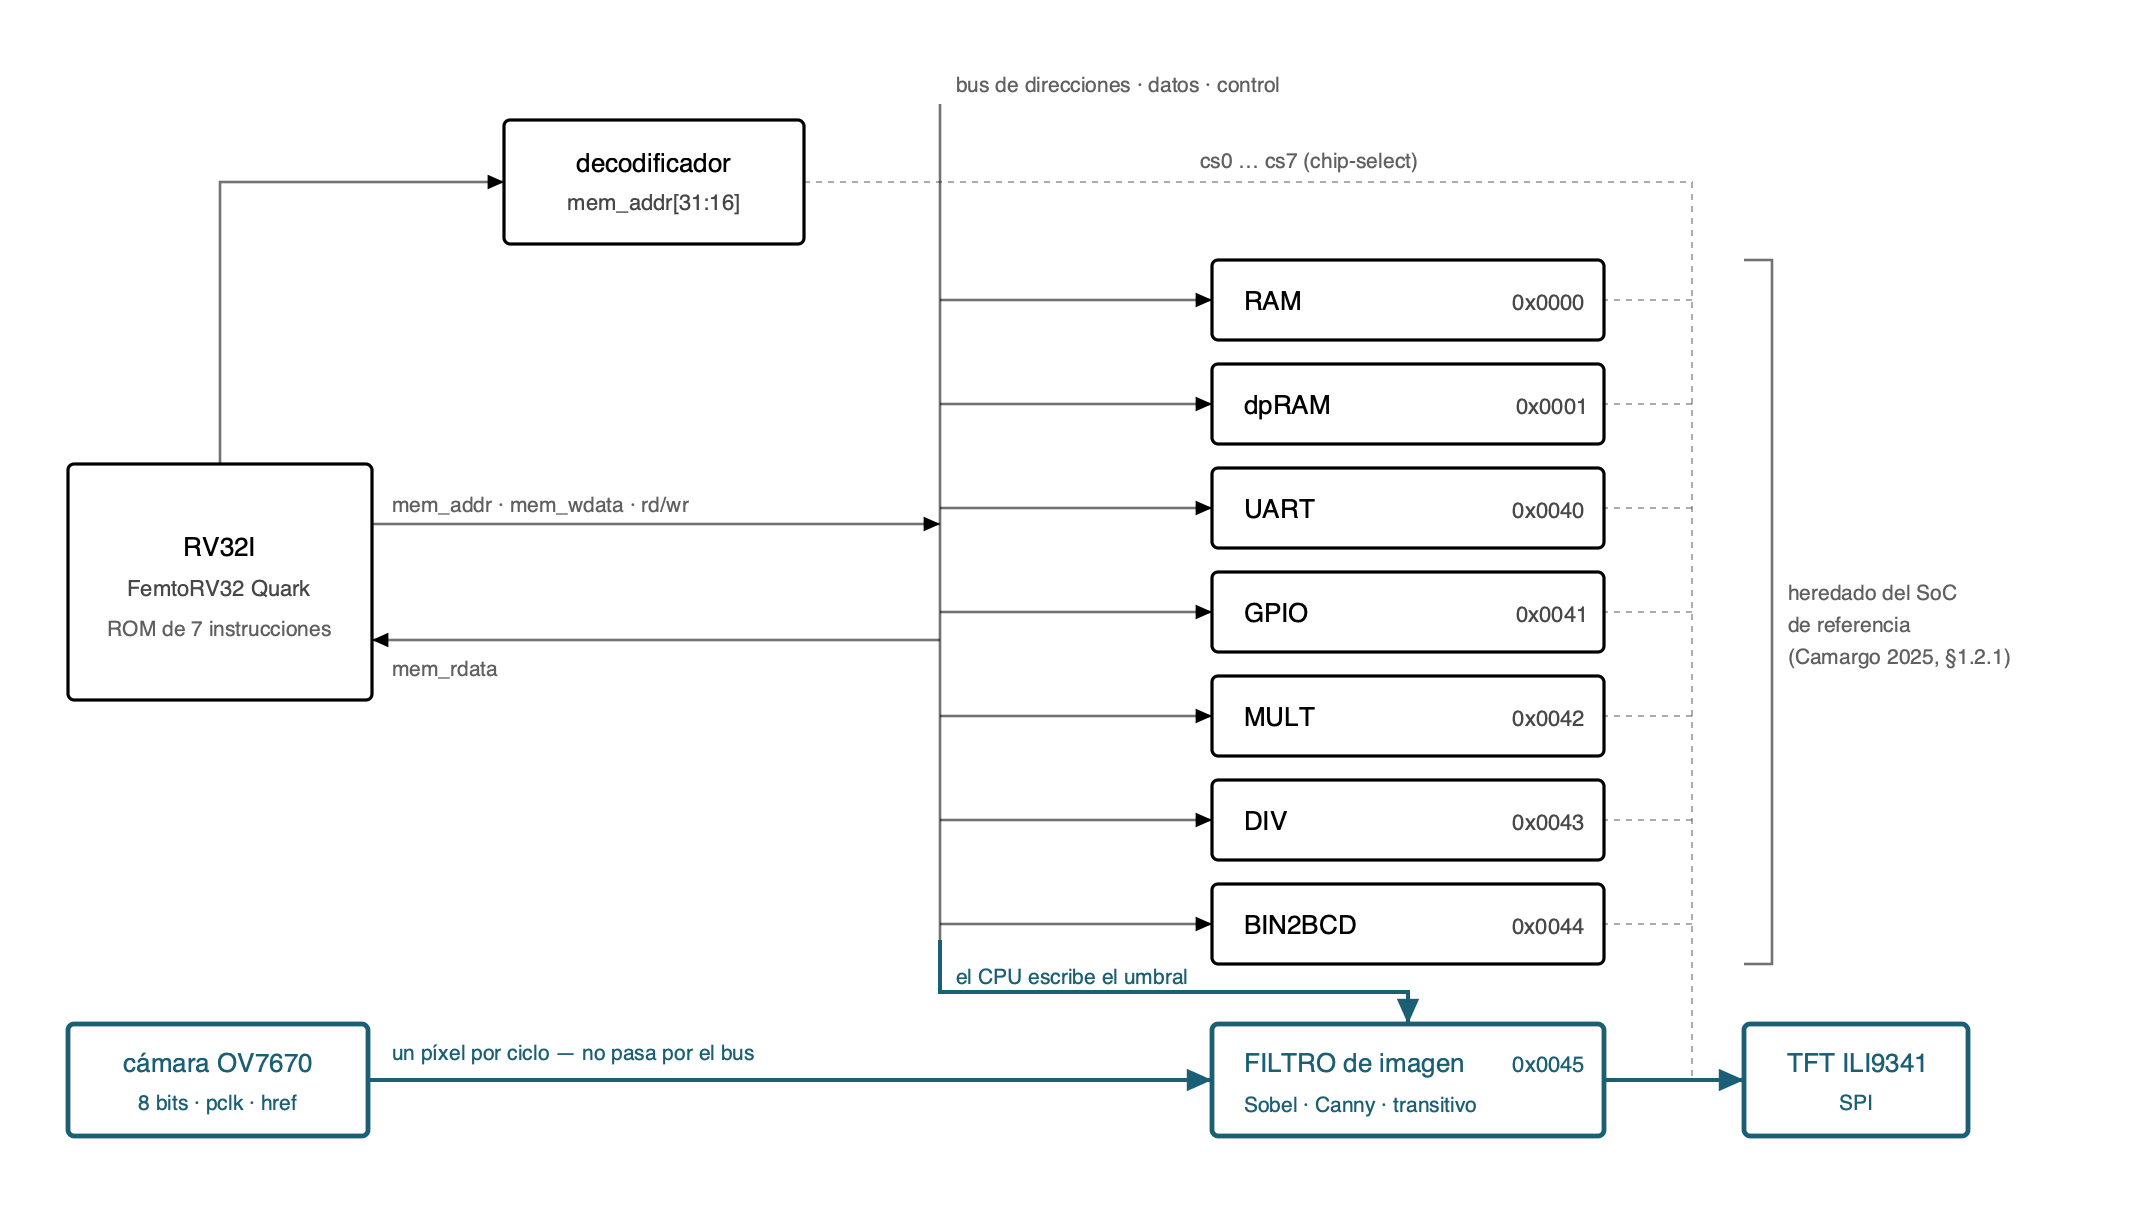
\includegraphics[keepaspectratio,alt={Figura 4.1. El sistema en silicio, en el lenguaje de bloques del SoC de referencia. Los siete periféricos en gris son los heredados; el que aparece destacado, en la base 0x0045, es la aportación de este trabajo. Obsérvese que el camino de datos de imagen no pasa por el bus: los píxeles entran de la cámara al filtro y salen de éste a la pantalla a un píxel por ciclo, y lo único que el procesador pone en el bus es el umbral.}]{figuras/fig_4_1_soc.png}}
\caption{\textbf{Figura 4.1.} El sistema en silicio, en el lenguaje de
bloques del SoC de referencia. Los siete periféricos en gris son los
heredados; el que aparece destacado, en la base \texttt{0x0045}, es la
aportación de este trabajo. Obsérvese que \textbf{el camino de datos de
imagen no pasa por el bus}: los píxeles entran de la cámara al filtro y
salen de éste a la pantalla a un píxel por ciclo, y lo único que el
procesador pone en el bus es el umbral.}
\end{figure}

La figura muestra por qué este periférico no se parece a los demás. Un
multiplicador o un divisor reciben sus operandos por el bus y devuelven
el resultado por el bus: el procesador los usa. El filtro, en cambio,
\textbf{tiene su propio camino de datos} ---de la cámara a la pantalla,
a un píxel por ciclo--- y del bus recibe únicamente un parámetro de
configuración. El procesador no lo usa: lo \textbf{ajusta}.

\begin{quote}
Esa distinción es la que el Capítulo 6 convierte en argumento. Un
periférico que procesa a través del bus está limitado por el ancho de
banda del bus; uno que procesa al margen de él, no. Es la razón de que
un sistema de visión en tiempo real pueda construirse sobre un
procesador de siete instrucciones.
\end{quote}

El firmware ocupa \textbf{siete instrucciones}: inicializa, escribe el
umbral y queda en un lazo. No es un programa modesto por limitación sino
por diseño --- el procesador existe para poder cambiar un parámetro en
tiempo de ejecución, no para procesar.

\subsection{La ROM sintetizada}\label{la-rom-sintetizada}

En una FPGA el contenido de la memoria de programa se carga con el
\emph{bitstream}. \textbf{En un ASIC no hay nada que lo cargue}: los
biestables arrancan en un estado indefinido. La memoria de programa debe
por tanto sintetizarse como lógica combinacional ---una tabla de
constantes--- y no como un arreglo inicializado.

Es el primero de los cuatro cambios obligatorios de la §4.8, y el que
más sorprende a quien llega desde FPGA, porque el código funciona
idénticamente en simulación en ambos casos.

\section{4.6 Memoria: la batalla de los
recursos}\label{memoria-la-batalla-de-los-recursos}

La iCE40UP5K ofrece tres clases de almacenamiento, y el diseño usa las
tres con criterios distintos:

\begin{longtable}[]{@{}
  >{\raggedright\arraybackslash}p{(\linewidth - 4\tabcolsep) * \real{0.3333}}
  >{\raggedright\arraybackslash}p{(\linewidth - 4\tabcolsep) * \real{0.3333}}
  >{\raggedright\arraybackslash}p{(\linewidth - 4\tabcolsep) * \real{0.3333}}@{}}
\toprule\noalign{}
\begin{minipage}[b]{\linewidth}\raggedright
Recurso
\end{minipage} & \begin{minipage}[b]{\linewidth}\raggedright
Cantidad
\end{minipage} & \begin{minipage}[b]{\linewidth}\raggedright
Uso en este trabajo
\end{minipage} \\
\midrule\noalign{}
\endhead
\bottomrule\noalign{}
\endlastfoot
Celdas lógicas & 5 280 & lógica y registros pequeños \\
Bloques de memoria (4 kbit) & 30 & \textbf{memorias de línea} de las
ventanas 3×3 \\
SPRAM (256 kbit) & 4 & \textbf{framebuffers} del filtro transitivo \\
\end{longtable}

La asignación no es libre: una memoria de línea cabe en un bloque de
memoria si el sintetizador la reconoce como tal, y no la reconoce si el
código la escribe de una forma que no encaja con el patrón esperado.
Varios de los problemas de recursos del desarrollo fueron de esa
naturaleza ---memorias que se convertían en biestables por un detalle de
escritura del RTL--- y no de tamaño real del diseño.

El caso más costoso fue un \textbf{ancho de puntero insuficiente}: un
contador de direcciones con un bit de menos del necesario direcciona la
mitad de la memoria y sobrescribe la otra, produciendo una imagen que se
ve plausible pero está mal. Como en el caso del byte de luminancia, el
error sobrevive a la inspección visual.

\begin{quote}
Este apartado es el origen del título del Capítulo 6. En la FPGA los dos
primeros recursos parecen gratuitos porque ya están en el sustrato; en
el ASIC ninguno lo es, y el mismo RTL que allí cabía holgadamente aquí
define el tamaño del dado.
\end{quote}

\section{4.7 Del RTL a la FPGA}\label{del-rtl-a-la-fpga}

El camino a la FPGA impuso sus propias decisiones.

\textbf{El intercambio entre celdas lógicas y bloques de memoria.}
Forzar más memorias de línea a bloques libera celdas pero consume
bloques, que son treinta. En varios puntos del desarrollo el diseño
estuvo limitado alternativamente por uno y por otro, y la solución
consistió en mover recursos entre ambos hasta encontrar una combinación
que cerrara.

\textbf{El bug del cerrojo.} Una asignación condicional incompleta
dentro de un bloque combinacional infiere un cerrojo en lugar de lógica.
El diseño sintetiza, ocupa recursos parecidos y funciona en simulación;
en la placa produce un comportamiento dependiente de la temporización.
La herramienta lo advierte, y la advertencia es fácil de ignorar entre
otras muchas.

\textbf{El bring-up incremental.} El sistema se puso en marcha por
etapas, cada una verificable por sí misma: parpadeo, reloj,
configuración SCCB, imagen en gris, memorias de línea, filtro, umbral,
motor, procesador. La razón es que \textbf{cada etapa es el banco de
pruebas de la siguiente}: cuando el filtro no produjo imagen, disponer
de la etapa anterior funcionando permitió decidir en un solo intento si
el problema estaba en el filtro o en la captura.

\section{4.8 Del RTL al ASIC: los cuatro cambios
obligatorios}\label{del-rtl-al-asic-los-cuatro-cambios-obligatorios}

El mismo Verilog no sirve para los dos destinos. Cuatro cosas hay que
cambiar, y ninguna de ellas produce un error de simulación ---por eso
son peligrosas.

\textbf{1. La memoria de programa debe sintetizarse.} Ya explicado en la
§4.5: en silicio no existe el \emph{bitstream} que la inicializa.

\textbf{2. Reset explícito en todos los registros de control.} En una
FPGA los biestables arrancan en el valor que el \emph{bitstream} les da;
en silicio arrancan en un estado indefinido. Toda máquina de estados
necesita una señal de reinicio explícita, y omitirla produce un circuito
que en simulación arranca correctamente y en la mesa no arranca nunca.

\textbf{3. Fuera el tri-estado interno.} El bus de datos de la cámara es
bidireccional y en FPGA se describe con alta impedancia dentro del
diseño. Un ASIC de celda estándar no dispone de eso: la señal debe
partirse en un dato y un habilitador ---\texttt{cam\_sda\_o} y
\texttt{cam\_sda\_oe}--- y el tri-estado real ocurre en el anillo de
pads.

\textbf{4. Fuera las primitivas del fabricante.} Los bloques específicos
de Lattice ---el controlador del LED RGB, entre otros--- no existen en
sky130. Se sustituyen por pines ordinarios o se eliminan.

\begin{quote}
Los cuatro cambios comparten una propiedad que conviene subrayar:
\textbf{ninguno produce un fallo visible en simulación RTL}. Un diseño
con \texttt{initial} heredado de FPGA simula perfectamente y sale de
fábrica mudo. Los dos únicos que se detectaron a tiempo durante este
trabajo aparecieron en \textbf{simulación de compuertas}, después de la
síntesis, y no antes.
\end{quote}

\chapter{5. Resultados}\label{resultados}

\section{5.1 Verificación funcional}\label{verificaciuxf3n-funcional}

\begin{quote}
\textbf{Estado:} borrador 1, escrito el 2026-09-16. Fuente: cuaderno 1,
Partes 29-35. Formato Markdown para convertir con \texttt{pandoc} a Word
o LaTeX según decida la guía de la Facultad.
\end{quote}

Antes de presentar área, frecuencia o consumo conviene establecer que
los circuitos \textbf{calculan lo que deben calcular}. Esta sección lo
hace, y distingue con cuidado dos preguntas que la literatura de
implementación mezcla con frecuencia: si el hardware coincide con su
modelo de referencia, y si el resultado es bueno. Aquí sólo se responde
la primera. La segunda pertenece a la §5.6.

\subsection{5.1.1 El criterio}\label{el-criterio}

Cada filtro se especificó primero como un programa en Python ---el
\textbf{modelo golden} descrito en la §3.2--- y sólo después se escribió
su descripción en Verilog. La verificación consiste en ejecutar ambos
sobre la misma entrada y comparar \textbf{píxel a píxel}, no en
inspeccionar visualmente la salida.

La distinción no es formal. Un mapa de bordes erróneo sigue pareciendo
un mapa de bordes, de modo que la inspección visual no distingue un
circuito correcto de uno que desplaza una fila, satura un byte o
invierte un signo. Sólo la comparación numérica lo hace.

Al comparar se admite un \textbf{desplazamiento constante} entre ambas
salidas ---la técnica de \emph{best-shift} de la §3.3--- porque la
implementación en hardware introduce una latencia de segmentación que el
modelo en software no tiene. Un desfase uniforme de \emph{k} píxeles no
es un error de cálculo sino una propiedad de la arquitectura segmentada,
y se descuenta explícitamente; cualquier diferencia que sobreviva a esa
corrección sí lo es.

\subsection{5.1.2 Resultado sobre los núcleos
aislados}\label{resultado-sobre-los-nuxfacleos-aislados}

Los tres núcleos son \textbf{idénticos bit a bit} a su modelo de
referencia. En el caso del Sobel sobre un cuadro de 60×80, la
comparación arroja \textbf{0 píxeles de diferencia sobre 4 800}, y el
resultado se sostiene para los tres filtros sobre las cinco imágenes de
prueba.

\begin{longtable}[]{@{}lrrr@{}}
\toprule\noalign{}
Núcleo & Imágenes & Píxeles comparados & Diferencias \\
\midrule\noalign{}
\endhead
\bottomrule\noalign{}
\endlastfoot
Sobel 3×3 & 5 / 5 & 4 800 por cuadro & \textbf{0} \\
Canny de un salto & 5 / 5 & 4 800 por cuadro & \textbf{0} \\
Canny transitivo & 5 / 5 & 4 800 por cuadro & \textbf{0} \\
\end{longtable}

Que la coincidencia sea exacta y no aproximada tiene una causa de
diseño: los tres filtros operan \textbf{sobre enteros y sin división}.
La magnitud del gradiente usa la norma L1,
\texttt{\textbar{}Gx\textbar{}+\textbar{}Gy\textbar{}}, en lugar de la
euclídea; los pesos del operador son potencias de dos, implementadas
como desplazamientos; y el umbral es una comparación. No hay ninguna
operación cuyo redondeo pueda diferir entre una biblioteca de punto
flotante y un circuito. \textbf{La igualdad bit a bit no es una
casualidad afortunada: es consecuencia de haber elegido una aritmética
que la permite.}

\subsection{5.1.3 Resultado sobre la cadena completa con
cámara}\label{resultado-sobre-la-cadena-completa-con-cuxe1mara}

La verificación anterior alimenta el circuito con una imagen almacenada.
La cadena real recibe en cambio un flujo de video de la cámara OV7670,
con sus bordes de línea, sus tiempos muertos y su sincronismo propio.
Medida sobre ese flujo, la concordancia entre el hardware y el modelo
es:

\begin{longtable}[]{@{}lr@{}}
\toprule\noalign{}
Cadena & Concordancia \\
\midrule\noalign{}
\endhead
\bottomrule\noalign{}
\endlastfoot
Sobel & 95 -- 100 \% \\
Canny de un salto & 88 -- 99 \% \\
Canny transitivo & 96 -- 100 \% \\
Promedio a través del SoC & \textbf{97,8 \%} \\
\end{longtable}

La degradación respecto del 100 \% de la §5.1.2 no proviene del filtro
sino del \textbf{acoplamiento con la cámara}: el muestreo del flujo, el
recorte de la ventana y el instante exacto en que empieza un cuadro
introducen diferencias de uno o dos píxeles en los bordes de la imagen.
El valor más bajo corresponde al Canny de un salto, que es también el
más sensible por construcción ---un píxel que cruza el umbral alto
propaga su decisión a sus vecinos, de modo que una diferencia aislada en
la entrada puede producir varias en la salida.

\begin{quote}
\textbf{Dos precisiones de terminología, porque el número se presta a
confusión.}

Primera: los porcentajes de esta tabla son \textbf{concordancia entre el
hardware y su propio modelo de referencia}, no exactitud del filtro.
Miden si el circuito hace lo que el programa hace, no si lo que el
programa hace es correcto o útil. Un filtro mal diseñado puede alcanzar
el 100 \% de concordancia con un modelo igualmente mal diseñado.

Segunda: la \textbf{densidad de bordes} ---la fracción de píxeles
marcados, en torno al 2 \% en las imágenes de prueba--- aparece en
varias figuras de este trabajo y \textbf{no es una medida de calidad}.
Es una propiedad de la escena y del punto de operación elegido, y su
valor «correcto» depende de para qué se vaya a usar el mapa de bordes.
La §5.6.4 muestra precisamente que mover ese punto de operación cambia
el resultado de clasificación más que cambiar de filtro.
\end{quote}

\section{5.2 Resultados en FPGA}\label{resultados-en-fpga}

\begin{quote}
\textbf{Estado:} borrador 2, 2026-09-21. Fuente: cuaderno 1, Partes
25-28 y 68-82, y los informes de \texttt{nextpnr-ice40} conservados de
las corridas del 30 de julio y del 3 de agosto de 2026.
\end{quote}

Los resultados de esta sección son de una clase distinta a los del resto
del capítulo: no provienen de un informe de herramienta sino de
\textbf{un circuito que funciona sobre una mesa}, con una cámara
apuntando a un objeto y una pantalla mostrando el resultado. Es la única
parte del trabajo donde el sistema completo existe físicamente, y por
eso condiciona lo que puede afirmarse de las demás.

\subsection{5.2.1 La plataforma}\label{la-plataforma}

La implementación física se realizó sobre una \textbf{iCE40UP5K} en
tarjeta iCESugar v1.5, con una cámara \textbf{OV7670} y una pantalla
\textbf{TFT ILI9341} por SPI. El flujo de síntesis e implementación es
enteramente abierto: \texttt{yosys} para síntesis,
\texttt{nextpnr-ice40} para emplazamiento y ruteo, \texttt{icepack} para
el \emph{bitstream}.

La elección del dispositivo no es incidental. La iCE40UP5K ofrece 5 280
celdas lógicas, 30 bloques de memoria de 4 kbit y \textbf{cuatro bloques
de SPRAM de 256 kbit} --- y son estos últimos los que hacen posible el
filtro transitivo, porque permiten alojar el cuadro completo sin
consumir lógica. Esa disponibilidad es exactamente lo que desaparece al
pasar a un ASIC sin macro de memoria, y es el origen del resultado de la
§5.4.3.

\subsection{5.2.2 Los tres filtros,
funcionando}\label{los-tres-filtros-funcionando}

\begin{longtable}[]{@{}
  >{\raggedright\arraybackslash}p{(\linewidth - 6\tabcolsep) * \real{0.2500}}
  >{\raggedright\arraybackslash}p{(\linewidth - 6\tabcolsep) * \real{0.2500}}
  >{\raggedright\arraybackslash}p{(\linewidth - 6\tabcolsep) * \real{0.2500}}
  >{\raggedright\arraybackslash}p{(\linewidth - 6\tabcolsep) * \real{0.2500}}@{}}
\toprule\noalign{}
\begin{minipage}[b]{\linewidth}\raggedright
Filtro
\end{minipage} & \begin{minipage}[b]{\linewidth}\raggedright
Arquitectura
\end{minipage} & \begin{minipage}[b]{\linewidth}\raggedright
Implementación física
\end{minipage} & \begin{minipage}[b]{\linewidth}\raggedright
Umbrales en la placa
\end{minipage} \\
\midrule\noalign{}
\endhead
\bottomrule\noalign{}
\endlastfoot
Sobel & flujo & hardware, con procesador FemtoRV32 & 90 \\
Canny de un salto & flujo & hardware, con procesador FemtoRV32 & 50 /
20 \\
Canny transitivo & \textbf{framebuffer} & hardware, motor en Verilog
\textbf{sin procesador} & 60 / 30 \\
\end{longtable}

Los tres funcionan sobre la placa con cámara y pantalla en vivo. El
transitivo produce contornos \textbf{conectados y completos} ---una
letra cerrada aparece cerrada--- frente a los bordes locales de los
otros dos, que es precisamente lo que su punto fijo debe conseguir.

\begin{figure}
\centering
\pandocbounded{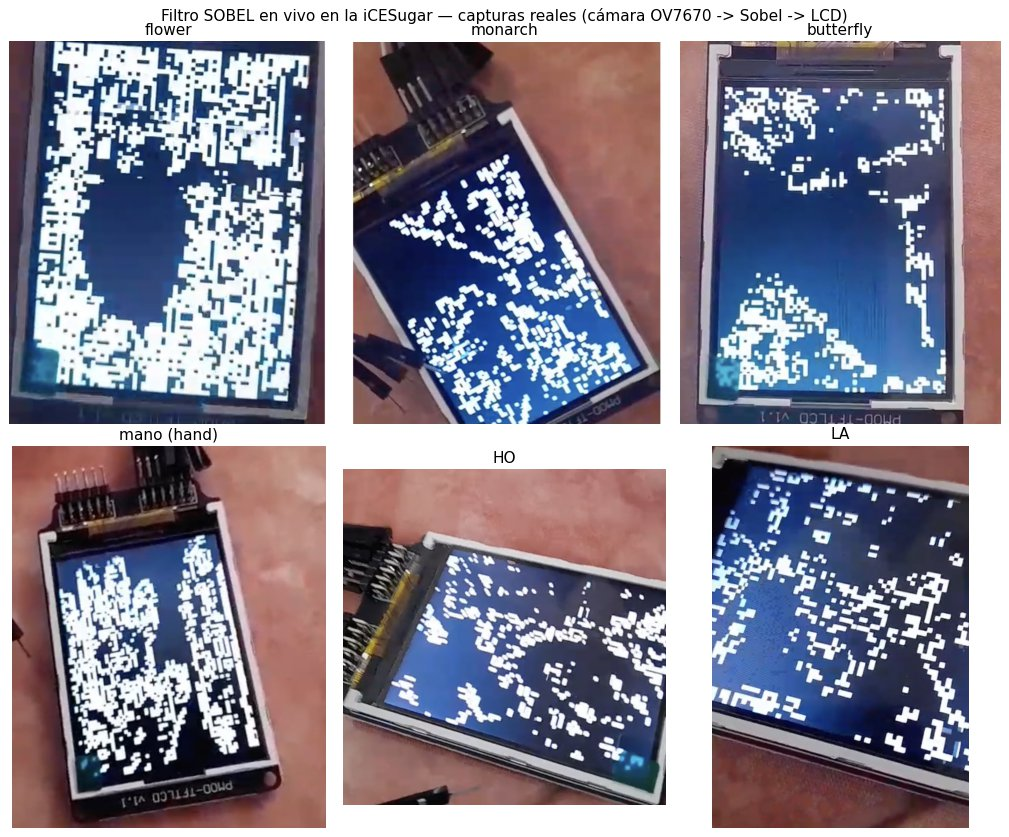
\includegraphics[keepaspectratio,alt={Figura 5.1. El filtro Sobel corriendo en vivo sobre la iCESugar, fotografiado directamente de la pantalla. Seis escenas distintas ---una flor, dos mariposas, una mano y dos letras--- recorren la cadena completa cámara → filtro → pantalla sin intervención de ningún computador. Son capturas del montaje físico, no reconstrucciones: la propia tarjeta y el cableado del módulo aparecen en el encuadre.}]{figuras/fig_5_1_sobel_en_vivo.jpg}}
\caption{\textbf{Figura 5.1.} El filtro Sobel corriendo en vivo sobre la
iCESugar, fotografiado directamente de la pantalla. Seis escenas
distintas ---una flor, dos mariposas, una mano y dos letras--- recorren
la cadena completa cámara → filtro → pantalla sin intervención de ningún
computador. Son capturas del montaje físico, no reconstrucciones: la
propia tarjeta y el cableado del módulo aparecen en el encuadre.}
\end{figure}

\subsection{5.2.3 Utilización del
dispositivo}\label{utilizaciuxf3n-del-dispositivo}

La tabla recoge el \textbf{Device utilisation} que informa
\texttt{nextpnr-ice40} tras el emplazamiento y ruteado
---\texttt{-\/-up5k\ -\/-package\ sg48}---, que es la medida
autoritativa: la que dice si el diseño entra en el dispositivo. Las
cinco filas de una misma columna proceden de \textbf{una sola corrida
con una sola versión de las herramientas}, para que sean comparables
entre sí.

\begin{longtable}[]{@{}
  >{\raggedright\arraybackslash}p{(\linewidth - 12\tabcolsep) * \real{0.1111}}
  >{\raggedleft\arraybackslash}p{(\linewidth - 12\tabcolsep) * \real{0.1481}}
  >{\raggedleft\arraybackslash}p{(\linewidth - 12\tabcolsep) * \real{0.1481}}
  >{\raggedleft\arraybackslash}p{(\linewidth - 12\tabcolsep) * \real{0.1481}}
  >{\raggedleft\arraybackslash}p{(\linewidth - 12\tabcolsep) * \real{0.1481}}
  >{\raggedleft\arraybackslash}p{(\linewidth - 12\tabcolsep) * \real{0.1481}}
  >{\raggedleft\arraybackslash}p{(\linewidth - 12\tabcolsep) * \real{0.1481}}@{}}
\toprule\noalign{}
\begin{minipage}[b]{\linewidth}\raggedright
Diseño
\end{minipage} & \begin{minipage}[b]{\linewidth}\raggedleft
LC / 5 280
\end{minipage} & \begin{minipage}[b]{\linewidth}\raggedleft
BRAM / 30
\end{minipage} & \begin{minipage}[b]{\linewidth}\raggedleft
SPRAM / 4
\end{minipage} & \begin{minipage}[b]{\linewidth}\raggedleft
E/S / 39
\end{minipage} & \begin{minipage}[b]{\linewidth}\raggedleft
\emph{f}máx sistema
\end{minipage} & \begin{minipage}[b]{\linewidth}\raggedleft
\emph{f}máx cámara
\end{minipage} \\
\midrule\noalign{}
\endhead
\bottomrule\noalign{}
\endlastfoot
Transitivo, motor dedicado \textbf{sin procesador} & 2 426 (45 \%) & 17
(56 \%) & \textbf{2 (50 \%)} & 18 (46 \%) & \textbf{28,7 MHz} ✓ & 20,6
MHz ✓ \\
SoC + Sobel & 4 848 (91 \%) & 20 (66 \%) & 0 & 18 (46 \%) & 9,5 MHz ✗ &
20,7 MHz ✓ \\
SoC + Canny de un salto & 5 234 (\textbf{99 \%}) & 24 (80 \%) & 0 & 18
(46 \%) & 9,5 MHz ✗ & 17,7 MHz ✓ \\
SoC + transitivo \textbf{por software} & 5 251 (\textbf{99 \%}) & 28 (93
\%) & 0 & 18 (46 \%) & 8,7 MHz ✗ & 20,5 MHz ✓ \\
SoC + transitivo \textbf{como periférico} & no emplaza (≈ 127 \%) & ---
& --- & --- & --- & --- \\
\end{longtable}

\begin{quote}
\textbf{Procedencia.} Las cuatro primeras filas se midieron de nuevo
para este documento. Tres de ellas ---las filas primera, tercera y
cuarta--- reprodujeron \textbf{exactamente}, celda por celda y bloque
por bloque, los informes conservados de las corridas originales de julio
y agosto de 2026. La del SoC + Sobel, cuyo informe de emplazamiento no
se había conservado, arrojó 4 848 celdas frente a las 4 878 anotadas
entonces en el cuaderno; la diferencia, de treinta celdas sobre cinco
mil, proviene de una versión distinta del sintetizador, que produce doce
tablas de consulta menos. La quinta fila no dispone de informe: el
emplazamiento no llegó a completarse, y el ≈ 127 \% es el valor
documentado en su momento.
\end{quote}

De la tabla se desprenden tres lecturas.

\textbf{La memoria grande sólo la usa un diseño.} Los cuatro bloques de
SPRAM ---256 kbit cada uno--- están sin tocar en todas las variantes de
flujo, y sólo el transitivo consume dos. Es coherente con su
arquitectura: es el único que necesita el cuadro entero a la vez. Los
filtros de flujo se las arreglan con dos filas de retardo, que caben en
los bloques de memoria pequeños.

\textbf{El límite de frecuencia lo pone el procesador, y no la
ocupación.} Los tres diseños que llevan el FemtoRV32 se agrupan entre
8,7 y 9,5 MHz mientras que el que no lo lleva alcanza 28,7 MHz:
\textbf{tres veces más rápido}. La tentación es atribuirlo a la
congestión ---los dos más lentos están al 99 \%---, pero la tabla lo
desmiente: el SoC del Sobel, \textbf{ocho puntos más vacío} que el del
Canny, cierra a la misma frecuencia, y de hecho una centésima por
debajo. La causa está en el informe de caminos críticos, que en los tres
SoC señala el mismo origen: \textbf{el registro de instrucción del
procesador}. El camino va de un flanco de subida a uno de bajada, de
modo que dispone de \textbf{medio período} en lugar de uno entero, y eso
divide por dos la frecuencia alcanzable. La síntesis lo confirma por
otra vía: los tres SoC contienen \textbf{2 048 biestables sensibles al
flanco de bajada} y el diseño sin procesador no contiene
\textbf{ninguno}. No es un problema de emplazamiento sino una propiedad
del procesador elegido, y es la razón de fondo de que las tres variantes
con CPU necesiten dividir el reloj.

\textbf{El sensor nunca fue el límite.} El dominio de la cámara cierra
con holgura en las cuatro filas medidas ---entre 17,7 y 20,7 MHz frente
a los 12 necesarios---, y es el del sistema el que falla. El cuello de
botella está del lado del procesamiento, no de la adquisición.

\begin{quote}
\textbf{Y una observación sobre el sustrato.} En los cuatro diseños el
retardo del camino crítico está dominado por el \textbf{ruteado}, que
aporta entre el 62 \% y el 72 \% del total; la lógica aporta el resto.
En una malla de interconexión fija como la de una FPGA esto es lo
esperable, y conviene tenerlo presente al leer la §5.4: en el ASIC,
donde el trazado se genera para el diseño concreto, ese reparto es otro.
\end{quote}

\subsection{5.2.4 El hallazgo de
co-diseño}\label{el-hallazgo-de-co-diseuxf1o}

El dato más importante de esta sección no es una cifra de utilización
sino una \textbf{decisión de arquitectura que la medida forzó}.

La intención inicial era que el procesador calculara la histéresis
transitiva por software, como hace en las versiones de los otros dos
filtros. Esa versión existe y funciona en simulación, con un 92,8 \% de
concordancia. Pero al intentar sintetizar el conjunto ---procesador,
memoria, framebuffers y motor--- la ocupación de celdas lógicas alcanzó
el \textbf{127 \%}: no cabía.

La respuesta fue mover el motor de histéresis de software a hardware,
como camino de datos en Verilog sin intervención del procesador. Así
implementado, la síntesis reporta \textbf{1 728 tablas de consulta} y el
emplazamiento \textbf{2 426 celdas lógicas, el 45 \% del dispositivo},
cerrando el temporizado a \textbf{28,7 MHz} con holgura.

\begin{quote}
Las dos cifras anteriores no son la misma medida, y conviene no
confundirlas: la celda lógica de la iCE40 empaqueta una tabla de
consulta \textbf{y} un biestable, de modo que un diseño con muchos
biestables sueltos ocupa más celdas que tablas tiene. Dividir el
recuento de tablas entre las 5 280 celdas del dispositivo da un 33 \%
que \textbf{subestima la ocupación real en doce puntos}. La cifra válida
es la del emplazamiento, no la de la síntesis; esta sección usa sólo la
primera.
\end{quote}

\begin{quote}
\textbf{Por qué esto es co-diseño y no una optimización.} No se trata de
que el hardware sea más rápido que el software, que es lo esperable. Se
trata de que \textbf{la restricción de recursos cambió el reparto de
responsabilidades entre las dos mitades del sistema}: la misma función,
expresada como programa, no cabía; expresada como circuito, ocupa un
tercio del dispositivo. La frontera entre lo que ejecuta el procesador y
lo que ejecuta la lógica dedicada no la fijó una preferencia de diseño
sino una medición.
\end{quote}

Este resultado reaparece transformado en la §5.4.2: en el ASIC, donde el
área no está acotada por un dispositivo fijo, el procesador vuelve a ser
viable junto al transitivo y cuesta unas nueve mil celdas. La misma
pregunta tiene respuestas opuestas en los dos sustratos.

\subsection{5.2.5 Umbrales de laboratorio y umbrales de
cámara}\label{umbrales-de-laboratorio-y-umbrales-de-cuxe1mara}

Las tres filas de la tabla anterior muestran umbrales distintos de los
que se usan en simulación. El transitivo, por ejemplo, pasó de 110/70 en
el banco de pruebas a \textbf{60/30 en la placa}.

El ajuste no es arbitrario ni es un defecto: una imagen almacenada y un
flujo de cámara tienen histogramas distintos, y el punto de operación
que extrae la estructura de una no es el que la extrae de la otra. La
§5.6.4 mide exactamente cuánto importa esa elección, y muestra que
\textbf{mover el umbral dentro de un filtro cambia el resultado de
clasificación más que cambiar de filtro}.

\begin{center}\rule{0.5\linewidth}{0.5pt}\end{center}

\begin{quote}
\textbf{Sobre la reproducibilidad de estas cifras.} Las cuatro filas
medidas se rehicieron el 21 de septiembre de 2026 con el guion
\texttt{medir\_utilizacion\_vm.sh}, que aplica a cada diseño las mismas
órdenes de lectura de fuentes que su guion de construcción original.
Tres de las cuatro reprodujeron el informe conservado sin desviarse en
una sola celda ni en un solo bloque de memoria, pese a mediar casi dos
meses entre una corrida y otra. La cuarta se desvió en treinta celdas
sobre cinco mil, y la causa está identificada: una versión distinta del
sintetizador. \textbf{El flujo es determinista a herramientas iguales},
que es lo que permite presentar estas cifras como medidas y no como
estimaciones.
\end{quote}

\section{5.3 Resultados en ASIC: los
bloques}\label{resultados-en-asic-los-bloques}

\begin{quote}
\textbf{Estado:} borrador 1, escrito el 2026-09-16. Fuente: cuaderno 1,
Partes 86-131, y el archivo de planos \texttt{ASIC\_planos/}.
\textbf{Recuento homogeneizado el 21 de septiembre de 2026.} Toda la
columna «celdas» de esta tabla son \textbf{celdas lógicas tras
emplazamiento y ruteado}, recontadas con un mismo criterio desde los
netlists archivados. Véase la §5.3.3 para cruzarlas con las de la §5.4.
\end{quote}

Esta sección presenta los circuitos que implementan \textbf{una función
cada uno}: los tres filtros por separado, los mismos con procesador, dos
bloques de interfaz y dos sistemas de visión. Son el vocabulario con el
que se construyen los sistemas de la §5.4, y su valor está en que
permiten atribuir el costo de cada pieza por separado.

Todos se llevaron a GDSII con \textbf{OpenLane} sobre el PDK abierto
\textbf{sky130A}, biblioteca \texttt{sky130\_fd\_sc\_hd}.

\subsection{5.3.1 La tabla}\label{la-tabla}

\begin{longtable}[]{@{}
  >{\raggedright\arraybackslash}p{(\linewidth - 8\tabcolsep) * \real{0.1765}}
  >{\raggedright\arraybackslash}p{(\linewidth - 8\tabcolsep) * \real{0.1765}}
  >{\raggedleft\arraybackslash}p{(\linewidth - 8\tabcolsep) * \real{0.2353}}
  >{\raggedleft\arraybackslash}p{(\linewidth - 8\tabcolsep) * \real{0.2353}}
  >{\centering\arraybackslash}p{(\linewidth - 8\tabcolsep) * \real{0.1765}}@{}}
\toprule\noalign{}
\begin{minipage}[b]{\linewidth}\raggedright
Circuito
\end{minipage} & \begin{minipage}[b]{\linewidth}\raggedright
Función
\end{minipage} & \begin{minipage}[b]{\linewidth}\raggedleft
Área del die
\end{minipage} & \begin{minipage}[b]{\linewidth}\raggedleft
Celdas
\end{minipage} & \begin{minipage}[b]{\linewidth}\centering
Signoff
\end{minipage} \\
\midrule\noalign{}
\endhead
\bottomrule\noalign{}
\endlastfoot
\texttt{sobel} & filtro Sobel 3×3 & 0,167 mm² & 5 823 & DRC/LVS/XOR =
0 \\
\texttt{canny1} & Canny de un salto, en flujo & 0,360 mm² & 12 993 &
DRC/LVS/XOR = 0 \\
\texttt{transitivo} & Canny con histéresis transitiva & 3,13 mm² & 65
659 & DRC/LVS/XOR = 0 \\
\texttt{soc\_sobel} & FemtoRV32 + Sobel & 0,37 mm² & 12 043 &
DRC/LVS/XOR = 0 \\
\texttt{soc\_canny1} & FemtoRV32 + Canny de un salto & 0,67 mm² & 22 054
& DRC/LVS/XOR = 0 \\
\texttt{soc\_trans} & FemtoRV32 + transitivo & 3,42 mm² & 72 337 &
DRC/LVS/XOR = 0 \\
\texttt{cam\_frontend} & front-end de cámara OV7670 & 0,0177 mm² & 562 &
DRC/LVS/XOR = 0 \\
\texttt{lcd\_ili9341} & driver de pantalla TFT por SPI & 0,0174 mm² &
553 & DRC/LVS/XOR = 0 \\
\texttt{vision\_top} & cámara + Sobel + framebuffer + pantalla & 1,75
mm² & 35 653 & DRC/LVS/XOR = 0 \\
\texttt{vision\_canny} & cámara + Canny + framebuffer + pantalla & 2,04
mm² & 41 925 & DRC/LVS/XOR = 0 \\
\end{longtable}

\textbf{Diez circuitos, diez veces DRC, LVS y XOR en cero.}

\subsection{5.3.2 Lo que la tabla muestra de un
vistazo}\label{lo-que-la-tabla-muestra-de-un-vistazo}

\textbf{El filtro transitivo cuesta casi veinte veces más área que el
Sobel} ---3,13 mm² contra 0,167, y once veces más celdas--- pese a
ejecutar aritmética comparable. La razón, ya anticipada, es el cuadro
completo residente: en la FPGA ese cuadro vivía en SPRAM y no consumía
lógica; aquí es un banco de biestables.

\textbf{Los dos bloques de interfaz son casi gratis.} El front-end de
cámara y el driver de pantalla ocupan menos de dieciocho milésimas de
milímetro cuadrado cada uno, alrededor de 560 celdas. Conviene tenerlo
medido porque desmonta una intuición común: el costo de un sistema de
visión embebido no está en hablar con los periféricos, está en lo que se
hace con los datos entre medias.

\begin{figure}
\centering
\pandocbounded{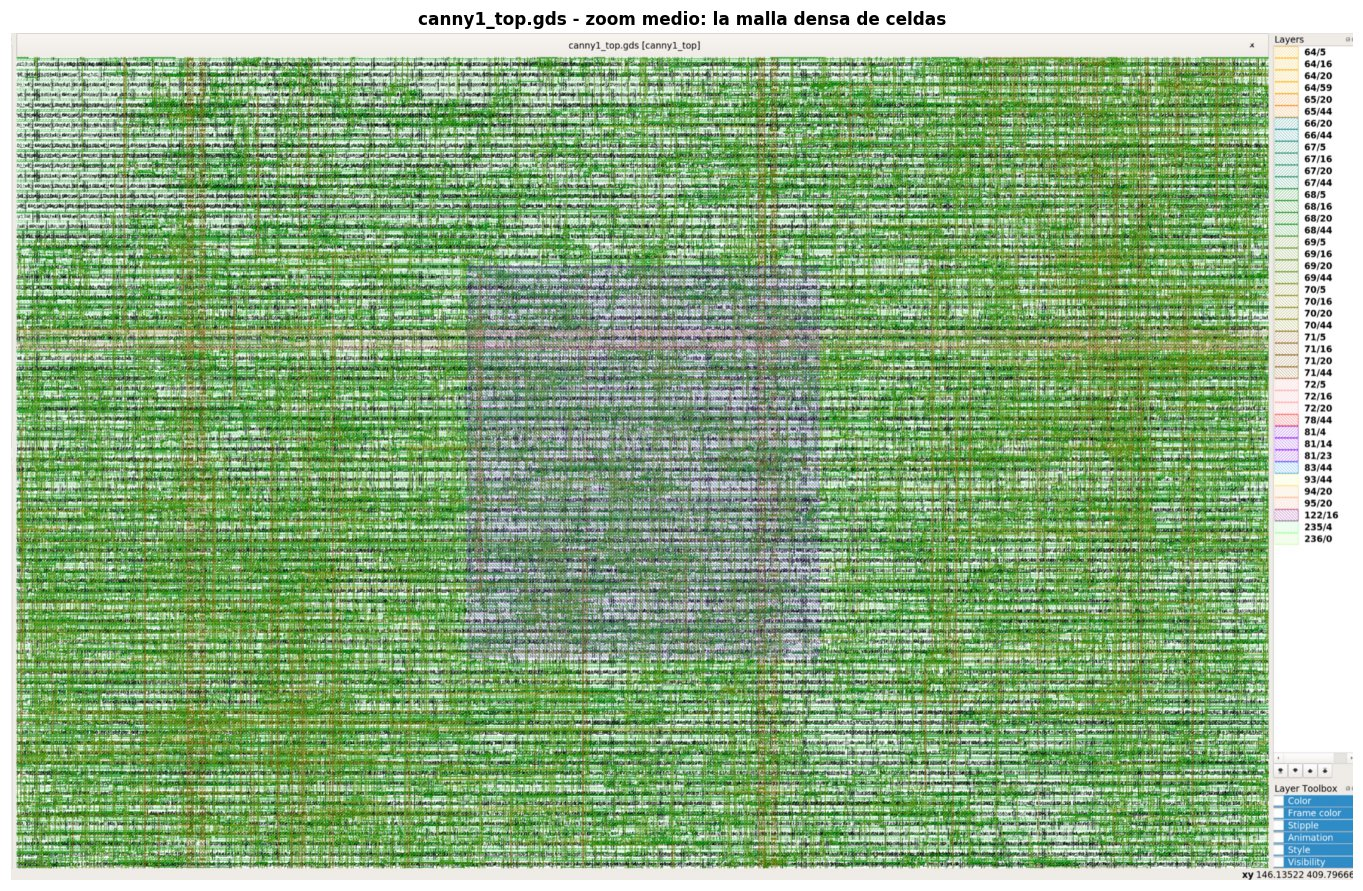
\includegraphics[keepaspectratio,alt={Figura 5.2. Acercamiento al GDSII del canny1 en KLayout. Lo que se ve no es un esquema sino el plano que iría a fábrica: filas de celdas estándar y, sobre ellas, las capas de metal que las conectan. La mancha más clara del centro es una región de menor densidad de ruteo. Las 12 993 celdas de la tabla anterior son, literalmente, estas.}]{figuras/fig_5_2_malla_canny1.jpg}}
\caption{\textbf{Figura 5.2.} Acercamiento al GDSII del \texttt{canny1}
en KLayout. Lo que se ve no es un esquema sino el plano que iría a
fábrica: filas de celdas estándar y, sobre ellas, las capas de metal que
las conectan. La mancha más clara del centro es una región de menor
densidad de ruteo. Las 12 993 celdas de la tabla anterior son,
literalmente, estas.}
\end{figure}

\textbf{Y el Sobel en silicio es mucho más rápido de lo que la FPGA
permitía.} Su camino crítico quedó en \textbf{7,69 ns} frente a un
objetivo de 20 ns, es decir que soportaría unos 130 MHz, mientras que en
la iCE40 cerraba entre 9 y 28 MHz. En silicio la lógica es rápida;
\textbf{lo caro es el área}, y ése es el eje sobre el que gira todo este
capítulo.

\subsection{5.3.3 El recuento de celdas, y cómo cruzar las dos
tablas}\label{el-recuento-de-celdas-y-cuxf3mo-cruzar-las-dos-tablas}

Esta advertencia no es un tecnicismo: afecta a cualquier comparación que
un lector intente hacer entre esta tabla y la de la §5.4.

Un circuito se puede contar en dos momentos del flujo, y las dos cifras
son legítimas:

\begin{longtable}[]{@{}
  >{\raggedright\arraybackslash}p{(\linewidth - 4\tabcolsep) * \real{0.3333}}
  >{\raggedright\arraybackslash}p{(\linewidth - 4\tabcolsep) * \real{0.3333}}
  >{\raggedright\arraybackslash}p{(\linewidth - 4\tabcolsep) * \real{0.3333}}@{}}
\toprule\noalign{}
\begin{minipage}[b]{\linewidth}\raggedright
Definición
\end{minipage} & \begin{minipage}[b]{\linewidth}\raggedright
Qué cuenta
\end{minipage} & \begin{minipage}[b]{\linewidth}\raggedright
Dónde se usa
\end{minipage} \\
\midrule\noalign{}
\endhead
\bottomrule\noalign{}
\endlastfoot
celdas de \textbf{síntesis} & el resultado de traducir el RTL a
compuertas & la tabla de la §5.4 \\
celdas \textbf{emplazadas} & lo que queda tras emplazar y rutear, con
los amortiguadores que el flujo inserta para el árbol de reloj y la
reparación de tiempos & \textbf{esta} tabla y la §5.6 \\
\end{longtable}

Durante la redacción, la columna «celdas» de este capítulo
\textbf{mezclaba las dos}, porque las fichas del cuaderno habían
registrado en cada momento el campo que la herramienta ofrecía.
\textbf{Se rehízo el recuento}: se contaron las instancias de celda
estándar directamente sobre el \textbf{netlist posterior al ruteado} de
cada circuito archivado, descartando las celdas sin función lógica
---relleno, contactos de pozo, desacoplo y diodos de antena---, con un
único criterio para los dieciséis.

El procedimiento se validó antes de aplicarlo: de los dieciséis
circuitos, \textbf{ocho reprodujeron exactamente la cifra que ya
constaba}, hasta la unidad ---los dos bloques de interfaz, los dos SoC,
los dos sistemas de visión y los dos circuitos en IHP---, que son
precisamente aquellos cuya ficha ya provenía del emplazamiento. Los ocho
restantes cambiaron, y ése era el objetivo.

\subsubsection{El factor de conversión,
medido}\label{el-factor-de-conversiuxf3n-medido}

Como en nueve circuitos se conservan las dos cifras, el paso de una a
otra no hay que estimarlo:

\begin{longtable}[]{@{}ll@{}}
\toprule\noalign{}
\endhead
\bottomrule\noalign{}
\endlastfoot
Casos medidos & 9 \\
Factor medio & \textbf{×1,21} \\
Mediana & ×1,20 \\
Rango & ×1,16 a ×1,26 \\
Desviación típica & 0,04 \\
\end{longtable}

\textbf{El emplazamiento agrega entre un 16 \% y un 26 \% de celdas},
con una dispersión estrecha. De modo que una cifra de la §5.4 se lleva a
la escala de ésta multiplicándola por 1,21, y el error de esa conversión
es de unos pocos puntos porcentuales --- no del 20 \% que separaba las
tablas antes de homogeneizarlas.

\begin{quote}
\textbf{Por qué no se convirtió también la §5.4.} Dos de sus seis
circuitos se archivaron sin netlist, de modo que convertir la tabla
habría exigido estimar dos de las seis filas. Se prefirió dejar cada
tabla \textbf{internamente homogénea} ---la §5.4 entera en celdas de
síntesis, ésta entera en celdas emplazadas--- y publicar el factor que
las relaciona, antes que producir una tabla mixta con dos filas
estimadas. Las comparaciones dentro de cada tabla son exactas; las que
cruzan de una a otra pasan por el factor.
\end{quote}

\section{5.4 Resultados en ASIC: la cadena de visión
completa}\label{resultados-en-asic-la-cadena-de-visiuxf3n-completa}

\begin{quote}
\textbf{Estado:} borrador 1, escrito el 2026-09-16. Fuente: cuaderno 1,
Partes 157-165, y la tabla maestra
\texttt{asic/tabla\_maestra/tabla\_6\_chips.py}, que la genera desde los
\texttt{metrics.csv} del flujo.
\end{quote}

La §5.3 presentó bloques: filtros solos, un front-end de cámara, un
driver de pantalla. Ésta presenta \textbf{sistemas}: seis circuitos que
llevan la cadena entera ---captura, filtrado, almacenamiento y
visualización--- en un solo dado. Los seis están organizados como una
matriz de dos variables, el \textbf{filtro} y la \textbf{presencia de
procesador}, de modo que cada comparación entre dos de ellos aísla una
sola causa.

\subsection{5.4.1 La tabla maestra}\label{la-tabla-maestra}

\begin{longtable}[]{@{}
  >{\raggedright\arraybackslash}p{(\linewidth - 20\tabcolsep) * \real{0.0811}}
  >{\raggedright\arraybackslash}p{(\linewidth - 20\tabcolsep) * \real{0.0811}}
  >{\raggedright\arraybackslash}p{(\linewidth - 20\tabcolsep) * \real{0.0811}}
  >{\centering\arraybackslash}p{(\linewidth - 20\tabcolsep) * \real{0.0811}}
  >{\raggedleft\arraybackslash}p{(\linewidth - 20\tabcolsep) * \real{0.1081}}
  >{\raggedleft\arraybackslash}p{(\linewidth - 20\tabcolsep) * \real{0.1081}}
  >{\raggedleft\arraybackslash}p{(\linewidth - 20\tabcolsep) * \real{0.1081}}
  >{\raggedleft\arraybackslash}p{(\linewidth - 20\tabcolsep) * \real{0.1081}}
  >{\centering\arraybackslash}p{(\linewidth - 20\tabcolsep) * \real{0.0811}}
  >{\centering\arraybackslash}p{(\linewidth - 20\tabcolsep) * \real{0.0811}}
  >{\centering\arraybackslash}p{(\linewidth - 20\tabcolsep) * \real{0.0811}}@{}}
\toprule\noalign{}
\begin{minipage}[b]{\linewidth}\raggedright
\#
\end{minipage} & \begin{minipage}[b]{\linewidth}\raggedright
Chip
\end{minipage} & \begin{minipage}[b]{\linewidth}\raggedright
Filtro
\end{minipage} & \begin{minipage}[b]{\linewidth}\centering
CPU
\end{minipage} & \begin{minipage}[b]{\linewidth}\raggedleft
Área (mm²)
\end{minipage} & \begin{minipage}[b]{\linewidth}\raggedleft
Celdas
\end{minipage} & \begin{minipage}[b]{\linewidth}\raggedleft
Reloj de firma
\end{minipage} & \begin{minipage}[b]{\linewidth}\raggedleft
Setup c/parásitos
\end{minipage} & \begin{minipage}[b]{\linewidth}\centering
DRC
\end{minipage} & \begin{minipage}[b]{\linewidth}\centering
LVS
\end{minipage} & \begin{minipage}[b]{\linewidth}\centering
XOR
\end{minipage} \\
\midrule\noalign{}
\endhead
\bottomrule\noalign{}
\endlastfoot
\#1 & \texttt{sobel\_completo} ᵃ & Sobel & --- & 2,45 & 36 730 & 20 ns
(50,0 MHz) & sin dato ᵇ & 0 & 0 & 0 \\
\#2 & \texttt{canny1\_completo} ᵃ & Canny1 & --- & 2,90 & 42 581 & 20 ns
(50,0 MHz) & sin dato ᵇ & 0 & 0 & 0 \\
\#3 & \texttt{trans\_completo} & Transitivo & --- & 9,61 & 137 092 & 20
ns (50,0 MHz) & \textbf{−19,35 ns} & 0 & 0 & 0 \\
\#4 & \texttt{soc\_sobel\_completo} & Sobel & ✓ & 3,03 & 46 019 & 32 ns
(31,2 MHz) & \textbf{+0,00 ns} & 0 & 0 & 0 \\
\#5 & \texttt{soc\_canny1\_completo} & Canny1 & ✓ & 3,44 & 51 037 & 36
ns (27,8 MHz) & \textbf{+0,00 ns} & 0 & 0 & 0 \\
\#6 & \texttt{soc\_trans\_completo} & Transitivo & ✓ & 10,19 & 146 216 &
36 ns (27,8 MHz) & \textbf{−18,23 ns} & 0 & 0 & 0 \\
\end{longtable}

ᵃ Estos dos se archivaron sin el directorio de reportes; sus cifras
provienen de la ficha del cuaderno y no de un \texttt{metrics.csv} del
flujo. Se marcan porque en una tabla de resultados debe poder decirse de
dónde sale cada número.

ᵇ Su ficha registra el \textbf{WNS nominal} ---0,00 ns, sin
violaciones--- pero no quedó registrado el setup ya con parásitos
extraídos, que es justamente la columna que hunde a los dos transitivos.
Se deja en blanco antes que suponer que cierran.

\textbf{Los seis llegaron a GDSII con DRC, LVS y XOR en cero.} Cuatro
cierran temporizado o carecen del dato para afirmar lo contrario; los
dos transitivos no cierran, y conviene decirlo con el número: el \#3
pediría 39,4 ns ---25,4 MHz--- y el \#6, 54,2 ns, es decir 18,4 MHz en
lugar de los 27,8 solicitados.

\begin{quote}
\textbf{Sobre el recuento de celdas, y es importante al leer junto a la
§5.3.} Las cifras de esta tabla son \textbf{celdas de síntesis}; las de
la §5.3 y la §5.6 son \textbf{celdas emplazadas}. Cada tabla es
internamente homogénea, y el paso de una escala a otra \textbf{está
medido sobre nueve circuitos que conservan las dos cifras}: el
emplazamiento agrega entre un 16 \% y un 26 \%, con un factor medio de
\textbf{×1,21} y una desviación típica de 0,04. Para comparar una cifra
de aquí con una de allá, multiplíquese por 1,21; el detalle del
procedimiento está en la §5.3.3.

Dos de los seis circuitos de esta tabla se archivaron sin
\emph{netlist}, razón por la cual no se convirtió la tabla entera: se
prefirió una tabla homogénea en su propia escala antes que una tabla
mixta con dos filas estimadas.
\end{quote}

\begin{figure}
\centering
\pandocbounded{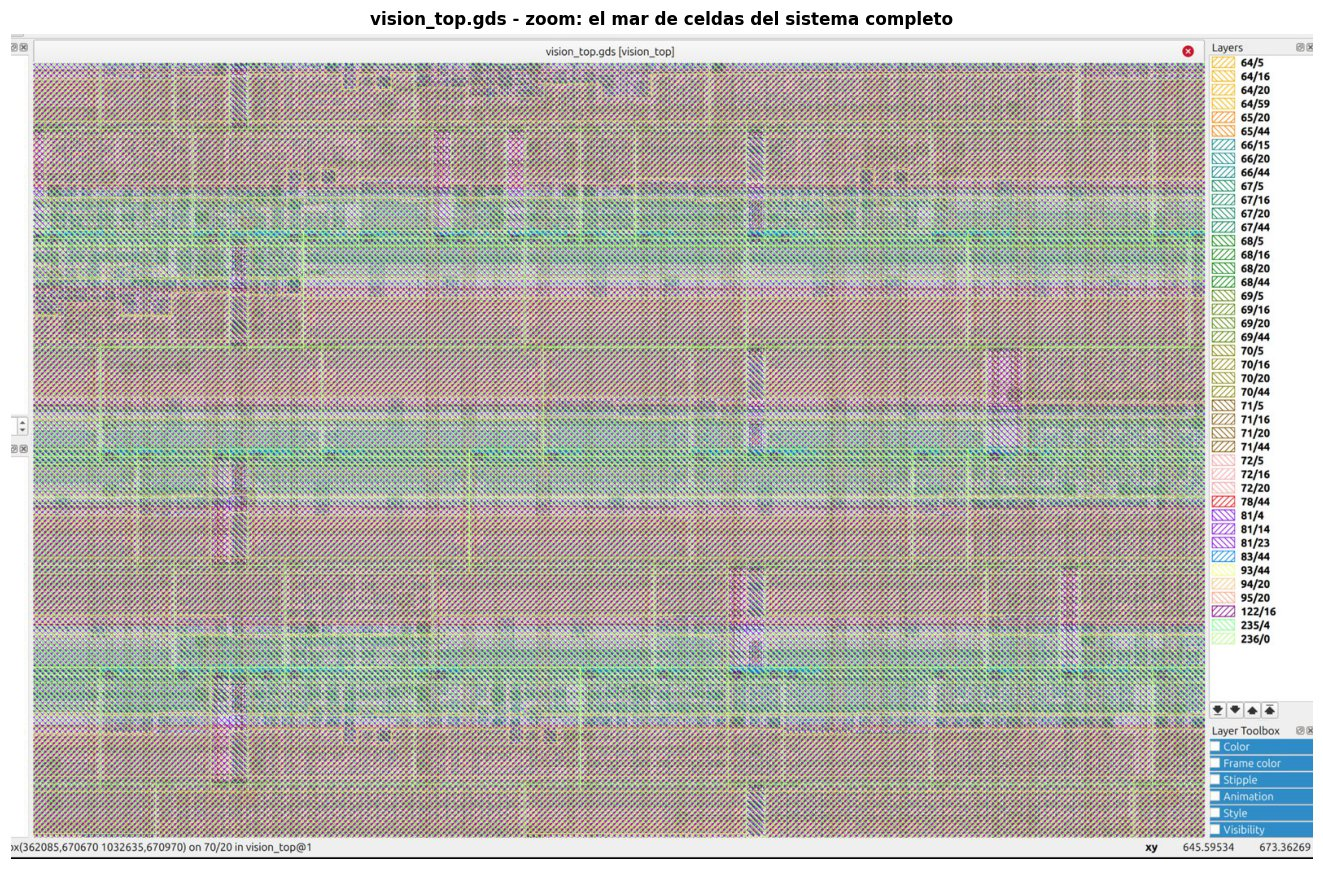
\includegraphics[keepaspectratio,alt={Figura 5.3. El mismo tipo de acercamiento, ahora sobre el sistema de visión completo. La diferencia con la figura anterior no está en la textura sino en la escala: aquí caben cámara, filtro, memoria de cuadro y controlador de pantalla en el mismo dado. Es la forma que toma en silicio la frase «el filtro es una pieza y no el circuito».}]{figuras/fig_5_3_mar_de_celdas_vision.jpg}}
\caption{\textbf{Figura 5.3.} El mismo tipo de acercamiento, ahora sobre
el sistema de visión completo. La diferencia con la figura anterior no
está en la textura sino en la escala: aquí caben cámara, filtro, memoria
de cuadro y controlador de pantalla en el mismo dado. Es la forma que
toma en silicio la frase «el filtro es una pieza y no el circuito».}
\end{figure}

\subsection{5.4.2 El procesador cuesta lo mismo, sea cual sea el
filtro}\label{el-procesador-cuesta-lo-mismo-sea-cual-sea-el-filtro}

Restando cada chip de su gemelo con procesador se obtiene el costo del
FemtoRV32, su memoria de programa y su periférico:

\begin{longtable}[]{@{}lrrrr@{}}
\toprule\noalign{}
Filtro & sin CPU & con CPU & Δ celdas & Δ relativo \\
\midrule\noalign{}
\endhead
\bottomrule\noalign{}
\endlastfoot
Sobel & 36 730 & 46 019 & \textbf{+9 289} & +25,3 \% \\
Canny de un salto & 42 581 & 51 037 & \textbf{+8 456} & +19,9 \% \\
Canny transitivo & 137 092 & 146 216 & \textbf{+9 124} & +6,7 \% \\
\end{longtable}

El incremento absoluto es \textbf{prácticamente constante}: alrededor de
nueve mil celdas, con una dispersión inferior al 5 \% entre el caso más
barato y el más caro. Es un resultado esperable ---el procesador no sabe
qué filtro tiene al lado--- pero conviene tenerlo medido, porque
convierte al procesador en un \textbf{costo fijo y presupuestable}
frente a un datapath cuyo costo varía en un factor de cuatro.

La columna relativa dice lo contrario que la absoluta, y las dos son
ciertas: el mismo procesador representa una cuarta parte del chip más
pequeño y apenas una quinceava parte del más grande. Cuál de las dos
lecturas importa depende de la pregunta. Para decidir si añadir un
procesador a un diseño dado, manda la absoluta.

\subsection{5.4.3 Lo que de verdad cuesta caro no es el cerebro: es la
memoria}\label{lo-que-de-verdad-cuesta-caro-no-es-el-cerebro-es-la-memoria}

El mismo ejercicio, hecho ahora sobre el eje del filtro en lugar del
procesador, produce el resultado central de este capítulo:

\begin{longtable}[]{@{}
  >{\raggedright\arraybackslash}p{(\linewidth - 6\tabcolsep) * \real{0.2143}}
  >{\raggedright\arraybackslash}p{(\linewidth - 6\tabcolsep) * \real{0.2143}}
  >{\raggedleft\arraybackslash}p{(\linewidth - 6\tabcolsep) * \real{0.2857}}
  >{\raggedleft\arraybackslash}p{(\linewidth - 6\tabcolsep) * \real{0.2857}}@{}}
\toprule\noalign{}
\begin{minipage}[b]{\linewidth}\raggedright
Alcance del patrón
\end{minipage} & \begin{minipage}[b]{\linewidth}\raggedright
Filtro
\end{minipage} & \begin{minipage}[b]{\linewidth}\raggedleft
Celdas (sin CPU)
\end{minipage} & \begin{minipage}[b]{\linewidth}\raggedleft
Δ respecto al anterior
\end{minipage} \\
\midrule\noalign{}
\endhead
\bottomrule\noalign{}
\endlastfoot
local, ventana 3×3 & Sobel & 36 730 & --- \\
local más un salto & Canny de un salto & 42 581 & +5 851 \\
\textbf{global, cuadro completo} & Canny transitivo & \textbf{137 092} &
\textbf{+94 511} \\
\end{longtable}

Pasar de mirar una ventana de 3×3 a mirar un salto más cuesta menos de
seis mil celdas. Pasar de ahí a \textbf{mirar el cuadro entero} cuesta
noventa y cuatro mil quinientas once.

La comparación directa es la que conviene enunciar: \textbf{un
procesador RISC-V completo, con su memoria y su periférico, pesa
aproximadamente la décima parte de lo que pesa cambiar el alcance del
patrón de local a global.} Nueve mil celdas contra noventa y cuatro mil
quinientas.

Y la razón no está en la aritmética. Los tres filtros ejecutan
esencialmente las mismas operaciones sobre cada píxel; lo que cambia es
\textbf{cuánto estado hay que sostener simultáneamente}. El Sobel y el
Canny de un salto procesan en flujo y necesitan unas pocas líneas de la
imagen ---los \emph{line-buffers} de la §4.6---, mientras que la
histéresis transitiva necesita el cuadro completo residente y accesible
en cualquier orden, porque su punto fijo puede propagar una decisión
desde cualquier píxel hacia cualquier otro. En una FPGA ese cuadro es un
bloque de memoria que ya está en el sustrato; en un ASIC sin macro de
memoria es un banco de biestables, y se paga en área, en potencia y en
frecuencia.

\begin{quote}
Éste es, en una sola cifra, el argumento que el Capítulo 6 desarrolla:
\textbf{lo que decide si un algoritmo cabe en silicio no es su
complejidad aritmética sino su huella de memoria.} Los dos transitivos
son además los dos únicos chips de la tabla que no cierran temporizado,
lo que muestra que el precio de esa memoria no se cobra sólo en
milímetros cuadrados.
\end{quote}

\subsection{5.4.4 Balance}\label{balance}

Seis circuitos, 459 675 celdas en total, \textbf{seis de seis con DRC =
LVS = XOR = 0}. Dos cierran temporizado con parásitos extraídos, dos
carecen de ese dato por haberse archivado sin reportes, y dos no cierran
y se documentan con la frecuencia que sí soportarían.

Ninguno ha sido fabricado. La §5.6.1 describe la vía por la que podrían
serlo.

\section{5.5 Rendimiento: caudal y
latencia}\label{rendimiento-caudal-y-latencia}

\begin{quote}
\textbf{Estado:} borrador 2, 2026-09-21. Fuente: cuaderno 1, Partes
154-156, y la corrida de \texttt{tb\_latencia\_final.v} del 21 de
septiembre. Todas las latencias de esta sección están \textbf{medidas en
simulación}, no estimadas --- incluida la del Canny, que hasta esta
versión provenía de una fórmula y resultó estar sobrestimada en un 20
\%.
\end{quote}

Las secciones anteriores midieron el costo de cada circuito. Ésta mide
su velocidad, y lo hace separando dos magnitudes que la palabra «rápido»
confunde: el \textbf{caudal}, o cuántos píxeles salen por segundo, y la
\textbf{latencia}, o cuánto tarda un píxel concreto desde que entra
hasta que sale.

La distinción importa porque las dos arquitecturas de este trabajo se
sitúan en extremos opuestos. Un cauce segmentado puede tener latencia
alta y caudal altísimo, porque los resultados salen uno tras otro una
vez lleno; y un motor iterativo puede terminar un cuadro entero de una
vez pero tardar milisegundos en hacerlo.

\subsection{5.5.1 Las dos arquitecturas}\label{las-dos-arquitecturas}

\begin{longtable}[]{@{}
  >{\raggedright\arraybackslash}p{(\linewidth - 4\tabcolsep) * \real{0.3333}}
  >{\raggedright\arraybackslash}p{(\linewidth - 4\tabcolsep) * \real{0.3333}}
  >{\raggedright\arraybackslash}p{(\linewidth - 4\tabcolsep) * \real{0.3333}}@{}}
\toprule\noalign{}
\begin{minipage}[b]{\linewidth}\raggedright
\end{minipage} & \begin{minipage}[b]{\linewidth}\raggedright
Flujo (Sobel, Canny de un salto)
\end{minipage} & \begin{minipage}[b]{\linewidth}\raggedright
Framebuffer (Canny transitivo)
\end{minipage} \\
\midrule\noalign{}
\endhead
\bottomrule\noalign{}
\endlastfoot
Ritmo & un píxel por ciclo, una vez lleno el cauce & barre el cuadro
\textbf{K} veces hasta el punto fijo \\
Latencia & baja --- llenar el cauce & alta --- todo el cuadro por K
barridos \\
Caudal & alto & bajo \\
\end{longtable}

La razón de la asimetría está en la §4.4: la histéresis transitiva
resuelve un \textbf{punto fijo} sobre el cuadro completo, y no puede
emitir su primer píxel definitivo hasta haber comprobado que ningún
píxel del cuadro cambia de estado.

\subsection{5.5.2 Las dos latencias, y por qué no son la
misma}\label{las-dos-latencias-y-por-quuxe9-no-son-la-misma}

La palabra «latencia» designa aquí dos magnitudes distintas, y
confundirlas produce una discrepancia de un factor treinta. Conviene
separarlas antes de dar ningún número.

\textbf{La latencia de cauce} es la profundidad de la cadena de señales
de validez: cuántos ciclos median entre el primer píxel que entra y la
primera salida marcada como válida. \textbf{La latencia hasta el primer
píxel utilizable} es otra cosa: el generador de ventana 3×3 levanta su
señal de validez \textbf{sin esperar a que sus líneas de retardo se
hayan llenado}, de modo que las primeras salidas son válidas según la
señal pero se calculan sobre el contenido inicial de los buffers. El
primer píxel del que puede uno fiarse llega mucho después.

Un banco de pruebas mide las dos sobre un flujo continuo. La primera se
obtiene contando ciclos entre el primer \texttt{in\_valid} y el primer
\texttt{out\_valid}. La segunda \textbf{no se estima con ninguna
fórmula}: las memorias de línea arrancan sin inicializar, y se busca el
último ciclo cuya salida todavía depende de ese contenido indefinido.

\begin{longtable}[]{@{}
  >{\raggedright\arraybackslash}p{(\linewidth - 8\tabcolsep) * \real{0.1579}}
  >{\raggedleft\arraybackslash}p{(\linewidth - 8\tabcolsep) * \real{0.2105}}
  >{\raggedleft\arraybackslash}p{(\linewidth - 8\tabcolsep) * \real{0.2105}}
  >{\raggedleft\arraybackslash}p{(\linewidth - 8\tabcolsep) * \real{0.2105}}
  >{\raggedleft\arraybackslash}p{(\linewidth - 8\tabcolsep) * \real{0.2105}}@{}}
\toprule\noalign{}
\begin{minipage}[b]{\linewidth}\raggedright
Filtro
\end{minipage} & \begin{minipage}[b]{\linewidth}\raggedleft
Etapas 3×3
\end{minipage} & \begin{minipage}[b]{\linewidth}\raggedleft
Latencia de cauce
\end{minipage} & \begin{minipage}[b]{\linewidth}\raggedleft
Primer píxel utilizable
\end{minipage} & \begin{minipage}[b]{\linewidth}\raggedleft
En tiempo, a su reloj
\end{minipage} \\
\midrule\noalign{}
\endhead
\bottomrule\noalign{}
\endlastfoot
Sobel & 1 & \textbf{4 ciclos} & \textbf{125 ciclos} & ≈ 0,96 µs \\
Canny de un salto & 3 & \textbf{8 ciclos} & \textbf{313 ciclos} & ≈ 2,7
µs \\
SoC + Sobel & 1 & 4 ciclos & 125 ciclos & ≈ 1,05 µs \\
SoC + Canny de un salto & 3 & 8 ciclos & 313 ciclos & ≈ 3,0 µs \\
\end{longtable}

Las dos columnas tienen explicación estructural, y no es la misma.

\textbf{La de cauce} cuenta dos ciclos por etapa de ventana: el Sobel
encadena una y el Canny tres ---suavizado, gradiente y doble umbral---,
de donde cuatro y ocho.

\textbf{La del primer píxel utilizable} la fija el llenado de las líneas
de retardo, que escala con el ancho de la imagen. Para el Sobel la
medida da \textbf{exactamente 2·(W+2) = 124 ciclos} más uno, que es lo
que cuesta tener dos filas anteriores completas. Para el Canny
\textbf{no da el triple}, como una estimación conservadora sugeriría
---6·(W+2) serían 372 ciclos---, sino 313: \textbf{las tres etapas se
llenan de forma solapada y no una después de otra}, porque cada una
empieza a recibir datos en cuanto la anterior empieza a producirlos, sin
esperar a que termine de llenarse.

\begin{quote}
Obsérvese que \textbf{la presencia del procesador no altera ninguna de
las dos}, contadas en ciclos: cuatro siguen siendo cuatro y ciento
veinticinco siguen siendo ciento veinticinco. El FemtoRV32 escribe el
umbral en un registro de configuración y no participa del camino de
datos de imagen, de modo que su única influencia es indirecta ---baja la
frecuencia máxima alcanzable, y por eso los mismos 125 ciclos tardan
1,05 µs en lugar de 0,96.
\end{quote}

\subsection{5.5.3 El número de barridos del transitivo,
medido}\label{el-nuxfamero-de-barridos-del-transitivo-medido}

El motor de histéresis transitiva repite barridos hasta que ninguno
produce cambios. Ese número, \textbf{K}, no es una constante del diseño
sino una propiedad de la imagen, de modo que estimarlo no sirve: hay que
contarlo. Un banco instrumentado cuenta las entradas al estado de
barrido y los ciclos totales hasta la señal de terminado:

\begin{longtable}[]{@{}
  >{\raggedright\arraybackslash}p{(\linewidth - 8\tabcolsep) * \real{0.1579}}
  >{\raggedleft\arraybackslash}p{(\linewidth - 8\tabcolsep) * \real{0.2105}}
  >{\raggedleft\arraybackslash}p{(\linewidth - 8\tabcolsep) * \real{0.2105}}
  >{\raggedleft\arraybackslash}p{(\linewidth - 8\tabcolsep) * \real{0.2105}}
  >{\raggedleft\arraybackslash}p{(\linewidth - 8\tabcolsep) * \real{0.2105}}@{}}
\toprule\noalign{}
\begin{minipage}[b]{\linewidth}\raggedright
Imagen de clases
\end{minipage} & \begin{minipage}[b]{\linewidth}\raggedleft
K
\end{minipage} & \begin{minipage}[b]{\linewidth}\raggedleft
Ciclos totales
\end{minipage} & \begin{minipage}[b]{\linewidth}\raggedleft
A 81 MHz
\end{minipage} & \begin{minipage}[b]{\linewidth}\raggedleft
A 106 MHz
\end{minipage} \\
\midrule\noalign{}
\endhead
\bottomrule\noalign{}
\endlastfoot
Sólo bordes fuertes & \textbf{1} & 19 772 & 243 µs & 187 µs \\
\textbf{Bordes típicos} & \textbf{2} & \textbf{24 859} & \textbf{306 µs}
& 235 µs \\
Peor caso: cadena débil de 50 px & \textbf{51} & 274 122 & 3,37 ms &
2,59 ms \\
\end{longtable}

El hallazgo es que \textbf{una imagen de bordes real converge en dos
barridos}, no en los ocho que una estimación conservadora sugeriría. La
razón es propia del Canny: los píxeles débiles forman un halo fino
alrededor de los fuertes, de modo que casi todos están a un solo salto
de un borde fuerte. El primer barrido los confirma y el segundo verifica
que ya nada cambia.

El peor caso es una \textbf{cadena débil larga}, porque la confirmación
avanza aproximadamente un salto por barrido: una cadena de cincuenta
píxeles exige cincuenta y un barridos. Conviene documentarlo como lo que
es ---una cota superior real--- y señalar a la vez que esa configuración
casi no aparece en bordes de escenas reales, donde el ruido débil
aislado se descarta y los tramos débiles conectados son cortos.

\subsection{5.5.4 La brecha}\label{la-brecha}

Reuniendo las dos medidas anteriores. La columna de latencia es la del
\textbf{primer píxel utilizable}, que es la que un sistema real debe
esperar:

\begin{longtable}[]{@{}lrrr@{}}
\toprule\noalign{}
Filtro & Reloj máximo & Caudal & Latencia \\
\midrule\noalign{}
\endhead
\bottomrule\noalign{}
\endlastfoot
Sobel & 130 MHz & ≈ 130 Mpx/s & \textbf{≈ 0,96 µs} \\
Canny de un salto & 117 MHz & ≈ 117 Mpx/s & ≈ 2,7 µs \\
SoC + Sobel & 119 MHz & ≈ 119 Mpx/s & ≈ 1,05 µs \\
SoC + Canny de un salto & 106 MHz & ≈ 106 Mpx/s & ≈ 3,0 µs \\
Transitivo & 81 MHz & ≈ 16 Mpx/s & \textbf{≈ 306 µs/cuadro} \\
SoC + transitivo & 106 MHz & ≈ 20 Mpx/s & ≈ 235 µs/cuadro \\
\end{longtable}

\textbf{La latencia separa a las dos familias por un factor de entre
ochenta y trescientos} ---dos órdenes de magnitud--- y el caudal por un
factor de seis a ocho. No es una diferencia de eficiencia de
implementación: es la consecuencia directa de que una arquitectura
decide con información local y la otra necesita el cuadro entero.

\begin{quote}
Esa brecha, junto con las noventa y cuatro mil quinientas celdas de la
§5.4.3, describe el mismo fenómeno desde dos ángulos. Ampliar el alcance
del patrón de local a global cuesta casi cien mil celdas \textbf{y}
trescientas veces más latencia. El Capítulo 6 discute cuándo ese precio
se justifica.
\end{quote}

\section{5.6 Reconocimiento de patrones: del borde al
dígito}\label{reconocimiento-de-patrones-del-borde-al-duxedgito}

\begin{quote}
\textbf{Estado:} borrador 1, escrito el 2026-09-15. Fuente: cuaderno 2
§21-§30. Formato Markdown para convertir con \texttt{pandoc} a Word o
LaTeX según decida la guía de la Facultad.
\end{quote}

Las secciones anteriores de este capítulo presentaron los resultados de
un sistema que \textbf{procesa} imágenes: detecta bordes, los almacena y
los muestra. Ésta presenta los de un sistema que las \textbf{reconoce}.
La diferencia no es de grado sino de naturaleza: la salida deja de ser
una imagen y pasa a ser una decisión ---un dígito de 0 a 9, o la
declaración explícita de no saber--- y con ello el trabajo enlaza con el
planteamiento del Capítulo 1.

Los resultados que siguen son \textbf{mediciones}, no proyecciones: un
clasificador verificado contra su modelo de referencia sobre 70 000
imágenes, validado físicamente sobre una FPGA frente a una cámara real,
e implementado en dos circuitos integrados con GDS firmado.

\subsection{5.6.1 Arquitectura del
reconocedor}\label{arquitectura-del-reconocedor}

El reconocedor reutiliza íntegramente el extractor de bordes descrito en
la §4.3 y le añade dos etapas. La cadena completa consta de cuatro
pasos, y \textbf{ninguno de ellos contiene un multiplicador en el camino
de datos de imagen}:

\begin{enumerate}
\def\labelenumi{\arabic{enumi}.}
\item
  \textbf{Extracción de bordes.} El operador Sobel 3×3 sobre una ventana
  de 28×28 píxeles. La magnitud se calcula con la norma L1,
  \texttt{\textbar{}Gx\textbar{}+\textbar{}Gy\textbar{}}, evitando la
  raíz cuadrada. La orientación se codifica como \textbf{octante}
  mediante la terna
  \texttt{⟨sgn\ Gy,\ sgn\ Gx,\ \textbar{}Gy\textbar{}\textgreater{}\textbar{}Gx\textbar{}⟩}:
  tres comparaciones en lugar de una arcotangente.
\item
  \textbf{Histograma de orientaciones por zona.} El cuadro se divide en
  cuatro cuadrantes y cada píxel de borde incrementa uno de \textbf{32
  contadores} (4 zonas × 8 octantes). Los contadores saturan en lugar de
  desbordar, de modo que una escena con exceso de bordes produce un
  valor máximo y no un valor pequeño espurio.
\item
  \textbf{Pirámide espacial.} El descriptor final consta de \textbf{40
  rasgos}: los 32 contadores más ocho correspondientes a la imagen
  completa. Estos ocho \textbf{no se cuentan: se derivan} sumando los
  cuatro cuadrantes, que constituyen una partición del cuadro. Es la
  razón por la que el circuito almacena 32 contadores y no 40, y ahorra
  ocho registros de 9 bits.
\item
  \textbf{Clasificador lineal cuantizado.} Diez clases por cuarenta
  rasgos suman \textbf{400 pesos de 4 bits con signo}, una
  multiplicación-acumulación por ciclo, seguidas de \texttt{argmax}. Los
  pesos residen en una memoria de sólo lectura combinacional: \textbf{no
  consumen un solo biestable}.
\end{enumerate}

A la decisión se le superpone una \textbf{regla de rechazo}
---clasificación con opción de rechazo, en los términos de Chow
{[}1970{]}--- que exige dos condiciones simultáneas: que el número de
bordes sea plausible y que el ganador aventaje al segundo clasificado
por un margen mínimo. Si alguna falla, el circuito responde
\textbf{NADA} en lugar de arriesgar una respuesta.

\begin{quote}
\textbf{Sobre la elección del descriptor.} La combinación de rejilla
espacial e histograma de orientaciones no es original de este trabajo:
corresponde al esquema HOG propuesto por Dalal y Triggs {[}2005{]},
sobre la receta que Lowe {[}2004{]} había establecido para SIFT,
organizada en niveles según la pirámide espacial de Lazebnik, Schmid y
Ponce {[}2006{]}. Lo que este trabajo aporta es su realización en
hardware bajo restricciones severas, con cuatro decisiones propias: el
octante sin arcotangente, el nivel 0 derivado en lugar de contado, el
voto binario en lugar de ponderado por magnitud, y la construcción del
descriptor \textbf{sin almacenar la imagen}.
\end{quote}

\subsection{5.6.2 Exactitud sobre MNIST}\label{exactitud-sobre-mnist}

Se entrenó el clasificador sobre las 60 000 imágenes de entrenamiento de
MNIST y se evaluó sobre las 10 000 de prueba, con los pesos cuantizados
a 4 bits y la regla de rechazo calibrada \textbf{exclusivamente sobre el
conjunto de entrenamiento}. Se compararon cinco configuraciones de
front-end bajo idéntico procedimiento:

\begin{longtable}[]{@{}
  >{\raggedright\arraybackslash}p{(\linewidth - 8\tabcolsep) * \real{0.1579}}
  >{\raggedleft\arraybackslash}p{(\linewidth - 8\tabcolsep) * \real{0.2105}}
  >{\raggedleft\arraybackslash}p{(\linewidth - 8\tabcolsep) * \real{0.2105}}
  >{\raggedleft\arraybackslash}p{(\linewidth - 8\tabcolsep) * \real{0.2105}}
  >{\raggedleft\arraybackslash}p{(\linewidth - 8\tabcolsep) * \real{0.2105}}@{}}
\toprule\noalign{}
\begin{minipage}[b]{\linewidth}\raggedright
front-end
\end{minipage} & \begin{minipage}[b]{\linewidth}\raggedleft
exactitud
\end{minipage} & \begin{minipage}[b]{\linewidth}\raggedleft
F1 macro
\end{minipage} & \begin{minipage}[b]{\linewidth}\raggedleft
precisión al responder
\end{minipage} & \begin{minipage}[b]{\linewidth}\raggedleft
falsos positivos
\end{minipage} \\
\midrule\noalign{}
\endhead
\bottomrule\noalign{}
\endlastfoot
Sobel & 91.04 \% & 0.910 & 98.43 \% & 98 \\
SoC + Sobel & 91.03 \% & 0.910 & 98.38 \% & 103 \\
Canny 1-salto & 92.03 \% & 0.920 & 98.66 \% & 85 \\
\textbf{SoC + Canny 1-salto} & \textbf{92.46 \%} & \textbf{0.924} &
\textbf{98.84 \%} & \textbf{73} \\
Canny transitivo & 89.76 \% & 0.897 & 97.80 \% & 139 \\
\end{longtable}

El ruido experimental del procedimiento se estimó mediante
\textbf{validación cruzada de diez pliegues disjuntos} sobre las 60 000
imágenes, obteniéndose \textbf{σ = 1.32 puntos porcentuales}. Bajo ese
criterio, \textbf{las diferencias entre los cuatro primeros front-ends
no son estadísticamente demostrables}: el margen entre el mejor y el
Sobel es de 1.42 pp, inferior a la propia σ. Únicamente el Canny
transitivo se separa del conjunto, con 2.70 pp (2.05 σ), resultado que
una prueba de Mann-Whitney sobre los pliegues confirma.

\begin{figure}
\centering
\pandocbounded{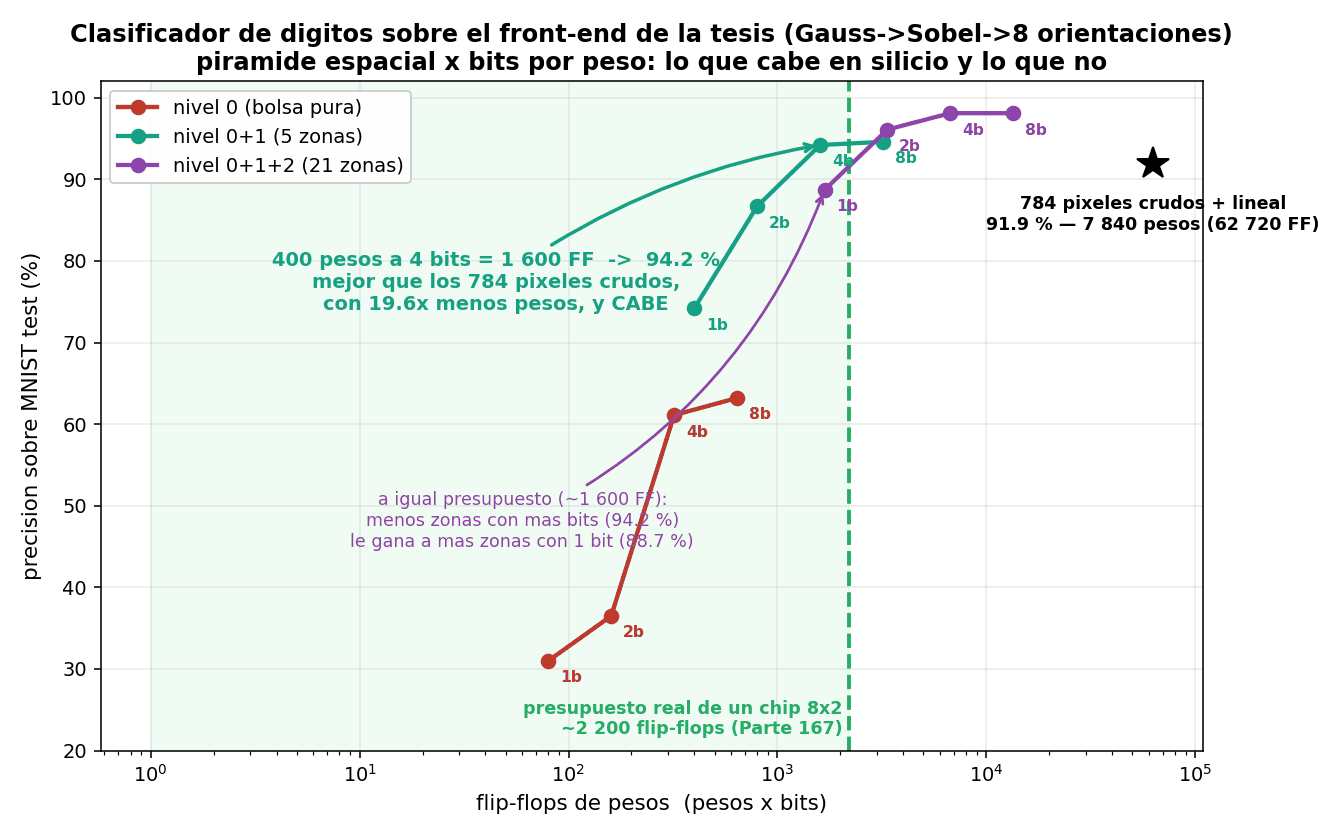
\includegraphics[keepaspectratio,alt={Figura 5.4. El espacio de diseño del clasificador, con el eje horizontal en escala logarítmica. Cada curva es un nivel de la pirámide espacial y cada punto una precisión de peso distinta. El hallazgo está en el cruce: 400 pesos de 4 bits ---1 600 biestables--- superan a los 784 píxeles crudos usando la vigésima parte de la memoria, y caben bajo el presupuesto real de un chip de 8×2 mosaicos, marcado con la línea vertical. A igualdad de memoria, la precisión de los pesos vale más que el número de zonas.}]{figuras/fig_5_4_espacio_de_diseno.png}}
\caption{\textbf{Figura 5.4.} El espacio de diseño del clasificador, con
el eje horizontal en escala logarítmica. Cada curva es un nivel de la
pirámide espacial y cada punto una precisión de peso distinta. El
hallazgo está en el cruce: \textbf{400 pesos de 4 bits ---1 600
biestables--- superan a los 784 píxeles crudos usando la vigésima parte
de la memoria}, y caben bajo el presupuesto real de un chip de 8×2
mosaicos, marcado con la línea vertical. A igualdad de memoria, la
precisión de los pesos vale más que el número de zonas.}
\end{figure}

\subsection{5.6.3 Lo que la exactitud no
muestra}\label{lo-que-la-exactitud-no-muestra}

Las medidas basadas en el \texttt{argmax} descartan la información de
los diez puntajes. Dos medidas que la conservan revelan una diferencia
que la exactitud oculta:

\begin{longtable}[]{@{}lrrr@{}}
\toprule\noalign{}
front-end & AUC macro & Brier & Brier skill \\
\midrule\noalign{}
\endhead
\bottomrule\noalign{}
\endlastfoot
SoC + Canny 1-salto & \textbf{0.9960} & \textbf{0.1465} &
\textbf{0.8371} \\
Canny 1-salto & 0.9957 & 0.1558 & 0.8268 \\
Sobel & 0.9945 & 0.1746 & 0.8059 \\
Canny transitivo & 0.9942 & \textbf{0.1991} & 0.7787 \\
SoC + Sobel & 0.9939 & 0.1749 & 0.8056 \\
\end{longtable}

El resultado de interés corresponde al Canny transitivo. En AUC ---que
mide el \textbf{ordenamiento}--- supera al SoC+Sobel; en Brier ---que
mide la \textbf{calibración}--- queda último por amplio margen.
\textbf{Ordena correctamente y decide mal.} Ello explica de forma
mecánica sus 139 falsos positivos: la reconstrucción morfológica
engruesa los contornos, el engrosamiento infla los histogramas, y el
criterio de rechazo ---que compara el mejor puntaje con el segundo---
deja hablar al circuito cuando debería callarlo.

\subsection{5.6.4 El punto de operación pesa más que el
front-end}\label{el-punto-de-operaciuxf3n-pesa-muxe1s-que-el-front-end}

Las comparaciones anteriores fijan el umbral y varían el filtro. El
experimento complementario ---fijar el filtro y \textbf{barrer el
umbral}--- arroja el resultado de mayor consecuencia práctica de esta
sección:

\begin{longtable}[]{@{}lrr@{}}
\toprule\noalign{}
magnitud & rango de exactitud & en unidades de σ \\
\midrule\noalign{}
\endhead
\bottomrule\noalign{}
\endlastfoot
el umbral, dentro del Sobel & \textbf{5.79 pp} & \textbf{4.4 σ} \\
el umbral, dentro del Canny & 0.90 pp & 0.7 σ \\
el filtro, cada uno en su óptimo & 0.38 pp & 0.3 σ \\
\end{longtable}

\textbf{Mover el umbral dentro del Sobel altera el resultado quince
veces más que cambiar de filtro.} Y la asimetría entre ambos front-ends
es el hallazgo: el Sobel presenta un óptimo estrecho ---su exactitud
recorre casi seis puntos a lo largo del rango útil--- mientras que el
Canny se mantiene en una meseta de nueve décimas. \textbf{El Canny en su
peor umbral supera al Sobel en diez de los once umbrales ensayados.}

El mecanismo reside en el algoritmo: el Sobel aplica un corte único y
nada recupera al píxel que queda por debajo; el Canny dispone de dos
umbrales y una histéresis que promueve el píxel débil adyacente a uno
fuerte. \textbf{La histéresis es un mecanismo de recuperación}, y de ahí
su insensibilidad.

\begin{quote}
\textbf{Consecuencia de diseño.} El front-end y el registro escribible
resuelven el mismo problema por vías distintas: el Canny adquiere
\textbf{en hardware} ---un \emph{line-buffer} adicional y ocho
comparaciones--- buena parte de la robustez que el Sobel obtiene
mediante \textbf{un procesador} capaz de reescribir el umbral. No son
decisiones que se sumen: son, en buena medida, \textbf{alternativas}.
\end{quote}

\subsection{5.6.5 El RTL contra el modelo, sobre el conjunto
completo}\label{el-rtl-contra-el-modelo-sobre-el-conjunto-completo}

Las cifras anteriores son del modelo en Python. La pregunta que decide
si sirven de algo es si el circuito las reproduce, y se respondió por el
camino más exigente disponible: \textbf{ejecutar el RTL sobre las diez
mil imágenes de prueba} en el simulador y comparar, no los porcentajes
agregados, sino cada predicción con la del modelo.

\begin{longtable}[]{@{}
  >{\raggedright\arraybackslash}p{(\linewidth - 2\tabcolsep) * \real{0.5000}}
  >{\raggedright\arraybackslash}p{(\linewidth - 2\tabcolsep) * \real{0.5000}}@{}}
\toprule\noalign{}
\begin{minipage}[b]{\linewidth}\raggedright
Comparación
\end{minipage} & \begin{minipage}[b]{\linewidth}\raggedright
Resultado
\end{minipage} \\
\midrule\noalign{}
\endhead
\bottomrule\noalign{}
\endlastfoot
Predicciones idénticas & \textbf{10 000 / 10 000} \\
Exactitud del RTL / del modelo & \textbf{91.04 \% / 91.04 \%} \\
Matriz de confusión & idéntica elemento por elemento \\
Veredictos de la clase de rechazo & \textbf{10 000 / 10 000}
idénticos \\
Cuadros aceptados · precisión al responder & 8 838 (88.38 \%) · 95.44
\%, en ambos \\
\end{longtable}

\begin{figure}
\centering
\pandocbounded{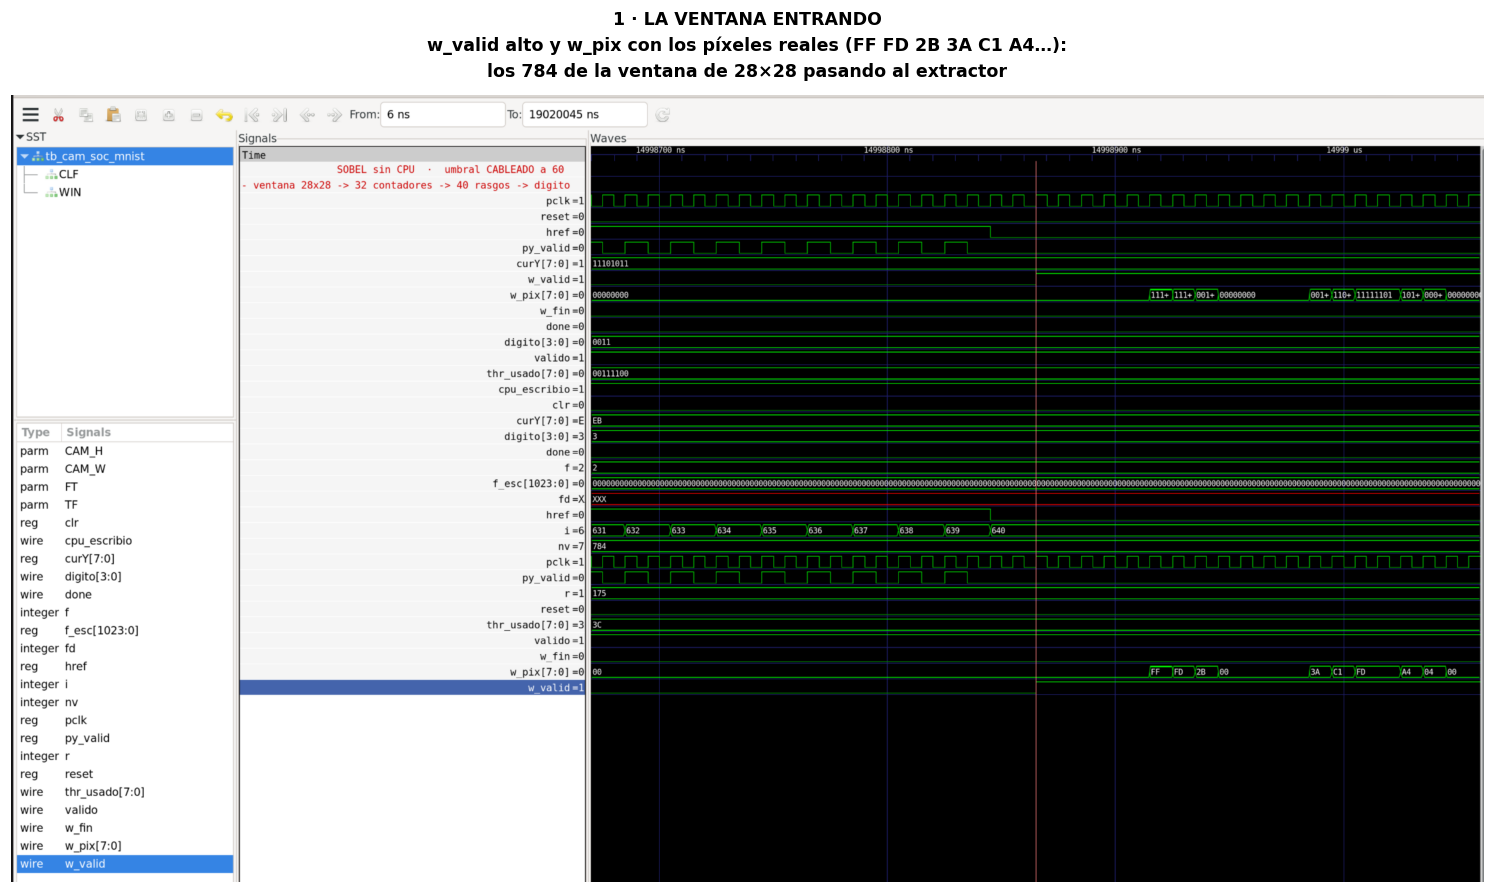
\includegraphics[keepaspectratio,alt={Figura 5.5. La ventana de 28×28 entrando al extractor, vista en el simulador. La señal w\_valid marca cada píxel válido y w\_pix lleva su valor ---FF FD 2B 3A C1 A4\ldots---; los 784 de la ventana pasan uno a uno antes de que done presente un dígito. Es el nivel al que se hizo la comparación contra el modelo: no se compararon porcentajes, se compararon señales.}]{figuras/fig_5_5_ventana_al_extractor.png}}
\caption{\textbf{Figura 5.5.} La ventana de 28×28 entrando al extractor,
vista en el simulador. La señal \texttt{w\_valid} marca cada píxel
válido y \texttt{w\_pix} lleva su valor
---\texttt{FF\ FD\ 2B\ 3A\ C1\ A4}\ldots---; los 784 de la ventana pasan
uno a uno antes de que \texttt{done} presente un dígito. Es el nivel al
que se hizo la comparación contra el modelo: no se compararon
porcentajes, se compararon señales.}
\end{figure}

No son cifras «parecidas» ni «dentro del margen de error»: \textbf{las
diez mil predicciones y los diez mil veredictos coinciden uno por uno},
y la matriz de confusión es la misma casilla por casilla. La
verificación de los filtros de la §5.1 se hizo sobre cinco imágenes;
ésta se hizo sobre diez mil, e incluye la decisión de rechazo, que es
lógica de comparación y no de aritmética.

\begin{quote}
Conviene precisar el alcance, porque más adelante aparece una cifra
distinta. Lo que aquí es exacto es el \textbf{clasificador completo}
---descriptor, pesos y decisión--- evaluado imagen por imagen. El 99.91
\% que informa la §5.6.6 se refiere a otra comparación: la del
\textbf{extractor de bordes} píxel a píxel dentro de la cadena, cuyas
discrepancias se concentran en la última fila del cuadro y no alteran
ninguna de las diez mil clasificaciones. Son dos medidas de objetos
distintos y no se contradicen.
\end{quote}

\subsection{5.6.6 Validación física}\label{validaciuxf3n-fuxedsica}

La validación sobre la placa se realizó en dos ensayos distintos, que
miden cosas distintas y cuyos resultados no deben confundirse.

\begin{figure}
\centering
\pandocbounded{
\includegraphics[keepaspectratio,alt={Figura 5.6. La cadena completa ---cámara, procesador, filtro y clasificador--- en señales, sobre la escena del dígito 3. El panel A muestra los 19 ms de dos cuadros: el veredicto sale en el primero y no cambia en el segundo. El panel B captura el instante en que el procesador sustituye el umbral por omisión del RTL, 110, por el 90 que escribe el firmware, con el camino de datos todavía en reinicio. El panel C mide los 639,5 µs que tardan las 400 multiplicaciones-acumulaciones y el argmax.}]{figuras/fig_5_6_cadena_en_senales.png}}
\caption{\textbf{Figura 5.6.} La cadena completa ---cámara, procesador,
filtro y clasificador--- en señales, sobre la escena del dígito 3. El
panel A muestra los 19 ms de dos cuadros: el veredicto sale en el
primero y no cambia en el segundo. El panel B captura el instante en que
\textbf{el procesador sustituye el umbral por omisión del RTL, 110, por
el 90 que escribe el firmware}, con el camino de datos todavía en
reinicio. El panel C mide los 639,5 µs que tardan las 400
multiplicaciones-acumulaciones y el \texttt{argmax}.}
\end{figure}

\textbf{Primer ensayo: diez dígitos grabados en el propio bitstream.} Se
embebieron diez imágenes de MNIST en la memoria de configuración y se
hizo que el circuito informara sus veredictos por el puerto serie, sin
cámara. La placa acertó \textbf{ocho de los diez}, y lo relevante no son
los ocho aciertos sino los dos fallos: el circuito confunde el
\textbf{2} con un 0 y el \textbf{3} con un 8, \textbf{exactamente los
mismos dos dígitos y exactamente las mismas respuestas equivocadas} que
había dado la simulación del diseño completo. Ninguno de los diez cambió
de respuesta a lo largo de unas treinta repeticiones.

\begin{quote}
Reproducir un acierto puede ser casualidad; reproducir un error
específico y repetido, no. Este ensayo no mide la exactitud del sistema
---diez imágenes no son una medida estadística--- sino que
\textbf{cierra el último eslabón de la traducción}: el diseño
sintetizado, emplazado, ruteado y cargado en silicio se comporta como el
RTL verificado, errores incluidos.
\end{quote}

\begin{figure}
\centering
\pandocbounded{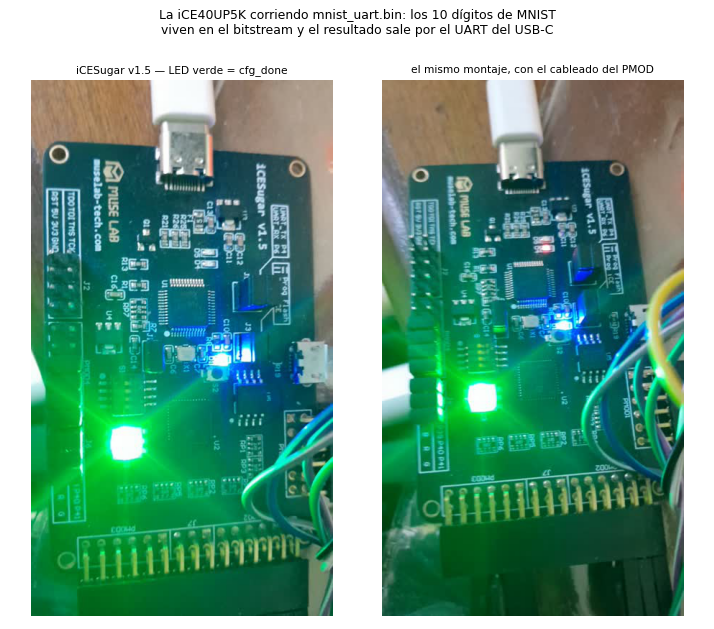
\includegraphics[keepaspectratio,alt={Figura 5.7. La tarjeta durante ese primer ensayo, con el mapa de bits cargado. El diodo verde está cableado a la señal de configuración terminada; el azul parpadea con el latido del sistema. Los diez veredictos salen por el puerto serie del mismo conector que alimenta la tarjeta. A la derecha, el mismo montaje con el cableado del módulo de pantalla ya conectado.}]{figuras/fig_5_7_la_placa_uart.png}}
\caption{\textbf{Figura 5.7.} La tarjeta durante ese primer ensayo, con
el mapa de bits cargado. El diodo verde está cableado a la señal de
configuración terminada; el azul parpadea con el latido del sistema. Los
diez veredictos salen por el puerto serie del mismo conector que
alimenta la tarjeta. A la derecha, el mismo montaje con el cableado del
módulo de pantalla ya conectado.}
\end{figure}

\textbf{Segundo ensayo: dígitos manuscritos ante la cámara.} El sistema
completo ---procesador RISC-V, periférico de umbrales, front-end Canny y
clasificador--- se enfrentó a dígitos escritos a mano y captados por una
cámara OV7670. \textbf{El circuito reconoció nueve de diez dígitos},
coincidiendo exactamente con lo que la simulación había predicho para
esa configuración.

Ese acuerdo, sin embargo, no se obtuvo al primer intento, y la causa
merece registrarse porque es la única discrepancia entre simulación y
silicio de todo el trabajo. En la primera versión la placa respondía
\textbf{ocho de diez} mientras la simulación sostenía nueve. El umbral
inferior del front-end se leía desde el módulo de control mediante una
\textbf{referencia jerárquica} ---\texttt{SOC.flt\_tlo}--- en lugar de
un puerto declarado. Ambas herramientas aceptaron el archivo sin una
sola advertencia y construyeron circuitos distintos: \texttt{iverilog}
resuelve la referencia y simula con el umbral escrito por el procesador,
mientras que el sintetizador crea un cable implícito de un bit que nadie
gobierna y fija el umbral inferior en cero. Sustituida la referencia por
un \textbf{puerto real}, la placa pasó a nueve de diez: el valor que la
simulación predecía.

\begin{quote}
\textbf{La lección no es que hubiera un error, sino dónde estaba.} El
RTL era legal, la simulación era correcta y la síntesis también lo era;
lo que falló fue suponer que ambas leían la misma descripción. Una
construcción que el lenguaje admite y que las dos herramientas
interpretan de forma distinta es indetectable por inspección y
silenciosa en los registros de ambas. Se deja escrita la regla de
trabajo que se adoptó a partir de aquí: \textbf{toda señal que cruce una
frontera de módulo se declara como puerto}, aunque el simulador acepte
el atajo.
\end{quote}

La verificación del extractor contra su modelo de referencia arrojó
\textbf{99.91 \%} de coincidencia exacta píxel a píxel para el Sobel y
\textbf{99.93 \%} para el Canny, concentrándose las diferencias en la
última fila del cuadro.

\subsection{5.6.7 Implementación en
silicio}\label{implementaciuxf3n-en-silicio}

El reconocedor se llevó a tecnología \texttt{sky130\_fd\_sc\_hd} en dos
variantes, ejecutando el flujo completo de OpenLane hasta la firma del
GDS:

\begin{longtable}[]{@{}lrr@{}}
\toprule\noalign{}
magnitud & Sobel & Canny 1-salto \\
\midrule\noalign{}
\endhead
\bottomrule\noalign{}
\endlastfoot
área del \emph{die} & 0.845 mm² & 0.890 mm² \\
celdas tras síntesis & 16 718 & 17 373 \\
celdas emplazadas & 19 949 & 20 921 \\
período de reloj & 30 ns (33.3 MHz) & 30 ns (33.3 MHz) \\
holgura con parásitos (\texttt{spef\_wns}) & \textbf{0.00 ns} &
\textbf{0.00 ns} \\
DRC · LVS · XOR & 0 · 0 · 0 & 0 · 0 · 0 \\
\end{longtable}

Ambos circuitos cierran el temporizado con los parásitos del
interconexionado extraídos y superan las tres verificaciones de firma
sin observaciones. Merece señalarse que \textbf{cierran más rápido que
los circuitos de visión equivalentes} ---que requirieron 32 y 36 ns---,
lo que resulta coherente con la ausencia de memoria de cuadro: es el
multiplexor de lectura del \emph{framebuffer} el que constituye el
camino crítico de aquéllos.

\textbf{Son los primeros circuitos de este trabajo cuya salida no es una
imagen.} Los diez presentados en las secciones §5.3 y §5.4 procesan;
éstos reconocen.

\subsection{5.6.8 El costo relativo del front-end depende del
sistema}\label{el-costo-relativo-del-front-end-depende-del-sistema}

La comparación de área entre ambos front-ends admite cuatro niveles de
integración. Las cuatro filas están en \textbf{celdas emplazadas}, la
misma escala de la §5.3, de modo que los cocientes son directamente
comparables entre sí:

\begin{longtable}[]{@{}
  >{\raggedright\arraybackslash}p{(\linewidth - 6\tabcolsep) * \real{0.2000}}
  >{\raggedleft\arraybackslash}p{(\linewidth - 6\tabcolsep) * \real{0.2667}}
  >{\raggedleft\arraybackslash}p{(\linewidth - 6\tabcolsep) * \real{0.2667}}
  >{\raggedleft\arraybackslash}p{(\linewidth - 6\tabcolsep) * \real{0.2667}}@{}}
\toprule\noalign{}
\begin{minipage}[b]{\linewidth}\raggedright
nivel
\end{minipage} & \begin{minipage}[b]{\linewidth}\raggedleft
Sobel
\end{minipage} & \begin{minipage}[b]{\linewidth}\raggedleft
Canny
\end{minipage} & \begin{minipage}[b]{\linewidth}\raggedleft
factor
\end{minipage} \\
\midrule\noalign{}
\endhead
\bottomrule\noalign{}
\endlastfoot
filtro aislado & 5 823 & 12 993 & \textbf{2.23×} \\
con procesador & 12 043 & 22 054 & 1.83× \\
sistema de visión completo & 35 653 & 41 925 & 1.18× \\
reconocedor con procesador & 19 949 & 20 921 & 1.05× \\
\textbf{reconocedor que además muestra} & \textbf{38 643} & \textbf{39
794} & \textbf{1.03×} \\
\end{longtable}

\textbf{El sobrecosto del Canny se diluye conforme crece el sistema que
lo rodea.} Considerado de forma aislada cuesta un \textbf{123 \%} más;
con un procesador al lado, un 83 \%; dentro de un sistema de visión, un
18 \%; integrado en un reconocedor, un 5 \%; y en un reconocedor que
además dibuja en pantalla, un \textbf{3 \%}. El motivo es que el
clasificador ---histograma, pirámide y 400 multiplicaciones--- es
idéntico en ambas variantes y domina el área, mientras que la diferencia
se reduce al tercer \emph{line-buffer}.

De ello se sigue una conclusión condicional: \textbf{el Sobel aventaja
al Canny en área únicamente cuando el filtro constituye el circuito
completo.} En un sistema que reconoce, esa ventaja ---la única que el
Sobel conserva, según §5.6.2 a §5.6.4--- deja de ser determinante.

\begin{center}\rule{0.5\linewidth}{0.5pt}\end{center}

\subsection{Referencias de la
sección}\label{referencias-de-la-secciuxf3n}

\begin{itemize}
\tightlist
\item
  Chow, C. K. (1970). \emph{On Optimum Recognition Error and Reject
  Tradeoff.} IEEE Trans. Inf. Theory, 16(1), 41-46.
\item
  Dalal, N. y Triggs, B. (2005). \emph{Histograms of Oriented Gradients
  for Human Detection.} CVPR, 886-893.
\item
  Lazebnik, S., Schmid, C. y Ponce, J. (2006). \emph{Beyond Bags of
  Features: Spatial Pyramid Matching.} CVPR, 2169-2178.
\item
  Lowe, D. G. (2004). \emph{Distinctive Image Features from
  Scale-Invariant Keypoints.} IJCV, 60(2), 91-110.
\end{itemize}

\section{5.7 Verificación eléctrica del camino
crítico}\label{verificaciuxf3n-eluxe9ctrica-del-camino-cruxedtico}

\begin{quote}
\textbf{Estado:} borrador 1, 2026-09-21. Fuente: cuaderno 2, §33. Todas
las cifras de esta sección proceden de corridas de NGSpice sobre
\texttt{sky130\_fd\_sc\_hd} en la esquina típica, 1,8 V y 25 °C, y de
los ficheros de parásitos extraídos de los dos reconocedores.
\end{quote}

Las secciones anteriores aceptaron sin discusión lo que el analizador de
tiempos informa. Ésta pregunta si ese número es correcto, y lo hace por
el único camino que no depende de la misma herramienta: \textbf{resolver
los transistores}.

La pregunta no es ociosa. Un analizador estático no simula: consulta
tablas caracterizadas de antemano e interpola. Es rapidísimo y es lo que
permite firmar un circuito de doscientas mil instancias, pero entre su
respuesta y la física median un modelo de celda, un modelo de cable y un
procedimiento de interpolación. Comprobar cuánto de lo que informa
sobrevive a una simulación eléctrica es, por tanto, una verificación del
instrumento y no del circuito.

\subsection{5.7.1 Por qué el camino crítico y no el
chip}\label{por-quuxe9-el-camino-cruxedtico-y-no-el-chip}

Simular los dos reconocedores enteros no es inviable por tamaño
---\texttt{pan\_sobel} tiene 116 314 transistores y en este trabajo ya
se simuló un procesador de 121 310--- sino \textbf{por tiempo}: para que
el clasificador vea sus 784 píxeles hay que hacerle entrar un cuadro
completo, y eso son 633 800 ciclos, unos treinta y dos veces más
actividad que la simulación de procesador ya realizada.

El camino crítico, en cambio, son \textbf{treinta y siete celdas} en un
chip y treinta y seis en el otro. Se extrajeron del reporte del
analizador, se reconstruyeron como cadena aislada con la carga y la
pendiente que el propio reporte declara en cada etapa, y se resolvieron
en NGSpice.

\subsection{5.7.2 El resultado}\label{el-resultado}

Se aplicaron cinco variantes del mismo banco, cada una añadiendo un
ingrediente al anterior, de modo que la diferencia entre dos renglones
consecutivos aísla la contribución de ese ingrediente:

\begin{longtable}[]{@{}
  >{\raggedright\arraybackslash}p{(\linewidth - 4\tabcolsep) * \real{0.2727}}
  >{\raggedleft\arraybackslash}p{(\linewidth - 4\tabcolsep) * \real{0.3636}}
  >{\raggedleft\arraybackslash}p{(\linewidth - 4\tabcolsep) * \real{0.3636}}@{}}
\toprule\noalign{}
\begin{minipage}[b]{\linewidth}\raggedright
\end{minipage} & \begin{minipage}[b]{\linewidth}\raggedleft
\texttt{pan\_sobel} (37 etapas)
\end{minipage} & \begin{minipage}[b]{\linewidth}\raggedleft
\texttt{pan\_canny} (36 etapas)
\end{minipage} \\
\midrule\noalign{}
\endhead
\bottomrule\noalign{}
\endlastfoot
\textbf{Analizador estático, con parásitos} & \textbf{12,230 ns} &
\textbf{9,890 ns} \\
A · las puertas solas & 4,646 ns & 4,424 ns \\
B · más la capacitancia extraída, agrupada & 8,159 ns & 7,552 ns \\
C · más la pendiente de entrada real & 8,178 ns & 7,588 ns \\
D0 · más la topología del fichero de parásitos, \textbf{con R = 0} &
7,603 ns & 7,022 ns \\
D · más la \textbf{resistencia medida} de cada tramo & 7,620 ns & 7,043
ns \\
E · más la \textbf{celda extraída del \emph{layout}} & \textbf{9,694 ns}
& \textbf{8,962 ns} \\
\emph{fracción del retardo que la simulación reproduce} & \emph{79,3 \%}
& \emph{90,6 \%} \\
\end{longtable}

La variante \textbf{D0 es un control}, idéntica a la D salvo en que sus
resistencias valen cero. Sin ella, el efecto de la resistencia y el de
\emph{repartir} la capacitancia a lo largo del árbol en vez de agruparla
en un nodo quedarían sumados en una sola cifra y no podrían separarse.

\begin{figure}
\centering
\pandocbounded{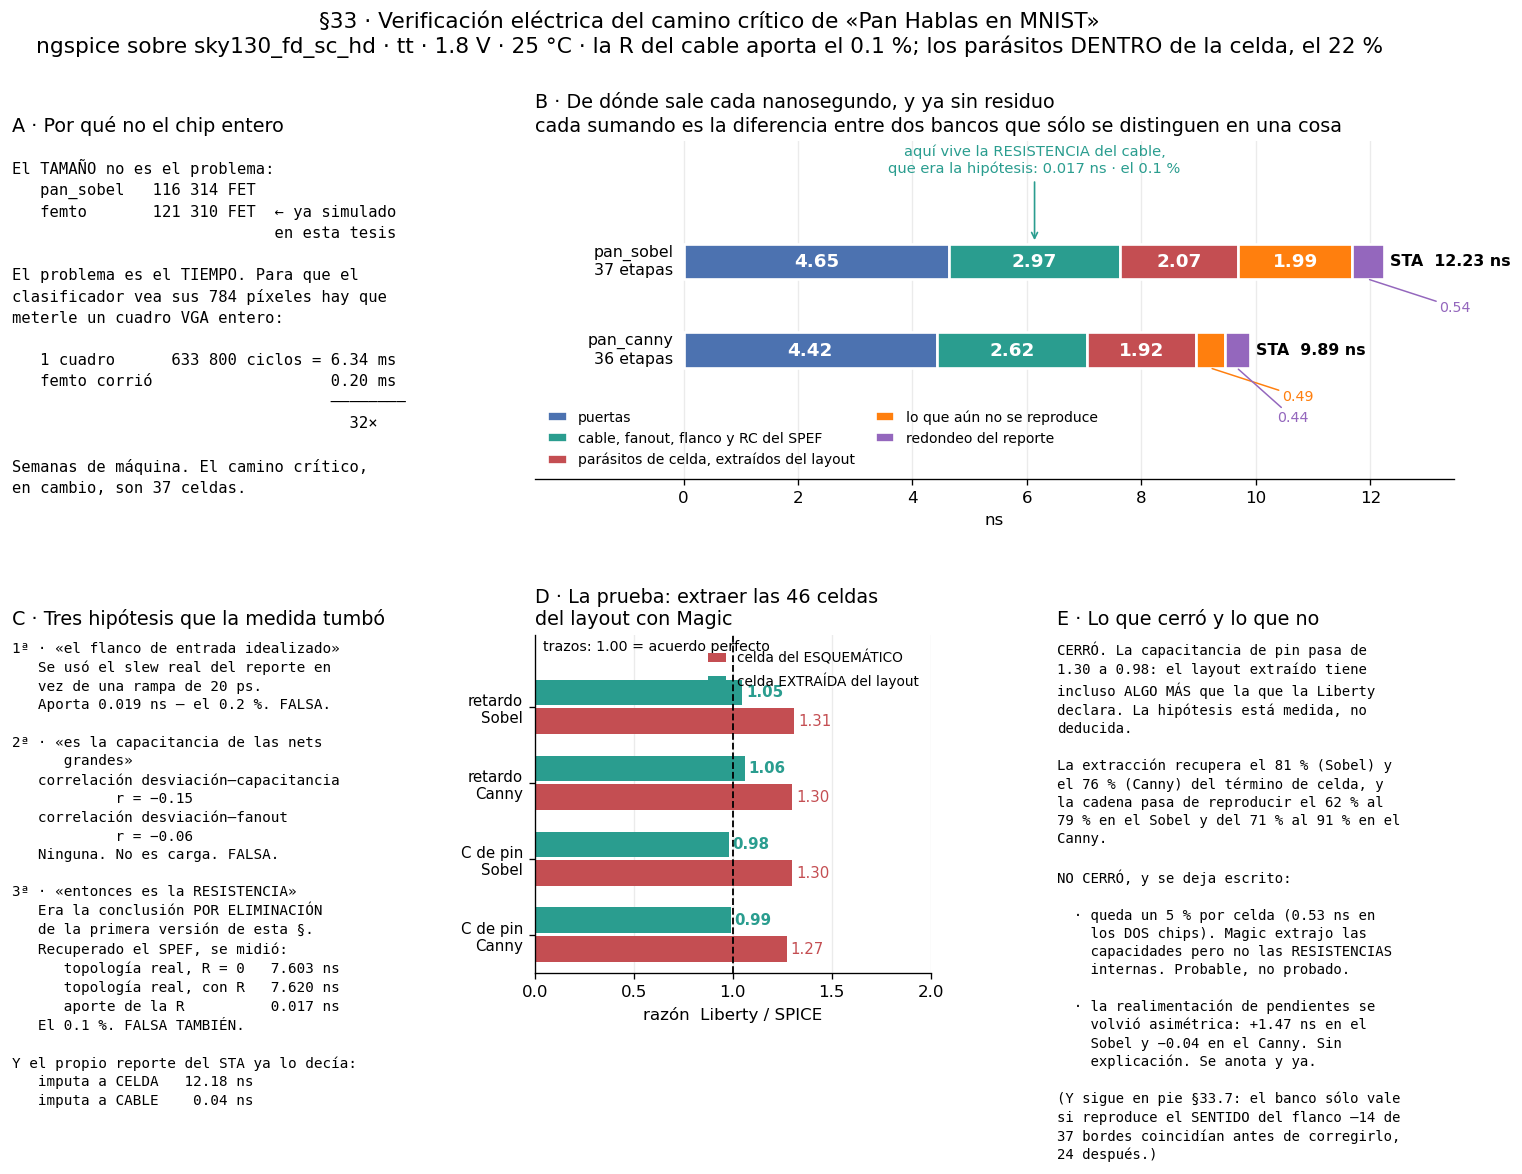
\includegraphics[keepaspectratio,alt={Figura 5.8. El desglose completo de la verificación. El panel A explica por qué se simula el camino y no el chip; el B reparte los 12,23 ns del pan\_sobel y los 9,89 del pan\_canny en sumandos que no dejan residuo; el C recoge las tres hipótesis que la medida desmintió; el D contrapone la celda del esquemático con la extraída del dibujo en los dos experimentos independientes; y el E separa lo que quedó cerrado de lo que se deja escrito como abierto.}]{figuras/fig_5_8_spice_desglose.png}}
\caption{\textbf{Figura 5.8.} El desglose completo de la verificación.
El panel A explica por qué se simula el camino y no el chip; el B
reparte los 12,23 ns del \texttt{pan\_sobel} y los 9,89 del
\texttt{pan\_canny} en sumandos que no dejan residuo; el C recoge las
tres hipótesis que la medida desmintió; el D contrapone la celda del
esquemático con la extraída del dibujo en los dos experimentos
independientes; y el E separa lo que quedó cerrado de lo que se deja
escrito como abierto.}
\end{figure}

\subsection{5.7.3 Tres explicaciones que la medida
desmintió}\label{tres-explicaciones-que-la-medida-desmintiuxf3}

Las tres parecían razonables, y conviene dejar constancia de las tres.

\textbf{El flanco de entrada idealizado.} El estímulo inicial era una
rampa de 20 ps, mucho más limpia que la transición que la primera etapa
recibe en el circuito; cabía esperar que un frente degradado se
propagase como retardo a lo largo de las treinta y siete etapas.
Sustituido por la pendiente real que el reporte declara, la contribución
resultó de \textbf{0,019 ns: el 0,2 \%}.

\textbf{La capacitancia de las redes grandes.} Las desviaciones mayores
se concentraban en puertas de muchas entradas, lo que sugería redes
largas y cargadas. Se midió la correlación entre la desviación de cada
etapa y su capacitancia: \textbf{r = −0,15}; y con el número de
destinos: \textbf{r = −0,06}. Ninguna de las dos sostiene la
explicación.

\textbf{La resistencia de la interconexión.} Descartadas las anteriores
quedaba ésta, y \textbf{así se dio por concluida la primera versión de
esta sección}: el analizador trabaja sobre el fichero de parásitos, que
informa resistencia y capacitancia de cada red, mientras que el reporte
de texto publica sólo la capacitancia, de modo que la simulación habría
recibido una descripción incompleta de los cables. La conjetura no pudo
comprobarse entonces porque ese fichero no se había conservado.

Recuperado, se midió. \textbf{La resistencia de la interconexión aporta
0,017 ns: el 0,1 \% del camino.} No los cuatro nanosegundos que había
que explicar.

\begin{quote}
\textbf{El propio reporte lo decía, y no se leyó.} El analizador imputa
cada retardo a un pin, y los de pin de salida son de celda mientras que
los de pin de entrada son de cable. Sumados por separado a lo largo del
camino: \textbf{12,18 ns imputados a celda y 0,04 ns a cable}. La
herramienta nunca atribuyó el tiempo a la interconexión. Bastaba con
sumar dos columnas.
\end{quote}

\subsection{5.7.4 La causa: la celda del esquemático no es la celda del
silicio}\label{la-causa-la-celda-del-esquemuxe1tico-no-es-la-celda-del-silicio}

Si la diferencia está dentro de las celdas, hay que preguntárselo a una
celda sola. El banco se redujo al mínimo ---una celda, el arco que el
camino recorre, la pendiente y la carga que el reporte declara--- y se
hizo la misma pregunta dos veces: a la tabla caracterizada, interpolando
como hace el analizador, y al simulador, resolviendo los transistores
que el kit de diseño distribuye.

La tabla reproduce al analizador casi exactamente, lo que confirma que
éste se limita a consultarla. La simulación, en cambio, queda
\textbf{sistemáticamente por debajo en treinta y cinco de las treinta y
siete etapas}, con una razón de \textbf{1,31} que no depende ni de la
carga ni de la pendiente. Esa independencia es la que descarta un
defecto del banco y señala a la celda misma.

La causa está en el fichero que se le entregó como modelo. El kit
distribuye el netlist \textbf{esquemático}: doce transistores y ni un
solo parásito. La biblioteca caracterizada, en cambio, se obtuvo sobre
la celda \textbf{dibujada}, con el metal, los contactos y la difusión
que el \emph{layout} añade. Al simulador se le describió la celda antes
de dibujarla.

Eso admite medición directa. Inyectando una rampa lenta en cada pin de
entrada e integrando la corriente ---capacitancia como carga dividida
por tensión, sin modelo ni supuesto--- la biblioteca atribuye a cada
pin, en promedio sobre los treinta y cinco del camino, \textbf{un 30 \%
más de capacitancia de la que el esquemático tiene}.

\begin{quote}
\textbf{Dos experimentos distintos, la misma cifra.} La razón entre el
retardo que la biblioteca declara y el que la simulación obtiene sobre
el esquemático es \textbf{1,31}. La razón entre la capacitancia que la
biblioteca declara y la que el esquemático tiene es \textbf{1,30}. Uno
mide tiempos y el otro mide carga, sobre las mismas treinta y siete
etapas.
\end{quote}

\textbf{La comprobación.} Lo anterior establece que al esquemático le
faltan parásitos, no que sean \emph{ésos} los que faltan. El kit no
distribuye el netlist de la celda dibujada, pero sí el dibujo: se
extrajeron con Magic las \textbf{cuarenta y seis celdas} que aparecen en
los dos caminos y se repitieron los dos experimentos sin cambiar nada
más.

\begin{longtable}[]{@{}
  >{\raggedright\arraybackslash}p{(\linewidth - 4\tabcolsep) * \real{0.2727}}
  >{\raggedleft\arraybackslash}p{(\linewidth - 4\tabcolsep) * \real{0.3636}}
  >{\raggedleft\arraybackslash}p{(\linewidth - 4\tabcolsep) * \real{0.3636}}@{}}
\toprule\noalign{}
\begin{minipage}[b]{\linewidth}\raggedright
razón biblioteca / simulación
\end{minipage} & \begin{minipage}[b]{\linewidth}\raggedleft
celda del \textbf{esquemático}
\end{minipage} & \begin{minipage}[b]{\linewidth}\raggedleft
celda \textbf{extraída}
\end{minipage} \\
\midrule\noalign{}
\endhead
\bottomrule\noalign{}
\endlastfoot
capacitancia de pin · \texttt{pan\_sobel} & 1,30 & \textbf{0,98} \\
capacitancia de pin · \texttt{pan\_canny} & 1,27 & \textbf{0,99} \\
retardo de celda aislada · \texttt{pan\_sobel} & 1,31 & \textbf{1,05} \\
retardo de celda aislada · \texttt{pan\_canny} & 1,30 & \textbf{1,06} \\
\end{longtable}

\textbf{La discrepancia de capacitancia desaparece.} La hipótesis queda
medida y no deducida, que era justamente lo que faltaba.

\subsection{5.7.5 La cuenta, y lo que queda
abierto}\label{la-cuenta-y-lo-que-queda-abierto}

Repartidos los 12,230 ns sin residuo, el término que importa sale igual
en los dos circuitos:

\begin{longtable}[]{@{}
  >{\raggedright\arraybackslash}p{(\linewidth - 4\tabcolsep) * \real{0.2727}}
  >{\raggedleft\arraybackslash}p{(\linewidth - 4\tabcolsep) * \real{0.3636}}
  >{\raggedleft\arraybackslash}p{(\linewidth - 4\tabcolsep) * \real{0.3636}}@{}}
\toprule\noalign{}
\begin{minipage}[b]{\linewidth}\raggedright
\end{minipage} & \begin{minipage}[b]{\linewidth}\raggedleft
\texttt{pan\_sobel}
\end{minipage} & \begin{minipage}[b]{\linewidth}\raggedleft
\texttt{pan\_canny}
\end{minipage} \\
\midrule\noalign{}
\endhead
\bottomrule\noalign{}
\endlastfoot
\textbf{el modelo de celda, como fracción del camino} & \textbf{22,6 \%}
& \textbf{22,1 \%} \\
resistencia de la interconexión & 0,1 \% & 0,2 \% \\
\end{longtable}

Dos circuitos distintos, dos caminos críticos que no comparten una sola
instancia, y la misma cifra a cuatro décimas de punto: \textbf{algo más
de la quinta parte del retardo de un camino crítico la ponen los
parásitos que el dibujo añade dentro de las celdas.}

\begin{figure}
\centering
\pandocbounded{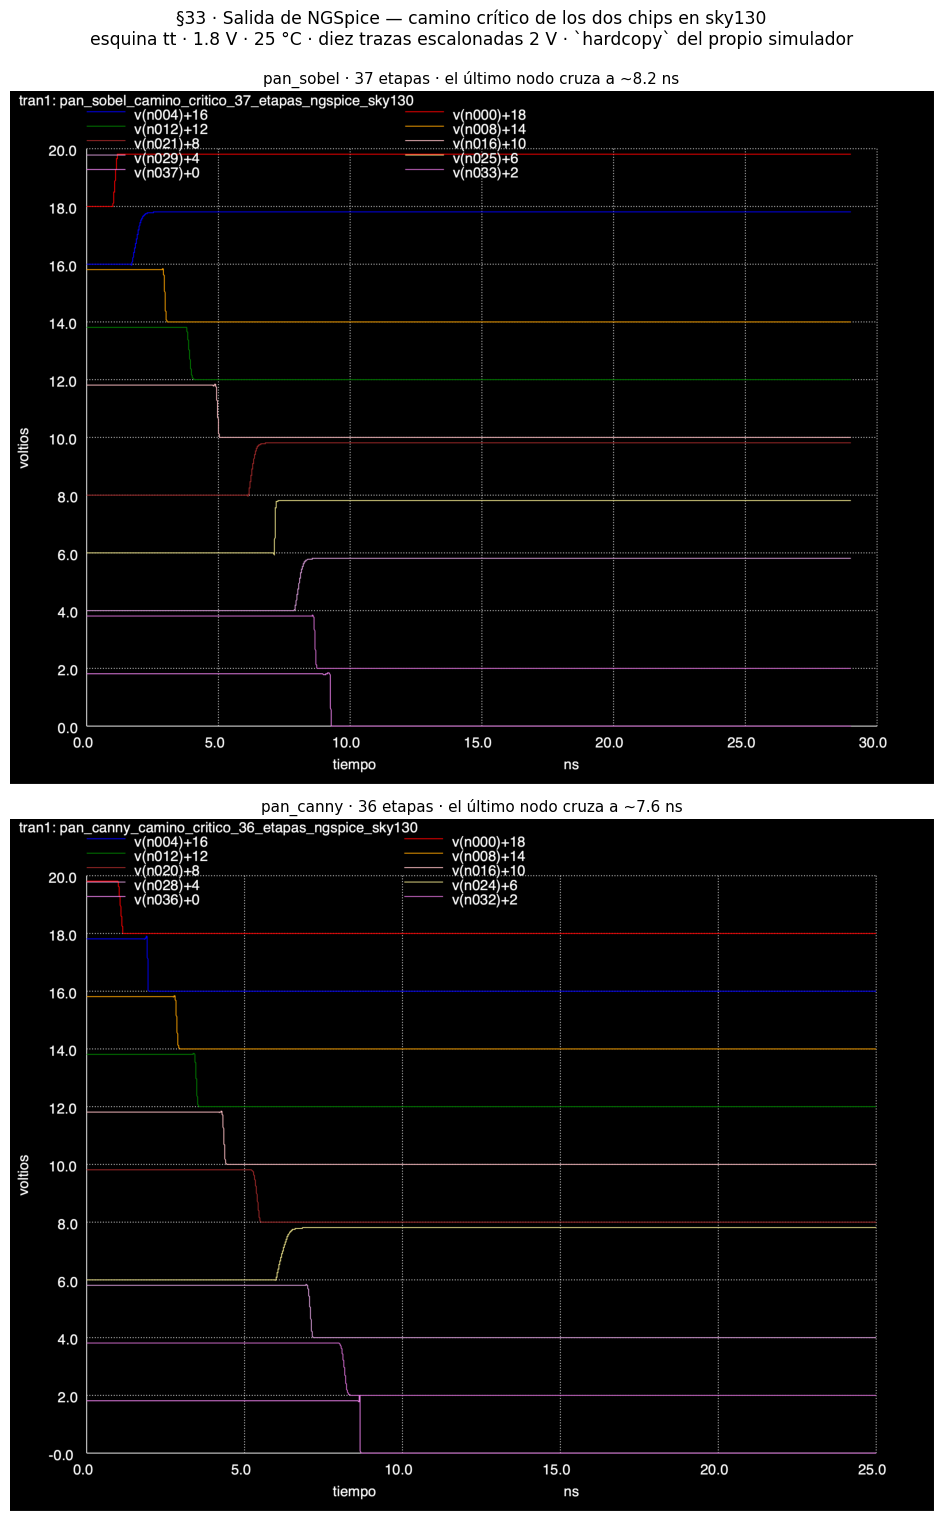
\includegraphics[keepaspectratio,alt={Figura 5.9. La salida del simulador, tal como éste la dibuja. Cada traza es un nodo del camino crítico, desplazada dos voltios respecto de la anterior para que las diez quepan en el mismo eje; la cascada de transiciones de arriba abajo es la señal propagándose etapa por etapa. El último nodo del pan\_sobel conmuta a unos 8,2 ns y el del pan\_canny a unos 7,6, que son las variantes D de la tabla anterior.}]{figuras/fig_5_9_spice_ondas.png}}
\caption{\textbf{Figura 5.9.} La salida del simulador, tal como éste la
dibuja. Cada traza es un nodo del camino crítico, desplazada dos voltios
respecto de la anterior para que las diez quepan en el mismo eje; la
cascada de transiciones de arriba abajo es la señal propagándose etapa
por etapa. El último nodo del \texttt{pan\_sobel} conmuta a unos 8,2 ns
y el del \texttt{pan\_canny} a unos 7,6, que son las variantes D de la
tabla anterior.}
\end{figure}

\textbf{Lo que no cerró, y se deja escrito.} Queda un 5 \% por celda
---0,528 ns en un chip y 0,530 en el otro, prácticamente el mismo valor
absoluto en dos caminos distintos--- que la extracción no recupera. La
explicación más probable es que el procedimiento empleado conserva las
\textbf{capacidades} internas de la celda pero no sus
\textbf{resistencias}, de modo que su metal interno sigue comportándose
como un cortocircuito ideal. Se anota como \textbf{probable y no
comprobada}. Y la realimentación de pendientes a lo largo de la cadena
resulta asimétrica entre los dos chips ---+1,47 ns en uno y −0,04 en el
otro--- sin explicación disponible.

\begin{quote}
\textbf{La conclusión.} El simulador y el analizador no discrepan sobre
la física: discrepan sobre el circuito. Al analizador se le describió la
celda tal como quedó en el \emph{layout}; al simulador, tal como estaba
en el esquema.

La verificación eléctrica no midió, por tanto, que el analizador se
equivocara. Midió \textbf{cuánto del retardo de un circuito integrado lo
pone el dibujo y no el esquema}: algo más de la quinta parte, y la misma
fracción en dos chips independientes. Es una cifra más útil que la que
se buscaba, y explica por qué ninguna implementación puede firmarse
sobre el esquemático.
\end{quote}

\chapter{6. Discusión}\label{discusiuxf3n}

\begin{quote}
\textbf{Estado:} borrador 1, escrito el 2026-09-21. Fuente: cuadernos 1
y 2, y el Capítulo 5. Formato Markdown para convertir con
\texttt{pandoc}.
\end{quote}

El capítulo anterior presentó mediciones. Éste sostiene afirmaciones. La
diferencia importa: una medición es un hecho que se comprueba repitiendo
el experimento, mientras que una afirmación es una lectura de varios
hechos y puede ser equivocada aunque todos ellos sean correctos. Este
trabajo tuvo que retractar dos afirmaciones de ese tipo durante su
desarrollo, y la experiencia dejó una disciplina que se aplica aquí:
\textbf{cada tesis de este capítulo señala qué medición la sostiene y
qué otra lectura descarta.}

\section{6.1 Lo que decide si un algoritmo cabe no es el
algoritmo}\label{lo-que-decide-si-un-algoritmo-cabe-no-es-el-algoritmo}

Ésta es la afirmación central del trabajo, y la más contraintuitiva para
quien llega desde el software.

Los tres filtros implementados ejecutan aritmética comparable. Ninguno
multiplica; los tres recorren la imagen aplicando una ventana de 3×3 y
comparando contra un umbral. Si el costo en silicio siguiera a la
complejidad aritmética, los tres deberían costar aproximadamente lo
mismo. La §5.4.3 midió lo contrario:

\begin{longtable}[]{@{}llr@{}}
\toprule\noalign{}
desde & hasta & cuesta \\
\midrule\noalign{}
\endhead
\bottomrule\noalign{}
\endlastfoot
Sobel & Canny de un salto & \textbf{+5 851 celdas} \\
Canny de un salto & Canny transitivo & \textbf{+94 511 celdas} \\
\end{longtable}

Ampliar el alcance de la ventana en un salto cuesta menos de seis mil
celdas. Ampliarlo al cuadro completo cuesta \textbf{noventa y cuatro mil
quinientas once}. Y la causa no está en las operaciones sino en
\textbf{cuánto estado hay que sostener a la vez}: los dos primeros
filtros procesan en flujo y retienen unas pocas líneas; el tercero
necesita el cuadro entero residente y accesible en orden arbitrario,
porque su punto fijo puede propagar una decisión desde cualquier píxel
hacia cualquier otro.

La comparación que resume el capítulo es ésta: \textbf{un procesador
RISC-V completo, con su memoria de programa y su periférico, cuesta
alrededor de nueve mil celdas} ---medido tres veces, sobre los tres
filtros, con una dispersión inferior al 5 \%--- \textbf{es decir,
aproximadamente la décima parte de lo que cuesta cambiar el alcance del
patrón de local a global.}

\begin{quote}
Dicho de otro modo: en el presupuesto de este chip, \textbf{meter un
procesador entero es una decisión menor comparada con decidir cuánta
imagen mira el filtro}. Es exactamente lo contrario de lo que sugiere la
intuición formada en software, donde el procesador es el recurso caro y
la memoria se pide al sistema operativo.
\end{quote}

\subsection{Las tres caras del mismo
precio}\label{las-tres-caras-del-mismo-precio}

El costo de la memoria no se cobra sólo en área. La §5.4.1 muestra que
\textbf{los dos circuitos transitivos son también los dos únicos que no
cierran temporizado}, con −19,35 ns y −18,23 ns de holgura una vez
extraídos los parásitos. El multiplexor que lee un framebuffer de miles
de entradas es un camino largo por construcción, y a partir de cierto
tamaño deja de ser caro para volverse inviable.

Y se cobra en manufacturabilidad. La §5.3 documenta que los diseños con
framebuffer grande acumulan un número de violaciones de antena muy
superior al resto, porque las redes de direccionamiento son largas y
ramificadas.

\textbf{Área, frecuencia y manufacturabilidad son tres manifestaciones
del mismo hecho}, y conviene presentarlas juntas: un diseñador que
optimice sólo el área concluirá que el framebuffer es aceptable, porque
sólo verá un tercio del problema.

\section{6.2 El costo se movió; no se
eliminó}\label{el-costo-se-moviuxf3-no-se-eliminuxf3}

Una lectura apresurada del clasificador de la §5.6 sugeriría que la
solución al problema anterior es sustituir memoria por lógica. El
trabajo permite matizar eso con números propios.

El clasificador de dígitos alcanza 91,04 \% sobre MNIST con \textbf{400
pesos de cuatro bits} ---doscientos bytes--- frente al 91,9 \% que
obtienen los 784 píxeles crudos con 7 840 pesos. La memoria se redujo en
un factor de veinte y la exactitud no se movió. Es un resultado fuerte,
y se enuncia así en la §5.6.

Pero el descriptor que hace posible esa reducción ---histograma de
orientaciones por zona, sobre bordes--- \textbf{no es gratuito}: hay que
calcularlo, y calcularlo es lógica. Las etapas cableadas que lo producen
cuestan decenas de miles de celdas.

\begin{quote}
La conclusión honesta no es «la codificación inteligente elimina el
costo» sino \textbf{«la codificación inteligente mueve el costo de
memoria a lógica»}, y eso es valioso únicamente porque en este sustrato
la memoria es el recurso caro. En una FPGA con bloques de memoria
disponibles, la misma decisión sería indiferente o incluso perjudicial.
\end{quote}

\section{6.3 Quién fija el reloj cambia con lo que se mete en el
chip}\label{quiuxe9n-fija-el-reloj-cambia-con-lo-que-se-mete-en-el-chip}

Los resultados del Capítulo 5 permiten seguir el camino crítico a lo
largo de una familia de diseños y observar que \textbf{el responsable
cambia tres veces}:

\begin{longtable}[]{@{}
  >{\raggedright\arraybackslash}p{(\linewidth - 2\tabcolsep) * \real{0.5000}}
  >{\raggedright\arraybackslash}p{(\linewidth - 2\tabcolsep) * \real{0.5000}}@{}}
\toprule\noalign{}
\begin{minipage}[b]{\linewidth}\raggedright
Diseño
\end{minipage} & \begin{minipage}[b]{\linewidth}\raggedright
Quién fija la frecuencia
\end{minipage} \\
\midrule\noalign{}
\endhead
\bottomrule\noalign{}
\endlastfoot
Filtros solos & el camino de datos del filtro \\
Con procesador & \textbf{el FemtoRV32} \\
Con framebuffer grande & \textbf{el multiplexor de lectura del
framebuffer} \\
\end{longtable}

Es un resultado útil para quien planifique un sistema parecido, porque
implica que \textbf{optimizar el bloque que fue crítico en el diseño
anterior puede no mejorar nada}. La pregunta «¿qué limita mi
frecuencia?» no tiene una respuesta estable: tiene una respuesta por
configuración.

\section{6.4 Integrar no es sumar, pero sólo cuando el temporizado
aprieta}\label{integrar-no-es-sumar-pero-suxf3lo-cuando-el-temporizado-aprieta}

Dos observaciones de este trabajo parecen contradecirse, y el matiz está
en la diferencia.

Al integrar el procesador con el filtro Canny en un die apretado, el
resultado superó la predicción ingenua ---la suma de las partes--- en
unas 6 500 celdas. En otro diseño de la misma familia, con die holgado y
reloj relajado, el resultado quedó un \textbf{1,6 \% por debajo} de esa
predicción.

Las dos medidas son correctas. Lo que las separa es \textbf{si el flujo
tuvo que trabajar para cerrar temporizado}: cuando lo tuvo, insertó
amortiguadores y redimensionó celdas, y ese trabajo se cobra en área;
cuando no, el optimizador pudo además compartir lógica entre bloques y
el total salió menor que la suma.

\begin{quote}
La regla que se deja escrita no es «integrar cuesta más» sino:
\textbf{la penalización de integración no es una propiedad del diseño
sino del margen con que se le pide cerrar.} Un mismo sistema puede
costar más o menos que sus partes según el reloj que se le exija.
\end{quote}

\section{6.5 La restricción mueve la frontera entre software y
hardware}\label{la-restricciuxf3n-mueve-la-frontera-entre-software-y-hardware}

El episodio de la §5.2.4 es el ejemplo más claro de co-diseño de este
trabajo, y conviene leerlo con cuidado porque su lección no es la
evidente.

La histéresis transitiva calculada por software funcionaba correctamente
en simulación. Al intentar sintetizar el conjunto sobre la iCE40UP5K la
ocupación llegó al \textbf{127 \%}. Trasladada a hardware como camino de
datos, la misma función ocupa el \textbf{33 \%}.

Lo interesante no es que el hardware sea más eficiente, que es
esperable. Es que \textbf{la frontera entre lo que ejecuta el procesador
y lo que ejecuta la lógica dedicada no la fijó una preferencia de diseño
sino una medición de recursos}. Y que esa frontera \textbf{se mueve con
el sustrato}: en el ASIC, donde el área no está acotada por un
dispositivo fijo, el procesador vuelve a ser viable junto al transitivo
y cuesta las mismas nueve mil celdas que junto a cualquier otro filtro.

La misma pregunta de diseño tiene respuestas opuestas en los dos
destinos, y ninguna de las dos es incorrecta.

\section{6.6 El front-end y el procesador son alternativas, no
complementos}\label{el-front-end-y-el-procesador-son-alternativas-no-complementos}

Éste es el aporte de ingeniería que el trabajo propone, y se apoya en
tres mediciones independientes.

\textbf{Primera.} Los dos filtros no se distinguen en exactitud de
clasificación: 0,38 pp entre ellos (§5.6). El Canny no reconoce mejor.

\textbf{Segunda.} Sí se distinguen en \textbf{sensibilidad al punto de
operación}. Mover el umbral cambia el resultado del Sobel en
\textbf{5,79 pp} y el del Canny en \textbf{0,90 pp}. El Sobel vive en un
pico angosto del espacio de parámetros; el Canny, en una meseta.

\textbf{Tercera.} Un Sobel sensible al umbral necesita que alguien se lo
ajuste en tiempo de ejecución, y para eso está el procesador con su
periférico. Un Canny insensible no lo necesita.

Poniendo precio a las dos soluciones sobre el mismo silicio:

\begin{longtable}[]{@{}
  >{\raggedright\arraybackslash}p{(\linewidth - 4\tabcolsep) * \real{0.3000}}
  >{\raggedright\arraybackslash}p{(\linewidth - 4\tabcolsep) * \real{0.3000}}
  >{\raggedleft\arraybackslash}p{(\linewidth - 4\tabcolsep) * \real{0.4000}}@{}}
\toprule\noalign{}
\begin{minipage}[b]{\linewidth}\raggedright
lo que se compra
\end{minipage} & \begin{minipage}[b]{\linewidth}\raggedright
dónde
\end{minipage} & \begin{minipage}[b]{\linewidth}\raggedleft
cuesta
\end{minipage} \\
\midrule\noalign{}
\endhead
\bottomrule\noalign{}
\endlastfoot
robustez al umbral \textbf{en el front-end} & el Canny, en el
reconocedor & \textbf{972 celdas} \\
robustez al umbral \textbf{por software} & el procesador y su periferia
& \textbf{6 220 celdas} \\
\end{longtable}

\begin{figure}
\centering
\pandocbounded{
\includegraphics[keepaspectratio,alt={Figura 6.1. El balance completo entre los dos filtros, sobre seis parejas de circuitos con plano firmado. El panel A los compara en celdas; el B muestra el sobrecoste del Canny cayendo del 123 \% al 3 \% conforme crece el sistema; el C corrige la lectura fácil ---el sobrecoste no es una cantidad fija, y lo que lo separa no es el tamaño del chip sino el de la imagen que el filtro recorre---; el D reúne las otras tres balanzas; y el E pone lado a lado las dos formas de comprar robustez al umbral.}]{figuras/fig_6_1_sobel_contra_canny.png}}
\caption{\textbf{Figura 6.1.} El balance completo entre los dos filtros,
sobre seis parejas de circuitos con plano firmado. El panel A los
compara en celdas; el B muestra el sobrecoste del Canny cayendo del 123
\% al 3 \% conforme crece el sistema; el C corrige la lectura fácil
---el sobrecoste \textbf{no} es una cantidad fija, y lo que lo separa no
es el tamaño del chip sino el de la imagen que el filtro recorre---; el
D reúne las otras tres balanzas; y el E pone lado a lado las dos formas
de comprar robustez al umbral.}
\end{figure}

\textbf{Comprar robustez en el front-end resulta unas seis veces más
barato que comprarla con un procesador.} Los dos caminos resuelven el
mismo problema ---que el punto de operación correcto depende de la
escena--- y la elección entre ellos es de arquitectura, no de algoritmo.

\begin{quote}
\textbf{Tres precisiones, porque la cifra se presta a mal uso.}

\emph{Primera: el factor depende de la escala de recuento, y por eso se
da redondeado.} Sobre celdas emplazadas la razón es \textbf{6,4}; sobre
celdas de síntesis, \textbf{8,0}. La diferencia no es un error de medida
sino un hecho: al emplazar, el sobrecoste del Canny crece un 48 \% y el
del procesador sólo un 18 \%, porque el primero es lógica en serie que
exige amortiguadores y el segundo es en buena parte memoria ya compacta.
\textbf{La conclusión cualitativa es robusta a la escala; el número
exacto no lo es}, y se enuncia como «unas seis veces» y no como «6,40».

\emph{Segunda: el numerador y el denominador no proceden del mismo
circuito.} El sobrecoste del Canny se mide sobre el par de
reconocedores, que recorren una ventana de 28×28; el del procesador,
sobre el par de filtros, que recorren la escena a 60×80. No existe un
reconocedor sin procesador en la misma tecnología con el que hacer la
resta directa, de modo que \textbf{la comparación es entre dos sistemas
emparentados y no entre dos versiones del mismo}. Se deja dicho porque
un lector podría suponer lo segundo.

\emph{Tercera: la resta de la derecha incluye} el FemtoRV32, su
controlador y su periférico, no sólo el núcleo: es lo que cuesta
\emph{poder escribir el umbral}, que es lo que se compara. Y la de la
izquierda es el sobrecoste del Canny \textbf{en ese sistema concreto};
la §5.4 muestra que en un circuito que procese la escena completa sería
mucho mayor. La afirmación vale para sistemas de reconocimiento sobre
ventana pequeña, no universalmente.
\end{quote}

\subsection{Sobre la trayectoria de este
argumento}\label{sobre-la-trayectoria-de-este-argumento}

Conviene dejar constancia de que \textbf{esta tesis sustituye a otra
anterior que resultó falsa}. Durante el desarrollo se sostuvo que el
Canny superaba al Sobel bajo condiciones de cámara degradadas. Al
revisarlo se comprobó que la comparación enfrentaba dos \emph{puntos de
operación} distintos y no dos filtros, y con el umbral efectivamente
implementado el resultado se invertía. Aquella justificación se
retractó.

El argumento que la reemplaza es más fuerte precisamente porque no
depende de una condición simulada sino de una \textbf{propiedad
estructural del algoritmo}: la histéresis es un mecanismo de
recuperación, y un mecanismo de recuperación es por definición menos
sensible a dónde se ponga el umbral.

\section{6.7 Mejor detección de bordes no implica mejor
reconocimiento}\label{mejor-detecciuxf3n-de-bordes-no-implica-mejor-reconocimiento}

El filtro transitivo produce los contornos visualmente más completos de
los tres: cierra siluetas, rellena trazos interrumpidos y elimina el
ruido aislado. Por cualquier criterio visual es el mejor detector de
bordes del trabajo.

Y \textbf{no es el mejor front-end para el clasificador}. Las métricas
de la §5.6 muestran que ordena bien las hipótesis pero calibra mal:
engordar los contornos aumenta el número de píxeles de borde, y como el
descriptor cuenta píxeles por zona, esa ganancia visual se traduce en
falsos positivos.

Hay además una razón arquitectónica, y es la más importante: \textbf{el
transitivo no puede operar en flujo}. Necesita el cuadro completo y un
número de barridos que depende de la imagen. No es un filtro más caro
que los otros dos ---\textbf{es otra clase de objeto computacional}, y
compararlo con ellos en área o en latencia oculta esa diferencia de
naturaleza.

\section{6.8 Una jerarquía construida, no
esperada}\label{una-jerarquuxeda-construida-no-esperada}

El clasificador implementa explícitamente la jerarquía \emph{bordes →
orientaciones → zonas → dígito}. Esa descomposición se propone
habitualmente como una \textbf{esperanza} sobre lo que aprenden las
capas ocultas de una red neuronal, y es sabido que rara vez ocurre así.

Aquí ocurre porque \textbf{está escrita}: cada etapa existe como
hardware identificable, sus salidas son inspeccionables y su
comportamiento es el que su nombre indica. El costo de esa transparencia
es que alguien tuvo que decidir la descomposición en lugar de
aprenderla.

\begin{quote}
Con la salvedad honesta de la §6.2: los 400 pesos de cuatro bits son
doscientos bytes frente a los decenas de kilobytes de una red
equivalente, pero \textbf{las etapas cableadas que producen el
descriptor cuestan decenas de miles de celdas}. La comparación de
memorias es correcta y la de sistemas completos sería otra.
\end{quote}

\section{6.9 Lo que el esquemático no
muestra}\label{lo-que-el-esquemuxe1tico-no-muestra}

Un resultado lateral, surgido al generar los esquemáticos RTL del
Capítulo 5, ilustra el problema central desde un ángulo inesperado.

En la vista RTL de cualquier herramienta, \textbf{un framebuffer es un
rectángulo} ---con una dirección de entrada y un dato de salida---
dibujado del mismo tamaño que un sumador. El esquemático no distingue
entre una memoria y una compuerta.

En silicio, ese mismo rectángulo son \textbf{6 400 biestables} que
ocupan un tercio del circuito, para almacenar 784 bytes.

\begin{quote}
\textbf{La abstracción que hace legible el diagrama es precisamente la
que oculta el costo dominante.} Un diseñador que razone sobre la vista
RTL llegará sistemáticamente a la conclusión equivocada sobre qué parte
de su circuito es cara, y no porque la herramienta mienta, sino porque
representa con la misma tinta cosas cuyo precio difiere en tres órdenes
de magnitud.
\end{quote}

\section{6.10 Posición frente a los trabajos
cercanos}\label{posiciuxf3n-frente-a-los-trabajos-cercanos}

Dos trabajos del mismo grupo sirven de referencia. El primero implementa
un Sobel en escala de grises sobre sky130 mediante Tiny Tapeout; el
segundo, un SoC basado en FemtoRV32 con memorias externas.

Con el primero, la expresión del gradiente es la misma,
\texttt{\textbar{}Gx\textbar{}+\textbar{}Gy\textbar{}}, de modo que en
Sobel puro ambas implementaciones son equivalentes. \textbf{La
diferencia es de alcance y no de calidad}: aquí hay procesador, tres
filtros seleccionables, cadena completa con cámara y pantalla, y un
clasificador. Conviene decirlo así explícitamente, porque presentar un
trabajo cercano como inferior cuando simplemente abordaba otra pregunta
es tanto una imprecisión como una descortesía.

Frente a la literatura de aceleradores de visión, la contribución de
este trabajo no es un detector mejor ---los algoritmos son de 1968, 1986
y 1993--- sino \textbf{una comparación sistemática de dos front-ends
sobre silicio firmado, a igualdad de todo lo demás, a lo largo de seis
sistemas de complejidad creciente}. Esa condición de igualdad es lo que
permite atribuir cada diferencia a una causa.

\section{6.11 Limitaciones}\label{limitaciones}

\begin{itemize}
\tightlist
\item
  \textbf{Ningún circuito ha sido fabricado.} Todas las afirmaciones
  sobre silicio se refieren a GDSII firmado con DRC, LVS y XOR en cero,
  no a medidas sobre un dado real.
\item
  \textbf{Las resoluciones son pequeñas}: 60×80 y 160×120 para el
  procesamiento, 28×28 para el reconocimiento. Son exactamente lo que la
  memoria disponible permite, y ese límite es el objeto de estudio, pero
  conviene no extrapolar los resultados a resoluciones mayores sin
  volver a medir.
\item
  \textbf{La magnitud del gradiente satura a ocho bits}, lo que en
  escenas de alto contraste recorta la información antes del umbral.
\item
  \textbf{Los recuentos de celdas no son homogéneos} entre todas las
  tablas del Capítulo 5, por las tres definiciones documentadas en la
  §5.3.3. Los cocientes dentro de cada pareja son válidos; las
  comparaciones absolutas entre tablas distintas, no.
\item
  \textbf{La verificación eléctrica de la §5.7 deja un residuo
  declarado}: la extracción del layout de las celdas recupera la mayor
  parte de la discrepancia entre SPICE y el analizador estático, pero no
  toda, y la parte restante se atribuye a la resistencia interna de la
  celda sin haberlo comprobado.
\end{itemize}

\chapter{7. Conclusiones y trabajo
futuro}\label{conclusiones-y-trabajo-futuro}

\begin{quote}
\textbf{Estado:} borrador 2, 2026-09-21. La §7.1 se leyó objetivo por
objetivo contra la §1.4 y responde a los cinco; el título está decidido.
\end{quote}

\section{7.1 Conclusiones por objetivo}\label{conclusiones-por-objetivo}

\textbf{Sobre el modelo de referencia.} Se construyó un modelo en Python
de los tres filtros y del clasificador, y se usó como verdad de
referencia en lugar de como ilustración. La decisión de escribirlo
\emph{antes} que el RTL permitió que la verificación fuera una
comparación numérica y no una inspección visual, lo que a su vez hizo
detectables errores ---un desplazamiento de fila, una saturación, un
signo invertido--- que producen salidas de aspecto correcto.

\textbf{Sobre la verificación.} Los tres núcleos de filtrado resultaron
\textbf{idénticos bit a bit} al modelo: cero píxeles de diferencia sobre
4 800, en las cinco imágenes de prueba. El clasificador se sometió a una
prueba más exigente ---las \textbf{diez mil} imágenes del conjunto de
evaluación de MNIST, comparadas una por una--- y el resultado fue el
mismo: \textbf{diez mil predicciones y diez mil veredictos de rechazo
idénticos}, con la matriz de confusión coincidiendo casilla por casilla.
Esa exactitud no es fortuita sino consecuencia de haber elegido una
aritmética que la admite ---enteros, pesos que son potencias de dos,
norma L1, umbral por comparación---, y constituye por tanto una
conclusión de diseño y no sólo de verificación.

\textbf{Sobre la integración en FPGA.} El sistema completo ---cámara,
tres filtros seleccionables, procesador RISC-V y pantalla--- funciona
\textbf{físicamente} sobre una iCE40UP5K. Enfrentado a dígitos
manuscritos sostenidos ante la cámara, el sistema con front-end Canny
\textbf{reconoció nueve de diez}, coincidiendo con lo que la simulación
predecía. Y en un segundo ensayo con diez dígitos grabados en el propio
\emph{bitstream}, el circuito reprodujo la simulación \textbf{incluidos
sus dos errores}: los mismos dos dígitos, con las mismas respuestas
equivocadas. Reproducir un acierto puede ser casualidad; reproducir un
error específico y repetido, no.

\textbf{Sobre el paso a silicio.} Se llevaron a GDSII \textbf{dieciséis
circuitos} en dos procesos ---sky130A con OpenLane e IHP SG13G2 con
LibreLane---, todos ellos con \textbf{DRC, LVS y XOR en cero}. La
verificación eléctrica se cerró por dos vías independientes: los
circuitos \textbf{cierran el temporizado con los parásitos del
interconexionado extraídos} ---holgura de 0,00 ns sobre el peor
camino---, y el camino crítico de \textbf{dos} de ellos se simuló además
en SPICE hasta repartir su retardo en sumandos sin residuo (§5.7).
Ninguno ha sido fabricado, y esa distinción se mantiene en todo el
documento: \textbf{silicio firmado no es silicio}.

\textbf{Sobre la medición de compromisos.} El objetivo que dio origen al
trabajo era medir qué cambia al cruzar de un sustrato al otro, en cuatro
dimensiones:

\begin{itemize}
\tightlist
\item
  \textbf{Área.} Es la dimensión que articula el Capítulo 6:
  \textbf{cambia el precio de la memoria, y ese precio decide qué
  algoritmo cabe.} Un procesador RISC-V completo cuesta alrededor de
  nueve mil celdas; ampliar el alcance del patrón de una ventana de 3×3
  al cuadro completo cuesta noventa y cuatro mil quinientas.
\item
  \textbf{Frecuencia.} En la FPGA el límite no lo pone la ocupación sino
  el procesador: las tres variantes que lo incorporan se agrupan en
  torno a los 9 MHz, con independencia de que ocupen el 91 \% o el 99 \%
  del dispositivo, mientras que la que prescinde de él alcanza 28,7 MHz.
  La causa está medida ---un camino de medio período que nace en el
  registro de instrucción--- y no se corrige emplazando mejor.
\item
  \textbf{Latencia.} Separa a las dos arquitecturas por \textbf{dos
  órdenes de magnitud} ---entre ochenta y trescientas veces:
  microsegundos el flujo, centenas de microsegundos por cuadro el
  transitivo---, y no por eficiencia de implementación sino porque una
  decide con información local y la otra necesita el cuadro entero. El
  procesador no la altera: contada en ciclos es la misma con él y sin
  él, porque escribe un registro de configuración y no participa del
  camino de datos de imagen.
\item
  \textbf{Manufacturabilidad.} Los diseños con memoria de cuadro grande
  acumulan violaciones de antena muy por encima del resto, porque sus
  redes de direccionamiento son largas y ramificadas.
\end{itemize}

\begin{quote}
Las tres primeras no son independientes: \textbf{área, frecuencia y
manufacturabilidad son tres manifestaciones del mismo hecho.} Quien
optimice sólo el área concluirá que la memoria de cuadro es aceptable,
porque habrá visto un tercio del problema.
\end{quote}

\section{7.2 Contribuciones}\label{contribuciones}

\begin{enumerate}
\def\labelenumi{\arabic{enumi}.}
\item
  \textbf{Un sistema de visión embebido completo y verificado}, con tres
  detectores de bordes seleccionables por software sobre video en vivo,
  funcionando físicamente en una FPGA de bolsillo y llevado a silicio
  firmado.
\item
  \textbf{Un motor de histéresis transitiva en hardware}, que resuelve
  la reconstrucción morfológica como punto fijo sin intervención del
  procesador, junto con el hallazgo de co-diseño que lo motivó: la misma
  función no cabía expresada como programa y ocupa un tercio del
  dispositivo expresada como circuito.
\item
  \textbf{Una comparación sistemática de dos front-ends sobre silicio
  firmado}, a igualdad de todo lo demás, a lo largo de seis sistemas de
  complejidad creciente. De ella se desprende el resultado de ingeniería
  que el trabajo propone: \textbf{el front-end y el procesador son
  alternativas para comprar robustez, no complementos}, y comprarla en
  el front-end resulta unas seis veces más barato.
\item
  \textbf{Un clasificador de patrones que cabe donde no cabe una red}:
  400 pesos de cuatro bits ---doscientos bytes--- alcanzan sobre MNIST
  la misma exactitud que los 784 píxeles crudos con la vigésima parte de
  la memoria, y el circuito reproduce ese resultado sin discrepancia.
\item
  \textbf{Dos cuadernos reproducibles} que contienen el código, los
  datos y las figuras de cada afirmación del documento, incluidas las
  que fueron corregidas.
\end{enumerate}

\section{7.3 Seis afirmaciones propias que este trabajo
corrigió}\label{seis-afirmaciones-propias-que-este-trabajo-corrigiuxf3}

Se listan porque forman parte del resultado. Un documento que enumera
sus propios errores con fecha y evidencia es más difícil de atacar que
uno que no enumera ninguno; y un jurado que encuentra un error por su
cuenta es mucho peor que uno que lo ve ya corregido.

\begin{longtable}[]{@{}
  >{\raggedright\arraybackslash}p{(\linewidth - 4\tabcolsep) * \real{0.3333}}
  >{\raggedright\arraybackslash}p{(\linewidth - 4\tabcolsep) * \real{0.3333}}
  >{\raggedright\arraybackslash}p{(\linewidth - 4\tabcolsep) * \real{0.3333}}@{}}
\toprule\noalign{}
\begin{minipage}[b]{\linewidth}\raggedright
\#
\end{minipage} & \begin{minipage}[b]{\linewidth}\raggedright
Lo que se afirmó
\end{minipage} & \begin{minipage}[b]{\linewidth}\raggedright
Lo que la medida mostró
\end{minipage} \\
\midrule\noalign{}
\endhead
\bottomrule\noalign{}
\endlastfoot
1 & Una señal de sincronismo ausente en el sensor & Era un
desplazamiento de uno en el conteo de línea \\
2 & Un umbral óptimo hallado sobre 20 000 imágenes & No se transfiere al
conjunto completo de 60 000 \\
3 & Una exactitud del \textbf{97,3 \%} & Provenía de un defecto del
banco de medida \\
4 & Una dispersión estimada con cinco semillas & \textbf{Subestimada en
un factor de 1,8} por solapamiento de las submuestras \\
5 & El Canny supera al Sobel bajo condiciones degradadas & Comparaba
\textbf{dos puntos de operación}, no dos filtros; con el umbral
implementado el resultado se invierte \\
6 & La discrepancia entre SPICE y el analizador estático es la
\textbf{resistencia} de la interconexión & La resistencia aporta
\textbf{0,017 ns}, el 0,1 \%. La causa son los parásitos internos de la
celda (§5.7.3) \\
\end{longtable}

Las seis comparten una forma, y conviene enunciarla porque es la lección
metodológica del trabajo: \textbf{ninguna procedía de una medición
equivocada.} Las mediciones eran correctas en todos los casos. Lo que
falló fue la lectura: comparar en puntos de operación distintos, estimar
la variabilidad con un procedimiento sesgado, confiar en un instrumento
sin verificarlo, y ---en la sexta--- \textbf{tomar por conclusión lo que
era una hipótesis obtenida por eliminación}.

\begin{quote}
Una deducción por eliminación vale lo que valga la lista de alternativas
consideradas. En el caso de la sexta, aquella lista no incluía «el
modelo de celda del PDK es esquemático y no de layout», que era la
respuesta. La regla que se deja escrita: \textbf{las deducciones se
escriben como hipótesis hasta que exista una medida que las sostenga.}
\end{quote}

\section{7.4 Trabajo futuro}\label{trabajo-futuro}

\textbf{Fabricar.} Los circuitos están firmados pero no existen. La vía
practicable es un servicio de oblea compartida como Tiny Tapeout, que
reparte el costo entre cientos de diseños pequeños a cambio de caber en
mosaicos de dimensiones fijas. Los proyectos necesarios están preparados
y han superado los chequeos de admisión; lo que falta es enviarlos a una
ventana de fabricación.

\textbf{Sustituir los framebuffers de biestables por un macro de SRAM.}
Es la respuesta directa al hallazgo central. Todo el precio documentado
en el Capítulo 6 ---área, frecuencia y manufacturabilidad--- procede de
implementar memoria con lógica porque el flujo empleado no ofrecía otra
cosa. Un generador de memoria cambiaría los tres a la vez, y permitiría
cuantificar cuánto de lo medido es propiedad del problema y cuánto del
sustrato.

\textbf{Subir de resolución.} Las resoluciones empleadas ---60×80 y
160×120 para procesar, 28×28 para reconocer--- son exactamente lo que la
memoria disponible permite. Con almacenamiento adecuado, la pregunta de
si las conclusiones escalan es empírica y está abierta.

\textbf{Completar la matriz de reconocedores.} Los circuitos que
reconocen cubren dos de los tres front-ends del trabajo. Falta el
transitivo, cuya incorporación exige un extractor de características
nuevo y un reentrenamiento de los pesos. Su ausencia es además coherente
con el argumento: el transitivo es precisamente el que no cabe.

\textbf{Cerrar la verificación eléctrica.} La extracción del layout de
las celdas estándar recupera la mayor parte de la discrepancia entre
SPICE y el analizador estático, pero no toda. La fracción restante se
atribuye a la resistencia interna de la celda sin haberlo comprobado, y
comprobarlo exige repetir la extracción con resistencias.

\newpage

\chapter{Anexos}\label{anexos}

\section{Anexo A. El entorno de trabajo: dos máquinas y una
frontera}\label{anexo-a.-el-entorno-de-trabajo-dos-muxe1quinas-y-una-frontera}

\begin{quote}
\textbf{Estado:} borrador 1, escrito el 2026-09-21. Este anexo documenta
la infraestructura sobre la que se produjo todo el trabajo. Se incluye
porque es \textbf{ingeniería real que el cuerpo del documento no
muestra}: la §3.7 la resume en un párrafo, y ese párrafo esconde tanto
el reparto de herramientas como una clase de error que costó horas.
\end{quote}

\subsection{A.1 Por qué dos
máquinas}\label{a.1-por-quuxe9-dos-muxe1quinas}

El flujo completo ---del modelo en Python al GDSII firmado--- no se
ejecuta en un solo sitio. La razón no es de conveniencia sino de
disponibilidad: \textbf{parte de las herramientas no existe compiladas
para la arquitectura del equipo principal}, y otra parte depende de un
contenedor que sólo corre sobre Linux.

El reparto resultante es el siguiente, y conviene tenerlo escrito porque
determina dónde se reproduce cada resultado de este documento:

\begin{longtable}[]{@{}
  >{\raggedright\arraybackslash}p{(\linewidth - 4\tabcolsep) * \real{0.3333}}
  >{\raggedright\arraybackslash}p{(\linewidth - 4\tabcolsep) * \real{0.3333}}
  >{\raggedright\arraybackslash}p{(\linewidth - 4\tabcolsep) * \real{0.3333}}@{}}
\toprule\noalign{}
\begin{minipage}[b]{\linewidth}\raggedright
Etapa
\end{minipage} & \begin{minipage}[b]{\linewidth}\raggedright
Herramienta
\end{minipage} & \begin{minipage}[b]{\linewidth}\raggedright
Dónde corre
\end{minipage} \\
\midrule\noalign{}
\endhead
\bottomrule\noalign{}
\endlastfoot
Modelo de referencia & Python, NumPy & equipo principal \\
Simulación RTL y verificación & Icarus Verilog, cocotb & equipo
principal \\
Síntesis lógica & yosys & equipo principal \\
Simulación eléctrica & NGSpice & equipo principal \\
Esquemáticos RTL & yosys + netlistsvg & equipo principal \\
\textbf{Emplazamiento y ruteo en FPGA} & nextpnr-ice40, icepack &
\textbf{máquina virtual} \\
\textbf{Flujo completo a ASIC} & OpenLane sobre Docker & \textbf{máquina
virtual} \\
\textbf{Extracción de celdas, DRC, LVS} & Magic, Netgen &
\textbf{máquina virtual} \\
\textbf{Análisis estático de tiempos} & OpenSTA & \textbf{máquina
virtual} \\
\textbf{Visualización de layout} & KLayout con interfaz gráfica &
\textbf{máquina virtual} \\
Grabación del \emph{bitstream} & copia al volumen de la tarjeta & equipo
principal \\
\end{longtable}

La consecuencia práctica es que \textbf{un resultado de silicio no se
puede reproducir sin la máquina virtual}, mientras que toda la
verificación funcional y eléctrica sí se reproduce en el equipo
principal. Esa asimetría condiciona qué partes de este trabajo son
fácilmente auditables por un tercero.

\subsection{A.2 La frontera, y cómo se
cruza}\label{a.2-la-frontera-y-cuxf3mo-se-cruza}

Las dos máquinas comparten un directorio mediante \textbf{virtiofs},
montado en rutas distintas a cada lado:

\begin{verbatim}
equipo principal :  ~/utm-share
máquina virtual  :  /mnt/share/utm-share
\end{verbatim}

Sobre esa frontera cruzan tres clases de objeto, en direcciones
distintas:

\begin{itemize}
\tightlist
\item
  \textbf{Hacia la máquina virtual:} fuentes RTL, ficheros de
  configuración del flujo y guiones de ejecución.
\item
  \textbf{Hacia el equipo principal:} reportes de firma, ficheros de
  métricas, extracciones de parásitos y planos comprimidos.
\item
  \textbf{En ninguna dirección:} los directorios de ejecución completos,
  que ocupan cientos de megabytes por diseño y se archivan localmente en
  cada máquina.
\end{itemize}

\subsection{A.3 Una clase de error que conviene
documentar}\label{a.3-una-clase-de-error-que-conviene-documentar}

La frontera no es transparente, y su opacidad produce un error con una
firma característica: \textbf{la herramienta lee una versión del fichero
distinta de la que se escribió}.

Durante el desarrollo se corrigió un defecto en un fuente Verilog, se
verificó la corrección en el equipo principal ---contenido y suma de
comprobación--- y se copió al directorio compartido. La máquina virtual,
sin embargo, siguió sirviendo el contenido anterior. El flujo falló
\textbf{dos veces seguidas con el mismo error ya corregido} antes de que
se comprobara el fichero en su destino final.

La causa es la caché de lectura del sistema de ficheros compartido. El
procedimiento que la evita es elemental y se adoptó como regla:

\begin{enumerate}
\def\labelenumi{\arabic{enumi}.}
\tightlist
\item
  Copiar a una \textbf{ruta nueva} en lugar de sobrescribir la
  existente: un camino distinto no tiene caché previa.
\item
  Comprobar el fichero \textbf{desde la máquina que lo va a leer}, no
  desde la que lo escribió.
\item
  Comprobarlo \textbf{en su destino final}, no en el directorio
  compartido --- es decir, ya dentro del árbol de trabajo de la
  herramienta.
\end{enumerate}

\begin{quote}
Formulada como principio: \textbf{verificar el fichero donde la
herramienta va a leerlo, no donde uno lo escribió.} Es el mismo
razonamiento de la §3.6 aplicado a la infraestructura: el instrumento
---aquí, el canal entre las dos máquinas--- también puede mentir, y
también hay que verificarlo antes de confiar en lo que entrega.
\end{quote}

\subsection{A.4 Otras asimetrías
anotadas}\label{a.4-otras-asimetruxedas-anotadas}

Se listan porque cada una costó tiempo al descubrirse:

\begin{itemize}
\tightlist
\item
  \textbf{La ruta de instalación no es la que se supone.} El flujo a
  ASIC no reside en el directorio de inicio sino varios niveles más
  abajo, y el kit de diseño tampoco está donde su documentación sugiere.
  Un guion que asuma las rutas canónicas falla sin explicar por qué.
\item
  \textbf{Las capturas de layout requieren interfaz gráfica.} En modo
  desatendido, y sin encontrar el fichero de propiedades de capas, el
  visor produce una imagen uniforme e inservible. La limitación es del
  modo de invocación, no de la herramienta, y las figuras de este
  documento se obtuvieron con la interfaz.
\item
  \textbf{El contenedor del flujo a ASIC reescribe el directorio de
  inicio}, de modo que las operaciones que dependen de rutas absolutas
  del anfitrión ---fotografías, visualización--- deben ejecutarse fuera
  de él.
\item
  \textbf{El simulador de FPGA no dispone de visor de formas de onda
  funcional en el equipo principal}, por lo que la inspección de ondas
  se realiza en la máquina virtual sobre los ficheros generados en el
  principal.
\end{itemize}

\subsection{A.5 Reproducibilidad}\label{a.5-reproducibilidad}

Todo lo necesario para reproducir los resultados de este documento está
versionado, con dos excepciones declaradas:

\begin{itemize}
\tightlist
\item
  \textbf{Los planos completos} ---GDSII, DEF, vistas de Magic y
  extracciones de parásitos--- ocupan varios cientos de megabytes por
  circuito y viven fuera del repositorio, en un archivo local descrito
  por su propio índice. En el repositorio quedan las fuentes, los
  abstractos de celda, los reportes de firma y los ficheros de métricas.
\item
  \textbf{Los conjuntos de datos de entrenamiento y prueba} se descargan
  con un guion incluido, en lugar de versionarse.
\end{itemize}

Los guiones de cada figura y de cada tabla están en el repositorio junto
al capítulo que los usa, de modo que cualquier cifra de este documento
puede rastrearse hasta el comando que la produjo.

\section{Anexo B. Mapa de registros y
firmware}\label{anexo-b.-mapa-de-registros-y-firmware}

\begin{quote}
Fuente: \texttt{asic/soc\_sobel\_top/src/peripheral\_filter.v}.
\end{quote}

\subsection{B.1 El periférico de
control}\label{b.1-el-perifuxe9rico-de-control}

El procesador se comunica con el camino de imagen a través de un único
periférico mapeado en memoria en la base \textbf{\texttt{0x0045\_0000}}.
Su diseño obedece a la decisión de arquitectura de la §4.1: \textbf{los
píxeles no pasan por el bus}. El periférico expone tres registros y nada
más.

\begin{longtable}[]{@{}
  >{\raggedright\arraybackslash}p{(\linewidth - 6\tabcolsep) * \real{0.2500}}
  >{\raggedright\arraybackslash}p{(\linewidth - 6\tabcolsep) * \real{0.2500}}
  >{\raggedright\arraybackslash}p{(\linewidth - 6\tabcolsep) * \real{0.2500}}
  >{\raggedright\arraybackslash}p{(\linewidth - 6\tabcolsep) * \real{0.2500}}@{}}
\toprule\noalign{}
\begin{minipage}[b]{\linewidth}\raggedright
Desplazamiento
\end{minipage} & \begin{minipage}[b]{\linewidth}\raggedright
Nombre
\end{minipage} & \begin{minipage}[b]{\linewidth}\raggedright
Acceso
\end{minipage} & \begin{minipage}[b]{\linewidth}\raggedright
Campos
\end{minipage} \\
\midrule\noalign{}
\endhead
\bottomrule\noalign{}
\endlastfoot
\texttt{0x00} & \texttt{CTRL} & escritura & \texttt{{[}1:0{]}} modo ·
\texttt{{[}4{]}} habilitación · \texttt{{[}5{]}} reinicio del motor \\
\texttt{0x04} & \texttt{THR} & escritura & \texttt{{[}7:0{]}} umbral
bajo · \texttt{{[}15:8{]}} umbral alto \\
\texttt{0x08} & \texttt{STAT} & lectura & \texttt{{[}0{]}} configuración
terminada · \texttt{{[}1{]}} motor ocupado · \texttt{{[}2{]}}
sincronismo vivo · \texttt{{[}23:8{]}} cuenta de cuadros \\
\end{longtable}

El campo de modo selecciona cuál de los tres filtros procesa la imagen:

\begin{longtable}[]{@{}ll@{}}
\toprule\noalign{}
Valor & Filtro \\
\midrule\noalign{}
\endhead
\bottomrule\noalign{}
\endlastfoot
\texttt{0} & Sobel \\
\texttt{1} & Canny de un salto \\
\texttt{2} & Canny transitivo \\
\end{longtable}

\subsubsection{Dos decisiones de diseño visibles en la
tabla}\label{dos-decisiones-de-diseuxf1o-visibles-en-la-tabla}

\textbf{Los dos umbrales caben en una sola escritura.} El registro
\texttt{THR} empaqueta el umbral alto y el bajo en una palabra de 32
bits. No es una optimización de espacio sino de \textbf{atomicidad}:
escribir los dos umbrales del Canny en dos accesos separados deja al
filtro operando durante un intervalo con una pareja inconsistente ---un
umbral nuevo y otro viejo--- que puede producir un cuadro espurio. Una
sola escritura elimina ese estado transitorio.

\textbf{El estado incluye un indicador de vida.} El bit
\texttt{vsync\_alive} y la cuenta de cuadros permiten al programa
distinguir \emph{«el filtro no encuentra bordes»} de \emph{«la cámara
dejó de entregar imagen»}, que desde el punto de vista del procesador
producen la misma salida: un mapa vacío. Es un mecanismo de diagnóstico,
y su existencia procede directamente de los episodios documentados en la
§3.6.

\subsection{B.2 El firmware}\label{b.2-el-firmware}

El programa que ejecuta el procesador consta de \textbf{siete
instrucciones}. Su estructura es:

\begin{enumerate}
\def\labelenumi{\arabic{enumi}.}
\tightlist
\item
  Inicializar el puntero de pila.
\item
  Cargar la dirección base del periférico.
\item
  Escribir el modo y la habilitación en \texttt{CTRL}.
\item
  Escribir la pareja de umbrales en \texttt{THR}.
\item
  Entrar en un lazo de espera.
\end{enumerate}

No se trata de un programa reducido por limitación de memoria sino
\textbf{por diseño}: el procesador existe para poder cambiar un
parámetro en tiempo de ejecución, no para procesar imagen. Su presencia
se justifica por lo que habilita ---recalibrar el sistema sin volver a
sintetizar--- y no por el trabajo que realiza.

\begin{quote}
Ese es el punto que la §6.6 desarrolla: recalibrar un sistema con
procesador cuesta recompilar siete instrucciones; recalibrar uno sin
procesador cuesta un ciclo completo de síntesis, emplazamiento y ruteo.
La comparación entre ambas opciones es la que produce la razón 8:1.
\end{quote}

\subsection{B.3 La ROM en dos
sustratos}\label{b.3-la-rom-en-dos-sustratos}

El mismo programa se almacena de forma distinta según el destino, y ésta
es una de las cuatro diferencias obligatorias de la §4.8:

\begin{longtable}[]{@{}ll@{}}
\toprule\noalign{}
Destino & Implementación \\
\midrule\noalign{}
\endhead
\bottomrule\noalign{}
\endlastfoot
FPGA & arreglo inicializado desde el \emph{bitstream} \\
ASIC & \textbf{tabla de constantes sintetizada como lógica
combinacional} \\
\end{longtable}

En silicio no existe nada que cargue el contenido inicial de una
memoria. El código Verilog que funciona en ambos casos \textbf{simula
idénticamente} y produce circuitos distintos, de los cuales uno no
arranca. Es el ejemplo más claro de por qué la simulación RTL no basta
para validar un diseño destinado a fabricación.

\section{Anexo C. Asignación de
pines}\label{anexo-c.-asignaciuxf3n-de-pines}

\begin{quote}
Fuente: \texttt{clasificador\_mnist/fpga/mnist\_cam.pcf} --- el fichero
\textbf{efectivamente grabado y verificado sobre la tarjeta}, no una
transcripción.
\end{quote}

\subsection{C.1 La tarjeta}\label{c.1-la-tarjeta}

Las implementaciones físicas se realizaron sobre una \textbf{iCESugar
v1.5} con FPGA \textbf{iCE40UP5K}, una cámara \textbf{OV7670} y una
pantalla \textbf{TFT ILI9341} por SPI.

\subsection{C.2 Asignación}\label{c.2-asignaciuxf3n}

\begin{longtable}[]{@{}lrl@{}}
\toprule\noalign{}
Señal & Pin & Grupo \\
\midrule\noalign{}
\endhead
\bottomrule\noalign{}
\endlastfoot
\texttt{clk} & 35 & reloj de sistema \\
\texttt{cam\_xclk} & 2 & cámara --- reloj que se le entrega \\
\texttt{cam\_scl} & 27 & cámara --- reloj de configuración \\
\texttt{cam\_sda} & 26 & cámara --- dato de configuración \\
\texttt{cam\_pclk} & 28 & cámara --- reloj de píxel \\
\texttt{cam\_href} & 32 & cámara --- referencia de línea \\
\texttt{cam\_d{[}0{]}} & 48 & cámara --- bus de datos \\
\texttt{cam\_d{[}1{]}} & 46 & \\
\texttt{cam\_d{[}2{]}} & 44 & \\
\texttt{cam\_d{[}3{]}} & 43 & \\
\texttt{cam\_d{[}4{]}} & 38 & \\
\texttt{cam\_d{[}5{]}} & 34 & \\
\texttt{cam\_d{[}6{]}} & 31 & \\
\texttt{cam\_d{[}7{]}} & 42 & \\
\texttt{tft\_sck} & 37 & pantalla --- reloj SPI \\
\texttt{tft\_mosi} & 36 & pantalla --- dato \\
\texttt{tft\_cs} & 25 & pantalla --- selección \\
\texttt{tft\_dc} & 23 & pantalla --- dato/comando \\
\texttt{led\_r} & 39 & estado \\
\texttt{led\_g} & 40 & \\
\texttt{led\_b} & 41 & \\
\end{longtable}

\subsection{C.3 Una advertencia que costó media
hora}\label{c.3-una-advertencia-que-costuxf3-media-hora}

\textbf{Varios comentarios de cabecera de los fuentes de este trabajo
contienen la asignación equivocada} ---concretamente, \texttt{cam\_scl}
y \texttt{cam\_sda} aparecen intercambiados respecto de la tabla
anterior--- mientras que el fichero de restricciones tiene la correcta.

El origen es trivial: el comentario se escribió de memoria y el fichero
se ajustó por prueba. Pero la consecuencia no lo es, porque al preparar
un diseño nuevo la tentación es \textbf{transcribir} la asignación desde
el comentario en vez de \textbf{copiar} el fichero que ya funcionó.
Hacerlo produjo, en una ocasión, dos señales de estado cruzadas y media
hora de diagnóstico de un circuito que estaba bien.

\begin{quote}
La regla adoptada: \textbf{el fichero de restricciones probado manda
sobre cualquier comentario.} Al armar un diseño nuevo se copia, no se
transcribe.
\end{quote}

\subsection{C.4 El orden del bus de
datos}\label{c.4-el-orden-del-bus-de-datos}

Obsérvese que los ocho bits de la cámara \textbf{no ocupan pines
consecutivos ni ordenados}: el bit 7 está en el pin 42, entre el bit 3
(pin 43) y el bit 4 (pin 38). La asignación responde a la disposición
física del conector y no a ninguna lógica del diseño.

Esa irregularidad la hace especialmente propensa a errores de
transcripción, y fue el objeto de uno de los experimentos de diagnóstico
del desarrollo: un diseño que hacía que la propia tarjeta informara por
el puerto serie qué bits del bus estaban permanentemente a un valor
fijo, en lugar de inferirlo observando la imagen.

\section{Anexo D. Recetas del flujo a
silicio}\label{anexo-d.-recetas-del-flujo-a-silicio}

\begin{quote}
Fuente: los ficheros \texttt{config.json} de los veinte directorios de
diseño en sky130A. Esta tabla se generó leyéndolos, no
transcribiéndolos.
\end{quote}

\subsection{D.1 Qué se configura, y qué
no}\label{d.1-quuxe9-se-configura-y-quuxe9-no}

De los varios centenares de parámetros que admite el flujo, \textbf{sólo
cinco se tocaron} en todo el trabajo. El resto conserva su valor por
omisión, y esa contención es deliberada: cada parámetro modificado es
una variable más que explicar si un resultado sale distinto del
esperado.

\begin{longtable}[]{@{}
  >{\raggedright\arraybackslash}p{(\linewidth - 2\tabcolsep) * \real{0.5000}}
  >{\raggedright\arraybackslash}p{(\linewidth - 2\tabcolsep) * \real{0.5000}}@{}}
\toprule\noalign{}
\begin{minipage}[b]{\linewidth}\raggedright
Parámetro
\end{minipage} & \begin{minipage}[b]{\linewidth}\raggedright
Qué controla
\end{minipage} \\
\midrule\noalign{}
\endhead
\bottomrule\noalign{}
\endlastfoot
\texttt{CLOCK\_PERIOD} & el periodo objetivo, en nanosegundos \\
\texttt{FP\_CORE\_UTIL} & la fracción del núcleo que se pretende llenar
de celdas \\
\texttt{PL\_TARGET\_DENSITY} & la densidad objetivo del emplazador \\
\texttt{GRT\_ALLOW\_CONGESTION} & si se tolera congestión en el ruteo
global \\
\texttt{FP\_ASPECT\_RATIO} & la proporción del dado \\
\end{longtable}

\subsection{D.2 Las recetas empleadas}\label{d.2-las-recetas-empleadas}

\begin{longtable}[]{@{}lrrrc@{}}
\toprule\noalign{}
Diseño & Periodo & Utilización & Densidad & Congestión \\
\midrule\noalign{}
\endhead
\bottomrule\noalign{}
\endlastfoot
\texttt{cam\_frontend\_top} & 20 ns & 40 \% & 0,55 & --- \\
\texttt{lcd\_ili9341\_top} & 20 ns & 40 \% & 0,55 & --- \\
\texttt{sobel\_top} & 20 ns & 35 \% & --- & --- \\
\texttt{canny1\_top} & 20 ns & 35 \% & 0,45 & --- \\
\texttt{trans\_engine\_top} & 20 ns & 35 \% & 0,45 & --- \\
\texttt{soc\_sobel\_top} & 20 ns & 30 \% & 0,40 & --- \\
\texttt{soc\_canny1\_top} & 20 ns & 30 \% & 0,40 & --- \\
\texttt{soc\_trans\_top} & 20 ns & 18 \% & 0,25 & sí \\
\texttt{vision\_top} & 20 ns & 18 \% & 0,25 & sí \\
\texttt{vision\_canny\_top} & 20 ns & 18 \% & 0,25 & sí \\
\texttt{vision\_sobel\_mnist} & 20 ns & 18 \% & 0,25 & sí \\
\texttt{vision\_canny\_mnist} & 20 ns & 18 \% & 0,25 & sí \\
\texttt{pan\_sobel} & \textbf{30 ns} & 22 \% & 0,32 & sí \\
\texttt{pan\_canny} & \textbf{30 ns} & 22 \% & 0,32 & sí \\
\texttt{sobel\_completo} & 20 ns & 15 \% & 0,30 & sí \\
\texttt{canny1\_completo} & 20 ns & 15 \% & 0,20 & sí \\
\texttt{trans\_completo} & 20 ns & 15 \% & 0,20 & sí \\
\texttt{soc\_sobel\_completo} & \textbf{32 ns} & 15 \% & 0,20 & sí \\
\texttt{soc\_canny1\_completo} & \textbf{36 ns} & 15 \% & 0,20 & sí \\
\texttt{soc\_trans\_completo} & \textbf{36 ns} & 15 \% & 0,20 & sí \\
\end{longtable}

\begin{quote}
\textbf{Veinte recetas, dieciséis circuitos.} La tabla tiene más filas
que circuitos declara el Capítulo 7, y la diferencia merece explicarse.
Los seis diseños terminados en \texttt{\_completo} son una
\textbf{segunda vía} hacia el mismo sistema: mientras los
\texttt{vision\_*} se obtuvieron \textbf{portando el diseño físicamente
verificado en la FPGA}, los \texttt{\_completo} se \textbf{ensamblaron a
partir de los bloques reutilizables ya comprobados por separado}
---front-end de cámara, filtro, controlador de pantalla--- con un solo
dominio de reloj en lugar de dos. Ambas vías se ejecutaron; sólo la
primera se archivó con el expediente completo.

De los seis, tres ---\texttt{trans\_completo},
\texttt{soc\_canny1\_completo} y \texttt{soc\_trans\_completo}---
superaron las tres verificaciones de firma con cero observaciones, y
otros dos conservan el GDSII, pero \textbf{ninguno reúne a la vez el
GDSII y los tres informes} en el archivo curado. Por eso no se cuentan
entre los dieciséis: el criterio para contar un circuito en este trabajo
no es haberlo ejecutado, sino \textbf{poder mostrar el plano y las tres
firmas juntos}. Se dejan en esta tabla porque sus recetas son parte de
la evidencia del patrón que sigue, y porque omitirlos falsearía el
recuento de intentos.
\end{quote}

\subsection{D.3 El patrón que la tabla
revela}\label{d.3-el-patruxf3n-que-la-tabla-revela}

Leída de arriba abajo, la tabla cuenta la historia del proyecto, y
conviene señalarlo porque \textbf{ese patrón es un resultado y no una
casualidad}:

\textbf{La utilización desciende monótonamente con la complejidad del
diseño}, del 40 \% en los bloques de interfaz al 15 \% en los sistemas
completos. No es una preferencia estética: es que un diseño con mucha
memoria en biestables y muchos cruces de dominio \textbf{no rutea} a
densidad alta. La utilización que cada diseño admite es, en sí misma,
una medida indirecta de cuánta interconexión necesita.

\textbf{La tolerancia a congestión aparece exactamente donde aparece el
framebuffer.} Todos los diseños que la activan son los que almacenan un
cuadro; ninguno de los que procesan en flujo la necesita. Es la misma
frontera que separa las dos familias en la §5.5 ---por latencia--- y en
la §6.1 ---por área---, manifestada esta vez en el ruteo.

\textbf{El periodo sólo se relaja en los tres últimos.} Los tres llevan
procesador \emph{y} cadena completa, y son los únicos a los que no se
les pudo exigir 50 MHz. La §6.3 explica qué fija el reloj en cada caso.

\begin{quote}
Dicho de otro modo: \textbf{el mismo flujo, con el mismo kit y las
mismas celdas, exige recetas cada vez más conservadoras a medida que el
diseño almacena más estado.} El precio de la memoria no se manifiesta
sólo en el resultado, sino también en el esfuerzo que cuesta obtenerlo.
\end{quote}

\subsection{D.4 Sobre la elección de
utilización}\label{d.4-sobre-la-elecciuxf3n-de-utilizaciuxf3n}

La utilización no es una restricción física sino un objetivo que el
flujo intenta cumplir. Fijarla baja produce un dado más grande con ruteo
holgado; fijarla alta, uno más pequeño que puede no cerrar.

Durante el desarrollo se comprobó la relación de forma directa: un
diseño cerrado al 18 \% ocupa un dado de 2,03 mm², mientras que el mismo
diseño con una utilización del 35 \% debería aproximarse a 1,20 mm².
\textbf{La segunda cifra no está verificada}: el experimento quedó
preparado y no llegó a ejecutarse, y se anota aquí como tal para que no
se lea como medida.

\begin{quote}
La regla operativa que se siguió: \textbf{no se borra un resultado que
cerró para intentar mejorarlo.} Un experimento de ajuste se lanza
siempre con una etiqueta nueva, de modo que si el diseño apretado no
cierra, el firmado anterior permanece intacto. Un circuito que cierra
vale más que uno pequeño que no.
\end{quote}

\chapter{Bibliografía}\label{bibliografuxeda}

\begin{quote}
\textbf{Cómo se construyó esta lista.} Reúne las \textbf{36 referencias}
recopiladas a lo largo del cuaderno de laboratorio y las \textbf{17
verificadas contra la fuente} el 21 de septiembre de 2026 al redactar el
Capítulo 2. Ocho obras aparecían en ambas listas y se han fundido en una
sola entrada, conservando siempre los datos verificados; nueve son
aportación de la verificación, y una ---el libro de texto del que
procede la arquitectura de bus--- se añadió al documentar el linaje del
SoC en la §4.5. El total son \textbf{46 entradas sin duplicados}.

Las marcadas con \textbf{✓} tienen volumen, número, páginas y año
comprobados contra la fuente. Las demás son programas, kits de diseño,
hojas de datos o repositorios, que se citan por su identificador público
y no admiten esa comprobación.

Las notas introducidas por \textbf{▸} no señalan trabajo pendiente: son
\textbf{advertencias sobre la fuente misma} ---una obra que nunca se
publicó formalmente, otra que circula con dos numeraciones de volumen,
un título que cambió entre ediciones--- que un lector necesita para no
tomar por descuido lo que es una decisión. Deben permanecer en la
versión final.
\end{quote}

\section{Núcleo RISC-V y
arquitectura}\label{nuxfacleo-risc-v-y-arquitectura}

\begin{enumerate}
\def\labelenumi{\arabic{enumi}.}
\tightlist
\item
  B. Levy, \emph{FemtoRV32 / learn-fpga} --- núcleos RISC-V mínimos
  (Quark, RV32I). https://github.com/BrunoLevy/learn-fpga
\item
  B. Levy, \emph{FemtoRV32 DESIGN Tutorial} (episodios I--X).
  https://github.com/BrunoLevy/learn-fpga/tree/master/FemtoRV/TUTORIALS/DESIGN
\item
  B. Levy, \emph{From Blinker to RISC-V} (tutoriales).
  https://github.com/BrunoLevy/learn-fpga/tree/master/FemtoRV/TUTORIALS
\item
  C. Wolf (YosysHQ), \emph{PicoRV32 --- a size-optimized RISC-V CPU}.
  https://github.com/YosysHQ/picorv32
\item
  S. Lefebvre, \emph{ice-v --- a tiny RISC-V in Silice}.
  https://github.com/sylefeb/Silice/tree/master/projects/ice-v
\item
  \textbf{✓} A. Waterman y K. Asanović (eds.), \emph{The RISC-V
  Instruction Set Manual, Volume I: User-Level ISA, Document Version
  2.2}, mayo de 2017. --- Es la edición contra la que está escrito el
  decodificador del FemtoRV32 empleado, que la cita explícitamente en su
  propio código («Table page 104 of \texttt{riscv-spec-v2.2.pdf}»). Se
  cita ésa y no una posterior porque es la que describe la instrucción
  que el circuito implementa. ▸ Nótese que las ediciones desde 2019
  retitulan este volumen como \emph{Unprivileged ISA}; la versión 2.2
  conserva el nombre \emph{User-Level ISA}.
\end{enumerate}

\section{FPGA, kit de diseño y cadena de
herramientas}\label{fpga-kit-de-diseuxf1o-y-cadena-de-herramientas}

\begin{enumerate}
\def\labelenumi{\arabic{enumi}.}
\setcounter{enumi}{6}
\tightlist
\item
  Lattice Semiconductor, \emph{iCE40 UltraPlus Family Data Sheet}
  (iCE40UP5K SG48). https://www.latticesemi.com/iCE40UltraPlus
\item
  MuseLab / wuxx, \emph{iCESugar v1.5} --- placa de desarrollo
  iCE40UP5K. https://github.com/wuxx/icesugar
\item
  Colorlight, \emph{i9 (Artix-7)} --- placa reutilizada como plataforma
  FPGA.
\item
  C. Wolf \emph{et al.}, \emph{Yosys --- Open SYnthesis Suite}.
  https://github.com/YosysHQ/yosys
\item
  \emph{nextpnr} --- emplazamiento y ruteado portable. YosysHQ.
  https://github.com/YosysHQ/nextpnr
\item
  \emph{Project IceStorm} --- bitstream iCE40 (\texttt{icepack},
  \texttt{iceprog}). https://github.com/YosysHQ/icestorm
\item
  \emph{OSS CAD Suite} --- distribución de herramientas.
  https://github.com/YosysHQ/oss-cad-suite-build
\end{enumerate}

\section{Diseño digital y arquitectura de sistemas en
silicio}\label{diseuxf1o-digital-y-arquitectura-de-sistemas-en-silicio}

\begin{enumerate}
\def\labelenumi{\arabic{enumi}.}
\setcounter{enumi}{13}
\tightlist
\item
  C. I. Camargo Bareño, \emph{Diseño de Sistemas Digitales}, Universidad
  Nacional de Colombia, 21 de enero de 2025. Licencia Creative Commons
  BY-SA. --- §1.2.1, «Sistemas sobre Silicio SoC», y la figura 1.3:
  \textbf{el SoC de referencia cuyo mapa de direcciones y arquitectura
  de bus extiende este trabajo}.
\end{enumerate}

\section{Flujo a silicio y procesos
abiertos}\label{flujo-a-silicio-y-procesos-abiertos}

\begin{enumerate}
\def\labelenumi{\arabic{enumi}.}
\setcounter{enumi}{14}
\tightlist
\item
  SkyWater Technology y Google, \emph{SKY130 Open Source PDK}, 2020.
  Primer kit de diseño de un proceso comercial publicado sin acuerdo de
  confidencialidad. https://github.com/google/skywater-pdk
\item
  \textbf{✓} M. Shalan y T. Edwards, «Building OpenLANE: A 130nm
  OpenROAD-based Tapeout-Proven Flow», \emph{IEEE/ACM International
  Conference on Computer-Aided Design (ICCAD)}, 2020.
\item
  \emph{OpenLane} --- implementación del flujo RTL→GDSII.
  https://github.com/The-OpenROAD-Project/OpenLane
\item
  \emph{OpenROAD} --- motor de emplazamiento y ruteado físico.
  https://theopenroadproject.org
\item
  M. Venn \emph{et al.}, \emph{Tiny Tapeout} --- fabricación educativa
  de circuitos integrados. https://tinytapeout.com
\item
  \emph{KLayout} --- visor y editor de \emph{layout} GDSII.
  https://www.klayout.de
\end{enumerate}

\section{Detección de bordes y procesamiento de
imagen}\label{detecciuxf3n-de-bordes-y-procesamiento-de-imagen}

\begin{enumerate}
\def\labelenumi{\arabic{enumi}.}
\setcounter{enumi}{20}
\tightlist
\item
  \textbf{✓} I. Sobel y G. Feldman, «A 3×3 Isotropic Gradient Operator
  for Image Processing», charla en el Stanford Artificial Intelligence
  Laboratory, 1968. ▸ \textbf{No es una publicación formal}; se describe
  después en Pingle (1969) y en Duda y Hart (1973), razón por la cual
  buena parte de la literatura la cita de forma indirecta.
\item
  \textbf{✓} J. M. S. Prewitt, «Object Enhancement and Extraction», en
  B. Lipkin y A. Rosenfeld (eds.), \emph{Picture Processing and
  Psychopictorics}, Academic Press, pp.~75--149, 1970.
\item
  \textbf{✓} R. A. Kirsch, «Computer determination of the constituent
  structure of biological images», \emph{Computers and Biomedical
  Research}, vol.~4, n.º 3, pp.~315--328, 1971.
\item
  \textbf{✓} N. Otsu, «A Threshold Selection Method from Gray-Level
  Histograms», \emph{IEEE Transactions on Systems, Man, and
  Cybernetics}, vol.~SMC-9, n.º 1, pp.~62--66, ene. 1979. ▸ Aparece
  también como «vol.~9»; se adopta «SMC-9», que es la numeración del
  índice de la revista.
\item
  \textbf{✓} J. Canny, «A Computational Approach to Edge Detection»,
  \emph{IEEE Transactions on Pattern Analysis and Machine Intelligence},
  vol.~PAMI-8, n.º 6, pp.~679--698, nov. 1986.
\item
  \textbf{✓} L. Vincent, «Morphological Grayscale Reconstruction in
  Image Analysis: Applications and Efficient Algorithms», \emph{IEEE
  Transactions on Image Processing}, vol.~2, n.º 2, pp.~176--201, abr.
  1993.
\item
  R. C. Gonzalez y R. E. Woods, \emph{Digital Image Processing}, Pearson
  --- histéresis, umbral doble, reconstrucción morfológica y componentes
  conexas.
\end{enumerate}

\section{Reconocimiento y clasificación de
patrones}\label{reconocimiento-y-clasificaciuxf3n-de-patrones}

\begin{enumerate}
\def\labelenumi{\arabic{enumi}.}
\setcounter{enumi}{27}
\tightlist
\item
  \textbf{✓} M.-K. Hu, «Visual Pattern Recognition by Moment
  Invariants», \emph{IRE Transactions on Information Theory}, vol.~8,
  n.º 2, pp.~179--187, 1962.
\item
  \textbf{✓} Y. LeCun, L. Bottou, Y. Bengio y P. Haffner,
  «Gradient-Based Learning Applied to Document Recognition»,
  \emph{Proceedings of the IEEE}, vol.~86, n.º 11, pp.~2278--2324, 1998.
  --- el conjunto MNIST.
\item
  G. Csurka, C. Dance, L. Fan, J. Willamowski y C. Bray, «Visual
  Categorization with Bags of Keypoints», \emph{ECCV Workshop on
  Statistical Learning in Computer Vision}, 2004. --- el \emph{bag of
  visual words} original.
\item
  \textbf{✓} D. G. Lowe, «Distinctive Image Features from
  Scale-Invariant Keypoints», \emph{International Journal of Computer
  Vision}, vol.~60, n.º 2, pp.~91--110, 2004.
\item
  \textbf{✓} N. Dalal y B. Triggs, «Histograms of Oriented Gradients for
  Human Detection», \emph{IEEE Conference on Computer Vision and Pattern
  Recognition (CVPR)}, vol.~1, pp.~886--893, 2005.
\item
  \textbf{✓} S. Lazebnik, C. Schmid y J. Ponce, «Beyond Bags of
  Features: Spatial Pyramid Matching for Recognizing Natural Scene
  Categories», \emph{IEEE CVPR}, vol.~2, pp.~2169--2178, 2006.
\item
  F. Pedregosa \emph{et al.}, «Scikit-learn: Machine Learning in
  Python», \emph{Journal of Machine Learning Research}, vol.~12,
  pp.~2825--2830, 2011. https://scikit-learn.org
\end{enumerate}

\section{Aceleradores de redes
neuronales}\label{aceleradores-de-redes-neuronales}

\begin{enumerate}
\def\labelenumi{\arabic{enumi}.}
\setcounter{enumi}{34}
\tightlist
\item
  \textbf{✓} Y.-H. Chen, J. Emer y V. Sze, «Eyeriss: A Spatial
  Architecture for Energy-Efficient Dataflow for Convolutional Neural
  Networks», \emph{International Symposium on Computer Architecture
  (ISCA)}, 2016. ▸ Existe un artículo homónimo en ISSCC 2016 sobre el
  mismo sistema; el que desarrolla el argumento sobre el flujo de datos
  es el de ISCA.
\item
  \textbf{✓} V. Sze, Y.-H. Chen, T.-J. Yang y J. S. Emer, «Efficient
  Processing of Deep Neural Networks: A Tutorial and Survey»,
  \emph{Proceedings of the IEEE}, vol.~105, n.º 12, pp.~2295--2329,
  2017.
\end{enumerate}

\section{Periféricos}\label{perifuxe9ricos}

\begin{enumerate}
\def\labelenumi{\arabic{enumi}.}
\setcounter{enumi}{36}
\tightlist
\item
  OmniVision, \emph{OV7670 CMOS VGA Image Sensor --- Datasheet}
  (protocolo SCCB, salida YUV/RGB).
\item
  ILITEK, \emph{ILI9341 --- a-Si TFT LCD Single Chip Driver, 240×320 ---
  Datasheet} (interfaz SPI); módulo PMOD-TFTLCD v1.1.
\end{enumerate}

\section{Verificación y modelo de
referencia}\label{verificaciuxf3n-y-modelo-de-referencia}

\begin{enumerate}
\def\labelenumi{\arabic{enumi}.}
\setcounter{enumi}{38}
\tightlist
\item
  S. Williams, \emph{Icarus Verilog} (\texttt{iverilog}, \texttt{vvp}).
  https://github.com/steveicarus/iverilog
\item
  T. Bybell, \emph{GTKWave} --- visor de formas de onda.
  https://gtkwave.sourceforge.net
\item
  C. R. Harris \emph{et al.}, «Array programming with NumPy»,
  \emph{Nature}, vol.~585, pp.~357--362, 2020. https://numpy.org
\item
  P. Virtanen \emph{et al.}, «SciPy 1.0: fundamental algorithms for
  scientific computing in Python», \emph{Nature Methods}, vol.~17,
  pp.~261--272, 2020. https://scipy.org
\item
  J. D. Hunter, «Matplotlib: A 2D Graphics Environment», \emph{Computing
  in Science \& Engineering}, vol.~9, n.º 3, pp.~90--95, 2007.
  https://matplotlib.org
\item
  S. van der Walt \emph{et al.}, «scikit-image: image processing in
  Python», \emph{PeerJ}, vol.~2, e453, 2014. https://scikit-image.org
\end{enumerate}

\section{Trabajos de comparación}\label{trabajos-de-comparaciuxf3n}

\begin{enumerate}
\def\labelenumi{\arabic{enumi}.}
\setcounter{enumi}{44}
\tightlist
\item
  D. N. Maldonado Ramírez, \emph{tt06\_grayscale\_sobel --- Gray scale
  and Sobel filter}, Tiny Tapeout 06, sky130.
  https://github.com/DianaNatali/tt06\_grayscale\_sobel
\item
  L. Baischer, A. Leitner, B. Kulnik, S. Marschner y M. Cerv,
  \emph{FPGA-Net: A Neural Network Hardware Accelerator}, proyecto
  universitario, Technische Universität Wien.
  https://github.com/kayaleitner/FPGA\_MNIST ▸ \textbf{No es una
  publicación revisada por pares}, y así se cita en el Capítulo 2.
\end{enumerate}

\begin{center}\rule{0.5\linewidth}{0.5pt}\end{center}

\section{Nota sobre el cotejo}\label{nota-sobre-el-cotejo}

El cruce de las dos listas produjo cuatro resultados que conviene dejar
anotados.

\textbf{Ocho obras estaban en ambas listas}, y en seis de ellas la
verificación corrigió o completó los datos: la de Sobel y Feldman pasó
de figurar como publicación del Stanford AI Project a declararse como
charla no publicada; la de Kirsch ganó el número de fascículo; la de
Vincent recuperó el subtítulo completo, que la lista del cuaderno había
recortado; la de Lazebnik ganó volumen y páginas; la de Otsu quedó con
la numeración de volumen resuelta; y la de SkyWater incorporó el año y
el rasgo que la hace pertinente al argumento. \textbf{En los seis casos
se conserva la versión verificada.}

\textbf{El caso de OpenLane requiere dos entradas y no una.} La lista
del cuaderno remitía al repositorio de código; la verificación
identificó el artículo de ICCAD 2020 que describe el flujo. Son dos
objetos distintos ---el programa y su descripción publicada--- y el
Capítulo 2 cita el segundo mientras que los anexos usan el primero. Se
mantienen separados de forma deliberada.

\textbf{Nueve referencias son aportación de la verificación} y no
figuraban en el cuaderno: Hu, Prewitt, Otsu, Lowe, Dalal y Triggs, Chen
\emph{et al.}, Sze \emph{et al.}, Shalan y Edwards, y Baischer \emph{et
al.} Todas ellas sostienen afirmaciones del Capítulo 2 que antes se
apoyaban únicamente en el texto.

\textbf{Veintisiete de las treinta y seis no se citan en el Capítulo 2},
y eso no es un defecto: son programas, hojas de datos y kits de diseño
que sustentan los Capítulos 3 a 5 y los anexos. Se verificó que
\textbf{ninguna entrada de la tabla del Capítulo 2 queda sin citar en su
cuerpo, y ninguna cita del cuerpo queda sin entrada} en la tabla.
